%%
%% 'BScWIM.tex'
%%
%% LaTeX template for Bachelor theses at the faculty WIM
%% of Mannheim University
%%
%% copyleft (2012-2014) by J. Berger, T. Christen, and J. Potthoff
%% 
%% copyleft 2015 on tiny changes by Martin Schlather 
%%

\documentclass[11 tpt, a4paper]{book}
\usepackage{./macros/jpA4}
\usepackage{./macros/BScMac}
\usepackage{./macros/BScTitel}
%% copyleft by Martin Schlather 2015

%%%%%%%%%%%%%%%%%%%%%%%%%%%%%%%%%%%%%%%%%%%%%%%%%%%%%%%%%%%%%%%%%%%%%%%%%%
%%% the command \fverbatim{filename} is able to plot most files without
%%% interpreting potential LaTeX-commands, so \fverbatim is the file
%%% version of \verbatim.
%%% Options: line numbering, just put the command \numbering in front.
%%%          the style used in the numbering can be redefined, using
%%%              \def\numstyle{\tt } e.g.            
%%%          the style for the text can be redefined using
%%%              \def\vstyle{\small }, e.g..              
%%%          the space between the numbers and the text can be
%%%              redefined using \def\vspaces{\ \ e.g.}.
%%% Good luck, Martin
\def\makeatletter{\catcode`\@=11\relax}
\def\makeatother{\catcode`\@=12\relax}
\makeatletter

%%%%% end notes, see LaTex-Tips, J.K. Shultis,
%%%%% \endnote,\printnotes
\newbox\endnotebox %author Erica M. S. Harris (modified by J. K. Shultis
\def\endnotesize{\footnotesize}
\newcounter{endnotecount}
\def\endnote{\stepcounter{endnotecount}%
          \xdef\@theenmark{[\theendnotecount]}\@endnotemark\@endnotetext}%
\def\@endnotemark{\leavevmode\ifhmode\edef\@x@sf{\the\spacefactor}\fi%
                  \hbox{$^{\@theenmark}$}%
          \ifhmode\spacefactor\@x@sf\fi\relax}%
\long\def\@endnotetext#1{\global\setbox\endnotebox=%
   \vbox{\hsize\columnwidth\@parboxrestore%
   \def\baselinestretch{1}\@normalsize%
   \unvbox\endnotebox\@makeentext{\ignorespaces#1\strut\par}}}%
\long\def\@makeentext#1{\parindent 1em \noindent%
% \hbox to 1.8em{\hss\@theenmark.~}#1}  %% -- use for normalsize
  \hbox to 1.8em{\hss\small\@theenmark.~}\small#1}  %% -- use for normalsize
% \hbox to 1.8em{\hss\endnotesize\@theenmark.~}\endnotesize#1} %<<<
\def\printnotes{%
\ifvoid\endnotebox\else\bigskip\bigskip{\Large\bf Endnotes}\\
\unvbox\endnotebox\par\fi%
\setcounter{endnotecount}{0}}


% Definition of  \fverbatim{filename}
\newread\ps@stream\newif\ifnot@eof
\newwrite\@unused
\def\xps@typeout#1{{\let\protect\string\immediate\write\@unused{#1}}}
\newif\if@num\@numfalse\countdef\num@z=230\dimendef\num@b=230\dimendef\@breite=231
\long\def\xepsf@aux#1:.:{\if@num\hbox to \num@b{\hfill\numstyle\the\num@z\vspaces\hss}\advance\num@z by 1\fi\hbox to \@breite{\vstyle #1\hss}\\}

\def\numstyle{\it}
\def\vstyle{\tt}
\def\numbering{\@numtrue}
\def\vspaces{\/\ \ }
\newbox\num@box
\def\fverbatim#1{\mbox{}\openin\ps@stream=#1
\ifeof\ps@stream\xps@typeout{Fehler, Datei #1 nicht gefunden}\else
   {\not@eoftrue \chardef\other=12
    \def\do##1{\catcode`##1=\other}\dospecials \catcode`\ =10
    \if@num\num@z1
       \loop
          {\obeyspaces\read\ps@stream to \epsf@tmp}\ifeof\ps@stream\not@eoffalse\fi
          \advance\num@z by 1
       \ifnot@eof\repeat
       \closein\ps@stream
       \setbox\num@box=\hbox{\numstyle\the\num@z\vspaces}
       \num@b\wd\num@box\num@z1
       \@breite\textwidth\advance\@breite by -\num@b
    \fi\not@eoftrue\openin\ps@stream=#1
    \loop
       {\obeyspaces
        \read\ps@stream to \epsf@tmp\global\let\epsf@fileline\epsf@tmp}%
       \ifeof\ps@stream\not@eoffalse\else
       \expandafter\xepsf@aux\epsf@fileline:.:%
       \fi
   \ifnot@eof\repeat
   }\closein\ps@stream\fi}%
\makeatother

\usepackage{caption}

\usepackage[paper=a4paper,left=32mm,right=32mm,top=32mm,bottom=32mm]{geometry}

%% neu
\usepackage{graphicx}
\usepackage{float}

\usepackage{hyperref}

\usepackage{qrcode}

%s

\usepackage{bbm}
\usepackage{tikz}
\usepackage{pgfplots}
\usetikzlibrary{plotmarks}
\usetikzlibrary{arrows.meta}
\usetikzlibrary{positioning}
\usetikzlibrary{shapes.geometric}
\usetikzlibrary{calc}
\usetikzlibrary{math}
\usetikzlibrary{pgfplots.fillbetween}
\usepackage{amsmath}
\usepackage{amssymb}
\usepackage{amsthm}





\tikzset{
  cross/.pic={
    \draw[pic actions] 
      (-3pt,0) -- (3pt,0)
      (0,-3pt) -- (0,3pt);
  },
}
\definecolor{darkgreen}{RGB}{52,125,63}
\usepackage{aligned-overset} % !!!!!!!!!!!!
\usepackage[utf8]{inputenc}
\usepackage{pdfpages}
\usepackage[utf8]{inputenc}
\usepackage{microtype}
\usepackage{lmodern}
\usepackage{enumitem}
%\usepackage{halloweenmath}
%\usepackage{MnSymbol}
\usepackage{fontawesome}
\usepackage{bclogo}
\usepackage{csquotes}
\usepackage{tikz}
\usepackage{mathtools}
\usepackage{media9}
\usepackage{pgfplots}
\usepackage{titletoc}
%\setmainfont{lmodern}
\usetikzlibrary{arrows.meta}
\usetikzlibrary{cd}
\usetikzlibrary{babel}
\usepgfplotslibrary{fillbetween}
\pgfplotsset{compat=1.14}

\renewcommand{\P}{\mathbb P}
\hypersetup{hidelinks}


%----------------------------------------------------------------------------------------

% Entsprechende Version auskommentieren bzw. nicht auskommentieren

%----------------------------------------------------------------------------------------
%	YOUTUBE LINKS VERSION
%----------------------------------------------------------------------------------------

\newcommand{\link}[1]{
\href{#1}{\color[HTML]{FF0000}{\faYoutubePlay}}
}


%----------------------------------------------------------------------------------------
%	QR CODE VERSION
%----------------------------------------------------------------------------------------

%\newcommand{\link}[1]{
%\marginpar{\vspace{0.2cm} \qrcode[height=1.7cm]{#1}}
%}

% Parameter height bestimmt Größe des QR Codes
% \vspace muss (Stand jetzt) noch händisch einmalig auf die finale Größe angepasst werden
%----------------------------------------------------------------------------------------

\pgfmathdeclarefunction{gauss}{2}{%
	\pgfmathparse{1/(#2*sqrt(2*pi))*exp(-((x-#1)^2)/(2*#2^2))}%
}
\newcommand\symbolwithin[2]{%
	{\mathmakebox[\widthof{\ensuremath{{}#2{}}}][c]{{#1}}}}

%\command{\labelitemii}{\labelitemi}
%\renewcommand{\thesubsection}{(\Alph{subsection})\hspace{-1em} }
%\titleformat{\subsection}[]{}{\Alph}{\quad}

\makeatletter
\def\moverlay{\mathpalette\mov@rlay}
\def\mov@rlay#1#2{\leavevmode\vtop{%
		\baselineskip\z@skip \lineskiplimit-\maxdimen
		\ialign{\hfil$\m@th#1##$\hfil\cr#2\crcr}}}
\newcommand{\charfusion}[3][\mathord]{
	#1{\ifx#1\mathop\vphantom{#2}\fi
		\mathpalette\mov@rlay{#2\cr#3}
	}
	\ifx#1\mathop\expandafter\displaylimits\fi}
\makeatother

\newcommand{\cupdot}{\charfusion[\mathbin]{\cup}{\cdot}}
\newcommand{\bigcupdot}{\charfusion[\mathop]{\bigcup}{\cdot}}
\newcommand{\platz}{\relax}
\newcommand{\dint}{\, \mathrm{d}}

\parindent0mm

%%
%% Font auswaehlen: '\TimesFont' auskommentiert -> computer modern
%% '\TimesFont' aktiv -> Textfont: times, Mathfont: computer modern
%%
%\TimesFont
%%v
%% ein- oder doppelseitiger Satz
%%
\einseitig
%\doppelseitig
%%
%% deaktiviere die farbigen Rahmen um interne links (s. hyperref package):
%%
%\nocolorlinks

\begin{document}
	\begin{titlepage}
		\begin{center}
			%% neu !!!			
			%\hrule
			%\vspace{\baselineskip}
			%\vspace{1cm}
			%%
			\begin{picture}(300,1)
			\put(0,0){\line(1,0){300}}
			\end{picture}
			\\[1cm]
			\huge{\bfseries Stochastik}
			\\[1cm]
			\textsc{\LARGE Leif D\"oring\footnote{Besten Dank an den Skriptschreiber (aka Johannes N\"agele) f\"urs Tippen und die Erstellung der Graphiken! Auch vielen Dank f\"ur die Korrekturen (auch zuk\"unftige) von Tippfehlern durch Teilnehmer der Vorlesung!}
}
			\\[0.2cm]
			\textsc{\Large Universit\"at Mannheim}
			\\[10cm]
		\end{center}

	\end{titlepage}
	
	\cleardoublepage
	%%
	%% Vorwort
	%%
	
	%%
	%% Inhaltsverzeichnis
	%%
	
	\setcounter{page}{1}
	\setcounter{chapter}{0}
	\makeatletter
	\renewcommand{\platz}{\hspace{4pt}}
		
	
	\tableofcontents
	\makeatother
	
	
	\mainmatter
	%%
	%% eigentliche Kapitel der Arbeit
	%%	
	
	%\renewcommand\qedsymbol{$\bigpumpkin$}
	%\renewcommand\qedsymbol{$\pumpkin$}
	%\renewcommand\qedsymbol{$\skull$}
	%\renewcommand\qedsymbol{ciao $\bcvelo$}



	\chapter*{Was machen wir, was nicht?}
	
	
	\enquote{Stochastik} ist ein Oberbegriff für \enquote{Mathematik des Zufalls}. In Mannheim ist die Stochastik in Lehre und Forschung sehr ausgeprägt:
	\begin{gather*}
	\text{Modellierung und theoretische Untersuchung zufälliger Experimente}\\
	\Updownarrow \\
	\text{Wahrscheinlichkeitstheorie }(\rightsquigarrow \text{Döring)}\\
	\bullet\\
	\text{Anpassung der Modelle auf \enquote{echte} zufällige Experimente}\\
	\Updownarrow \\
	\text{Mathematische Statistik }(\rightsquigarrow \text{\href{https://ms.math.uni-mannheim.de/de/team/}{Schlather})}\\
	\bullet\\
	\text{Ausführung der Modelle (\enquote{Zufall erzeugen})}\\
	\Updownarrow \\
	\text{Stochastische Numerik }(\rightsquigarrow \text{\href{https://wima2.math.uni-mannheim.de/de/team/andreas-neuenkirch/}{Neuenkirch})}\\
	\bullet\\
	\text{Anwendung auf Finanzmärkte}\\
	\Updownarrow \\
	\text{Finanzmathematik }(\rightsquigarrow \text{Prömel)}\\
	\bullet\\
	\text{Anwendung auf Wirtschaftsdaten}\\
	\Updownarrow \\
	\text{Ökonometrie }(\rightsquigarrow \text{\href{https://www.vwl.uni-mannheim.de/trenkler/}{Trenkler}, \href{https://www.vwl.uni-mannheim.de/rothe/}{Rothe})}\\
	\bullet\\
	\text{Zählen von Möglichkeiten}\rightsquigarrow \text{Gleichverteilung (z. B. Lotto; Ziehen aus Urnen)}\\
	\Updownarrow \\
	\text{Kombinatorik (in Mannheim nicht vertreten)}\\
	\end{gather*}
	Das Ziel dieser Vorlesung ist es, die Grundlagen der Stochastik zu legen. Das ist anfangs etwas trocken, ihr werdet aber im Verlauf des Studiums davon profitieren, dass alle Begriffe auf stabilen Fundament stehen. In den Vorlesungen Stochastik 2, Monte Carlo Methoden, Finanzmathematik, \"Okonometrie und Wahrscheinlichkeitstheorie 1 werden die Grundlagen noch im Bachelor angewandt und in diversen Spezialisierungsrichtungen im Master erweitert.	
	%\renewcommand*\thechapter{\Alph{chapter}}

	\part*{Teil 1: Maß- und Integrationstheorie}


\chapter{Maßtheorie (Modellierung von Ereignissen und Wahrscheinlichkeiten)}
	\marginpar{\textcolor{red}{Vorlesung 1}}
Ma\ss - und Integrationstheorie bildet die formale Grundlage um zuf\"allige Experimente zu modellieren. In diesem ersten Teil der Vorlesungen beweisen wir alle notwendigen Theoreme. Nicht alles wird sp\"ater uneingeschr\"ankt wichtig sein, das Arbeiten mit den neuen Begriffen wird sich in zuk\"unftigen Vorlesungen aber auszahlen!


\section{$\sigma\text{-Algebren}$ und Maße - die Grundbegriffe der Stochastik}\label{sigmaalgebra}
Im Prinzip sind die kommenden f\"unf Vorlesungen total elementar, wir brauchen nur Kenntnisse \"uber Mengen, Folgen und Reihen. Die Vorlesung nutzt also nur Kenntnisse der Analysis 1. Dennoch wird euch der Inhalt zun\"achst schwer fallen weil wir Mengensysteme nicht visualisieren k\"onnen und daher viel abstrakt denken m\"ussen. Es wird sehr wichtig sein, die richtigen Beispiele im Kopf zu haben. Diese sollten nicht zu einfach sein, weil sonst der Gro\ss teil der Schwierigkeiten nicht erkannt werden kann. F\"ur $\sigma$-Algebren sollten wir m\"oglichst schnell die Borel-$\sigma$-Algebra als Standdardbeispiel im Kopf halten, f\"ur Ma\ss e das Lebesgue-Ma\ss. Endliche Beispiele werden wir nur ganz kurz als Motivation der Ma\ss theorie f\"ur Stochastik betrachten (W\"urfeln, M\"unzwurf, etc.), solche Beispiele bringen leider nicht viel um die Konzepte der Wahrscheinlichkeitstheorie richtig zu verstehen.\smallskip

Im Folgenden sei $\Omega \neq \emptyset $ immer eine beliebige Grundmenge. Für $A \subseteq \Omega$ bezeichnet $A^C$ immer das Komplement von A in $\Omega$, d. h. $A^C = \{ w \in \Omega \: | \: w \notin A \}$. $\mathcal{P}(\Omega)$ bezeichnet die Potenzmenge von $\Omega$ (inklusive $\emptyset$ und $\Omega$), eine Teilmenge von $\mathcal{P}(\Omega)$ ist also eine Menge von Mengen (man sagt auch Mengensystem).



\begin{deff} \link{https://www.youtube.com/watch?v=x7rMsOaujL8&list=PLy5qRKPWp6SBwfc1kn-b66cWc84cOgvqZ&index=3&t=458s}
	$\mathcal{A} \subseteq \mathcal{P}(\Omega)$ heißt $\sigma\text{-Algebra}$, falls
	\begin{enumerate}[label=(\roman*)]
		\item $\Omega \in \mathcal{A}$,
		\item $A \in \mathcal{A} \Rightarrow A^C \in \mathcal{A}$, das nennt man auch abgeschlossen (oder stabil) unter Komplementbildung,
		\item $A_{1},A_{2},... \in \mathcal{A} \Rightarrow \bigcup\limits_{k=1}^{\infty}A_k \in \mathcal{A}$, das nennt man auch abgeschlossen (oder stabil) unter abzählbarer Vereinigung.
	\end{enumerate}
	Elemente von $\mathcal{A}$ heißen \textbf{messbare Mengen}. Ist $\mathcal{A} \subseteq \mathcal{B}$ und $\mathcal{A}, \mathcal{B}$ sind $\sigma\text{-Algebren}$, so nennt man $\mathcal{A}$ $\text{Unter-}\sigma\text{-Algebra}$ von $\mathcal{B}$.
\end{deff}
Die Stabilit\"at f\"ur Vereinigungen gilt auch, wenn man nur endlich viele messbare Mengen vereinigen will. Dazu nutzt man einfach folgenden Trick: Wenn man messbare Mengen $A_1,...,A_N$ vereinigen m\"ochte, so setzt man $A_{N+1}=A_{N+2}=... =\emptyset$ und beachtet, dass damit wegen der $\sigma$-Additivit\"at $\cup_{k=1}^N A_k=\cup_{k=1}^\infty A_k\in \mathcal A$ gilt. Merkt euch solche kleinen Tricks, der selbe Trick taucht gleich nochmal auf.
\begin{example}
\link{https://www.youtube.com/watch?v=x7rMsOaujL8&t=945s}
Ist $\Omega\neq \emptyset$ eine beliebige Grundmenge, so sind folgende Mengensysteme $\sigma$-Algebren:
\label{E1} \abs
\begin{itemize}
	\item $\mathcal{A}_1= \{ \emptyset, \Omega \}$
	\item $\mathcal A_2=\mathcal P(\Omega)$
	\item $\mathcal{A}_3 = \{ \emptyset, \Omega, A, A^C \}$ für $A \subseteq \Omega$ beliebig
	\item $\mathcal{A}_4 = \{ A \subseteq \Omega \: | \: A$ \text{oder} $A^C $ ist abzählbar$\}$
\end{itemize}
Da $\mathcal A_1,...,\mathcal A_4$ Teilmengen der Potenzmenge sind, muss man jeweils nur die drei definierenden Eigenschaften einer $\sigma$-Algebra testen. Bei den ersten drei Beispielen ist das direkt, indem man alle M\"oglichkeiten ausprobiert. Im vierten Beispiel m\"ussen wir nur bei der abz\"ahlbaren Vereinigung kurz nachdenken. Seien also $A_1, A_2, ...$ Teilmengen von $\Omega$, die entweder abz\"ahlbar sind oder deren Komplemente abz\"ahlbar sind. Sind all diese Mengen abz\"ahlbar, so ist nach Analysis 1 auch die Vereinigung abz\"ahlbar, also ist die Vereinigung wieder in $\mathcal A_3$. Ist eine der Mengen nicht abz\"ahlbar, sagen wir $A_j$, so ist das Komplement $A_j^C$ abz\"ahlbar. Doch dann ist wegen
\begin{align*}
	\Big(\bigcup_{k=1}^\infty A_i\Big)^C \overset{\text{de Morgan}}{=}  \bigcap_{k=1}^\infty A_i^C \subseteq A_j^C
\end{align*}
das Komplement der Vereinigung nach Analysis 1 abz\"ahlbar. Also ist die Vereinigung in $\mathcal A_4$ und damit $\mathcal A_4$ abgeschlossen bez\"uglich Vereinigungen.
\end{example}
\begin{lemma}\label{gd}\link{https://www.youtube.com/watch?v=x7rMsOaujL8&t=1555s}
Für jede $\sigma\text{-Algebra}$ $\mathcal{A}$ gelten
\begin{enumerate}[label=(\roman*)]
	\item $\emptyset \in \mathcal{A}$
	\item $A_{1}, A_{2},... \in \mathcal{A} \Rightarrow \bigcap\limits_{k=1}^{\infty} A_{k} \in \mathcal{A}$
	\item Aus $A, B \in \mathcal{A}$ folgt A $\backslash B := A \cap B^C \in A$ sowie $A \Delta B := (A\cap B^C) \cup (B \cap A^C) \in  \mathcal A$.
\end{enumerate}
\begin{proof}
	Die Strategie ist immer gleich: Man versucht die Behauptung aus den drei Regeln einer $\sigma$-Algebra herzuleiten. Da $\emptyset =\Omega^C$ gilt, gilt wegen den Eigenschaften (i) und (ii) einer $\sigma$-Algebra auch $\emptyset \in \mathcal A$. Mit de Morgan und den Eigenschaften (ii), (iii) der $\sigma$-Algebra gilt
	\begin{align*}
		\bigcap_{k=1}^\infty A_k =\underbrace{\big(\underbrace{\bigcup_{k=1}^\infty \underbrace{A_k^C}_{\in \mathcal A,\text{ (ii)}}}_{\in \mathcal A,\text{ (iii)}}\Big)^C}_{\in \cA,\text{ (ii)}}.
	\end{align*}
	Probiert die dritte Behauptung mal selber aus, eigentlich steht alles schon da.
\end{proof}
\end{lemma}
Genau wie bei Vereinigungen, gilt die Abgeschlossenheit auch f\"ur endliche Schnitte. Probiert das mal selber aus, bei dem Trick nutzt ihr aber $\Omega$ statt $\emptyset$.



\begin{bem1}\link{https://www.youtube.com/watch?v=x7rMsOaujL8&t=1920s}
Wie in Analysis 1 nutzen wir die \textbf{erweiterte Zahlengerade} $$\overline{\mathbb{R}} = [-\infty, +\infty] := \mathbb{R} \cup \{ -\infty, +\infty \}.$$ Wir definieren
\begin{itemize}
	\item $-\infty < a < +\infty$ f\"ur alle $a\in \mathbb R$,
		\item $+\infty + a = +\infty$ und $-\infty + a = -\infty$ f\"ur alle $ a \in \mathbb{R}$,
	\item $x \cdot (+\infty)=+\infty$ und $x \cdot (-\infty)=-\infty$ f\"ur alle $x>0$,
	\item $0\cdot (+\infty)=0$ und $0\cdot (-\infty)=0$,
	\item $+\infty+(+\infty)=+\infty$ und $-\infty+(-\infty)=-\infty$,
	\item $-\infty+(+\infty)$ wird \underline{nicht} definiert.
\end{itemize}	
	 Im Gegensatz zu $\R$ k\"onnen wir aus $\overline{\mathbb{R}}$ keine sinnvolle algebraische Struktur formen, das soll uns aber nicht weiter st\"oren. Sehr oft schreibt man $\infty$ statt $+\infty$. Wenn wir in dieser Vorlesung von den nat\"urlichen Zahlen sprechen, meinen wir $\N=\{0,1,...\}$, die $0$ soll also zu $\N$ geh\"oren.
\end{bem1}


\begin{deff}\link{https://www.youtube.com/watch?v=x7rMsOaujL8&t=2200s}
Für eine $\sigma\text{-Algebra } \mathcal{A}$ heißt eine Abbildung $\mu \! : \mathcal{A} \to [0, \infty]$ ein \textbf{Maß auf $\mathcal{A}$}, falls folgende Eigenschaften gelten:
\begin{enumerate}[label=(\roman*)]
	\item $\mu (\emptyset)$ = 0
	\item Sind $A_{1}, A_{2},...\in \mathcal{A}$ paarweise disjunkte Mengen (d. h. $A_i\cap A_j=\emptyset$ f\"ur alle $i\neq j$), so gilt $$\mu\Big(\bigcupdot\limits_{k=1}^{\infty}A_{k}\Big)=\sum\limits_{k=1}^{\infty}\mu (A_{k}).$$ Wir nenne diese Eigenschaft $\sigma$-Additivität, wobei sich das $\sigma$ auf die unendliche Anzahl von Mengen bezieht. 
\end{enumerate}

Ein Ma\ss{} $\mu$ heißt \textbf{endlich}, falls $\mu (\Omega) < \infty$. $\mu$ heißt \textbf{Wahrscheinlichkeitsmaß}, falls $\mu (\Omega) = 1$.
\end{deff}
Nat\"urlich impliziert die $\sigma$-Additivit\"at auch die endliche Additivit\"at $\mu\Big(\bigcupdot\limits_{k=1}^{N}A_{k}\Big)=\sum\limits_{k=1}^{N}\mu (A_{k}).$ Dazu wird, wie unter der Definition der $\sigma$-Algebra, $A_{N+1}=A_{N+2}=...=\emptyset$ gew\"ahlt. Der Begriff \glqq Ma\ss \grqq{} hat durchaus einen Sinn, der an Beispielen sp\"ater viel klarer wird. Man misst in einem abstrakten Sinn die Gr\"o\ss e der messbaren Mengen. Deswegen sind die zwei definierenden Eigenschaften auch klar. Malt euch einfach mal zwei Mengen in $\R^2$ hin und \"uberlegt, warum die \glqq Gr\"o\ss e\grqq{} nur f\"ur disjunge Mengen die Summe der \glqq Gr\"o\ss en\grqq{} der einzelnen Mengen sein sollte.


\begin{bem} \link{https://www.youtube.com/watch?v=x7rMsOaujL8&t=2706s}
Oft werden Wahrscheinlichkeitsmaße mit $\mathbb P$ anstelle von $\mu$ geschrieben und \textbf{Verteilungen} oder \textbf{Wahrscheinlichkeitsverteilung} genannt.

\end{bem}
Folgende Begrifflichkeiten werden wir st\"andig nutzen, um m\"oglichst effizient formulieren zu k\"onnen: 
\begin{deff} \link{https://www.youtube.com/watch?v=x7rMsOaujL8&t=3102s}\abs
	\begin{itemize}
		\item $(\Omega, \mathcal{A})$ heißt \textbf{messbarer Raum}
		\item $(\Omega, \mathcal{A}, \mu)$ heißt \textbf{Maßraum}
		\item $(\Omega, \mathcal{A}, \mathbb P)$ heißt \textbf{Wahrscheinlichkeitsraum}
		\item $\mu (A)$ nennt man \textbf{Maß von $A$} oder Masse von $A$
		\item $\mu(\Omega)$ nennt man \textbf{Gesamtmasse von $\mu$}
	\end{itemize}

\end{deff}

\begin{bem} \link{https://www.youtube.com/watch?v=x7rMsOaujL8&t=3235s}
	Bei einem Wahrscheinlichkeitsraum spricht man von \textbf{Ereignissen} $A$ statt messbaren Mengen. $\mathbb P(A)$ heißt \textbf{Wahrscheinlichkeit} von $A$. Einelementige messbare Mengen $A = \{a\}$ heißen in Wahrscheinlichkeitsräumen \textbf{Elementarereignisse}.
\end{bem}

Um langsam in die Denkweise der Stochastik einzusteigen, werden wir wieder und wieder diskutieren, warum unsere formellen Modelle f\"ur die Modellierung echter zuf\"alliger Experimente gut geeignet sind. 

\begin{disc} \link{https://www.youtube.com/watch?v=x7rMsOaujL8&t=3346s}\label{N1} \textbf{[Stochastische Modellierung, Nr. 1]}
	Warum machen die Definitionen von Wahrscheinlichkeitsräumen $(\Omega, \mathcal A, \mathbb P)$ für die Modellierung von zufälligen Experimenten Sinn? Wir interpretieren dazu
	\begin{itemize}
		\item $\Omega$ $=$ \glqq Das kann bei dem Experiment passieren\grqq, wir k\"onnen aber vielleicht das Eintreten der Elementarereignisse nicht beobachten.
		\item $\mathcal A$ $=$ \glqq Ereignisse, deren Eintreten (oder Nichteintreten) beobachtet werden kann.\grqq{} Die $\sigma$-Algebra besteht also aus den Ereignissen des Experiments, die wir beobachten k\"onnen.
		\item $A^C$ = \glqq Gegenereignis\grqq, also \glqq Ereigniss $A$ trifft nicht ein\grqq.
		\item $A \in \cA \Rightarrow A^{C} \in \cA$ bedeutet \glqq Wenn man das Eintreten von Ereignis $A$ beobachten kann, dann kann man auch beobachten, dass $A$ nicht eintritt.\grqq		
		\item $A, B\in \cA \Rightarrow A\cup B\in \cA$ bedeutet \glqq Wenn man das Eintreten  sowohl von Ereignis $A$ als auch von Ereignis $B$ beobachten kann, dann kann auch beobachten, ob eines von beiden auftritt.\grqq{} Die Interpretation der Abgeschlossenheit bez\"uglich endlicher Vereinigungen ist analog (\glqq Man kann beobachten, ob eines der Ereignisse eingetreten ist\grqq). Wir lassen hier offen, warum man f\"ur die Mathematik auch abz\"ahlbare Vereinigungen erlauben muss. Hier bleibt f\"ur den Moment nur zu sagen: Es w\"urde nicht funktionieren.
				\item $\mathbb P(A)$ = \glqq Wahrscheinlichkeit des Eintretens des Ereignisses A.\grqq
		\item $\mathbb P(A^C) = 1-\mathbb P(A)$ bedeutet \glqq Gegenereignis hat Gegenwahrscheinlichkeit.\grqq{} Die Gleichheit gilt, da wegen $A\cupdot A^C=\Omega$ auch $\mathbb P(A)+\mathbb P(A^C)=\mathbb P(\Omega)=1$ gilt.
	\end{itemize}
Damit haben wir den Sinn der Definitionen einer $\sigma$-Algebra und eines Ma\ss es hoffentlich gro\ss teils motiviert.\smallskip

	Als Beispiel modellieren wir den Wurf eines W\"urfels gem\"a\ss{} obiger Interpretation. Wir w\"ahlen $\Omega = \{1,...,6\}$ weil das zuf\"allige Experiment (W\"urfel werfen) sechs M\"oglichkeiten hat. Die Zahlen spielen hier keine Rolle, es geht nur darum, dass es sechs Elementarereignisse des Experiments gibt. Wir k\"onnten die Elementarereignisse zum Beispiel auch $\Omega=\{\omega_1,...,\omega_6\}$ nennen. Als $\sigma$-Algebra der beobachtbaren Ereignisse nehmen wir $\cA=\mathcal P(\Omega)$ weil wir alle Ereignisse des W\"urfelwurfs beobachten k\"onnen. Ein Ereigniss $A\in \mathcal A$ bedeutet \glqq Eine der Zahlen in $A$ ist gew\"urfelt worden\grqq.  Weil unser W\"urfel fair sein soll, legen wir $\mathbb P(\{1\})=...=\mathbb P(\{6\})= \frac{1}{6}$ fest. Die Wahrscheinlichkeiten aller weiteren Ereignisse sind automatisch festgelegt, indem das Ereigniss in die disjunkten Elementarereignisse zerlegt wird, z. B. die Wahrscheinlichkeit eine gerade Zahl zu w\"urfeln:
	\begin{align*}	
		%\flushleft	
		\mathbb P(\{2, 4,6\}) =\mathbb P(\{2\}\cupdot \{4\} \cupdot \{6\})\overset{\text{disj.}}{=} \mathbb P(\{2\})+\mathbb P(\{4\})+\mathbb P(\{6\}) =\frac{3}{6}= \frac{1}{2}.
	\end{align*}
	\end{disc}
Nicht jedes zuf\"allige Experiment ist so einfach wie das W\"urfeln (endlich viele M\"oglichkeiten), f\"ur kompliziertere zuf\"allige Experimente (z. B. die Temperatur morgen in Mannheim) brauchen wir leider viel kompliziertere Modelle. Gehen wir also zur\"uck zu allgemeinen Ma\ss r\"aumen.\smallskip

Zun\"achst eine kleine Folgerung der Definition des Ma\ss es, die im Sinne von \glqq $\mu(A)=$Gr\"o\ss e von $A$\grqq{} von Mengen total Sinn macht.
\begin{lemma} \label{monsub} \link{https://www.youtube.com/watch?v=x7rMsOaujL8&t=4222s} \textbf{[Monotonie und Subadditivit\"at]}
Es sei $\mu$ ein Ma\ss{} auf einer  $\sigma$-Algebra $\mathcal A$, dann gelten:
\begin{itemize}
\item[(i)] Sind $A, B \in \cA$ mit $B \subseteq A$, so gilt $\mu(B) \leq \mu(A).$
\item[(ii)] Sind $A_1,A_2,... \in \mathcal A$, so gilt: $\mu(\cup_{k=1}^\infty A_k)\leq \sum_{k=1}^\infty \mu(A_k)$.
\end{itemize}
\end{lemma}

\begin{proof}
(i) Mit den definierenden Eigenschaften des Ma\ss es gilt:	
\begin{align*}
	\mu(B) \overset{\mu\geq 0}{\leq} \mu(B) + \mu(A\backslash B) =\mu(B\cupdot A\backslash B)= \mu(A),
\end{align*}
wobei wir beide definierenden Eigenschaften des Ma\ss es genutzt haben.\smallskip

(ii) wird in den Tutorien oder der gro\ss en \"Ubung diskutiert. 
\end{proof}
Zu beachten ist, dass bei der Subadditivit\"at nicht gefordert wird, dass die Mengen disjunkt sind (sonst w\"urde schlie\ss lich Gleichheit gelten!). Die Ungleichheit entsteht dadurch, dass bei nicht-disjunkten Mengen der Schnitt mehrfach gez\"ahlt wird.\smallskip

Um ein wenig mit der Definition des Ma\ss es zu experimentieren, rechnet mal die folgende Bemerkung nach:
\begin{bem1}
	Sind $\mu_1,\mu_2$ Ma\ss e auf $\mathcal A$ und $a,b\geq 0$, so ist auch die Summe $$a\mu_1+b\mu_2: A\mapsto a\mu_1(A)+b\mu_2(A)$$ ein Ma\ss{} auf $\mathcal A$. Summen von Ma\ss en nennt man auch \textbf{Mischung}. Sind $\mathbb P_1$ und $\mathbb P_2$ Wahrscheinlichkeitsma\ss e und zus\"atzlich $a+b=1$, so ist die Mischung $\mathbb P= a \mathbb P_1+b\mathbb P_2$ wieder ein Wahrscheinlichkeitsma\ss. 
\end{bem1}



Kommen wir nun zu ein paar Beispielen:
\begin{beispiel} \link{https://www.youtube.com/watch?v=x7rMsOaujL8&t=4438s} \textbf{[endliche Gleichverteilung]}
	Sei $\#\Omega < \infty$ und $\cA = \cP(\Omega)$. Dann hei\ss t das Ma\ss{} $\mu(A) = \frac{\#A}{\#\Omega}$ Gleichverteilung auf $\Omega$. Checkt mal selber, dass $\mu$ die Eigenschaften von Ma\ss en erf\"ullt. Weil $\mu (\Omega) = 1$ gilt, würde man $\mathbb P$ statt $\mu$ schreiben. Der Wahrscheinlichkeitsraum $(\Omega, \mathcal A, \mathbb P)$ ist ein Modell f\"ur das zuf\"allige Experiment, in dem aus $\#\Omega$ vielen Elementen jedes Element mit der selben Wahrscheinlichkeit gezogen wird, zum Beispiel Lotto.
\end{beispiel}

\begin{beispiel}\label{zahl} \link{https://www.youtube.com/watch?v=x7rMsOaujL8&t=4697s} \textbf{[abzählbare Verteilungen, Z\"ahlma\ss]}
	Sei $\Omega$ abzählbar, z. B. $\Omega=\N$. Wir w\"ahlen $\cA = \cP(\Omega)$ und eine Folge $(p_k)_{k \in \Omega}$ nicht-negativer Zahlen. Definieren wir $$\mu(A):= \sum\limits_{k \in A} p_k, \quad A \in \mathcal A,$$ so ist $\mu$ ein Ma\ss. Weil ein Ma\ss{} per Definition nicht-negativ ist, muss nat\"urlich $p_k\geq 0$ gelten f\"ur alle $k\in \N$ (um das einzusehen, w\"ahle $A=\{k\})$. Zwei Spezialf\"alle:
	\begin{itemize}
		\item Damit $\mu$ ein Wahrscheinlichkeitsma\ss{} ist, muss $\sum_{k\in \Omega} p_k=\mu(\Omega)=1$ gelten. In dem Fall w\"urden wir wieder $\mathbb P$ statt $\mu$ schreiben.
		\item Ist $p_k=1$ f\"ur alle $k\in\Omega$, so hei\ss t $\mu$ \textbf{Z\"ahlma\ss} weil $\mu(A)=\# A$ die Anzahl der Elemente von $A$ z\"ahlt.
	\end{itemize}
	Die $p_k$ werden auch Gewichte, oder Wahrscheinlichkeitsgewichte, genannt.
\end{beispiel}

\begin{beispiel}\label{Poi1} \link{https://www.youtube.com/watch?v=x7rMsOaujL8&t=5020s} \textbf{[Poissonverteilung auf $\mathbb N$]}
	Hier ist ein konkretes Beispiel zu der vorherigen Klasse von Beispielen, die Poissonverteilung. F\"ur ein $\lambda >0$ ($\lambda$ nennt man Parameter der Verteilung) sei
	$p_k = e^{-\lambda} \frac{\lambda^k}{k!}$ f\"ur $k\in\N$. Es gelten dann
	\begin{itemize}
		\item $p_k \geq 0$ f\"ur alle $k\in\N$,
		\item $\sum\limits_{k=0}^{\infty} p_k = \sum\limits_{k=0}^{\infty} e^{-\lambda} \frac{\lambda^k}{k!} = e^{-\lambda} \sum\limits_{k=0}^{\infty} \frac{\lambda^k}{k!} = e^{-\lambda} e^{\lambda} = e^{-\lambda + \lambda} = 1$.
	\end{itemize}
	Also definiert $\mathbb P(A)=e^{-\lambda} \sum_{k\in A} \frac{\lambda^k}{k!}$ ein Wahrscheinlichkeitsma\ss{} auf $(\N, \mathcal P(\N))$. Man nennt $\mathbb P$ auch \textbf{Poissonverteilung mit Parameter $\lambda$}.
\end{beispiel}
\begin{beispiel} \link{https://www.youtube.com/watch?v=x7rMsOaujL8&t=5273s} \textbf{[Diracmaß]}
	Sei $\cA$ eine $\sigma$-Algebra auf $\Omega$ und $x \in \Omega$, so heißt $$\delta_x(A):=\begin{cases}
	1,&x \in A\\
	0,&x \notin A
	\end{cases},\quad A\in \mathcal A,$$ \textbf{Diracmaß an der Stelle $x$}. Die Eigenschaften eines Ma\ss es kann man ganz einfach checken:
	\begin{enumerate}[label=(\roman*)]
		\item Aufgrund der Definition gilt nat\"urlich $\delta_x(\emptyset) = 0$.
		\item F\"ur paarweise disjunkte Mengen $A_1 ,A_2, ... \in \mathcal A$ gilt 
		\begin{align*}
		\delta_x\Big(\bigcupdot\limits_{k=1}^{\infty} A_k\Big) &= \begin{cases}
		1&:x \in \bigcupdot\limits_{k=1}^{\infty} A_k\\
		0&:x \notin \bigcupdot\limits_{k=1}^{\infty} A_k
		\end{cases}\\& = \sum\limits_{k=1}^{\infty} \delta_x(A_k),
		\end{align*}
		 weil in der unendlichen Summe nur der Summand $1$ sein kann, in dem $x$ liegt.
	\end{enumerate}
	Also ist das Diracma\ss{} ein Ma\ss{} auf $\mathcal A$.
\end{beispiel}
Weitere wichtige Beispiele wie die geometrische Verteilung und die Binominalverteilung kommen auf dem \"Ubungsblatt zum Ausprobieren. An dieser Stelle legen wir die Begrifflichkeiten der Stochastik wieder beiseite und besch\"aftigen uns f\"ur die n\"achsten Wochen nur mit allgemeinen Ma\ss en. Zum Gew\"ohnen f\"ur sp\"ater beachtet, dass endliche Ma\ss e und Wahrscheinlichkeitsma\ss e sehr eng beieinander liegen: Durch $\mathbb P(A):=\frac{\mu(A)}{\mu(\Omega)}$ kann ein endliches Ma\ss{} immer zu einem Wahrscheinlichkeitsma\ss{} \glqq normiert\grqq{} werden.\smallskip

Um uns mit den definierenden Eigenschaften weiter vertraut zu machen, beweisen wir eine wichtige Eigenschaft von Ma\ss en:




\marginpar{\textcolor{red}{Vorlesung 2}}

\begin{satz}\label{S1} \link{https://www.youtube.com/watch?v=S6DazSJqA50&list=PLy5qRKPWp6SBwfc1kn-b66cWc84cOgvqZ&index=3&t=43s} \textbf{[Stetigkeit von Maßen]}
	Sei $(\Omega, \cA, \mu)$ ein Maßraum und $(A_n)_{n\in \N}$ eine Folge messbarer Mengen, so gelten:
	\begin{enumerate}[label=(\roman*)]
		\item Aus $A_n \uparrow A$ (d. h. $A_1 \subseteq A_2 \subseteq A_3\subseteq ...$, $\bigcup_{n=1}^{\infty} A_n = A$) folgt $\lim\limits_{n \to \infty} \mu (A_n)= \mu (A)$.
		\item Aus $\mu$ endlich und $A_n \downarrow A$ (d. h. $A_1 \supseteq A_2 \supseteq ...$, $\bigcap\limits_{n=1}^{\infty}A_n=A$) folgt $\lim\limits_{n \to \infty}\mu (A_n)=\mu(A)$.
	\end{enumerate}
\end{satz}

\begin{proof}\abs
	\begin{enumerate}[label=(\roman*)]
		\item \label{disjunkt} Definiere
		\begin{align*}
		% keine Ahnung wie man das machen sollte...
		%\begin{array}{ccc}
		%A_{1}' &:=& A_1\\
		%A_{2}' &:= &A_2 \backslash A_1\\		
		%\vdots&&\vdots\\
		%A_{n}' &:= &A_n \backslash A_{n-1}.\\
		%\end{array}
		A_{1}'  \coloneqq  A_1,\quad 	A_{2}' :=  A_2 \backslash A'_1,\quad
		A_{n}'  \coloneqq  A_n \backslash A'_{n-1},\quad n\geq 3.
		\end{align*}
		Malt euch auf jeden Fall eine Skizze, um die Bedeutung dieser Mengen zu verstehen! 	Weil die $A_n'$ paarweise disjunkt sind und $A_n=\bigcupdot\limits_{k=1}^{n} A_{k}'$ gilt, folgt
		\begin{align*} 
		\lim\limits_{n \to \infty} \mu (A_n)  &= \lim\limits_{n \to \infty} \mu \Big(\bigcupdot\limits_{k=1}^{n} A_{k}'\Big) \overset{\text{Def.}}{\overset{\text{Maß}}{=}} \lim\limits_{n \to \infty} \sum\limits_{k=1}^{n} \mu (A_{k}') \overset{\text{Def.}}{=} \sum\limits_{k=1}^{\infty} \mu (A_{k}')\\ 
		\overset{\text{Def. Maß, disj.}}&{=} \mu \Big(\bigcupdot\limits_{k = 1}^{\infty}A_{k}'\Big) = \mu \Big(\bigcup\limits_{k = 1}^{\infty}A_{k}\Big) = \mu (A).\\
		\end{align*}
		\item \label{Gegenbsp} Die Behauptung sofort aus \ref{disjunkt} weil
		\[ A_n \downarrow A \quad \Leftrightarrow \quad A_{n}^{C} \uparrow A^C, \quad n\to\infty. \]
		Weil $\mu$ endlich ist gilt f\"ur alle messbaren Mengen 
		\[ \mu(\Omega) = \mu(A \cupdot A^C) \overset{\text{Maß}}{=} \mu (A) + \mu (A^C) \]
		und damit auch $\mu (A) = \mu (\Omega) - \mu (A^C)$. Damit folgt mit (i) \[ 
		\lim\limits_{n \to \infty} \mu(A_{n}) = \lim\limits_{n \to \infty} \left( \mu(\Omega) - \mu(A_n^{C})\right) = \mu(\Omega) - \lim\limits_{n \to \infty} \mu(A_n^C) = \mu(\Omega) - \mu (A^C) = \mu (A). \]		
	\end{enumerate}
\end{proof}
F\"ur den Moment ist noch nicht so klar, wie wichtig die Stetigkeit von Ma\ss en ist. Es wird aber kaum eine Vorlesung in der Stochastik 1 geben, in der die Stetigkeit von Ma\ss en nicht auftaucht.

\begin{beispiel} \link{https://www.youtube.com/watch?v=S6DazSJqA50&list=PLy5qRKPWp6SBwfc1kn-b66cWc84cOgvqZ&index=3&t=933s} \textbf{[Gegenbeispiel zu \ref{Gegenbsp} mit $\mu(\Omega) = \infty$] } In dem Beweis haben wir die Endlichkeit des Ma\ss es deutlich benutzt, sonst st\"ande auf beiden Seiten ein unendlicher Summand. Folgendes Beispiel zeigt, dass die Aussage bei unendlichen Ma\ss en tats\"achlich schief gehen kann. 
	Sei dazu $\Omega = \N, \cA = \cP(\N)$ und $\mu$ das Z\"ahlma\ss{} aus Beispiel \ref{zahl}, also
	\[ \mu (A) = \sum\limits_{k \in A} 1=\# A. \] 
Wegen $\mu(\N)=\# \N=+\infty$ ist das Z\"ahlma\ss{} unendlich. Mit $A_n=\{ n, n+1, ... \}$ gilt $\mu(A_n)=+\infty$ f\"ur alle $n\in\N$ und $A_n\downarrow A=\emptyset$. Weil $\mu(\emptyset)=0$ und $\mu(A_n)=+\infty$ f\"ur alle $n\in\N$ gilt, ist die Aussage von Satz \ref{S1} hier falsch.	
\end{beispiel}

\section{Erzeuger von $\sigma$-Algebren und Dynkin-Systeme}
Bisher waren die Beispiel sehr einfach. Die Angelegenheit wird aber sehr viel schwieriger, wenn wir \"uberabz\"ahlbare Grundmengen $\Omega$ betrachten, $\R$ zum Beispiel. Wir werden in diesem Abschnitt \"uberlegen, wie man trotzdem Ma\ss e auf sehr komplizierten $\sigma$-Algebren $\cA$ auf $\Omega$ verstehen kann. Der Trick wird sein, die Ma\ss e nur auf relativ einfachen Teilmengen von $\mathcal A$ anzuschauen. Das ist ein wenig wie in der linearen Algebra, dort m\"ussen lineare Abbildungen auch nur auf einer Basis definiert werden. Um das Konzept dieser einfachen Teilmengen (sogenannte Erzeuger) verstehen zu k\"onnen, braucht es ein wenig Vorarbeit.
\begin{satz} \link{https://www.youtube.com/watch?v=S6DazSJqA50&list=PLy5qRKPWp6SBwfc1kn-b66cWc84cOgvqZ&index=3&t=1313s}
	Der Durchschnitt einer beliebigen Menge von $\sigma$-Algebren \"uber $\Omega$ ist eine $\sigma$-Algebra auf $\Omega$.
\end{satz}
\begin{proof}
	Ruft euch zun\"achst in Erinnerung, dass $\sigma$-Algebren \"uber $\Omega$ Mengen sind, Mengen von Teilmengen von $\Omega$. Mengen kann man schneiden, also macht die Aussage grunds\"atzlich Sinn. Sei nun $\cA_i$, $i \in I$, eine Menge von $\sigma$-Algebren \"uber $\Omega$ und $\cA \coloneqq \bigcap\limits_{i \in I} A_i$. Wir checken die drei Eigenschaften einer $\sigma$-Algebra f\"ur $\mathcal A$:
	\begin{enumerate}[label=(\roman*)]
		\item $\Omega \in \cA$ ist klar weil $\Omega\in \mathcal A_i$ f\"ur alle $i\in I$ und damit ist $\Omega$ auch im Durchschnitt.
		\item Sei $A \in \cA$, also ist  $A \in \cA_i$ f\"ur alle $i\in I$. Weil alle $\mathcal A_i$ $\sigma$-Algebren sind, ist auch $A^C\in \mathcal A_i$ f\"ur alle $i\in I$ und damit ist $A^C$ im Durchschnitt der $\cA_i$. Folglich ist $\mathcal A$ abgeschlossen bez\"uglich Komplementbildung.
				\item Sei $(A_n)$ eine Folge von Mengen in $\mathcal A$, also $A_n \in \mathcal A_i$ f\"ur alle $i$ und $n$. Weil das alles $\sigma$-Algebren sind, gilt \[\bigcup\limits_{n = 1}^{\infty} A_n \in \mathcal A_i \]
				f\"ur alle $i\in I$. Damit ist die Vereinigung auch im Durchschnitt aller $\mathcal A_i$, also 
				$\bigcup\limits_{n = 1}^{\infty} A_n \in \mathcal A.$
				Folglich ist $\mathcal A$ auch abgeschlossen bez\"uglich beliebigen Vereinigungen.
	\end{enumerate}
\end{proof}
Wie an an anderen Stellen der Mathematik (z. B. bei Unterverktorr\"aumen) ist der Schnitt oft strukturerhaltend. Die Vereinigung meistens nicht, das ist auch bei $\sigma$-Algebren so:
\begin{bem} \link{https://www.youtube.com/watch?v=S6DazSJqA50&list=PLy5qRKPWp6SBwfc1kn-b66cWc84cOgvqZ&index=3&t=1721s}
	Die Vereinigung von $\sigma$-Algebren ist nicht immer eine $\sigma$-Algebra. F\"ur das \"Ubungsblatt sollt ihr euch dazu Beispiele \"uberlegen.
\end{bem}

\begin{korollar}\link{https://www.youtube.com/watch?v=S6DazSJqA50&list=PLy5qRKPWp6SBwfc1kn-b66cWc84cOgvqZ&index=3&t=1796s}
	Sei $\mathcal E \subseteq \cP (\Omega)$, so existiert genau eine $\sigma$-Algebra $\cA$ mit
	\begin{enumerate}[label=(\roman*)]
		\item $\mathcal E \subseteq \cA$
		\item \label{kleinste} Ist $\mathcal E \subseteq \cB$ und $\cB$ ist eine $\sigma$-Algebra, so gilt $\cA \subseteq \cB$.
	\end{enumerate}
	Dabei bedeutet \ref{kleinste}, dass $\cA$ die kleinste $\sigma$-Algebra ist, die $\mathcal E$ enthält.
\end{korollar}

\begin{proof}
		Existenz: \[ \cA := \bigcap\limits_{\substack{\mathcal E \subseteq \cB, \\ \cB \: \sigma \text{-Alg.}}} \! \! \! \! \cB  \]
		erf\"ullt die geforderten Eigenschaften.\smallskip
		
		Eindeutigkeit: Sei $\cA'$ eine weitere solche $\sigma$-Algebra. Dann gilt $\cA \subseteq \cA'$ weil $\cA $ der Schnitt über alle solche $\cA'$ ist und der Schnitt von Mengen in jeder Menge enthalten ist, \"uber die geschnitten wird. Weil $\cA'$ die Eigenschaft \ref{kleinste} erf\"ullt, ist auch $\cA' \subseteq \cA$. Damit ist $\cA = \cA'$ gezeigt und es gibt nur eine $\sigma$-Algebra mit den Eigenschaften (i) und (ii).
\end{proof}
Die $\sigma$-Algebra aus dem Korollar hat eine enorme Bedeutung in der Stochastik, ohne sie w\"are der Rest dieses Abschnittes nicht machbar. Geben wir dieser $\sigma$-Algebra also einen Namen:
\begin{deff} \link{https://www.youtube.com/watch?v=S6DazSJqA50&list=PLy5qRKPWp6SBwfc1kn-b66cWc84cOgvqZ&index=3&t=2213s}
	Für $\mathcal E \subseteq \cP(\Omega)$ heißt  \[\sigma (\mathcal E) = \bigcap\limits_{\substack{\mathcal E \subseteq \cB, \\ \cB \: \sigma \text{-Alg.}}} \! \! \! \! \cB \] die von $\mathcal E$ \textbf{erzeugte $\sigma$-Algebra}. Ist $\cA = \sigma(\mathcal E)$, so nennt man $\mathcal E$ einen Erzeuger von $\cA.$
\end{deff}
\textit{Warnung:} Der Erzeuger einer $\sigma$-Algebra ist nicht eindeutig. Das wird gleich anhand der Borel-$\sigma$-Algebra deutlich werde.\smallskip

In folgendem Beispiel wird eine offensichtliche kleine Beobachtung genutzt: Aus der Definition folgt sofort $\mathcal E\subseteq \sigma(\mathcal E)$, $\sigma(\mathcal E)$ ist schlie\ss lich die kleinste $\sigma$-Algebra, die $\mathcal E$ enth\"alt. Merkt euch das, so wie in folgendem Beispiel wird das \"ofters benutzt.
\begin{beispiel}\label{bspd} \link{https://www.youtube.com/watch?v=S6DazSJqA50&list=PLy5qRKPWp6SBwfc1kn-b66cWc84cOgvqZ&index=3&t=2545s}
	Sei $\Omega \neq \emptyset$ und $\mathcal E=\{ \{ x \} \! : x\in \Omega \}$. Dann ist \[ \sigma(\mathcal E)= \{ A \subseteq \Omega \! : \text{$A$ abzählbar oder $A^C$ abzählbar}\}=:\mathcal B . \]
	Warum? Es gilt offensichtlich $\sigma(\mathcal E) \subseteq \mathcal B$ weil $\sigma(\mathcal E)$ die kleinste $\sigma$-Algebra ist, die $\mathcal E$ enth\"alt und $\mathcal B$ auch eine $\sigma$-Algebra ist (siehe Beispiel \ref{E1}), die $\mathcal E$ enth\"alt. Es gilt aber auch $\mathcal B \subseteq \sigma(\mathcal E)$ weil jede abzählbare Menge als abzählbare Vereinigung von einelementigen Mengen wieder zu $\sigma(\mathcal E)$ gehört und auch Komplemente abzählbarer Mengen wieder in $\sigma(\mathcal E)$ enthalten sind (Definition $\sigma$-Algebra).
\end{beispiel}

\begin{beispiel}\label{bsp:borel} \link{https://www.youtube.com/watch?v=S6DazSJqA50&list=PLy5qRKPWp6SBwfc1kn-b66cWc84cOgvqZ&index=3&t=3217s} \textbf{[\underline{Das} Beispiel - die Borel-$\sigma$-Algebra]}
Wir kommen jetzt zu dem mit Abstand wichtigstem Beispiel einer $\sigma$-Algebra der Stochastik. Sei $\Omega = \mathbb{R}^d$ und $\mathcal E = \{ O \subseteq \mathbb{R}^d \! : O \text{ offen} \}$. Dann heißt $\cB(\mathbb{R}^d):= \sigma(\mathcal E)$ die \textbf{Borel-$\sigma$-Algebra auf $\mathbb{R}^d$}. Die Mengen in $\cB(\mathbb{R}^d)$ hei\ss en \textbf{Borelmengen}.
\end{beispiel}
Anhand der Borel-$\sigma$-Algebra spielen wir mal mit den neuen Begriffen rum. Wenn ihr folgende \"Uberlegungen verstanden habt, habt ihr einen gro\ss en Schritt geschafft! \smallskip

	\textit{Ganz wichtige Übung:} Die Borel-$\sigma$-Algebra hat viele verschiedene Erzeuger, z. B. 
	\begin{align*}
		&\mathcal E_2 = \{ K \subseteq \mathbb{R}^d \! : \text{$K$ kompakt} \},\\		
		&\mathcal E_3 = \{ Q \subseteq \mathbb{R}^d \! : \text{$Q$ Quader} \},\\
		&\mathcal E_4 = \{ (a_1,b_1)\times...\times(a_d,b_d) \! : a_i, b_i \in \mathbb{R} \},\\
		&\mathcal E_5 = \{ (-\infty,b_1]\times...\times(-\infty,b_d] \! : b_i \in \mathbb{R} \},\\
		&\mathcal E_6 = \{ A \subseteq \mathbb{R}^d \! : \text{$A$ abgeschlossen} \}.
	\end{align*}
	Wir m\"ussen folgendes verstehen: Wie zeigt man allgemein für zwei Mengensysteme $\mathcal E$, $\mathcal E' \subseteq \cP(\Omega)$, dass $\sigma(\mathcal E) = \sigma(\mathcal E')$ gilt? \textbf{Trick:} Indem man zeigt, dass \begin{equation} \label{reicht}
		\mathcal E \subseteq \sigma(\mathcal E') \quad \text{ sowie } \quad  \mathcal E' \subseteq \sigma(\mathcal E)
	\end{equation} 
	gelten. Warum reicht das? Dazu nutzen wir zwei Eigenschaften, die direkt aus der Definition der erzeugen $\sigma$-Algebra folgen:
	\begin{enumerate}[label=(\roman*)]
		\item \label{doppeltgemoppelt} $\sigma(\sigma(\mathcal E)) = \sigma(\mathcal E),\quad \text{\glqq Idempotenz\grqq}$
		\item \label{teilm} $\cE \subseteq \cE' \Rightarrow \: \sigma(\cE) \subseteq \:  \sigma(\cE'),\quad \text{\glqq Monotonie\grqq}$
	\end{enumerate}
	Aus \eqref{reicht} und \ref{doppeltgemoppelt}, \ref{teilm} folgt \begin{align*}
		&\sigma(\mathcal E) \subseteq \sigma(\sigma(\mathcal E')) = \sigma(\mathcal E')
		\end{align*}
		sowie
		\begin{align*}
		&\sigma(\mathcal E') \subseteq \sigma(\sigma(\mathcal E)) = \sigma(\mathcal E),
	\end{align*}
	also zusammen $\sigma(\mathcal E) = \sigma(\mathcal E')$. \smallskip	
	
	Nun zurück zur Borel-$\sigma$-Algebra. Wir zeigen mit obigem Trick nur $\sigma(\mathcal E_4)=\cB(\mathbb{R}^d)$, den Rest macht ihr in den \"Ubungen. Es ist klar, dass $\mathcal E_4 \subseteq \sigma(\{ O\subseteq \R^d \! : O \text{ offen} \})$, denn $\mathcal E_4$ enth\"alt nur offene Mengen und die von einer Menge von Mengen erzeuge $\sigma$-Algebra enth\"alt auch all die Mengen selbst. Umgekehrt existieren für jedes Element $x$ einer offenen Menge $O\subseteq \R^d$ irgendwelche $a_1,...a_d,b_1,...b_d \in \Q$ mit $x \in (a_1,b_1)\times...\times(a_d,b_d)\subseteq O$. Damit gilt f\"ur jede offene Menge $O\subseteq \R^d$ \[ O=\bigcup_{x\in O}\{x\}\subseteq  \bigcup\limits_{\text{abz. viele}} (a_1,b_1)\times...\times(a_d,b_d) \subseteq O, \]
	also 
	\begin{align*}
		O=\bigcup\limits_{\text{abz. viele}} (a_1,b_1)\times...\times(a_d,b_d) \in \sigma (\cE_4).
	\end{align*}
	weil abz\"ahlbare Vereinigungen von Mengen einer $\sigma$-Algebra (hier die offenen Quader) wieder in der $\sigma$-Algebra sind. Wir haben jetzt beide Richtungen von \eqref{reicht} gezeigt und damit $\sigma(\cE_4)=\sigma(\{O\subseteq \R^d: O \text{ offen}\})=\mathcal B(\R^d)$ bewiesen.\smallskip
	
\textbf{Warnung:} Die Borel-$\sigma$-Algebra ist wahnsinnig gro\ss! Sie enth\"alt alle offenen Mengen, abgeschlosssene Mengen, kompakte Mengen, jegliche Arten von Quadern, alle abz\"ahlbare Vereinigungen von solchen und so weiter und so weiter. Es gibt keine Chance die Borel-$\sigma$-Algebra explizit hinzuschreiben, wir haben keine Ahnung, aus welchen Mengen die Borel-$\sigma$-Algebra wirklich besteht. Im Folgenden wollen wir deshalb, soweit m\"oglich, Ma\ss e auf der Borel-$\sigma$-Algebra durch einen ihrer Erzeuger untersuchen, also indem wir Ma\ss e nur auf offene Mengen, kompakte Mengen oder verschiedene Quader untersuchen. Um zu zeigen, dass man das machen kann, m\"ussen wir etwas arbeiten. Ein Hilfsmittel daf\"ur sind sogenannte Dynkin-Systeme:
\begin{deff} \link{https://www.youtube.com/watch?v=S6DazSJqA50&list=PLy5qRKPWp6SBwfc1kn-b66cWc84cOgvqZ&index=3&t=4175s}
	$\cD \subseteq \cP (\Omega)$ heißt \textbf{Dynkin-System}, falls
	\begin{enumerate}[label=(\roman*)]
		\item $\Omega \in \cD$
		\item $A \in \cD \Rightarrow A^C \in \cD$
		\item $A_{1},A_{2},... \in \mathcal{D}$ \textbf{paarweise disjunkt}  $\Rightarrow \bigcupdot\limits_{k=1}^{\infty}A_k \in \mathcal{D}$
	\end{enumerate}
	Im Gegensatz zu einer $\sigma$-Algebra ist ein Dynkin-System also nur abgeschlossen bez\"uglich paarweise disjunkter Vereinigungen. Das erinnert nat\"urlich an die $\sigma$-Additivit\"at von Ma\ss en, woraus sich auch das wichtigste (eigentlich auch das einzig relevante) Beispiel eines Dynkin-Systems ergibt.
	\end{deff}

\begin{beispiel} \link{https://www.youtube.com/watch?v=S6DazSJqA50&list=PLy5qRKPWp6SBwfc1kn-b66cWc84cOgvqZ&index=3&t=4283s}
	\abs
	\begin{itemize}
		\item Jede $\sigma$-Algebra ist ein Dynkin-System, die Definition einer $\sigma$-Algebra fordert mehr.
		\item Sind $\mu_1,\mu_2$ endliche Maße auf einem messbaren Raum $(\Omega, \cA)$ mit $\mu_1(\Omega) = \mu_2(\Omega)$, so ist $\mathcal M = \{ A\in \cA \! : \mu_1(A) = \mu_2(A) \}$ ein Dynkin-System. Warum? \begin{enumerate}[label=(\roman*)]
			\item Klar, das nehmen wir an.
			\item Ist $A\in \mathcal M$, so gilt $\mu_1(A^C) = \mu_1(\Omega) - \mu_1(A) = \mu_2(\Omega) - \mu_2(A) = \mu_2(A^C)$ wegen der Rechenregel f\"ur Ma\ss e und der Annahme an $\mu_1, \mu_2$. Damit ist auch $A^C\in \mathcal M$. Beachtet, dass hier die Annahme der Endlichkeit wie bei der Stetigkeit der Ma\ss e benutzt wird!
			\item Seien $A_1,A_2,...\in \mathcal M$ paarweise disjunkt, es gilt also $\mu_1(A_n) = \mu_2(A_n)$ f\"ur alle $n \geq 1$. Damit folgt wegen der $\sigma$-Additivit\"at von Ma\ss en \[ \mu_1\Big({\bigcupdot\limits_{k=1}^\infty} A_k\Big) =\sum_{k=1}^{\infty} \mu_1(A_k) = \sum_{k=1}^{\infty} \mu_2(A_k) = \mu_2\Big({\bigcupdot\limits_{k=1}^\infty} A_k\Big), \] also ist $\bigcupdot\limits_{k=1}^{\infty} A_k \in \mathcal M$.
		\end{enumerate}
	\end{itemize}
\end{beispiel}
Die Definitionen von $\sigma$-Algebra und Dynkin-System sind recht \"ahnlich. Um zu zeigen, dass ein Dynkin-System sogar eine $\sigma$-Algebra ist, nutzt man oft folgenden Proposition:
\begin{prop}\label{dschnitt} \link{https://www.youtube.com/watch?v=S6DazSJqA50&list=PLy5qRKPWp6SBwfc1kn-b66cWc84cOgvqZ&index=3&t=4685s}
	Ein Dynkin-System $\cD$ ist eine $\sigma$-Algebra genau dann, wenn $\cD$ $\cap$-stabil ist (d. h. $A,B \in \cD \Rightarrow A \cap B \in \cD$).
\end{prop}

\begin{proof}
Die eine Richtung ist wegen Lemma \ref{gd} easy. \"Uberlegt mal schnell.\smallskip

Sei nun $\mathcal D$ ein $\cap$-stabiles Dynkin-System. Wir basteln etwas rum, bis wir die Vereinigungseigenschaft gezeigt haben. Das sieht vielleicht l\"astig aus, ist aber eine gute M\"oglichkeit, euch an die Rechentricks zu gew\"ohnen.
	\begin{enumerate}[label=(\roman*)]		
		\item \label{diff}
		Es gilt $A,B \in \cD, \: B \subseteq A \Rightarrow A \backslash B \in \cD$, weil
		\begin{gather*}
			A \backslash B = A \cap B^C \overset{\text{de Morg.}}{=} \underbrace{(\underbrace{A^C \cupdot B}_{\in \cD, \text{ weil disj.}})^C}_{\in \cD, \text{ weil Kompl.}}\in \mathcal D.
		\end{gather*}
		\item \label{Verein} Beliebige endliche Vereinigungen von Mengen aus $\cD$ sind in $\cD$: Seien dazu $A,B \in \cD$. Da $A \cap B\in \cD$ per Annahme gilt, bekommen wir mit (i)
		\begin{gather*}
			A \cup B = \underbrace{A \cupdot (\underbrace{B \backslash (A \cap B)}_{\in \mathcal D, \text{ wegen (i)}})}_{\in \mathcal D, \text{ weil disj.}} \in \cD.
		\end{gather*}
		Per Induktion bekommt man aus der Vereinigung zweier Mengen auch die Vereinigung endlich vieler Mengen.
		\item Seien $A_1, A_2,... \in \cD$. Definiere
		\begin{gather*}
			B_n = \bigcup\limits_{k = 1}^{n} A_k\quad \text{ sowie }\quad C_n = B_n \backslash B_{n-1}.
		\end{gather*}
		Aus (ii) folgt $B_n \in \cD $ und dann mit \ref{diff} auch $C_n \in \cD$. Mit der Definition der Dynkin-Systeme folgt dann
		\begin{gather*}
			\bigcup\limits_{n=1}^{\infty} A_n = \bigcup\limits_{n=1}^{\infty} B_n = \bigcupdot\limits_{n=1}^\infty C_n \in \cD.
		\end{gather*}
		Also ist $\mathcal D$ abgeschlossen bez\"uglich abz\"ahlbarer Vereinigungen und damit ist $\mathcal D$ eine $\sigma$-Algebra.
	\end{enumerate}
\end{proof}

\marginpar{\textcolor{red}{Vorlesung 3}}

Wir haben letztes Mal gezeigt, dass der Schnitt von $\sigma$-Algebren wieder eine $\sigma$-Algebra ist. Exakt genauso zeigt man, dass auch der Schnitt von Dynkin-Systemen wieder ein Dynkin-System ist. Daraus motiviert definieren wir auch wieder von Teilmengen von $\mathcal P(\Omega)$ erzeugte Dynkin-Systeme:
\begin{deff} \link{https://www.youtube.com/watch?v=eLWjBR34aC0&list=PLy5qRKPWp6SBwfc1kn-b66cWc84cOgvqZ&index=4&t=18s}
F\"ur ein Mengensystem $\mathcal E\subseteq \mathcal P(\Omega)$ hei\ss t
	\[ d(\mathcal{E}) := \bigcap\limits_{\substack{\cE \subseteq \cD,\\ \cD \text{ Dynk.-S.}}} \! \! \! \! \! \! \! \cD \] das $\cE$ erzeugtes Dynkin-System. Dass $d(\mathcal E)$ das kleinste Dynkin-System ist das $\mathcal E$ enh\"alt, zeigt man genauso wie f\"ur $\sigma$-Algebren.
\end{deff}
Der n\"achste Satz sieht harmlos aus, ist aber ein enorm m\"achtiges Werkzeug. Deshalb bekommt er auch den gro\ss en Namen \glqq Hauptsatz\grqq. Tiefer werden wir nicht in die Theorie der Dynkin-Systeme eintauchen, nach dem Hauptsatz kommt die f\"ur uns relevante Anwendung.
\begin{satz} \label{Hauptsatz} \link{https://www.youtube.com/watch?v=eLWjBR34aC0&list=PLy5qRKPWp6SBwfc1kn-b66cWc84cOgvqZ&index=4&t=137s} \textbf{[Hauptsatz für Dynkin-Systeme]}
	Ist $\cE \subseteq \cP (\Omega)$ $\cap$-stabil, so gilt $d(\cE) = \sigma(\cE)$.
\end{satz}

\begin{proof}
\glqq $\subseteq$\grqq: Die Richtung $d(\cE) \subseteq \sigma(\cE)$ folgt sofort, denn jede $\sigma$-Algebra ist auch immer ein Dynkin-System, folglich gilt \[d(\cE) = \bigcap\limits_{\substack{\cE \subseteq \cD,\\ \cD \text{ Dynk.-S.}}} \! \! \! \! \! \! \! \cD \,\,\subseteq \,\,\bigcap\limits_{\substack{\mathcal E \subseteq \cB, \\ \cB \: \sigma \text{-Alg.}}} \! \! \! \! \cB= \sigma(\cE) .\]
	Dabei nutzten wir, dass der Schnitt \"uber mehr Mengen nat\"urlich kleiner ist als der Schnitt \"uber weniger Mengen.\smallskip
	
\glqq $\supseteq$\grqq: Für die Richtung $d(\cE) \supseteq \sigma(\cE)$ nehmen wir mal kurz an, dass $d(\cE)$ $\cap$-stabil w\"are. Denn in diesem Fall folgt nach Proposition \ref{dschnitt}, dass $d(\cE)$ eine $\sigma$-Algebra ist. Weil aber $\cE \subseteq d(\cE)$ gilt, muss die kleinste $\sigma$-Algebra (was gerade $\sigma(\cE)$ ist) dann Teilmenge von $d(\cE)$ sein. Das war's.\smallskip 
	
	Wir müssen also nur noch zeigen, dass auch $d(\cE)$ $\cap$-stabil, wenn $\mathcal E$ $\cap$-stabil ist:
	\begin{itemize}
		\item[(a)] \label{cD_D} Definiere dazu zun\"achst \[\cD_D = \{ \cA \in \cP(\Omega): A \cap D \in d(\cE) \}\] für ein beliebige $D \in d(\cE)$. Wir zeigen zun\"achst, dass $\cD_D$ ein Dynkin-System ist:
		\begin{enumerate}[label=(\roman*)]
			\item Weil per Annahme $D \in d(\cE)$ und $D =  \Omega \cap D$ gilt, ist $\Omega \in \cD_D$.
			\item Sei $A \in \cD_D$. Damit auch $A^C \in \cD_D$ gilt, zeigen wir $A^C \cap D \in d(\cE)$. Da Dynkin-Systeme abgeschlossen bezüglich disjunkter Vereinigung sind, folgt aus den Regeln des Dynkin-Systems $d(\cE)$
			\[ A^C \cap D \overset{\text{de Morg.}}{=} (A \cup D^C)^C = (\underbrace{(A \cap D)}_{\in d(\cE)} \cupdot D^C)^C \in d(\cE). \]
			\item Seien $A_1, A_2,... \in \cD_D$ paarweise disjunkt, dann gilt \[ 
			\bigcupdot\limits_{k=1}^{\infty} A_k \cap D = \bigcupdot\limits_{k=1}^{\infty} \underbrace{(A_k \cap D)}_{\in d(\cE)} \in d(\cE). \]
		\end{enumerate}
		\item[(b)] Es gilt $d(\cE) \subseteq \cD_D$  für alle $D \in \cE$. Warum? Sei $E \in \cE$, so ist $E \cap D \in \cE$, weil $\cE$ nach Annahme $\cap$-stabil ist. Damit ist $E \in \cD_D$ und folglich $\cE \subseteq \cD_D$. Dann gilt aber auch $d(\cE) \subseteq d(\cD_D) \overset{(a)}{=} \cD_D$ weil das von einem Dynkin-System $\mathcal D$ erzeugte Dynkin-System gerade $\mathcal D$ ist. 
		\item[(c)] Weil $\cE\subseteq d(\cE)$ immer gilt, gilt wegen (b) auch $\cE \subseteq \cD_D$  für alle $D \in d(\cE)$, d.h. $D\cap E\in d(\mathcal E)$ f\"ur alle $E \in \mathcal E$.
				\item[(d)] Aus (c) und (a) folgt $d(\cE) \subseteq d(\cD_D)= \cD_D$ für alle $D \in d(\cE)$. Das ist aufgrund der Definition von $\cD_D$ aber gerade die $\cap $-Stabilit\"at von $d(\mathcal E)$.
	\end{itemize}
\end{proof}
Klar, aus dem Beweis nimmt man nicht so richtig viel Verst\"andniss mit. Aber bevor ihr den Beweis einfach weglasst: Nur durch das Durcharbeiten von solch komischen Argumenten bekommt ihr in Kombination mit den \"Ubungsaufgaben \glqq Rechenroutine\grqq{} mit den relevanten Mengenoperationen.\smallskip

Nun kommen wir zu der wesentlichen Anwendung von Dynkin-Systemen, nur deshalb sprechen wir \"uberhaupt \"uber Dynkin-Systeme! Mit Dynkin-Systemen k\"onnen wir ganz einfach zeigen, dass die Gleichheit von Ma\ss en schon aus der Gleichheit der Ma\ss e auf einem $\cap$-stabilen Erzeuger folgt. Wenn wir zum Beispiel an die wahnsinnig gro\ss e Borel-$\sigma$-Algebra $\mathcal B(\R)$ denken, macht all das schnell Sinn. Um die Gleichheit von zwei Ma\ss en auf der ganzen Borel-$\sigma$-Algebra zu zeigen reicht es, die Gleichheit auf einem der vielen Erzeuger zu checken.
\begin{satz}\label{Dynkin-Folgerung} \link{https://www.youtube.com/watch?v=eLWjBR34aC0&list=PLy5qRKPWp6SBwfc1kn-b66cWc84cOgvqZ&index=4&t=1417s}
	Es sei $(\Omega, \cA)$ ein messbarer Raum und $\cE$ ein $\cap$-stabiler Erzeuger von $\cA$. Sind $\mu_1,\mu_2$ endliche Maße auf $\cA$ und es gelten
	\begin{itemize}
		\item $\mu_1(\Omega)=\mu_2(\Omega)$,
		\item $\mu_1(A) = \mu_2(A)$ für alle $A \in \cE$, 
	\end{itemize}
	so gilt auch $\mu_1(A) = \mu_2(A)$ für alle $A \in \cA$, \mbox{d. h.} $\mu_1 = \mu_2$.
\end{satz}

\begin{proof} 
Wir nutzten zum ersten Mal den sogenannten \textbf{Trick der guten Mengen}. Dazu schreiben wir die Menge $\cM$ der Mengen hin, f\"ur die die Aussage gelten soll. Das sind die guten Mengen. Das Ziel ist also, $\cM=\mathcal A$ zu zeigen. Hierf\"ur nutzen wir einen Dynkin-System Trick, den wir noch mehrmals sehen werden. Gezeigt haben wir schon, dass
	\[ \cM = \{ A \in \cA \! : \mu_1(A) = \mu_2(A) \} \] ein Dynkin-System ist. Nach Annahme ist $\cE \subseteq \cM$. Weil $\cM$ ein Dynkin-System ist, gilt $d(\cE) \subseteq d(\cM) = \cM \subseteq \cA$. Weil nach Annahme $\cE$ $\cap$-stabil ist, gilt nach dem Hauptsatz \"uber Dynkin-Systeme $\sigma(\cE) = d(\cE)$. Nach Annahme ist aber $\sigma(\cE) = \cA$. Alles zusammen ergibt \[ \cA = \sigma(\cE) = d(\cE) \subseteq d(\cM) = \cM \subseteq \cA. \] Weil rechts und links das selbe steht, m\"ussen alle Teilmengenrelationen sogar Gleichheiten sein. Damit gilt $\cM = \cA$ und das ist die Aussage des Satzes.
\end{proof}

Wir schauen uns noch einen Trick an, die Endlichkeitsannahme aus Satz \ref{Dynkin-Folgerung} abzuschw\"achen.
\begin{satz}\label{folg} \link{https://www.youtube.com/watch?v=eLWjBR34aC0&list=PLy5qRKPWp6SBwfc1kn-b66cWc84cOgvqZ&index=4&t=2015s}\textbf{[Eindeutigkeitssatz]}
	Es sei $(\Omega, \cA)$ ein messbarer Raum, $\cE$ ein $\cap$-stabiler Erzeuger von $\cA$ und $\mu_1,\mu_2$ seien Maße auf $\cA$. Zudem gelten:
	\begin{enumerate}[label=(\roman*)]		
		\item Es gibt eine Folge $(E_n) \subseteq \mathcal E$ mit $E_n \uparrow \Omega$, $n \to \infty$, und $\mu_i(E_n) < \infty$ für alle $n \in \N$, $i = 1,2$.		
		%% Alternativ:
		% \item Es gibt eine Folge $(E_n) \subseteq \cA$ mit $E_n \uparrow \Omega$, $n \to \infty$ und ${{\mu_1(E_n)} \atop {\mu_2(E_n)}} < \infty$ für alle $n\in \N$.
		\item $\mu_1(A) = \mu_2(A)$ für alle $A \in \cE$.
	\end{enumerate}
	Dann gilt $\mu_1 = \mu_2$, \mbox{d. h.} $\mu_1(A) = \mu_2(A)$ für alle $A \in \cA$.
\end{satz}
Geben wir der genutzten Erweiterung endlicher Ma\ss e einen Namen: 
\begin{deff} \link{https://www.youtube.com/watch?v=eLWjBR34aC0&list=PLy5qRKPWp6SBwfc1kn-b66cWc84cOgvqZ&index=4&t=2657s}
	Ist $(\Omega, \cA, \mu)$ ein Maßraum und es gibt eine Folge $(E_n) \subseteq \cA$ mit $E_n \uparrow \Omega$, $n \to \infty$, und $\mu(E_n) < \infty$ f\"ur alle $n \in \N$, so nennt man $\mu$ ein \textbf{$\sigma$-endliches Maß}.
\end{deff}
Die meisten S\"atze f\"ur endliche Ma\ss e lassen sich mit dem Trick des folgenden Beweises auf $\sigma$-endliche Ma\ss e ausdehen. Beispiele folgen noch.

\begin{proof}[Beweis von Satz \ref{folg}]
Definiere dazu für $A \in \cA$ und $n \in \N$
	\begin{align*}
	&\mu_1^{n}(A) := \mu_1(A\cap E_n),\\
	&\mu_2^{n}(A) := \mu_2(A\cap E_n).
	\end{align*}
	Man rechnet sofort nach, dass auch die $\mu_i^n$ wieder Ma\ss e auf $\mathcal A$ sind. Des Weiteren sind $\mu_1^{n}, \mu_2^{n}$ endlich, weil $\mu_i^{n} (\Omega) = \mu_i(\Omega \cap E_n) = \mu_i(E_n) \overset{\text{Ann.}}{<} \infty$. Nach Satz \ref{Dynkin-Folgerung} gilt $\mu_1^{n} = \mu_2^{n}$ für alle $n \in \N$. Nun gilt wegen Stetigkeit von Ma\ss en
	\begin{align*}
	\mu_1(A) &= \mu_1(A \cap \Omega) = \mu_1\Big(A \cap \bigcup\limits_{n=1}^{\infty} E_n\Big) = \mu_1\Big(\bigcup\limits_{n=1}^{\infty} (A\cap E_n)\Big) \overset{\ref{S1}}{=} \lim\limits_{n \to \infty} \mu_1(A\cap E_n) \\ 
	\overset{\text{Def.}}&{=} \lim\limits_{n \to \infty} \mu^n_1(A) = \lim\limits_{n \to \infty} \mu^n_2(A) \overset{\text{Def.}}{=}  \lim\limits_{n \to \infty} \mu_2(A\cap E_n) \overset{\ref{S1}}{=} \mu_2\Big(A \cap \bigcup\limits_{n=1}^{\infty} E_n\Big) = \mu_2(A).
	\end{align*}
\end{proof}
So, nun endlich ein richtig konkretes Beispiel!
\begin{beispiel}\label{eindm} \link{https://www.youtube.com/watch?v=eLWjBR34aC0&list=PLy5qRKPWp6SBwfc1kn-b66cWc84cOgvqZ&index=4&t=2850s}
	Sei $\mathbb P$ ein Wahrscheinlichkeitsma\ss{} auf $\cB(\mathbb{R})$. Dann heißt $$F_{\mathbb{P}}(t) := \mathbb{P}((-\infty,t]), \quad t\in \R, $$die \textbf{Verteilungsfunktion} von $\mathbb{P}$. $F_{\mathbb{P}}$ erfüllt folgende Eigenschaften:
	\begin{itemize}
		\item $0 \leq F_{\mathbb{P}} \leq 1$,
		\item $F_{\mathbb{P}}$ ist nicht fallend,
		\item $\lim_{t\to +\infty} F_{\mathbb P}(t)=1$,
		\item $\lim_{t\to -\infty} F_{\mathbb P}(t)=0$.
	\end{itemize}
	Die ersten beiden Eigenschaften folgen aus der Definition von Wahrscheinlichkeitsma\ss en und der Monotonie von Ma\ss en. Die weiteren Eigenschaften folgen aus der Stetigkeit von Ma\ss en, damit d\"urft ihr euch in den \"Ubungen auseinandersetzen. Um die gerade bewiesenen S\"atze anzuwenden, zeigen wir folgende Behauptung: $$F_{\mathbb{P}_1}(t) = F_{\mathbb{P}_2}(t) \quad \text{f\"ur alle } t\in \mathbb{R}\quad \Longrightarrow \quad\mathbb{P}_1 = \mathbb{P}_2.$$ 
In Worten: Wahrscheinlichkeitsma\ss e auf $\mathcal B(\R)$ sind durch ihre Verteilungsfunktion eindeutig festgelegt. Die Behauptung folgt aus Satz \ref{Dynkin-Folgerung} mit $\cE = \{ (-\infty,t] \! : t\in \mathbb{R} \} \subseteq \cP(\mathbb{R})$. Checken wir dazu die ben\"otigten Eigenschaften:
	\begin{itemize}
		\item $\sigma(\cE) = \cB(\mathbb{R})$ ist aus den \"Ubungen bekannt,
		\item $\cE$ ist $\cap$-stabil, denn $(-\infty,s] \cap (-\infty,t] = (-\infty, \min\{ s,t \}]$ f\"ur alle $s,t \in \mathbb{R}$,
		\item $\mathbb{P}_1(A) = \mathbb{P}_2(A)$ f\"ur alle $A \in \cE$ weil das gerade die Gleichheit der Verteilungsfunktionen ist.
	\end{itemize}
\end{beispiel}
Genauso beweist man auch die Aussage des n\"achsten Beispiels:
\begin{beispiel} \link{https://www.youtube.com/watch?v=eLWjBR34aC0&list=PLy5qRKPWp6SBwfc1kn-b66cWc84cOgvqZ&index=4&t=3756s}
	Seien $\mu_1, \mu_2$ $\sigma$-endliche Maße auf $\cB(\mathbb{R}^d)$ mit einer der folgenden Eigenschaften:
	\begin{align*}
	&\mu_1(Q) = \mu_2(Q) \text{ für alle Quader } Q,\\
	&\mu_1(K) = \mu_2(K) \text{ für alle kompakten Mengen } K,\\
	&\mu_1(O) = \mu_2(O) \text{ für alle offenen Mengen } O,\\
	&\mu_1(A) = \mu_2(A) \text{ für alle abgeschlossenen Mengen } A.\
	\end{align*}
	Dann gilt $\mu_1 = \mu_2$, die Ma\ss e stimmen also auf allen Borelmengen \"uberein.
\end{beispiel}

\section{Konstruktion von Maßen}
Gerade haben wir gesehen, dass endliche Ma\ss e auf $\mathcal B(\R)$ schon auf den Intervallen (also durch die Verteilungsfunktionen) eindeutlich festgelegt sind. Das ist eine Eindeutigkeitsaussage. Jetzt drehen wir das Ganze um und untersuchen Existenzaussagen. Am Ende soll folgendes rauskommen: Wenn wir eine  geeignete Mengenfunktion (also eine Funktion auf Mengen, so wie ein Ma\ss) nur auf den Intervallen definieren, dann gibt es auch ein passendes Ma\ss{} auf $\mathcal B(\R)$. Dazu brauchen wir einiges an Handwerkszeugs.
\begin{deff}\link{https://www.youtube.com/watch?v=eLWjBR34aC0&list=PLy5qRKPWp6SBwfc1kn-b66cWc84cOgvqZ&index=4&t=4099s}
	$\cS \subseteq \cP(\Omega)$ heißt \textbf{Semiring}, falls
	\begin{enumerate}[label=(\roman*)]
		\item $\emptyset \in \cS$
		\item $A,B \in \cS \Rightarrow A\cap B \in \cS$, also ist $\mathcal S$ \enquote{$\cap$-stabil}
		\item \label{semiring drittens} $A,B \in \cS$ $\Rightarrow$ es gibt paarweise disjunkte Mengen $C_1,...,C_m \in \cS$ mit $A \backslash B = \bigcupdot\limits_{k=1}^{m} C_k.$
	\end{enumerate}
\end{deff}
Die Definition ist etwas komisch, verallgemeinert aber einfach nur das folgendes Beispiel, dass wir immer im Kopf halten und sp\"ater auch haupts\"achlich nutzen:
\begin{beispiel1}
	$\cQ := \{ Q \subseteq \mathbb{R}^2 \! : Q \text{ Quader} \}$ ist ein Semiring. Checken wir anschaulich die definierenden Eigenschaften:
	\begin{enumerate}[label=(\roman*)]
		\item $\emptyset \in \cQ$ weil $\emptyset = (0,0)\times (0,0)$
		\item \abs 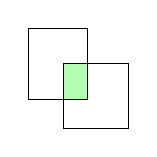
\begin{tikzpicture}[scale=0.75]
		\draw (0,0) rectangle (1,1.2);
		\draw (0.6,0.6) rectangle (1.7,-0.5);
		\draw[fill=green!30] (0.6,0.6) rectangle (1,0);
		\end{tikzpicture}
		\item \abs 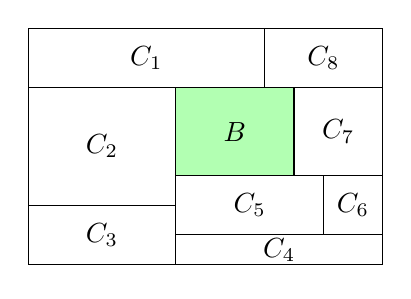
\begin{tikzpicture}[scale=0.75]
		\draw (0,0) rectangle (6,4);
		\draw[fill=green!30] (2.5,1.5) rectangle (4.5,3);		
		\draw (3.5, 2.25) node {$B$};
		\draw (0,4) rectangle (4,3);		
		\draw (2, 3.5) node {$C_1$};
		\draw (0,3) rectangle (2.5,1);
		\draw (1.25, 2) node {$C_2$};
		\draw (2.5,1.5) rectangle (5,0.5);
		\draw (3.75, 1) node {$C_5$};s
		\draw (4,4) rectangle (6,3);
		\draw (5, 3.5) node {$C_8$};
		\draw (4.5,3) rectangle (6,1.5);
		\draw (5.25, 2.25) node {$C_7$};
		\draw (0,1) rectangle (2.5,0);
		\draw (1.25, 0.5) node {$C_3$};
		\draw (2.5,0) rectangle (6,0.5);
		\draw (4.25, 0.25) node {$C_4$};
		\draw (5,1.5) rectangle (6,0.5);
		\draw (5.5, 1) node {$C_6$};
		\end{tikzpicture}
	\end{enumerate}
	Nat\"urlich kann man das formell sauber hinschreiben, das gibt uns aber keinen Verst\"andnis Mehrwehrt.
\end{beispiel1}
Aus der zweiten Eigenschaft eines Semirings kann man durch Induktion sofort Abgeschlossenheit bez\"uglich endlich vielen Schnitten zeigen. Probiert's einfach aus, ist zu einfach als \"Ubungsaufgabe. Auch die letzte Eigenschaft kann man verallgemeinern. Bei Quadern ist das anschaulich klar: Wenn man aus einem Quader endlich viele Quader entfernt, bleibt eine disjunkte Vereinigung von Quadern \"ubrig. Mit Induktion kriegen wir das auch f\"ur allgemeine Semiringe hin: 
\begin{lemma}\label{Skriptschreiberlemma} \link{https://www.youtube.com/watch?v=eLWjBR34aC0&list=PLy5qRKPWp6SBwfc1kn-b66cWc84cOgvqZ&index=4&t=4446s} \textbf{[Eine kleine Indexschlacht]}
	Es gilt in einem Semiring auch $\text{(iii)}'$: Sind $B_1,...,B_r,A\in \mathcal S$ mit  $B_1,B_2,...,B_r$ paarweise disjunkt, so existieren $C_1,...,C_n \in \cS$ paarweise disjunkt mit \[A \backslash (B_1 \cupdot ... \cupdot B_r) = \bigcupdot\limits_{k=1}^{n} C_k.\]
\end{lemma}

\begin{proof}
	Vollständige Induktion bezüglich $r$. \begin{itemize}
		\item [IA:] Für $A \backslash B_1$ folgt das direkt aus der Definition des Seminrings.
		\item [IV:] Die Behauptung gelte für ein beliebiges aber festes $r \in \N$.
		\item [IS:] Seien nun $B_1,B_2,...,B_{r+1} \in \mathcal S$ paarweise disjunkt. Nach Induktionsvoraussetzung und Rechenregeln mit Schnitten von Mengen gilt mit Umklammern von Schnitten und Vereinigungen
		\begin{align*}
		A \backslash \bigcupdot\limits_{i = 1}^{r+1} B_i &= A\cap  \bigcap_{i=1}^{r+1} B_i^C\\
		 &= \Big(A\backslash \bigcupdot_{i=1}^r B_i\Big) \cap B_{r+1}^C\\
		 & \overset{\text{IV}}{=} \Big(\bigcupdot\limits_{k = 1}^{m_r}  C_{r,k}\Big) \cap  B_{r + 1}^C
		 =\bigcupdot\limits_{k = 1}^{m_r} [C_{r,k} \backslash B_{r + 1}].
		\end{align*}
		Nun existieren für alle $1 \leq k \leq m_r$ jeweils endlich viele paarweise disjunkte Mengen $C_{r,k,1},...,C_{r,k,l_{r,k}} \in \cS$, mit 
		\[ C_{r,k} \backslash B_{r + 1} = \bigcupdot\limits_{m = 1}^{l_{r,k}} C_{r,k,m}. \]
		Also gilt \[
		A \backslash \bigcup\limits_{i = 1}^{r+1} B_i = \bigcupdot\limits_{k = 1}^{m_r} \bigcupdot\limits_{m = 1}^{l_{r,k}} C_{r,k,m}. \]
		Da die endlich vielen Mengen $C_{r,k,m}$ paarweise disjunkt sind, haben wir die gewünschte Darstellung f\"ur $A \backslash (B_1 \cupdot ... \cupdot B_{r+1})$ gefunden.
	\end{itemize}
\end{proof}
%Weiter geht es mit einer Versch\"arfung von Semiringen:
%\begin{deff}\label{Ring}
%	$\cR \in \cP(\Omega)$ heißt Ring, falls
%	\begin{enumerate}[label=(\roman*)]
%		\item $\emptyset \in \cR$
%		\item $A, B \in \cR \Rightarrow A \backslash B \in \cR$
%		\item $A,B \in \cR \Rightarrow A \cup B \in \cR$
%	\end{enumerate}
%\end{deff}

%\begin{bem1} \abs
%	\begin{enumerate}[label=(\roman*)]
%		\item $A^C$ ist nicht unbedingt in $\cR$, denn $\Omega \in \cR$ muss nicht gelten. Das sieht %harmlos aus, macht uns das Leben aber deutlich schwieriger.
%		\item Mit vollständiger Induktion sind auch endliche Vereinigungen wieder in $\cR$.
%	\end{enumerate}
%\end{bem1}



\marginpar{\textcolor{red}{Vorlesung 4}}


%\begin{bem}
%	$\cR$ Ring $\Rightarrow \cR$ Semiring. 
%\end{bem}

%\begin{proof}\abs
%	\begin{enumerate}[label=(\roman*)]
%		\item $\checkmark$
%		\item Folgt sofort aus der Beobachtung $A \cap B = A \backslash (A \backslash B)$.
%		\item Folgt sofort mit $n=1$, denn $A \backslash B \in \cR$.
%	\end{enumerate}
%\end{proof}

%Um ein besseres Gef\"uhl f\"ur die Definitionen zu bekommen, zeigen wir, dass die Menge der altbekannten disjunkten Vereinigungen von Quadern ein Ring bildet. Allgemeiner geht das f\"ur beliebige Semiringe:

%\begin{bem}
%	Ist $\cS$ ein Semiring, so ist die Menge aller endlicher disjunkter Vereinigungen
%	\[ \cR := \left\{ \bigcupdot\limits_{i = 1}^{n} A_i \! : n \in \N, \: A_1,...,A_n \in \cS \right\} \]
%	der kleinste Ring, der $\cS$ enth\"alt.
	% die Formulierung im Skript von Gärtner finde ich persönlich hübscher: "Man kann auf natürliche Weise aus jedem Semiring S einen Ring R konstruieren."
%\end{bem}

%\begin{proof}
%	Dass $\cR$ der \textit{kleinste} Ring ist, ist klar (es gilt $\cS \subseteq \cR$ mit $n=1$ und damit m\"ussen aufgrund der Eigenschaft eines Rings alle endlichen Vereinigungen wieder enthalten sein). Wir m\"ussen also noch zeigen, dass $\cR$ tats\"achlich ein Ring ist. Checken wir also die Eigenschaften:
%	\begin{enumerate}[label=(\roman*)]
%		\item $\checkmark$
%		\item \label{A,B} Seien dazu $A, B\in \cR$, also
%		\begin{gather*}
%			A = \bigcupdot\limits_{i=1}^{n} A_i\quad \text{ und }\quad  B = \bigcupdot\limits_{j=1}^{m} B_j.
%		\end{gather*}
%		Dann gilt
%			\begin{gather*}
%			A \backslash B = \bigcupdot\limits_{i=1}^{n} \underbrace{\Big( A_i \backslash \bigcupdot\limits_{j=1}^{m} \underbrace{(A_i \cap B_i)}_{\substack{\in \cS \text{, weil }\\ \cS \: \cap \text{-stabil}}}\Big)}_{\overset{\text{\ref{Skriptschreiberlemma}}}{=} \bigcupdot \limits_{k=1}^{r} C_{i,k}}\\
%			= \bigcupdot \limits_{i=1}^{n} \bigcupdot \limits_{k=1}^{r_i} C_{i,k}.
%		\end{gather*}
%		\item Seien $A,B$ wie in \ref{A,B}, so gilt $ A \cup B = \underbrace{(A\backslash B)}_{\in \cR} \cupdot \underbrace{B}_{\in \cR} \overset{\text{Def.}}{\in} \cR$ weil eine disjunkte Vereinigungen disjunkter Mengen in $\mathcal S$ wieder eine disjunkte Vereinigung von Mengen in $\mathcal S$ ist.
%	\end{enumerate}
%\end{proof}

%\begin{deff}
%	$\cA \subseteq \cP(\Omega)$ heißt Algebra, falls $\cA$ ein Ring ist und $\Omega \in \cA$.
%\end{deff}
%Die Definition einer Algebra ist \"aquivalent zur Forderung
%	\begin{enumerate}[label=(\roman*)]
%		\item $\emptyset \in \cA$,
%		\item $A \in \cA \Rightarrow A^C \in \cA$,
%		\item $A_1,...,A_n \in \cA \Rightarrow \bigcup\limits_{i = 1}^{n} A_i \in \cA$,
%	\end{enumerate}
%weil $\Omega\backslash A=A^C$.
%\begin{deff}
%	$\cR \subseteq \cP(\Omega)$ heißt $\sigma$-Ring, falls (iii) in der Definition des Rings durch 
%	\begin{align*}
%		A_1,A_2,... \in \cR \Rightarrow \bigcup\limits_{i = 1}^{\infty} A_i \in \cR 
%	\end{align*}
%	ersetzt wird. Das $\sigma$ steht also wieder für \enquote{abzählbar viele}.
	% Wir haben bei der ersten Definition des Maßes schon so nen ähnlichen Satz; ist nicht schlimm, aber könnte man evtl. auch in nur einen Satz zusammenführen.
%\end{deff}
%	Ein $\sigma$-Ring $\cR$ mit $\Omega \in \cR$ ist also nichts anderes als eine $\sigma$-Algebra.

Es kommen jetzt ein paar schmerzhafte Vorbereitungen f\"ur den wichtigsten Satz dieses Abschnitts, den Fortsetztungssatz von Carath\'eodory. Wir werden zun\"achst zeigen, dass die Monotonie und Subadditivit\"at (siehe Lemma \ref{monsub}) auch f\"ur \glqq Ma\ss e\grqq{} auf Semiringen gilt. Warum steht hier Ma\ss{} in Anf\"uhrungsstrichen? Per Definition ist ein Ma\ss{} immer auf einer $\sigma$-Algebra definiert, der Begriff macht also auf Semiringen gar keinen Sinn. Die genaue Aussage ist also, dass eine Mengenfunktion auf Semiringen mit Eigenschaften die einem Ma\ss{} \"ahneln, ebenfalls Monotonie und Subadditivit\"at erf\"ullen. 
\begin{lemma}\label{Rechenregeln} \link{https://www.youtube.com/watch?v=P2eNjbbLRa8&list=PLy5qRKPWp6SBwfc1kn-b66cWc84cOgvqZ&index=5&t=275s}\textbf{[Eine ziemlich gro\ss e Indexschlacht]}
	Sei $\cS$ ein Semiring und $\mu \! : \mathcal S \rightarrow [0, \infty] $ eine Mengenfunktion mit
	\begin{itemize}
		\item $\mu(\emptyset) = 0$
		\item $\mu$ ist \textbf{$\sigma$-additiv} (d.h. sind $A_1, A_2, ... \in S$ paarweise disjunkt mit $A:=\bigcupdot_{k=1}^\infty A_k\in \mathcal S$, so gilt $\mu(A)=\sum_{k=1}^\infty \mu(A_k)$).
	\end{itemize}
	Dann gilt
	\begin{enumerate}[label=(\roman*)]
		\item \label{MonotQuasiMass} Monotonie: $\mu(A) \leq \mu(B)$ für alle $A,B \in \cS$ mit $ A \subseteq B$.
		\item  \glqq \textbf{Subadditivit\"at}\grqq: Sind $A,A_1,A_2,... \in \cS $ und $A\subseteq \bigcup\limits_{k=1}^{\infty} A_k$, so gilt $ \mu(A) \leq \sum\limits_{k = 1}^{\infty} \mu(A_k).$
	\end{enumerate}
\end{lemma}
Man beachte, dass die Eigenschaften der $\sigma$-Additivit\"at etwas komisch sind. Da wir nicht fordern, dass Semiringe abgeschlossen bez\"uglich Vereinigungen sind (sie sind es auch meistens nicht, man denke nur an den Semiring der Quader), muss immer gefordert werden, dass die Vereinigungen wieder in $\cS$ liegen. Sonst w\"are $\mu(A)$ schlie\ss lich gar nicht definiert! Auch zu beachten ist, dass Vereinigungen und Komplemente nicht automatisch in $\mathcal S$ liegen. Daher sind einfache Eigenschaften f\"ur Ma\ss e auf $\sigma$-Algebren, nicht so einfach f\"ur Mengenfunktionen auf Semiringen.

\begin{proof}\abs
	\begin{enumerate}[label=(\roman*)]
		\item Es gibt wegen der Eigenschaften eines Semirings Mengen $C_1,...,C_m \in \cS$ mit \[B \backslash A = \bigcupdot\limits_{k=1}^m C_k.\] Damit gilt wegen der geforderten Additivit\"at von $\mu$
		\begin{align*}
		\mu(B) &= \mu(A \cupdot (B \backslash A)) = \mu(A \cupdot C_1 \cupdot ... \cupdot C_m) = \mu(A) + \mu(C_1) + ... + \mu(C_m)
		\geq \mu(A).
		\end{align*} 
		\item Erst machen wir (wie immer wieder!) die $A_n$ disjunkt:
		\begin{align*}
			A'_1 &:= A_1,\\
			A_2' &:= A_2 \backslash A_1',\\
			A_n' &:= A_n \backslash (A_1' \cupdot ... \cupdot A_{n-1}' ), \quad n \geq 3.
		\end{align*}
		\textit{Beachte:} Die $A'_{n}$ müssen nicht in in $\cS$ sein. Weil die $A'_{n}$ die Form $A_n \backslash ...$ haben, gibt es wegen Lemma \ref{Skriptschreiberlemma} allerdings paarweise disjunkte $C_{n,j} \in \cS$ mit 
		\begin{equation}\label{C_ns}
			A_{n}' = \bigcupdot\limits_{j=1}^{l_n} C_{n,j}
		\end{equation}
		für alle $n \in \N$. Darum gibt es wegen Lemma \ref{Skriptschreiberlemma} Mengen $D_{n,k} \in \cS$ mit
		\begin{equation}\label{D_nks}
			A_n \backslash A_{n}' = \bigcupdot\limits_{k = 1}^{m_n} D_{n,k}.
		\end{equation}
		Damit gelten
		\begin{itemize}
			\item 
			\begin{equation*}
				A = \bigcupdot\limits_{n=1}^{\infty} A'_{n} \cap A = \bigcupdot\limits_{n=1}^{\infty} \bigcupdot\limits_{j=1}^{l_n} A \cap C_{n,j}
			\end{equation*}
			weil $A\subseteq \bigcup\limits_{n=1}^{\infty} A_{n}= \bigcupdot\limits_{n=1}^{\infty} A_{n}'$ angenommen wurde,
			\item 
			\begin{gather*}
				A_n = A'_{n} \cupdot (A_n \backslash A'_{n}) \underset{\eqref{D_nks}}{\overset{\eqref{C_ns}}{=}} \bigcupdot\limits_{j=1}^{l_n} C_{n,j} \cupdot \bigcupdot\limits_{n = 1}^{m_n} D_{n,k}.
			\end{gather*}
		\end{itemize}
	Alles zusammen ergibt die Subadditivit\"at:
	\begin{align*}
		\mu(A) &= \mu\Big(\bigcupdot\limits_{n=1}^{\infty} \bigcupdot\limits_{j=1}^{l_n} \underbrace{A \cap C_{n,j}}_{\substack{\in \cS \text{, weil }\mathcal S\\ \cap \text{-stabil}}}\Big) \\
		\overset{\sigma \text{-add.}}&{=} \sum\limits_{n=1}^{\infty} \sum\limits_{j=1}^{l_n} \mu(A \cap C_{n,j}) \\ 
		\overset{\text{Monotonie}}&{\leq} \sum\limits_{n=1}^{\infty} \sum\limits_{j=1}^{l_n} \mu(C_{n,j}) \\
		\overset{\mu \geq 0}&{\leq} \sum\limits_{n=1}^{\infty} \Big( \sum\limits_{j=1}^{l_n} \mu(C_{n,j}) + \sum\limits_{k=1}^{m_n} \mu(D_{n,k})\Big) \\ 
		\overset{\sigma \text{-add.}}&{=} \sum\limits_{n=1}^{\infty} \mu\Big(\bigcupdot\limits_{n=1}^{l_n} C_{n,j} \cupdot \bigcupdot\limits_{j=1}^{m_n} D_{n,k}\Big)\\
		& = \sum\limits_{n=1}^{\infty} \mu(A_n).
	\end{align*}
	\end{enumerate}
\end{proof}
\begin{deff} \link{https://www.youtube.com/watch?v=P2eNjbbLRa8&list=PLy5qRKPWp6SBwfc1kn-b66cWc84cOgvqZ&index=5&t=2204s}
	$\mu^{*} \! : \cP (\Omega) \rightarrow [0,\infty]$ heißt \textbf{äußeres Maß}, falls
	\begin{enumerate}[label=(\roman*)]
		\item $\mu^{*}(\emptyset) = 0$
		\item $A \subseteq B \subseteq \Omega\, \Rightarrow \, \mu^{*}(A) \leq \mu^{*}(B)$
		\item $A_1,A_2,... \subseteq \Omega \, \Rightarrow \, \mu^{*} \Big(\bigcup\limits_{k=1}^{\infty} A_k \Big) \leq \sum\limits_{k=1}^{\infty} \mu^{*}(A_k)$
	\end{enumerate}
\end{deff}
F\"ur den Moment bleibt es unklar, weshalb wir dieser abstrakten Definition den Namen \glqq \"au\ss eres Ma\ss\grqq{} geben. Das wird aber in dem Beweis des Carath\'eodory Fortsetzungssatzes klar werden. Das dort definierte \"au\ss ere Ma\ss{} hat eine klare Interterpretation.
\begin{deff}\link{https://www.youtube.com/watch?v=P2eNjbbLRa8&list=PLy5qRKPWp6SBwfc1kn-b66cWc84cOgvqZ&index=5&t=2376s}
	Sei $\mu^{*}$ ein äußeres Maß auf $\Omega$. Dann heißt $A \subseteq \Omega$ \textbf{$\mu^{*}$-messbare Menge}, falls für alle $Z \subseteq \Omega$ \[ \mu^{*}(Z) = \mu^{*}(Z\cap A) + \mu^{*}(Z \cap A^C) \] gilt. Die Menge der $\mu^{*}$-messbaren Mengen heißt $\cA_{\mu^{*}}$.
\end{deff}

\begin{prop}
\link{https://www.youtube.com/watch?v=P2eNjbbLRa8&list=PLy5qRKPWp6SBwfc1kn-b66cWc84cOgvqZ&index=5&t=2556s} \abs 
	\begin{enumerate}[label=(\roman*)]		
		\item $\cA_{\mu^{*}}$ ist eine $\sigma$-Algebra.
		\item $\mu^{*}$ eingeschränkt auf $\cA_{\mu^{*}}$ ist ein Maß.
	\end{enumerate}
\end{prop}

\begin{proof}
	Wir zeigen nacheinander (a) $\cA_{\mu^{*}}$ ist eine $\sigma$-Algebra und (b) $\mu^{*}$ ist ein Maß auf $\cA_{\mu^{*}}$.\smallskip
	
	(a) Zu zeigen sind die definierenden Eigenschaften einer $\sigma$-Algebra:
		\begin{enumerate}[label=(\roman*)]
			\item F\"ur $Z \subseteq \Omega$ gilt 
			\begin{gather*}
			\mu^{*}(Z) = \mu^{*}(Z) + 0 = \mu^{*}(Z \cap \Omega) + \mu^{*}(Z \cap \underbrace{\Omega^C}_{= \emptyset}).
			\end{gather*}
			Damit ist $\Omega \in \cA_{\mu^{*}}$ gezeigt.
			\item Sei $A \in \cA_{\mu^{*}}$, dann erf\"ullt ($+$ kommutieren und $(A^C)^C=A$ nutzen) auch $A^C$ die definierende Eigenschaft von $\cA_{\mu^{*}}$. Also ist $\cA_{\mu^{*}}$ abgeschlossen unter Komplementbildung.
			\item Wir zeigen zun\"achst die Abgeschlossenheit bez\"uglich Vereinigungen von zwei Mengen. Seien also $A_1, A_2 \in \cA_{\mu^{*}}$. Sei $Z \subseteq \Omega$ beliebig, dann folgt mit $Z':= Z\cap (A_1\cup A_2)$
			\begin{align*}
			\mu^{*}(Z \cap (A_1 \cup A_2))
			\overset{A_1 \in \cA_{\mu^{*}}}&{=} \mu^*(Z\cap(A_1\cup A_2)\cap A_1)+\mu^*(Z\cap(A_1\cup A_2)\cap A_1^C)\\
			&= \mu^{*}(Z \cap A_1) + \mu^{*}(Z \cap A_2 \cap A_1^C).
			\end{align*}
			Folglich gilt auch
			\begin{align*}
			&\quad \mu^{*}(Z \cap (A_1 \cup A_2)) + \mu^{*}(Z \cap (A_1 \cup A_2)^C)\\
			&= \mu^{*}(Z \cap A_1) + \mu^{*}(Z \cap A_2 \cap A_1^C) + \mu^{*}(Z \cap (A_1 \cup A_2)^C)&\\
			&= \mu^{*}(Z \cap A_1) + \mu^{*}(\underbrace{Z \cap A_1^C}_{=: Z''} \cap A_2) + \mu^{*}(\underbrace{Z \cap A_1^C}_{=: Z''} \cap A_2^C)&\\
			\overset{A_2 \in \cA_{\mu^{*}}}&{=} \mu^{*}(Z \cap A_1) + \mu^{*}(Z \cap A_1^C)\\\overset{A_1 \in \cA_{\mu^{*}}}&{=} \mu^{*}(Z)
			\end{align*}
			und damit ist $A_1\cup A_2 \in \cA_{\mu^{*}}$.
		\item Per Induktion folgt aus (iii) die Abgeschlossenheit bez\"uglich Vereinigungen endlich vieler Mengen.
		\item Es fehlt jetzt noch die Abgeschlossenheit bez\"uglich abz\"ahlbar unendlicher Vereinigungen.
 Seien also $A_1,A_2,...\in \cA_{\mu^{*}}$, zu zeigen ist $\bigcup\limits_{n=1}^{\infty} A_n \in \cA_{\mu^{*}}.$ Zuerst nutzen wir den schon bekannten Trick, der uns erlaubt, ohne Einschr\"ankung der Allgemeinheit anzunehmen, dass die Mengen diskjunkt sind. Dazu definieren wir die paarweise disjunkten Mengen
	\begin{align*}
		A_1'=A_1, \quad A_2'=A_2\backslash A_1',\quad \text{ und }\quad A_n'= A_n \backslash (A_1' \cupdot ...\cupdot A_{n-1}'), \quad n \geq 3,
	\end{align*}
	und beachten, dass damit $\bigcup\limits_{n=1}^{\infty} A_n = \bigcupdot\limits_{n=1}^{\infty} A_n'$ gilt. Wenn also die Vereinigung der disjunkten $A_n'$ wieder in $\mathcal A_{\mu^*}$ ist, ist auch die Vereinigung \"uber die $A_n$ in $\mathcal A_{\mu^*}$. Es reicht also die Aussage f\"ur disjunkte Mengen zu beweisen. Damit die Rechnungen lesbarer bleiben, nehmen wir also ohne Beschr\"ankung der Allgemeinheit an, dass die Mengen $A_1, A_2, ...$ paarweise disjunkt sind, so sparen wir uns die $'$ in den Gleichungen. Aufgrund der Definition von $\mathcal A_{\mu^*}$ w\"ahlen wir ein $Z\subseteq \Omega$ beliebig. Wir zeigen erstmal induktiv 
	\begin{equation}\label{IndVor}
		\mu^{*}(Z)= \sum\limits_{k=1}^{n} \mu^{*}(Z \cap A_k) + \mu^{*}\Big(Z \cap \bigcap\limits_{k=1}^{n} A_k^C \Big),\quad \forall n \in \N.
	\end{equation}
	\begin{itemize}
		\item [IA:] Für $n=1$ gilt die Behauptung, weil $A_1 \in \cA_{\mu^{*}}$.
		\item [IV:] Es gelte \eqref{IndVor} für ein \underline{beliebiges, aber festes} $n \in \N$.
		\item [IS:] Eine kleine Runde Kampfrechnen mit Mengen. Weil nach Annahme $A_{n+1} \in \cA_{\mu^{*}}$ und die $A_n$ paarweise disjunkt sind, gilt
		\begin{align*}
			\mu^{*}\Big(Z \cap \bigcap\limits_{k=1}^{n} A_k^C \Big)
			&= \mu^{*}\Big(Z \cap \bigcap\limits_{k=1}^{n} A_k^C \cap A_{n+1} \Big) + \mu^{*}\Big(Z \cap \bigcap\limits_{k=1}^{n} A_k^C \cap A_{n+1}^C \Big)\\
			 &= \mu^{*}(Z \cap A_{n+1})+ \mu^{*}\Big(Z \cap \bigcap\limits_{k=1}^{n + 1} A_k^C \Big).
		\end{align*}
		Einsetzen in die Induktionsvoraussetzung gibt
		\begin{align*}
			\mu^{*}(Z) & = \sum\limits_{k = 1}^{n + 1} \mu^{*}(Z \cap A_k) + \mu^{*}\Big(Z \cap \bigcap\limits_{k=1}^{n + 1} A_k^C \Big).
		\end{align*}
		Damit ist der Induktionsschritt gezeigt.
	\end{itemize}
	Zur\"uck zur Vereinigung: Wegen der angenommenen Monotonie von $\mu^*$ folgt aus \eqref{IndVor}  \[ \mu^{*}(Z) \geq \sum\limits_{k=1}^{n} \mu^{*}(Z \cap A_k) + \mu^{*}\Big(Z \cap \bigcap\limits_{k = 1}^{\infty} A_k^C\Big), \quad \forall n \in \N. \]
		Mit $n \to \infty$ folgt (Monotonie von Grenzwertbildung aus Analysis 1)
		\begin{align}\label{ab}
		\begin{split}
			\mu^{*}(Z) &\geq \sum\limits_{k=1}^{\infty} \mu^{*}(Z \cap A_k) + \mu^{*}\Big(Z \cap \bigcap\limits_{k = 1}^{\infty} A_k^C\Big)\\ 
			&\geq \mu^{*} \Big(\bigcup\limits_{k = 1}^{\infty} A_k \cap Z \Big) + \mu^{*}\Big(Z \cap \Big(\bigcup\limits_{k = 1}^{\infty} A_k\Big)^C\Big)\\
			&\geq  \mu^{*}\Big(\Big(Z \cap \bigcup\limits_{k = 1}^{\infty} A_k\Big) \cup \Big(Z\cap \Big(\bigcup\limits_{k = 1}^{\infty} A_k\Big)^C\Big)\Big)\\
			& = \mu^{*}\Big(Z \cap \underbrace{\Big(\bigcup\limits_{k= 1}^{\infty} A_k\cup \Big(\bigcup\limits_{k= 1}^{\infty} A_k\Big)^C\Big)}_{\Omega}\Big) = \mu^{*}(Z).
		\end{split}
		\end{align}
		F\"ur die letzten beiden Ungleichungen haben wir die angenommene Subadditivit\"at (Ungleichung andersrum als \"ublich) genutzt. 
	Weil die linke und rechte Seite der Kette von Ungleichungen identisch sind, sind die Ungleichungen alles Gleichungen, also gilt \[ \mu^{*}(Z) = \mu^{*}\Big(Z \cap \bigcup\limits_{k=1}^{\infty} A_k\Big) + \mu^{*}\Big(Z \cap \Big(\bigcup\limits_{k=1}^{\infty} A_k\Big)^C\Big).  \] Weil $Z$ beliebig war, ist damit \[ \bigcup\limits_{k=1}^{\infty} A_k \in \cA_{\mu^{*}} \] aufgrund der Definition von $\mathcal A_{\mu^*}$.	Damit ist die Abgeschlossenheit bez\"uglich abz\"ahlbarer Vereinigungen gezeigt und folglich ist $\cA_{\mu^{*}}$ eine $\sigma$-Algebra. 
		\end{enumerate}

	
	(b) Aufgrund der Gleichheiten in \eqref{ab} gilt auch
	 \[ \mu^{*}(Z) = \sum\limits_{k = 1}^{\infty} \mu^{*}(Z \cap A_k) + \mu^{*}\Big(Z \cap \bigcap\limits_{k = 1}^{\infty} A_k^C\Big). \] 
	Wählen wir  $	Z = \bigcup\limits_{k = 1}^{\infty} A_k$, so gilt wegen $\mu(\emptyset)=0$
	\begin{align*}
		 \mu^{*}\Big(\bigcup\limits_{k = 1}^{\infty} A_k\Big)=\sum\limits_{k = 1}^{\infty} \mu^{*}(A_k) + 0
	\end{align*}
	und das ist gerade die $\sigma$-Additivit\"at von $\mu^*$. Also ist $\mu^*$ auch ein Ma\ss{} auf der $\sigma$-Algebra $\mathcal A_{\mu^*}$.
\end{proof}
\marginpar{\textcolor{red}{Vorlesung 5}}
Kommen wir endlich zum H\"ohepunkt der ersten Wochen. Nach dem Beweis sind wir auch endlich mitten in der Stochastik angelangt! Der Beweis enth\"alt tats\"achlich viele Informationen. Insbesondere wird klar, wo der Begriff \"au\ss eres Ma\ss{} herkommt.
\begin{satz} \label{KarlTheodor} \link{https://www.youtube.com/watch?v=nlUyBvwBkhE&list=PLy5qRKPWp6SBwfc1kn-b66cWc84cOgvqZ&index=6&t=164s} \textbf{[Fortsetzungssatz von Carathéodory]}
	Sei $\cS$ ein Semiring und $\mu \! : \mathcal S \rightarrow [0, \infty] $ eine Mengenfunktion mit
	\begin{itemize}
		\item $\mu(\emptyset) = 0$,
		\item $\mu$ ist \textbf{$\sigma$-additiv} (d.h. sind $A_1, A_2, ... \in S$ paarweise disjunkt mit $A:=\bigcupdot_{k=1}^\infty A_k\in \mathcal S$, so gilt $\mu(A)=\sum_{k=1}^\infty \mu(A_k)$).
	\end{itemize}
	Dann existiert ein Maß $\bar{\mu}$ auf $\sigma(\mathcal S)$ mit $\mu(A) = \bar{\mu}(A)$ für alle $A \in \cS$.
\end{satz}
Man sagt, dass die Mengenfunktion $\mu$ von $\cS$ nach $\sigma(\cS)$ \glqq fortgesetzt\grqq{} wird.

\begin{proof}
	Für $A \in \cP(\Omega)$ definieren wir \[ \mu^{*}(A) = \inf\Big\{ \sum\limits_{k=1}^{\infty} \mu(A_k) \! : A_1,A_2,... \in \cS \text{ mit } A \subseteq \bigcup\limits_{k = 1}^{\infty} A_k \Big\}. \]
	Beachte: Weil per Definition (Analysis 1) $\inf \emptyset=+\infty$ gilt, ist $\mu*(A)$ auch definiert, wenn man $A$ nicht durch Mengen aus $\mathcal S$ \"uberdecken kann. \smallskip
	
	Wir zeigen nun nacheinander (a) $\mu^*$ ist ein \"au\ss eres Ma\ss{}, (b) $\cS \subseteq \mathcal A_{\mu^*}$ und (c) $\mu^*(A)=\mu(A)$ f\"ur alle $A\in \cS$. Der Beweis ist dann vollendet, weil nach dem vorherigen Satz $\mathcal A_{\mu^*}$ eine $\sigma$-Algebra ist und $\mu^*$ ein Ma\ss{} auf $\mathcal A_{\mu^*}$ ist. Wegen (b) gilt $\sigma(S)\subseteq \mathcal A_{\mu^*}$, weil die kleinste $\sigma$-Algebra die $\cS$ enth\"alt, auch Teilmenge von allen $\sigma$-Algebras ist, die $\cS$ enthalten. Damit ist auch die Einschr\"ankung von $\mu^*$ auf $\sigma(S)$ ein Ma\ss{} (wir setzen dann $\bar{\mu} := \mu^{*}_{|{\sigma(\cS)}}$) und wegen (c) ist $\bar\mu$ eine Fortsetzung von $\mu$.
\begin{enumerate}[label=(\alph*)]
\item	Wir checken die definierenden Eigenschaften eines \"au\ss eren Ma\ss es:
	\begin{itemize}
		\item[(i)] $\mu^{*}(\emptyset) = 0$ ist klar, weil $\emptyset \in \mathcal S$ und $\mu(\emptyset)=0$.
		\item[(ii)] Monotonie folgt direkt aus der Definition.
		\item[(iii)] Nun zur Subadditivität. Seien dazu $A_1,A_2,... \in \mathcal P(\Omega)$ und $A = \bigcup\limits_{k = 1}^{\infty} A_k.$ Wir k\"onnen annehmen, dass $ \: \mu^{*}(A_k) < \infty$ f\"ur alle $k\in\N$ gilt (sonst gilt die Ungleichung sowieso). Sei nun $\varepsilon > 0$ beliebig. Für jedes $k \in \N$ existiert qua Definition (Infimum ist die gr\"o\ss te untere Schranke) eine Folge von Mengen $A_{k,1},A_{k,2},... \in \cS$ mit
		\begin{align*}
			A_k \subseteq \bigcup\limits_{j=1}^{\infty} A_{k,j} \quad \text{ und }\quad \sum\limits_{j=1}^{\infty} \mu(A_{k,j}) \leq \mu^{*}(A_k) + \frac{\varepsilon}{2^k}.			\end{align*}
		Wem das nicht klar ist, der schaue bitte in den Analysis 1 Mitschrieb! Weil \[A \overset{\text{Def.}}{=} \bigcup\limits_{k = 1}^{\infty} A_k \subseteq \bigcup\limits_{k = 1}^{\infty} \bigcup\limits_{j=1}^{\infty} A_{k,j} \] gilt, folgt (das Infimum einer Menge ist kleiner gleich jedem Element der Menge) 
		\begin{gather*}
			\mu^{*}(A) \underset{\text{als } \inf}{\overset{\text{Def. } \mu^{*}}{\leq}} \sum\limits_{k= 1}^{\infty} \sum\limits_{j= 1}^{\infty} \mu(A_{k,j}) \leq \sum\limits_{k = 1}^{\infty} \Big( \mu^{*}(A_k) + \frac{\varepsilon}{2^k} \Big) = \sum\limits_{k = 1}^{\infty} \mu^{*}(A_k) + \underbrace{\sum_{k=1}^\infty \frac{\varepsilon}{2^k}}_{\varepsilon}.
		\end{gather*}
		Weil $\varepsilon$ beliebig gew\"ahlt wurde, gilt damit die Subadditivit\"at von $\mu^*$. An dieser Stelle eine kleine Anmerkung: Eine \"Uberdeckung durch eine abz\"ahlbare Vereinigung von abz\"ahlbaren Vereinigungen ist gleichbedeutend zu nur einer abz\"ahlbaren Vereinigung. Das Stichwort ist Cantors Diagonalverfahren, siehe Analysis 1 (oder irgendeine andere Quelle). Wir k\"onnen Paare von nat\"urlichen Zahlen auf verschiedenen Weisen z\"ahlen: Zeilenweise, Spaltenweise, oder wie eine Schlange im Diagonalverfahren.
	\end{itemize}
	\item 	
		Wir zeigen $\cS \subseteq \cA_{\mu^{*}}$. Dazu m\"ussen wir $$\mu^{*}(Z) = \mu^{*}(Z \cap S) + \mu^{*}(Z \cap S^C),\quad \text{für alle }Z \subseteq \Omega, S \in \cS,$$ nachrechnen.
		
		\enquote{$\leq$}: $\mu^{*}(Z) = \mu^{*}((Z \cap S )\cupdot (Z \cap S^C)) \leq \mu^{*}(Z \cap S) + \mu^{*}(Z \cap S^C)$ gilt aufgrund der gezeigten Subadditivit\"at von $\mu^*$.
		
		\enquote{$\geq$}: Seien $A_1,A_2,... \subseteq \cS$ mit $Z \subseteq \bigcup\limits_{k= 1}^{\infty} A_k.$ Weil $\cS$ ein Semiring ist, existieren $C_{k,1},..., C_{k,m_k} \in \cS$ mit \[ A_k \cap S^C = A_k \backslash S = \bigcupdot\limits_{j= 1}^{m_k} C_{k,j}. \]
		Es gelten 
			 \[ Z \cap S \subseteq \Big(\bigcup\limits_{k = 1}^{\infty} A_k\Big) \cap S = \bigcup\limits_{k = 1}^{\infty} \big( A_k \cap S \big) \]
			 sowie analog
			 \[ Z \cap S^C \subseteq  \Big(\bigcup\limits_{k = 1}^{\infty} A_k\Big) \cap S^C= \bigcup\limits_{k = 1}^{\infty} \big( A_k \cap S^C \big)=\bigcup\limits_{k = 1}^{\infty}\bigcupdot\limits_{j= 1}^{m_k} C_{k,j}. \]
		Mit den Definitionen folgt
		\begin{align*}
			\mu^{*} (Z \cap S) + \mu^{*} (Z \cap S^C) 
			&\leq \sum\limits_{k=1}^{\infty} \Big(\mu( A_k\cap S) +\sum\limits_{j=1}^{m_k} \mu(C_{k,j})\Big )\\
			\overset{\mu\,\sigma\text{-add.}}&{=} \sum\limits_{k=1}^{\infty} \mu \Big((A_k \cap S) \cupdot \bigcupdot\limits_{j=1}^{m_k} C_{k,j} \Big)\\
			& = \sum\limits_{k=1}^{\infty} \mu \big((A_k \cap S )\cupdot( A_k \cap S^C)\big)\\
			&=\sum_{k=1}^\infty \mu(A_k).
		\end{align*}
		Daraus folgt $\mu^{*}(Z \cap S) + \mu^{*}(Z \cap S^C) \leq \mu^{*}(Z)$, weil \[\mu^{*}(Z) = \inf\left\{ \sum\limits_{k=1}^{\infty} \mu(A_k) \! : A_1,A_2,... \in \cS \text{ mit } Z \subseteq \bigcup\limits_{k = 1}^{\infty} A_k \right\}.\] Somit ist \enquote{$\geq$} gezeigt.		
		Also ist jedes $S \in A_{\mu^{*}}$ und damit gilt $\cS \subseteq A_{\mu^{*}}$.
		
		\item Fehlt noch $\mu^{*}(A) = \mu(A)$ für alle $A \in \cS$. Im Prinzip ist das Lemma \ref{Rechenregeln}.\smallskip
		
		\enquote{$\leq$}: \[ \mu^{*}(A) = \inf\left\{ \sum\limits_{k=1}^{\infty} \mu(A_k) \! : A_1,A_2,... \in \cS \text{ mit } A \subseteq \bigcup\limits_{k = 1}^{\infty} A_k \right\} \leq \mu(A) \:  \]f\"ur alle $A\in \mathcal S$.
		
		\enquote{$\geq$}:  Ist $A \subseteq \bigcup\limits_{k=1}^{\infty} A_k$ f\"ur $A_1,A_2,... \in \cS$, 
		so gilt \[ \mu(A) \overset{\ref{Rechenregeln}}{\leq} \sum\limits_{k=1}^{\infty} \mu(A_k). \] Folglich gilt \[ \mu(A) \leq \inf\left\{ \sum\limits_{k=1}^{\infty} \mu(A_k) \! : A_1,A_2,... \in \cS \text{ mit } A \subseteq \bigcup\limits_{k = 1}^{\infty} A_k \right\} = \mu^{*}(A). \]		
		
	\end{enumerate}
\end{proof}
Wir fassen nun den Existenz- und den Eindeutigkeitssatz zusammen, das gibt folgendes zentrale Theorem:
\begin{satz}\label{ExistMasse} \link{https://www.youtube.com/watch?v=nlUyBvwBkhE&list=PLy5qRKPWp6SBwfc1kn-b66cWc84cOgvqZ&index=6&t=3820s} \textbf{[Existenz und Eindeutigkeit von Maßen] }
	Es sei $(\Omega, \cA)$ ein messbarer Raum, $\cE$ ein Semiring mit $\sigma(\cE) = \cA$ und $\mu \! : \cE \rightarrow [0,\infty]$ eine Mengenfunktion mit
	\begin{itemize}
		\item $\mu(\emptyset) = 0$
		\item $\mu$ ist $\sigma$-additiv
		\item es gibt eine Folge $E_1,E_2,... \in \cE$ mit $E_n \uparrow \Omega$ und $\mu(E_n) < \infty$ f\"ur alle $n\in\N$.
	\end{itemize}
	Dann existiert genau ein Maß $\bar{\mu}$ auf $\cA = \sigma(\cE)$, so dass $\bar{\mu}(A) = \mu(A)$ f\"ur alle $A\in \cE$.
\end{satz}

\begin{proof}
	Existenz folgt direkt aus \ref{KarlTheodor}, Eindeutigkeit folgt direkt aus Satz \ref{folg}.
\end{proof}
Merkt euch f\"ur immer folgendes, das hilft euch, die verschiedenen Konzepte einzuordnen:
\begin{center}
	\textbf{Existenz ist Carath\'eodory mit \"au\ss eren Ma\ss en, Eindeutigkeit folgt aus Dynkin-Systemen!}
\end{center}
Anschlie\ss end an die abstrakte Theorie wollen wir nun als Beispiel die Borel-$\sigma$-Algebra auf $\R$ diskutieren. Hier wird alles viel klarer werden und das ist gerade die Anwendung, die wir f\"ur die Stochastik brauchen.



\section[Das Beispiel f\"ur Wahrscheinlichkeitsma\ss e]{Das Beispiel - Wahrscheinlichkeitsmaße auf $\mathcal B(\R)$ aus Verteilungsfunktionen}\label{sec:VF}
Das Konzept von Verteilungsfunktionen von Wahrscheinlichkeitsma\ss en auf $\mathcal B(\R)$ ist euch bereits bei Dynkin-Systemen und in den \"Ubungen \"uber den Weg gelaufen. Definieren wir nun abstrakt, welche reellen Funktionen wir Verteilungsfunktionen nennen wollen:
\begin{deff}
\link{https://www.youtube.com/watch?v=nlUyBvwBkhE&list=PLy5qRKPWp6SBwfc1kn-b66cWc84cOgvqZ&index=6&t=4310s}
	$F \! : \mathbb{R} \rightarrow \mathbb{R}$ heißt \textbf{Verteilungsfunktion}, falls 
	\begin{enumerate}[label=(\roman*)]
		\item $0 \leq F(t) \leq 1$ f\"ur alle $t\in\R$,
		\item $F$ ist nicht fallend,
		\item $F$ ist rechtsstetig, \mbox{d. h.} $\lim\limits_{s \downarrow t} F(s) = F(t)$,
		\item $\lim\limits_{t \to \infty} F(t) = 1$ und $\lim\limits_{t \to - \infty} F(t) = 0$.
	\end{enumerate}
\end{deff}
Der Hauptsatz \"uber Wahrscheinlichkeitsma\ss e auf $\mathcal B(\R)$ ist nun folgender bijektiver Zusammenhang zu Verteilungsfunktionen:
\begin{satz}\label{EindVert}
\link{https://www.youtube.com/watch?v=nlUyBvwBkhE&list=PLy5qRKPWp6SBwfc1kn-b66cWc84cOgvqZ&index=6&t=4500s} \textbf{[Wahrscheinlichkeitsma\ss e aus Verteilungsfunktionen]}
	Für jede Vertei-lungsfunktion F gibt es \textbf{genau ein} Wahrscheinlichkeitsmaß $\mathbb{P}_F$ und $\cB(\mathbb{R})$ mit $$\mathbb{P}_F((-\infty,t]) = F(t), \quad t \in \mathbb R.$$ Man sagt dann, \enquote{$\mathbb{P}_F$ ist gemäß $F$ verteilt} oder \enquote{$\mathbb{P}_F$ hat Verteilung $F$} und schreibt $\mathbb{P}_F\sim F$.
\end{satz}

\begin{proof}
\textbf{Eindeutigkeit}: Das haben wir uns schon in Beispiel \ref{eindm} \"uberlegt.\smallskip

\textbf{Existenz}: Um den Fortsetzungssatz von Carath\'eodory zu nutzen, m\"ussen wir zun\"achst einen Semiring w\"ahlen, der die Borel-$\sigma$-Algebra erzeugt. Wir wissen bereits, dass alle m\"oglichen Arten von Intervallen $\mathcal B(\R)$ erzeugt, die meisten sind aber keine Semiringe. Wir nehmen $$\cS = \{ (a,b]: a\leq b \},$$ und stellen sofort fest (Eigenschaften checken), dass $\cS$ ein Semiring mit $\sigma(\cS) = \cB(\mathbb{R})$ ist. Als Mengenfunktion auf $\cS$ definieren wir $$\mu((a,b]): = F(b) - F(a),\quad a\leq b.$$ Weil $F$ nicht-fallend ist und $0\leq F\leq 1$ gilt, bildet $\mu$ nach $[0,1]$ ab. Checken wir als n\"achstes die Voraussetzungen vom Fortsetzungssatz:
	\begin{enumerate}[label=(\roman*)]
		\item $\mu(\emptyset) = \mu((a,a]) = F(a) -F(a) = 0$
		\item F\"ur die $\sigma$-Additivität von $\mu$ auf $\mathcal S$ seien $(a_n,b_n] \in \cS$ paarweise disjunkt mit \[
		\bigcupdot\limits_{k= 1}^{\infty} (a_k,b_k] \in \cS, \quad \text{ also } \bigcupdot \limits_{k = 1}^{\infty} (a_k,b_k] =: (a,b], \]
		f\"ur geeignete $a,b\in\R$. Als Anschauungsbeispiel haltet ihr am besten das konkrete Beispiel $(0,1] = \bigcupdot \limits_{k=1}^{\infty} (\frac{1}{k+1}, \frac{1}{k}]$ im Kopf. Um den Beweis besser zu verstehen, schauen wir uns erstmal den endlichen Fall an, d. h. \[ (a,b] = \bigcupdot\limits_{k=1}^{N} (a_k,b_k], \] f\"ur ein $N\in\N$ mit geordneten Intervallen $a=a_1<b_1= a_2<...<b_N=b$. Dann bekommen wir die $\sigma$-Additivit\"at sofort:
		\begin{gather*}
			\mu((a,b]) \overset{\text{Def.}}{=} F(b) - F(a) \overset{\text{Teleskop}}{=} \sum\limits_{k=1}^{N} (F(b_k) - F(a_k)) = \sum\limits_{k=1}^{N} \mu((a_k,b_k]),
		\end{gather*}
		wobei wir $F(a_k)=F(b_{k-1})$ genutzt haben.
		\marginpar{\textcolor{red}{Vorlesung 6}}
			Nun aber zurück zum allgemeinen Fall: Wir zeigen 
		\begin{align}\label{dd}
		 F(b) - F(a) = \sum\limits_{k=1}^{\infty} (F(b_k) - F(a_k)),
		 \end{align}
		  denn das ist gerade die $\sigma$-Additivit\"at
		\begin{align*}
			\mu\Big(\bigcupdot_{k=1}^\infty (a_k,b_k]\Big)=\sum_{k=1}^\infty \mu((a_k,b_k])
		\end{align*}		
		f\"ur $(a,b] = \bigcupdot\limits_{k = 1}^{\infty} (a_k,b_k]$.	F\"ur die Gleichheit \eqref{dd} zeigen wir beide Ungleichungen:
		\begin{itemize}
			\item [\enquote{$\geq$}:] Weil $F$ nicht-fallend ist, folgt \[ F(b) - F(a) \geq F(b_N)-F(a_1)\overset{\text{Teleskop}}{=} \sum\limits_{k=1}^{N} (F(b_k) - F(a_k))\] f\"ur alle $N\in\N$. 
			Wegen der Monotonie von Folgengrenzwerten gilt \[ F(b) - F(a) \geq \lim\limits_{N \to \infty} \sum\limits_{k=1}^{N} (F(b_k) - F(a_k)) = \sum\limits_{k=1}^{\infty} (F(b_k) - F(a_k)). \]
			\item [\enquote{$\leq$}:] Sei $\varepsilon > 0$ und seien $b_n<\tilde{b}_n$, so dass
			\begin{align}\label{ee}
			 	 0 \leq F(\tilde{b}_n) - F(b_n) < \frac{\varepsilon}{2^n}
			\end{align}	
			f\"ur alle $n\in\N$. Die $\tilde{b}_n$ existieren weil $F$ rechtsstetig ist (schreibt mal die Definition der Stetigkeit mit $\frac{\varepsilon}{2^n}$ statt $\varepsilon$ hin). Weil 
			\begin{align*}
				(a,b]=\bigcup\limits_{k = 1}^{\infty} (a_k,{b}_k]  \overset{b_k<\tilde b_k}{\subseteq} \bigcup\limits_{k = 1}^{\infty} (a_k,\tilde{b}_k)
			\end{align*}
				gilt, gilt auch \[ [a + \varepsilon, b] \subseteq \bigcup\limits_{k = 1}^{\infty} (a_k,\tilde b_k). \] Nach Heine-Borel ist $[a + \varepsilon, b]$ kompakt. Aufgrund der Definition der Kompaktheit reichen endlich viele $(a_k, \tilde{b}_k)$, um $[a + \varepsilon, b]$ zu überdecken. Also gibt es ein $N\in\N$ mit \[ [a + \varepsilon, b] \subseteq \bigcup\limits_{k = 1}^{N} (a_k, \tilde{b}_k). \] Daraus folgt dann
			\begin{align*}
				F(b) - F(a + \varepsilon) \overset{\text{F monoton}}&{\leq}  \sum\limits_{k=1}^{N} (F(\tilde{b}_k) - F(a_k))\\ 
				\overset{\eqref{ee}}&{\leq} \sum\limits_{k=1}^{\infty} (F(b_k) + \frac{\varepsilon}{2^k} - F(a_k)) = \sum\limits_{k=1}^{\infty} (F(b_k) - F(a_k)) + \varepsilon,
			\end{align*}
			wobei wir im letzten Schritt die geometrische Reihe $\sum_{k=1}^\infty \frac{1}{2^k}=1$ genutzt haben. Wegen der Rechtsstetigkeit von $F$ folgt damit
			\begin{align*}			
			  F(b) - F(a) &= \lim\limits_{\varepsilon \downarrow 0} (F(b) - F(a + \varepsilon))\\
			  & \leq \lim\limits_{\varepsilon \downarrow 0} \Big(\sum\limits_{k=1}^{\infty} (F(b_k) - F(a_k)) + \varepsilon\Big) = \sum\limits_{k=1}^{\infty} (F(b_k) - F(a_k)).
			\end{align*}			
		\end{itemize}
	Der Fortsetzungssatz impliziert nun die Existenz eines Maßes $\mathbb{P}_F$ auf $\cB(\mathbb{R})$ mit \[\mathbb{P}_F((a,b]) = \mu((a,b]) = F(b) - F(a),\quad a<b.\] Das Ma\ss{} ist nicht automatisch ein Wahrscheinlichkeitsma\ss, das folgt aber direkt aus der Stetigkeit von Ma\ss en und der Charakterisierung von $\mathbb P_F$ auf den Intervallen:
		\begin{align*}
			\mathbb{P}_F(\mathbb{R}) &= \mathbb{P}_F\Big(\bigcup\limits_{k = 1}^{\infty} (-k,k]\Big)\\
			 \overset{\text{Stet. Ma\ss e}}&{=} \lim\limits_{n \to \infty} \mathbb{P}_F((-n,n])\\
			\overset{\text{Def.}}&{=} \lim\limits_{n \to \infty} (F(n) - F(-n))\\
			& = \lim\limits_{n \to \infty} F(n) - \lim\limits_{n \to \infty} F(-n)=1.
		\end{align*}
		Achtung, das Argument werden wir jetzt immer wieder nutzen!\smallskip
		
		Ganz \"ahnlich zeigen wir den Zusammenhang von $F$ und $\mathbb P_F$ auf unendlichen Intervallen, wie im Satz behauptet wird:
		\begin{gather*}
			\mathbb{P}_F((-\infty,t]) = \mathbb{P}_F\Big(\bigcup\limits_{k = \left \lceil{|t|}\right \rceil }^{\infty} (-k,t]\Big) = \lim\limits_{k \to \infty} \mathbb{P}_F((-k,t])=F(t)-\lim_{k\to\infty} F(-k)=F(t),
		\end{gather*}
		wobei $\lceil |t|\rceil$ die obere Gau\ss klammer von $|t|$ ist, also $|t|$ aufgerundet.
	\end{enumerate}
\end{proof}

\begin{bem} \link{https://www.youtube.com/watch?v=8pGCVx1Z7fk&list=PLy5qRKPWp6SBwfc1kn-b66cWc84cOgvqZ&index=7&t=1912s}
	Es gibt ganz analog eine Definition für Verteilungsfunktionen auf dem $\mathbb{R}^d$, sogenannte \enquote{multivariate Verteilungsfunktionen} -- das machen wir später.
\end{bem}
Bevor wir zu Beispielen von Wahrscheinlichkeitsma\ss en auf $\mathcal B(\R)$ kommen, hier noch das zweite wichtige Ma\ss es auf der Borel-$\sigma$-Algebra - das Lebesgue-Ma\ss{} (Volumen) auf $\mathcal B(\R^d)$.
\begin{satz}
\link{https://www.youtube.com/watch?v=8pGCVx1Z7fk&list=PLy5qRKPWp6SBwfc1kn-b66cWc84cOgvqZ&index=7&t=1992s} \textbf{[Lebesgue-Ma\ss{} auf $\R^d$]}
	Es gibt ein eindeutiges Maß $\lambda$ auf $\mathcal B(\R^d)$ mit $\lambda(Q)=\text{ Volumen(Q)}$ für alle Quader $Q \subseteq \mathbb{R}^d$. $\lambda$ heißt Lebesgue-Maß auf $\R^d$ und ist ein unendliches Ma\ss.
\end{satz}

\begin{proof}
	Übung, ziemlich analog zum vorherigen Beweis. Wir checken die Voraussetzungen von Satz \ref{ExistMasse}, hier ist eine Skizze: Betrachte $$\cS := \big\{ (a_1,b_1]\times \dots \times (a_n,b_n] : a_1,\dots,a_d, b_1,\dots, b_d\in \R\big\},$$ $\cS$ ist ein Semiring.
		 $$\mu(Q) := \text{Volumen(Q)} = \prod\limits_{k=1}^{d}(b_k-a_k)$$ ist eine $\sigma$-additive Mengenfunktion auf $\cS$ (die $\sigma$-Additivit\"at zeigt man mit Kompaktheit im $\R^d$, genau wie im letzten Satz). Mit der Folge $E_n:=(-n,n]\times \dots (-n,n]\in \cS$ haben wir eine Folge mit endlichem Volumen, die gegen $\R^d$ w\"achst. Das ist die dritte Eigenschaft von Satz \ref{ExistMasse}, es gibt also eine eindeutige Fortsetzung von $\mu$ auf $\mathcal B(\R^d)$. Das Ma\ss{} nennen wir $\lambda$. Es fehlt noch, dass $\lambda$ ein unendliches Ma\ss{} ist. Aber auch das geht mit den Argumenten des vorherigen Beweises:
		 \begin{align*}
		 \lambda(\mathbb{R}^d) \overset{\text{Stet. Ma\ss e}}{=}\lim\limits_{n \to \infty}\lambda ((n,-n]\times ... \times (n,-n])  = \lim\limits_{n \to \infty} (2n)^d= \infty.
		 \end{align*}
\end{proof}
Meistens betrachten wir das Lebesguema\ss{} auf $\R$, das im Prinzip die \enquote{L\"ange} einer Menge misst, zumindest gilt das f\"ur Intervalle (oder disjunkte Vereinigungen von Intervallen). 
\begin{bem}
\link{https://www.youtube.com/watch?v=8pGCVx1Z7fk&list=PLy5qRKPWp6SBwfc1kn-b66cWc84cOgvqZ&index=7&t=2729s}
	Auf den \"Ubungsbl\"attern diskutieren wir das Lebesgue-Ma\ss{} auf Teilmengen vom $\R^d$, insbesondere auf Intervalle oder Quadern.  Beispielsweise sind dann die messbaren Mengen
	\begin{align*}
		\mathcal B([0,1]) :=\big\{ B\subseteq [0,1]: B\in \mathcal B(\R)\big\}=\sigma(\{[a,b]: 0\leq a<b\leq 1\})
	\end{align*}
	die Borel-messbaren Teilmengen von $[0,1]$ und $\lambda_{[0,1]}$ das eindeutige Ma\ss{} auf $\mathcal B([0,1])$ mit $\lambda_{[0,1]}(B)=\lambda(B)$ f\"ur Borel-messbare Teilmengen von $[0,1]$. Das Lebesgue-Ma\ss{} auf $[0,1]$ ist das eindeutige Ma\ss{} auf den Borel-messbaren Teilmengen von $[0,1]$, so dass das Ma\ss{} von Intervallen die L\"ange ist.	
\end{bem}

Jetzt kommen wir zu konkreten Beispielen von Verteilungsfunktionen, die uns erneut in der Stochastik begegnen werden. Im Folgenden werden wir regelm\"a\ss ig \textbf{Indikatorfunktionen} benutzen:
\begin{align*}
	\mathbf 1_{A}(x):=\begin{cases} 
	1&: x\in A\\
	0&: x\notin A
	\end{cases},\quad x\in \Omega,
\end{align*} 
die euch in Analysis 2 (vielleicht in anderer Schreibweise) im Rahmen der Integrationstheorie vermutlich schon \"uber den Weg gelaufen sind.
\begin{beispiel}\label{Gl}
\link{https://www.youtube.com/watch?v=8pGCVx1Z7fk&list=PLy5qRKPWp6SBwfc1kn-b66cWc84cOgvqZ&index=7&t=3164s}
	F\"ur $a<b$ sei \[ F(t) = \frac{t-a}{b-a} \mathbf{1}_{[a,b]}(t) + \mathbf{1}_{(b, \infty)}(t),\quad t\in\R, \] 
	oder anders geschrieben als
	\begin{align*}
		F(t)=
		\begin{cases}
		0&: t<a\\
		\frac{t-a}{b-a}&: t\in [a,b]\\
		1&: t>b\\
		\end{cases}.
	\end{align*}
	Nat\"urlich erf\"ullt $F$ die Eigenschaften einer Verteilungsfunktion, das zugehörige Maß $\mathbb{P}_F$ nennt man \textbf{Gleichverteilung} auf $[a,b]$ und man schreibt $\mathbb{P}_F\sim \mathcal U([a,b])$.
	\begin{center}	
		\begin{tikzpicture}[]
		\begin{axis}[
		x = 2cm,
		y = 2cm,
		axis lines=middle,
		axis line style={-Stealth,thick},
		xmin=-1.1,xmax=3,ymin=-0.625,ymax=1.5,
		xtick={0,0.5,2.5},xticklabels={,$a$,$b$},
		ytick={0,1},
		extra x ticks={-0.5},
		extra y ticks={-0.5},
		extra x tick style={xticklabel=\empty},
		extra y tick style={yticklabel=\empty},
		xtick distance=1,
		ytick distance=1,
		xlabel=$t$,
		ylabel=$F(t)$,
		%title={Wonderful plot},
		minor tick num= 1,
		%grid=both,
		grid style={thin,densely dotted,black!20}]
		%\addplot [Latex-Latex,domain=-5:3,samples=2] {x*2/3} node[right]{$a$};
		\addplot [domain = -1:1] {0}; 
				\addplot [dotted] coordinates{(-0.5,1) (2.5,1)};
%		\addplot [domain = 2:3] {1};
		%\addplot [only marks] coordinates{(1,0) (2,1)};
		\addplot[smooth] coordinates{(3,1) (2.5,1)};
		\addplot[smooth] coordinates{(0.5,0) (2.5,1)};
%		\addplot [dotted] coordinates{(2,0.5) (2,1)};
%		\addplot [dotted] coordinates{(3,0) (3,1)};
		\end{axis}
		\end{tikzpicture}
\end{center}
Man nennt das Ma\ss{} auch $\mathcal{U}([a,b])$, $\mathcal U$ steht dabei f\"ur uniform.
\end{beispiel}
\begin{beispiel}\label{Exp} 
\link{https://www.youtube.com/watch?v=8pGCVx1Z7fk&list=PLy5qRKPWp6SBwfc1kn-b66cWc84cOgvqZ&index=7&t=3468s}
F\"ur $\lambda>0$ sei
	\[ F(t) = (1- e^{-\lambda t}) \mathbf{1}_{[0, \infty)}(t),\quad t\in\R,\]
	oder anders geschrieben als
	\begin{align*}
		F(t)=
		\begin{cases}
		0&: t\leq 0\\
		 1- e^{-\lambda t} &: t>0
		 \end{cases}.
	\end{align*}
	Aufgrund der Eigenschaften der Exponentialfunktion erf\"ullt $F$ die Eigenschaften der Exponentialfunktion, das zugeh\"orige Ma\ss{} $\mathbb P_F$ nennt man \textbf{Exponentialverteilung mit Parameter $\lambda > 0$} und schreibt $\mathbb {P}_F\sim \operatorname{Exp}(\lambda)$.
		\begin{center}
		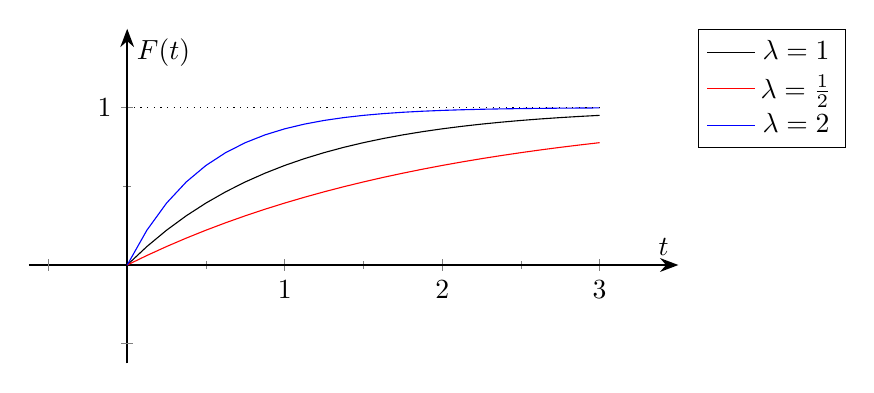
\begin{tikzpicture}[]
		\begin{axis}[
		legend pos = outer north east,
		x = 2cm,
		y = 2cm,
		axis lines=middle,
		axis line style={-Stealth,thick},
		xmin=-0.625,xmax=3.5,ymin=-0.625,ymax=1.5,
		xtick={0,1,2,3},
		ytick={0,1},
		extra x ticks={-0.5},
		extra y ticks={-0.5},
		extra x tick style={xticklabel=\empty},
		extra y tick style={yticklabel=\empty},
		xtick distance=1,
		ytick distance=1,
		xlabel=$t$,
		ylabel=$F(t)$,
		%title={Wonderful plot},
		minor tick num= 1,
		%grid=both,
		grid style={thin,densely dotted,black!20}]
		%\addplot [Latex-Latex,domain=-5:3,samples=2] {x*2/3} node[right]{$a$};
		\addplot [domain = 0:3] {1-e^(-x)}; \addlegendentry{$\lambda = 1$};
		\addplot [domain = 0:3, color = red] {1-e^(-x*0.5)}; \addlegendentry{$\lambda = \frac{1}{2}$};
		\addplot [domain = 0:3, color = blue] {1-e^(-x*2)}; \addlegendentry{$\lambda = 2$};
		\addplot [dotted] coordinates{(0,1) (3,1)};
		\end{axis}
		\end{tikzpicture}
	\end{center}
	Man nennt das Ma\ss{} auch \textbf{$\operatorname{Exp}(\lambda)$}. In der Graphik ist $\operatorname{Exp}(\lambda)$ f\"ur drei verschiedene $\lambda$ geplotted. 
\end{beispiel}

	

\begin{deff}\label{as}
\link{https://www.youtube.com/watch?v=8pGCVx1Z7fk&list=PLy5qRKPWp6SBwfc1kn-b66cWc84cOgvqZ&index=7&t=3805s}
	Ist $f \! : \mathbb{R} \rightarrow [0,\infty)$ integrierbar mit $ \int_{\mathbb{R}} f(x) \text{d}x = 1$,  dann heißt $f$ \textbf{Dichtefunktion} der Verteilungsfunktion 
	\begin{align}\label{kk}
		F(t) = \int\limits_{-\infty}^{t} f(x) \mathrm{d}x,\quad t\in\R.
	\end{align}	
	Beachte: Solch eine Integralfunktion $F$ erf\"ullt automatisch die Eigenschaften einer Verteilungsfunktion (siehe gro\ss e \"Ubung)! Ist umgekehrt $F$ von der Form \eqref{kk}, so heißt $f$ \textbf{Dichte} von $F$. Verteilungsfunktionen mit Dichten nennt man auch \textbf{absolutstetig}, Wahrscheinlichkeitsma\ss e auf $\mathcal B(\R)$ mit absolutstetiger Verteilungsfunktion nennt man \textbf{absolutstetige Ma\ss e}.
\end{deff}
Zwei Beispiele haben wir schon gesehen: $\mathcal U([a,b])$ und $\operatorname{Exp}(\lambda)$ haben beide absolutstetige Verteilungsfunktionen. Die zugeh\"origen Dichten berechnet ihr in den \"Ubungsaufgaben. Aber wie findet man die Dichten von absolutstetigen Verteilungsfunktionen? Ableiten! Das ist, zumindest f\"ur stetige Dichten, der Hauptsatz der Integral- und Differentialrechnung. Probiert das bei den zwei Beispielen mal aus. Ableiten ohne nachzudenken erlaubt es die Dichte $f$ zu erraten, wenn man dann durch Integrieren $F(t)=\int_{-\infty}^t f(x)\mathrm{d}x$ nachrechnen kann, so ist $f$ eine Dichte von $F$. Warum es praktisch ist eine absolutstetige Verteilungsfunktion zu haben, wird zum Beispiel in Diskussion \ref{diskussion} klarer. Man kann direkt wichtige Eigenschaften des Ma\ss es $\mathbb P_F$ aus der Dichte $f$ ablesen.


\begin{beispiel}
\link{https://www.youtube.com/watch?v=8pGCVx1Z7fk&list=PLy5qRKPWp6SBwfc1kn-b66cWc84cOgvqZ&index=7&t=4100s}
	Die sch\"onste Anwendung von Polarkoordinaten und Fubini (siehe Analysis 2) ist die Berechnung des Integrals $\int_\R e^{-\frac{x^2}{x}}dx=\sqrt{2\pi}$. Damit ist $f(x)=\frac{1}{\sqrt{2\pi}} e^{-\frac{x^2}{2}}$ eine Dichtefunktion. Man nennt die zugeh\"orige Verteilungsfunktion

	\[ F(t) = \int\limits_{-\infty}^{t} \frac{1}{\sqrt{2\pi}} e^{-\frac{x^2}{2}} \text{d}x,\quad t\in\R,\]  Verteilungsfunktion der \textbf{(standard) Normalverteilung}. Das Ma\ss{} $\mathbb P_F$ nennt man dann auch (standard) normalverteilt und man schreibt $\mathbb{P}_F\sim$ \textbf{ $\cN(0,1)$}. In der gro\ss en \"Ubung wird diskutiert, dass f\"ur $\mu\in\R$ und $\sigma^2\geq 0$ auch $f(x)=\frac{1}{\sqrt{2\pi\sigma^2}} e^{-\frac{(x-\mu)^2}{2\sigma^2}}$ eine Dichtefunktion ist. Die zugeh\"orige Verteilung nennt man auch normalverteilt und schreibt $\mathcal N(\mu, \sigma^2)$. 
\begin{center}
		\begin{tikzpicture}[]
		\begin{axis}[
		legend pos = outer north east,
		x = 2cm,
		y = 2cm,
		axis lines=middle,
		axis line style={-Stealth,thick},
		xmin=-2,xmax=2.5,ymin=-0.625,ymax=1,
		xtick={-2,-1,0,1,2},
		ytick={0,0.5},
		extra x ticks={-0.5},
		extra y ticks={-0.5},
		extra x tick style={xticklabel=\empty},
		extra y tick style={yticklabel=\empty},
		xticklabel=\empty,
		yticklabel=\empty,
		xtick distance=1,
		ytick distance=1,
		xlabel=$x$,
		ylabel=$f(x)$,
		%title={Wonderful plot},
		minor tick num= 1,
		%grid=both,
		grid style={thin,densely dotted,black!20}]
		%\addplot [Latex-Latex,domain=-5:3,samples=2] {x*2/3} node[right]{$a$};
		%\addplot [domain = -0.5:3] {exp(-(x-1)^2 / (2*0.2)) / (sqrt(2*pi*0.2))};
		\addplot [name path = A, domain = -2:3, color = blue, smooth] {gauss(1,0.45)};\addlegendentry{$\mu = 2, \sigma^2=\frac 1 2$};
		\addplot [name path = A, domain = -2:3, color = red, smooth] {gauss(0,0.8)};\addlegendentry{$\mu = 0, \sigma^2=1$};
		%\addlegendentry{$f$};
%		\addlegendentry{\empty};
%		\path [name path=B] (\pgfkeysvalueof{/pgfplots/xmin},0) -- (\pgfkeysvalueof{/pgfplots/xmax},0);
	%	\addplot [blue, fill opacity=0.4] fill between [
	%	of=A and B,
	%	soft clip={domain=0.75:1.25},
	%	]; 
	%	\addplot [red, fill opacity=0.4] fill between [
	%	of=A and B,
	%	soft clip={domain=1.75:2.5},
	%	]; 
%		\legend{,viel Masse,wenig Masse};
		\end{axis}
		\end{tikzpicture}
	\end{center}		
	
	
	Die Bedeutung von $\mu$ und $\sigma^2$ diskutierten wir sp\"ater. Warnung: Warum schreiben wir nur eine Formel f\"ur die Dichte $f$, jedoch nicht f\"ur die Verteilungsfunktion $F$ hin? Es gibt einfach keine Formel f\"ur das Integral $\int_{-\infty}^t e^{-x^2/2}dx$! Aufgrund der Form der Kurve spricht man auch von der Glockenkurve und weil diese von Gau\ss{} entdeckt wurde, von der Gausschen Glockenkurve.
	\end{beispiel}

Das Gegenst\"uck zu absolutstetigen Verteilungen sind sogenannte diskrete Verteilungen:	
\begin{beispiel}\label{Poi}
\link{https://www.youtube.com/watch?v=8pGCVx1Z7fk&list=PLy5qRKPWp6SBwfc1kn-b66cWc84cOgvqZ&index=7&t=4642s}
	Für $a_1,...,a_N \in \mathbb{R}$, $N\in \N$ oder $N=+\infty$, mit $p_1,...,p_N \geq 0$ und $\sum\limits_{k= 1}^{N} p_k= 1$ ist \[F(t):= \sum\limits_{k= 1}^{N} p_k \mathbf{1}_{[a_k, \infty)}(t)=\sum_{a_k\leq t} p_k, \quad t\in\R, \] eine Verteilungsfunktion. Die zugeh\"origen Ma\ss e $\mathbb P_F$ werden \textbf{(endliche) diskrete Verteilungen} genannt. In den \"Ubungen zeigt ihr, dass die Ma\ss e im diskreten Fall ganz einfach angegeben werden k\"onnen, es sind Mischungen aus Dirac-Ma\ss en an den Stellen $a_1,...,a_N$: $$\mathbb P_F=\sum_{k=1}^N p_k\delta_{a_k}.$$ Wie zeigt man das? Einfach die Menge $(-\infty,t]$ in das Ma\ss{} einsetzen, das gibt das gew\"unschte $F$.
	\begin{center}	
		\begin{tikzpicture}[]
		\begin{axis}[
		x = 2cm,
		y = 2cm,
		axis lines=middle,
		axis line style={-Stealth,thick},
		xmin=-1.6,xmax=2.8,ymin=-0.625,ymax=1.5,
		xtick={0},
		ytick={0,1},
		extra x ticks={-0.5},
		extra y ticks={-0.5},
		extra x tick style={xticklabel=\empty},
		extra y tick style={yticklabel=\empty},
		xtick distance=1,
		ytick distance=1,
		xlabel=$t$,
		ylabel=$F(t)$,
		%title={Wonderful plot},
		minor tick num= 1,
		%grid=both,
		grid style={thin,densely dotted,black!20}]
		%\addplot [Latex-Latex,domain=-5:3,samples=2] {x*2/3} node[right]{$a$};
		\addplot [domain = -1:-0.5] {0.3};
		\addplot [domain = -0.5:0.2] {0.5};	 
		\addplot [domain = 0.2:2] {0.7};
		\addplot [domain = 2:3] {1};
		\addplot [only marks] coordinates{(-0.5,0.5)(-1,0.3)(0.2,0.7) (2,1)};
		\addplot [dotted] coordinates{(-1,0.3) (-1,0)};
		\addplot [dotted] coordinates{(-0.5,0.5) (-0.5,0.3)};
		\addplot [dotted] coordinates{(0.2,0.5) (0.2,0.7)};
		\addplot [dotted] coordinates{(2,0.7) (2,1)};
				\addplot [dotted] coordinates{(-1.6,1) (2,1)};
		\end{axis}
		\end{tikzpicture}
\end{center}
	\link{https://www.youtube.com/watch?v=8pGCVx1Z7fk&list=PLy5qRKPWp6SBwfc1kn-b66cWc84cOgvqZ&index=7&t=4963s}
	Ganz konkret heißt $\mathbb{P}_F$ für $a_k=k$ und $p_k = e^{-\lambda} \frac{\lambda^k}{k!}$, $k \in \N$, \textbf{Poissonverteilung mit Parameter $\lambda>0$} auf $\cB(\mathbb{R})$. Beachte: Weil wir die Poissonverteilung bereits auf $\mathcal P(\N)$ definiert haben gibt es eine gewisse Doppeldeutigkeit. Mit der Diskussion der n\"achsten Vorlesung wird aber klar, dass beide Ma\ss e das gleiche beschreiben, n\"amlich die Verteilung einer Einheit Masse auf $\N$ mit den Wahrscheinlichkeiten $p_k$ f\"ur die die nat\"urliche Zahl $k$. Die Poissonverteilung mit Parameter $\lambda$ wird auch als \textbf{Poi$(\lambda)$} genannt.
	\begin{center}	
		\begin{tikzpicture}[]
		\begin{axis}[
		x = 2cm,
		y = 2cm,
		axis lines=middle,
		axis line style={-Stealth,thick},
		xmin=-0.4,xmax=5,ymin=-0.525,ymax=1.5,
		xtick={0,1,2,3,4},
		ytick={0,1},
		extra x ticks={-0.5},
		extra y ticks={-0.5},
		extra x tick style={xticklabel=\empty},
		extra y tick style={yticklabel=\empty},
		xtick distance=1,
		ytick distance=1,
		xlabel=$t$,
		ylabel=$F(t)$,
		%title={Wonderful plot},
		minor tick num= 1,
		%grid=both,
		grid style={thin,densely dotted,black!20}]
		%\addplot [Latex-Latex,domain=-5:3,samples=2] {x*2/3} node[right]{$a$};
		\addplot [domain = 0:1] {0.26};
		\addplot [domain = 1:2] {0.5};	 
		\addplot [domain = 2:3] {0.7};
		\addplot [domain =3:4] {0.82};
		\addplot [domain =4:5] {0.93};
		\addplot [only marks] coordinates{(0,0.26)(1,0.5)(2,0.7) (3,0.82) (4,0.93)};
		\addplot [dotted] coordinates{(1,0.26) (1,0.5)};
		\addplot [dotted] coordinates{(2,0.5) (2,0.7)};
		\addplot [dotted] coordinates{(3,0.7) (3,0.82)};
		\addplot [dotted] coordinates{(4,0.82) (4,0.93)};
		\addplot [dotted] coordinates{(-0.6,1) (6,1)};
		\end{axis}
		\end{tikzpicture}
\end{center}
	
	
	
	
\end{beispiel}


\marginpar{\textcolor{red}{Vorlesung 7}}
Manche werden sich fragen, wo denn jetzt die Stochastik geblieben ist. Wir haben schlie\ss lich gerade Begriffe der Stochastik benutzt, z. B. den Begriff der Uniformverteilung, auch die Gau\ss sche Glockenfunktion ist bereits aufgetaucht, \"uber zuf\"allige Experimente haben wir aber schon l\"anger nicht gesprochen. Als konkrete Motivation zur Nutzung der abstrakten Theorie zur Modellierung zuf\"alliger Experimente, schauen wir uns das uniforme Ziehen aus $[0,1]$ an.

\begin{disc}
\link{https://www.youtube.com/watch?v=ZQeE6Nv1k_0&t=80s} \textbf{[Stochastische Modellierung, Nr. 2]}
	Das Modellieren von endlich vielen Möglichkeiten ist relativ einfach, siehe Diskussion \ref{N1}. Man kommt recht nat\"urlich auf die Eigenschaften der $\sigma$-Algebra und des Ma\ss es. Zur Erinnerung war das gleichverteilte Ziehen aus einer endlichen Menge modelliert durch den endlichen Zustandsraum $\Omega$ (=M\"oglichkeiten zum Ziehen), $\cA = \cP(\Omega)$ und der diskreten Gleicherverteilung $\mathbb{P}(A) = \frac{\# A}{\# \Omega}$.\\ Das Modellieren von Experimenten mit unendlich vielen Möglichkeiten ist dagegen schwieriger. Wie modelliert man zum Beispiel das Ziehen aus dem Intervall $[0,1]$, sodass kein Bereich von $[0,1]$ bevorteilt wird? Wenn wir beobachten wollen, ob eine feste Zahl gezogen wurde oder nicht, m\"ussen die einelementigen Mengen $\{t\}$ in der $\sigma$-Algebra sein. Wenn kein Element bevorzugt werden soll, also $\mathbb P(\{t\})$ f\"ur alle $t$ gleich sein soll, f\"uhrt die Unendlichkeit automatisch zu $\mathbb P(\{t\})=0$ f\"ur alle $t\in [0,1]$. Warum das? Wenn man irgendeine Folge $(a_n)$ unterschiedlicher Zahlen in $[0,1]$ w\"ahlt, z. B. $a_n=\frac 1 n$, und $\mathbb P(\{t\})=:c$ f\"ur alle $t$ setzt, so gilt wegen der $\sigma$-Addititivit\"at von Ma\ss en
	\begin{align*}
		1\geq \mathbb P\big(\bigcupdot_{k=1}^\infty \{a_k\}\big) =\sum_{k=1}^\infty \mathbb P(\{a_k\})=\sum_{k=1}^\infty c,
	\end{align*}
	also $c=0$. Hier sehen wir deutlich den Unterschied zur Gleichverteilung auf endlichen Mengen, die einfache Definition durch Einpunktmengen f\"uhrt zu nichts! Im Gegensatz zum endlichen Fall legen wir f\"ur gleichverteilten Zufall in $[0,1]$ jetzt fest, dass die Wahrscheinlichkeit von Teilintervallen von $[0,1]$ nur von der L\"ange abh\"angen soll. Das f\"uhrt zur Forderung $\mathbb P((a,b])=b-a=F(b)-F(a)$ f\"ur $a<b$ aus $[0,1]$, wobei $F$ die Verteilungsfunktion aus Beispiel \ref{Gl} ist. Da wir als mathematisches Modell des zuf\"alligen Ziehens eine $\sigma$-Algebra und ein Ma\ss{} haben wollen, w\"ahlen wir nun die kleinste $\sigma$-Algebra die all diese Intervalle enth\"alt (die Borel-$\sigma$-Algebra) und darauf ein Ma\ss, das den Intervallen die geforderten Wahrscheinlichkeiten gibt. Aufgrund des Fortsetzungssatzes gibt es so ein Ma\ss, das ist gerade $\mathcal U([0,1])$.
\end{disc}

Hoffentlich ist jetzt einsichtig, warum die Modellierung von komplizierten reellen zuf\"alligen Experimenten mit der Borel-$\sigma$-Algebra Sinn macht. Eine Frage bleibt aber noch: Warum nehmen wir nicht einfach die ganze Potenzmenge auf $\R$ als Modell, so wie beim zuf\"alligen Ziehen in endlichen Mengen?
\begin{bem}
\link{https://www.youtube.com/watch?v=ZQeE6Nv1k_0&t=905s}
	\begin{enumerate}[label=(\roman*)]
		\item $\cB(\mathbb{R})$ funktioniert wunderbar! Insbesondere weil wir sehr handliche Erzeuger haben (z. B. verschiedene Arten von Intervallen) und deshalb aufgrund der bewiesenen Theoreme (fast) nur mit Intervallen arbeiten m\"ussen.
				\item $\cP(\mathbb{R})$ ist zu groß, \mbox{z. B.} das Lebesgue-Maß oder die Normalverteilung kann zwar auf $\cB(\mathbb{R})$, aber nicht auf $\cP(\mathbb{R})$ definiert werden ($\rightsquigarrow$ Vitali-Menge). Es gilt tats\"achlich $\cB(\mathbb{R}) \subsetneq \cP(\mathbb{R})$, ganz einfache Beispiele f\"ur nicht Borel-messbare Mengen gibt es aber nicht.
	\end{enumerate}
\end{bem}

Die n\"achste Runde der Modellierung zuf\"alliger Experimente findet erst in ein paar Wochen statt. Bis dahin k\"onnt ihr die Ideen sacken lassen und euch wieder an der abstrakten Theorie erfreuen.\smallskip




Das Umschalten im Kopf von Verteilungsfunktionen auf Ma\ss e ist anfangs extrem schwierig. Wir wissen zwar abstrakt, dass es f\"ur jede Verteilungsfunktion genau ein Ma\ss{} auf $\mathcal B(\R)$ gibt und andersrum f\"ur jedes Ma\ss{} eine eindeutige Verteilungsfunktion, aber was bedeutet das konkret? Das versteht man am besten, wenn man Eigenschaften von $F$ in Eigenschaften von $\mathbb P_F$ \"ubersetzt:

\begin{disc}\label{diskussion}
\link{https://www.youtube.com/watch?v=ZQeE6Nv1k_0&t=1130s}
Wir starten mit einer nicht sehr rigorosen aber dennoch hilfreichen Interpretation:
\begin{center} \glqq$F$ beschreibt, wie durch $\mathbb P_F$ eine Einheit Zufall auf $\mathbb{R}$ verteilt wird.\grqq \end{center}
Dazu sei $F(b) - F(a)$ der Anteil des gesamten Zufalls ($F(b)-F(a)$ ist immer zwischen $0$ und $1$), der in $(a,b]$ gelandet ist. Man spricht auch statt \enquote{Anteil} von der \enquote{Masse} Zufall in $(a,b]$.\smallskip

Wir schauen uns jetzt an, was drei Eigenschaften von $F$ (stetig, konstant, stark wachsend) f\"ur die Verteilung der Masse bedeuten.\smallskip

\textbf{Stetigkeit vs. Spr\"unge:} Zun\"achst berechnen wir die Masse einer Einpunktmenge $\{t\}$ aus den bekannten Eigenschaften von Ma\ss en und Verteilungsfunktionen. Wie immer versuchen wir die gesuchte Menge durch Mengen der Form $(a,b]$ auszudr\"ucken, weil wir f\"ur diese Mengen eine Verbindung zwischen $F$ und $\mathbb P_F$ haben:
	 \begin{align*}
			\mathbb{P}_F(\{ t \}) &= 
			\mathbb{P}_F \Big(\bigcap\limits_{n = 1}^{\infty} \Big(t - \frac{1}{n}, t\Big] \Big) \\
			\overset{\text{Stet. Ma\ss e}}&{=} \lim\limits_{n \to \infty} \mathbb{P}_F\Big(\Big(t - \frac{1}{n}, t\Big]\Big) \\
			\overset{\text{Def. }\mathbb P_F}&{=} \lim\limits_{n \to \infty} \Big(F(t) - F\Big(t - \frac{1}{n}\Big)\Big)\\
			&= F(t) - \lim\limits_{n \to \infty} F\Big(t - \frac{1}{n}\Big) = F(t) - F(t-),
		\end{align*}
		wobei $F(t-):=\lim_{s\uparrow t} F(s)$ der Linksgrenzwert aus der Analysis ist. Konsequenz: Ist $F$ stetig in $t$, so hat die Einpunktmenge $\{t\}$ keine Masse. Hierzu beachte man, dass $F$ an jeder Stelle rechtsstetig ist, die Stetigkeit somit \"aquivalent zu $F(t)=F(t-)$ ist.
		Insbesondere haben \underline{alle} einpunktigen Mengen keine Masse, sofern $F$ eine stetige Funktion ist (\mbox{z. B.} bei \textbf{$\mathcal U([a,b])$, $\operatorname{Exp}(\lambda)$, $\cN(\mu, \sigma^2)$)}. Klingt komisch, oder? Ist es aber nicht. Hier sehen wir, warum Ma\ss e erst auf \"uberabz\"ahlbaren Mengen wirklich spannend werden: \[ \mathbb{P}_F((a,b]) = \mathbb{P}_F \Big( \bigcupdot\limits_{t \in (a,b]} \{t\} \Big) \neq \sum\limits_{t \in (a,b]} \mathbb{P}_F(\{t\}),\] weil $\sigma$-Additivität nur f\"ur Vereinigungen abz\"ahlbar vieler Mengen gilt. Was sollte die \"uberabz\"ahlbare Summe auf der rechten Seite auch bedeuten?\smallskip
		
\textbf{$F$ konstant:} \"Uberlegen wir nun, was es f\"ur $\mathbb P_F$ bedeutet, wenn $F$ auf einem Intervall konstant ist. Schauen wir dazu zun\"achst ein Beispiel an. Betrachten wir folgende einfache Verteilungsfunktion
\begin{center}	
		\begin{tikzpicture}[]
		\begin{axis}[
		x = 2cm,
		y = 2cm,
		axis lines=middle,
		axis line style={-Stealth,thick},
		xmin=-0.625,xmax=3,ymin=-0.625,ymax=1.5,
		xtick={0,1,2},
		ytick={0,1},
		extra x ticks={-0.5},
		extra y ticks={-0.5},
		extra x tick style={xticklabel=\empty},
		extra y tick style={yticklabel=\empty},
		xtick distance=1,
		ytick distance=1,
		xlabel=$t$,
		ylabel=$F(t)$,
		%title={Wonderful plot},
		minor tick num= 1,
		%grid=both,
		grid style={thin,densely dotted,black!20}]
		%\addplot [Latex-Latex,domain=-5:3,samples=2] {x*2/3} node[right]{$a$};
		\addplot [domain = 1:2] {1/2}; 
		\addplot [domain = 2:3] {1};
				\addplot [dotted] coordinates{(-0.625,1) (2,1)};
		\addplot [only marks] coordinates{(1,0.5) (2,1)};
		\addplot [dotted] coordinates{(1,0.5) (1,0)};
		\addplot [dotted] coordinates{(2,0.5) (2,1)};
%		\addplot [dotted] coordinates{(3,0) (3,1)};
		\end{axis}
		\end{tikzpicture}
\end{center}
	aus der Klasse der diskreten Verteilungen. Nach der Diskussion zur Stetigkeit wissen wir, dass das zugeh\"orige Ma\ss{} $\mathbb P_F$ folgendes erf\"ullt: $\mathbb P_F(\{1\})=	\mathbb P_F(\{2\})=\frac{1}{2}.$ Wegen der $\sigma$-Additivit\"at folgt nat\"urlich (es gibt insgesamt nur eine Einheit Zufall zu verteilen), dass $\mathbb P_F(A)=0$ f\"ur alle Borelmengen $A$ mit $1,2\notin A$. Das Ma\ss{} $\mathbb P_F$ hat also keine Masse au\ss erhalb der Menge $\{1,2\}$. Schauen wir uns $F$ an, so sehen wir also, dass $\mathbb P_F$ keine Masse in den konstanten Bereichen hat. F\"ur Intervalle $(a,b]$ folgt das allgemein nat\"urlich aus $\mathbb P_F((a,b])=F(b)-F(a)$ was gerade $0$ ist, wenn $F$ zwischen $a$ und $b$ konstant ist:
	\begin{center}
		\glqq $\mathbb{P}_F$ hat keine Masse dort, wo $F$ konstant ist.\grqq
	\end{center}

	Wenn wir die Beobachtung auf $\operatorname{Poi}(\lambda)$ aus Beispiel \ref{Poi} anwenden, so sehen wir, dass das zugeh\"ogige Ma\ss{} $\mathbb P_F$ nur Masse auf $\N$ hat. Damit kann man ein $\operatorname{Poi}(\lambda)$-verteilte Ma\ss{} auf $\mathcal B(\R)$ mit der Definition aus Beispiel \ref{Poi1} identifizieren, wir verteilen eine Einheit Zufall jeweils auf $\N$ (einmal wird die Einheit Zufall direkt auf $\N$ verteilt, einmal auf $\N$ als Teilmenge von $\R$).
	
	\textbf{$F$ stark wachsend:} Wir wissen nun wieviel Masse an Sprungstellen liegt und auch, dass keine Masse in konstanten Bereichen liegt. Fragt sich also, wo die Masse sonst noch zu finden ist: 
	\begin{center}
		\glqq $\mathbb{P}_F$ hat viel Masse dort, wo $F$ am st\"arksten wächst.\grqq
	\end{center}
	Formell folgt das nat\"urlich aus $\mathbb P_F((a,b])=F(b)-F(a)$ weil dann auf ein kleines Intervall $(a,b]$ viel Masse verteilt wird, wenn $F(b)$ deutlich gr\"o\ss er als $F(a)$. Ist $a$ nah an $b$, so bedeutet das nat\"urlich, dass $F$ dort stark w\"achst. Schauen wir uns wieder ein passendes Beispiel an, die Exponentialverteilung $\operatorname{Exp}(\lambda)$ f\"ur verschiedene $\lambda>0$. Am Bildchen in Beispiel \ref{Exp} ist zu erkennen, dass viel Masse nah bei der $0$ liegt wenn $\lambda$ gro\ss{} ist, die Verteilungsfunktion bei $0$ also steil ist. Nat\"urlich sehen wir das auch formell aus der Verteilungsfunktion weil f\"ur alle $\varepsilon>0$
\begin{align*}
	\mathbb P_F((0,\varepsilon])=F(\varepsilon)-F(0)= (1-e^{-\lambda \varepsilon})-(1-e^{-\lambda 0})=1-e^{-\lambda \varepsilon},
\end{align*}
	was monoton wachsend in $\lambda$ ist.\smallskip
	
	\textbf{Der Fall mit Dichten:} Die obige Diskussion k\"onnen wir f\"ur Verteilungsfunktionen mit Dichten noch konkretisieren. Sei dazu $F$ eine Verteilungsfunktion mit Dichte $f$, also $F(t) = \int\limits_{-\infty}^{t}  f(x) \mathrm{d}x$. Weil $F$ stetig ist, haben alle einpunktigen Mengen keine Masse. Aber wie k\"onnen wir an $f$ direkt sehen, wo die Masse verteilt ist? Ist $f$ stetig, so folgt aus dem Hauptsatz der Analysis $F'(t)=f(t)$ f\"ur alle $t\in \R$. Folglich impliziert ein an der Stelle $t$ gro\ss es $f$ ein in $t$ stark wachsendes $F$ und damit viel Masse um $t$. Andersrum impliziert ein an der Stelle $t$ kleines $f$ ein in $t$ wenig wachsendes $F$ und damit wenig Masse um $t$. Im Extremfall impliziert nat\"urlich $f=0$ in $(a,b]$ auch $F$ konstant in $(a,b]$ und damit wird keine Masse auf $(a,b]$ verteilt. Wir merken uns grob 
	\begin{center}
		\glqq Hat $F$ eine Dichte, so ist viel Masse dort, wo $f$ gro\ss{} ist.\grqq
	\end{center}	
	 Die n\"utzlichste Interpretation ist durch den Fl\"acheninhalt zwischen Graphen von $f$ und der $x$-Achse gegeben. Wegen	
		\begin{align*}
			\mathbb{P}_F((a,b]) 
			= F(b)-F(a)
			= \int\limits_{-\infty}^{b} f(x) \mathrm{d}x - \int\limits_{-\infty}^{a} f(x) \mathrm{d}x 
			=\int\limits_{a}^{b} f(x) \mathrm{d}x,
		\end{align*}
		ist die Masse in $(a,b]$ gerade die Fl\"ache unter $f$ zwischen $a$ und $b$. Dazu ist zu beachten, dass nach Annahme die Gesamtfl\"ache zwischen Graphen und $x$-Achse $1$ ist. 		
		
		In folgendem Beispiel ist die Dichte von $\mathcal N(2, 1)$ geplottet:
	\begin{center}
		\begin{tikzpicture}[]\label{c}
		\begin{axis}[
		legend pos = outer north east,
		x = 2cm,
		y = 2cm,
		axis lines=middle,
		axis line style={-Stealth,thick},
		xmin=-0.625,xmax=3.25,ymin=-0.625,ymax=1.5,
		xtick={0,1,2,3},
		ytick={0,1},
		extra x ticks={-0.5},
		extra y ticks={-0.5},
		extra x tick style={xticklabel=\empty},
		extra y tick style={yticklabel=\empty},
		xticklabel=\empty,
		yticklabel=\empty,
		xtick distance=1,
		ytick distance=1,
		xlabel=$t$,
		ylabel=$f(t)$,
		%title={Wonderful plot},
		minor tick num= 1,
		%grid=both,
		grid style={thin,densely dotted,black!20}]
		%\addplot [Latex-Latex,domain=-5:3,samples=2] {x*2/3} node[right]{$a$};
		%\addplot [domain = -0.5:3] {exp(-(x-1)^2 / (2*0.2)) / (sqrt(2*pi*0.2))};
		\addplot [name path = A, domain = -0.75:3, smooth] {gauss(1,0.45)};
		%\addlegendentry{$f$};
		\addlegendentry{\empty};
		\path [name path=B] (\pgfkeysvalueof{/pgfplots/xmin},0) -- (\pgfkeysvalueof{/pgfplots/xmax},0);
		\addplot [green, fill opacity=0.4] fill between [
		of=A and B,
		soft clip={domain=0.75:1.25},
		]; 
		\addplot [red, fill opacity=0.4] fill between [
		of=A and B,
		soft clip={domain=1.75:2.5},
		]; 
		\legend{,viel Masse,wenig Masse};
		\end{axis}
		\end{tikzpicture}
	\end{center}	
	Wir sehen also, dass viel Masse des Ma\ss es $\mathcal N(2,1)$ um die $2$ herum verteilt ist und sehr wenig Masse weit weg von der $2$ verteilt ist. Der gr\"une Bereich ist gerade so gew\"ahlt, dass dieser Fl\"acheninhalt $\frac 1 3$ ist. Ein Drittel der Masse von $\mathcal N(2,1)$ liegt also im Schnittbereich des gr\"unen Bereichs mit der $x$-Achse, sehr nah an der $2$. Man sagt, die Verteilung ist um $2$ konzentriert. Wenn wir zwei verschiedene Normalverteilungen vergleichen, sieht es wie im folgenden Beispiel aus:
		\begin{center}
		\begin{tikzpicture}[]
		\begin{axis}[
		legend pos = outer north east,
		x = 2cm,
		y = 2cm,
		axis lines=middle,
		axis line style={-Stealth,thick},
		xmin=-2,xmax=3,ymin=-0.625,ymax=1,
		xtick={-2,-1,0,1,2,3},
		ytick={0,1},
		extra x ticks={-0.5},
		extra y ticks={-0.5},
		extra x tick style={xticklabel=\empty},
		extra y tick style={yticklabel=\empty},
		xticklabel=\empty,
		yticklabel=\empty,
		xtick distance=1,
		ytick distance=1,
		xlabel=$t$,
		ylabel=$f(t)$,
		%title={Wonderful plot},
		minor tick num= 1,
		%grid=both,
		grid style={thin,densely dotted,black!20}]
		%\addplot [Latex-Latex,domain=-5:3,samples=2] {x*2/3} node[right]{$a$};
		%\addplot [domain = -0.5:3] {exp(-(x-1)^2 / (2*0.2)) / (sqrt(2*pi*0.2))};
		\addplot [name path = B, domain = -2:3, color = blue, smooth] {gauss(1,0.45)};\addlegendentry{$\mu = 2, \sigma^2=\frac 1 2$};
		\addplot [name path = A, domain = -2:3, color = red, smooth] {gauss(0,0.8)};\addlegendentry{$\mu = 0, \sigma^2=1$};
		\path [name path=C] (\pgfkeysvalueof{/pgfplots/xmin},0) -- (\pgfkeysvalueof{/pgfplots/xmax},0);
		%\addlegendentry{$f$};
%		\addlegendentry{\empty};
	
		\addplot [green, fill opacity=0.4] fill between [
		of=A and C,
		soft clip={domain=-0.4:0.4},
		]; 
		
		\addplot [green, fill opacity=0.4] fill between [
		of=B and C,
		soft clip={domain=0.75:1.25},
		]; 
		

	%	\addplot [red, fill opacity=0.4] fill between [
	%	of=A and B,
	%	soft clip={domain=1.75:2.5},
	%	]; 
%		\legend{,viel Masse,wenig Masse};
		\end{axis}
		\end{tikzpicture}
		\end{center}
		Der Inhalt der gr\"unen Fl\"achen ist wieder $\frac 1 3$, die zugeh\"origen normalverteilten Ma\ss e auf $\mathcal B(\R)$ haben deshalb Masse $\frac 1 3$ im jeweiligen Schnittbereich mit der $x$-Achse. Wir sehen schon an dem Bild, dass niedrigeres $\sigma$ daf\"ur sorgt, dass die Verteilung mehr Masse nah an $\mu$ hat. Darauf gehen wir in ein paar Wochen noch viel ausf\"uhrlicher ein.
\end{disc}



\chapter{Abbildungen zwischen messbaren Räumen}
\marginpar{\textcolor{red}{Vorlesung 8}}
Bevor wir messbare Abbildungen definieren, erinnern wir kurz an bereits bekannte Konzepte in der Mathematik. Wir betrachten immer Objekte und Abbildungen zwischen Objekten, die auf eine gewisse Art \glqq nat\"urlich\grqq{} (strukturerhaltend) sind:
\begin{center}
\bgroup
\def\arraystretch{1}
 \begin{tabular}{c|c}
	Mengen& Abbildungen\\
	Gruppen&Homomorphismen\\ 
	Vektorräume&Lineare Abbildungen\\
	Metrische Räume& stetige Abbildungen\\
\end{tabular}
\egroup
\end{center}
Passend dazu diskutieren wir jetzt die strukturerhaltenden Abbildungen zwischen messbaren R\"aumen, sogenannte messbare Abbildungen.
\section{Messbare Abbildungen}



\begin{deff}
\link{https://www.youtube.com/watch?v=Pj5TaNiE05c&list=PLy5qRKPWp6SBwfc1kn-b66cWc84cOgvqZ&index=9&t=229s}
	Seien $(\Omega, \cA)$, $(\Omega', \cA')$ messbare Räume und $f \! : \Omega \rightarrow \Omega'$. $f$ heißt \mbox{\textbf{messbar}}, falls Urbilder messbarer Mengen messbar sind; in Formeln \[A' \in \cA' \,\Rightarrow\, f^{-1} (A') \in \cA.\]
\end{deff}
	Es gibt verschiedene Notationen f\"ur messbare Abbildungen. Man nutzt synonym 
	\begin{itemize}
		\item $f:\Omega \to \Omega'$ ist $(\mathcal A, \mathcal A')$-messbar,
		\item $f: (\Omega, \mathcal A)\to (\Omega',\mathcal A')$ ist messbar,
				\item $f:\Omega\to \Omega'$ ist messbar bez\"uglich $\mathcal A$ und $\mathcal A'$.
	\end{itemize}
	Genau wie Stetigkeit zwischen metrischen R\"aumen von den gew\"ahlten Metriken abh\"angt, h\"angt auch die Messbarkeit von den gew\"ahlten $\sigma$-Algebren ab. Wenn klar ist, welche $\sigma$-Algebren gew\"ahlt sind, redet man trotzdem einfach nur von messbaren Abbildungen.
\begin{bem}
\link{https://www.youtube.com/watch?v=Pj5TaNiE05c&list=PLy5qRKPWp6SBwfc1kn-b66cWc84cOgvqZ&index=9&t=520s}
	Die Definition der Messbarkeit ist analog zur Stetigkeit zwischen metrischen Räumen, dabei werden messbare Mengen durch offene Mengen ersetzt.
\end{bem}

\begin{deff}
\link{https://www.youtube.com/watch?v=Pj5TaNiE05c&list=PLy5qRKPWp6SBwfc1kn-b66cWc84cOgvqZ&index=9&t=588s}
	Ist $ (\Omega', \cA') = (\mathbb{R}, \cB(\mathbb{R})) $, dann nennt man eine messbare Abbildung auch \textbf{Zufallsvariable} und schreibt $X$ statt $f$.
\end{deff}
Wie bei der Konstruktion von Ma\ss en haben wir das Problem, dass wir alle messbaren Mengen testen m\"ussen. Das ist gerade bei der Borel-$\sigma$-Algebra unm\"oglich, wir kennen die Mengen nicht alle. Zum Gl\"uck ist es wie im Kapitel zuvor, es reicht einen Erzeuger zu betrachten:
\begin{prop}\label{S2}
\link{https://www.youtube.com/watch?v=Pj5TaNiE05c&list=PLy5qRKPWp6SBwfc1kn-b66cWc84cOgvqZ&index=9&t=706s}
	Ist $\cE'$ ein Erzeuger von $\cA'$ und $f \! : \Omega \rightarrow \Omega'$. Dann ist $f$ messbar bzgl. $\cA$ und $\cA'$ genau dann, wenn \[ A' \in \cE' \Rightarrow f^{-1} (A') \in \cA. \]
\end{prop}

\begin{proof}\label{messbErzeuger}\abs
	\begin{itemize}
		\item [\enquote{$\Rightarrow$}:] $\checkmark$ weil $\cE' \subseteq \cA'$
		\item [\enquote{$\Leftarrow$}:] Mal wieder der Trick der guten Mengen. Sei dazu \[ \cF': = \{ A' \in \cA' \! : f^{-1}(A') \in \cA \}, \] wir zeigen $\cF' = \cA'$. Nach Annahme gilt $\cE' \subseteq \cF'$. Wenn $\cF'$ eine $\sigma$-Algebra ist, dann sind wir fertig, weil dann
		\[ \cA' = \sigma(\cE') \subseteq \sigma(\cF') = \cF' \subseteq \cA'\] 
		und folglich $\mathcal A'=\mathcal F'$ gilt. Doch wenn man die Definition von $\mathcal F'$ anschaut, ist das gerade die Messbarkeit.	\\
		
		Wir überprüfen die definierenden Eigenschaften einer $\sigma$-Algebra und k\"onnen dazu auf elementare Eigenschaften des Urbildes von Abbildungen in Analysis 1 zur\"uckgreifen:
		\begin{enumerate}[label=(\roman*)]
			\item $\emptyset \in \cF'$, weil $f^{-1} (\emptyset) = \emptyset\in \mathcal A$
			\item Ist $A'\in \mathcal F'$, so gilt  \[f^{-1}((A')^C) = (f^{-1}(A'))^C \in \cA \] weil $A\in \mathcal F'$ ist und $\mathcal A$ als $\sigma$-Algebra abgeschlossen bez\"uglich Komplementbildung ist.
			\item Sind $A_1', A_2', ... \in \mathcal F'$, so gilt  \[ f^{-1} \Big(\bigcup\limits_{n = 1}^{\infty} A'_n \Big) = \bigcup\limits_{n = 1}^{\infty} f^{-1}(A'_n) \in \cA\] weil die Mengen in $\mathcal F'$ sind und $\mathcal A$ als $\sigma$-Algebra abgeschlossen bez\"uglich Vereinigungen ist.
		\end{enumerate}
	\end{itemize}
\end{proof}
	\begin{deff}
\link{https://www.youtube.com/watch?v=Pj5TaNiE05c&list=PLy5qRKPWp6SBwfc1kn-b66cWc84cOgvqZ&index=9&t=1295s}
	Ist $f \! : (\mathbb{R}^d,\cB(\mathbb{R}^d)) \rightarrow (\mathbb{R}^d,\cB(\mathbb{R}^{d'}))$ messbar, so heißt $f$ \textbf{Borel-messbar}.
\end{deff}

\begin{beispiel}\link{https://www.youtube.com/watch?v=Pj5TaNiE05c&list=PLy5qRKPWp6SBwfc1kn-b66cWc84cOgvqZ&index=9&t=1371s}
\abs
	\begin{itemize}
		\item Jede stetige Abbildung $f \! : \mathbb{R^d} \rightarrow \mathbb{R^d}$  ist auch Borel-messbar. Warum? Wir nutzen Proposition \ref{S2}, angewandt auf $\sigma(\{ O\subseteq \R\! : O\text{ offen} \}) = \mathcal B (\mathbb{R^d})$ mit der Erinnerung, dass Urbilder offener Mengen unter stetigen Abbildungen offen (insbesondere Borel-messbar) sind.
	\item Indikatorfunktionen
	\begin{align*}
		\mathbf 1_A: \Omega \rightarrow \mathbb{R}, \:  \mathbf{1}_A(\omega) &= \begin{cases}
		1&: \omega\in A\\
		0&: \omega \notin A\\
		\end{cases}
	\end{align*}
	sind  $(\mathcal A, \mathcal B(\R))$-messbar genau dann, wenn $A$ messbar ist. Das zu pr\"ufen ist relativ simpel, weil wir alle m\"oglichen Urbilder direkt hinschreiben k\"onnen:
	\begin{align*}
		\mathbf 1_A^{-1}(B) = \{ \omega\in \Omega \,:\, \mathbf 1_A(\omega) \in B \} &= \begin{cases}
		A&: 1 \in B, \: 0 \notin B\\
		A^C&: 1 \notin B, \: 0 \in B\\
		\mathbb{R}&: 1,0 \in B\\
		\emptyset&: 1,0 \notin B\\	
		\end{cases}.
	\end{align*}
	\end{itemize}
\end{beispiel}
Wie f\"ur stetige Abbildungen zeigt man, dass die Verkn\"upfung messbarer Abbildungen wieder messbar ist. Auch das ist eine kleine \"Ubungsaufgabe.
\begin{bem}\label{yui}
\link{https://www.youtube.com/watch?v=Pj5TaNiE05c&list=PLy5qRKPWp6SBwfc1kn-b66cWc84cOgvqZ&index=9&t=1862s}
	Wir erinnern daran, dass
	\begin{align*}
		\cB(\mathbb{R}) &= \sigma(\{ (-\infty,t] \! : t \in \mathbb{R} \})= \sigma(\{ (-\infty,t) \! : t \in \mathbb{R} \})= \sigma(\{ (a,b) \! : a < b \}).
	\end{align*}
	% t ist hier gar nicht richtig definiert
	Wegen Proposition \ref{S2} ist deshalb $f \! : \Omega \rightarrow \mathbb{R}$ $(\mathcal A, \mathcal B(\R))$-messbar genau dann, wenn 
	\begin{gather*}
		f^{-1} ((-\infty,t]) = \{ \omega \in \Omega \! : f(\omega) \leq t \} =: \{ f \leq t \} \in \mathcal A
	\end{gather*}
	f\"ur alle $t\in\R$. Die Kurzschreibweise $\{f\leq t\}$ ist etwas ungewohnt, wird ab jetzt aber oft genutzt. Analog ist auch $f$ messbar genau dann, wenn
	\begin{align*}
		f^{-1} ((-\infty,t)) = \{ \omega\in \Omega \! : f(\omega) < t \} =: \{ f < t \} \in \mathcal A
	\end{align*}
	f\"ur alle $t\in\R$ oder 
	\begin{align*}
		f^{-1} ((a,b)) = \{ \omega\in\Omega \! : f(\omega) \in (a,b) \} =: \{ f \in (a,b) \}\in \mathcal A
	\end{align*}
	f\"ur alle reellen Zahlen $a<b$.
	Analog kann man auch halb-offene Intervalle, abgeschlossene Mengen, kompakte Mengen, offene Mengen und so weiter nutzen, jeder Erzeuger von $\mathcal B(\R)$ gibt eine M\"oglichkeit um Messbarkeit zu pr\"ufen.
\end{bem}

\begin{deff}\label{Kat}
\link{https://www.youtube.com/watch?v=Pj5TaNiE05c&list=PLy5qRKPWp6SBwfc1kn-b66cWc84cOgvqZ&index=9&t=2172s}
	Sei $f \! : \Omega \rightarrow \Omega'$ für einen messbaren Raum $(\Omega', \cA')$ ist. Dann ist die Menge aller Urbilder \[ \cA := \big\{ f^{-1}(A') \! : A' \in \cA' \big\} \] eine $\sigma$-Algebra und $\mathcal A$ nat\"urlich ist die kleinste $\sigma$-Algebra auf $\Omega$, f\"ur die $f$ $(\cA, \cA')$-messbar. Wir nennen die $\sigma$-Algebra $\cA$ auch die \textbf{von $f$ erzeugte $\sigma$-Algebra} und schreiben $\sigma(f)$.
\end{deff}

Schreibt euch das n\"achste Beispiel einmal selber hin:
\begin{beispiel}
\link{https://www.youtube.com/watch?v=Pj5TaNiE05c&list=PLy5qRKPWp6SBwfc1kn-b66cWc84cOgvqZ&index=9&t=2493s}
\label{yu}\abs
	\begin{itemize}
		\item $\sigma(\mathbf{1}_A) = \{ \emptyset, \Omega, A, A^C \}$
		\item Sei $f \! : \mathbb{R} \rightarrow \mathbb{R}, \: f\equiv c$ eine konstante Funktion, dann ist $\sigma(f) = \{ \emptyset, \mathbb{R} \}$.
	\end{itemize}
\end{beispiel}
Die n\"achste Definition verallgemeinert die erzeugte $\sigma$-Algebra von einer auf beliebig viele Funktionen. Der Begriff ist f\"ur die Stochastik 1 nicht besonders wichtig, ist f\"ur die Finanzmathematik aber essentiell. Mit der Definition wird das Konzept von Information mathematisiert.
\begin{deff}\label{def:generatedsigmaalgebra}
\link{https://www.youtube.com/watch?v=Pj5TaNiE05c&list=PLy5qRKPWp6SBwfc1kn-b66cWc84cOgvqZ&index=9&t=2608s}
	Seien $(\Omega_i',\cA_i')$ messbare Räume und $f_i \! : \Omega \rightarrow \Omega_i', i \in I,$ f\"ur eine beliebige Indexmenge. Dann ist \[\sigma(f_i, \: i \in I) := \sigma \Big(\bigcup_{i \in I}\sigma(f_i)\Big) = \sigma(\{ f_i^{-1}(A_i) \! : A'_i \in \cA'_i, \: i \in I \}) \] die kleinste $\sigma$-Algebra auf $\Omega$, bez\"uglich derer alle $f_i$ messbar sind. Man spricht auch hier von der \textbf{von den $f_i, i\in I$, erzeugte $\sigma$-Algebra}.
\end{deff}

\section{Bildmaße oder \enquote{push-forward} eines Maßes}\label{sec:push}

Wir nutzten die Messbarkeit einer $(\mathcal A, \mathcal A')$-messbaren Abbildung $f:\Omega\to \Omega'$, um ein Ma\ss{} $\mu$ auf $\mathcal A$ auf ein Ma\ss{} $\mu_f$ auf $\mathcal A'$ r\"uberzuschieben (deshalb \enquote{push-forward}). In dem Stochastikteil werden wir noch sehen, dass der push-forward extrem wichtig ist.

\begin{satz}\label{pushf}
\link{https://www.youtube.com/watch?v=Pj5TaNiE05c&list=PLy5qRKPWp6SBwfc1kn-b66cWc84cOgvqZ&index=9&t=2897s}
	Sei $f:\Omega \rightarrow \Omega'$ $(\mathcal A, \mathcal A')$-messbar und $\mu$ ein Maß auf $\cA$. Dann ist 
	\[ \mu_f(B) := \mu\left(f^{-1}(B)\right),\quad B\in \mathcal A', \] ein Maß auf $\cA'$. Dieses Maß heißt \enquote{Bildmaß} oder \enquote{push-forward} von $f$.
\end{satz}

\begin{proof}
	$\mu_f$ ist wohldefiniert weil $f$ messbar ist und daher $f^{-1}(B)\in \mathcal A$ gilt. Auf $\cA$ ist $\mu$ definiert, also macht die Definition von $\mu_f$ Sinn. Die Positivit\"at von $\mu_f$ folgt nat\"urlich direkt aus der Positivit\"at von $\mu$. Checken wir noch die zwei definierenden Eigenschaften eines Ma\ss es:
	\begin{itemize}
		\item[(i)] $\mu_f ( \emptyset) = \mu\left(f^{-1}(\emptyset)\right) = \mu(\emptyset) = 0$
		\item[(ii)] Seien $B_1,B_2,... \in \cA'$ paarweise disjunkt, dann folgt aus der Definition und den Ma\ss eigenschaften von $\mu$
		\begin{align*}
			\mu_f\Big(\bigcupdot_{k=1}^{\infty}B_k\Big)\overset{\text{Def.}}&{=} \mu\Big(f^{-1}\Big(\bigcupdot_{k=1}^{\infty}B_k\Big)\Big)\\
			 \overset{\text{Urbild}}&{=} \mu\Big(\bigcupdot_{k=1}^{\infty}f^{-1}(B_k)\Big)\\
			\overset{\mu\text{ Ma\ss}}&{=} \sum\limits_{k=1}^{\infty} \mu\Big( f^{-1}(B_k)\Big) \overset{\text{Def.}}{=} \sum\limits_{k=1}^{\infty} \mu_f(B_k).
		\end{align*}
		Damit ist $\mu_f$ auch $\sigma$-additiv.
	\end{itemize}
\end{proof}

\begin{beispiel} \link{https://www.youtube.com/watch?v=Pj5TaNiE05c&list=PLy5qRKPWp6SBwfc1kn-b66cWc84cOgvqZ&index=9&t=3378s}
	Sei $f \! : \mathbb{R} \rightarrow \mathbb{R}$, $f(x) = x + a$. $f$ ist Borel-messbar weil $f$ stetig ist. Sei $\mu:=\lambda$ das Lebesgue-Maß auf $\mathcal B(\R)$, was ist dann der push-forward $\mu_f$? $\mu_f$ ist laut Satz \ref{pushf} ein Maß, aber welches? Es gilt tats\"achlich, dass der Push-forward das gleiche Ma\ss{} ist: $\mu_f = \lambda$.
	
	Warum gilt das? Berechnen wir dazu $\mu_f$ auf einem $\cap$-stabilen Erzeuger von $\mathcal B(\R)$:
	\begin{gather*}
		\mu_f((c,d]) \overset{\text{Def.}}{=} \mu(f^{-1}((c,d])) = \lambda((c-a,d-a]) = (d-a) - (c-a) = d-c=\lambda((c,d]).
	\end{gather*}	
	Weil $\cE = \{ (c,d] \! : c<d \}$ $\cap$-stabil ist mit $\sigma(\cE) = \cB(\mathbb{R})$, gilt aufgrund von Folgerung \ref{folg} auch $\lambda = \mu_f$ (wir w\"ahlen dabei $E_n=(-n,n]$). Weil $a$ beliebig war, gilt also $$\lambda(B) = \lambda(B + a),\quad \forall a\in\R, B\in \mathcal B(\R),$$ wobei $B+a := \{ b+a:b\in B \}$ die um $a$ verschobene Menge ist. Man sagt, das Lebesgue-Maß ist \textbf{translationsinvariant}, Verschiebungen von Mengen \"andert ihr Ma\ss{} (die \glqq Gr\"o\ss e\grqq) nicht. Diese Eigenschaft gilt nat\"urlich nicht f\"ur alle Ma\ss e. Mehr noch, bis auf triviale Modifikationen (Konstanten addieren) ist das Lebesgue-Ma\ss{} das einzige translationsinvariante Ma\ss{} auf $\mathcal B(\R)$.
\end{beispiel}

\section{Messbare numerische Funktionen}

Wir nutzen wie in Kapitel 1 die erweiterte Zahlengerade $\overline \R=[-\infty,+\infty]$. Dabei nutzen wir die definierten \glqq Rechenregeln\grqq{} aus Kapitel 1 und auch die Konvergenzen am Rand: $$a_n \rightarrow +\infty, n \to \infty, \quad \text{ und }\quad a_n \rightarrow -\infty, n \to \infty,$$ wie in Analysis 1 definiert. Oft schreiben wir $\infty$ statt $+\infty$.
\begin{deff}
\link{https://www.youtube.com/watch?v=Pj5TaNiE05c&list=PLy5qRKPWp6SBwfc1kn-b66cWc84cOgvqZ&index=9&t=4031s}
 Auf $\overline \R$ definieren wir die erweiterte Borel-$\sigma$-Algebra:
\begin{align*}
	\mathcal B(\overline \R):=\big \{ B\subseteq \overline \R\,: \, B\cap \R\in \mathcal B(\R)\big \}.
\end{align*}

\end{deff}
Kurz \"uberlegen zeigt uns, dass $\mathcal B(\overline \R)$ folgende Mengen enth\"alt: alle $B\in \mathcal B(\R)$, sowie $B \cup \{+\infty\}$, $B\cup \{-\infty\}$ und $B\cup \{-\infty,+\infty\}$.
\begin{deff}
\link{https://www.youtube.com/watch?v=Pj5TaNiE05c&list=PLy5qRKPWp6SBwfc1kn-b66cWc84cOgvqZ&index=9&t=4204s}
	F\"ur einen messbaren Raum $(\Omega, \cA)$ hei\ss t $f \! : \Omega \rightarrow \overline{\mathbb{R}}$ \textbf{messbare numerische Funktion}, falls $f$ $(\mathcal A, \cB(\overline{\mathbb{R}}))$-messbar ist.
\end{deff}
In der Stochastik 1 spielen numerische Funktionen noch keine besonders wichtige Rolle. Ihr solltet euch nicht erschrecken lassen, bei (fast) allen Argumenten spielt es keine Rolle, ob eine Funktion reell oder numerisch ist. Numerische Funktionen sind einfach nur eine etwas gr\"o\ss ere Klasse von Funktionen, die reelle Funktionen enthalten. Gew\"ohnt euch einfach direkt daran, dass unsere messbaren Funktionen auch die Werte $+\infty$ oder $-\infty$ annehmen d\"urfen. 
\begin{bem}
\link{https://www.youtube.com/watch?v=Pj5TaNiE05c&list=PLy5qRKPWp6SBwfc1kn-b66cWc84cOgvqZ&index=9&t=4270s}
\abs
	\begin{enumerate}[label=(\roman*)]
		\item Jede $(\mathcal A, \mathcal B(\R))$-messbare Funktion $f \! : \Omega \rightarrow \mathbb{R}$ ist auch eine messbare numerische Funktion, denn $f^{-1} (A \cup B) = f^{-1}(B) \in \mathcal{A} $ für alle  $B\in \mathcal B(\R)$ und $A \in \{ \{+\infty\}, \{-\infty\}, \{+\infty,-\infty\} \}$.
		\item Aussagen für messbare reelle Funktionen gelten ganz analog für messbare numerische Funktionen. So gilt etwa: $f \! : \Omega \rightarrow \overline{\mathbb{R}}$ ist $(\cA, \cB(\mathbb{\overline R}))$-messbar genau dann, wenn $\{ f \leq t \} \in \cA$ f\"ur alle $t \in \overline{\mathbb{R}}$. Das folgt auch aus Proposition \ref{S2} weil $\cE = \{ [-\infty,t] \! : t \in \overline{\mathbb{R}} \}$ die $\sigma$-Algebra $\cB(\mathbb{R})$ erzeugt (\"uberlegt mal, warum das stimmt).
	\end{enumerate}
\end{bem}

\begin{deff}
\link{https://www.youtube.com/watch?v=Pj5TaNiE05c&list=PLy5qRKPWp6SBwfc1kn-b66cWc84cOgvqZ&index=9&t=4665s}
	Für $a,b \in \overline{\mathbb{R}}$ definieren wir
	\begin{align*}
		a \land b := \min\{ a,b \} \quad \text{und}\quad
		a \lor b := \max\{ a,b \}
	\end{align*}
	sowie
	\begin{align*}
		a^{+} := \max\{ 0, a \} \quad\text{und}\quad
		a^{-} := -\min\{ 0, a \}.
	\end{align*}
	F\"ur numerische Funktionen werden entsprechend punktweise  $f \land g$, $f \lor g$, $f^{+}$, $f^{-}$ definiert. $f^{+}$ heißt \textbf{Positivteil} von f und $f^{-}$ \textbf{Negativteil} von f.
\end{deff}
Beachte: Postivteil und Negativteil sind beide positiv aufgrund des zus\"atzlichen Minus in der Definition des Negativteils.\smallskip

Es gelten direkt aus der Definition folgende wichtige Identit\"aten
\begin{align*}
	f = f^{+} - f^{-}\quad \text{ und }\quad |f| = f^{+} + f^{-},
\end{align*}
die uns zeigen, weshalb es oft reicht $f^+$ und $f^-$ zu untersuchen.



\begin{lemma}
\link{https://www.youtube.com/watch?v=Pj5TaNiE05c&list=PLy5qRKPWp6SBwfc1kn-b66cWc84cOgvqZ&index=9&t=5100s}
	Sind $f,g \! : \Omega \rightarrow \overline{\mathbb{R}}$ $(\cA, \cB(\overline{\mathbb{R}}))$-messbar, so sind die Mengen 
\begin{align*}
	\{ f < g \},\quad \{ f \leq g \}, \quad \{ f = g \}\quad\text{ und }\quad \{ f \neq g \}
\end{align*}	
	messbar, also in $\mathcal A$.
\end{lemma}

\begin{proof}
Der Trick ist es, die Mengen als abz\"ahlbare Vereinigungen, Komplemente, Schnitte, etc. von messbaren Mengen zu schreiben. Weil $f$ und $g$ messbar sind, f\"uhren wir also auf Urbilder offener Mengen von $f$ und $g$ zur\"uck. Als erstes schreiben wir 
 \begin{gather*}
		\{ f < g \} \overset{\text{Trick!}}{=} \bigcup\limits_{t \in \Q} \{ f < t < g \} =\underbrace{\bigcup\limits_{t \in \Q} \underbrace{\{ f < t \}}_{\in \cA} \cap \underbrace{\{ t < g \}}_{\in \cA}}_{\in \cA}.
\end{gather*}	
Der wesentliche Trick war nat\"urlich die erste Gleichheit. Genauso zeigt man auch $\{ f > g \} \in \cA$. Weil $\{ f = g \} = (\{ f < g \} \cup \{ f>g \})^C$ und $\{ f \neq g \} = \{ f = g \}^C$ gelten, sind auch die letzten beiden Mengen in $\cA$. Die zweite Menge schreiben wir als $\{f\leq g\}=\{f<g\}\cup \{f=g\}$, die rechte Seite ist in $\cA$.
\end{proof}

\begin{lemma}\label{hilf}
\link{https://www.youtube.com/watch?v=Pj5TaNiE05c&list=PLy5qRKPWp6SBwfc1kn-b66cWc84cOgvqZ&index=9&t=5661s}
	Sind $f,g \! : \Omega \rightarrow \overline{\mathbb{R}}$ $(\cA, \cB(\overline{\mathbb{R}}))$-messbar, so sind auch $f+g$, $\alpha f$ f\"ur $\alpha\in \R$, $f \cdot g$, $f \land g$, $f \lor g$, und $|f|$ messbar.
\end{lemma}
\begin{proof}
	Tricks aus dem letzten Beweis ausprobieren, und in \"Ubungen/\"Ubungsaufgaben \"uben!
\end{proof}
Eine kleine Warnung: Wir m\"ussen beim Addieren von numerischen Funktionen aufpassen, dass die Addition wohldefiniert ist. Es darf niemals $+\infty+(-\infty)$ auftauchen, das ist nicht definiert worden. Man sollte also immer schreiben, \glqq$f+g$ (wenn die Addition wohldefiniert ist)\grqq. Weil solche Probleme in der Stochastik 1 keine ernsthafte Rolle spielen, sind wir hier bewusst etwas unsauber, um nicht von den wichtigsten Punkten abzulenken.\smallskip

Auch sehr wichtig ist, dass punktweise Grenzwerte von Folgen messbarer numerischer Funktionen wieder messbar sind:
\begin{prop}
\link{https://www.youtube.com/watch?v=Pj5TaNiE05c&list=PLy5qRKPWp6SBwfc1kn-b66cWc84cOgvqZ&index=9&t=5851s}
	Es sei $f_1, f_2, ...: \Omega \to \overline \R$ eine Folge $(\cA, \mathcal B(\overline\R))$-messbarer numerischer Funktionen. 
	\begin{itemize}
	\item[(i)]
	Dann sind auch die punktweise definierten Funktionen 
	\begin{itemize}
		\item $g_1(\omega):=\inf_{n\in\N} f_n(\omega),\quad \omega \in \Omega$,
		\item $g_2(\omega):=\sup_{n\in\N} f_n(\omega),\quad \omega\in \Omega$,
		\item $g_3(\omega):=\limsup_{n\to \infty} f_n(\omega),\quad \omega\in \Omega$,
		\item $g_4(\omega):=\liminf_{n\to\infty} f_n(\omega), \quad \omega\in \Omega$,
	\end{itemize}
	messbare numerische Funktionen. Beachte: Weil wir \"uber numerische Funktionen reden, sind alle Ausdr\"ucke wohldefiniert, die Werte $+\infty$ und $-\infty$ d\"urfen auftauchen.
	\item[(ii)] Existieren die Grenzwerte in $\overline \R$ f\"ur alle $\omega\in \Omega$, so ist auch die punktweise definierte Funktion
	\begin{align*}
		g(\omega):=\lim_{n\to\infty} f_n(\omega),\quad \omega\in \Omega,
	\end{align*}
	messbar.
\end{itemize}
\end{prop}
\begin{proof}
	Der Beweis wird in der gro\ss en \"Ubung diskutiert, hier nur f\"ur $g_1$. Wegen Bemerkung \ref{yui} reicht es, f\"ur alle $t\in\R$, $\{g_1< t\}\in \cA$ zu zeigen. Die Mengen $\{g_1< t\}$ werden wieder geschrieben als abz\"ahlbare Vereinigungen, Komplemente, Schnitte, etc. von aufgrund der Voraussetzung messbaren Mengen:
	\begin{align*}
		\{g_1< t\}&=\big\{ \omega \in \Omega: \inf_{n\in\N} f_n(\omega)< t\big\}\\
		&=\{\omega \in \Omega: f_n(\omega)<t \text{ f\"ur ein n}\in\N\}\\
		&=\bigcup_{n\in\N} \{\omega\in \Omega: f_n(\omega)< t\}\\
		&=\underbrace{\bigcup_{n\in\N}\underbrace{\{f_n< t\}}_{\in \cA}}_{\in \cA}.
	\end{align*}
	F\"ur $g_2,...,g_4$ muss man sich \"uberlegen, was $\{g_i<t\}$ eigentlich bedeutet und das dann in abz\"ahlbare Vereinigungen, Komplemente, Schnitte, etc. messbarer Mengen der Form $\{f_n\in ...\}$ umschreiben. Probiert es aus! Jetzt ist ein guter Moment zu wiederholen, wie $\liminf$, $\limsup$ definiert sind.
\end{proof}
An dieser Stelle ist noch nicht so klar, warum Messbarkeit n\"utzlich ist. Die gerade gezeigten Aussagen sind der Grund, weshalb die im Anschluss zu entwickelnde Lebesgue Integrationstheorie so erfolgreich ist: Alle m\"oglichen Manipulationen mit messbaren Funktionen bleiben messbar.




	
\chapter{Integrationstheorie}
\marginpar{\textcolor{red}{Vorlesung 9}}
Im Folgenden entwickeln wir die Integrationstheorie im Sinne von Henry Lebesgues. An und f\"ur sich hat das nichts mit Stochastik zu tun und geh\"ort eher in den Bereich der Analysis. Im Sinne der abstrakten Modellierung eines zuf\"alligen Experimentes durch einen Wahrscheinlichkeitsraum $(\Omega, \mathcal A, \mathbb P)$ wollen wir aber Lebesgue Integrale nutzen, um Begriffe wie Erwartungswert und Varianz als Integrale \"uber $(\Omega, \mathcal A, \mathbb P)$ definieren. Damit kann man dann in der Stochastik die Massenverteilung zuf\"alliger Experimente genauer untersuchen.

\section{Das (allgemeine) Lebesgue Integral}

In diesem Abschnitt werden wir Integrale der Form $ \int_{\Omega} f \mathrm{d}\mu$ für \underline{beliebige} Ma\ss r\"aume $(\Omega, \cA, \mu)$ und messbare numerische Funktionen $f:\Omega\to \bar \R$ definieren. Das Ma\ss{} kann endlich sein (z. B. ein Wahrscheinlichkeitsma\ss) oder unendlich sein (z. B. das Lebesguema\ss{} auf $\mathcal B(\R)$).\smallskip

 Bevor wir mit der Konstruktion starten, diskutieren wir ganz kurz den Zusammenhang zum Riemann Integral, das ihr vermutlich aus der Schule oder den Analysis Vorlesungen kennt. Dort habt ihr für reelle Funktionen Integrale $\int_a^b f(x)\dint x$ definiert, indem Treppenfunktionen (st\"uckweise konstant auf einer Zerlegung von $[a,b]$ in kleine Intervalle) \"uber und unter den Graphen von $f$ gelegt wurden. Wenn die Treppenfunktionen von oben und unten immer feiner an $f$ angen\"ahert werden und dabei die Integrale (Ober- und Untersummen) im Grenzwert gleich sind, so hei\ss t $f$ Riemann integrierbar und das Integral von $f$ ist als dieser Grenzwert definiert (wer alles vergessen hat, kann mal schnell die \href{https://de.wikipedia.org/wiki/Riemannsches_Integral}{Bildchen bei Wikipedia zum Riemann Integral anschauen}). Die Interpretation des Integrals als Fl\"acheninhalt wird dadurch visuell klar. Anschlie\ss end habt ihr das uneigentliche Riemann Integral $\int_\R f(x)\dint x$ als Grenzwert des (eigentlichen) Riemann Integrals $\lim_{n\to\infty} \int_{-n}^n f(x)\dint x$ definiert, falls der Grenzwert existiert. Wenn ihr also eigentliche Riemann Integrale durch Stammfunktionen, partielle Integration oder Substitution berechnen k\"onnt, so k\"onnt ihr auch uneigentliche Riemann Integrale berechnen. 
 
Wenn wir jetzt f\"ur $f:\Omega\to \R$ statt für $f:\R\to \R$ genauso vorgehen wollen, haben wir ein Problem: Wie zerlegen wir $\Omega$ in kleine Intervalle? Das geht nicht einfach so, $\Omega$ ist schlie\ss lich eine v\"ollig beliebige Menge! Was ist aber in beiden F\"allen gleich? Der Bildbereich! Der Trick beim Lebesgue Integral ist deshalb, nicht das Urbild in Intervalle zu zerlegen, sondern den Bildbereich in Intervalle zu zerlegen! Warum daf\"ur gerade messbare Funktionen geeignet sind, wird in Satz \ref{k} deutlich werden. Die Idee von Lebesgue den Bildbereich zu zerteilen, wird es uns daher sp\"ater erlauben, Erwartungswerte, Varianzen, etc. f\"ur beliebige zuf\"allige Experimente zu definieren.\smallskip

Um leichter zu folgen, kann es n\"utzliche sein, den Spezialfall $(\R, \mathcal B(\R), \lambda)$ im Kopf zu halten, denn da k\"onnen wir besser zeichnen. Wir schreiben in dem Fall statt $\int_\R f \dint \lambda$ auch $\int_\R f(x)\dint x$, um klar zu stellen, dass das Lebesgue Integral f\"ur viele \glqq nette\grqq{} Integranden $f:\R\to\R$ das gleiche ist, wie das (uneigentliche) Riemann Integral. Merkt euch f\"ur sp\"ater schon mal, dass beispielsweise f\"ur 
\begin{itemize}
	\item nicht-negative st\"uckweise stetige Integranden,
	\item st\"uckweise stetige Integranden, die au\ss erhalb eines Intervalls $0$ sind,
\end{itemize}
das neue Lebesgue Integral und das schon bekannte uneigentliche Riemann Integral gleich sind. Sp\"ater wird das n\"utzlich sein, weil ihr dann die Rechenregeln der Analysis 1 (oder Schule) nutzen k\"onnt, um $\int_\R f\dint \lambda$ als Grenzwert von $\int_{-n}^n f(x)\dint x$ auszurechnen. Alternativ k\"onnten wir die Rechenregeln aus der Analysis nochmal f\"ur das Lebesgue Integral nachrechnen, aber das w\"are vielleicht etwas langweilig.\smallskip

Genug der Vorrede, kommen wir nun zum Lebesgue Integral:
\begin{deff}
\link{https://www.youtube.com/watch?v=emTd5oRxBJw&list=PLy5qRKPWp6SBwfc1kn-b66cWc84cOgvqZ&index=10&t=849s}
	Eine messbare Abbildung $f \! : \Omega \rightarrow \overline{\mathbb{R}}$ heißt \textbf{einfach} (alternativ \textbf{elementar}, manchmal auch \textbf{Treppenfunktion}), falls $f$ nur endlich viele Werte annimmt. Wir definieren auch noch
	\begin{align*}
		\cE &= \{f:\Omega \to \bar \R \ |  \,\text{$f$ einfache Funktion}\},\\
		\cE^+ &= \{f: \Omega \to \bar \R \, | \, \text{ $f$ einfache Funktion, }f \geq 0\}.
	\end{align*}
\end{deff}
	Eine Darstellung der Form
	\begin{equation}\label{treppe}
		f = \sum\limits_{k = 1}^{n} \alpha_k \mathbf{1}_{A_k}
	\end{equation}
	nennen wir disjunkte Darstellung, wenn $\alpha_1,...,\alpha_n\in \overline{\mathbb{R}}$ und $A_1,...,A_n\in \mathcal A$ paarweise disjunkt sind. Nimmt eine einfache Funktion die Werte $\alpha_1,...,\alpha_n$ an, so gilt \eqref{treppe} zum Beispiel mit den messbaren Mengen	
	\begin{equation*}
		A_k  = \{ f = \alpha_k \} = \{ \omega \! : f(\omega)=\alpha_k \}= f^{-1} ( [\alpha_k,\alpha_k]) \in \mathcal A.
	\end{equation*}
\begin{bem1}
	Wenn wir von einfachen Funktionen sprechen, meinen wir also immer, dass entweder $f$ endlich viele Werte annimmt, oder $f$ die obige Darstellung als Summe von Indikatorfunktionen hat. Meistens nutzen wir aber die disjunkten Darstellungen weil die f\"ur Integrale ben\"otigt werden.
\end{bem1}	
	Disjunkte Darstellungen messbarer Funktionen sind nicht eindeutig, z. B. gilt
	\begin{align*}
		 \mathbf{1}_{[-2,-1]} + 2\cdot\mathbf{1}_{[1,2]}=\mathbf{1}_{[-2,-3/2]} + \mathbf{1}_{(-3/2,-1]} +2\cdot\mathbf{1}_{[1,2]}.
	\end{align*}
Wir definieren im Folgenden das Integral nicht-negativer einfacher Funktionen, dann durch Approximation das Integral nicht-negativer messbarer Funktionen und schlie\ss lich durch die Zerlegen $f=f^+-f^-$ das Integral beliebiger messbarer Funktionen.
\subsection*{Integrale nicht-negativer einfacher Funktionen}

\begin{deff}
\link{https://www.youtube.com/watch?v=emTd5oRxBJw&list=PLy5qRKPWp6SBwfc1kn-b66cWc84cOgvqZ&index=10&t=1756s}
	Für $f \in \cE^+$ definiert man \[ \int\limits_{\Omega} f \,\mathrm{d}\mu := \sum\limits_{k = 1}^{n} \alpha_k \mu(A_k) \in [0,+\infty], \] wenn $f$ die disjunkte Darstellung $f = \sum\limits_{k = 1}^{n} \alpha_k \mathbf{1}_{A_k}$ hat. $\int_\Omega f\mathrm{d}\mu$ hei\ss t Integral von $f$ bez\"uglich $\mu$, $f$ hei\ss t Integrand. Weil $\alpha_k = + \infty$ sowie $\mu(A_k) = +\infty$ möglich sind, muss festgelegt werden, wie $+$ und $\cdot$ mit $\infty$ geht. Siehe dazu die Definition in Abschnitt \ref{sigmaalgebra}.
\end{deff}

\begin{beispiel1}
Weil das Integral den \glqq Fl\"acheninhalt\grqq{} zwischen Graphen und Achse beschreiben soll, sind die Rechenregeln $+$ und $\cdot$ mit $\infty$ durchaus sinnvoll definiert worden:
\begin{align*}
	 \int\limits_{\mathbb{R}} 0 \cdot \mathbf {1}_{\mathbb R} \,\mathrm{d}\lambda  &= 0\cdot \lambda(\mathbb{R} )= 0 \cdot (+\infty) = 0,\\
	 \int\limits_{\mathbb{R}} \mathbf{1}_{\mathbb R}\, \mathrm{d}\lambda &= 1 \cdot \lambda(\mathbb{R})= 1 \cdot (+\infty) = +\infty,\\
	 \int\limits_{\mathbb{R}} (+\infty)\cdot  \mathbf{1}_{[a,b]} \,\mathrm{d}\lambda &= +\infty \cdot \lambda([a,b] )= +\infty\cdot (b-a)=+\infty,\\
	 \int\limits_{\mathbb{R}} 3\cdot \mathbf{1}_{[0,1]}\, \mathrm{d}\lambda &= 3 \cdot \lambda([0,1] )= 3. 
\end{align*} 	 
Was sollten die Integrale auch sonst sein?
\end{beispiel1}

Rechnen wir noch nach, dass das Integral einer nicht-negativen einfachen Funktion nicht von der disjunkten Darstellung abh\"angt. Weil es verschiedene disjunkte Darstellungen f\"ur die gleiche Funktion gibt, w\"urde die Definition sonst keinen Sinn machen.
\begin{lemma}
\link{https://www.youtube.com/watch?v=emTd5oRxBJw&list=PLy5qRKPWp6SBwfc1kn-b66cWc84cOgvqZ&index=10&t=2193s}
	Es gelte \[  \sum\limits_{k = 1}^{n} \alpha_k \mathbf{1}_{A_k} = \sum\limits_{l = 1}^{m} \beta_l \mathbf{1}_{B_l} \]
	mit $ \alpha_k, \beta_l \geq 0$ und paarweise disjunkten $A_1,...,A_n,B_1,...,B_m$, so gilt \[ \sum\limits_{k = 1}^{n} \alpha_k \mu(A_k) = \sum\limits_{l = 1}^{m} \beta_l \mu(B_l). \]
\end{lemma}

\begin{proof}
	Ohne Einschr\"ankung der Allgemeinheit seien alle $\alpha_k, \beta_l \neq 0$. Wegen $\bigcupdot_{k=1}^n A_k=\{f>0\}=\bigcupdot_{l=1}^mB_k$ und der $\sigma$-Additivit\"at von $\mu$ gilt dann	\begin{align*}
		\sum\limits_{k = 1}^{n} \alpha_k \mu(A_k) \overset{\sigma\text{-add.}}&{=} \sum\limits_{k = 1}^{n} \alpha_k \sum\limits_{l = 1}^{m} \mu(A_k \cap B_l) =\sum\limits_{k = 1}^{n} \sum\limits_{l = 1}^{m} \alpha_k\mu(A_k \cap B_l)\\
		\overset{(\star)}&{=}  \sum\limits_{l = 1}^{m} \sum\limits_{k = 1}^{n}\beta_l \mu(B_l \cap A_k) = \sum\limits_{l = 1}^{m} \beta_l \mu(B_l).
	\end{align*}
	$(\star)$ gilt, weil entweder $\mu(A_k\cap B_l)=0$ oder $\mu(A_k\cap B_l)>0$ gilt. Im ersten Fall gilt  $\alpha_k\mu(A_k\cap B_l)=0=\beta_l\mu(A_k\cap B_l)$ trivialerweise, im zweiten Fall impliziert $\mu(A_k\cap B_l)>0$ schon $A_k \cap B_l \neq \emptyset$ und damit $\alpha_k=\beta_l$ weil die beiden Darstellungen disjunkt sind.
\end{proof}

\begin{lemma}
\link{https://www.youtube.com/watch?v=emTd5oRxBJw&list=PLy5qRKPWp6SBwfc1kn-b66cWc84cOgvqZ&index=10&t=2966s}
	Für $f,g \in \cE^+,$ $ \alpha \geq 0$ und $A\in \cA$ gelten
	\begin{enumerate}[label=(\roman*)]
		\item $\mathbf{1}_A \in \cE^+$ und $\int_\Omega \mathbf 1_A\dint \mu=\mu(A)$.
		\item $\alpha f \in \cE^+$ und $\int_{\Omega} \alpha f \, \mathrm{d}\mu = \alpha \int_{\Omega} f\,  \mathrm{d}\mu$,
		\item $ f + g \in \cE^+$ und $\int_{\Omega}(f + g) \,\mathrm{d}\mu = \int_{\Omega} f\, \mathrm{d}\mu + \int_{\Omega} g \,\mathrm{d}\mu$,
		\item $ f \leq g \,\Rightarrow\, \int_{\Omega} f \,\mathrm{d}\mu \leq \int_{\Omega} g\, \mathrm{d}\mu$.
 	\end{enumerate}
\end{lemma}

\begin{proof}\abs
	\begin{enumerate}[label=(\roman*)]
		\item $\checkmark$
		\item $\alpha f$ nimmt auch nur endlich viele Werte an (ist also eine einfache Funktion) und hat die disjunkte Darstellung
		\begin{align*}
			\alpha f = \alpha \sum\limits_{k = 1}^{n} \alpha_k \mathbf{1}_{A_k} = \sum\limits_{k = 1}^{n} (\alpha \alpha_k) \mathbf{1}_{A_k}.
		\end{align*}	
		Das Integral berechnet sich aus der Definition:
		\begin{align*}
			 \int\limits_{\Omega} (\alpha f) \, \mathrm{d}\mu \overset{\text{Def.}}{=} \sum\limits_{k = 1}^{n} (\alpha \alpha_k)\, \mu(A_k) = \alpha \sum\limits_{k = 1}^{n} \alpha_k \mu(A_k)  \overset{\text{Def.}}{=}  \alpha \int\limits_{\Omega} f\, \mathrm{d}\mu\\
		\end{align*}
		\item Wir nehmen an, dass $f$ und $g$ die disjunkten Darstellungen \[ f = \sum\limits_{k = 1}^{n} \alpha_k \mathbf{1}_{A_k}\quad \text{ und } \quad g = \sum\limits_{l = 1}^{m} \beta_l \mathbf{1}_{B_l} \] haben. Ohne Einschr\"ankung gelte $\bigcupdot\limits_{k = 1}^{n} A_k = \Omega = \bigcupdot\limits_{l = 1}^{m} B_k.$
		W\"are das nicht der Fall, so w\"urden wir $A_{n+1}:=(\bigcupdot_{k=1}^n A_k)^C$ und $\alpha_{n+1}=0$ w\"ahlen (analog f\"ur $g$). Damit ist dann wegen $1=\mathbf{1}_\Omega= \sum_{k=1}^n \mathbf{1}_{A_k}=\sum_{l=1}^m \mathbf{1}_{B_k}$ und
		$\mathbf{1}_{A_k} \cdot \mathbf 1_{B_l}=\mathbf 1_{A_k\cap B_l}$ auch
		\begin{align*}
			f + g&= \sum\limits_{k = 1}^{n} \alpha_k \mathbf{1}_{A_k} + \sum\limits_{l = 1}^{m} \beta_l \mathbf{1}_{B_l}\\ 
			&= \sum\limits_{k = 1}^{n} \alpha_k \sum\limits_{l = 1}^{m} \mathbf{1}_{A_k \cap B_l} + \sum\limits_{l = 1}^{m} \beta_l \sum\limits_{k = 1}^{n} \mathbf{1}_{A_k \cap B_l} \\
			&= \sum\limits_{k = 1}^{n} \sum\limits_{l = 1}^{m} (\alpha_k + \beta_l) \mathbf{1}_{A_k \cap B_l}.
		\end{align*}
		Damit haben wir eine disjunkte Darstellung f\"ur die einfache Funktion $f+g$ und es gilt
		\begin{align*}
			\int\limits_{\Omega} (f + g)\, \mathrm{d}\mu \overset{\text{Def.}}&{=} \sum\limits_{k = 1}^{n} \sum\limits_{l = 1}^{m} (\alpha_k + \beta_l) \mu(A_k \cap B_l)\\ \overset{\sigma\text{-add.}}&{=}	\sum\limits_{k = 1}^{n} \alpha_k \mu\Big(\bigcupdot\limits_{l=1}^{m} (A_k \cap B_l) \Big) + \sum\limits_{l = 1}^{l} \beta_l \mu\Big(\bigcupdot\limits_{k=1}^{n} (A_k \cap B_l) \Big)\\
			&= \sum\limits_{k = 1}^{n} \alpha_k \mu(A_k) + \sum\limits_{l = 1}^{l} \beta_l \mu(B_l)\\
			 \overset{\text{Def.}}&{=} \int\limits_{\Omega} f \mathrm{d}\mu + \int\limits_{\Omega} g \mathrm{d}\mu,
		\end{align*}
		und damit die Behauptung.
		\item Monotonie $\checkmark$, folgt direkt aus der Definition.
	\end{enumerate}
\end{proof}

\subsection*{Integral \underline{nicht-negativer}\platz messbarer numerischer Funktionen}
Weiter geht's f\"ur nicht-negative Integranden. Wir definieren zun\"achst einen sofort wohldefinierten Ausdruck und zeigen danach, dass dies auch der Grenzwert beliebiger wachsender Folgen von unten ist.
\begin{deff}
\link{https://www.youtube.com/watch?v=emTd5oRxBJw&list=PLy5qRKPWp6SBwfc1kn-b66cWc84cOgvqZ&index=10&t=4225s}
	Für $(\mathcal A, \mathcal B(\overline{\mathbb R}))$-messbares  $f : \Omega\to \overline{\mathbb{R}}$ mit $f\geq 0$ definieren wir
	\[ \int\limits_{\Omega} f\, \mathrm{d}\mu := \sup \Bigg\{ \int\limits_{\Omega} g \,\mathrm{d}\mu \, : \, 0\leq g \leq f, \: g \in \cE^+ \Bigg\}. \]
$\int_\Omega f\mathrm{d}\mu$ hei\ss t wieder \textbf{Integral von $f$ bez\"uglich $\mu$}, $f$ hei\ss t \textbf{Integrand}. Wie bei nicht-negativen einfachen Funktionen ist $\int_{\Omega} f\, \mathrm{d}\mu = +\infty$ ausdr\"ucklich erlaubt!
\end{deff}
Jetzt wollen wir diese komplizierte Definition (wie soll man damit irgendwas zeigen?) durch eine handlichere \"aquivalente Darstellung ersetzen.
\begin{satz}\label{k}
\link{https://www.youtube.com/watch?v=emTd5oRxBJw&list=PLy5qRKPWp6SBwfc1kn-b66cWc84cOgvqZ&index=10&t=4473s}\textbf{[Darum sind messbare Funktionen so wichtig!!!]}
	Für jede nicht-negative messbare numerische Funktion existiert eine wachsende Folge von Treppenfunktionen $(f_n)_{n \in \N} \subseteq \cE^+$ mit $f_n \uparrow f$ punktweise f\"ur $n \to \infty$.
\end{satz}

\begin{proof}
	Wir definieren \[ f_n = \underbrace{\sum\limits_{k=0}^{n\cdot 2^n-1} \frac{k}{2^n} \mathbf{1}_{\underbrace{f^{-1} \Big(\Big[\frac{k}{2^n}, \frac{k + 1}{2^n}\Big)\Big)}_{\in \cA}} + n \mathbf{1}_{\underbrace{f^{-1}([n,+\infty])}_{\in \cA}}}_{\text{messbar}}. \]
	F\"urs bessere Verst\"andnis zeichne man die Folge $f_n$ f\"ur das Beispiel $f:\R\to\overline \R$ mit $f(x)=+\infty\cdot \textbf{1}_{(-\infty,0]}+\frac{1}{x}\cdot\mathbf{1}_{(0,+\infty)}$ hin! Weil $f$ messbar ist, sind die $A_k$ messbare Mengen. Also sind die $f_n$ einfache Funktionen. Aufgrund der Definition gelten sofort die geforderten Eigenschaften:
	\begin{itemize}
		\item $0\leq f_n \leq f$ f\"ur alle $n\in\N$.
		\item Die Folge $(f_n)$ ist punktweise wachsend.
		\item Die Folge $(f_n)$ konvergiert punktweise gegen $f$.
	\end{itemize}
\end{proof}

\begin{lemma}\label{monKonv}
\link{https://www.youtube.com/watch?v=emTd5oRxBJw&list=PLy5qRKPWp6SBwfc1kn-b66cWc84cOgvqZ&index=10&t=5176s}\textbf{[Montone Konvergenz Theorem (MCT) für einfache Funktionen]}
	Sei $(f_n) \subseteq \cE^+$ mit $f_n \uparrow f$, $n \to \infty$, für eine nicht-negative messbare numerische Funktion $f$. Dann gilt
	\[ \lim_{n \to \infty} \int_{\Omega} f_n \, \mathrm{d}\mu = \int_{\Omega} f \, \mathrm{d}\mu, \]
	wobei in der Gleichheit $ + \infty = + \infty$ m\"oglich ist. 
\end{lemma}
F\"ur monoton wachsende Folgen einfacher Funktionen darf der Limes also in das Integral getauscht werden.
\begin{proof}
	Die Folge $(\int_{\Omega} f_n \, \mathrm{d}\mu)_{n \in \N}$ wächst (Monotonie des Integrals f\"ur einfache Integranden) und konvergiert also in $[0, +\infty]$.
	\begin{itemize}
		\item [\enquote{$\leq$}:] Folgt direkt aus der Definition \[ \int_{\Omega} f \,\mathrm{d}\mu = \sup \Big\{ \int_{\Omega} g\, \mathrm{d}\mu \! : g \leq f, \: g \in \cE^+ \Big\},\]
		weil das Supremum einer Menge eine obere Schranke der Menge ist und $f_n\leq f$ nach Voraussetzung.
		\item [\enquote{$\geq$}:] Wir behaupten: Ist $ g \in \cE^+$ mit $ g \leq f$, so gilt
		\begin{align}\label{s}
			\lim_{n \to \infty} \int_{\Omega} f_n \,\mathrm{d}\mu \geq \int_{\Omega} g \,\mathrm{d}\mu.
		\end{align}
		 Weil das Supremum einer Menge $M$ die \textit{kleinste} obere Schranke ist, sind wir dann fertig weil aufgrund von \eqref{s} auch $\lim_{n \to \infty} \int_{\Omega} f_n \,\mathrm{d}\mu$ eine obere Schranke ist.\smallskip
		
		Warum gilt die Behauptung? Sei $\varepsilon \in (0,1)$ beliebig und sei 
		\begin{align*}
		 g = \sum_{k = 1}^{r} \gamma_k \mathbf{1}_{C_k} \in \mathcal E^+ \quad \text{ mit }\quad g\leq f.
		 \end{align*}
		  Wegen $f_n \uparrow f$ gilt $A_n \uparrow \Omega$, $n \to \infty$, 	  
		   für \[A_n := \big\{ f_n \geq (1 - \varepsilon)g \big\} = \big\{ \omega \! : f_n (\omega) \geq (1 - \varepsilon) g(\omega) \big\}.\]
		Weil aufgrund der Definition der Mengen $A_n$ und $f\geq 0$		
		$$f_n(\omega)\geq f_n(\omega)\mathbf{1}_{A_n}(\omega)\geq  (1-\varepsilon)g(\omega)\mathbf{1}_{A_n}(\omega)$$ f\"ur alle $\omega \in \Omega$ gilt (man teste die zwei M\"oglichkeiten $\omega \in A_n$ und $\omega \notin A_n$), folgt
		\begin{align*}
			\int_{\Omega} f_n\, \mathrm{d}\mu \overset{\text{Mon.}}&{\geq} \int_{\Omega} f_n \mathbf{1}_{A_n}\, \mathrm{d}\mu\\
			\overset{\text{Mon.}}&{\geq} \int_{\Omega} (1-\varepsilon) g \mathbf{1}_{A_n}\, \mathrm{d}\mu \\
			\overset{\text{Lin.}}&{=}  (1 - \varepsilon) \int_{\Omega} \Big(\sum_{k = 1}^{r} \gamma_k \mathbf{1}_{C_k}\Big) \mathbf{1}_{A_n} \,\mathrm{d}\mu\\& = (1 - \varepsilon) \int_{\Omega} \sum_{k = 1}^{r} \gamma_k \mathbf{1}_{A_n \cap  C_k}\,\mathrm{d}\mu\\
			\overset{\text{Def.}}&{=} (1-\varepsilon) \sum_{k=1}^r \gamma_k \mu(A_n\cap C_k).
		\end{align*} 
		Wegen Stetigkeit von Maßen gilt \[\lim_{n \to \infty} \mu(A_n \cap C_k) = \mu \Big(\bigcup_{n = 1}^{\infty} (A_n \cap  C_k) \Big) = \mu \Big(\underbrace{\Big(\bigcup_{n = 1}^{\infty} A_n \Big)}_{= \Omega} \cap \,C_k \Big)=\mu(C_k),\]
	also gilt zusammen
		\[ \lim_{n\to\infty} \int_{\Omega} f_n \, \mathrm{d}\mu \geq (1-\varepsilon) \sum\limits_{k = 1}^{r}  \gamma_k \mu(C_k) = (1-\varepsilon) \int_{\Omega} g\, \mathrm{d}\mu. \]
		Weil $\varepsilon$ beliebig gew\"ahlt war folgt die Hilfsbehauptung und damit ist der Beweis fertig.
	\end{itemize}	
\end{proof}
\marginpar{\textcolor{red}{Vorlesung 10}}



Warum war das Lemma so wichtig? Die Definition des Integrals als Supremum ist sehr unhandlich. Es hat nat\"urlich den Vorteil, dass das Integral sofort sinnvoll definiert ist, daf\"ur k\"onnen wir mit der Definition nichts anstellen. Schauen wir uns als Beispiel die Beweise der folgenden elementaren Rechenregeln an. Per Approximation durch einfache Funktionen sind die Argumente sehr einfach, per Definition als Supremum w\"aren die Argumente ziemlich fies.

\begin{lemma}\label{RRnichtneg}
\link{https://www.youtube.com/watch?v=jWVbp8ck7d8&list=PLy5qRKPWp6SBwfc1kn-b66cWc84cOgvqZ&index=11&t=124s}
	Für $f,g \! : \Omega \rightarrow [0,+\infty]$ messbar und $ \alpha \geq 0$ gelten
	\begin{enumerate}[label=(\roman*)]
		\item $\int_{\Omega} \alpha f \,\mathrm{d}\mu = \alpha \int_{\Omega} f \,\mathrm{d}\mu,$
		\item $\int_{\Omega} (f + g)\, \mathrm{d}\mu = \int_{\Omega} f \,\mathrm{d}\mu + \int_{\Omega} g \,\mathrm{d}\mu,$
		\item $f \leq g \, \Rightarrow\, \int_{\Omega} f\, \mathrm{d}\mu \leq \int_{\Omega} g\, \mathrm{d}\mu.$
	\end{enumerate}
\end{lemma}

\begin{proof}
	Wir zeigen nur (ii), (i) geht analog und (iii) folgt direkt aus der Definition als Supremum. Beachtet dabei folgende Eigenschaften vom Supremum: $M\subseteq N$ impliziert nat\"urlich $\sup M\leq \sup N$.\smallskip
	
		Seien $(f_n), (g_n) \subseteq \cE^+$ mit $f_n \uparrow f$, $g_n \uparrow g$, $n \to \infty$. Weil dann auch $f_n+g_n \in \cE^+$ und $f_n+g_n\uparrow f+g$ gelten, folgt mit Lemma \ref{monKonv} und der Linearit\"at des Integrals f\"ur einfache Funktionen
		\begin{align*}
			 \int_{\Omega} f \,\mathrm{d}\mu + \int_{\Omega} g\, \mathrm{d}\mu=\lim_{n\to\infty}\Big(\int_{\Omega} f_n\, \mathrm{d}\mu + \int_{\Omega} g_n \,\mathrm{d}\mu\Big)  &=\lim_{n\to\infty} \int_{\Omega} (f_n + g_n)\, \mathrm{d}\mu=\int_{\Omega} (f + g)\, \mathrm{d}\mu.
		\end{align*}
\end{proof}

\subsection*{Integral messbarer numerischer Funktionen}
Im letzten Schritt wollen wir noch die Annahme der Nichtnegativit\"at weglassen. Sei dazu $f \! : \Omega \rightarrow \overline{\mathbb{R}}$ $(\cA, \cB(\mathbb{\overline R}))$-messbar. Um $f$ auf nicht-negative Funktionen zur\"uckzuf\"uhren, erinnern wir an die Zerlegung von $f$ in Postiv- und Negativteil $$f = f^+ - f^-\quad \text{ und }\quad |f| = f^+ + f^-$$ aus dem Kapitel \"uber messbare Abbidungen.

\begin{deff}\label{nnn}
\link{https://www.youtube.com/watch?v=jWVbp8ck7d8&list=PLy5qRKPWp6SBwfc1kn-b66cWc84cOgvqZ&index=11&t=1128s}
	Sei $f:\Omega\to \overline{\mathbb{R}}$ messbar und \[ \int_{\Omega} f^+ \,\mathrm{d}\mu < \infty\quad \text{ \underline{oder} }\quad\int_{\Omega} f^- \,\mathrm{d}\mu < \infty. \] Dann definieren wir
	\[ \int_{\Omega} f \,\mathrm{d}\mu = \int_{\Omega} f^+ \,\mathrm{d}\mu - \int_{\Omega} f^-\, \mathrm{d}\mu\in [-\infty,+\infty] \]
	und sagen, das Integral $\int f\dint \mu$ ist wohldefiniert. Ist $\int f \dint \mu \in \R$, d.h. die Integrale \"uber Positiv- und Negativteil sind beide endlich, so hei\ss t $f$ \textbf{$\mu$-integrierbar} und wir sagen, das Integral existiert. Existiert bedeutet also wohldefiniert \underline{und} endlich. Zur Notation: Man schreibt statt $\int_{\Omega} f \,\mathrm{d}\mu$ auch
	\[ \int_{\Omega} f(\omega) \,\mathrm{d}\mu(\omega) \quad \text{ oder }\quad
	 \int_{\Omega} f(\omega)\, \mu(\mathrm{d}\omega), \]
	 oft l\"asst man aus Faulheit auch $\Omega$ unter dem Integral weg.
\end{deff}
Ohne die Einschr\"ankung, dass eines der Integrale endlich ist, k\"onnten wir das Integral nicht sinnvoll definieren. Das liegt daran, dass $+\infty-(+\infty)$ nicht sinnvoll definierbar ist. 
\begin{deff}
\link{https://www.youtube.com/watch?v=jWVbp8ck7d8&list=PLy5qRKPWp6SBwfc1kn-b66cWc84cOgvqZ&index=11&t=1669s}
	Ist $ f \! : \Omega \rightarrow \overline{\mathbb{R}}$ messbar und $A \in \cA$, so definiert man 
	\[ \int_{A} f\, \mathrm{d}\mu := \int_{\Omega} f \mathbf{1}_A\, \mathrm{d}\mu, \]
	wenn die rechte Seite wohldefiniert ist. Alternativ schreibt man auch hier \[ \int_{A} f(\omega)\, \mathrm{d}\mu(\omega) \quad \text{ oder }\quad \int_{A} f(\omega) \,\mu(\mathrm{d}\omega) \]
\end{deff}
und wenn $\Omega=\R$ ist, auch $\int_\R f(x)  \mathrm{d}\mu(x)$.  F\"ur den Spezialfall des Lebesgue-Ma\ss es auf $\mathcal B(\R)$ schreiben wir wieder
\begin{align*}
	\int_a^b f(x)\dint x\quad \text{statt} \quad \int_{[a,b]} f\dint \lambda,
\end{align*}
damit die Analogie zur Analysis nicht verloren geht.
 Weil das Integral nur f\"ur messbare Funktionen definiert ist, ist es ganz essentiell, dass auch $f \mathbf{1}_A$ eine messbare Funktion ist. Das liegt an der gro\ss en Flexibilit\"at von messbaren Funktionen: $\mathbf{1}_A$ ist messbar, weil $A$ messbar ist und das Produkt messbarer Funktionen ist messbar.


\begin{lemma}\label{properties}
\link{https://www.youtube.com/watch?v=jWVbp8ck7d8&list=PLy5qRKPWp6SBwfc1kn-b66cWc84cOgvqZ&index=11&t=1910s}
	F\"ur $ f, g \! : \Omega \rightarrow \overline{\mathbb{R}}$ $\mu$-integrierbar und $\alpha \in \mathbb{R}$ gelten
	\begin{enumerate}[label=(\roman*)]
		\item $\alpha f$ ist $\mu$-integrierbar und \[ \int_{\Omega} \alpha f \,\mathrm{d}\mu = \alpha \int_{\Omega} f\, \mathrm{d}\mu. \]
		\item Wenn $f+g$ sinnvoll definiert ist (\mbox{d. h.} kein $+\infty + (-\infty)$), so ist $f + g$ $\mu$-integrierbar und \[ \int_{\Omega} (f + g) \,\mathrm{d}\mu = \int_{\Omega} f \,\mathrm{d}\mu + \int_{\Omega} g\, \mathrm{d}\mu. \]
		\item \[ f \leq g \quad \Rightarrow \quad \int_{\Omega} f \dint \mu \leq \int_{\Omega} g \dint \mu \]
		\item $\triangle$-Ungleichung: 
		\[ \Big|\int_{\Omega} f \,\mathrm{d}\mu\Big| \leq \int_{\Omega} |f| \,\mathrm{d}\mu\]
	\end{enumerate}
\end{lemma}

\begin{proof}\abs 
	\begin{enumerate}[label=(\roman*)]
		\item 
			 F\"ur $\alpha \geq 0$ gelten $$(\alpha f)^+ = \alpha f^+\quad \text{ und }\quad 
				(\alpha f)^- = \alpha f^-.$$
			Damit ist $\alpha f$ $\mu$-integrierbar, weil mit Lemma \ref{RRnichtneg}(i)
			\[ \int_{\Omega} \alpha f^+\, \mathrm{d}\mu = \alpha \int_{\Omega} f^+ \,\mathrm{d}\mu < \infty\quad \text{ und }\quad \int_{\Omega} \alpha f^- \mathrm{d}\mu = \alpha \int_{\Omega} f^-\, \mathrm{d}\mu < \infty\]
			gelten. Es gilt dann per Definition des Integrals als Differenz der Integrale \"uber Positiv- und Negativteil
			\begin{gather*}
				\int_{\Omega} \alpha f \,\mathrm{d}\mu \overset{\text{Def.}}{=} \int_{\Omega} \alpha f^+ \,\mathrm{d}\mu - \int_{\Omega} \alpha f^-\, \mathrm{d}\mu
				\overset{\text{\ref{RRnichtneg}}}{=} \alpha \int_{\Omega} f^+\, \mathrm{d}\mu -\alpha \int_{\Omega} f^-\, \mathrm{d}\mu =\alpha \int_{\Omega} f \,\mathrm{d}\mu.\\
			\end{gather*}
			Der Fall $\alpha <0$ geht genauso, wir nutzen hierbei $(\alpha f)^+ = -\alpha f^-$ und $(\alpha f)^- = -\alpha f^+$ und gehen dann genauso vor.
		\item Die Summe ist bei Integralen immer der delikate Teil. Es gelten zun\"achst punktweise (Fallunterscheidungen)
		\begin{align*}
			0\leq(f+g)^+ \leq f^+ + g^+\quad \text{ und }\quad 0\leq (f+g)^- \leq f^- + g^-.
		\end{align*}	
		 Damit gelten 
		\begin{align*}
		\int_{\Omega} (f + g)^+ \,\mathrm{d}\mu \overset{\text{\ref{RRnichtneg}}}{\leq} \int_{\Omega} (f^+ + g^+)\,\mathrm{d}\mu \overset{\text{\ref{RRnichtneg}}}{=} \int_{\Omega} f^+\, \mathrm{d}\mu + \int_{\Omega} g^+ \,\mathrm{d}\mu < \infty
		\end{align*}
		und
		\begin{align*}
		\int_{\Omega} (f + g)^- \mathrm{d}\mu \overset{\text{\ref{RRnichtneg}}}{\leq} \int_{\Omega} (f^- + g^-) \mathrm{d}\mu \overset{\text{\ref{RRnichtneg}}}{=} \int_{\Omega} f^- \mathrm{d}\mu + \int_{\Omega} g^- \mathrm{d}\mu < \infty.
		\end{align*}
		Also ist gem\"a\ss{} Definition $f + g$ $\mu$-integrierbar. Die Berechnung des Integrals von $f+g$ ist clever. Wir kennen die Linearit\"at bisher nur f\"ur nicht-negative Funktionen. F\"uhren wir die Behauptung also auf den Fall zur\"uck, indem wir wie folgt $f+g$ auf zwei Arten in Positiv- und Negativteil zerlegen:
		\begin{align*}
			\underset{\geq 0}{(f+g)^+} - \underset{\geq 0}{(f+g)^-} = f + g = (\underset{\geq 0}{f^+} - \underset{\geq 0}{f^-}) + (\underset{\geq 0}{g^+} - \underset{\geq 0}{g^-}).
		\end{align*}
		Umformen ergibt
		\begin{align*}
			 (f + g)^+ + f^- + g^- = (f + g)^- + f^+ + g^+.
		\end{align*}
		Weil jetzt nur noch Summen nicht-negativer Funktionen auftauchen, k\"onnen wir die bereits bekannte Linearit\"at des Integrals aus Lemma \ref{RRnichtneg} nutzen:
		\begin{align*}
			 \int_{\Omega} (f + g)^+\, \mathrm{d}\mu + \int_{\Omega} f^-\, \mathrm{d}\mu + \int_{\Omega} g^- \,\mathrm{d}\mu = \int_{\Omega} (f + g)^- \,\mathrm{d}\mu + \int_{\Omega} f^+ \,\mathrm{d}\mu + \int_{\Omega} g^+ \,\mathrm{d}\mu.
		\end{align*}
		Erneutes Auflösen ergibt 
		\begin{align*}
			\int_{\Omega} (f + g)^+ \,\mathrm{d}\mu - \int_{\Omega} (f + g)^- \,\mathrm{d}\mu &= \int_{\Omega} f^+ \,\mathrm{d}\mu - \int_{\Omega} f^- \,\mathrm{d}\mu + \int_{\Omega} g^+ \,\mathrm{d}\mu - \int_{\Omega} g^-\, \mathrm{d}\mu
		\end{align*}
		und Ausn\"utzen der Definition des Integrals als Differenz der Positiv- und Negativteile
		\begin{align*}	
			 \int_{\Omega} (f + g)\, \mathrm{d}\mu &= \int_{\Omega} f\, \mathrm{d}\mu + \int_{\Omega} g\, \mathrm{d}\mu.
		\end{align*}
		\item Nat\"urlich gilt $f \leq g \Leftrightarrow g - f \geq 0$. Weil die Nullfunktion sowie $g-f$ nicht-negativ sind, gilt wegen der Linearit\"at und der Definition des Integrals f\"ur einfache Funktionen (die Nullfunktion)
		\[ 0 = \int_{\Omega} 0 \,\mathrm{d}\mu \leq \int_{\Omega} (g-f)\, \mathrm{d}\mu \overset{\text{(i),(ii)}}{=} \int_{\Omega} g \mathrm{d}\mu - \int_{\Omega} f \mathrm{d}\mu. \]
		Umformen gibt die Behauptung.
		\item Die Dreicksungleichung f\"ur Integrale folgt aus der Dreiecksungleichung in $\R$:
		\begin{align*}
			\Big|\int_{\Omega} f\, \mathrm{d}\mu\Big| \overset{\text{Def.}}&{=} \Big|\int_{\Omega} f^+ \,\mathrm{d}\mu - \int_{\Omega} f^- \,\mathrm{d}\mu\Big| \\
			\overset{\triangle}&{\leq} \Big|\int_{\Omega} f^+ \,\mathrm{d}\mu\Big| + \Big|\int_{\Omega} f^- \,\mathrm{d}\mu\Big|\\
			\overset{\geq 0}&{=} \int_{\Omega} f^+\, \mathrm{d}\mu + \int_{\Omega} f^- \,\mathrm{d}\mu\\
		 \overset{\text{(ii)}}&{=} \int_{\Omega} (f^+ + f^- )\,\mathrm{d}\mu = \int_{\Omega} |f| \,\mathrm{d}\mu.
		\end{align*}
	\end{enumerate}
\end{proof}

Eine Konsequenz der gerade genutzten Linarit\"at kombiniert mit $|f|=f^++f^-$ ist folgendes \"Aquivalenz:
\begin{align}\label{Betrag}
	f\text{ ist }\mu\text{-integrierbar}\quad \Longleftrightarrow\quad \int_\Omega f\,\mathrm{d}\mu\text{ existiert}\quad \Longleftrightarrow\quad \int_\Omega |f|\,\mathrm{d}\mu<\infty.
\end{align}
Die rechte Seite sieht sehr viel n\"utzlicher aus als die eigentliche Definition von $\mu$-Integrierbarkeit, ist aber nur eine recht triviale Modifikation.
\begin{beispiel}\label{bsp7}
\link{https://www.youtube.com/watch?v=jWVbp8ck7d8&list=PLy5qRKPWp6SBwfc1kn-b66cWc84cOgvqZ&index=11&t=3674s}
	\begin{itemize}
		\item[(i)] Für den wichten Spezialfall $(\Omega, \cA, \mu) = (\mathbb{R}, \cB(\mathbb{R}), \lambda)$ schauen wir uns mal ein paar Beispiele an:
		\begin{itemize}
			\item[(a)] Ist $f$ st\"uckweise stetig, so ist $f$ Riemann integrierbar auf Intervallen $[a,b]$ und gleich dem Lebesgue Integral $\int_{[a,b]} f \dint \lambda$. Das erkl\"art auch wieder, warum wir auch f\"ur das Lebesgue integral die $\dint x$-Notation nutzen und $\int_{[a,b]} f \dint \lambda=\int_a^b f(x)\dint x$ schreiben. Ihr k\"onnt also f\"ur nette Integranden $\int_{[a,b]} f\dint \lambda$ mit den Rechnenregeln aus der Schule und Analysis berechnen (Stammfunktionen, partielle Integration, Substitution). St\"uckweise stetig ist eigentlich nicht die richtige Annahme, die richtige Formulierung ist folgende (Lebesgue'schen Kriterium für Riemann-Integrierbarkeit): Eine Funktion ist Riemann integrierbar auf $[a,b]$ genau dann, wenn die Unstetigkeitsstellen eine Nullmenge sind. Solch eine Funktion ist auch Lebesgue integrierbar und die Integrale sind gleich. Weil wir uns in dieser Vorlesung nicht f\"ur das Riemann Integral interessieren, f\"uhren wir das nicht weiter aus.	
			\item[(b)] Ist $f\geq 0$ und st\"uckweise stetig, so stimmt $\int_\R f \dint \lambda$ mit dem uneigentlichen Riemann Integral \"uberein. Das sehen wir sp\"ater mit dem monotonen Konvergenz Theorem und (a). Ihr d\"urft das Integral in dem Fall als
			\begin{align}\label{trick}
				\int_\R f\dint \lambda=\lim_{n\to\infty} \int_{-n}^n f(x)\dint x
			\end{align}
			schreiben, und die rechte Seite mit den Tricks der Analysis berechnen. Deshalb schreiben wir auch wie in Analysis $\int_\R f(x)\dint x$ statt $\int_\R f \dint \lambda$. Warum das gilt, schauen wir uns nach Satz \ref{allgMonKonv} nochmal an.
			\item[(c)] Warnung: Den Rechentrick aus \eqref{trick} d\"urft ihr nicht immer nutzen, wir haben schlie\ss lich angenomnen, dass $f$ nicht-negativ ist. Hier sind zwei Gegenbeispiele: 
			\begin{align*}
				f(x)&=\frac{\sin(x)}{x},\quad x\in\R,\\
				f(x)&=\sum_{k=1}^\infty (-1)^{k} \frac{1}{k} \mathbf 1_{[k-1,k)}(x), \quad x\in\R.
			\end{align*}
			Bei beiden Beispielen sind Positiv- und Negativteil nicht integrierbar (das kann man mit (b) nachrechnen), $\int_\R f \dint \lambda$ ist also nicht einmal wohldefiniert, der Grenzwert $\lim_{n\to\infty} \int_{-n}^n f(x)\dint x$ existiert jedoch. F\"ur das Riemann Integral (auf einem Interval) gilt zwar, \glqq Riemann integrierbar impliziert Lebesgue integrierbar und die Integrale sind gleich\grqq, f\"ur das uneigentliche Riemann Integral gilt das weder der Beispiele jedoch nicht!
			\item[(d)] In (a) haben wir gesagt, dass Riemann integrierbare Funktionen auch Lebesgue integrierbar sind. Hier ist ein Beispiel, das zeigt, dass die Umkehrung nicht immer gilt: $f=\mathbf 1_{\mathbb Q\cap [0,1]}$, die Funktion die nur den Wert $1$ f\"ur rationale Zahlen in $[0,1]$ annimmt. Weil $f$ eine einfache Funktion ist, $f=1\cdot \mathbf 1_A$ f\"ur die Borel-messbare Menge $A=\mathbb Q\cap [0,1]$, ist sie Lebesgue integrierbar mit Integral $\int_{[0,1]} \mathbf 1_{\mathbb Q} \dint \lambda=1\cdot \lambda (\mathbb Q\cap [0,1])=0$. Die Funktion ist aber nicht Riemann integrierbar: Jede Treppenfunktion \"uber kleine Intervalle, die \"uber $f$ liegt, ist auf $[0,1]$ gr\"o\ss er als $1$. Liegt eine Treppenfunktion unter $f$, so ist sie kleiner als $0$ auf $[0,1]$. Damit k\"onnen die Ober- und Untersummen nicht gegen den gleichen Wert konvergieren.		
		\end{itemize}
		\item[(ii)]  Schauen wir uns jetzt das Beispiel $(\Omega, \cA, \mu) = (\N, \cP(\N), \mu)$, $\mu(A) = \#A$, an. Ganz am Anfang der Vorlesung hatten wir dieses Ma\ss{} Z\"ahlma\ss{} genannt. An diesem Beispiel lernen wir: Summen sind auch nur Integrale! Warum? F\"ur $f:\N\to [0,\infty)$ gilt
		\begin{gather*}
			\int_{\N} f\, \mathrm{d}\mu = \sum\limits_{k=0}^{\infty} f(k).
		\end{gather*}
		Das folgt direkt aus Lemma \ref{monKonv} weil $f$ als $f=\sum_{k=0}^\infty f(k)\mathbf 1_{\{k\}}$ geschrieben werden kann (setzt mal $m$ in die rechte Seite ein, es ist immer nur ein Summand ungleich $0$!) und damit $f_n\uparrow f$ gilt, mit der Folge $f_n:=\sum_{k=1}^n f(k)\mathbf 1_{\{k\}}$ einfacher Funktionen. Zusammen gibt das aufgrund der Definition des allgemeinen Lebesgue Integrals f"ur einfache Integranden
		\begin{align*}
			\int_\N f\, \mathrm{d}\mu\overset{\eqref{monKonv}}{=} \lim_{n\to\infty} \int_\N f_n\, \mathrm{d}\mu\overset{\text{Def.}}{=}\lim_{n\to\infty} \sum_{k=0}^n f(k)\, \mu(\{k\})=\lim_{n\to\infty} \sum_{k=0}^n f(k)= \sum_{k=0}^\infty f(k).
		\end{align*}				
	\end{itemize}
\end{beispiel}
Vielleicht habt ihr in der Analysis 2 schon \"uber Nullmengen gesprochen. Dann habt ihr schon gelernt, dass Nullmengen bei Integralen keine Rolle spielen. Wenn nicht, lernt ihr Nullmengen und ihre Bedeutung f\"ur Integrale jetzt kennen:
\begin{deff}\label{def:Nullmenge}
\link{https://www.youtube.com/watch?v=jWVbp8ck7d8&list=PLy5qRKPWp6SBwfc1kn-b66cWc84cOgvqZ&index=11&t=5412s}
	$ N \in \cA$ heißt $ \mu $-\textbf{Nullmenge}, falls $ \mu (N) = 0$. \footnote{Eigentlich macht man das Allgemeiner: Eine Teilmenge $N$ von $\Omega$ hei\ss t Nullmenge, falls es eine messbare Menge $A$ mit $N\subseteq A$ und $\mu(A)=0$ gibt. Weil in der Stochastik 1 alle von uns ben\"otigten Nullmengen selber messbar sind, ignorieren wir das. Das Thema wird erst relevant, wenn ihr die Brownsche Bewegung kennenlernt.
	}
\end{deff}
Aufgrund der Subadditivit\"at von Ma\ss en (folgt aus der $\sigma$-Additivit\"at) folgt sofort, dass abz\"ahlbare Vereinigungen von Nullmengen wieder Nullmengen sind (kleine \"Ubung).



\begin{deff}
\link{https://www.youtube.com/watch?v=jWVbp8ck7d8&list=PLy5qRKPWp6SBwfc1kn-b66cWc84cOgvqZ&index=11&t=5688s}
	\begin{enumerate}[label=(\roman*)]
		\item Gilt eine Eigenschaft für alle $\omega \in \Omega$ außer einer $\mu$-Nullmenge (d. h. f\"ur $N:=\{\omega \in \Omega: \text{Eigenschaft gilt nicht}\}$ gilt $\mu(N)=0$), so gilt die Eigenschaft $\mu$-fast überall. Man schreibt kurz auch $\mu$-f.\"u.
		\item Ist $\mu$ ein Wahrscheinlichkeitsmaß, so sagt man anstelle von \enquote{$\mu$-fast überall} auch \enquote{$\mu$-fast sicher} oder kurz $\mu$-f.s.
	\end{enumerate}
\end{deff}
Wenn klar ist \"uber welches Ma\ss{} $\mu$ gesprochen wird, sagt man auch nur \enquote{fast \"uberall} oder \enquote{fast sicher}.\smallskip
\marginpar{\textcolor{red}{Vorlesung 11}}

Weil aufgrund der Definition des Integrals f\"ur Indikatorfunktionen $f=\mathbf 1_N$ \"uber Nullmengen $\int_\Omega f \mathrm{d} \mu=1\cdot \mu(N)=0$, ist es nicht \"uberraschend, dass Nullmengen beim Integrieren keine Rolle spielen. Das wird in (ii) des folgendes sehr wichtigen Satzes deutlich:
\begin{satz}\label{S7}
\link{https://www.youtube.com/watch?v=jWVbp8ck7d8&list=PLy5qRKPWp6SBwfc1kn-b66cWc84cOgvqZ&index=11&t=5896s}
	Sind $f,g \colon \Omega \rightarrow \overline{\mathbb{R}}$ $\mu$-integrierbar, so gelten:
	\begin{enumerate}[label=(\roman*)]
		\item $f$ ist $\mu$-fast überall endlich.
		\item $f=g$ $\mu$-fast überall impliziert
		$ \int_{\Omega} f \,\mathrm{d}\mu = \int_{\Omega} g\, \mathrm{d}\mu.$
		\item $f \geq 0$ und $ \int_{\Omega} f\, \mathrm{d} \mu=0$ impliziert $f = 0$ $\mu$-fast überall.
	\end{enumerate}
\end{satz}
%%
\begin{proof}\abs
	\begin{enumerate}[label=(\roman*)]
		\item Sei $A := \{ |f| = \infty \} = f^{-1}(\{ -\infty, +\infty \}) \in \cA$. Weil  $ n \mathbf{1}_A \leq |f| $ f\"ur alle $n\in\N$ gilt, folgt \[ n \mu(A) \overset{\text{Def.}}{=} \int_{\Omega} n \mathbf{1}_A\, \mathrm{d}\mu \overset{\text{Mon.}}{\leq} \int_{\Omega} |f|\, \mathrm{d}\mu= \int_\Omega(f^++f^-)\mathrm{d}\mu \overset{f}{\underset{\mu\text{-int.}}{<}} \infty \] f\"ur alle $n\in\N$.
		Weil $\mu(A) > 0$ einen Widerspruch gibt (dann w\"are $n \mu(A)$ unbeschr\"ankt aber $\int |f|\,d\mu$ ist eine obere Schranke), folgt die Behauptung.
		\item F\"ur $N:=\{ f\neq g\}\in \mathcal A$ gilt aufgrund der Voraussetzung $\mu(N)=0$.
			Weil aus $ f=g $ fast überall auch $f^+ = g^+ $ und $ f^- = g^- $ fast \"uberall folgt, impliziert die Definition des Integrals als $\int_{\Omega} f \dint \mu = \int_{\Omega} f^+ \dint \mu - \int_{\Omega} f^- \dint \mu$ bzw. $\int_{\Omega} g \dint \mu = \int_{\Omega} g^+ \dint \mu - \int_{\Omega} g^- \dint \mu$, dass die Aussage nur für $f,g\geq0$ gezeigt werden muss (wende Aussage dann auf Positiv- und Negativteil an). Seien also $f,g \geq 0 $ und $$N = \{ f\neq g  \} = \{ \omega \colon f(\omega) \neq g(\omega) \}$$ die Nullmenge, auf der $f$ und $g$ nicht \"ubereinstimmen. Dann gilt aufgrund der Monotonie und der Definition des Integrals
		\begin{align*}
			0\leq \int_\Omega f\mathbf 1_{N}\dint \mu &\leq \int_\Omega (+\infty) \mathbf 1_{N}\dint \mu=+\infty \cdot \mu(N)=+\infty \cdot 0=0.
		\end{align*}
		F\"ur die letzte Gleichung haben wir die Konvention $+\infty\cdot 0=0$ genutzt. Genauso gilt $\int_\Omega g \mathbf 1_{N} \dint \mu=0$. Wenn wir jetzt $1=\mathbf 1_N+\mathbf 1_{N^C}$ schreiben, ergibt sich mit der Linearit\"at des Integrals
		\begin{align*}
			\int_\Omega f\dint \mu= \int_\Omega f\mathbf 1_{N} \dint \mu+\int_\Omega f \mathbf 1_{N^C}\dint \mu=\int_\Omega f\mathbf 1_{N^C} \dint \mu=\int_\Omega g\mathbf 1_{N^C} \dint \mu=\int_\Omega g\dint \mu.
		\end{align*} 
		\item Seien $A_n = \{ f > \frac{1}{n} \} = \{ \omega \colon f(\omega) > \frac{1}{n} \}$ f\"ur $n\in\N$. Damit ist mit der Monotonie des Integrals
		\[ 0 \overset{\text{Ann.}}{=} \int_{\Omega} f \dint \mu \overset{\text{Mon.}}{\geq} \int_{\Omega} f \mathbf{1}_{A_n} \dint \mu \overset{\text{Mon.}}{\geq} \int_{\Omega} \frac{1}{n} \mathbf{1}_{A_n} \dint \mu\overset{\text{Def.}}{=} \frac 1 n \mu(A_n)\geq 0, \]
		weil $\frac{1}{n} \mathbf{1}_{A_n} \leq f \mathbf{1}_{A_n}\leq f$. Also ist $\mu(A_n) = 0$ f\"ur alle $n\in\N$. Damit gilt
				\[  0\leq \mu( \{ \omega\colon f(\omega) > 0 \}) = \mu\Big( \bigcup\limits_{k=1}^{\infty} A_k \Big) \overset{\text{subadd.}}{\leq} \sum\limits_{k=1}^{\infty} \mu(A_k) = 0. \]
		Es gilt also $f=0$ $\mu$-fast überall.
	\end{enumerate}
\end{proof}
F\"ur sp\"atere Verwendungen noch ein Satz zur Transformation von Integralen. In Analysis 2 habt ihr den schon in konkreter Form im $\R^d$ kennengelernt.
\begin{satz}\label{trafo}
\link{https://www.youtube.com/watch?v=qlAlnSAhqr0&list=PLy5qRKPWp6SBwfc1kn-b66cWc84cOgvqZ&index=12&t=1465s} \textbf{[abstrakter Transformationssatz]}
	Seien $(\Omega, \cA)$, $(\Omega', \cA')$ messbare Räume, $\mu$ ein Maß auf $\cA$, $f \colon \Omega \rightarrow \Omega'$ messbar, $g \colon \Omega' \rightarrow \overline{\R}$ messbar und $g \geq 0$. Dann gilt 
	\[ \int_{\Omega'} g \dint \mu_f = \int_{\Omega} g \circ f \dint \mu, \] wobei $+\infty=+\infty$ m\"oglich ist. Dabei ist $\mu_f$ der push-forward (Bildma\ss ) von $\mu$.
\begin{center}	
	\begin{tikzcd}
		(\Omega, \mathcal A, \mu) \arrow[r, "{f}"'] \arrow[rd, "{g \circ f}" sloped, "{\int_{\Omega} g \circ f \dint \mu}"' near start]
		& (\Omega',\mathcal A', \mu_f) \arrow[d, "{g}"', "{\int_{\Omega'} g \dint \mu_f}"]\\
		& (\overline{\R}, \mathcal B(\overline \R))\\
	\end{tikzcd}	
\end{center}
\end{satz}
\begin{proof} Einmal durch die \glqq Gebetsm\"uhle\grqq{} der Integrationstheorie (d. h. zeige die Aussage f\"ur einfache Integranden und nehme dann den Grenzwert):
	\begin{enumerate}[label=(\Alph*)]
		\item Sei erstmal \[ g = \sum\limits_{k = 1}^{n} \alpha_k \mathbf{1}_{A_k} \geq 0 \] eine nicht-negative einfache Funktion. Wir nehmen die Darstellung mit $A_k=g^{-1}(\{\alpha_k\})$. Dann gilt \[ g \circ f = \sum\limits_{k = 1}^{n} \alpha_k \mathbf{1}_{f^{-1}(A_k)} \geq 0, \] $g\circ f$ ist also auch eine einfache Funktion. Weil nach Definition des push-forwards $ \mu_f(A_k) = \mu(f^{-1}(A_k)) $ gilt, bekommen wir \[ \int_{\Omega} g \circ f \dint \mu \overset{\text{Def.}}{=} \sum\limits_{k = 1}^{n} \alpha_k \mu(f^{-1}(A_k))=\sum\limits_{k = 1}^{n} \alpha_k \mu_f(A_k) \overset{\text{Def.}}{=} \int_{\Omega'} g \dint \mu_f. \]
		Damit gilt die Behauptung für einfache Funktionen.
		\item Weil $g$ messbar ist, existiert eine Folge $(g_n) \subseteq \cE^+$ mit $g_n \uparrow g$, $n \to \infty$. Also gilt \[ \int_{\Omega'} g \dint \mu_f \overset{\text{\ref{monKonv}}}{=} \lim\limits_{n \to \infty} \int_{\Omega'} g_n \dint \mu_f \overset{\text{(A)}}{=}  \lim_{n\to\infty} \int_{\Omega}g_n\circ f \dint \mu \overset{\ref{monKonv}}{=} \int_{\Omega} g \circ f \dint \mu. \]
		Im letzten Schritt haben wir genutzt, dass auch $g_n \circ f$ einfach ist (siehe (A)) und $g_n \circ f \uparrow g \circ f$, $n\to\infty$, gilt.
	\end{enumerate}
\end{proof}
Wir h\"atten den letzten Satz auch direkt ohne die Nichtnegativit\"at formulieren k\"onnen. Aus didaktischen Gr\"unden zerlegen wir die Aussage in den Satz und das folgende Korollar. Der nicht-negative Fall ist einfacher zu formulieren weil Integrale \"uber nicht-negative Funktionen \underline{immer} definiert sind. Bei allgemeinen Integranden muss man immer aufpassen, dass nicht $+\infty+(-\infty)$ auftaucht, das haben wir Wohldefiniertheit genannt. Die Formulierung des Satzes muss also die Wohldefiniertheit beinhalten. Um sich das Leben leichter zu machen, nimmt man meistens sogar die Integrierbarkeit (Wohldefiniert und endlich) an, das reicht in den Anwendungen ohnehin meistens aus.
\begin{korollar}\label{korTrafo}
\link{https://www.youtube.com/watch?v=qlAlnSAhqr0&list=PLy5qRKPWp6SBwfc1kn-b66cWc84cOgvqZ&index=12&t=2548s}
	Unter den Voraussetzungen von Satz \ref{trafo} gelte jetzt nur noch $g \colon \Omega' \rightarrow \overline{\R}$. Dann ist $g$ $\mu_f$-integrierbar genau dann, wenn $ g \circ f$ $\mu$-integrierbar ist. Ist eine dieser Aussagen erfüllt, so gilt ebenfalls die Transformationsformel
	\[ \int_{\Omega'} g \dint \mu_f = \int_{\Omega} g \circ f \dint \mu. \]
\end{korollar}
\begin{proof}
	Wegen $g^+ \circ f = (g \circ f)^+$ und $g^- \circ f = (g \circ f)^-$ folgt aus dem Transformationssatz f\"ur nicht-negative Funktionen
	\begin{align*}
		g \text{ $\mu_f$-integrierbar} \quad  \overset{\text{Def.}}&{\Leftrightarrow} \quad \int_{\Omega'} g^+ \dint \mu_f < \infty\quad \text{ und }\quad \int_{\Omega'} g^- \dint \mu_f < \infty\\ 
		&\Leftrightarrow  \quad\int_{\Omega} g^+ \circ f \dint \mu < \infty\quad \text{ und }\quad \int_{\Omega} g^- \circ f \dint \mu < \infty\\
		\overset{\text{Def.}}&{ \Leftrightarrow} \quad g \circ f \text{ $\mu$-integrierbar}.
	\end{align*}
	Nun zur Berechnung der Integrale:
	 \begin{align*}
		\int_{\Omega'} g  \dint \mu_f \overset{\text{Def.}}&{=} \int_{\Omega'} g^+ \dint \mu_f - \int_{\Omega'} g^- \dint \mu_f\\
		 \overset{\ref{trafo}}&{=} \int_{\Omega} g^+ \circ f \dint \mu - \int_{\Omega} g^- \circ f \dint \mu\\
		&=\int_{\Omega} (g \circ f)^+ \dint \mu - \int_{\Omega} (g \circ f)^- \dint \mu\\
		 \overset{\text{Def.}}& {=}\int_{\Omega} g \circ f \dint \mu.
	\end{align*}
\end{proof}

\section{Konvergenzsätze}

Im folgenden sei $(\Omega, \cA, \mu)$ ein fester Maßraum. Gezeigt haben wir schon \[ \lim_{n\to\infty}\int_{\Omega} f_n \dint \mu = \int_{\Omega} f \dint \mu, \]
wenn $(f_n)_{n\in\N}$ eine Folge nicht-negativer \underline{einfacher} Funktionen ist, die wachsend gegen $f$ konvergieren. Wir wollen nun die gleiche Aussage f\"ur beliebige nicht-negative wachsende Folgen zeigen.

\begin{satz}\label{allgMonKonv}
\link{https://www.youtube.com/watch?v=qlAlnSAhqr0&list=PLy5qRKPWp6SBwfc1kn-b66cWc84cOgvqZ&index=12&t=3320s} \textbf{[Monotone Konvergenz Theorem (MCT)]}
	Seien $f,f_1,f_2,...\colon \Omega \to \overline{\R}$ messbar und es gelte $0\leq f_1 \leq f_2 \leq ... \leq f$ sowie $f = \lim\limits_{n \to \infty} f_n$ $\mu$-f.\"u. Dann gilt \[ \lim\limits_{n \to \infty} \int_{\Omega} f_n \dint \mu=\int_{\Omega} f \dint \mu, \]
	wobei $+\infty=+\infty$ m\"oglich ist.
\end{satz}
F\"ur monoton wachsende Funktionenfolgen darf der Limes also in das Integral getauscht werden.
\begin{proof}\abs
	\begin{enumerate}[label=(\roman*)]
		\item\label{allgMCTfastu} Wir nehmen an, dass $f_1(\omega) \leq f_2(\omega) \leq ... \leq f(\omega)$ und $f(\omega) = \lim\limits_{n \to \infty} f_n(\omega)$ nicht nur fast überall, sondern für alle $\omega \in \Omega$ (also punktweise) gelten.
		\begin{itemize}
			\item[\enquote{$\leq$}:] Wegen der Monotonie des Integrals gilt \[ \int_{\Omega} f_n \dint\mu \leq \int_{\Omega} f \dint\mu \] f\"ur alle $n\in\N$. Weil die Folge der Integrale aufgrund der Monotonie wachsend ist, existiert der Grenzwert ($+\infty$ ist m\"oglich). Warum? Entweder die Folge divergiert nach $+\infty$, oder sie ist beschr\"ankt. Im ersten Fall haben wir die Konvergenz gegen $+\infty$, im zweiten Fall haben wir die Konvergenz gegen eine reelle Zahl (beschr\"ankte monotone Folgen konvergieren nach Analysis 1). Wieder nach Analysis 1, Vergleichssatz f\"ur Folgen, gilt damit \[ \lim\limits_{n \to \infty} \int_{\Omega} f_n \dint\mu \leq \int_{\Omega} f \dint\mu. \]
			\item[\enquote{$\geq$}:] Weil alle $f_n$ messbar sind, existieren Folgen $(g_{n,k}) \subseteq \cE^+$ mit $g_{n,k} \uparrow f_n$, $ k\to \infty $. Sei $h_n = g_{1,n} \lor ... \lor g_{n,n} = \max \{ g_{1,n},...,g_{n,n} \} $. Die $h_n$ sind einfache Funktionen, für die zwei Eigenschaften gelten:
			\begin{enumerate}[label=(\alph*)]
				\item\label{h_nOne} $h_n \leq f_n$
				\item\label{h_nTwo} $h_n \uparrow f$
			\end{enumerate}
			Zu \ref{h_nOne}: Es gilt $g_{i,n} \leq f_i\leq f_n$ für alle $i \leq n$, also ist auch das punktweise Maximum kleiner als $f_n$. Zu \ref{h_nTwo}: Weil $h_n \geq g_{i,n}$ f\"ur alle $i = 1,...,n$ gilt, ist auch $$\lim\limits_{n \to \infty} h_n \geq \lim\limits_{n \to \infty} g_{i,n} = f_i$$ f\"ur alle festen $i \in \N$. Weil aber $\lim\limits_{i \to \infty} f_i = f$ gilt, ist $\lim\limits_{n \to \infty} h_n \geq f$, erneut nach dem Vergleichssatz f\"ur Folgen aus Analysis 1. Weil auch noch $h_n \leq f_n \leq f$ gilt, folgt mit der letzten Aussage $\lim\limits_{n \to \infty} h_n = f$ punktweise. Die Folge $(h_n)$ ist also eine wachsende Folge von einfachen Funktionen, so dass $(f_n)$ zwischen $(h_n)$ und $f$ liegt und $(h_n)$ punktweise gegen $f$ konvergiert. Damit bekommen wir aus dem Monotone Konvergenz Theorem f\"ur einfache Funktionen durch Einschachtelung die Behauptung: \[ \lim\limits_{n \to \infty} \int_{\Omega}  f_n \dint \mu \underset{\text{Mon.}}{\overset{\text{\ref{h_nOne}}}{\geq}} \lim\limits_{n \to \infty} \int_{\Omega}  h_n \dint \mu \overset{\text{\ref{monKonv}}}{=} \int_{\Omega} \lim\limits_{n \to \infty} h_n \dint \mu \overset{\text{(b)}}{=} \lim\limits_{n \to \infty} \int_{\Omega}  f \dint \mu. \]
		\end{itemize}
		\item Sei $N$ die Nullmenge, auf der die Annahme aus \ref{allgMCTfastu} nicht gilt, also $$N=\{\omega\in \Omega: f_n(\omega)\not\to f(\omega)\}.$$ Es gilt $ f_n \mathbf{1}_{N^C} \uparrow f \mathbf{1}_{N^C}$, $n \to \infty$, punktweise, weil f\"ur alle $\omega\in N$ die Folge  konstant $0$. Wegen \ref{allgMCTfastu} gilt dann 
		\begin{align*}
			\lim_{n\to\infty}\int_{\Omega}f_n \dint \mu \overset{\ref{S7}}{=}  \lim_{n\to\infty}\int_{\Omega}f_n \mathbf{1}_{N^C} \dint \mu \overset{\ref{allgMCTfastu}}{=} \int_{\Omega}f \mathbf{1}_{N^C} \dint \mu \overset{\ref{S7}}{=} \int_{\Omega}f \dint \mu,
			\end{align*}
		weil Integrale zweier Funktionen gleich sind, wenn sie nur auf Nullmengen unterschiedlich sind.
	\end{enumerate}
\end{proof}



Kommen wir zu einer Anwendung, die f\"ur die Stochastik sehr wichtig ist. Gerade in der Finanzmathematik wird folgender \glqq Ma\ss wechsel\grqq{} essentiell sein!
\begin{anwendung}\label{ccd}
\link{https://www.youtube.com/watch?v=qlAlnSAhqr0&list=PLy5qRKPWp6SBwfc1kn-b66cWc84cOgvqZ&index=12&t=4542s}
	Sei $(\Omega, \mathcal A, \mu)$ ein Ma\ss raum, $f\colon \Omega \rightarrow \overline{\R}$ messbar und nicht-negativ und $\mu$ ein Ma\ss{} auf $\cA$. Dann ist 
	\[ \nu(A)  := \int_{A} f \dint \mu = \int_{\Omega} f \mathbf{1}_A\dint \mu \] ein Maß auf $\cA$.
\end{anwendung}

\begin{proof}
	\item $\nu \geq 0$ $\checkmark$ wegen Integral über nicht-negative Funktion.
	\item $\nu(\emptyset)=0$ $\checkmark$ weil Integral \"uber die Nullfunktion $0$ ist.
	\item $\sigma$-Additivität: Seien $A_1,A_2,... \in \cA$ paarweise disjunkt. Dann gilt 
	\begin{align*}
		\nu \Big(\bigcupdot\limits_{k=1}^{\infty} A_k \Big) \overset{\text{Def.}}&{=} \int_{\Omega} f \mathbf{1}_{\bigcupdot\limits_{k=1}^{\infty} A_k} \dint \mu \\
			&= \int_{\Omega} f \cdot\Big(\sum\limits_{k=1}^{\infty} \mathbf{1}_{A_k}\Big) \dint \mu\\
		\overset{\text{Lin. Reihe}}&{=} \int_{\Omega} \Big(\sum\limits_{k=1}^{\infty} f \cdot \mathbf{1}_{A_k}\Big) \dint \mu\\
		 \overset{\text{Def. Reihe}}&{=} \int_{\Omega} \lim\limits_{n \to \infty} \sum\limits_{k=1}^{n} f \mathbf{1}_{A_k} \dint \mu\\
		\overset{\text{\ref{allgMonKonv}}}&{=} \lim\limits_{n \to \infty} \int_{\Omega} \sum\limits_{k=1}^{n} f \mathbf{1}_{A_k} \dint \mu\\
	 \overset{\text{Lin. Integral}}&{=} \lim\limits_{n \to \infty} \sum\limits_{k=1}^{n} \int_{\Omega}  f \mathbf{1}_{A_k} \dint \mu\\
	 \overset{\text{Def.}}&{=} \lim\limits_{n \to \infty} \sum\limits_{k=1}^{n}  \nu(A_k)
	\overset{\text{Def. Reihe}}{=} \sum\limits_{k=1}^{\infty}  \nu(A_k).
	\end{align*}
	Weil hier die Folge $\Big(\sum\limits_{k=1}^{n} f \mathbf{1}_{A_k}\Big)_{n \in \N} \not\subseteq \cE^+$, reicht die einfache Version der monotonen Konvergenz aus \ref{monKonv} nicht aus, wir brauchen monotone Konvergenz wirklich für allgemeine messbare Funktionen.
\end{proof}
Anschlie\ss end an den Ma\ss wechsel noch eine Bemerkung, die f\"ur diese Stochastik 1 Vorlesung nicht wichtig ist. Da das Thema zum Beispiel in der Finanzmathematik extrem relevant ist, schreiben wir die Notation zum Gew\"ohnen schon einmal auf:
\begin{bem}
\link{https://www.youtube.com/watch?v=qlAlnSAhqr0&list=PLy5qRKPWp6SBwfc1kn-b66cWc84cOgvqZ&index=12&t=5232s}
	\begin{enumerate}[label=(\roman*)]
		\item Man schreibt mit $\nu$ aus vorheriger Anwendung auch \[ \frac{\mathrm{d}\nu}{\mathrm{d}\mu} = f \] und nennt $f$ die \textbf{Radon-Nikodým-Ableitung} oder \textbf{-Dichte von $\nu$ bez\"uglich $\mu$}. Man sagt auch, dass $\nu$ absolutstetig bez\"uglich $\mu$ ist. $\nu$ ist ein Wahrscheinlichkeitsmaß (\mbox{d. h.} $\nu(\Omega)=1$) genau dann, wenn $\int_{\Omega} f \dint \mu = 1$. Das kennen wir ja schon!
		
		\item Wir kennen den Begriff der Absolutstetigkeit schon f\"ur Verteilungsfunktionen (siehe Definition \ref{as}). In der Tat passt das genau zu dem neuen Begriff der Absolutstetigkeit f\"ur Ma\ss e: Ist $\mathbb{P}_F$ ein Wahrscheinlichkeitsmaß auf $\cB(\R)$ mit Verteilungsfunktion $F$ und Dichte $f$, so gilt aufgrund der Definition von $\mathbb{P}_F$ (Ma\ss e sind auf einem $\cap$-stabilen Erzeuger eindeutig festgelegt!), dass $$\frac{\mathrm{d}\mathbb{P}_F}{\mathrm{d}\lambda} = f,\quad \lambda=\text{Lebesguema\ss}.$$ Ist also $F$ absolutstetig mit Dichte $f$, so ist das Ma\ss{} $\mathbb{P}_F$ absolutstetig bez\"uglich dem Lebesguema\ss{} mit Dichte $f$. Die zwei Begriffe der Absolutstetigkeit f\"ur Verteilungsfunktionen und Ma\ss e passen damit zusammen.\smallskip		
		
		 Ganz analog funktioniert das f\"ur diskrete Verteilungen. Ist $F$ diskret mit Sprungstellen $(a_k)_{k=1,...,N}$ und Sprungh\"ohen $(p_k)_{k=1,...,N}$, so gilt
		$$\frac{\mathrm{d}\mathbb{P}_F}{\mathrm{d}\mu} = \sum_{k=1}^N p_k \mathbf 1_{\{a_k\}},\quad \mu=\sum_{k=1}^N \delta_{a_k}.$$
		Das ist der Grund daf\"ur, weshalb bei diskreten Verteilungen die Wahrscheinlichkeiten $(p_k)_{k=1,...,N}$ manchmal auch Z\"ahldichte genannt werden.		
		Die Formel ist nat\"urlich furchtbar, sie hat aber eine einfache Bedeutung: Das Ma\ss{} $\mu$ wird durch die Dichte \glqq umgewichtet\grqq. Die Masse liegt auf den gleichen Werten $a_1,...,a_N$, $\mathbb P_F$ hat aber eine andere Verteilung der Masse auf $a_1,...,a_N$: Auf den Werten $a_k$ liegt nun nicht Masse $1$, sondern Masse $p_k$.
		
		
			\end{enumerate}
\end{bem}


\marginpar{\textcolor{red}{Vorlesung 12}}

\begin{satz}\label{fatou}
\link{https://www.youtube.com/watch?v=UhqmHKPR_4A&list=PLy5qRKPWp6SBwfc1kn-b66cWc84cOgvqZ&index=13&t=45s} \textbf{[Lemma von Fatou]}
	Seien $f_1,f_2,...\colon \Omega \to \overline{\R}$ messbar und nicht-negativ, die Folge $(f_n)$  muss dabei nicht konvergieren. Dann gilt \[ \int_{\Omega} \liminf\limits_{n \to \infty} f_n \dint \mu \leq \liminf\limits_{n \to \infty} \int_{\Omega} f_n \dint \mu,\]
	$+\infty\leq +\infty$ ist dabei m\"oglich.
	
\end{satz}
	Wenn $(f_n)$ sogar $\mu$-f.\"u. konvergiert und $(\int_{\Omega} f_n \dint \mu)$ konvergiert, gilt damit 
	\[ \int_{\Omega} \lim\limits_{n \to \infty} f_n \dint \mu \leq \lim\limits_{n \to \infty} \int_{\Omega} f_n \dint \mu \]
	weil f\"ur konvergente Folgen $\liminf_{n\to\infty} a_n=\lim_{n\to\infty} a_n$ gilt. Die Ungleichung \enquote{$\leq$} gilt in den Konvergenzs\"atzen also mit weniger Annahmen als Satz \ref{allgMonKonv} (und anschliessend in Satz \ref{DCT}).

\begin{proof}
	Definieren wir $g_n := \inf\limits_{k\geq n} f_k$, so ist $g_n$ messbar für alle $n \in \N$, wachsend in $n$ und erf\"ullt $g_n \leq f_n$, $n\in\N$, sowie punktweise $ \lim\limits_{k \to \infty} g_k = \liminf\limits_{n \to \infty} f_n$ (das ist eine der \"aquivalenten Definition des Limes Inferiors). Satz	\ref{allgMonKonv} und Monotonie von Integralen und Folgengrenzwerten gibt dann die Aussage:
	\begin{gather*}
		\int_{\Omega} \liminf\limits_{n \to \infty} f_n \dint \mu = \int_{\Omega} \lim\limits_{n \to \infty} g_n \dint \mu = \lim\limits_{n \to \infty} \int_{\Omega} g_n \dint \mu
		= \liminf\limits_{n \to \infty} \int_{\Omega} g_n\dint \mu\leq \liminf\limits_{n \to \infty} \int_{\Omega} f_n \dint \mu.
	\end{gather*} 
	Das dritte Gleichheitszeichen gilt weil $g_n$ (und damit das Integral) wachsend in $n$ ist.
\end{proof}

\begin{satz}\label{DCT}
\link{https://www.youtube.com/watch?v=UhqmHKPR_4A&list=PLy5qRKPWp6SBwfc1kn-b66cWc84cOgvqZ&index=13&t=706s}\textbf{[Dominierte Konvergenz Theorem (DCT)]}
	Seien $f,f_1,f_2,...\colon \Omega \to \overline{\R}$ messbar. Es sollen gelten 
	\begin{enumerate}[label=(\alph*)]
		\item\label{DCA} $\lim\limits_{n \to \infty} f_n = f$ $\mu$-fast \"uberall,
		\item\label{DCB} $|f_n| \leq g$ $\mu$-fast überall f\"ur alle $n\in\N$, für eine beliebige $\mu$-integrierbare nicht-negative messbare numerische Funktion $g$. 
	\end{enumerate}
	Dann sind $f,f_1,f_2,...$ $\mu$-integrierbar und \[ \lim\limits_{n \to \infty} \int_{\Omega} f_n \dint \mu = \int_{\Omega} f \dint \mu. \]
	Die Funktion $g$ spielt keine gro\ss e Rolle (sie muss nur existieren) und wird integrierbare Majorante f\"ur die Folge $(f_n)$ genannt.
\end{satz}


\begin{proof}
	Die behauptete Integrierbarkeit von $f, f_1,f_2,...$ folgt aus \eqref{Betrag} weil $|f_n|\leq g$ $\mu$-fast überall angenommen wird (das gilt dann auch f\"ur den Grenzwert). Wie beim Beweis der monotonen Konvergenz nehmen wir zun\"achst an, dass die Konvergenz sogar für alle $\omega \in \Omega$ gilt. In einem zweiten Schritt kann man dann wie bei monotoner Konvergenz mit der Hilfsfolge $(f_n \mathbf{1}_{N^C})$ f\"ur die Nullmenge $N=\{\omega:f_n(\omega)\nrightarrow f(\omega)\}$ den Fall der $\mu$-f.\"u. Konvergenz zeigen.\smallskip
	
	Der Beweis beruht auf einer elementaren Erkenntniss: Wenn $|f_n| \leq g$ gilt, so gilt $f_n \leq g$ und $-f_n \leq g$ oder umgeformt auch $0 \leq f_n + g$ und $0 \leq g - f_n$. In anderen Worten: Wir k\"onnen die $f_n$ so geschickt verschieben, dass wir nicht-negative Funktionen bekommen und Fatou anwenden k\"onnen.
	
	\begin{enumerate}[label=(\roman*)]
		\item 
		\begin{align*}
			\int_{\Omega} f \dint \mu + \int_{\Omega} g \dint \mu \overset{\text{Lin.}}&{=} \int_{\Omega} (f+g) \dint \mu\\
			 \overset{\text{Ann.}}&{=} \int_{\Omega} \big(\lim\limits_{n \to \infty} f_n + g\big) \dint \mu\\ 
			&= \int_{\Omega} \big(\liminf\limits_{n \to \infty} f_n+g\big) \dint \mu\\
			 \overset{\text{\ref{fatou}}}&{\leq} \liminf\limits_{n \to \infty} \int_{\Omega} (f_n+g) \dint \mu\\
			 \overset{\text{Lin.}}&{=} \liminf\limits_{n \to \infty} \Big(\int_{\Omega} f_n \dint \mu + \int_{\Omega} g \dint \mu \Big)\\ 
			&= \liminf\limits_{n \to \infty} \int_{\Omega} f_n \dint \mu  + \int_{\Omega} g \dint \mu.
		\end{align*}
		Wenn wir nun auf beiden Seiten das Integral \"uber $g$ abziehen, dann bekommen wir
		 \[ \int_{\Omega} f \dint \mu \leq \liminf\limits_{n \to \infty} \int_{\Omega} f_n \dint \mu. \]
		\item Das selbe Argument wenden wir auf $0 \leq g - f_n$ an. Dieselbe Rechnung gibt
		\begin{gather*}
			 \int_{\Omega} -f \dint \mu \leq \liminf\limits_{n \to \infty} \int_{\Omega} -f_n \dint \mu
			\overset{\text{Lin.}}{=} \liminf\limits_{n \to \infty} -\int_{\Omega} f_n \dint \mu = - \limsup\limits_{n \to \infty} \int_{\Omega} f_n \dint \mu,
		\end{gather*}
		also \[ \limsup\limits_{n \to \infty} \int_{\Omega} f_n \dint \mu \leq \int_{\Omega} f \dint \mu. \]
	\end{enumerate}
		Beide Schritte zusammen ergeben \[ \int_{\Omega} f \dint \mu \leq \liminf\limits_{n \to \infty} \int_{\Omega} f_n \dint \mu \leq \limsup\limits_{n \to \infty} \int_{\Omega} f_n \dint \mu \leq \int_{\Omega} f \dint \mu. \]
		Also stimmen $\liminf$ und $\limsup$ \"uberein und geben nach Analysis 1 den Grenzwert		
		\[  \lim\limits_{n \to \infty} \int_{\Omega} f_n \dint \mu=\int_{\Omega} f \dint \mu . \]
\end{proof}
\begin{beispiel1}
	In beiden Beispielen sei $(\Omega, \mathcal A, \mu)=(\mathbb R, \mathcal B(\mathbb R), \lambda)$.
	\begin{itemize}
		\item[(i)] Schauen wir uns mal ein Gegenbeispiel f\"ur die Konvergenzs\"atze an, daf\"ur nehmen wir die Folge $f_n= n \mathbf 1_{(0,\frac 1 n)}$. Das sind Indikatorfunktionen, deren Breite kleiner wird, die H\"ohe allerdings gr\"o\ss er wird. Es gilt punktweise $\lim_{n\to\infty} f_n=f$, wobei $f$ die Nullfunktion ist. Wegen 
		\begin{align*}
			\lim_{n\to\infty} \int_\R f_n\dint \lambda\overset{\text{H\"ohe mal Breite}}{=} \lim_{n\to\infty} 1 =1\neq 0=\int_\R f\dint \lambda,
		\end{align*}
		scheinen MCT und DCT nicht zu funktionieren. Warum? Die Annahme von MCT ist nicht erf\"ullt weil die Folge $f_n$ nicht punktweise w\"achst. Die Folge ist auch nicht beschr\"ankt durch \enquote{die selbe} integrierbare Funktion $g$, daher ist die Annahme von DCT nicht erf\"ullt.		
		\item[(ii)] F\"ur reelle Integrale k\"onnen wir jetzt einmal schnell den Berechnungsweg  
\begin{align*}
	\int_\R f \dint \lambda= \lim_{n\to\infty} \int_{[-n,n]} f\dint \lambda
\end{align*}
f\"ur $f\geq 0$ begr\"unden. Das folgt direkt aus MCT mit der Wahl $f_n=f \mathbf 1_{[-n,n]}$ ($f$ wird also au\ss erhalb von $[-n,n]$ auf $0$ gesetzt) weil $f_n\uparrow f$ (das gilt nur f\"ur $f\geq 0$!). In $\dint x$-Notation steht da also, wie in Beispiel \ref{bsp7} (b) behauptet,
\begin{align*}
	\int_\R f(x)\dint x= \lim_{n\to\infty} \int_{-n}^n f(x)\dint x.
\end{align*}
Warnung: Gegenbeispiele wie $\frac{\sin(x)}{x}$ aus Beispiel \ref{bsp7} (c) zeigen, dass das Integral \"uber ganz $\R$ nicht umbedingt der Grenzwert der Integrale von $-n$ bis $n$ sein muss! Weil die Folge $(f_n)$ in dem Fall nicht wachsend ist, kann in dem Fall MCT auch nicht angewandt werden.\smallskip	\end{itemize}
\end{beispiel1}


Eine ganz wichtige Folgerung f\"ur die sp\"atere Stochastik ist der Spezialfall, wenn $\mu$ ein endliches Ma\ss{} (insbesondere ein Wahrscheinlichkeitsma\ss ) ist:
\begin{korollar}\label{K7}
\link{https://www.youtube.com/watch?v=UhqmHKPR_4A&list=PLy5qRKPWp6SBwfc1kn-b66cWc84cOgvqZ&index=13&t=2484s}
	Ist $\mu$ ein endliches Maß (\mbox{z. B.} ein Wahrscheinlichkeitsmaß) und $|f_n| \leq C$ für alle $n \in \N$ $\mu$-f.\"u., \mbox{d. h.} alle $f_n$ sind \textit{beschränkt} durch das gleiche $C$, und $\lim_{n\to\infty}f_n = f$ $\mu$-f.\"u., so gilt \[ \lim\limits_{n \to \infty} \int_{\Omega} f_n \dint \mu = \int_{\Omega} f \dint \mu. \]
\end{korollar}

\begin{proof}
	Das ist dominierte Konvergenz mit der Majorante $ g \equiv C$. Als Indikatorfunktion ist die Majorante integrierbar, weil \[ \int_{\Omega} g \dint \mu = \int_{\Omega} C \mathbf{1}_{\Omega} \dint \mu \overset{\text{Def.}}{=} C \mu(\Omega) < \infty. \]
\end{proof}
\section[Integrale f\"ur \underline{das}{ }Beispiel ]{{\underline{Das} \platz Beispiel} - Integrale \"uber Wahrscheinlichkeitsma\ss e auf $\mathcal B(\R)$}
Weil in dem Spezialfall $(\R, \mathcal B(\R),\mathbb{P}_F)$ die Integrale sp\"ater in der Stochastik unter dem Namen \glqq Erwartunswerte\grqq{} eine enorm wichtige Rolle spielen werden, schauen wir uns den Spezialfall jetzt schon mal in Ruhe an. Das gibt euch genug Zeit, die wichtigsten Rechnungen \"uber das Semester mehrfach zu \"uben.\smallskip

Kurze Erinnerung: Ein Wahrscheinlichkeitsmaß $\mathbb{P}_F$ auf $\cB(\R)$ mit Verteilungsfunktion $F$ beschreibt ein reellwertiges Zufallsexperiment, bei dem die \enquote{gezogene Zahl}  mit Wahrscheinlichkeit $\mathbb{P}_F((a,b]) = F(b) - F(a)$ in $(a,b]$ liegt. Hat $F$ eine Dichte $f$, so gilt
\begin{align*}
	F(t)=\int_{-\infty}^t f(x)\dint x,\quad\text{also } \mathbb{P}_F((a,b])=\int_a^bf(x)\dint x.
\end{align*}	
Ist $F$ diskret mit Werten $a_1,...,a_N$ und Wahrscheinlichkeiten $p_1,...,p_N$, so gilt
\begin{align*}
	F(t)=\sum_{k=1}^N p_k\mathbf 1_{[a_k,+\infty)}=\sum_{a_k\leq t} p_k,\quad\text{also }\mathbb{P}_F((a,b])=\sum_{a<a_k\leq b} p_k.
\end{align*}
Wir summieren also die Wahrscheinlichkeiten der Werte in $(a,b]$.\smallskip

Ein paar konkreten Integralen geben wir jetzt Namen und \"uberlegen uns anschlie\ss end, wie man die Integrale in vielen Beispielen berechnen kann.
\begin{deff} \link{https://www.youtube.com/watch?v=UhqmHKPR_4A&list=PLy5qRKPWp6SBwfc1kn-b66cWc84cOgvqZ&index=13&t=3619s}


	\begin{enumerate}[label=(\roman*)]
		\item F\"ur $k\in \mathbb{N}$ hei\ss t \[ \int_{\R} x^k \dint \mathbb{P}_F(x) \]  \textbf{k-tes Moment} von $ \mathbb{P}_F $ (oder k-tes Moment der Verteilungsfunktion $F$), wenn das Integral wohldefiniert ist.
		\item F\"ur $\lambda \in \mathbb{R}$ hei\ss t\[ \int_{\R} e^{\lambda x} \dint \mathbb{P}_F(x) \] heißt \textbf{exponentielles Moment} von $ \mathbb{P}_F $ (oder exponentielles Moment der Verteilungsfunktion $F$).
	\end{enumerate}
	 Allgemein betrachten wir f\"ur messbare Abbildungen $g:\R\to \overline \R$ auch die Integrale 
		\[ \int_{\R} g(x) \dint \mathbb{P}_F(x), \] 
		jedoch ohne ihnen extra einen Namen zu geben.\smallskip

	Beachte: \underline{Alle} Integrale \"uber nicht-negative messbare Integranden sind wohldefiniert, das Integral k\"onnte aber $+\infty$ sein. Damit sind exponentielle Momente und gerade Momente immer in $[0,+\infty]$ definiert, existieren nach unserer Konvention aber nur, wenn sie endlich sind.
\end{deff}



\begin{satz}\label{IntDichten}
\link{https://www.youtube.com/watch?v=UhqmHKPR_4A&list=PLy5qRKPWp6SBwfc1kn-b66cWc84cOgvqZ&index=13&t=4092s}\textbf{[Integrale f\"ur absolutstetige Verteilungen]}
	Sei $\mathbb{P}_F$ ein Wahrscheinlichkeitsmaß auf $\cB(\R)$ und $F$ habe Dichte $f$.	Dann gilt für $g\colon \R \to \overline{\R}$ Borel-messbar: 
	\begin{align}\label{Gleich}
		\int_{\R} g \dint \mathbb{P}_F \text{ ist wohldefiniert }\quad \Leftrightarrow\quad \int_{\R} g(x)f(x) \dint x\text{ ist wohldefiniert}
	\end{align}
	und, wenn die Integrale wohldefiniert sind, gilt die Rechenregel  \[ \int_{\R} g \dint \mathbb{P}_F = \int_{\R} g(x) f(x) \dint x. \]
\end{satz}
 Der Satz besagt, dass wir die abstrakten Integrale $\int_\R g \dint \mathbb P_F$ durch sehr viel weniger abstrakte Integrale behandeln k\"onnen. Beachtet, dass mit $\int_{\R} g(x)f(x) \dint x$ das Lebesgue Integral $\int_\R g f \dint \lambda$ gemeint ist. Nach dem Beweis diskutieren wir nochmal ausf\"uhrlich, wie ihr das mit den Tricks aus der Analysis berechnen k\"onnt. 
\begin{proof}\abs
	\begin{enumerate}[label=(\roman*)]
		\item F\"ur $g\geq 0$ starten wir die Gebetsm\"uhle der Integrationstheorie:
		\begin{itemize}
			\item  Sei zun\"achst $g = \mathbf{1}_A$ für $A \in \cB(\R)$. Es gilt
			\begin{align*}
				\int_{\R} g \dint \mathbb{P}_F\overset{\text{Def.}}{ =} 1 \cdot \mathbb{P}_F(A) \overset{\text{\hypertarget{stern}{($\ast$)}}}{=} \int_{A} f(x) \dint x = \int_{\R} \mathbf{1}_A (x) f(x)\,dx = \int_{\R} g(x) f(x) \dint x.
			\end{align*}
			Warum gilt \hyperlink{stern}{($\ast$)}, also $ \mathbb{P}_F(A) = \int_{A} f(x) \dint x$? Ist $A = (a,b]$, so gilt $\mathbb{P}_F((a,b)) = \int_{a}^{b} f(x) \dint x$ weil $F$ Dichte $f$ hat. In Anwendung \ref{ccd} haben wir gezeigt, dass $\nu(A) = \int_{A} f(x) \dint x$ ein Maß auf $\cB(\R)$ ist. Es gilt also $\mathbb{P}_F = \nu$ auf einem $\cap$-stabilen Erzeuger von $\mathcal B(\R)$ und damit aufgrund von Korollar \ref{Dynkin-Folgerung} auch auf $\mathcal B(\R)$. Also gilt  ($\ast$) f\"ur alle $A\in \mathcal B(A)$.
			\item Ist $g$ eine einfache Funktion, so folgt nun \[ \int_{\R}g \dint \mathbb{P}_F = \int_{\R} g(x)f(x) \dint x\] aufgrund der Linearit\"at des Integrals.
			\item Ist $g \geq 0$, wählen wir eine Folge $(g_n) \subseteq \cE^+$ mit $g_n \uparrow g$, $n \to \infty$. Die Folge existiert weil $g$ messbar ist. Mit dem Monotone Konvergenz Theorem und dem gerade Gezeigen f\"ur einfache Funktionen folgt \[ \int_{\R}g \dint \mathbb{P}_F \overset{\text{\ref{allgMonKonv}}}{=} \lim\limits_{n \to \infty} \int_{\R} g_n \dint \mathbb{P}_F = \lim\limits_{n \to \infty} \int_{\R} g_n(x) f(x) \dint x \overset{\text{\ref{allgMonKonv}}}{=} \int_{\R} g(x) f(x) \dint x. \]
		\end{itemize}		
		\item Für $g$ beliebig zerlegt man $g$ in $g^+ - g^-$ und wende (i) auf die Integrale der Positiv- und Negativteile an. Vergleiche den Anfang des Beweises von Korollar \ref{korTrafo}. 
	\end{enumerate}
\end{proof}
Weil ihr mit dem Satz in dieser Vorlesung viel rechnen werdet, verbinden wir den Satz noch schnell mit Beispiel \ref{bsp7}. Das Integral auf der rechten Seite der \"Aquivalenzen ist das Lebesgue Integral $\int_\R g f \dint \lambda$ in der weniger angstverbreitenden $\dint x$-Notation. F\"ur nette Integranden (st\"uckweise stetig) ist das Integral aufgrund der Diskussion aus Beispiel \ref{bsp7} wie folgt zu berechnen ist:
 \begin{itemize}
 	\item Ist $g\geq 0$ (z. B. $g(x)=e^{x}$), so ist alles einfach: Weil $f$ als Dichte immer nicht-negativ ist, ist auch das Produkt $gf$ nicht-negativ. Damit ist das Integral \underline{immer} wohldefiniert (es k\"onnte aber unendlich sein). Daher k\"onnt ihr den ersten Teil im Satz ignorieren und sofort
	\begin{align*}
		\int_{\R} g \dint \mathbb{P}_F=\int_{\R} g(x) f(x) \dint x\overset{\text{MCT}}{=}\lim_{n\to\infty}\int_{-n}^n g(x) f(x) \dint x
	\end{align*}	
	mit den Tricks der Analysis ausrechnen.
	\item Habt ihr Pech, so gilt $g\geq 0$ nicht (z. B. f\"ur $g(x)=x$). Dann \"uberlegt ihr euch, was Positivteil $g^+$ ist und was Negativteil $g^-$ ist. Weil beide nicht-negativ sind, macht ihr 2x das gerade beschriebene, ihr berechnet also $\int_{\R} g^+(x) f(x) \dint x$ und $\int_{\R} g^-(x) f(x) \dint x$. Wenn eines von beiden (oder beide) endlich ist, so ist nach dem Satz $\int_{\R} g \dint \mathbb{P}_F$ wohldefiniert und ihr habt den Wert $$\int_{\R} g \dint \mathbb{P}_F=\int_{\R} g^+(x) f(x) \dint x-\int_{\R} g^-(x) f(x) \dint x$$ schon ausgerechnet. Wir haben dabei $(gf)^+=g^+f$ und $(gf)^-=g^-f$ benutzt, weil $f$ als Dichte nicht-negativ ist. Vorsicht: In diesem zweiten Fall d\"urft ihr \underline{nicht} einfach $\int_{\R} g \dint \mathbb{P}_F=\lim_{n\to\infty} \int_{-n}^n g(x)f(x)\dint x$ nutzen! Nach Beispiel \ref{bsp7} (iii) kann das falsch sein! Wenn ihr neugierig seid, k\"onnt ihr f\"ur ein konkretes Beispiel zu Warnung \ref{kkk} vorbl\"attern.
 \end{itemize}
 
Angelehnt an \eqref{Betrag} k\"onnen wir auch folgendes formulieren, wenn wir uns nur f\"ur die Endlichkeit des Integrals interessieren:
	\begin{align}\label{Gleich}
		g\text{ ist }\mathbb{P}_F\text{-integrierbar}\quad\Longleftrightarrow\quad	\int_{\R} g \dint \mathbb{P}_F \text{ existiert }\quad \Leftrightarrow\quad \int_{\R} |g(x)|f(x) \dint x<\infty.
	\end{align}
	\marginpar{\textcolor{red}{Vorlesung 13}}
	
	

Im diskreten Fall nehmen wir mal diese Formulierung:

\begin{satz}\label{IntDiskr}
\link{https://www.youtube.com/watch?v=SuuVQteMtxo&list=PLy5qRKPWp6SBwfc1kn-b66cWc84cOgvqZ&index=14&t=70s}\textbf{[Integrale f\"ur diskrete Verteilungen]}
	Sei $ \mathbb{P}_F $ ein Maß auf $\cB(\R)$ und $F$ sei diskret, d. h.
	\[ F(t) = \sum\limits_{k = 1}^{N} p_k \mathbf{1}_{[a_k,\infty)}(t), \quad t\in\R, \]
	mit $N \in \N \cup \{ + \infty \}$, $a_1, ..., a_N \in \R$ und $\sum_{k = 1}^{N} p_k = 1$. Dann gilt f\"ur $g:\R\to\overline\R$ messbar:
	\[g\,\,\mathbb{P}_F \text{-integrierbar }\quad  \Leftrightarrow \quad \sum\limits_{k = 1}^{N} |g(a_k)|p_k<\infty \] und, wenn $g$ $\mathbb{P}_F$-integrierbar ist, gilt  \[ \int_{\R} g \dint \mathbb{P}_F = \sum\limits_{k = 1}^{N} g(a_k)p_k . \]
	Zu beachten ist, dass in vielen diskreten Modellen $N$ endlich ist und $g$ die Werte $+\infty$ und $-\infty$ nicht annimmt, dann ist das Integral $\int_{\R} g\, \dint \mathbb P_F$ nat\"urlich immer definiert und ihr merkt euch einfach die Rechenregel $\int_{\R} g \dint \mathbb{P}_F = \sum\limits_{k = 1}^{N} g(a_k)p_k$.
\end{satz}



\begin{proof}\abs
	\begin{enumerate}[label=(\roman*)]
		\item Sei zun\"achst $g \geq 0$: \begin{enumerate}[label=(\alph*)]
			\item Am einfachsten ist der Fall $N \in \N$, denn dann sprechen wir nur von endlichen Summen. Weil das Ma\ss{} $\mathbb{P}_F$ von der Form $\mathbb{P}_F = \sum_{k = 1}^{N} p_k \delta_{a_k} $ ist, gilt $g = g \mathbf{1}_{\{ a_1,...,a_N \}}$  $\mathbb P_F$-fast überall. Es folgt dann
			\begin{align*}
				\int_{\R} g \dint \mathbb{P}_F \overset{\text{Satz }\ref{S7}}&{=} \int_{\R} g\mathbf{1}_{\{ a_1,...,a_N \}} \dint \mathbb{P}_F\\
				& = \int_{\R} g \sum_{k = 1}^{N} \mathbf{1}_{ \{ a_k \}} \dint \mathbb{P}_F\\
				&= \int_{\R} \sum_{k = 1}^{N} g(a_k) \mathbf{1}_{ \{ a_k \}} \dint \mathbb{P}_F\\
				 \overset{\text{Lin.}}&{=} \sum_{k = 1}^{N} \int_{\R} \underbrace{g(a_k) \mathbf{1}_{ \{ a_k \}}}_{\text{einfach}} \dint \mathbb{P}_F\\
				\overset{\text{Def. Int.}}&{=} \sum_{k = 1}^{N} g(a_k) \mathbb{P}_F(\{ a_k \}) \overset{\text{Def. Ma\ss}}{=} \sum_{k = 1}^{N}  g(a_k)p_k.
			\end{align*}
			\item $N = + \infty$ funktioniert im Prinzip genauso, wir m\"ussen nur einmal monotone Konvergenz f\"ur die wachsende Folge von messbaren Funktionen $g_n:=\sum_{k = 1}^{n} g(a_k) \mathbf{1}_{ \{ a_k \}}$ nutzen, um Integral und Summe zu vertauschen:
			\begin{align*}
				\int_{\R} g \dint \mathbb{P}_F &= \int_{\R} g\mathbf{1}_{\{ a_1,a_2,... \}} \dint \mathbb{P}_F\\
				& = \int_{\R} g \sum_{k = 1}^{\infty} \mathbf{1}_{ \{ a_k \}} \dint \mathbb{P}_F\\
			\overset{\text{Def. Reihe}}&{=} \int_{\R} \lim\limits_{n \to \infty} \sum_{k = 1}^{n} g(a_k) \mathbf{1}_{ \{ a_k \}} \dint \mathbb{P}_F\\
			 \overset{\text{\ref{allgMonKonv}}}&{=} \lim_{n\to\infty} \int_{\R}\sum_{k = 1}^{n} g(a_k) \mathbf{1}_{ \{ a_k \}}\dint \mathbb{P}_F\\
		 \overset{\text{Lin.}}&{=} \lim_{n\to\infty}\sum_{k = 1}^{n} \int_{\R} \underbrace{g(a_k) \mathbf{1}_{ \{ a_k \}}}_{\text{einfach}} \dint \mathbb{P}_F\\
			\overset{\text{Def. Int.}}&{=} \sum_{k = 1}^{\infty} g(a_k) \mathbb{P}_F(\{ a_k \}) \overset{\text{Def. Ma\ss}}{=} \sum_{k = 1}^{\infty} g(a_k)p_k.
			\end{align*}
		\end{enumerate}
		\item Sei nun $g$ messbar, aber nicht mehr nicht-negativ. Es gilt also wegen \eqref{Betrag} und Teil (i)
		\begin{align*}
			\int_{\R} g \dint \mathbb P_F \text{ existiert} \quad& \Leftrightarrow \quad \int_{\R} |g|\dint \mathbb{P}_F<\infty\quad
				 \Leftrightarrow\quad \sum_{k=1}^{N} |g(a_k)|p_k < \infty.
		\end{align*}
		Wenn das Integral existiert, gilt wegen (i)
		\begin{align*}
			\int_{\R} g \dint \mathbb{P}_F &\overset{\text{Def.}}{=} \int_{\R} g^+ \dint \mathbb{P}_F - \int_{\R} g^- \dint \mathbb{P}_F \\
			&\overset{\text{(i)}}{=} \sum_{k = 1}^{N}  g^+(a_k) p_k- \sum_{k = 1}^{N}  g^-(a_k)p_k\\
			&= \sum_{k = 1}^{N} \big(g^+(a_k) - g^-(a_k\big))p_k = \sum_{k = 1}^{N}  g(a_k)p_k .
		\end{align*}
	\end{enumerate}
\end{proof}
Wir werden in der Stochastik das $1.$te Moment Erwartungswert nennen, das soll also so etwas wie der Mittelwert \"uber Versuchsausf\"uhrungen sein (In Vorlesung 26 wird das mit dem Gesetz der gro\ss en Zahlen klar). Um mal zwei Beispiele konkret mit den gerade gezeigten Rechenregeln auszurechnen, schauen wir uns die Erwartungswerte ($1.$te Momente) vom W\"urfelexperiment und vom gleichverteilten Ziehen aus $[0,1]$ mal an:
%Warum der abstrakte Erwartungswert \"uberhaupt Erwartungswert hei\ss t, wird aus Beispielen am klarsten ersichtlich. Jeder hat eine Vorstellung, was der \enquote{Erwartungswert} eines W\"urfelwurfs sein sollte, n\"amlich 3,5. Beim gleichverteilten Ziehen aus $[0,1]$ \enquote{erwarten} wir im Mittel $\frac 1 2$. Das kommt nat\"urlich bei unserer Modellierung aufgrund der vorherigen S\"atze auch raus:
\begin{beispiel}\link{https://www.youtube.com/watch?v=SuuVQteMtxo&list=PLy5qRKPWp6SBwfc1kn-b66cWc84cOgvqZ&index=14&t=1771s} \abs

	\begin{itemize}
		\item Seien $a_1=1, ..., a_6=6$ und $p_1=...=p_6=\frac 1 6$. Dann gilt \[ \int_{\R} x \dint \mathbb{P}_F(x) = \sum\limits_{k = 1}^{6}k  \frac{1}{6} = 3,5. \] Dies ist so ein Beispiel, bei dem die Summe nat\"urlich endlich ist ($N$ endlich, $g$ endlich), wir uns also gar keine Gedanken um Wohldefiniertheit und Endlichkeit machen m\"ussen. Wir k\"onnen Satz \ref{IntDiskr} also als einfache Rechenregeln benutzen.
		\item Sei jetzt $\mathbb{P}_F$ absolutstetig mit Dichte $f = \mathbf{1}_{[0,1]}$, daf\"ur nutzen wir Satz \ref{IntDichten}. Der Integrand von $\int_\R x f(x)\dint x$ ist nicht-negativ, also sind alle Integrale wohldefiniert (k\"onnten aber den Werte $+\infty$ annehmen). Wir k\"onnen also direkt die Rechenregel aus dem Satz benutzen:
		\[  \int_{\R} x \dint \mathbb{P}_F(x)=\int_{\R} x f(x) \dint x = \int_{\R} x \mathbf{1}_{[0,1]}(x) \dint x = \int\limits_{0}^1	x \dint x = {\Big[ \frac{1}{2} x^2\Big]}_{0}^{1} = \frac{1}{2}.\]
	\end{itemize}
	Falls ihr eine grobe Vorstellung von dem Begriff Erwartungswert habt, so sollten diese zwei Beispiele dazu passen. In ein paar Wochen wird euch das auch klar sein.
\end{beispiel}

\begin{warnung}
\link{https://www.youtube.com/watch?v=SuuVQteMtxo&list=PLy5qRKPWp6SBwfc1kn-b66cWc84cOgvqZ&index=14&t=2181s}
	Es ist nicht immer der Fall, dass eine Verteilungsfunktion diskret oder absolutstetig ist. In diesen F\"allen gibt es keine einfach Formel für $\int_{\R} g \dint \mathbb{P}_F$! Es gibt drei Typen von Verteilungsfunktionen:
	\begin{itemize}
		\item $F$ ist absolutstetig,
		\item $F$ ist diskret,
		\item $F$ ist \glqq stetigsingul\"ar\grqq{} (stetig, hat aber keine Dichte).
\end{itemize}
Jede stetige Verteilungsfunktion l\"asst sich zerlegen in absolutstetigen und stetigsingul\"aren Anteil (Satz von Lebesgue). Das geht hier aber zu weit, Beispiele f\"ur stetigsingul\"are Verteilungen sind tricky (z. B. die Cantorverteilung).
\end{warnung}


In vielen Beispielen m\"ussen wir gar nicht rechnen, sondern sehen das Ergebniss direkt. Kurze Erinnerung an die Schule: $f$ hei\ss t punktsymmetrisch, falls $f(x)=-f(-x)$ und achsensymmetrisch, falls $f(x)=f(-x)$ f\"ur alle $x\in \R$. F\"ur integrierbare punktsymmetrische Funktionen gilt $\int_\R f(x)\dint x=0$. Das k\"onnen wir direkt ausnutzen, um viele Momente direkt als $0$ zu erkennen:
\begin{lemma}\label{ky}
\link{https://www.youtube.com/watch?v=SuuVQteMtxo&list=PLy5qRKPWp6SBwfc1kn-b66cWc84cOgvqZ&index=14&t=2488s}
	Ist $F$ absolutstetig mit Dichte $f$ und ist das $(2k+1)$-te Moment von $F$ wohldefiniert, so gilt
	\[ f \text{ achsensymmetrisch} \quad \Rightarrow \quad \int_\R x^{2k+1}\dint \mathbb P_F(x)= 0. \]
\end{lemma}
\begin{proof}
	Ist $f$ achsensymmetrisch, so ist $h(x) := x^{2k+1}f(x)$ punktsymmetrisch weil dann $h(-x) = (-x)^{2k+1}f(-x) = -x^{2k+1}f(x) = -h(x)$. Wegen \ref{IntDichten} ist also \[ \int_{\R} x^{2k+1} \dint \mathbb{P}_F(x) = \int_{\R} x^{2k+1} f(x) \dint x \overset{\text{punktsym.}}{=} 0. \]	
\end{proof}

\begin{warnung}\label{kkk}
\link{https://www.youtube.com/watch?v=SuuVQteMtxo&list=PLy5qRKPWp6SBwfc1kn-b66cWc84cOgvqZ&index=14&t=2854s} \textbf{[Cauchyverteilung]}
 Wir m\"ussen in Lemma \ref{ky} auf jeden Fall annehmen, dass die Momente existieren. Beispielsweise hat die Cauchyverteilung eine achsensymmetrische Dichte, das erste Moment ist aber gar nicht definiert, damit insbesondere nicht $0$! Dies ist einer der fiesen $\infty-\infty$ F\"alle. Rechnen wir das mal nach. Wir betrachten also die Cauchy-Dichte $f(x) = \frac{1}{\pi}\frac{1}{1+x^2}$ und berechnen zun\"achst den Positivteil, wobei wir die konkrete Form des Positivteils $x^+$ einsetzen:
  	\begin{align*}
		\int_{\R} x^+ \dint \mathbb{P}_F(x)
		 \overset{\ref{IntDichten}, x^+\geq 0}&{=} \frac{1}{\pi} \int_{\R} x^+ \frac{1}{1+x^2}\dint x\\
		&= \frac{1}{\pi} \int_{-\infty}^{\infty} x\mathbf 1_{[0,\infty)}(x) \frac{1}{1+x^2}\dint x\\
		&= \frac{1}{\pi} \int_{0}^{\infty}  \frac{1}{1/x+x} \dint x\\ 
		& \geq\frac{1}{\pi} \int_{1}^{\infty}  \frac{1}{1+x} \dint x\\ 
		\overset{\ref{allgMonKonv}}&{=} \frac{1}{\pi}\lim\limits_{N \to \infty} \int_{1}^{N}  \frac{1}{1+x} \dint x \\
		\overset{\text{Hauptsatz}}&{=} \frac{1}{\pi}\lim\limits_{N \to \infty} \Big[\ln(1+x)\Big]_1^N=+\infty.
	\end{align*}
	Genauso gibt die selbe Rechnung, mit der konkreten Form des Negativteils $x^-$,
	\begin{gather*}
	\int_{\R} x^- \dint \mathbb{P}_F(x)  \overset{\ref{IntDichten}, x^+\geq 0}{=} \frac{1}{\pi} \int_{-\infty}^{0} -x \frac{1}{1+x^2} \dint x =\frac{1}{\pi} \int_0^\infty x \frac{1}{1+x^2}\dint x= +\infty.
	\end{gather*}
	Damit ist $\int_{\R} x \dint \mathbb{P}_F(x) = \int_{\R} x^+ \dint \mathbb{P}_F(x) - \int_{\R} x^- \dint \mathbb{P}_F(x) = +\infty - (+\infty)$ nicht wohldefiniert. F\"ur die Cauchyverteilung ist das erste Moment also nicht wohldefiniert!
\end{warnung}
Die Absch\"atzung f\"ur die Cauchyverteilung war nicht so einfach. Daher w\"are es n\"utzlich, den Integralen direkt anzusehen, ob sie existieren, oder nicht. Wenn man weis was zu tun ist, dann ist die formelle Rechnung viel leichter. Hier ist eine grobe Heuristik:
\begin{bem}
\link{https://www.youtube.com/watch?v=SuuVQteMtxo&list=PLy5qRKPWp6SBwfc1kn-b66cWc84cOgvqZ&index=14&t=3990s} \textbf{[Heuristik mit Dichten]}
	Wie \enquote{sieht} man, ob ein Integral existiert? Man vergleicht mit bekannten Integralen. Erinnern wir uns kurz an die Analysisvorlesung:
	\begin{align*}
		\int_{1}^{\infty} \frac{1}{x^a} \dint x &\overset{\ref{allgMonKonv}}{=} \lim\limits_{N \to \infty} \int_{1}^{N} \frac{1}{x^a} \dint x\\
		&= \lim\limits_{N \to \infty} \begin{cases}
		\Big[\ln(x)\Big]_1^N&:a = 1\\
		\frac{1}{1-a}\Big[x^{1-a}\Big]_1^N&:a \neq 1
		\end{cases}\\
		&= \lim\limits_{N \to \infty} \begin{cases}
		\ln(N)&:a = 1\\
		\frac{1}{1-a}(N^{1-a} - 1)&: a \neq 1
		\end{cases}\\
		&= \begin{cases}
		+\infty&:a \leq 1\\
		\frac{1}{a - 1} < \infty&:a > 1
		\end{cases}.
	\end{align*}
	Unsere Heuristik f\"ur die Integrierbarkeit bei unendlich ist es, grob mit der Funktion $\frac 1 x$ zu vergleichen. F\"allt ein Integrand $f$ deutlich schneller gegen $0$, ist vermutlich $\int_{1}^{\infty} f(x) \dint x < \infty$. F\"allt der Integrand langsamer als $\frac 1 x$ gegen $0$, so ist sicherlich $\int_{1}^{\infty} f(x) \dint x = + \infty$.\smallskip
	
	Hier sind ein paar Beispiele:
	\begin{enumerate}[label=(\roman*)]
		\item Nochmal die Cauchyverteilung: $\frac{1}{\pi} x \frac{1}{1+x^2}$ ist bei $\infty$ ungefähr wie $\frac{1}{x}$, das ist aber \textit{nicht} integrierbar. Die Heuristik sagt uns also auf einen Blick, dass etwas schief gehen sollte. Um daraus ein sauberes Argument zu machen, m\"ussen wir leider doch die Absch\"atzung aus \ref{kkk} durchgehen.	
		\item Für welches $\beta$ hat $\operatorname{Exp}(\lambda)$ ein endliches exponentielle Moment, wann ist also 
		\[\lambda\int_{\R} e^{\beta x} e^{-\lambda x} \mathbf{1}_{[0,\infty)}(x) \dint x = \lambda \int_{0}^{\infty} e^{x(\beta - \lambda)} \dint x \]
		endlich? Weil $e^{ax}$ f\"ur $a>0$ schneller als jedes Polynom wächst, fällt $e^{-a x}$ $(\lambda > 0)$ viel schneller als jedes Polynom gegen $0$. Also sind alle exponentiellen Momente genau dann endlich, wenn $\beta < \lambda$. In dem Fall k\"onnen wir alles nat\"urlich sofort ausrechnen, weil der Integrand eine einfache Stammfunktion hat.
		\item Für welches $\beta$ hat $\cN(\mu, \sigma^2)$ ein endliches exponentielles Moment, wann ist also
		\[ \frac{1}{\sqrt{2 \pi \sigma^2}} \int_{\R} e^{\beta x} e^{-\frac{(x-\mu)^2}{2\sigma^2}} \dint x \] definiert?
		Nat\"urlich geht $e^{\beta x} e^{-\frac{(x-\mu)^2}{2\sigma^2}}$ viel schneller als $\frac{1}{x}$ gegen 0, weil $x^2$ schneller wächst als $x$, und die Exponentialfunktion alles polynomielle dominiert.
	\end{enumerate}
\end{bem}

Um einen ersten Eindruck zu bekommen, warum Momente \"uberhaupt n\"utzlich sind, schauen wir uns eine Variante der Markov-Ungleichung an. Wir sehen hier, dass wir mit den Momenten etwas \"uber die Verteilung der Masse aussagen k\"onnen. Schauen wir uns dazu die Konzentration der Masse der Normalverteilung um $\mu$ an:
\begin{beispiel}\label{NV}
\link{https://www.youtube.com/watch?v=SuuVQteMtxo&list=PLy5qRKPWp6SBwfc1kn-b66cWc84cOgvqZ&index=14&t=4644s} \textbf{[Konzentrationsungleichung]}
	Wir kennen bereits die Normalverteilung $\mathcal N(\mu,\sigma^2)$. Der Parameter $\mu$ verschiebt die Stelle des Maximalpunktes der Dichte an die Stelle $\mu$, der Parameter $\sigma^2$ ist f\"ur die Stauchung zust\"andig. F\"ur kleines $\sigma^2$ ist die Dichte \enquote{spitzer}, f\"ur gro\ss es $\sigma^2$ flacher. Qualitativ wissen wir schon, dass viel Masse nah bei $\mu$ liegt, dort ist die Dichte schlie\ss lich gro\ss{} (vergleiche die Diskussion \ref{diskussion}). K\"onnen wir das auch genauer machen? Wenn jemand fragt, wie weit man von $\mu$ weggehen muss, so dass beispielsweise 99,7 Prozent der Masse in $[\mu-a,\mu+a]$ liegt, was antworten wir? Schauen wir das Bildchen an: Reicht der gr\"une Bereich, um $\mathbb P([\mu-a,\mu+a])\approx 0,997$ zu erreichen? Vermutlich nicht. Gr\"un, rot und orange zusammen k\"onnten vom Bild her aber hinhauen. Solche Fragen durch Ungleichungen m\"oglichst gut zu beantworten, sind das Themengebiet der \textbf{Konzentrationsungleichungen}, also Ungleichungen der Art
	\begin{align*}
		\mathbb P([a,b])\leq ...\quad \text{oder}\quad
				\mathbb P([a,b])\geq ...
	\end{align*}
	Das ist nat\"urlich einfach zu beantworten, wenn die Dichte $F$ von $\mathbb P${} explizit ist, weil dann $\mathbb P_F([a,b])=F(b)-F(a)$ gilt. Bei der Exponentialverteilung braucht man z. B. nichts abzusch\"atzen weil $F$ eine einfache Formel hat. F\"ur die Normalverteilung geht das allerdings nicht, $F$ ist als Integral gegeben und das Integral kann nicht ausgerechnet werden.
	\begin{center}
		\begin{tikzpicture}
		\begin{axis}[
		legend pos = outer north east,
		x = 2cm,
		y = 2cm,
		axis lines=middle,
		axis line style={-Stealth,thick},
		xmin=-1,xmax=2.5,ymin=-0.625,ymax=1.5,
		xtick={-0.5,0,0.5,1,1.5,2},xticklabels={,,$\mu-2\sigma$,$\mu$,$\mu+2\sigma$},
		ytick={0,1},
		extra y ticks={-0.5},
		extra x tick style={xticklabel=\empty},
		extra y tick style={yticklabel=\empty},
		yticklabel=\empty,
		xtick distance=1,
		ytick distance=1,
		xlabel=$t$,
		ylabel=$f(t)$,
		%title={Wonderful plot},
		minor tick num= 1,
		%grid=both,
		grid style={thin,densely dotted,black!20}]
		%\addplot [Latex-Latex,domain=-5:3,samples=2] {x*2/3} node[right]{$a$};
		%\addplot [domain = -0.5:3] {exp(-(x-1)^2 / (2*0.2)) / (sqrt(2*pi*0.2))};
%		\addplot [name path = B, domain = -2:3, color = blue, smooth] {gauss(1,0.45)};\addlegendentry{$\mu = 2, \sigma^2=\frac 1 2$};
		\addplot [name path = A, domain = -2:3, color = blue, smooth] {gauss(1,0.3)};\addlegendentry{$\mathcal N (\mu,\sigma^2)$};

		\addplot [name path = C, domain = -2:3, color = black, smooth] {0};
		%\addlegendentry{$f$};
%		\addlegendentry{\empty};
	
		\addplot [green, fill opacity=0.4] fill between [
		of=A and C,
		soft clip={domain=0.75:1.25},
		]; 

		\addplot [orange, fill opacity=0.4] fill between [
		of=A and C,
		soft clip={domain=0.25:0.5},
		]; 

		\addplot [orange, fill opacity=0.4] fill between [
		of=A and C,
		soft clip={domain=1.5:1.75},
		]; 


		\addplot [red, fill opacity=0.4] fill between [
		of=A and C,
		soft clip={domain=1.25:1.5},
		]; 


		\addplot [red, fill opacity=0.4] fill between [
		of=A and C,
		soft clip={domain=0.5:0.75},
		]; 
		
				
		

	%	\addplot [red, fill opacity=0.4] fill between [
	%	of=A and B,
	%	soft clip={domain=1.75:2.5},
	%	]; 
%		\legend{,viel Masse,wenig Masse};
		\end{axis}
		\end{tikzpicture}
		\end{center}
Das bunte Bildchen visualisiert die sogenannte $1$-$2$-$3$-$\sigma$-Regel f\"ur $\mathcal N(\mu,\sigma^2)$. Die Regel besagt, dass
\begin{itemize}
	\item in $[\mu-\sigma,\mu+\sigma]$ ungef\"ahr 68 Prozent (also $0,68$) der Masse liegt,
	\item in $[\mu-2\sigma,\mu+2\sigma]$ ungef\"ahr 95 Prozent (also $0,95$) der Masse liegt,
	\item in $[\mu-3\sigma,\mu+3\sigma]$ ungef\"ahr 99,7 Prozent (also $0,997$) der Masse liegt.
\end{itemize}
Weil $\sigma$ auch Standardabweichung genannt wird, hei\ss t das in Worten: \enquote{Um zwei Standardabweichungen nach links und rechts von $\mu$ liegt 95 Prozent der Masse von $\mathcal N(\mu,\sigma^2)$}.
\end{beispiel}
Wir zeigen jetzt mit der Markov-Ungleichung unsere erste Integralabsch\"atzung und versuchen uns danach an einem Teil der $1$-$2$-$3$-$\sigma$-Regel.
\begin{prop} \label{MarkovPoly}
\link{https://www.youtube.com/watch?v=SuuVQteMtxo&list=PLy5qRKPWp6SBwfc1kn-b66cWc84cOgvqZ&index=14&t=5233s} \textbf{[Markov-Ungleichung für Polynome]}
	Sei $\mathbb{P}_F$ ein Wahrscheinlichkeitsmaß auf $\cB(\R)$, sodass für eine gerade nat\"urliche Zahl $2k$ das $2k$-te Moment existiert ist. Dann gilt f\"ur alle $a>0$
	\[ \mathbb{P}_F\big([-a,a]\big) \geq 1 - \frac{\int_{\R} x^{2k} \dint \mathbb{P}_F(x) }{a^{2k}}. \]
	Gleichbedeutend (Gegenereignis) gilt 
	\[ \mathbb{P}_F\big([-a,a]^C\big) \leq  \frac{\int_{\R} x^{2k} \dint \mathbb{P}_F(x) }{a^{2k}}. \]
\end{prop}

\begin{proof} 
	Der Beweis ist tats\"achlich sehr einfach und basiert auf dem kleinen Trick, den wir schon ein paar mal gesehen haben. Wir mogeln einen Indikator \"uber eine Menge in das Integral und sch\"atzen auf dem Indikator die Funktion ab. Das geht nat\"urlich nur, wenn der Indikator \"uber eine messbare Menge so gew\"ahlt wird, dass die Menge etwas mit dem Integranden zu tun hat. Wir nehmen dazu den Integranden $g(x)=x^{2k}$ und die Menge $[-a,a]^C$. F\"ur $x\in [-a,a]^C$ gilt nat\"urlich $|x|>a$ und damit, $2k$ ist gerade, $x^{2k}=|x|^{2k}\geq a^{2k}$. Dann m\"ussen wir nur noch die Monotonie vom Integral nutzen:
	\begin{align*}
		\int_{\R} x^{2k} \dint \mathbb{P}_F(x) \overset{\text{Mon.}}&{\geq} \int_{\R} x^{2k} \mathbf{1}_{[-a,a]^C}(x) \dint \mathbb{P}_F(x)\\
		& \geq \int_{\R} \underbrace{a^{2k} \mathbf{1}_{[-a,a]^C}(x)}_{\text{einfach}} \dint \mathbb{P}_F(x)\\
		 \overset{\text{Def.}}&{=} a^{2k}\mathbb{P}_F([-a,a]^C).
	\end{align*}
	Aufl\"osen gibt 
	$$\mathbb{P}_F([-a,a]^C) \leq \frac{\int_{\R} x^{2k} \dint \mathbb{P}_F(x)}{a^{2k}}.$$ Die zweite Ungleichung ist die Gegenwahrscheinlichkeit, weil f\"ur Wahrscheinlichkeitsma\ss e $\mathbb P_F(B)=1-\mathbb P_F(B^C)$ gilt.
\end{proof}
Kommen wir zur\"uck zur Konzentration der Normalverteilung um $\mu$.
\begin{beispiel}
\link{https://www.youtube.com/watch?v=SuuVQteMtxo&list=PLy5qRKPWp6SBwfc1kn-b66cWc84cOgvqZ&index=14&t=5707s}
	Aufgabe: Sei $\mathbb P$ normalverteilt mit Parametern $\mu=0$ und $\sigma^2>0$. Finde ein $a > 0$ mit $\mathbb{P}([-a,a]) \approx 0.997$. Damit uns die Markov-Ungleichung explizite Zahlen gibt, brauchen wir Formel f\"ur gerade Momente, wir nehmen einfach mal das 2.te und das 8.te. F\"ur 2.te und 8.te Momente der Normalverteilungen gelten, das sehen wir sp\"ater (oder ihr rechnet die Integrale von Hand aus),
	\[ \int_{\R} x^2 \frac{1}{\sqrt{2 \pi \sigma^2}}  e^{-\frac{(x-\mu)^2}{2\sigma^2}} \dint x = \sigma^2\quad \text{ und }\quad \int_{\R} x^8 \frac{1}{\sqrt{2 \pi \sigma^2}}  e^{-\frac{(x-\mu)^2}{2\sigma^2}} \dint x = 105 \sigma^8. \]
	Um die Konzentration der Normalverteilung in $[-a,a]$ abzusch\"atzen, verwenden wir Proposition \ref{MarkovPoly} einmal mit $2k=2$ und einmal mit $2k=8$:
	\[ \mathbb{P}([-a,a]) \geq 1 - \frac{\sigma^2}{a^2}\quad \text{ sowie }\quad \mathbb{P}([-a,a]) \geq 1 - \frac{105\sigma^8}{a^8}. \]
	Wir probieren jetzt mal aus, welche Absch\"atzung besser ist. Einsetzen, umformen und in Taschenrechner einsetzen, gibt beim zweiten Moment ungef\"ahr
	\begin{align*}
		1 - \frac{\sigma^2}{a^2} \geq  0.997\quad \Leftrightarrow \quad a \geq 18,26\cdot \sigma
	\end{align*}
	und beim 8.ten Moment ungef\"ahr
	\begin{align*}
		1 - \frac{105 \sigma^8}{a^8} \geq 0.997\quad \Leftrightarrow\quad  a \geq 3,69\cdot \sigma.
	\end{align*}
	Das ist jetzt zwar nicht ganz an an der richtigen L\"osung aus Beispiel \ref{NV}, aber f\"ur das achte Moment auch nicht ganz weit davon entfernt.
\end{beispiel}

\marginpar{\textcolor{red}{Vorlesung 14}}

\section{Integralabsch\"atzungen und $L^p$-R\"aume}\label{sec:Lp}

Sei jetzt wieder $(\Omega, \cA, \mu)$ ein beliebiger messbarer Raum und $f \colon \Omega \to \overline \R$ sei $(\cA, \cB(\overline{\R}))$-messbar. Wir werden in diesem Kapitel mehrfach nutzen, dass wegen Satz \ref{S7} folgende \"Aquivalenz gilt:
\begin{align*}
\int_{\Omega} |f| \dint \mu = 0 \quad \Leftrightarrow \quad  |f| = 0 \, \, \mu \text{-fast überall }\quad \Leftrightarrow\quad f = 0 \, \,\mu\text{-fast überall.}
\end{align*}

\begin{satz}\label{hoelder}
\link{https://www.youtube.com/watch?v=ASEjDqO30DQ&list=PLy5qRKPWp6SBwfc1kn-b66cWc84cOgvqZ&index=15&t=240s} \textbf{[Hölder-Ungleichung]}
	Seien $p,q > 1$ mit $ \frac{1}{p} + \frac{1}{q} = 1$. Dann gilt 
	\[ \int_{\Omega} |fg| \dint \mu \leq \Big( \int_{\Omega} |f|^p \dint \mu \Big)^{\frac{1}{p}} \Big( \int_{\Omega} |g|^q \dint \mu \Big)^{\frac{1}{q}}. \]
\end{satz}

\begin{proof}
		 Alle auftretenden Integranden sind messbar und nicht-negativ, also sind alle Integrale definiert, $+\infty = +\infty$ ist aber möglich. Wir erinnern an die Young-Ungleichung aus Analysis 2 (das ist gerade die Konkavit\"at des Logarithmus): F\"ur $\alpha, \beta \geq 0$ gilt
		\[ \alpha \beta \leq \frac{\alpha^p}{p} + \frac{\beta^q}{q}. \]
		 Ist ein Faktor der rechten Seite der H\"older-Ungleichung $0$ oder $+ \infty$, so ist nichts zu zeigen. Das ist sofort klar für $+\infty$, aber auch der Fall $0$ ist nicht schwer: Wenn n\"amlich
		$ (\int_{\Omega} |f|^p \dint \mu )^{1/p}= 0$ gilt, so muss $f = 0$ $\mu$-fast überall gelten. Also ist auch $|fg| = 0$ $\mu$-fast überall und damit ist auch die linke Seite $0$. Die Ungleichung ergibt dann also $0\leq 0$ und das ist richtig.
		Also nehmen wir an, beide Faktoren sind positiv. Wir definieren \[ \sigma = \Big( \int_{\Omega} |f|^p \dint \mu \Big)^{\frac{1}{p}} > 0\quad \text{ und } \quad \tau = \Big( \int_{\Omega} |g|^q \dint \mu \Big)^{\frac{1}{q}} > 0 \]
		sowie die messbaren Abbildungen
		\[ \alpha =  \frac{|f|}{\sigma} \quad \text{ und }\quad \beta =  \frac{|g|}{\tau}.\]
		Mit Young folgt \[ \frac{|f(\omega) g(\omega)|}{\sigma \tau} \leq \frac{|f(\omega)|^p}{\sigma^p p} + \frac{|g(\omega)|^q}{\tau^q q},\quad \forall \omega\in \Omega. \]
		Integrieren beider Seiten gibt wegen der Monotonie des Integrals
		\[ \frac{1}{\sigma \tau} \int_{\Omega} |fg| \dint \mu \leq \frac{\int_{\Omega}|f|^p \dint \mu}{\sigma^p p} + \frac{\int_{\Omega}|g|^q \dint \mu}{\tau^q q} = \frac{1}{p} + \frac{1}{q} = 1. \]
		Durchmultiplizieren gibt die H\"oldersche Ungleichung.
\end{proof}
		 Der Fall $p=q=2$ hei\ss t auch Cauchy-Schwarz:
		\[ \left(\int_{\Omega} |fg| \dint\mu  \right)^2 \leq \int_{\Omega} |f|^2 \dint\mu \int_{\Omega} |g|^2 \dint\mu. \]


\begin{korollar}
\link{https://www.youtube.com/watch?v=ASEjDqO30DQ&list=PLy5qRKPWp6SBwfc1kn-b66cWc84cOgvqZ&index=15&t=1159s}
		 Ist $\mathbb{P}$ ein Wahrscheinlichkeitsmaß auf $\mathcal A$, so gilt
		 \begin{align*}
			\Bigg(\int_{\Omega} |f| \dint\mathbb{P}\Bigg)^{p}  \leq  \int_{\Omega} |f|^p \dint \mathbb{P}
		 \end{align*}
		 f\"ur alle $p>1$.
\end{korollar}
\begin{proof}
		Wegen $\mathbb{P}(\Omega) = 1$ gilt mit $q=\frac{1}{1-p}$ wegen der H\"older Ungleichung
		\begin{align*}
		\int_{\Omega} |f| \dint\mathbb{P} &= \int_{\Omega} |f \cdot 1| \dint\mathbb{P}
		 \leq \Bigg( \int_{\Omega} |f|^p \dint \mathbb{P} \Bigg)^{\frac{1}{p}} \Bigg( \int_{\Omega} \underbrace{|1|^q}_{= 1 \cdot \mathbf{1}_{\Omega}} \dint \mathbb{P} \Bigg)^{\frac{1}{q}}
		= \Bigg( \int_{\Omega} |f|^p \dint \mathbb{P} \Bigg)^{\frac{1}{p}} \cdot 1,
		\end{align*}
		also die Behauptung.
\end{proof}

\begin{satz}\label{minkowski}
\link{https://www.youtube.com/watch?v=ASEjDqO30DQ&list=PLy5qRKPWp6SBwfc1kn-b66cWc84cOgvqZ&index=15&t=1414s} \textbf{[Minkowski-Ungleichung]}
	Sei $p \geq 1$, so gilt
	\[ \left( \int_{\Omega} |f+g|^{p} \dint \mu \right)^{1/p}\leq \left( \int_{\Omega} |f|^{p} \dint \mu \right)^{1/p} + \left( \int_{\Omega} |g|^p \dint \mu \right)^{1/p}. \]
	Beide Seiten k\"onnen den Wert $+\infty$ annehmen.
\end{satz}

\begin{proof}
	Wie in Analysis 2, folgt aus H\"older und der Young Ungleichung. Wir zeigen die st\"arkere Ungleichung
	\begin{equation}\label{eqmink}
	\left( \int_{\Omega} (|f|+|g|)^p \dint \mu \right)^{1/p} \leq \left( \int_{\Omega} |f|^p \dint \mu \right)^{1/p} + \left( \int_{\Omega} |g|^p \dint \mu \right)^{1/p}.
	\end{equation}
	Tats\"achlich impliziert \eqref{eqmink} Minkowski weil die linke Seite von Minkowski kleiner ist als die linke Seite von \eqref{eqmink}. Das folgt direkt aus der Monotonie des Integrals und weil $|f+g| \leq |f| + |g|$ gilt.
	\begin{enumerate}[label=(\alph*)]
		\item F\"ur $p=1$ gilt wegen der Linearit\"at des Integrals \eqref{eqmink} nat\"urlich mit Gleichheit.
		\item Sei nun $p > 1$. Ist die rechte Seite $+\infty$, so gilt \eqref{eqmink}. Also nehmen wir an, dass beide Integrale der rechten Seite endlich sind. Dann ist aber auch die linke Seite wegen der elementaren Absch\"atzung 
		\begin{align*}
		\left(|f| + |g|\right)^p \leq \left(2 |f| \lor |g|\right)^p = 2^p( |f^p| \lor |g^p|)\leq 2^p (|f|^p+|g|^p)
		\end{align*}
		und der Monotonie des Integrals endlich. Damit nun zum Beweis von \eqref{eqmink}:
		\begin{align*}	
		\int_{\Omega} (|f|+|g|)^p \dint \mu &= 
		\int_{\Omega} (|f|+|g|)^{p-1} (|f|+|g|) \dint \mu\\ 
		\overset{\text{ausm., Lin.}}&{=}
		\int_{\Omega} (|f|+|g|)^{p-1} |f| \dint \mu + \int_{\Omega} (|f|+|g|)^{p-1} |g| \dint \mu \\
		\overset{2\times\text{ H\"older}}&{\leq}
		\left( \int_{\Omega} |f|^{p} \dint \mu \right)^{\frac{1}{p}} \left( \int_{\Omega} (|f|+|g|)^{(p-1)q} \dint \mu \right)^{\frac{1}{q}} \\
		&\qquad+\left( \int_{\Omega} |g|^{p} \dint \mu \right)^{\frac{1}{p}} \left( \int_{\Omega} (|f|+|g|)^{(p-1)q} \dint \mu \right)^{\frac{1}{q}}\\
		\overset{\text{auskl.}}&{=}
		\left(\left( \int_{\Omega} |f|^{p} \dint \mu \right)^{\frac{1}{p}} + \left( \int_{\Omega} |g|^{p} \dint \mu \right)^{\frac{1}{p}}\right) \left(\int_{\Omega} |f|+|g| \dint \mu \right)^{1 - \frac{1}{p}}.
		\end{align*}
		In der letzten Gleichung haben wir genutzt, dass $1-\frac{1}{p}=\frac{1}{q}$ und $(p-1)q=p$ aufgrund der Voraussetzung an $p$ und $q$ gelten. Rübermultiplizieren des zweiten Faktors gibt dann \eqref{eqmink}.
	\end{enumerate}
\end{proof}

\begin{deff}\label{neueDef}
\link{https://www.youtube.com/watch?v=ASEjDqO30DQ&list=PLy5qRKPWp6SBwfc1kn-b66cWc84cOgvqZ&index=15&t=2320s}
	$f \colon \Omega \to \overline{\R}$ messbar heißt \textbf{$p$-fach integrierbar} (oder $p$-fach $\mu$-integrierbar), falls $ \int_{\Omega} |f|^p \dint \mu < \infty$. Statt $2$-fach integrierbar sagt man auch \textbf{quadratintegrierbar} (oder $\mu$-quadratintegrierbar), statt $1$-fach integrierbar sagt man \textbf{integrierbar} (oder $\mu$-integrierbar). 
\end{deff}
Das $\mu$ l\"asst man bei den Begrifflichkeiten oft aus Faulheit weg, die Abh\"angigkeit von $\mu$ ist aber essentiell wichtig. Da wir den Begriff der $\mu$-Integrierbarkeit in Definition \ref{nnn} schon definiert haben, w\"are es besser, wenn die Definition \ref{neueDef} mit der alten Definition \"ubereinstimmt. Das ist nat\"urlich der Fall:
	\begin{gather*}
	f\,\mu\text{-int. } \quad\overset{\text{alte}}{\underset{\text{Def.}}{\Leftrightarrow}} \quad\int_{\Omega} f^+ \dint \mu < \infty, \: \int_{\Omega} f^- \dint \mu < \infty \quad\overset{\text{\"Ubung}}{\underset{\text{siehe }  \eqref{Betrag}}{\Leftrightarrow}} \quad\int_{\Omega} |f| \dint \mu < \infty \quad \overset{\text{neue}}{\underset{\text{Def.}}{\Leftrightarrow}} \quad f\,\mu\text{-int. }
	\end{gather*}

Schauen wir uns ein ganz konkretes Beispiel f\"ur die neue Definition an. 
\begin{beispiel} \link{https://www.youtube.com/watch?v=ASEjDqO30DQ&list=PLy5qRKPWp6SBwfc1kn-b66cWc84cOgvqZ&index=15&t=2549s} \abs

	\begin{itemize}
		\item Für $\Omega = [1, \infty)$, $\cA = \cB([1,\infty))$, $ \mu = \lambda_{|[1, \infty)}$ ist $ \int_{\Omega} f \dint \mu = \int_{1}^{\infty} f(x)\dint x$. Für $f(x) = \frac{1}{x^a}$ ist $f$ $p$-fach integrierbar genau dann, wenn $p > \frac{1}{a}$.
		\item Für $\Omega = [0, 1]$, $\cA = \cB([0, 1])$, $ \mu = \lambda_{[0, 1]}$ ist $ \int_{\Omega} f \dint \mu = \int_{0}^{1} f(x)\dint x$. Für 
		\[ f(x) = \begin{cases}
		\frac{1}{x^a}&:x \in (0,1]\\
		+ \infty&:x = 0
		\end{cases} \]
		ist $f$ $p$-fach integrierbar genau dann, wenn $p < \frac{1}{a}$. F\"ur das Integral ist der Funktionswert $+\infty$ unproblematisch, da die Menge $\{0\}$ eine $\mu$-Nullmenge ist.
	\end{itemize}
\end{beispiel}
In der Mathematik wollen wir aus allen Objekten m\"oglichst n\"utzliche Strukturen schaffen, in diesem Fall einen Vektorraum.
\begin{deff}
\link{https://www.youtube.com/watch?v=ASEjDqO30DQ&list=PLy5qRKPWp6SBwfc1kn-b66cWc84cOgvqZ&index=15&t=3022s}
	\[ \cL^p(\mu) := \Bigg\{ f \colon \Omega \to \overline{\R}\text{ messbar}\, \Big|\, \int_{\Omega} |f|^p \dint \mu < \infty \Bigg\}. \]
	Manachmal schreibt man auch $\cL^p(\Omega, \cA, \mu)$ oder nur $\L^p$.
\end{deff}

\begin{lemma}
\link{https://www.youtube.com/watch?v=ASEjDqO30DQ&list=PLy5qRKPWp6SBwfc1kn-b66cWc84cOgvqZ&index=15&t=3137s}
	Mit punktweiser Addition und Skalarmultiplikation ist $\cL^p(\mu)$ ein reeller Vektorraum, sogar ein Untervektorraum der messbaren Funktionen, \mbox{d. h.} 
	\begin{enumerate}[label=(\roman*)]
		\item\label{uvr2} $0 \in \cL^p(\mu)$, wobei $0$ die konstante Nullfunktion ist.
		\item\label{uvr1} $f,g \in \cL^p(\mu) \Rightarrow f+g \in \cL^p(\mu)$,
		\item $\alpha \in \R$, $f \in \cL^p(\mu) \Rightarrow \alpha f \in \cL^p(\mu)$,
	\end{enumerate}
\end{lemma}

\begin{proof}
	Messbare Funktionen mit punktweiser Addition und skalarer Multiplikation geben einen Vektorraum. Die Eigenschaften \ref{uvr1}-\ref{uvr2} bedeuten, dass $\cL^p(\mu)$ ein Untervektorraum ist. Wir prüfen also nur die dafür benötigten Eigenschaften:
	\begin{enumerate}[label=(\roman*)]
		\item $\int_{\Omega} |0|^p \dint \mu = 0<\infty$
		\item $\int_{\Omega} |\alpha f|^p \dint \mu \overset{\text{Lin.}}{=} |\alpha|^p \int_{\Omega} |f|^p \dint \mu < \infty$ weil $f \in \cL^p(\mu)$ angenommen wurde. Also gilt auch $\alpha f \in \cL^p(\mu)$.
		\item Wegen Minkowski gilt
		\[ \int_{\Omega} |f+g|^p \dint \mu \leq \Bigg( \Big( \underbrace{\int_{\Omega} |f|^p \dint \mu}_{< \infty} \Big)^{\frac{1}{p}} + \Big( \underbrace{\int_{\Omega} |g|^p \dint \mu}_{< \infty} \Big)^{\frac{1}{p}} \Bigg)^p < \infty. \]
		Also ist $f+g \in \cL^p(\mu)$.
	\end{enumerate}
\end{proof}
Aus der Analysis wisst ihr schon, das man aus einem Vektorraum immer gerne einen normierten Raum machen m\"ochte. Dann kann man \"uber Folgenkonvergenz und Stetigkeit sprechen. K\"onnen wir also aus $\mathcal L^p(\mu)$ einen normierten Raum machen? Nein!
\begin{lemma}
\link{https://www.youtube.com/watch?v=ASEjDqO30DQ&list=PLy5qRKPWp6SBwfc1kn-b66cWc84cOgvqZ&index=15&t=3605s}
	\[ ||f||_p := \Big( \int_{\Omega} |f|^p \dint \mu \Big)^{\frac{1}{p}} \] ist eine \textbf{Halbnorm} auf $\mathcal L^p(\mu)$, \mbox{d. h.} es gelten f\"ur $f,g\in \mathcal L^p(\mu)$ und $\alpha\in \R$
	\begin{enumerate}[label=(\roman*)]
		\item $0 \leq ||f||_p < \infty, ||0||_p=0\quad$ (Definitheit fehlt)
		\item $ ||\alpha f ||_p = | \alpha | ||f||_p$
		\item $|| f + g ||_p \leq ||f||_p + ||g||_p$ .
	\end{enumerate}
\end{lemma}

\begin{proof}
	Die ersten zwei Eigenschaften sind klar. Die Dreiecksungleichung in $\mathcal L^p(\mu)$ ist gerade die Minkowski Ungleichung!
\end{proof}

Warnung: $||\cdot ||_p$ ist \textit{keine} Norm! Jedes $f$ mit $\mu(\{f \neq 0\})=0$ erfüllt \[ || f ||_p = \Big( \int_{\Omega} |f|^p \dint \mu \Big)^{\frac{1}{p}} = 0. \] 
Wenn $f$ auf einer $\mu$-Nullmenge ungleich $0$ ist, so ist aber $f\neq 0$. Also ist die Definitheit nicht erf\"ullt. Mit einem Trick kann man $\mathcal L^p(\mu)$ zu einem normierten Vektorraum \"andern, indem man das Problem der Definitheit wegdefiniert. Dazu betrachtet man den Quotientenraum bez\"uglich der  \"Aquivalenzrelation
\begin{align*}
f \sim g \quad :\Leftrightarrow\quad f = g \,\,\,\mu\text{-fast überall},
\end{align*}
der aus den \"Aquivalenzklassen 
\begin{align*}
[f]:=\big\{g\in \mathcal L^p(\mu)\,:\, f\sim g\big\}=\big\{g\in \mathcal L^p(\mu)\,:\, f=g\,\,\mu\text{-fast \"uberall} \big\}
\end{align*}
besteht. Die Operationen und die Norm werden durch beliebige Repr\"asentanten der \"Aquivalenzklassen definiert:
\begin{align*}
[f]+[g]:=[f+g], \quad \alpha [f]:=[\alpha f] \quad \text{ und }\quad ||[f]||_p:=||f||_p.
\end{align*}
Der Quotientenraum wird als  $L^p(\mu)=\{[f]: f\in \mathcal L^p(\mu)\}$ bezeichnet. Gemeinsam mit den Operationen und der Norm auf den Elementen (\"Aquivalenzklassen) ist $L^p(\mu)$ ein normierter Vektorraum:
\begin{satz}\label{Lp}
\link{https://www.youtube.com/watch?v=ASEjDqO30DQ&list=PLy5qRKPWp6SBwfc1kn-b66cWc84cOgvqZ&index=15&t=4469s}
	F\"ur $p\geq 1$ ist $L^p(\mu)$ mit den gerade definierten Operationen ein normierter Vektorraum und mit $||\cdot||_p$ ein vollst\"andiger normierter Raum (Banachraum).
\end{satz}

\begin{proof}
	Wir zeigen, dass $L^p(\mu)$ mit den definierten Operationen ein normierter Vektorraum ist.
	\begin{enumerate}[label=(\alph*)]
		\item Vektorraum aus Lineare Algebra 1.
		\item Die Eigenschaften der Halbnorm folgen direkt aus der Definition weil $||\cdot||_p$ eine Halbnorm auf $\mathcal L^p(\mu)$ ist. Es fehlt also nur noch die Definitheit. Sei dazu $f\in L^p(\mu)$, so gilt:
		\begin{align*}
		|| [f] ||_p = 0 \quad \overset{\text{Def.}}&{\Leftrightarrow} \quad ||f||_p = 0\\
		 \overset{\text{Def.}}&{\Leftrightarrow}\quad \int_{\Omega} |f|^p \dint \mu = 0\\
		\overset{\ref{S7}}&{\Leftrightarrow}\quad |f|^p = 0 \text{ $\mu$-fast überall}\\
		& \Leftrightarrow \quad f = 0 \text{ $\mu$-fast überall}\\
		\overset{\text{Def. }[0]}&{\Leftrightarrow}\quad [f] = [0]
		\end{align*}
		Damit ist $ ||\cdot ||_p $ eine Norm.
	\end{enumerate}
Was wir hier nicht zeigen werden, ist die Vollst\"andigkeit von $\mathcal L^p(\mu)$. Aber irgendwas sollten wir ja f\"ur die Funktionalanalysis \"ubrig lassen!
\end{proof}


\marginpar{\textcolor{red}{Vorlesung 15}}



\section{Produktmaße und Satz von Fubini}\label{sec:Fubini}
Jetzt wird es noch einmal so richtig dreckig, bevor wir die wunderbare Welt der Stochastik erobern k\"onnen. Sobald wir uns durch die Konstruktion des Produktma\ss es und des Satzes von Fubini gequ\"alt haben, f\"allt uns alles andere aber sofort vor die F\"u\ss e.\smallskip

Im Folgenden seien $(\Omega_1, \cA_1, \mu_1)$ und $(\Omega_2, \cA_2, \mu_2)$ Maßräume und $$\Omega = \Omega_1 \times \Omega_2 = \{ (\omega_1, \omega_2)\colon \omega_1 \in \Omega_1, \: \omega_2 \in \Omega_2 \}$$ das kartesische Produkt aus Analysis 1. Wir wollen auf $\Omega$ eine $\sigma$-Algebra und darauf ein Ma\ss{} mit einer sch\"onen Produkteigenschaft definieren (deshalb wird das Ma\ss{} Produktma\ss{} hei\ss en).
\begin{deff}\link{https://www.youtube.com/watch?v=ke92ibDLjq0&list=PLy5qRKPWp6SBwfc1kn-b66cWc84cOgvqZ&index=16&t=202s}
	\begin{enumerate}[label=(\alph*)]
		\item[(i)] Die $\sigma$-Algebra $$\cA_1 \otimes \cA_2 = \sigma(\{ A_1\times A_2 \colon A_1 \in \cA_1, \: A_2 \in \cA_2 \})$$ heißt \textbf{Produkt-$\sigma$-Algebra} auf $ \Omega_1 \times \Omega_2 $. 
		\item[(ii)] Ein Maß auf $ \cA_1 \otimes \cA_2 $ heißt \textbf{Produktmaß}, falls 
		\begin{align}\label{Produktformel}
		 \mu(A_1\times A_2) = \mu_1(A_1) \cdot \mu_2(A_2)
		 \end{align}
		f\"ur alle Mengen $A_1\in \mathcal A_1, A_2\in \mathcal A_2$ gilt.
	\end{enumerate}
\end{deff}
Nat\"urlich w\"are es sch\"on, wenn die Produkt-$\sigma$-Algebra einfach nur aus allen Mengen $A_1\times A_2$ bestehen w\"urde. Leider gibt das keine $\sigma$-Algebra (die Komplementbildung geht schief), die Mengen geben nur einen $\cap$-stabilen Erzeuger von $\mathcal A_1\otimes \mathcal A_2$. Die Eigenschaft des Produktma\ss es legt das Produktma\ss{} also nur auf einem $\cap$-stabilen Erzeuger fest. Mit unseren Kenntnissen der Ma\ss theorie, k\"onnten wir also reflexhaft sagen: Kein Problem, mit Carath\'eodory k\"onnen wir ein Produktma\ss{} aus den Werten auf dem Erzeuger konstruieren und wegen Dynkin-Systemen kann es nur ein Ma\ss{} mit der Produktma\ss eigenschaft bekommen. Genau richtig - das funktioniert! Wir qu\"alen uns im n\"achsten Satz aber gewaltig mehr. Wir konstruieren das Produktma\ss{} nicht mit Carath\'eodory, sondern schreiben eine Formel hin. Das ist in der Tat viel komplizierter, der Vorteil ist aber, dass wir damit den darauf folgenden Satz von Fubini schon fast bewiesen haben. W\"urden wir das Produktma\ss{} mit Carath\'eodory konstruieren, w\"urde der ganze Aufwand in den Beweis von Fubini verschoben.




%\begin{beispiel1}
%	$\Omega_1 = \Omega_2 = \R$, $\cA_1 = \cA_2 = \cB(\R)$, $\mu_1 = \mu_2 = \lambda$. Produktmaß: $\mu = \mu_1 \otimes \mu_2$ ist das $2$-dimensionale Lebesguemaß. Weil Quader $Q = (a_1,b_1] \times (a_2,b_2] \in \cA_1 \times \cA_2$ muss für $\mu$ gelten $\mu(Q) = \lambda((a_1,b_1]) \cdot \lambda((a_2,b_2]) = (b_1 - a_1)(b_1 - a_1) = \text{ \enquote{Fläche von Q}}$. 
%\end{beispiel1}

\begin{satz}\label{Produktmass}
\link{https://www.youtube.com/watch?v=ke92ibDLjq0&list=PLy5qRKPWp6SBwfc1kn-b66cWc84cOgvqZ&index=16&t=721s} \textbf{[Konstruktion Produktmaß]}
	Sind $\mu_1,\mu_2$ $\sigma$-endliche Ma\ss e auf $\mathcal A_1, \mathcal A_2$, so existiert ein eindeutiges Maß $\mu_1 \otimes \mu_2$ auf $\cA_1 \otimes \cA_2$ mit $$ \mu_1\otimes \mu_2(A_1\times A_2) = \mu_1(A_1) \cdot \mu_2(A_2)$$
		f\"ur alle Mengen $A_1\in \mathcal A_1, A_2\in \mathcal A_2$.
\end{satz}
\begin{proof}
\textbf{Eindeutigkeit}: F\"ur die Eindeutigkeit nutzen wir wieder den Eindeutigkeitssatz \ref{folg}, der auf Dynkin-Systemen beruht. Sei
$$ \cS = \{ A_1 \times A_2\colon A_1 \in \cA_1, \: A_2 \in \cA_2 \},$$ dann ist $\cS$ ein $\cap$-stabiler Erzeuger von $ \cA_1 \otimes \cA_2 $. Um den Eindeutigkeitssatz anzuwenden, m\"ussen wir noch zeigen, dass Produktma\ss e $\sigma$-endlich sein m\"ussen, wir brauchen also eine wachsende Folge in $\mathcal S$, die endliches Ma\ss{} hat und $\Omega$ ausf\"ullt. Weil $\mu_1, \mu_2$ $\sigma$-endliche Ma\ss e sind, existieren Folgen $(E_n^1)_{n \in \N} \subseteq \cA_1$, $(E_n^2)_{n \in \N} \subseteq \cA_2$ mit $E_n^1 \uparrow \Omega_1$, $E_n^2 \uparrow \Omega_2$ und $\mu_1(E_n^1) < \infty$, $\mu_2(E_n^2) < \infty$ f\"ur alle $n \in \N$. Sei nun $E_n := E_n^1 \times E_n^2$, dann gelten
\begin{align*}
	E_n \uparrow \Omega,\, n\to\infty,\quad \text{und}\quad \mu_1(E_n^1) \cdot \mu_2(E_n^2) < \infty,\quad \forall n\in\N.
\end{align*}
	Aus dem Eindeutigkeitssatz folgt also, dass zwei Ma\ss e $\mu$ und $\bar\mu$, die die Definition des Produktma\ss es erf\"ullen, gleich sind. Es kann also nur ein Produktma\ss{} auf $\mathcal A_1\otimes \mathcal A_2$ geben. Ob es so ein Ma\ss{} gibt, ist nat\"urlich noch nicht klar. \smallskip
	
			
	\textbf{Existenz}: Anstatt das Produktma\ss{} mit Carath\'eodory zu konstruieren, schreiben wir es einfach hin. Hier ist es:	
	\[ \mu(A) := \int_{\Omega_1} \mu_2(A_{\omega_1}) \dint \mu_1,\quad A\in \mathcal A_1\otimes \mathcal A_2, \]
		wobei $A_{\omega_1} = \{ \omega_2 \in \Omega_2 \colon (\omega_1,\omega_2) \in A \}$.
	 Wir machen sogar noch mehr, wir schreiben noch ein zweites Produktma\ss{} hin:
	  \[ \overline{\mu}(A) := \int_{\Omega_2} \mu_1(A_{\omega_2}) \dint \mu_2,\quad A\in \mathcal A_1\otimes \mathcal A_2, \]
	wobei jetzt $A_{\omega_2} = \{ \omega_1 \in \Omega_1 \colon (\omega_1,\omega_2) \in A \}$. Wir zeigen nun, dass $\mu$ ein Produktmaß auf $\cA_1 \otimes \cA_2$ ist. Mit exakt demselben Beweis zeigt man auch, dass $\overline{\mu}$ ein Produktma\ss{} ist, weshalb dann wegen der Eindeutigkeit auch $\mu=\overline{\mu}$ gilt. Zeigen wir also die Eigenschaften eines Ma\ss es sowie die definierende Eigenschaft des Produktma\ss es:
			\begin{enumerate}[label=(\roman*)]
		\item $\mu\colon \cA_1\otimes \mathcal A_2 \to [0, \infty]$ gilt, weil $\mu_2$ ein Maß ist (deshalb nicht-negativ) und Integrale über nicht-negative Funktionen nicht-negativ sind.
		\item $\mu(\emptyset) = 0$ gilt, weil $\emptyset_{\omega_1}$ auch die leere Menge ist und Ma\ss e der leeren Menge $0$ sind. 
		\item Nun zur $\sigma$-Additivität. Seien dazu $A^1,A^2,...\in \cA_1\otimes \cA_2$ paarweise disjunkt und sei
		\[ A:= \bigcupdot_{k=1}^{\infty} A^k.\]
		Dann gilt $A_{\omega_1} = \bigcupdot_{k=1}^{\infty} A_{\omega_1}^k$ und mit den Ma\ss eigenschaften sowie monotoner Konvergenz
		\begin{align*}
		\mu(A)\overset{\text{Def.}}&{=} \int_{\Omega_1} \mu_2\Big(\Big(\bigcupdot_{k=1}^{\infty} A^k\Big)_{\omega_1}\Big) \dint \mu_1(\omega_1)\\
		& = \int_{\Omega_1} \mu_2\Big(\bigcupdot_{k=1}^{\infty} A_{\omega_1}^k\Big) \dint \mu_1(\omega_1)\\
		\overset{\mu_2 \text{ $\sigma$-add.}}&{=} 
		\int_{\Omega_1} \sum\limits_{k=1}^{\infty}\mu_2(A_{\omega_1}^k) \dint \mu_1(\omega_1)\\ 
		\overset{\text{\ref{allgMonKonv}}}&{=} \sum\limits_{k=1}^{\infty} \int_{\Omega_1} \mu_2(A_{\omega_1}^k) \dint \mu_1(\omega_1)
		 \overset{\text{Def.}}{=} \sum\limits_{k=1}^{\infty} \mu(A^k).
		\end{align*}
	\item	$\mu$ ist also ein Ma\ss{} auf $\mathcal A_1\otimes \mathcal A_2$. Wir m\"ussen noch die definierende Eigenschaft auf dem Erzeuger zeigen. Sei dazu $A = A_1 \times A_2$. Weil aufgrund der Definitionen	
	\[ (A_1\times A_2)_{\omega_1} = \begin{cases}
	\emptyset &:\omega_1 \notin A_1\\
	A_2 &:\omega_1 \in A_1
	\end{cases} \]
	gilt, folgt aufgrund der Definition des Integrals f\"ur einfache Integranden
	\begin{align*}
	\mu(A_1\times A_2) &= \int_{\Omega_1} \mu_2((A_1\times A_2)_{\omega_1}) \dint\mu_1(\omega_1)\\
	& = \int_{\Omega_1} \mu_2(A_2) \mathbf{1}_{A_1}(\omega_1) \dint\mu_1(\omega_1) \\
	\overset{\text{Linear}}&{=} \mu_2(A_2) \int_{\Omega_1} \mathbf{1}_{A_1}(\omega_1) \dint\mu(\omega_1) =  \mu_2(A_2) \cdot \mu_1(A_1).
	\end{align*}
	Also ist $\mu$ ein Produktma\ss.
	\end{enumerate}
Eigentlich k\"onnte alles so sch\"on sein, und der Beweis ist hier zu Ende. Leider haben wir geschummelt. Warum ist $\mu$ \"uberhaupt sinnvoll definiert? Klingt bl\"od, ist aber gar nicht so klar. Warum ist der Integrand \"uberhaupt definiert, d. h. warum gilt $A_{\omega_1}\in \mathcal A_2$? Unklar. Warum ist $\omega_1\mapsto \mu_2(A_{\omega_1})$ \"uberhaupt $(\mathcal A_1,\mathcal B(\overline{\R}))$-messbar, warum macht das Integral also \"uberhaupt Sinn? Unklar. Wir sollten also beides noch checken.\smallskip

Wir zeigen jetzt nacheinander
	\begin{itemize}
		\item[(a)] \label{sinnvA} $A_{\omega_1} \in \cA_2$ f\"ur alle $A \in \cA_1\otimes \cA_2$
		\item[(b)] \label{sinnvB} $\omega_1 \mapsto \mu_2(A_{\omega_1})$ ist $(\mathcal A_1,\mathcal B(\overline{\R}))$-messbar.
	\end{itemize}
	Zu (a): Wir folgen dem Trick der guten Mengen. Seien dazu die guten Mengen $$\cF = \{ A \in \cA_1 \otimes \cA_2\colon A_{\omega_1} \in \cA_2 \}.$$ Wir zeigen: $\cF = \cA_1 \otimes \cA_2$. Dazu zeigen wir zun\"achst, dass $\mathcal F$ eine $\sigma$-Algebra ist:
	\begin{itemize}
		\item $\Omega \in \cF$ gilt, weil $\Omega_{\omega_1} = \Omega_2 \in \cF$ gilt.
		\item Sei $A \in \cF$, dann ist $A^C \in \cF$ weil $(A^C)_{\omega_1} = (A_{\omega_1})^C \in \cA_2$, da $\mathcal A_2$ als $\sigma$-Algebra abgeschlossen unter Komplementbildung ist.
		\item Genauso mit abzählbaren Vereinigungen: Wegen der Abgeschlossenheit der $\sigma$-Algebra $\mathcal A_2$ unter Bildung von abz\"ahlbaren Vereinigungen, gilt f\"ur $A^1, A^2, ... \in \mathcal F$
		\[ \Big(\bigcup_{k=1}^{\infty} A^k\Big)_{\omega_1} = \bigcup_{k=1}^{\infty} \underbrace{A_{\omega_1}^k}_{\in \cA_2}\in \cA_2. \]
		Damit ist $\bigcup_{k=1}^\infty A^k\in \mathcal F$.
	\end{itemize}
	Folglich ist $\mathcal F$ eine $\sigma$-Algebra. Weil $\cS \subseteq \cF$ und $\sigma(\cS) \overset{\text{Def.}}{=} \cA_1 \otimes \cA_2$ gilt, bekommen wir zusammen:
	\begin{align*}
		\cA_1 \otimes \cA_2 = \sigma(\cS)  \subseteq \sigma(\cF) = \cF \subseteq \cA_1 \otimes \cA_2
	\end{align*}
	Weil links und rechts das gleiche steht, bekommen wir \"uberall Gleichheiten, es gilt also $\mathcal F=\mathcal A_1\otimes \mathcal A_2$ und die Behauptung folgt. Das war wieder unser \glqq standard\grqq{} gute Mengen Trick in der einfacheren Situation mit $\sigma$-Algebren.	\smallskip
		
	Nun zu (b): Wir checken erst den Fall $\mu_2(\Omega_2) < \infty$ und schieben die Aussage dann mit der $\sigma$-Endlichkeit auf den allgemeinen Fall. Sei also erstmal $\mu_2(\Omega_2) < \infty$. 
	 Wir zeigen, wieder mit dem gute Mengen Trick (aber in der Dynkin-System Variante), $\cA_1 \otimes \cA_2 = \cF$, mit der Menge  
	 $$\cF := \{ A \in \cA_1 \otimes \cA_2\colon \omega_1 \mapsto \mu_2(A_{\omega_1}) \text{ messbar} \}$$ der guten Mengen. Es gilt $\cS \subseteq \cF$, da \[ \omega_1\mapsto \mu_2((A_1 \times A_2)_{\omega_1}) = \underbrace{\mu_2(A_2) {\mathbf{1}_{A_1}(\omega_1)}}_{\text{messbar}}\]  als Produkt messbarer Abbildungen messbar ist. Um wie in (a) zu argumentieren, zeigen wir nun, dass $\cF$ ein Dynkin-System ist:
		\begin{itemize}
			\item $\Omega \in \cF$ ist klar, weil $\omega_1 \mapsto \mu_2(\Omega_{\omega_1}) = \mu_2(\Omega_2)<\infty$ konstant und damit messbar ist.
			\item Sei $A \in \cF$, dann gilt 
			\begin{gather*}
			\omega_1 \mapsto \mu_2((A^C)_{\omega_1}) = \mu_2(A_{\omega_1}^C) \overset{\text{endl. Maß}}{=} \underbrace{\underbrace{\mu_2(\Omega_2)}_{\text{messbar}}- \underbrace{\mu_2(A_{\omega_1})}_{\text{messbar}}}_{\text{messbar}}.
			\end{gather*}
	Also gilt $A^C\in \mathcal F$ und damit ist $\mathcal F$ abgeschlossen bez\"uglich Komplementbildung.
			\item Seien nun $A^1, A^2,... \in \mathcal F$ paarweise disjunkt, dann gilt
			\begin{align*}
			\omega_1 &\mapsto \mu_2 \Big(\Big(\bigcupdot_{k=1}^{\infty} A^k\Big)_{\omega_1}\Big)\\
			& = \mu_2 \Big(\bigcupdot_{k=1}^{\infty} A^k_{\omega_1}\Big)\\ 
			\overset{\text{$\sigma$-add.}}&{=} \sum_{k=1}^{\infty} \underbrace{\mu(A^k_{\omega_1})}_{\text{messbar}}
			= \underbrace{\lim\limits_{m \to \infty}\underbrace{\sum_{k=1}^{m} \mu(A^k_{\omega_1})}_{\text{messbar}}}_{\text{messbar}},
		\end{align*}
		weil Grenzwerte messbarer Abbildungen wieder messbar sind. 
	\end{itemize}	
	$\mathcal F$ ist also ein Dynkin-System. Nun folgt wie immer beim Trick der guten Mengen
		\begin{align*}	
			\cA_1 \otimes \cA_2 \overset{\text{Def.}}{=} \sigma(\cS) = d(\cS) \subseteq d(\cF) = \cF \subseteq \cA_1 \otimes \cA_2,
		\end{align*}
		wobei wir den Hauptsatz f\"ur Dynkin-Systeme (Satz \ref{Hauptsatz}) f\"ur $\cS$ genutzt haben. Also gilt wieder $\mathcal F=\cA_1 \otimes \cA_2$ und die Behauptung folgt.\smallskip
		
		Jetzt fehlt nur noch der Fall $\mu_2(\Omega_2)=\infty$. Sei dazu $(E^2_n)\subseteq \mathcal A_2$ mit $E^2_n\uparrow \Omega$ und $\mu_2(E^2_n)<\infty$ f\"ur alle $n\in\N$. Wir definieren 
		\begin{align*}
			\mu_2^n(A)=\mu_2(A\cap E^2_n), \quad n\in\N,
		\end{align*}
		wie wir schon mehrfach gemacht haben (siehe z. B. den Beweis von \ref{folg}). Dann sind die $\mu_2^n$ endliche Ma\ss e auf $(\Omega_2, \mathcal A_2)$. Aus dem ersten Schritt folgt, dass $\omega_1\mapsto \mu_2^n(A_{\omega_1})$ messbar ist. Weil wegen der Stetigkeit von Ma\ss en  $$\lim_{n\to\infty} \mu_2^n(A_{\omega_1})= \lim_{n\to\infty} \mu_2(A_{\omega_1}\cap E^2_n)=\mu_2(A_{\omega_1})$$ gilt, ist auch die Abbildung $\omega_1\mapsto \mu_2(A_{\omega_1})$ als punktweiser Grenzwert von messbaren Funktionen messbar. Das war's!
\end{proof}
Nat\"urlich kann man per Induktion von $n=2$ auf $n\in\N$ schlie\ss en:
\begin{korollar}\label{MassraeumeExMass}
\link{https://www.youtube.com/watch?v=ke92ibDLjq0&list=PLy5qRKPWp6SBwfc1kn-b66cWc84cOgvqZ&index=16&t=5627s}
	Sind $(\Omega_i, \cA_i, \mu_i)_{i=1,...,n}$ $\sigma$-endliche Maßräume, so existiert genau ein Maß $\mu_1 \otimes ... \otimes \mu_n$ auf der $n$-fachen Produkt-$\sigma$-Algebra $$\cA_1 \otimes ... \otimes \cA_n:=\sigma(\{ A_1\times ... \times A_n: A_i\in \mathcal A_i\})$$ auf $\Omega_1 \times ... \times\Omega_n $ mit $$\mu_1\otimes ... \otimes \mu_n(A_1\times ... \times A_n) = \mu_1 (A_1) \cdot ... \cdot \mu_n(A_n)$$
f\"ur alle Mengen $A_1\in \mathcal A_1,..., A_n\in \mathcal A_n$.
\end{korollar}

\begin{proof}
	Induktion.
\end{proof}

\begin{deff}
\link{https://www.youtube.com/watch?v=ke92ibDLjq0&list=PLy5qRKPWp6SBwfc1kn-b66cWc84cOgvqZ&index=16&t=5784s}
	Sind alle $(\Omega_i, \cA_i, \mu_i)$ identisch, so schreibt man $\mu^{\otimes n}$ statt $\mu \otimes ... \otimes \mu$. $\mu^{\otimes n}$ heißt dann \textbf{$n$-faches Produktmaß} von $\mu$.
\end{deff}
\marginpar{\textcolor{red}{Vorlesung 16}}


\begin{satz}\label{SatzFubini}
\link{https://www.youtube.com/watch?v=7genugORczE&list=PLy5qRKPWp6SBwfc1kn-b66cWc84cOgvqZ&index=17&t=33s} \textbf{[Satz von Fubini f\"ur $f\geq0$]}
	Seien $(\Omega_1, \cA_1, \mu_1)$, $(\Omega_2, \cA_2, \mu_2)$ $\sigma$-endliche Maßräume und $f\colon \Omega_1 \times \Omega_2 \to [0,+\infty]$ sei $(\cA_1 \otimes \cA_2, \cB(\overline{\R}))$-messbar. Dann gelten:
	\begin{enumerate}[label=(\roman*)]
		\item \label{FubOne} Die Integranden nach einer Variablen sind messbar, d. h.
		\begin{align*}
			\omega_2&\mapsto f_{\omega_1}(\omega_2) := f(\omega_1, \omega_2)\text{ ist }(\cA_2, \cB(\overline{\R}))\text{-messbar f\"ur alle }\omega_1\in \Omega_1\text{ fest,}\\
			\omega_1&\mapsto f_{\omega_2}(\omega_1) := f(\omega_1, \omega_2)\text{ ist }(\cA_1, \cB(\overline{\R}))\text{-messbar f\"ur alle }\omega_2\in \Omega_2\text{ fest.}
		\end{align*}
		\item Die Integralfunktionen nach einer Variablen sind messbar, d. h.
		 \begin{align*}
		 	\omega_2& \mapsto \int_{\Omega_1} f_{\omega_2}(\omega_1) \dint \mu_1(\omega_1) \text{ ist } (\cA_2, \cB(\overline{\R}))\text{-messbar,}\\
			\omega_1 &\mapsto \int_{\Omega_2} f_{\omega_1}(\omega_2) \dint \mu_2(\omega_2) \text{ ist } (\cA_1, \cB(\overline{\R}))\text{-messbar}.
		\end{align*}
		\item Es gilt Fubini und der Fubini-Flip:
		\begin{align*}
			\int_{\Omega_1 \times \Omega_2} f \dint \mu_1 \otimes \mu_2
			\overset{\text{Fubini}}&{=} \int_{\Omega_1}\Big( \int_{\Omega_2} f_{\omega_1}(\omega_2) \dint \mu_2(\omega_2) \Big) \dint \mu_1(\omega_1) \\
			\overset{\text{Fubini-Flip}}&{=} \int_{\Omega_2}\Big( \int_{\Omega_1} f_{\omega_2}(\omega_1) \dint \mu_1(\omega_1) \Big) \dint \mu_2(\omega_2) 
		\end{align*}
	\end{enumerate}
	Ganz wichtig: (i) und (ii) besagen lediglich, dass alle Integrale in der wesentlichen Aussage (iii) Sinn machen. In (iii) kann auch auf allen Seiten der Gleichheiten $+\infty$ stehen.
\end{satz}

\begin{proof}
	Weil $f$ messbar ist, existiert eine Folge $(f^n)_{n\in\N}$ einfacher Funktionen, die punktweise (also f\"ur alle $(\omega_1,\omega_2))$, gegen $f$ wachsen. Dann gilt  auch punktweise $f_{\omega_1}^n \uparrow f_{\omega_1}$, $f_{\omega_2}^n \uparrow f_{\omega_2}$, $n\to\infty$, weil dort einfach eine Variable festgehalten wird. Da $(f_{\omega_1}^n)_{n\in\N}$, $(f_{\omega_2}^n)_{n\in\N}$ Folgen einfacher Funktionen (in jeweils einer Koordinate) sind, sind $f_{\omega_1}$, $f_{\omega_2}$ als punkteweise Grenzwerte messbarer Funktionen auch messbar. Also gilt \ref{FubOne}. Weil mit monotoner Konvergenz f\"ur alle $\omega_1\in \Omega_1$
	 \[\lim_{n\to\infty} \int_{\Omega_2} f_{\omega_1}^n(\omega_2) \dint \mu_2(\omega_2) \overset{\text{\ref{allgMonKonv}}}{=} \int_{\Omega_2} f_{\omega_1}(\omega_2) \dint \mu_2(\omega_2)\]
	gilt, ist \[ \omega_1 \mapsto \int_{\Omega_2} f_{\omega_1}(\omega_2) \dint \mu_2(\omega_2)  \] als punktweiser Grenzwert messbarer Funktionen auch messbar. Man beachte dabei, dass
		\[ \omega_1\mapsto \int_{\Omega_2} f_{\omega_1}^n(\omega_2) \dint \mu_2(\omega_2) \] eine endliche Linearkombination von Funktionen der Form $\omega_1 \mapsto \mu_2(A_{\omega_1})$ ist. Diese Abbildungen sind, wie im Beweis von \ref{MassraeumeExMass} gezeigt, messbar. Damit gilt also auch (ii).\smallskip
	
	Nun zur eigentlichen Aussage, (iii). Nicht \"uberraschend, erst f\"ur Indikatoren, dann die Gebetsm\"uhle. Sei also zun\"achst $f = \mathbf{1}_A$ f\"ur ein $A \in \cA_1 \otimes \cA_2$. Dann gilt aufgrund der expliziten Konstruktion des Produktma\ss es
		\begin{align*}
			\int_{\Omega_1 \times \Omega_2} f \dint \mu_1\otimes \mu_2 
			 \overset{\text{Def. Int.}}&{=} \mu_1\otimes \mu_2(A)\\
			 \overset{\text{Produktma\ss}}&{=} \int_{\Omega_1} \mu_2(A_{\omega_1}) \dint \mu_1(\omega_1)\\
			& =\int_{\Omega_1} \Big( \int_{\Omega_2} f_{\omega_1}(\omega_2) \dint \mu_2(\omega_2) \Big) \dint \mu_1(\omega_1),
		\end{align*}
		weil $f_{\omega_1}=\mathbf{1}_{A_{\omega_1}}$ gilt. Genau analog ergibt sich
		\begin{align*}
			\int_{\Omega_1 \times \Omega_2} f \dint \mu_1\otimes \mu_2
			& = 	\int_{\Omega_2} \Big( \int_{\Omega_1} f(\omega_1,\omega_2) \dint \mu_1(\omega_1) \Big) \dint \mu_2(\omega_2),
		\end{align*}
	weil wir am Anfang der Konstruktion des Produktma\ss es auch schon die Identit\"at gesehen haben:
	\begin{align*}
		\mu_1\otimes \mu_2(A)=  \int_{\Omega_2} \mu_1(A_{\omega_2}) \dint \mu_2(\omega_2).
	\end{align*}
	Das hatten wir in dem Beweis $\bar \mu$ genannt. Damit haben wir beide Gleichheiten in (iii) f\"ur Indikatorfunktionen $f = \mathbf{1}_A$ bewiesen. Nun noch durch die Gebetsm\"uhle der Integrationstheorie: F\"ur einfache Funktionen folgt (iii) durch Linearit\"at des Integrals und monotone Konvergenz folgt die Aussage auch f\"ur alle messbaren $f\geq 0$.
\end{proof}

	\begin{warnung}
	\link{https://www.youtube.com/watch?v=7genugORczE&list=PLy5qRKPWp6SBwfc1kn-b66cWc84cOgvqZ&index=17&t=796s}
		Meistens wird nur der \enquote{Fubini-flip} genutzt, also die zweite Gleichheit. Die gemeinsame $(\cA_1 \otimes \cA_2, \cB(\bar \R))$-Messbarkeit in \textbf{beiden} Variablen muss f\"ur $f$ trotzdem gecheckt werden, auch wenn es in vielen B\"uchern und Skripten ignoriert wird. Messbarkeit in jeweils einer Koordinate reicht nicht aus! Das ist wie in Analysis 2, dort war partielle Stetigkeit und Stetigkeit einer Abbildung $f:\R^2\to \R$ nicht \"aquivalent. Wer mal ausprobieren will was schief gehen kann, sollte sich folgendes Beispiel $f:\R\times \R\to \R$ anschauen: Sei $E\notin \mathcal B(\R)$ und
		\begin{align*}
			f(x,y)=
			\begin{cases}
				1&:x=y, x\in E\\
				0&:\text{sonst}
			\end{cases}.
		\end{align*}
		Dann ist $f$ zwar partiell messbar (also messbar in einer Variablen f\"ur feste andere Variable), jedoch nicht messbar als Funktion in zwei Variablen. 
	\end{warnung}
Merkt euch trotzdem folgende ganz grobe Behauptung: \glqq Fubini funktioniert immer\grqq. Mathematisch ist das nat\"urlich nicht korrekt, man muss schlie\ss lich Voraussetzungen pr\"ufen. Im Gegensatz zu monotoner oder dominierter Konvergenz ist das aber eigentlich nie ein Problem. Integrale vertauschen ist selten ein Problem, Grenzwerte und Integrale zu vertauschen ist dagegen oft schwierig!

\begin{beispiel}\label{lab} \link{https://www.youtube.com/watch?v=7genugORczE&list=PLy5qRKPWp6SBwfc1kn-b66cWc84cOgvqZ&index=17&t=2376s} \abs

	\begin{enumerate}[label=(\roman*)]
		\item Der Satz von Fubini aus Analysis 2 ist gerade der Spezialfall f\"ur $\mu_1=\mu_2=\lambda$ und liest sich als
		\begin{align*}
			\int_{\R^2} f(x_1,x_2) \dint(x_1,x_2)=\int_\R \Big(\int_\R f(x_1,x_2) \dint x_1 \Big)\dint x_2=\int_\R \Big(\int_\R f(x_1,x_2) \dint x_2 \Big)\dint x_1
		\end{align*}
		weil das zweidimensionale Lebesgue-Ma\ss{} gerade das Produktma\ss{} $\lambda\otimes \lambda$ ist. Wie immer schreiben wir lieber $\dint x$ (bzw. $\dint (x_1,x_2)$) statt $\dint \lambda$, das ist aber nur eine Notationsfrage!
		\item
			Als \"Ubungsaufgabe zeigt ihr, dass wir bei Doppelreihen die Reihenfolge immer \"andern d\"urfen, wenn alle Koeffizienten nicht-negativ sind:
		 \[ \sum\limits_{k = 1}^{\infty} \sum\limits_{n = 1}^{\infty} a_{k,n} = \sum\limits_{n = 1}^{\infty} \sum\limits_{k = 1}^{\infty} a_{k,n}. \] 
		 Das ist tats\"achlich nur Fubini weil Reihen gerade Integrale mit Z\"ahlma\ss en sind, vergleiche Beispiel \ref{bsp7}. Vermutlich kennt ihr das Drehen von Reihen schon aus der Analysis 1, jetzt nochmal mit Fubini.
		 %wenn $a_{k,n} \geq 0 \: \forall n,k \in \N$.
%		$ \mu_1 = \mu_2 = \sum_{k=0}^{\infty} \delta_k =$ Zählmaß, $ \Omega_1 = \N$, $ \cP(\Omega) = \cA_1 = \cA_2$. $ \Omega_1 \times \Omega_2 = \N \times \N$, $ \cA_1 \otimes \cA_2 = \cP(\N \times \N)$, $f(n,k) = a_{n,k}$. $f$ messbar, weil jede Abbildung messbar ist, sind wir fertig. 
		
			\end{enumerate}
\end{beispiel}

In den meisten Anwendungen reicht Fubini f\"ur nicht-negative messbare Funktionen, darum haben wir folgende Verallgemeinerung in der Vorlesung weggelassen. Zur Vollst\"andigkeit wollen wir aber wieder durch Zerlegung in Positiv- und Negativteil eine Variante von Fubini f\"ur reell-wertige Integranden formulieren:
\begin{satz}[Fubini f\"ur allgemeines integrierbares $f$]\label{fubini}
Unter den selben Voraussetzungen von Satz \ref{SatzFubini} sei nun $f:\Omega_1\times \Omega_2\to \overline \R$ integrierbar. Dann gelten die Aussagen (i), (ii) und (iii). 
\end{satz}
\begin{proof}
	Wir schreiben $f=f^+-f^-$, und wenden auf $f^+\geq 0$ und $f^-\geq 0$ Satz \ref{SatzFubini} an. Die Messbarkeitsaussagen folgen direkt aus der Messbarkeit von Differenzen messbarer Abbildungen, Aussage (iii) folgt durch Zerlegung der Integrale. Die erste Gleichheit von (iii) zeigen wir wie folgt:
	\begin{align*}
			\int_{\Omega_1 \times \Omega_2} f(\omega_1,\omega_2) \dint \mu_1 \otimes \mu_2(\omega_1,\omega_2)
			\overset{\text{Def.}}&{=} \int_{\Omega_1 \times \Omega_2} f^+(\omega_1,\omega_2) \dint \mu_1 \otimes \mu_2(\omega_1,\omega_2)\\
			&\quad-\int_{\Omega_1 \times \Omega_2} f^-(\omega_1,\omega_2) \dint \mu_1 \otimes \mu_2(\omega_1,\omega_2)\\
			\overset{\text{2x Fubini}}&{=} \int_{\Omega_1}\Big( \int_{\Omega_2} f^+(\omega_1,\omega_2) \dint \mu_2(\omega_2) \Big) \dint \mu_1(\omega_1) \\
			&\quad- \int_{\Omega_1}\Big( \int_{\Omega_2} f^-(\omega_1,\omega_2) \dint \mu_2(\omega_2) \Big) \dint \mu_1(\omega_1) \\
			\overset{\text{2x Lin.}}&{=}  \int_{\Omega_1}\Big( \int_{\Omega_2} (f^+-f^-)(\omega_1,\omega_2) \dint \mu_2(\omega_2) \Big) \dint \mu_1(\omega_1) \\
			&= \int_{\Omega_1}\Big( \int_{\Omega_2} f(\omega_1,\omega_2) \dint \mu_2(\omega_2) \Big) \dint \mu_1(\omega_1).
		\end{align*}
		Die zweite Gleichheit von (iii) folgt genauso aus Satz \ref{SatzFubini}.
\end{proof}
\chapter{Stochastik}\label{sec:Stochastik}

An dieser Stelle beenden wir die allgemeine Ma\ss- und Integrationstheorie und wenden uns endlich vollst\"andig der Stochastik zu. Wir haben bereits zuf\"allige Experimente durch Wahrscheinlichkeitsr\"aume modelliert, die Verteilung \glqq einer Masse Zufall\grqq{} auf die reellen Zahlen durch Verteilungsfunktionen diskutiert und die Konzentration des Zufalls unter $\mathbb{P}_F$ abgesch\"atzt. Jetzt kommt noch ein letzter Modellierungsschritt, wir wenden uns sogenannten Zufallsvariablen zu.

\section{Zufallsvariablen}


\begin{disc}\link{https://www.youtube.com/watch?v=7genugORczE&list=PLy5qRKPWp6SBwfc1kn-b66cWc84cOgvqZ&index=17&t=3688s}
	Schauen wir uns nochmal die Modellierung sehr einfacher zuf\"alliger Experimente an. Beispielsweise f\"ur den M\"unzwurf haben wir zwei Modellierungsvarianten diskutiert:\smallskip
	
	Variante 1: $\Omega= \{ \text{Kopf}, \text{ Zahl} \}$, $\cA = \cP(\Omega)$ und das Ma\ss{} 
	\begin{align*}
				 \mathbb{P}(\{ \text{Kopf} \}) &= \mathbb{P}(\{ \text{Zahl} \}) = \frac{1}{2}, \quad \mathbb{P}(\Omega) = 1, \quad \mathbb{P}(\emptyset) = 0.
	\end{align*}
	Variante 2: $\Omega=\R$, $\cA = \cB(\R)$, $\mathbb P=\mathbb{P}_F$, wobei $\mathbb P_F$ das Wahrscheinlichkeitsma\ss{} mit diskreter Verteilungsfunktion $F$ ist:
\begin{center}		
	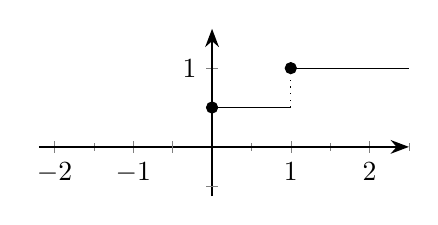
\begin{tikzpicture}[]
	\begin{axis}[
	x = 1cm,
	y = 1cm,
	axis lines=middle,
	axis line style={-Stealth,thick},
	xmin=-2.2,xmax=2.5,ymin=-0.625,ymax=1.5,
	xtick={-2,-1,0,1,2,3,4},
	ytick={0,1},
	extra x ticks={-0.5},
	extra y ticks={-0.5},
	extra x tick style={xticklabel=\empty},
	extra y tick style={yticklabel=\empty},
	xtick distance=1,
	ytick distance=1,
%	xlabel=$t$,
%	ylabel=$F(t)$,
	%title={Wonderful plot},
	minor tick num= 1,
	%grid=both,
	grid style={thin,densely dotted,black!20}]
	%\addplot [Latex-Latex,domain=-5:3,samples=2] {x*2/3} node[right]{$a$};
	\addplot [domain = 0:1] {0.5};
	\addplot [domain = 1:2.5] {1};	 
	\addplot [only marks] coordinates{(0,0.5)(1,1)};
	\addplot [dotted] coordinates{(1,0.5) (1,1)};
	\end{axis}
	\end{tikzpicture}
\end{center}	
Beide Modelle modellieren ein Experiment, bei dem zwei Elementarereignisse jeweils mit Wahrscheinlichkeit $\frac{1}{2}$ auftreten. Das zweite Modell ist nat\"urlich viel zu kompliziert, hat aber den Vorteil, dass wir reelle Zahlen bekommen. Der Vorteil ist, dass wir so zum Beispiel so etwas wie einen Mittelwert (hei\ss t sp\"ater Erwartungswert) definieren k\"onnen. Da wir den Ereignissen die Werte $0$ und $1$ geben, h\"attet ihr ohne viel nachzudenken sicherlich als umgangssprachlichen Erwartungswert $\frac 1 2$ vorgeschlagen.

Was unterscheidet Variante 1 von Variante 2? In der ersten Variante haben wir nur das zuf\"allige Experiment W\"urfeln modelliert in der zweiten Variante haben wir zwei Dinge auf einmal modelliert:
	\begin{itemize}
		\item Was passiert? (Welches zuf\"allige Ereigniss passiert beim W\"urfeln)
		\item Was wird ausgezahlt? (Was wird f\"ur Kopf bzw. Zahl ausgezahlt)
	\end{itemize}
Wenn wir bei Variante 1 auch \"uber Auszahlungen sprechen wollen, m\"ussen wir die m\"oglichen Elementarereignisse noch in Auszahlungen \"ubersetzen. Daf\"ur kommen messbare Abbildungen $X:\Omega \to \R$ ins Spiel.\smallskip	
	
 \textit{Ab jetzt:} Trenne in der Modellierung \enquote{Was passiert?} (also Ereignisse und Wahrscheinlichkeiten) von \enquote{Was wird beobachtet/ausgezahlt?}.
\end{disc}

\begin{deff}
\link{https://www.youtube.com/watch?v=7genugORczE&list=PLy5qRKPWp6SBwfc1kn-b66cWc84cOgvqZ&index=17&t=4105s}
	Ein \textbf{stochastisches Modell} besteht aus
	\begin{enumerate}[label=(\roman*)]
		\item einem Wahrscheinlichkeitsraum $(\Omega, \cA, \mathbb{P})$,
		\item einer $(\cA, \cB(\R))$-messbaren Abbildung $X\colon \Omega \to \R$.
	\end{enumerate}
	Dabei beschreibt (i) das zuf\"allige Experiment, (ii) beschreibt die \enquote{Beobachtung/Auszahlung}. $X$ wird auch \textbf{Zufallsvariable (ZV)} genannt. Eine konkrete Ausf\"uhrung $X(\omega)$ nennt man auch \textbf{Realisierung} der Zufallsvariablen. 
\end{deff}
Die \"Ubersetztung des Elementarereignisses $\omega$ in die Beobachtung $X(\omega)$ ist dabei deterministisch (nicht zuf\"allig), der Zufall steckt ausschlie\ss lich in dem Auftreten von $\omega$. Irgendjemand unbekanntes (die Physik, ein Computer, ein Gott, etc.) entscheidet \"uber die Wahl des zuf\"alligen $\omega$, das wird dann in die Zufallsvariable $X$ eingesetzt und wir beobachten den Wert $X(\omega)$. In dieser Vorlesung sprechen wir nicht weiter \"uber die \enquote{Ausf\"uhrung von Zufall}, wir modellieren Wahrscheinlichkeiten. F\"ur die Ausf\"uhrung von Zufall (wir sagen die Realisierung der Zufallsvariablen) verweisen wir auf Vorlesungen \"uber Monte Carlo Methoden oder Philosophie.
\begin{deff}\label{df}
\link{https://www.youtube.com/watch?v=7genugORczE&list=PLy5qRKPWp6SBwfc1kn-b66cWc84cOgvqZ&index=17&t=4813s}
Sei $X$ eine Zufallsvariable auf einem Wahrscheinlichkeitsraum $(\Omega, \mathcal A, \mathbb P)$.
	\begin{enumerate}[label=(\roman*)]
		\item Die \textbf{Verteilung der Zufallsvariablen $X$} ist definiert als
		\begin{gather*}
			\mathbb{P}_X (B) := \mathbb{P} (X \in B) \overset{\text{Notation}}{=} \mathbb{P}(\{ \omega \in \Omega \colon X(\omega) \in B \}) =\mathbb{P}(X^{-1}(B)), \quad B \in \cB(\R).
		\end{gather*}
		Unabh\"angig von dem zugrundeliegenden Wahrscheinlichkeitsraums ist $ \mathbb{P}_X $ also ein Maß auf $ \cB(\R) $ und zwar der push-forward von $\mathbb P$ unter $X$.
		\item Die \textbf{Verteilungsfunktion der Zufallsvariablen $X$} ist definiert als
		\[ F_X(t) := \mathbb{P}_X((-\infty,t]) \overset{\text{Def.}}{=} \mathbb{P}(X \leq t), \quad t \in \R. \]
		Wir schreiben $X \sim F_X$ und $X \sim \mathbb{P}_X$ und sagen \enquote{$X$ ist verteilt gemäß $F_X$ bzw. $X$ ist verteilt gem\"a\ss{} $\mathbb P_X$}.
	\end{enumerate}
	 Weil so viele Indizes nat\"urlich nerven, werden wir immer $X\sim F$ schreiben, wenn wir meinen, dass $X$ gem\"a\ss{} $F$ verteilt ist.  Wir sagen dann auch kurz \enquote{$X$ hat Verteilungsfunktion $F$}.
	 Beachte: Aufgrund der Definition ist nat\"urlich $\mathbb P_X=\mathbb P_{F_X}$, das werden wir immer mal wieder nutzen.
\end{deff}

Wir haben uns schon in der Ma\ss theorie langsam an den Begriff $\mu(\{f\leq t\})$ als Abk\"urzung f\"ur $\mu(\{\omega: f(\omega)\leq t\})$ gew\"ohnen m\"ussen. In der Stochastik gehen wir noch einen Schritt weiter und lassen die Klammern auch noch weg. Wir schreiben daher immer abk\"urzend
\begin{align*}
	\mathbb P(X< t),\quad \mathbb P(X\in (a,b]),\quad \mathbb P(X=a)
\end{align*}
und so weiter. Das liest sich als \glqq Wahrscheinlichkeit, dass $X$ kleiner als $t$ ist\grqq{} auch ziemlich nat\"urlich.



\begin{deff}
\link{https://www.youtube.com/watch?v=7genugORczE&list=PLy5qRKPWp6SBwfc1kn-b66cWc84cOgvqZ&index=17&t=5401s}
	Zufallsvariablen $X$ und $Y$, m\"oglicherweise auf verschiedenen Wahrschein-lichkeitsr\"aumen, heißen \textbf{identisch verteilt}, falls $F_X = F_Y$ bzw. $\mathbb P_X=\mathbb P_Y$. Man schreibt dann $X\sim Y$. Haben zwei Zufallsvariablen die gleiche Verteilungsfunktion, so sehen wir sie als gleichwertig an.
\end{deff}

	Zurück zum Münzwurf mit Auszahlung $1$ f\"ur Zahl und $0$ f\"ur Kopf. Wir schreiben dazu wieder zwei stochastische Modelle hin. Zum einen sei $\Omega = \{ \text{Kopf}, \text{ Zahl} \}$, $\cA = \cP(\Omega)$ und 
	\begin{align*}
		 \mathbb{P}(\{ \text{Kopf} \}) &= \mathbb{P}(\{ \text{Zahl} \}) = \frac{1}{2},\quad \mathbb{P}(\Omega) = 1, \quad \mathbb{P}(\emptyset) = 0,
	\end{align*}
	mit Zufallsvariable (Auszahlungsfunktion) definiert als
	\begin{align*}
		X(\text{Kopf})=0,\quad X(\text{Zahl})=1.
	\end{align*}
	Zum anderen sei $\Omega=\R$, $\cA = \cB(\R)$ und $\mathbb P=\mathbb{P}_F$ mit der Verteilungsfunktion
\begin{center}		
	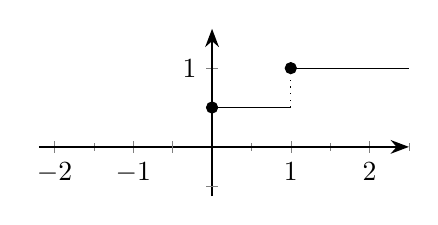
\begin{tikzpicture}[]
	\begin{axis}[
	x = 1cm,
	y = 1cm,
	axis lines=middle,
	axis line style={-Stealth,thick},
	xmin=-2.2,xmax=2.5,ymin=-0.625,ymax=1.5,
	xtick={-2,-1,0,1,2,3,4},
	ytick={0,1},
	extra x ticks={-0.5},
	extra y ticks={-0.5},
	extra x tick style={xticklabel=\empty},
	extra y tick style={yticklabel=\empty},
	xtick distance=1,
	ytick distance=1,
%	xlabel=$t$,
%	ylabel=$F(t)$,
	%title={Wonderful plot},
	minor tick num= 1,
	%grid=both,
	grid style={thin,densely dotted,black!20}]
	%\addplot [Latex-Latex,domain=-5:3,samples=2] {x*2/3} node[right]{$a$};
	\addplot [domain = 0:1] {0.5};
	\addplot [domain = 1:2.5] {1};	 
	\addplot [only marks] coordinates{(0,0.5)(1,1)};
	\addplot [dotted] coordinates{(1,0.5) (1,1)};
	\end{axis}
	\end{tikzpicture}
\end{center}		
	 Da wir diesmal die Auszahlung schon direkt im Modell modelliert haben, zahlen wir genau den Betrag aus, der zuf\"allig gezogen wird. Das machen wir mit der Zufallsvariablen $Y(\omega)=\omega$. Berechnen wir nun die Verteilungen der Zufallsvariablen $X$ und $Y$:
	\begin{align*}
		\mathbb P_X(B)&\overset{\text{Def.}}{=}\mathbb P(X\in B)=\begin{cases}
			\frac 1 2 &: 0\in B, 1\notin B\text{ oder } 1 \in B, 0\notin B\\
			1&: 0,1\in B\\
			0&: 0\notin B, 1\notin B
		\end{cases}\\
		&=\frac{1}{2} \delta_0(B)+\frac{1}{2}\delta_1(B)
	\end{align*}
	sowie
	\begin{align*}
		\mathbb P_Y(B)\overset{\text{Def.}}{=}\mathbb P(Y\in B)=\mathbb P(\{\omega \in \R: Y(\omega)\in B\})=\mathbb P(\{\omega \in \R: \omega \in B\})=\mathbb P(B)\overset{\text{Def.}}{=} \mathbb P_F(B).
	\end{align*}
	Weil $\mathbb P_F=\frac 1 2 \delta_0+\frac 1 2 \delta_1$, gilt also $\mathbb P_X=\mathbb P_Y$ bzw. $F_X=F_Y$. Damit sind $X$ und $Y$ identische verteilte Zufallsvariablen und wir sehen die beiden stochastischen Modelle als gleichwertige Modelle f\"ur den M\"unzwurf an.	
\marginpar{\textcolor{red}{Vorlesung 17}}


\begin{deff}
\link{https://www.youtube.com/watch?v=rm2_f1MRGoc&list=PLy5qRKPWp6SBwfc1kn-b66cWc84cOgvqZ&index=18&t=142s}
	\begin{enumerate}[label=(\roman*)]
		\item Eine Zufallsvariable $X$ heißt \textbf{absolutstetig} mit Dichte $f$, falls die Verteilungsfunktion $F_X$ von $X$ die Dichte $f$ hat, es gilt also
		\[ \mathbb{P}(X \in (a,b] ) =\mathbb P_X((a,b])= F_X(b) - F_X(a) = \int_{a}^{b} f(x) \dint x, \quad a<b. \]
		\item Eine Zufallsvariable $X$ heißt \textbf{diskret}, falls $F_X$ eine diskrete Verteilungsfunktion ist (oder $\mathbb P_X$ ein diskretes Ma\ss{} ist). In anderen Worten: $X$ nimmt nur abz\"ahlbar viele Werte $a_1,...,a_N$ mit Wahrscheinlichkeiten $p_1,...,p_N$ an:
			\begin{align*}
		 \mathbb{P}( X = a_k )=\mathbb P_X(\{a_k\})= p_k,\quad k=1,...,N.
		\end{align*}
	\end{enumerate}
\end{deff}
Ihr merkt euch am besten folgende Rechenformeln:
\begin{align*}
	\mathbb P(X\in A)=\begin{cases}
		\int_A f(x)\dint x&: X\text{ absolut stetig}\\
		\sum_{a_k\in A} p_k&: X\text{ diskret}
	\end{cases},
\end{align*}
man integriert oder summiert \"uber die Werte, die $X$ annehmen soll. Dumm ist nur, wenn wir nicht wissen, dass $X$ absolutstetig oder diskret ist. Dann ist eine Zufallsvariable halt irgendeine reellwertige messbare Abbildung auf irgendeinem Wahrscheinlichkeitsraum mit irgendeiner Verteilungsfunktion $F$.

\begin{beispiel}\label{link}
\link{https://www.youtube.com/watch?v=rm2_f1MRGoc&list=PLy5qRKPWp6SBwfc1kn-b66cWc84cOgvqZ&index=18&t=1197s}
	Wir kennen die meisten wichtigen Beispiele schon, manche kommen noch dazu:
	\begin{center}
	\begin{tabular}{l|l}
		Diskrete Zufallsvariablen& Absolutstetige Zufallsvariablen\\ %[0.05cm] 
		\hline
		$X \sim \operatorname{Poi}(\lambda)$& $X \sim \cN(\mu, \sigma^2)$\\
		$X \sim \operatorname{Bin}(n,p)$& $X \sim \operatorname{Cauchy}(s,t)$\\ 
		$X \sim \operatorname{Ber}(p)$& $X \sim \operatorname{Exp}(\lambda)$\\
		$X \sim \operatorname{Geo}(\lambda)$& $X \sim \cU([a,b])$\\
		$X \sim$ Gleichverteilt auf endlichem $\Omega$ & $X\sim\Gamma(\alpha,\beta)$\\
		&$X\sim \text{Pareto}(k,a)$
	\end{tabular}
	\end{center}
	Im Appendix gibt es eine \"Ubersicht \"uber die wichtigsten Verteilungen.
\end{beispiel}
Um die Begriffe auszuprobieren, schauen wir uns eine kleine Rechnung an. Wir behaupten, dass $Y\sim \operatorname{Exp}(1)$, wenn $Y=-\ln(U)$ mit $U\sim \mathcal U([0,1])$. Probieren wir die Begriffe aus und berechnen definitionsgem\"a\ss{} die Verteilungsfunktion von $Y$ durch Aufl\"osen:
\begin{align*}
	F_Y(t)=\mathbb P(Y\leq t) \overset{\text{Def.}}{=} \mathbb P(-\ln(U)\leq t)=\mathbb P(U\geq \exp(-t))=1-\mathbb P(U\leq \exp(-t)).
\end{align*}
Wenn wir jetzt die Verteilungsfunktion  von $\mathcal U([0,1])$ einsetzen, bekommen wir $F_Y(t)= (1-e^{-t})\mathbf 1_{[0,\infty)}(t)$ und das ist die Verteilungsfunktion der Exponentialverteilung.\smallskip 

 Wir waren ein klein wenig ungenau weil $Y$ den Wert $+\infty$ annehmen kann, eine Zufallsvariable per Definition aber nur reelle Werte annimmt. Das kann man einfach reparieren, indem man zum Beispiel $\log(0)=0$ umdefiniert. Alternativ nimmt man $U\sim \mathcal U((0,1))$ statt $U\sim \mathcal U([0,1])$, das diskutieren wir ausf\"uhrlich in Abschnitt \ref{sectrafo}.\smallskip


Es ist jetzt hoffentlich klar, was ein stochastisches Modell sein soll. Aber gibt es f\"ur jede Verteilungsfunktion \"uberhaupt solch Modell? Ja! Die in folgendem Beweis auftauchende Konstruk-tion hei\ss t \glqq kanonische Konstruktion\grqq{} und wird in der Stochastik in diversen Kontexten immer wieder benutzt.
\begin{satz}\label{existenz}
\link{https://www.youtube.com/watch?v=rm2_f1MRGoc&list=PLy5qRKPWp6SBwfc1kn-b66cWc84cOgvqZ&index=18&t=2131s} \textbf{[Existenz stochastischer Modelle]}
	Für jede Verteilungsfunktion $F$ existiert eine Zufallsvariable $X$ mit $X\sim F$. Genauer: Es existiert ein stochastisches Modell, \mbox{d. h.} ein Wahrscheinlichkeitsraum $(\Omega, \cA, \mathbb{P})$ und eine Zufallsvariable $X$ auf $(\Omega, \mathcal A, \mathbb P)$, mit $X \sim F$.
\end{satz}

\begin{proof}
	Als Wahrscheinlichkeitsraum definieren wir $\Omega=\R$, $\cA = \cB(\R)$, $\mathbb{P} = \mathbb{P}_F$ und darauf die Zufallsvariable $X(\omega) = \omega$. Beachte: $X(\omega)=\omega$ ist eine stetige Abbildung von $\R$ nach $\R$ und damit auch Borel-messbar. Berechnen wir die Verteilungsfunktion dieser konkreten Zufallsvariablen auf dem konkreten Wahrscheinlichkeitsraum:
		\begin{align*}
		F_X(t)=\mathbb P(X\leq t)=\mathbb P_F(\{\omega: X(\omega)\leq t\})=\mathbb P_F(\{\omega: \omega\leq t\})=\mathbb P_F((-\infty,t])=F(t),\quad t\in\R.
	\end{align*}
%	
%	\[ \mathbb{P}_X(B) = \mathbb{P}(X \in B) = \mathbb{P}_F(X \in B) = \mathbb{P}_F(\{ \omega \colon X(\omega) \in B \}) \overset{\text{Def. }X}{=} \mathbb{P}_F(B). \] 
	Also gilt $X\sim F$, das war es schon! Zu beachten ist, dass die Konstruktion weit von trivial ist. Die Existenz von $\mathbb P_F$ ben\"otigt den Satz von Carath\'eodory und damit die komplette Ma\ss theorie. 
\end{proof}

\begin{bem}
\link{https://www.youtube.com/watch?v=rm2_f1MRGoc&list=PLy5qRKPWp6SBwfc1kn-b66cWc84cOgvqZ&index=18&t=2625s}
	Wenn wir uns nur f\"ur diskrete Zufallsvariablen interessieren w\"urden, k\"amen wir komplett \textit{ohne} Maßtheorie aus! Hier ist eine viel einfachere Konstruktion, die f\"ur alle diskrete Zufallsvariablen funktioniert. Sei dazu $F$ eine diskrete Verteilungsfunktion, die an $N$-vielen Stellen $a_k$ um $p_k$ nach oben springt. Sei nun $\Omega=\{\omega_1,...,\omega_N\}$ eine beliebige Menge mit $N$ Elementen (z.B. $\Omega=\{\text{Kopf}, \text{Zahl}\}$ beim W\"urfeln). Auf $\Omega$ w\"ahlen wir als $\sigma$-Algebra $\mathcal A=\mathcal P(\Omega)$. Das Ma\ss{} definieren wir, indem wir es auf den Elementarereignissen als $\mathbb P(\{\omega_k\})=p_k$ definieren und mit der $\sigma$-Additivit\"at f\"ur beliebiges $A\in \mathcal A$ fortsetzen, d. h. $\mathbb P(A)=\sum_{\omega_k\in A} \mathbb P(\{\omega_k\})=\sum_{\omega_k\in A}p_k.$ An dieser Stelle nutzen wir die Abz\"ahlbarkeit. Als Zufallsvariable w\"ahlen wir die Abbildung $X(\omega_k):=a_k$. Weil auf dem Urbildraum die Potenzmenge gew\"ahlt wurde, ist nat\"urlich jede Abbildung nach $\R$ auch $(\mathcal A, \mathcal B(\R))$-messbar. Damit gilt $\mathbb{P}(X = a_k) = p_k$, also ist $X$ gem\"a\ss{} $F$ verteilt. Diese Konstruktion funktioniert nur f\"ur diskrete Verteilungsfunktionen so einfach (probiert es einfach mal f\"ur absolutstetige Verteilungsfunktionen aus, ihr werdet schnell den Fortsetzungssatz von Carath\'eodory brauchen). Im Allgemeinen kommen wir nicht umher, die Ma\ss theorie wie im Beweises von Satz \ref{existenz} zu nutzen weil man Ma\ss e auf \"uberabz\"ahlbaren Mengen nicht einfach auf den Elementarereignissen definieren kann.
\end{bem}
Hier sind zwei konkrete Beispiele: Wenn jemand von euch ein stochastisches Modell f\"ur eine $\mathcal N(0,1)$-verteilte Zufallsvariable verlangt, so entgegnet ihr
\begin{align*}
	\Omega=\R,\quad \mathcal A=\mathcal B(\R),\quad \mathbb P=\mathbb P_F,\quad X(\omega)=\omega,
\end{align*}
wobei $\mathbb P_F$ das eindeutige Ma\ss{} auf $\mathcal B(\R)$ mit Verteilungsfunktion $F\sim \mathcal N(0,1)$ aus Carath\'eodory ist. Will jemand das gleiche f\"ur eine $\text{Poi}(\lambda)$-verteilte Zufallsvariable haben, so entgegnet ihr entweder das gleiche, oder 
\begin{align*}
	\Omega=\mathbb N,\quad \mathcal A=\mathcal P(\mathbb N),\quad \mathbb P(\{k\})=e^{-\lambda} \frac{\lambda^k}{k!},\quad X(\omega)=\omega.
\end{align*}
Um ganz deutlich zu sein: Diskret ist einfach, weil die Potenzmenge von abz\"ahlbaren Mengen noch klein genug ist und Ma\ss e durch die abz\"ahlbare $\sigma$-Additivit\"at von Ma\ss en nur auf einpunktigen Mengen definiert werden m\"ussen! Weil all das f\"ur \"uberabz\"ahlbare Mengen wie $\R$ schief geht, haben wir Ma\ss theorie gemacht. Auf die Normalverteilung k\"onnen wir einfach nicht verzichten!
\begin{deff}
\link{https://www.youtube.com/watch?v=rm2_f1MRGoc&list=PLy5qRKPWp6SBwfc1kn-b66cWc84cOgvqZ&index=18&t=3524s}
	Ist $X$ eine Zufallsvariable auf $(\Omega, \cA, \mathbb{P})$, so heißen, falls die Integrale wohldefiniert sind,
	\begin{enumerate}[label=(\roman*)]
		\item \[ \mathbb{E}[X] := \int_{\Omega} X(\omega) \dint \mathbb{P}(\omega) \qquad \text{\textbf{Erwartungswert} von X}, \] 
		\item \[ \mathbb{E}[X^k] := \int_{\Omega} X^k(\omega) \dint \mathbb{P}(\omega) \qquad \text{\textbf{$k$-tes Moment} von X f\"ur }k\in\N, \]
		\item \[ \mathbb{V}[X] := \mathbb{E}[(X - \mathbb{E}[X])^2] \qquad \text{\textbf{Varianz} von X}, \]
		\item \[ \mathbb{E}[e^{\lambda X}] := \int_{\Omega} e^{\lambda X(\omega)} \dint \mathbb{P}(\omega) \qquad \text{\textbf{exponentielles Moment} von X f\"ur }\lambda\in\R. \]
	\end{enumerate}
	Allgemein betrachten wir f\"ur $g:\R\to\overline \R$ messbar die Erwartungswerte 
		\[ \mathbb{E}[g(X)] := \int_{\Omega} g(X(\omega)) \dint \mathbb{P}(\omega), \]
	falls das Integral wohldefiniert ist. Wir sagen die Erwartungswerte existieren, falls die Integrale existieren (also endlich sind).
\end{deff}
Wir erinnern daran, dass ein wohldefiniertes Integral auch die Werte $+\infty$ oder $-\infty$ annehmen darf. Meistens werden wir aber davon sprechen, dass die Integrale existieren, also endlich sind. Wegen der allgemeinen \"Aquivalenzen 
\begin{align*}
	\int f \dint \mu \text{ existiert } \quad\overset{\text{Def.}}&{\Leftrightarrow}\quad \int f^+ \dint \mu < \infty, \: \int f^- \dint \mu < \infty
	\quad{\Leftrightarrow}\quad \int |f| \dint \mu < \infty,
\end{align*}
schreiben wir meistens bequemer \enquote{$\mathbb{E}[|g(X)|] < \infty$} anstelle von \enquote{$\mathbb{E}[g(X)]$ existiert}. Bei Erwartungs-werten sagen wir also \enquote{der Erwartungswert von $X$ existiert}, wenn der Erwartungswert wohldefiniert und endlich ist. Das wird oft in der Literatur genauso gehandhabt, manchmal aber auch anders. Manche sagen, der Erwartungswert existiert, wenn $\E[X]$ wohldefiniert ist (aber vielleicht unendlich) ist.

\begin{bem1}
	Die Notation $\mathbb{E}[g(X)]$ ist etwas unglücklich weil das Integral nicht nur von $g$ und $X$ abh\"angt, sondern auch von $\mathbb P$. Daher sollte man eher  $\mathbb{E}_{\mathbb{P}}[g(X)]$ schreiben, man l\"asst aber \"ublicherweise das $\mathbb{P}$ aus Faulheit weg.
\end{bem1}

\begin{lemma}\label{ewTrafo}
\link{https://www.youtube.com/watch?v=rm2_f1MRGoc&list=PLy5qRKPWp6SBwfc1kn-b66cWc84cOgvqZ&index=18&t=4108s}
	Ist die Zufallsvariable $X$ gem\"a\ss{} $F$ verteilt, d. h. $X\sim F$, so gilt unabhängig von dem Wahrscheinlichkeitsraum $(\Omega, \cA, \mathbb{P})$ auf dem $X$ definiert ist,
	\[ \mathbb{E}[g(X)] = \int_{\R} g(x) \dint \mathbb{P}_F(x) \]
	für messbare numerische Abbildungen $g \colon \R \to \overline{\R}$. Wie immer gilt die Gleichheit, wenn eine Seite (und damit die die andere Seite) wohldefiniert ist.
\end{lemma}

\begin{proof}
	Mit dem Transformationssatz \ref{trafo} (bzw. Korollar (\ref{korTrafo}) gilt in einem Schaubild 
\begin{center}		
	\begin{tikzcd}
		{}&{}&{}\\
		(\Omega, \mathcal A, \mathbb P) \arrow[r, "{X}"] \arrow[rd, "{g \circ X}"']
		& (\R, \mathcal B(\mathbb{R}),\mathbb P_X) \arrow[d, "{g}"] \arrow[ur, phantom, "", near start] \\
		& (\overline{\R},\mathcal B(\overline{\R}))\\
	\end{tikzcd}
\end{center}
wobei $\mathbb P_X$ der push-forward von $X$ ist. Weil definitionsgem\"a\ss{} $\mathbb P_X=\mathbb P_F$ ist, gibt das sauber ausgeschrieben
\begin{align*}
	\E[g(X)] &\overset{\text{Def.}}{=} \int_{\Omega} g(X(\omega)) \dint \mathbb{P}(\omega)
	 \overset{\text{\ref{trafo}}}{=} \int_{\R} g(x) \dint \mathbb{P}_X(x)
	 \overset{\mathbb P_X=\mathbb P_F}{=} \int_{\R} g(x) \dint \mathbb{P}_F(x).
\end{align*}
\end{proof}
Die Konsequenz ist nat\"urlich, dass f\"ur beliebiges $g$, $\E[g(X)]$ gar nicht von dem kompletten Modell $(\Omega, \mathcal A, \mathbb P,X)$ abh\"angt, $\E[g(X)]$ h\"angt einfach nur von der Verteilung von $X$ ab. Das ist der Grund, warum man sich \"ublicherweise nur f\"ur die Verteilungsfunktion von $X$, jedoch nicht f\"ur $(\Omega, \mathcal A, \mathbb P)$ interessiert. Fassen wir die Beobachtung zusammen:
\begin{bem1}
	Sind $X, Y$ identisch verteilte Zufallsvariablen, die auf irgendwelchen Wahrscheinlich-keitsräumen definiert sind, so gilt
		\[ \mathbb{E}[g(X)] = \mathbb{E}[g(Y)] \] für alle $g \colon \R \to \overline{\R}$ messbar.
\end{bem1}
Jetzt wissen wir auch schon, wie wir $\E[g(X)]$ berechnen k\"onnen, das haben wir n\"amlich schon gemacht. Vieles was jetzt kommt sind Wiederholungen, indem wir S\"atze f\"ur allgemeine Integrale nochmal f\"ur Erwartungswerte hinschreiben.
\begin{satz}\label{regeln}
\link{https://www.youtube.com/watch?v=rm2_f1MRGoc&list=PLy5qRKPWp6SBwfc1kn-b66cWc84cOgvqZ&index=18&t=4583s} \textbf{[Berechnungsregeln]}
	Sei $X$ eine Zufallsvariable auf einem Wahrscheinlichkeitsraum $(\Omega, \mathcal A, \mathbb P)$ und $g:\R\to \overline{\R}$ messbar, so gelten:
	\begin{enumerate}[label=(\roman*)]
		\item\label{(i)} Ist $X$ absolutstetig mit Dichte $f$, so gilt \[ \mathbb{E}[g(X)] = \int_{\R} g(x) f(x) \dint x. \]
		\item\label{ii} Ist $X$ diskret und nimmt die Werte $a_1, ..., a_N\in\R$ mit Wahrscheinlichkeiten $p_1, ..., p_N$ an, so gilt
		 \[ \mathbb{E}[g(X)] = \sum\limits_{k=1}^{N} p_k\, g(a_k)=  \sum\limits_{k=1}^{N}  \mathbb{P}(X=a_k)g(a_k). \]
	\end{enumerate}
	 Dabei ist wieder eine Seite genau dann wohldefiniert, wenn es die andere Seite ist.
\end{satz}
\begin{proof}
	Dazu kombinieren wir nur die Formel aus Satz	\ref{ewTrafo} mit den Formeln aus Satz \ref{IntDichten} und Satz \ref{IntDiskr}.
\end{proof}

\begin{beispiel}\link{https://www.youtube.com/watch?v=rm2_f1MRGoc&list=PLy5qRKPWp6SBwfc1kn-b66cWc84cOgvqZ&index=18&t=4924s} \abs

	\begin{itemize}
		\item F\"ur $X \sim \cN(\mu, \sigma^2)$ gilt $ \mathbb{E}[X] = \int_{\R} x \frac{1}{\sqrt{2\pi\sigma^2}} e^{-\frac{(x-\mu)^2}{2 \sigma^2}}\dint x = \mu$.
		\item F\"ur $X \sim \operatorname{Ber}(p)$ gilt $ \mathbb{E}[X] = 1 \cdot \mathbb{P}(X = 1) + 0 \cdot \mathbb{P}(X = 0) = p$.
		\item F\"ur $X \sim \operatorname{Poi}(\lambda)$ gilt $ \mathbb{E}[X] = \sum_{k = 0}^{\infty} k \cdot \mathbb{P}(X = k) = \sum_{k = 0}^{\infty} k e^{-\lambda} \frac{\lambda^k}{k!} = \lambda$.
	\end{itemize}
	Wir sehen also: Ein gro\ss er Teil der Stochastik besteht aus dem Berechnen von Integralen und Summen bzw. Reihen.
\end{beispiel}
\marginpar{\textcolor{red}{Vorlesung 18}}

\begin{beispiel}
\link{https://www.youtube.com/watch?v=JbjvBFpbsho&list=PLy5qRKPWp6SBwfc1kn-b66cWc84cOgvqZ&index=19&t=113s}
	Eine Webseite wird im Mittel pro Stunde zweimal geklickt. Wie groß ist die Wahrscheinlichkeit, dass die Webseite in einer Stunde mindestens fünfmal geklickt wird?\smallskip
	
	Um das Beispiel stochastisch zu behandeln, m\"ussen wir zun\"achst ein Modell annehmen. Welche uns bekannte Zufallsvariable k\"onnte die Anzahl der Klicks pro Stunde modellieren? Da die Ergebnisse der Zufallszahlen nat\"urliche Zahlen sind, muss die Verteilung diskret sein. Nun ist die Anzahl nicht beschr\"ankt, es sollte also eine Zufallsvariable sein, die alle Werte in $\N$ annehmen kann. Dazu kennen wir bisher nur die geometrische- oder die Poissonverteilung. An der jetzigen Stelle k\"onnen wir ohne weitere Annahmen keine von beiden ausschlie\ss en. Nehmen wir einfach mal an, dass $X\sim \operatorname{Poi}(\lambda)$ ein gutes Modell ist. Aber was ist $\lambda$? Weil wir wissen, dass $\E[X]=\lambda$ ist, schlie\ss en wir $\lambda=2$ aus der Vorinformation (Das Gesetz der gro\ss en Zahlen wird uns in Satz \ref{sGGZ} des letzten Kapitel die Rechtfertigung geben, warum wir aus dem Mittel auf den Erwartungswert schlie\ss en.) Um nun die Aufgabe zu l\"osen, m\"ussen wir f\"ur eine $\operatorname{Poi}(2)$-verteilte Zufallsvariable $\mathbb P(X\geq 5)$ berechnen. Das geht ganz einfach:
	\begin{align*}
	\mathbb{P}(X \geq 5) &= 1 - \mathbb{P}(X \leq 4)\\
	& = 1 - \sum\limits_{k=0}^{4} \mathbb{P}(X = k)\\ 
	&= 1 - e^{-2} \left(\frac{1}{1} + \frac{2}{1} + \frac{4}{2} + \frac{8}{6} + \frac{16}{24}\right) \approx 0,053.
	\end{align*} 
	Hierbei haben wir genutzt, dass f\"ur eine diskrete Zufallsvariable immer $$\mathbb P(X\in A)=\sum_{a_k\in A} \mathbb P(X=a_k)$$ gilt. Das folgt nat\"urlich aus der $\sigma$-Additivit\"at von Ma\ss en weil $A\mapsto \mathbb P(X\in A)$ ein Ma\ss{} ist (die Verteilung von $X$).
	\end{beispiel}


\begin{prop}\label{rechenregeln}
\link{https://www.youtube.com/watch?v=JbjvBFpbsho&list=PLy5qRKPWp6SBwfc1kn-b66cWc84cOgvqZ&index=19&t=1157s} \textbf{[Rechenregeln f\"ur den Erwartungswert]}
	Seien $X,Y$ Zufallsvariablen auf $(\Omega, \cA, \mathbb{P})$ mit $\mathbb{E}[|X|],\mathbb{E}[|Y|] < \infty$ und $\alpha,\beta\in\R$, so gelten:
	\begin{enumerate}[label=(\roman*)]
		\item $\mathbb{E}[\alpha X + \beta Y] = \alpha \mathbb{E}[X] + \beta \mathbb{E}[Y]$
		\item $X \geq 0$ $\mathbb P$-f.s. $\Rightarrow \mathbb{E}[X] \geq 0$ und  $X \geq Y$ $\mathbb P$-f.s. $\Rightarrow \mathbb{E}[X] \geq \mathbb{E}[Y]$
		\item Ist $X = \alpha$  $\mathbb{P}$-f.s., so ist $\mathbb{E}[X] = \alpha$.
		\item $\mathbb{P}(X \in A) = \mathbb{E}[\mathbf{1}_A(X)]$, insbesondere gilt $F_X(t)=\E[\mathbf 1_{(-\infty,t]}(X)]$, $t\in\R$.
	\end{enumerate}
\end{prop}

\begin{proof}
	Wir m\"ussen nur beachten, dass Erwartungswerte per Definition Integrale sind. Dann k\"onnen wir die Rechenregeln f\"ur Integrale direkt anwerden. Zu beachten ist, dass wegen Satz \ref{S7} \"Anderungen auf Nullmengen Integrale nicht \"andern.
	\begin{enumerate}[label=(\roman*)]
	\item Linearität von Integralen
	\item Monotonie von Integralen (die Nullmengen spielen keine Rolle)
	\item Nach Annahme gilt $X = \alpha \mathbf{1}_{\Omega}$ $\mathbb{P}$-f.s. Wegen Satz \ref{S7} k\"onnen wir sofort die Definition des Integrals einsetzen:
	\[ \mathbb{E}[X] = \int_{\Omega} X(\omega) \dint \mathbb{P}(\omega) = \int_{\Omega} \underbrace{\alpha \mathbf{1}_{\Omega}}_{\text{einfach}} \dint \mathbb{P} \overset{\text{Def.}}{=} \alpha \mathbb{P}(\Omega) = \alpha  \]
	\item Hier m\"ussen wir nur die Definitionen im Kopf klar bekommen:
	\begin{gather*}
		\mathbb{E}[\mathbf{1}_A(X)] = \int_{\Omega} \mathbf{1}_A(X(\omega)) \dint \mathbb{P}(\omega) \overset{\text{Trafo}}{=} \int_{\R} \underbrace{\mathbf{1}_A(x)}_{\text{einfach}} \dint \mathbb{P}_X(x) = \mathbb{P}_X(A) \overset{\text{Def.}}{=} \mathbb{P}(X \in A)
	\end{gather*}
\end{enumerate}
\end{proof}
Nat\"urlich ist eine Zufallsvariable, die fast sicher den selben Wert annimmt, gar keine interessante Zufallsvariable! Das modellierte Zufallsexperiment ist gar nicht zuf\"allig, es passiert immer das gleiche! Beispiel: Jeden Tag um 7 Uhr wird die Zeit (Stunde) angeschaut. Es kommt immer $7$ dabei raus, die beschreibende Zufallsvariable erf\"ullt also $\mathbb P(X=7)=1$, also $X=7$ $\mathbb P$-fast sicher. Viel interessanter w\"are zum Beispiel, jeden Tag um 7 Uhr die Temperatur zu messen. Die entsprechende Zufallsvariable w\"are nicht fast sicher konstant.
\begin{korollar}\label{vari}
\link{https://www.youtube.com/watch?v=JbjvBFpbsho&list=PLy5qRKPWp6SBwfc1kn-b66cWc84cOgvqZ&index=19&t=2008s} \textbf{[Rechenregeln f\"ur die Varianz]}
	Sei $X$ eine Zufallsvariable mit $ \mathbb{E}[X^2] < \infty$ (wir sagen auch, $X$ ist quadratintegrierbar), so gelten:
	\begin{enumerate}[label=(\roman*)]
		\item Es gilt $ \mathbb{V}[X] < \infty$ und \[ \mathbb{V}[X] = \mathbb{E}[X^2] - \mathbb{E}[X]^2. \]
		\item	Es gilt $ \mathbb{V}[X]= 0$ genau dann, wenn $X$ fast sicher den gleichen Wert annimmt, dieser ist dann $\E[X]$.
		\item F\"ur $a\in \R$ gilt $\V[aX]=a^2 \V[X]$ und $\V[a+X]=\V[X]$.	
\end{enumerate}
\end{korollar}

\begin{proof}
	Übung. Beachte dazu: Ist $Y \geq 0$ $\mathbb{P}$-fast sicher und $ \mathbb{E}[Y] = 0$, so ist $ Y \equiv 0$ $\mathbb P$-fast sicher. Das gilt wegen Satz \ref{S7}, der Erwartungswert ist schlie\ss lich ein Integral!
\end{proof}
Die Varianz misst als Kenngr\"o\ss e die Variabilit\"at von Zufallsvariablen. Ist die Varianz null, so gibt es gar keine Variabilit\"at, ist die Varianz gro\ss, so nimmt $X$ auch Werte an, die weit von dem Erwartungswert entfernt sind. Das ist mathematisch nat\"urlich keine saubere Formulierung (daf\"ur gibt es schlie\ss lich die Varianz), gibt aber das richtige Gef\"uhl. Daher ist auch einleuchtend, dass sich die Variabilit\"at beim Verschieben um einen festen Wert sich nicht \"andert.



\begin{satz}
\link{https://www.youtube.com/watch?v=JbjvBFpbsho&list=PLy5qRKPWp6SBwfc1kn-b66cWc84cOgvqZ&index=19&t=2482s} \textbf{[Konvergenzsätze für Zufallsvariablen]}
	Seien $Y,X,X_1,X_2,...$ Zufallsvariablen auf $(\Omega, \cA, \mathbb{P})$ mit $\lim_{n\to\infty} X_n=X$ $\mathbb{P}$-fast sicher.
	\begin{enumerate}[label=(\roman*)]
		\item MCT: Gilt $0 \leq X_1\leq X_2\leq ...\leq X$ $\mathbb{P}$-fast sicher, so gilt 
		\[ \lim\limits_{n \to \infty} \mathbb{E}[X_n] = \mathbb{E}[X]. \]
				\item DCT: Gilt $|X_n| \leq Y$ $\mathbb{P}$-fast sicher für alle $n \in \N$ mit $\E[|Y|]<\infty$, so gilt
		\[ \lim\limits_{n \to \infty} \mathbb{E}[X_n] = \mathbb{E}[X]. \]
		\item Gilt $|X_n| \leq C$ $\mathbb{P}$-fast sicher für alle $n \in \N$ f\"ur ein $C>0$, so gilt
		\[ \lim\limits_{n \to \infty} \mathbb{E}[X_n] = \mathbb{E}[X]. \]
	\end{enumerate}
\end{satz}

\begin{proof}
	Wegen $\mathbb{E}[X_n] \overset{\text{Def.}}{=} \int_{\Omega} X_n \dint \mathbb{P}$ und $\mathbb{E}[X] \overset{\text{Def.}}{=} \int_{\Omega} X \dint \mathbb{P}$ ist das gerade Satz \ref{allgMonKonv}, Satz \ref{DCT} und Korollar \ref{K7}. 
\end{proof}

\begin{deff}
\link{https://www.youtube.com/watch?v=JbjvBFpbsho&list=PLy5qRKPWp6SBwfc1kn-b66cWc84cOgvqZ&index=19&t=2922s}
	F\"ur eine Zufallsvariable $X$ heißt $$\cM_X(t) := \mathbb{E}[e^{tX}], \quad t\in\R,$$ die \textbf{momenterzeugende Funktion}. $\cM_X$ ist nur für die $t$ definiert, für die $\mathbb{E}[e^{tX}] < \infty$ gilt.
\end{deff}

Die momenterzeugenden Funktionen sind auf ihrem Definitionsbereich ganz normale Funktionen von $\R$ nach $\R$. Wir k\"onnen also \"uber Ableitungen sprechen, Monotonie, und so weiter. In vielen Beispielen ist $M_X$ eine ganz harmlose Funktion, manchmal ist $\cM_X$ aber auch gar nicht definiert.
\begin{beispiel}\link{https://www.youtube.com/watch?v=JbjvBFpbsho&list=PLy5qRKPWp6SBwfc1kn-b66cWc84cOgvqZ&index=19&t=3284s} \abs

\begin{itemize}
	\item Sei $ X \sim \operatorname{Cauchy}(s,t)$, so ist $\cM_X$ nirgends definiert!
	\item Sei $X \sim \cN(\mu, \sigma^2)$, so ist $\cM_X(t) = \exp\big(\mu t + \frac{\sigma^2 t^2}{2}\big)$ f\"ur $t\in\R$, siehe \"Ubungsaufgabe.
	\item Sei $X\sim \operatorname{Poi}(\lambda)$, so ist $$\cM_X(t) = \mathbb{E}[e^{tX}] = \sum\limits_{k=0}^{\infty} e^{tX} \mathbb{P}(X = k) = \sum\limits_{k=0}^{\infty} e^{tk} e^{-\lambda} \frac{\lambda^k}{k!} = e^{\lambda(e^t - 1)}$$ f\"ur alle $t\in\R$.
	\end{itemize}
Noch viel mehr explizite Beispiele sind im Appendix gesammelt.
\end{beispiel}

Das ganze ist ein so n\"utzliches Konzept, weil wir viele Beispiele explizit ausrechnen k\"onnen und mit dem n\"achsten Satz gleich noch alle Momente durch Ableiten ausrechnen k\"onnen:

\begin{satz}\label{erzeugende}
\link{https://www.youtube.com/watch?v=JbjvBFpbsho&list=PLy5qRKPWp6SBwfc1kn-b66cWc84cOgvqZ&index=19&t=3545s}
	Sei $X$ eine Zufallsvariable, f\"ur die f\"ur irgendein $\varepsilon>0$ die Momenterzeugende Funktion $\cM_X$ auf $(-\varepsilon, \varepsilon)$ definiert ist. Dann ist $\cM_X$ an der Stelle $0$ unendlich oft differenzierbar und es gilt f\"ur alle $n\in\mathbb N$ $$\mathbb{E}[X^n] = \cM_X^{(n)}(0),$$ wobei $\cM_X^{(n)}(0)$ die $n$-te Ableitung an der Stelle $0$ ist.
\end{satz}





\begin{proof}\abs
	\begin{enumerate}[label=(\alph*)]
		\item Wir zeigen zun\"achst, dass $\cM_X$ in $(-\varepsilon,\varepsilon)$ eine Potenzreihe ist. Nach Analysis 1 gilt punktweise (also f\"ur jedes $\omega\in \Omega$)
		\[ e^{tX(\omega)} = \sum\limits_{k=0}^{\infty} \frac{(tX(\omega))^k}{k!} = \lim\limits_{m \to \infty} \sum\limits_{k=0}^{m} \frac{(tX(\omega))^k}{k!} =: \lim\limits_{m \to \infty} S_m (\omega). \]
		Die Zufallsvariable $e^{tX}$ kann also als punktweiser Grenzwert der Folge $(S_m)_{m\in\N}$ von Zufallsvariablen geschrieben werden. Um gleich dominierte Konvergenz zu nutzen, brauchen wir eine integrierbare Majorante $S$ f\"ur die Folge $(S_m)$. Das ist gar nicht so schwer: \[ |S_m| \overset{\text{Def.}}{=} \Big|\sum\limits_{k=0}^{m} \frac{(tX)^k}{k!} \Big| \overset{\triangle}{\leq} 
		\sum\limits_{k=0}^{m} \Big| \frac{(tX)^k}{k!} \Big| \leq \sum\limits_{k=0}^{\infty} \Big| \frac{(tX)^k}{k!} \Big| =: S.
		\]
		Wegen $S=e^{|tX|} \leq e^{tX} + e^{-tX}$ ist $S$ eine integrierbare Majorante:
		\[ \mathbb{E}[|S|] = \mathbb{E}[e^{|tX|}] \overset{\text{Mon.}}{\underset{\text{Lin.}}{\leq}} \mathbb{E}[e^{tX}] + \mathbb{E}[e^{-tX}] \overset{\text{Def.}}{=} \cM_X(t) + \cM_X(-t) < \infty
		\]
		f\"ur $t\in (-\varepsilon,\varepsilon)$ nach Annahme. Jetzt kann also dominierte Konvergenz angewandt werden. Es gilt damit f\"ur $t\in (-\varepsilon,\varepsilon)$, dass
		\begin{align*}
		M_X(t)=\E[\lim_{m\to\infty} S_m] \overset{\text{DCT}}{=} \lim_{m\to\infty} \E[S_m]\overset {\text{Lin.}}{=} \lim_{m\to\infty} \sum_{k=0}^m\frac{t^k \E[X^k]}{k!}=\sum_{k=0}^\infty\frac{t^k \E[X^k]}{k!}.
		\end{align*}
		Damit ist $M_X$ in $(-\varepsilon,\varepsilon)$ eine Potenzreihe mit Koeffizienten $a_k=\frac{\E[X^k]}{k!}$ und Entwicklungspunkt $x_0=0$.
		\item	Aus Analysis 1 wisst ihr (so habt ihr die Taylor-Koeffizienten bestimmt!), dass $M_X$ in $(-\varepsilon, \varepsilon)$ unendlich oft differenzierbar ist und die Reihe gliedweise differenziert werden kann. $n$-faches Ableiten und den Entwicklungspunkt $x_0=0$, einsetzen gibt dann $M_X^{(n)}(0)=\E[X^n]$.
	\end{enumerate}
\end{proof}

\begin{beispiel} \link{https://www.youtube.com/watch?v=JbjvBFpbsho&list=PLy5qRKPWp6SBwfc1kn-b66cWc84cOgvqZ&index=19&t=4776s} \abs

	\begin{itemize}
		\item F\"ur die Normalverteilungen $X \sim \cN(\mu, \sigma^2)$ ergibt die explizite Formel der momenterzeugenden Funktion mit dem Satz
		\begin{align*}
		\mathbb{E}[X] &= \cM_X'(0) = \exp\Big(\mu\cdot0 + \frac{\sigma^2 t^2}{2}\Big)\cdot (\mu + \sigma^2 \cdot 0) = \mu, \\
		\mathbb{E}[X^2] &= \cM_X''(0) = \mu^2 + \sigma^2.
		\end{align*}
		Beides zusammen ergibt $\mathbb{V}[X] = \mathbb{E}[X^2] - \mathbb{E}[X]^2 = \mu^2 + \sigma^2 - \mu^2 = \sigma^2$. Die zwei Parameter der Normalverteilung sind also gerade Erwartungswert $\mu$ und Varianz $\sigma^2$.
		\item F\"ur $X \sim \operatorname{Poi}(\lambda)$ ergibt die explizite Formel der momenterzeugenden Funktion mit dem Satz
		\begin{align*}
		\mathbb{E}[X] = \cM_X'(0) = \lambda \quad \text{ und }\quad  \mathbb{E}[X^2] = \cM_X''(0) = \lambda^2 + \lambda.
		\end{align*}
		Beides zusammen ergibt $\mathbb{V}[X] = \mathbb{E}[X^2] - \mathbb{E}[X]^2 =\lambda$.
	\end{itemize}
\end{beispiel}


\begin{prop}\label{jensen}
\link{https://www.youtube.com/watch?v=JbjvBFpbsho&list=PLy5qRKPWp6SBwfc1kn-b66cWc84cOgvqZ&index=19&t=5002s} \textbf{[H\"older und Jensen’sche Ungleichung]}


\begin{itemize}
\item[(i)] F\"ur $p,q>1$ mit $\frac{1}{p}+\frac{1}{q}=1$ und Zufallsvariablen $X,Y$ auf $(\Omega, \mathcal A, \mathbb P)$ gilt
\begin{align*}
	\mathbb E[|XY|]\leq \big(\mathbb E[|X|^p]\big)^{1/p} \big(\mathbb E[|Y|^q]\big)^{1/q}.
\end{align*}
\item[(ii)]
	Ist $X$ eine Zufallsvariable mit $\mathbb{E}[|X|] < \infty$ und $\varphi \colon \R \to \R $ \textit{konvex} mit $\mathbb{E}[|\varphi(X)|] < \infty$, so gilt
	\[ \varphi(\mathbb{E}[X]) \leq \mathbb{E}[\varphi(X)]. \]
\end{itemize}
\end{prop}


\begin{proof}
(i) Weil Erwartungswerte Integrale sind, ist das nur ein Spezialfall von Satz \ref{hoelder}.\smallskip

(ii) Wir geben den Beweis nur f\"ur differenzierbares $\varphi$. Wegen der Konvexität gibt es f\"ur jedes feste $x_0 \in \R$ ein $b\in\R$ mit
	\begin{itemize}
		\item $ \varphi'(x_0) x + b \leq \varphi(x)$ f\"ur alle $x\in\R$,
		\item $ \varphi'(x_0) x_0 + b = \varphi(x_0)$.
	\end{itemize}
	Wir w\"ahlen $x_0 = \E[X]$. Mit der zweiten Eigenschaft schreiben wir $\varphi(\E[X])$ wie folgt um:
	\begin{align*}
	\varphi(\E[X]) = \varphi(x_0) = \varphi'(x_0) x_0 + b = \varphi'(x_0) \E[X] + b.
	\end{align*}
	Weil der Erwartungswert linear und monoton ist, sowie der Erwartungswert einer konstanten Zufallsvariable gerade die Konstante ist, k\"onnen wir die rechte Seite wie folgt behandeln:
	\begin{align*}	
	\varphi'(x_0) \E[X] + b= \E[\varphi'(x_0) X] + \E[b] = \E[\varphi'(x_0) X + b] \overset{\text{Mon.}}{\leq} \E[\varphi(x)].
	\end{align*}
	Zusammen folgt die Behauptung.
\end{proof}

\begin{beispiel1}
	Als Merkregel für das \enquote{$\leq$} in Proposition \ref{jensen} nimmt man $\varphi(x)=x^2$. Weil
	\[ 0 \leq \V(X) = \E[(X - \E[X])^2] \overset{\text{Üb.}}{=} \E[X^2] - \E[X]^2,
	\]
	muss $\E[X]^2\leq \E[X^2]$ gelten. Also muss in \ref{jensen} \enquote{$\leq$} und nicht \enquote{$\geq$} stehen.
\end{beispiel1}
\marginpar{\textcolor{red}{Vorlesung 19}}
Zum Abschluss nochmal die Markov- und Tschebyscheff-Ungleichungen, die wir f\"ur Integrale \"uber beliebige Ma\ss e schon angeschaut haben. Weil Erwartungswerte Integrale sind, geht das in diesem Spezialfall nat\"urlich genauso:
\begin{satz}\label{Markov}
\link{https://www.youtube.com/watch?v=T4qzzuYLcUc&list=PLy5qRKPWp6SBwfc1kn-b66cWc84cOgvqZ&index=20&t=415s} \textbf{[Markov- und Tschebyscheff-Ungleichung]}
	Sei $X$ eine Zufallsvariable, dann gelten für alle $a > 0$ folgende Ungleichungen:
	\begin{enumerate}[label=(\roman*)]
		\item F\"ur $h \colon \R \to (0, \infty)$ wachsend gilt
		 \[ \mathbb{P}(X\geq a) \leq \frac{\E[h(X)]}{h(a)} \quad\quad \text{(Markov-Ungleichung)} \]
		\item F\"ur $h \colon [0,\infty) \to (0, \infty)$ wachsend gilt		
		 \[ \mathbb{P}(|X|\geq a) \leq \frac{\E[h(|X|)]}{h(a)} \quad\quad \text{(Markov-Ungleichung)} \]
		\item \[ \mathbb{P}(|X - \E[X]| \geq  a) \leq \frac{\V[X]}{a^2} \quad\quad \text{(Tschebyscheff-Ungleichung)} \]
	\end{enumerate}
\end{satz}

\begin{proof}\abs
	\begin{enumerate}[label=(\roman*)]
		\item \label{itscheby} Definiere $A = [a, \infty)$, dann gilt weil $h$ wachsend ist
		\begin{align*}
		\E[h(X)] \overset{\text{Mon.}}&{\geq} \E[h(X) \cdot \mathbf{1}_A(X)] \\
		&\geq \E[h(a) \cdot \mathbf{1}_A(X)]\\
		 \overset{\text{Lin.}}&{=} h(a) \cdot \E[\mathbf{1}_A(X)]\\
		\overset{\ref{rechenregeln}, (iv)}&{=} h(a) \cdot \mathbb{P}(X\geq a).
		\end{align*}
		Durchteilen gibt die Absch\"atzung. Hier haben wir den kleinen Trick genutzt, dass $1\equiv \mathbf 1_{\Omega}\equiv \mathbf 1_A+\mathbf 1_{A^C}\geq \mathbf 1_A$ gilt. Der Trick wird jetzt immer wieder kommen!
		\item Genau wie (i).
		\item Benutze die Markov Ungleichung mit $h(x) = x^2$ und der \enquote{zentrierten} Zufallsvariablen $X - \E[X]$.
	\end{enumerate}
\end{proof}
Wie bei den Konzentrationsungleichungen f\"ur Ma\ss e, k\"onnen wir durch Bildung von Gegenwahr-scheinlichkeiten sofort Ungleichungen f\"ur $\mathbb{P}(X<a)$ oder $\mathbb P(|X|<a)$ bekommen. Hier ein konkretes Beispiel: Ist $ X \sim \cN(\mu, \sigma^2)$, so gilt $ \mathbb{P}(|X - \mu| \geq a) \leq \frac{\sigma^2}{a^2}$.


\section{Zufallsvektoren}\label{sec:ZV}
Nachdem Zufallsvariablen jetzt hoffentlich einigerma\ss en klar geworden sind, gehen wir jetzt weiter zu Zufallsvektoren. Das sind Zufallsvariablen, deren Werte nicht reell, sondern aus dem $\R^d$ sind. Weil wir den Namen Zufallsvariablen nur f\"ur den Fall $d=1$ definiert haben, sprechen wir nun von Zufallsvektoren. Das Kapitel ist in gro\ss en Teilen eine Wiederholung, wir gehen durch die gleichen Schritte, die Notationen werden nur einen Tick aufwendiger. Das Vorgehen ist genau wie f\"ur reelle (eindimensionale) Zufallsvariablen: 
\begin{itemize}
	\item Lege $\sigma$-Algebra auf $\R^d$ fest und zeige wichtige Eigenschaften f\"ur sp\"ater.
	\item Charakterisiere Maße auf $\R^d$ durch Verteilungsfunktionen.
	\item Definiere Zufallsvektoren als messbare Abbildungen und verbinde diese zu Ma\ss en und Verteilungsfunktionen. 
	\item Definiere Erwartungswerte und zeige Rechnenregeln f\"ur diskrete und absolutstetige Zufallsvektoren.
	\item Rechnen, rechnen, rechnen.
\end{itemize}

\subsection*{(A) Borel-$\sigma$-Algebra auf $\R^d$}

\begin{deff}
\link{https://www.youtube.com/watch?v=T4qzzuYLcUc&list=PLy5qRKPWp6SBwfc1kn-b66cWc84cOgvqZ&index=20&t=1977s}
	Wir w\"ahlen die Produkt-$\sigma$-Algebra auf dem $\R^d$, die aus $d$ Kopien der Borel-$\sigma$-Algebra besteht:
	\[ \cB(\R^d) := \underbrace{\cB(\R) \otimes ... \otimes \cB(\R)}_{d\text{-viele}} \overset{\text{Def.}}{=} \sigma(\{ B_1 \times ... \times B_d \colon B_i \in \cB(\R) \}) \]
\end{deff}
Wir hatten im ersten Kapitel schon erw\"ahnt, dass die Definition der Borel-$\sigma$-Algebra als kleinste $\sigma$-Algebra erzeugt durch offene Mengen auch im $\R^d$ funktioniert. Das ist in der Tat das selbe wie die gerade definierte Produkt-$\sigma$-Algebra $\mathcal B(\R^d)$. 
\begin{lemma}
\link{https://www.youtube.com/watch?v=T4qzzuYLcUc&list=PLy5qRKPWp6SBwfc1kn-b66cWc84cOgvqZ&index=20&t=2103s}
	Es gilt 
	\begin{align*}
		\cB(\R^d) &= \sigma(\{ O \subseteq \R^d\colon O \text{ offen} \})\\
		& = \sigma(\{ (-\infty,t_1] \times ... \times (-\infty,t_d] \colon t_i \in \R \})\\
		& = \sigma(\{ (a_1,b_1]\times ... \times (a_d,b_d] \colon a_i,b_i \in \R \})\\
		& = \sigma(\{ (a_1,b_1) \times ... \times (a_d,b_d) \colon a_i,b_i \in \R \})\\
		&=...,
	\end{align*}
	wobei ... bedeutet, dass ihr wie f\"ur $d=1$ alle vorstellbaren Kombinationen von Intervallen nutzen k\"onnt.	
\end{lemma}

\begin{proof}
	Übungsaufgabe.
\end{proof}
\begin{bem} \link{https://www.youtube.com/watch?v=T4qzzuYLcUc&list=PLy5qRKPWp6SBwfc1kn-b66cWc84cOgvqZ&index=20&t=2340s}
	Wie in Dimension $1$ gilt auch jetzt wieder, dass jede stetige Abbildung $f\colon \R^n \to \R^m$  $(\cB(\R^n), \cB(\R^m))$-messbar ist. Das gilt wieder weil wegen Proposition \ref{S2} Messbarkeit nur auf einem beliebigen Erzeuger getestet werden muss und f\"ur stetige Abbildungen Urbilder offener Mengen offen sind.
\end{bem}

\subsection*{(B) Maße auf $\mathcal B(\R^d)$ und multivariate Verteilungsfunktionen}
Wie f\"ur $d=1$ definieren wir f\"ur Ma\ss e auf $\mathcal B(\R^d)$ Verteilungsfunktionen, der Unterschied ist nur die Anzahl der Variablen, $d$ viele statt einer:
\begin{deff}
\link{https://www.youtube.com/watch?v=T4qzzuYLcUc&list=PLy5qRKPWp6SBwfc1kn-b66cWc84cOgvqZ&index=20&t=2573s}
	Ist $\mathbb{P}$ ein Wahrscheinlichkeitsmaß auf $ \cB(\R^d) $, so heißt $$F_{\mathbb{P}}(t_1,...,t_d) = \mathbb{P}((-\infty, t_1] \times \dots \times (-\infty, t_d]),\quad t_1,...,t_d\in\R,$$ \textbf{(multivariate) Verteilungsfunktion} von $\mathbb{P}$.
\end{deff}
F\"ur die Vorstellung nehmen wir immer den Fall $d=2$. Dann ist $F(t_1,t_2)$ gerade das Ma\ss{} des \enquote{unendlichen Rechtecks unten links} unter dem Punkt $(t_1,t_2)$, also das Ma\ss{} von $(\infty, t_1]\times (-\infty,t_2].$\smallskip

Wie f\"ur $d=1$ (nichtfallend, rechtsstetig, Grenzwerte $1$ und $0$ bei unendlich) k\"onnen wir aus den Eigenschaften des Ma\ss es Eigenschaften der Verteilungsfunktion ableiten:
\begin{prop}\label{p9}
\link{https://www.youtube.com/watch?v=T4qzzuYLcUc&list=PLy5qRKPWp6SBwfc1kn-b66cWc84cOgvqZ&index=20&t=3113s}
	Ist $F$ die Verteilungsfunktion eines Wahrscheinlichkeitsmaßes auf $\cB(\R^d)$, so gelten
	\begin{enumerate}[label=(\roman*)]
	\item $F:\R^d\to [0,1]$
	\item $F$ konvergiert gegen $0$, wenn \underline{eine} Koordinate nach $-\infty$ l\"auft:
	\[ \lim\limits_{t_1 \to -\infty} F(t_1,...,t_d) = ... = \lim\limits_{t_d \to -\infty} F(t_1,...,t_d) = 0. \]
	\item $F$ konvergiert gegen $1$, wenn \underline{alle} Koordinaten gemeinsam nach $+\infty$ laufen: 
	 \[ \lim\limits_{t_i \to -\infty, i=1,...,d} F(t_1,...,t_d) = 1. \]
	\item $F$ ist \textbf{rechtsstetig} in jeder Koordinate.
	\item $F$ ist \textbf{rechtecksmonoton}, \mbox{d. h.} für alle $a^1, a^2\in \R^d$ mit $a^1 \leq a^2$ (\mbox{d. h.} $a_1^1 \leq a_1^2,..., a_d^1 \leq a_d^2$) gilt \[ \Delta_{a^1}^{a^2}F := \sum\limits_{i_1,...,i_d \in \{ 1,2 \}} (-1)^{i_1+...+i_d} F(a_1^{i_1},...,a_d^{i_d}) \geq 0. \]
	\end{enumerate}
	Eine Funktion mit den Eigenschaften (i)-(v) nennt man (multivariate) Verteilungsfunktion.
\end{prop}

\begin{proof}
	Sei $\mathbb P$ ein Wahrscheinlichkeitsma\ss{} auf $\mathcal B(\R^d)$ und $F=F_{\mathbb P}$ die zugeh\"orige Verteilungsfunktion. Die erste Eigenschaften von $F$ ist klar, die weiteren drei Eigenschaften folgen aus der Stetigkeit von Maßen, genau wie f\"ur $d=1$. Interessanter ist die Rechtecksmonotonie, die wir uns nur f\"ur $d=1$ und $d=2$ veranschaulichen. \smallskip
	
	$d = 1$: Einsetzen gibt hier $F(a^2) - F(a^1) \geq 0$ f\"ur $a^2\geq a^1$, und das ist gerade die Monotonie, die wir f\"ur schon kennen aus der Diskussion von Verteilungsfunktionen in einer Variablen.\smallskip
	
	$d = 2$: Einsetzen in die Formel (es gibt $2^d=4$ Summanden) ergibt $$F(a_1^2,a_2^2) - F(a_1^2,a_2^1) - F(a_1^1,a_2^2) +  F(a_1^1,a_2^1) \geq 0.$$ Doch was soll das bedeuten? Dazu ist zu beachten, dass die zwei Punkte $a^1\leq a^2$ ein Rechteck $R$ \enquote{aufspannen}. Die Eckpunkte von $R$ sind gerade (siehe Bildchen)
	\begin{itemize}
	\item $(a_1^1,a_2^1)$, unten links
	\item $(a_1^2,a_2^1)$, unten rechts
	\item $(a_1^2,a_2^2)$, oben rechts
	\item $(a^1_1,a_2^2)$, oben links
\end{itemize}	
	 Weil $\mathbb P$ ein Ma\ss{} ist, gilt $\mathbb P(R)\geq 0$. Jetzt schreiben wir durch Zerlegung von $R$ in \enquote{unendliche Rechtecke unten links}, unter Ber\"ucksichtigung der $\sigma$-Additivit\"at von $\mathbb P$, $\mathbb P(R)$ als 
	\begin{align*}
		\mathbb P(R)&=\mathbb P((-\infty,a_1^2]\times (-\infty, a_2^2])-\mathbb P((-\infty,a_1^1]\times (-\infty, a_2^2])\\
		&\quad-\mathbb P((-\infty,a_1^2]\times (-\infty, a_2^1])+\mathbb P((-\infty,a_1^1]\times (-\infty, a_2^1])\\
		\overset{\text{Def. }F}&{=}F(a_1^2,a_2^2)  - F(a_1^1,a_2^2) - F(a_1^2,a_2^1)+  F(a_1^1,a_2^1).
	\end{align*}
	Die Bedingung $\Delta_{a_1}^{a_2}F\geq 0$ gilt also weil $\Delta_{a_1}^{a_2}F$ nur ein komplizierter Ausdruck f\"ur die Wahrscheinlichkeit des von $a^1$ und $a^2$ aufgespannten Rechtecks ist!	
	%\begin{center}	
	%	\begin{tikzpicture}[]
	%	\begin{axis}[
	%	y = 2cm,
	%	axis lines=middle,
	%	axis line style={-Stealth,thick},
	%	xmin=-1.25,xmax=1.25,ymin=-1.25,ymax=1.25,
	%	xtick={},
	%	ytick={},
	%	\addplot [only marks] coordinates{(1,1) (-1,-1), (-1,1) (1,-1)};
	%	\end{axis}
	%	\end{tikzpicture}
	%\end{center}
\end{proof}

	In Analogie zum eindimensionalen Fall fragen wir nun, ob die Umkehrung auch gilt. Gibt es also f\"ur jede multivariate Verteilungsfunktion $F$ ein Wahrscheinlichkeitsma\ss{} $\mathbb P_F$ auf $(\R^d, \mathcal B(\R^d))$, dessen Verteilungsfunktion $F$ ist. In anderen Worten, gibt es eine bijektive Abbildung zwischen den multivariaten Verteilungsfunktionen und den Wahrscheinlichkeitsma\ss en auf $\mathcal B(\R^d)$?
\begin{satz}
\link{https://www.youtube.com/watch?v=T4qzzuYLcUc&list=PLy5qRKPWp6SBwfc1kn-b66cWc84cOgvqZ&index=20&t=4698s}
\label{Satz}
\textbf{[Analogie zu \ref{EindVert}]}
	Für jede multivariate Verteilungsfunktion $F:\R^d\to \R$ gibt es genau ein Wahrscheinlichkeitsmaß $\mathbb P_F$ auf $\cB(\R^d)$ mit Verteilungsfunktion $F$, d. h.
	\begin{equation}\label{schnittstabil}
		\mathbb{P}_F((-\infty,t_1]) \times ... \times (-\infty\,t_d]) = F(t_1,...,t_d),\quad t_i\in\R.
	\end{equation} Man sagt wieder \enquote{$\mathbb{P}$ ist gemäß $F$ verteilt.}
\end{satz}



\begin{proof}
	Wir f\"uhren den Beweis nicht vollst\"andig aus, die Argumente gehen im Prinzip wie f\"ur $d=1$.\smallskip
	
	\textbf{Eindeutigkeit:} Wie immer nutzten wir f\"ur die Eindeutigkeit Dynkin-Systeme. Weil \eqref{schnittstabil} das Maß auf $\cap$-stabilem Erzeuger festlegt, kann es aufgrund von Satz \ref{Dynkin-Folgerung} nur ein Wahrscheinlichkeitsma\ss{} mit der Eigenschaft \eqref{schnittstabil} geben.\smallskip
	
	\textbf{Existenz:} Zur Konstruktion haben wir den Fortsetzungssatz von Carath\'eodory, Satz \ref{KarlTheodor}. Hier nur eine Skizze, die f\"ur das Verst\"andnis der komischen Rechtecksmonotonie hilfreich ist, formuliert f\"ur $d=2$. Zun\"achst muss eine $\sigma$-additive Mengenfunktion auf einem Erzeuger definiert werden. Dazu nehmen wir die Rechtecke der Form $(a_1^1,a_1^2] \times (a_2^1, a_2^2]$ und definieren	
	$$\mu((a_1^1,a_1^2] \times (a_2^1, a_2^2]) :=\Delta_{a^1}^{a^2} F \geq 0.$$ 
	Die Definition ist motiviert durch den Beweis von Proposition \ref{p9}, $\Delta_{a^1}^{a^2} F$ war dort ja gerade die Wahrscheinlichkeit des Rechtecks $(a_1^1,a_1^2] \times (a_2^1, a_2^2]$. Nun muss man wie f\"ur $d=1$ zeigen, dass $\mu$ eine $\sigma$-additive Mengenfunktion auf den Rechtecken ist. Das ist wieder etwas h\"asslich, funktioniert aber wie im Beweis von Satz \ref{EindVert}. Hat man das geschafft, so existiert eine Fortsetzung von $\mu$ auf $\mathcal B(\R^d)$ und die tut es.
	\end{proof}
\marginpar{\textcolor{red}{Vorlesung 20}}

\begin{prop}\label{id}
\link{https://www.youtube.com/watch?v=0l3MJBnfoG4&list=PLy5qRKPWp6SBwfc1kn-b66cWc84cOgvqZ&index=21&t=32s}\textbf{[Spezialfall Produktmaß]}
	Sind $F_1,...,F_d$ reelle Verteilungsfunktionen, so ist $$ F(t_1,...,t_d) := F_1(t_1)\cdot ... \cdot F_d(t_d),\quad t_i \in \R,$$ eine multivariate Verteilungsfunktion. Es gilt: $\mathbb{P}_F = \mathbb{P}_{F_1} \otimes ... \otimes \mathbb{P}_{F_d}$.
\end{prop}

\begin{proof}
Variante 1: $F$ ist eine multivariate Verteilungsfunktion $\rightsquigarrow$ Große Übung. Das ist ein gutes Beispiel, um die Eigenschaften mal selber nachzurechnen. Mit Satz \ref{Satz} gibt es ein dazugeh\"origes Ma\ss{} auf $\mathcal B(\R^d)$. Um zu checken, dass dieses Ma\ss{} das Produktma\ss{} ist, berechnet man mit der Formel f\"ur $\Delta_{a_1}^{a_2}F$ (Produktform von $F$ einsetzen!) die Wahrscheinlichkeit von Quadern aus und findet gerade die ben\"otigte Formel \eqref{Produktformel} aus der Definition des Produktma\ss es. \smallskip

Variante 2: Das Produktmaß $\mathbb{P}_{F_1} \otimes ... \otimes \mathbb{P}_{F_d}$ existiert auf $ \cB(\R^d)$ nach Korollar \ref{MassraeumeExMass}.
		
		Behauptung: $F$ ist die (multivariate) Verteilungsfunktion von $\mathbb{P}_{F_1} \otimes ... \otimes \mathbb{P}_{F_d}$. Checken wir also, dass das Produktma\ss{} die richtige Verteilungsfunktion hat:
		\begin{align*}
			\mathbb{P}_{F_1} \otimes ... \otimes \mathbb{P}_{F_d}((-\infty,t_1] \times ... \times (-\infty,t_d]) \overset{\text{Def.}}&{=} \mathbb{P}_{F_1}((-\infty,t_1]) \cdot ... \cdot \mathbb{P}_{F_d}((-\infty,t_d]) \\
			&= F_1(t_1) \cdot ... \cdot F_d(t_d) \\
			&= F(t_1,...,t_d),\quad t_i\in\R.
		\end{align*}
\end{proof}
Genau wie f\"ur reellwertige Zufallsvariablen gibt es absolutstetige und diskrete Wahrscheinlichkeits-ma\ss e auf $(\R^d, \mathcal B(\R^d))$:
\begin{deff}
\link{https://www.youtube.com/watch?v=0l3MJBnfoG4&list=PLy5qRKPWp6SBwfc1kn-b66cWc84cOgvqZ&index=21&t=539s}
	\begin{enumerate}[label=(\roman*)]
		\item Eine multivariate Verteilungsfunktion $F$ (bzw. das zugeh\"orige Ma\ss{} $\mathbb P_F$) heißt \textbf{absolutstetig} mit Dichte $f\colon \R^d \to [0, +\infty]$, falls $f$ messbar ist und \[ F(t_1,...,t_d) = \int_{(-\infty,t_1]\times ...\times (-\infty,t_d]}f(x)\dint x, \quad t_i\in\R. \]	
		\item Ein multivariate Verteilungsfunktion $F$ (bzw. das zugeh\"orige Ma\ss{} $\mathbb P_F$) heißt \textbf{diskret}, falls f\"ur ein $N\in \N\cup \{+\infty\}$ Vektoren $a_1,...,a_N \in \R^d$ und Wahrscheinlichkeitsgewichte $p_1,...,p_N \geq 0$ existieren, sodass 
		$$F(t_1,...,t_d)=\sum_{k=1}^N p_k \mathbf 1_{[a_{k,1},\infty)\times ... \times [a_{k,d},\infty)}(t_1,...,t_d),\quad t_i\in\R.$$
	\end{enumerate}
\end{deff}
Die Definition ist wie f\"ur Zufallsvariablen, nur aufgrund mehrerer Koordinaten un\"ubersichtlicher. Im diskreten Fall merkt ihr euch wie im eindimensionalen Fall einfach, dass $\mathbb P_F$ Masse auf den Vektoren $a_1,...,a_N$ hat und die Wahrscheinlichkeiten $p_1,....,p_N$ sind. \smallskip

Wenn wir besonders Wert auf die einzelnen Koordinaten legen wollen, schreiben wir das Integral auch als 
		$\int_{(-\infty,t_1]\times ...\times (-\infty,t_d]}f(x_1,...,x_d)\dint (x_1,...,x_d)$. Wir meinen mit beiden Notationen immer das Lebesgue Integral bez\"uglich des d-dimensionalen Lebesgue-Ma\ss es $\lambda$ auf $\mathcal B(\R^d)$, also $\int_{(-\infty,t_1]\times ...\times (-\infty,t_d]}f\dint \lambda$. Aufgrund von Fubini gilt f\"ur absolutstetige Ma\ss e immer auch die Darstellung durch Mehrfachintegrale
 \[ F(t_1,...,t_d) = \int_{-\infty}^{t_1}...\Big(\int_{-\infty}^{t_d}f(x_1,...,x_d)\dint x_d\Big)... \dint x_1,\quad t_i\in\mathbb R\]
und das werden wir zum Rechnen auch meistens benutzen. Das einfachste Beispiel solche iterierten Integrale zu berechnen, tritt auf, wenn $f$ faktorisiert, d. h. die einzelnen Koordinaten sich nur durch Produkte bedingen. In dem Fall wird die Verteilungsfunktion auch faktorisiert:
\begin{beispiel}\label{dichte}
\link{https://www.youtube.com/watch?v=0l3MJBnfoG4&list=PLy5qRKPWp6SBwfc1kn-b66cWc84cOgvqZ&index=21&t=1540s}
	Sind $f_1,...,f_d$ Dichten von reellen Verteilungsfunktionen $F_1,...,F_d$. Dann ist $f(x)= f(x_1,...,x_d) := f_1(x_1)\cdot ... \cdot f_d(x_d)$ eine Dichte von $F=F_1\cdot ... \cdot F_d$ aus Proposition \ref{id}. Das k\"onnen wir sofort mit Fubini zeigen:
	\begin{align*}
		F(t_1,...,t_d) \overset{\text{Def.}}&{=} F_1(t_1)\cdot ... \cdot F_d(t_d)\\
		\overset{\text{Def.}}&{=} \int_{-\infty}^{t_1} f_1(x_1) \dint x_1 \cdot ... \cdot \int_{-\infty}^{t_d} f_d(x_d) \dint x_d \\
		\overset{\text{Lin.}}&{=} \int_{-\infty}^{t_1} ... \Big(\int_{-\infty}^{t_d} f_1(x_1)\cdot ... \cdot f_d(x_d) \dint x_d\Big) ... \dint x_1 \\
		\overset{\text{\ref{fubini}}}&{=} \int_{(-\infty,t_1] \times ... \times (-\infty,t_d]} f_1(x_1)\cdot ... \cdot f_d(x_d) \dint (x_1,...,x_d)\\
		\overset{\text{Notation}}&{=} \int_{(-\infty,t_1]\times ...\times (-\infty,t_d]}f(x)\dint x.
	\end{align*}
	Nat\"urlich m\"ussen wir f\"ur Fubini die Messbarkeit von $f$ zeigen. Zum Gl\"uck ist $f$ das Produkt messbarer Funktionen und damit wieder messbar.
\end{beispiel}

\subsection*{(C) Zufallsvektoren}
Nachdem wir die Ma\ss e auf $\mathcal B(\R^d)$ verstanden haben, kommen wir jetzt analog zum reellen Fall zu den Zufallsvektoren.
\begin{deff}
\link{https://www.youtube.com/watch?v=0l3MJBnfoG4&list=PLy5qRKPWp6SBwfc1kn-b66cWc84cOgvqZ&index=21&t=1993s}
	Ist $(\Omega, \cA, \mathbb{P})$ ein Wahrscheinlichkeitsraum, so heißt eine $(\cA, \cB(\R^d))$-messbar Abbildung $X \colon \Omega \to \R^d$ \textbf{Zufallsvektor}.
\end{deff}

\begin{prop}\label{zweiInterpr}
\link{https://www.youtube.com/watch?v=0l3MJBnfoG4&list=PLy5qRKPWp6SBwfc1kn-b66cWc84cOgvqZ&index=21&t=2060s}
	\[ X =\left(\begin{array}{c} X_1 \\ \vdots \\ X_d\end{array}\right)\colon \Omega \to \R^d \] ist ein Zufallsvektor genau dann, wenn $X_1,...,X_d \colon \Omega \to \R$ Zufallsvariablen sind.
\end{prop}
Die Proposition ist eine reine Messbarkeitseigenschaft. Sie besagt nur, dass eine vektorwertige Abbildung messbar ist, genau dann, wenn jede Koordinatenabbildung messbar ist. Das ist ein wenig wie in Analysis 2, als immer $f:\R^n\to \R^m$ auf die Koordinatenabbildungen $f_i:\R^n\to \R$ reduziert wurde.
\begin{proof}
	\begin{itemize}
		\item[\enquote{$\Rightarrow$}:] 	Für $B \in \cB(\R)$ gilt 
\[ X_k^{-1} (B) = X^{-1}(\underbrace{\R \times ... \times \R \times B \times \R \times ... \times \R}_{k\text{-te Stelle}}) \in \mathcal A. \]
		\item[\enquote{$\Leftarrow$}:] Messbarkeit muss nur auf einem Erzeuger gezeigt werden, wir wählen dazu $\cS = \{ B_1 \times ... \times B_d\colon B_i \in \cB(\R) \}$:
		\begin{align*}
			X^{-1}(B_1 \times ... \times B_d) &= \left\{ \omega\in \Omega\colon 
			\left(\begin{array}{c} X_1(\omega)\\\vdots\\ X_d(\omega)\end{array}\right) \in B_1 \times ... \times B_d \right\} \\
			&= \bigcap_{k=1}^{d} \{ \omega \in \Omega \colon X_k(\omega) \in B \} \in \cA 
		\end{align*}
		Damit ist $X$ messbar.
	\end{itemize}
\end{proof}

\begin{disc}
\link{https://www.youtube.com/watch?v=0l3MJBnfoG4&list=PLy5qRKPWp6SBwfc1kn-b66cWc84cOgvqZ&index=21&t=2566s}
	Wegen Proposition \ref{zweiInterpr} gibt es jetzt zwei Interpretationen von Zufallsvektoren:
	\begin{enumerate}[label=(\roman*)]
		\item\label{ersteInterpr} Ein Zufallsvektor beschreibt $d$-viele Eigenschaften (\glqq Feature-Vektor\grqq) \textbf{einer} zuf\"alligen Beobachtung.
		\item\label{zweiteInterpr} $X$ beschreibt die Beobachtungen von \textbf{$d$-vielen} zuf\"alligen eindimensionalen Experimenten.
	\end{enumerate}
	Wir verbalisieren \ref{ersteInterpr} und \ref{zweiteInterpr} unterschiedlich auch wenn es sich mathematisch eigentlich um das gleiche Objekt handelt:
	\begin{enumerate}[label=(\roman*)]
		\item \enquote{Sei $X = \left(\begin{array}{c} X_1\\\vdots\\ X_d\end{array}\right)$ ein Zufallsvektor auf $(\Omega, \mathcal A, \mathbb P)$.}
		\item \enquote{Seien $X_1,...,X_d$ Zufallsvariablen auf $(\Omega, \cA, \mathbb{P})$.}
	\end{enumerate}
\end{disc}
Weiter geht's mit der Verallgemeinerung von Verteilungsfunktionen von Zufallsvariablen auf Zufallsvektoren. Analog zum eindimensionalen Fall definieren wir die gleichen Begriffe:
\begin{deff}
\link{https://www.youtube.com/watch?v=0l3MJBnfoG4&list=PLy5qRKPWp6SBwfc1kn-b66cWc84cOgvqZ&index=21&t=2900s}
	\begin{enumerate}[label=(\roman*)]
		\item Für einen Zufallsvektor $X$ auf $(\Omega, \cA, \mathbb{P})$ heißt
		\begin{align*}
			F_X(t_1,...,t_d) := \mathbb{P}(X_1 \leq t_1,...,X_d \leq t_d), \quad t_i\in\R,
		\end{align*}	
		 \textbf{Verteilungsfunktion von $X$}. Dabei steht das Komma f\"ur \enquote{und} (also Durchschnitt), wir lesen also \enquote{Wahrscheinlichkeit, dass $X_1\leq t_1$ und .... und $X_d\leq t_d$}, formell steht da aber der schlechter lesbare Ausdruck $\mathbb P(\cap_{k=1}^d \{X_k\leq t_k\})$ oder noch schlimmer $\mathbb P(\cap_{k=1}^d \{\omega\in \Omega: X_k(\omega)\leq t_k\})$. $F$ heißt auch \textbf{gemeinsame Verteilungsfunktion} der Zufallsvariablen $X_1,...,X_d$. Wir nutzen wieder die Schreibweise $X\sim F$, wenn $F$ die Verteilungsfunktion von $X$ ist.
		\item Das Bildma\ss{} $$\mathbb{P}_X(B) := \mathbb{P}(X \in B),\quad B\in \mathcal B(\R^d),$$ heißt \textbf{Verteilung von $X$} oder die  \textbf{gemeinsame Verteilung} der Zufallsvariablen $X_1,...,X_d$. $\mathbb{P}_X$ ist ein Maß auf $\cB(\R^d)$.
 		\item Zwei Zufallsvektoren $X$ und $Y$ heißen \textbf{identisch verteilt}, falls $F_X = F_Y$ gilt.
		\item F\"ur $k=1,...,d$ hei\ss t $$\mathbb{P}_{X_k}(B) = \mathbb{P}(X_k \in B) = \mathbb{P}(\{ \omega \colon X_k(\omega) \in B \}), \quad B\in \mathcal B(\R),$$ die \textbf{(eindimensionale) Randverteilung} von $X_k$ und 	
		  \[ F_{X_k}(t) = \mathbb P(X_k\leq t),\quad t\in\R,  \]
		die \textbf{(eindimensionale) Randverteilungsfunktion} von $X_k$.
	\end{enumerate}
\end{deff}
Wir hatten im eindimensionalen Fall erst die Verteilung $\mathbb P_X$ und dann daraus die Verteilungsfunktion $F_X$ definiert. Hier haben wir die Verteilungsfunktion direkt definiert und anschlie\ss end die Verteilung $\mathbb P_X$. Um mit den Definitionen zu spielen \"uberlegt mal, warum wieder $\mathbb{P}_X = \mathbb{P}_{F_X}$ gilt. Wegen der Gleichheit ist es egal, ob wir die Begriffe wie hier oder wie in Definition \ref{df} einf\"uhren.\smallskip


Die Notationen werden hier etwas un\"ubersichtlich, diskutieren wir sie also ein wenig. 
\begin{bem}\label{bem33}
\link{https://www.youtube.com/watch?v=0l3MJBnfoG4&list=PLy5qRKPWp6SBwfc1kn-b66cWc84cOgvqZ&index=21&t=3901s}
Weil $\mathbb P(X_i\leq t)=\mathbb P(X_1\in \R, ..., X_i\leq t, ..., X_d\in \R)$ gilt, folgt aus der Stetigkeit von Ma\ss en
\begin{align*}
	F_{X_i}(t_i) =\lim\limits_{\substack{t_k \to \infty,\\ \forall k\neq i}} F(t_1,...,t_d)=: F_X(+\infty,..., t_i, ...,+\infty).
\end{align*}
Mit dieser Formel ist klar, wie aus der gemeinsamen Verteilungsfunktion aller $X_i$ die Verteilungs-funktion eines einzelnen $X_i$ berechnet werden kann: Man schickt einfach in der gemeinsamen Verteilungsfunktion alle anderen Variablen $t_k$ nach $+\infty$.
\end{bem}

Analog zum eindimensionalen Fall jetzt auch noch die kanonische Konstruktion von Zufallsvektoren, die funktioniert fast w\"ortlich wie die Konstruktion im Beweis von Satz \ref{existenz}.
\begin{satz}\label{kan}
\link{https://www.youtube.com/watch?v=0l3MJBnfoG4&list=PLy5qRKPWp6SBwfc1kn-b66cWc84cOgvqZ&index=21&t=4308s} \textbf{[Kanonische Konstruktion von Zufallsvektoren]}
	Für jede multivariate Verteilungsfunktion $F$ gibt es einen Wahrscheinlichkeitsraum $(\Omega, \cA, \mathbb{P})$ und einen Zufallsvektor $X \colon \Omega \to \R^d$ mit $X \sim F$.
\end{satz}
\begin{proof}
	Als Wahrscheinlichkeitsraum definieren wir $\Omega=\R^d$, $\cA = \cB(\R^d)$, $\mathbb{P} = \mathbb{P}_F$ aus Satz \ref{Satz} und darauf den Zufallsvektor $X(\omega) = \omega$, also $X_i(\omega)=\omega_i$. Beachte: Die Identit\"atsabbildung $X(\omega)=\omega$ ist eine stetige Abbildung von $\R^d$ nach $\R^d$ und damit auch messbar. Berechnen wir die Verteilungsfunktion dieses konkreten Zufallsvektors:
	\begin{align*} 
		\mathbb{P}(X_1\leq t_1, ..., X_d\leq t_d) 
		&=	\mathbb{P}_F(\{\omega \in \R^d: X_1(\omega) \leq t_1, ..., X_d(\omega)\leq t_d\})\\
		&=\mathbb{P}_F(\{\omega \in \R^d: \omega_1\leq t_1, ..., \omega_d\leq t_d\})\\
		&=\mathbb P_F((-\infty,t_1]\times...\times (-\infty,t_d])\\
		&=F(t_1,...,t_d),\quad t_i\in\R.
 \end{align*} 
	Das war es schon! Zu beachten ist, dass die Konstruktion weit von trivial ist. Die Existenz von $\mathbb P_F$ ben\"otigt den Satz von Carath\'eodory und damit die komplette Ma\ss theorie. 
\end{proof}
Ab jetzt werden wir immer die Interpretation eines Zufallsvektors als $d$-viele Zufallsvariablen nutzen, damit wir uns langsam an Folgen von Zufallsvariablen gew\"ohnen. 
\begin{deff}
\link{https://www.youtube.com/watch?v=0l3MJBnfoG4&list=PLy5qRKPWp6SBwfc1kn-b66cWc84cOgvqZ&index=21&t=4650s}
	Seien $X_1,...,X_d$ Zufallsvariablen auf $(\Omega, \cA, \mathbb{P})$.
	\begin{enumerate}[label=(\roman*)]
		\item $X_1,...,X_d$ haben die \textbf{gemeinsame Dichte} $f$, falls die gemeinsame Verteilungsfunktion $F_X$ absolutstetig ist und Dichte $f$ hat.
		\item $X_1,...,X_d$ heißen \textbf{diskret}, falls die gemeinsame Verteilungsfunktion $F_X$ diskret ist.	\end{enumerate}
\end{deff}
Der diskrete Fall ist viel einfacher, als es aussieht. Die Definition bedeutet einfach nur, dass der Vektor $X$ abz\"ahlbar viele Werte $a_1,...,a_N \in \R^d$ mit Wahrscheinlichkeiten $p_1,...,p_N$ annimmt. Oder, anders ausgedr\"uckt, dass alle Zufallsvariablen $X_1,...,X_d$ nur abz\"ahlbar viele Werte annehmen.
\smallskip

Aus der Definition folgt sofort, dass eine gemeinsame Dichte nicht-negativ und messbar ist, sowie $\int_{\R^d} f(x)\dint x=1$ erf\"ullt. Andersrum zeigt ihr in den \"Ubungsaufgaben, dass f\"ur solch eine Funktion $F(t_1,..,,t_d):=\int_{(-\infty, t_1]\times ... \times(-\infty, t_d]} f(x)\dint x$ die Eigenschaften einer multivariaten Verteilungsfunktion erf\"ullt.\smallskip


\begin{prop}\label{p4}
\link{https://www.youtube.com/watch?v=0l3MJBnfoG4&list=PLy5qRKPWp6SBwfc1kn-b66cWc84cOgvqZ&index=21&t=5117s}
	Seien $X_1,...,X_d$ Zufallsvariablen auf $(\Omega,\mathcal A, \mathbb P)$.
	\begin{itemize}
	\item[(i)] Haben $X_1,...,X_d$ die gemeinsame Dichte $f$, so haben $X_1,...,X_d$ Dichten $f_1,...,f_d$ und es gilt \[ f_i(x_i) = \underbrace{\int_{-\infty}^{\infty} ... \int_{-\infty}^{\infty}}_{(d-1)\text{-viele}} \underbrace{f(x_1,...,x_d)}_{x_i \text{ fest}} \underbrace{\dint x_1 ... \dint x_d}_{\text{ohne } x_i}, \quad x_i \in\R, \] ist eine Dichte von $X_i$ für $i=1,...,d$. In Worten: Ist $X$ absolutstetig, so sind alle $X_i$ absolutstetig und die Dichten der $X_i$ entstehen durch Ausintegrieren aller anderen Variablen.
	\item[(ii)] Die R\"uckrichtung gilt im Allgemeinen nicht. Es gibt also absolutstetige Zufallsvariablen, die keine gemeinsame Dichte haben.
\end{itemize}
\end{prop}

\begin{proof}
(i) Rechnen wir die Verteilungsfunktion von $X_i$ aus:	
		\begin{align*}
			F_{X_i}(t_i) \overset{\text{Def.}}&{=} \mathbb{P}(X_i \leq t_i)\\
			 \overset{\text{Trick}}&{=} \mathbb{P}(X_1 \in \R, ... , X_i \leq t_i, ..., X_d \in \R) \\
			\overset{\text{Stet. Ma\ss e}}&{=}		
			\lim\limits_{\substack{t_k \to \infty, \\ k \neq i}} \mathbb{P}(X_1 \leq t_1,...,X_d \leq t_d)\\
			 \overset{\text{Dichte}}&{=} \lim\limits_{\substack{t_k \to \infty, \\ k \neq i}} \underbrace{\int_{-\infty}^{t_1} ... \int_{-\infty}^{t_d}}_{d\text{-mal}} f(x_1,...,x_d) \dint x_d ... \dint x_1 \\
			\overset{\text{\ref{allgMonKonv}}}&{=} \int_{-\infty}^{t_i} f_i(x_i) \dint x_i.
		\end{align*}
		Im letzten Gleichheitszeichen haben wir fr\"ohlich die Reihenfolge der iterierten Integrale getauscht, das war nat\"urlich der Satz von Fubini.\smallskip
		
	(ii) Als Beispiel kann man $X_1\sim \mathcal U([0,1])$ und $X_2=X_1$ betrachten. Der Vektor $(X_1,X_2)$ nimmt nur Werte in $A=\{(x_1,x_2) \in [0,1]\times [0,1]:x_1=x_2\}$ an und das ist eine Lebesgue-Nullmenge. In den \"Ubungen sollt ihr euch \"uberlegen, dass in so einem Fall keine Dichte existieren kann.
\end{proof}
Die Situation ist einfacher f\"ur diskrete Zufallsvariablen. Wir sehen hier sehr deutlich, warum diskrete Stochastik so viel einfacher ist.
\begin{prop}
\link{https://www.youtube.com/watch?v=0l3MJBnfoG4&list=PLy5qRKPWp6SBwfc1kn-b66cWc84cOgvqZ&index=21&t=5527s}
	Seien $X_1,...,X_d$ Zufallsvariablen auf $(\Omega, \mathcal A, \mathbb P$), dann gilt:
	\begin{align*}
		X \text{ ist ein diskreter Zufallsvektor }\quad \Longleftrightarrow\quad X_1,...,X_d\text{ sind diskrete Zufallsvariablen}
	\end{align*}
\end{prop}
\begin{proof}
\glqq $\Rightarrow$\grqq: 
Wenn der Vektor nur abz\"ahlbar viele Werte im $\R^d$ annimmt, kann nat\"urlich auch jeder Eintrag nur abz\"ahlbar viele Werte (die Koordinaten der abz\"ahlbar vielen Werte) annehmen. Damit sind die Koordinaten $X_1,...,X_d$ diskrete Zufallsvariablen. Wie im absolutstetigen Fall ergeben sich die Wahrscheinlichkeiten durch Ausintegrieren, was hier Aussummieren bedeutet. Wenn $X$ die Vektoren $a_1,...,a_N$ annimmt, so gilt
\begin{align*}
	\mathbb{P}(X_i=a_{k,i}) =\underbrace{\sum_{k_1=1}^N...\sum_{k_d=1}^N}_{(d-1)\text{-viele}} \mathbb{P}(X_1=a_{k_1,1},..., X_i=a_{k,i},..., X_d = a_{k_d,d}),
\end{align*}
wobei nur $(d-1)$-viele Koordinaten aussummiert werden. 

\glqq $\Leftarrow$\grqq: Wenn die Zufallsvariablen $X_i$ die reellen Werte $a_{1,i},...,a_{N_i,i}$ annehmen, so kann der Zufallsvektor $X=(X_1,...,X_d)$ als Werte nur die  $N_1\cdot ...\cdot N_d$ Vektoren annehmen, die sich aus den Kombinationen der Werte ergeben. Die $N_1,...,N_d$ k\"onnen endlich oder unendlich sein. Sind alle endlich, so nimmt $X$ nur endlich viele Werte an, andernfalls abz\"ahlbar unendlich viele Werte. In beiden F\"allen ist $X$ ein diskreter Zufallsvektor.
\end{proof}
\marginpar{\textcolor{red}{Vorlesung 21}}
Bisher ist in diesem Kapitel kaum neues passiert. Nur die Rechtecksmonotonie einer multivariaten Verteilungsfunktion ist als neue Idee hinzugekommen. Das \"andert sich jetzt allerdings mit dem Konzept der Unabh\"angigkeit. Euch ist sicher intuitiv von irgendwo bekannt, was zum Beispiel die Unabh\"angigkeit von drei W\"urfelw\"urfeln sein soll, insbesondere werdet ihr alle sofort sagen, dass Wahrscheinlichkeiten durch Produktbildung von Wahrscheinlichkeiten entstehen. Genau das machen wir jetzt mathematisch pr\"azise:
\begin{deff}
\link{https://www.youtube.com/watch?v=ytKOh6BSWGc&list=PLy5qRKPWp6SBwfc1kn-b66cWc84cOgvqZ&index=22&t=51s}
	Seien $X_1,...,X_d$ Zufallsvariablen auf $(\Omega, \cA, \mathbb{P})$. 
	\begin{enumerate}[label=(\roman*)]
		\item $X_1,...,X_d$ hei\ss en \textbf{unabhängig}, falls die gemeinsame Verteilungsfunktion in die Randver-teilungsfunktionen faktorisiert, \mbox{d. h.}
		\begin{align*}
			F_X(t_1,...,t_d) = F_{X_1}(t_1) \cdot ... \cdot F_{X_d}(t_d), \quad t_i \in \R 
		\end{align*}
		oder mit Wahrscheinlichkeiten geschrieben
		\begin{align*}
			 \mathbb{P}(X_1 \leq t_1,...,X_d \leq t_d) = \mathbb{P}(X_1 \leq t_1) \cdot ... \cdot \mathbb{P}(X_d \leq t_d), \quad t_i \in \R.
		\end{align*}
		\item $X_1,...,X_d$ hei\ss en \textbf{abhängig}, falls sie nicht unabhängig sind.
		\item $X_1,...,X_d$ hei\ss en \textbf{unabh\"angig und identisch verteilt} (\textbf{u.i.v.}), falls sie unabh\"angig und identisch verteilt $(F_{X_1}=...=F_{X_d}$) sind. Weil die gemeinsame Verteilungsfunktion $F$ bei u.i.v. Zufallsvariablen schon eindeutig durch jede Randverteilungsfunktion festgelegt ist, gibt man oft nur die Verteilung von $X_1$ an.
	\end{enumerate}
\end{deff}
Was soll das abstrakte Konzept der Unabh\"angigkeit eigentlich bedeuten? Unabh\"angigkeit ist die mathematische Formulierung der Idee, dass der Wert von einer Zufallsvariablen keinen Einfluss auf den Wert der anderen Zufallsvariablen hat. Die Temperaturen in Heidelberg und Mannheim morgen um 12 Uhr sind vermutlich nicht unabh\"angig (ist es in Heidelberg kalt, so ist es vermutlich auch in Mannheim kalt). Andererseits hat die Temperatur morgen in Peking vermutlich keinen Einfluss darauf, wie gro\ss{} der Kaffeefleck auf meiner Hose \"ubermorgen ist.\smallskip


Klingt vielleicht bl\"od, aber warum gibt es \"uberhaupt u.i.v Zufallsvariablen? Nat\"urlich wegen des Produktma\ss es!

\begin{satz}\label{abc}
\link{https://www.youtube.com/watch?v=ytKOh6BSWGc&list=PLy5qRKPWp6SBwfc1kn-b66cWc84cOgvqZ&index=22&t=663s}
	Nehmt eure Lieblingsverteilungsfunktion $F$, so gibt es u.i.v $X_1,...,X_d$ auf einem Wahrscheinlichkeitsraum $(\Omega, \mathcal A, \mathbb P)$ mit $X_1 \sim F$. Es gilt $\mathbb P_X=\mathbb P_F\otimes ... \otimes \mathbb P_F$.	
\end{satz}		
\begin{proof}
Zun\"achst sieht man sofort (oder nutzt \ref{id}), dass $\bar F(t_1,...,t_d)=F(t_1)\cdot...\cdot F(t_d)$ f\"ur $t_i\in\R$ eine Verteilungsfunktion ist. Mit der kanonischen Konstruktion \ref{kan} gibt es also Zufallsvariablen $X_1,...,X_d$, deren gemeinsame Verteilungsfunktion $\bar F$ ist und deren gemeinsame Verteilung ist nach Proposition \ref{id} gerade das Produktma\ss. Schauen wir uns nun die Randverteilung der $X_i$ an. Wegen Bemerkung \ref{bem33} gilt also
\begin{align*}
	\bar F_{X_i}(t_i) =\lim\limits_{\substack{t_k \to \infty,\\ \forall k\neq i}} F(t_1)\cdot ... \cdot F(t_d)=F(t_i), \quad t_i\in\R,
\end{align*}
weil f\"ur Verteilungsfunktionen $\lim_{t\to+\infty} F(t)=1$ gilt. Damit sind $X_1,...,X_d$ also identisch verteilt mit $X_1\sim F$. Die Unabh\"angigkeit folgt damit direkt aus der Definition von $\bar F$:
\begin{align*}
	F_X(t_1,...,t_d)=\bar F(t_1,...,t_d)= F(t_1)\cdot ... \cdot F(t_d)= F_{X_1}(t_1)\cdot ... \cdot F_{X_d}(t_d)\quad t_i\in\R.
\end{align*}
\end{proof}
	\begin{beispiel}	
	\link{https://www.youtube.com/watch?v=ytKOh6BSWGc&list=PLy5qRKPWp6SBwfc1kn-b66cWc84cOgvqZ&index=22&t=1231s}
		 Sei $X_1 \sim \cN(0,1)$ und $X_2 := -X_1$. Dann sind $X_1$, $X_2$ identisch verteilt, jedoch nicht unabh\"angig. Bestimmen wir dazu zun\"achst die Verteilungsfunktionen:
		\begin{align*}
			F_{X_1}(t) = \int_{-\infty}^{t} \frac{1}{\sqrt{2 \pi}} e^{-\frac{x^2}{2}} \dint x
		\end{align*}
		und
		\begin{align*}
			F_{X_2}(t) = \mathbb{P}(-X_1 \leq t) = \int_{-t}^{+\infty} \frac{1}{\sqrt{2 \pi}} e^{-\frac{x^2}{2}} \dint x 
			 \overset{\text{subst.}}{=} \int_{-\infty}^{t} \frac{1}{\sqrt{2 \pi}} e^{-\frac{x^2}{2}} \dint x.
		\end{align*}
		Die letzte Gleichheit gilt nat\"urlich weil $\int_{-\infty}^t f(x)\dint x=\int_{-t}^{+\infty} f(x)\dint x$ f\"ur jede symmetrische integrierbare Funktion gilt.
		Also gilt $X_1 \sim \cN(0,1)$, $X_2 \sim \cN(0,1)$ und damit sind $X_1, X_2$ identisch verteilt. Um zu zeigen, dass sie nicht unabh\"angig sind, berechnen wir die gemeinsame Verteilungsfunktion an einer Stelle und zeigen, dass diese nicht faktorisiert. Es gelten
		\[ F_X(0,0) = \mathbb{P}(X_1 \leq 0, X_2 \leq 0) = \mathbb{P}(X_1 \leq 0, X_1 \geq 0) = \mathbb{P}(X_1 = 0) \overset{\text{abs. st.}}{=} 0 \] und
		\[ F_{X_1}(0) = F_{X_2}(0) = \mathbb{P}(X_1 \leq 0) = \int_{-\infty}^{0} \frac{1}{\sqrt{2 \pi}} e^{-\frac{x^2}{2}} \dint x = \frac{1}{2}, \]
		also gilt $$ F_X(0,0) = 0 \neq \frac{1}{4} = F_{X_1}(0) \cdot F_{X_2}(0)$$ und damit sind $X_1,X_2$ abhängig. Nat\"urlich war intuitiv sowieso klar, dass $X_1, X_2$ nicht unabh\"angig sind. Unabh\"angig bedeutet schlie\ss lich, dass $X_1$ keinen Einfluss auf $X_2$ hat. Bei der Beziehung $X_1=-X_2$ haben wir nat\"urlich eine extreme Abh\"angigkeit: Kennen wir den Wert von $X_1$, so kennen wir auch den Wert von $X_2$.		
\end{beispiel}


Um mit gemeinsamen Verteilungen rumzurechnen, ist das n\"achste Korollar n\"utzlich.
\begin{korollar}\label{unabha}
\link{https://www.youtube.com/watch?v=ytKOh6BSWGc&list=PLy5qRKPWp6SBwfc1kn-b66cWc84cOgvqZ&index=22&t=1740s}
	Sind $X_1,...,X_d$ Zufallsvariablen mit gemeinsamer Dichte $f$, dann gilt: 
	\begin{align*}	
		X_1,...,X_d\text{ sind unabhängig }\quad \Leftrightarrow \quad f(x) = f_1(x_1)\cdot ... \cdot f_d(x_d)\quad \text{Lebesgue-fast \"uberall},
	\end{align*}	
	wobei $f_1,...,f_d$ Dichten von $X_1,...,X_d$ sind.
\end{korollar}

\begin{proof}
	Zuerst erinnern wir daran, dass die Existenz der gemeinsamen Dichte die Absolutstetigkeit der einzelnen Zufallsvariablen impliziert (nicht andersrum). 
	\begin{itemize}
	\item[\enquote{$\Leftarrow$}:] Um die Unabh\"angigkeit zu pr\"ufen, rechnen wir die Verteilungsfunktion aus und zeigen dabei, dass sie faktorisiert:
	\begin{align*}
	F_X(t_1,...,t_d) \overset{\text{Annahme}}&{=} \int_{-\infty}^{t_1} ... \int_{-\infty}^{t_d} f_1(x_1) \cdot ... \cdot f_d(x_d) \dint x_d ... \dint x_1\\
	 \overset{\text{Lin.}}&{=} \int_{-\infty}^{t_1} f_1(x_1) \dint x_1 \cdot ... \cdot \int_{-\infty}^{t_d} f_d(x_d) \dint x_d\\
	\overset{\text{Def.}}&{=} F_{X_1}(t_1) \cdot ... \cdot F_{X_d}(t_d),\quad t_i\in\R.
	\end{align*}
	Also sind $X_1,...,X_d$ nach Definition unabhängig.
	\item[\enquote{$\Rightarrow$}:] Rechnen wir andersrum mit der gemeinsamen Verteilungsfunktion los:	
	\begin{align*}
		\int_{(-\infty,t_1] \times ... \times (-\infty,t_d]} f(x) \dint x \overset{\text{Dichte}}&{=} F_X(t_1,...,t_d)\\
		 \overset{\text{Ann.}}&{=} F_{X_1}(t_1) \cdot ... \cdot F_{X_d}(t_d)\\
		& = \int_{-\infty}^{t_1} f_1(x_1) \dint x_1 \cdot ... \cdot \int_{-\infty}^{t_d} f_d(x_d)\dint x_d\\
		\overset{\text{Lin.}}&{=}\int_{-\infty}^{t_1} ... \int_{-\infty}^{t_d} f_1(x_1) \cdot ... \cdot f_d(x_d) \dint x_d ... \dint x_1\\
		 \overset{\text{Fubini}}&{=} \int_{(-\infty,t_1] \times ... \times (-\infty,t_d]} f_1(x_1) \cdot ... \cdot f_d(x_d) \dint (x_1,...,x_d).
	\end{align*}
	Beachtet wieder, dass wir sowohl mit $\dint x$ als auch mit $\dint(x_1,...,d x_d)$ das Lebesguema\ss{} meinen. Wir haben also gezeigt, dass sowohl $f$ als auch das Produkt der $f_i$ Dichten von $F$ sind.\smallskip
	
	Es fehlt jetzt noch die Aussage, dass zwei Dichten automatisch fast \"uberall gleich sind. Das ist ein bisschen h\"ubsche Integrationstheorie. Hier ist ein kleiner Hinweis, die Details k\"onnen diejenigen zusammen basteln, die aktuell noch genug Kraft \"ubrig haben. 
	\begin{itemize}
		\item Wir haben schon gesehen, dass $\nu(A)=\int_A f(x_1,...,x_d) d(x_1,...,x_d)$ und $\mu(A)=\int_A f_1(x_1)\cdot ... \cdot f_d(x_d) d(x_1,...,x_d)$ Wahrscheinlichkeitsma\ss e auf $\mathcal B(\R^d)$ sind. Das Stichwort ist MCT.
		\item Nach obiger Rechnung gilt $\nu(A)=\mu(A)$ f\"ur die Rechteckmengen. Weil die Rechteckmengen ein schnittstabiler Erzeuger sind, gilt also aufgrund des Eindeutigkeitssatzes $\mu=\nu$ auf $\mathcal B(\R^d)$.
		\item Wir wissen aus einer \"Ubungsaufgabe, dass f\"ur Integrale auch strikte Monotonie gilt: Wenn $h<g$ fast \"uberall gilt, so ist das Integral \"uber $h$ auch strikt kleiner als das Integral \"uber $g$. 
		\item Durch die Wahl der messbaren Mengen $A:=\{f\neq g\}=\{f>g\} \cupdot \{f<g\}=:A_1\cupdot A_2$ k\"onnen wir aus den letzten zwei Schritten direkt die Aussage bekommen. Warum?
	\end{itemize}
	\end{itemize}
\end{proof}
Wir kennen jetzt Zufallsvektoren und deren Verteilungen, fehlen noch Erwartungswerte von Zufallsvektoren.

\subsection*{(D) Erwartungswerte}
Die Definition ist analog zu der Definition f\"ur eine Zufallsvariable:
\begin{deff}
\link{https://www.youtube.com/watch?v=ytKOh6BSWGc&list=PLy5qRKPWp6SBwfc1kn-b66cWc84cOgvqZ&index=22&t=2808s}
	Seien $X_1,...X_d$ Zufallsvariablen auf $(\Omega, \cA, \mathbb{P})$ und $ g \colon \R^d \to \overline \R$ $(\mathcal A, \mathcal B(\overline \R))$-messbar. Dann sei 
	\[ \E[g(X_1,...,X_d)] := \int_{\Omega} g(X_1(\omega),...,X_d(\omega)) \dint \mathbb{P}(\omega), \]
	falls das Integral wohldefiniert ist. Wir sprechen von $\E[g(X_1,...,X_d)]$ als Erwartungswert, weil $Y:= g(X_1,...,X_d)$ eine Zufallsvariable ist (zumindest wenn $g$ endlich ist).
\end{deff}
Die Berechnungstheorie geht jetzt komplett analog zu dem Fall einer Zufallsvariablen. Erst der Trafosatz, dann die Rechenregeln f\"ur absolutstetige und diskrete Zufallsvektoren.
\begin{lemma}\label{gemVert}
\link{https://www.youtube.com/watch?v=ytKOh6BSWGc&list=PLy5qRKPWp6SBwfc1kn-b66cWc84cOgvqZ&index=22&t=2964s}
	Seien $X_1,...X_d$ Zufallsvariablen auf $(\Omega, \cA, \mathbb{P})$ und sei $\mathbb{P}_X$ die gemeinsame Verteilung von $X = (X_1,...,X_d)$. Dann gilt \[ \E[g(X_1,...,X_d)] = \int_{\R^d} g(x_1,...,x_d) \dint \mathbb{P}_X(x_1,...,x_d), \]
	wobei eine Seite wohldefiniert ist, wenn es die andere Seite ist.
\end{lemma}

\begin{proof}
	Das ist nichts anderes als der Trafosatz, genau wie in Lemma \ref{ewTrafo}:
	\begin{center}		
		\begin{tikzcd}
			{}&{}&{}\\
			(\Omega, \cA, \mathbb P) \arrow[r, "{X}"] \arrow[rd, "{g \circ X}"']
			& (\R^d, \cB(\R^d), \mathbb P_X) \arrow[d, "{g}"] \arrow[ur, phantom, "", near start] \\
			& (\overline{\R}, \cB(\overline{\R}))
		\end{tikzcd}
	\end{center}
\end{proof}
Wie f\"ur eine Zufallsvariable in Satz \ref{regeln} kommen nun Rechenregeln f\"ur Wahrscheinlichkeiten und Integrale. Zus\"atzlich zu den diskreten und absolutstetigen F\"allen gibt es jetzt auch noch Regeln f\"ur unabh\"angige Zufallsvariablen.
\begin{satz}\label{ber1}
\link{https://www.youtube.com/watch?v=ytKOh6BSWGc&list=PLy5qRKPWp6SBwfc1kn-b66cWc84cOgvqZ&index=22&t=3196s} \textbf{[Berechnungsregeln, allgemeiner Fall]}
Sind $X_1,...,X_d$ Zufallsvariablen auf $(\Omega, \cA, \mathbb{P})$, so gelten:
	\begin{enumerate}[label=(\roman*)]
		\item F\"ur $A\in \mathcal B(\R^d)$ gilt $\mathbb E[\mathbf 1_{A}(X)]=\mathbb P(X \in A)$.
		\item Haben $X_1,...,X_d$ eine gemeinsame Dichte $f$, so gilt 
		\[ \E[g(X_1,...,X_d)] =\int_{\R^d}g(x_1,...,x_d) f(x_1,...,x_d) \dint (x_1,...,x_d).  \]
		\item Sind $X_1,...,X_d$ diskret und nimmt der Zufallsvektor $X=(X_1,...,X_d)$ die Vektoren $a_1, ..., a_N\in\R^d$ mit Wahrscheinlichkeiten $p_1, ..., p_N$ an, so gilt \[ \E[g(X_1,...,X_d)]= \sum\limits_{k=1}^{N} p_k g(a_k) = \sum\limits_{k=1}^{N} \mathbb{P}(X=a_k) g(a_k) . \]
		Wenn $N$ endlich ist, bekommen wir  endliche Summen (einfach!), f\"ur $N=+\infty$ unendliche Reihen.	
	\end{enumerate}
	Wie f\"ur $d=1$ gilt in (ii) und (iii), dass die Erwartungswerte wohldefiniert sind (oder existieren), genau dann, wenn die Integrale bzw. Summen wohldefiniert (oder endlich) sind.
\end{satz}
\begin{proof}
(i) Wir m\"ussen dazu nur die Transformationsformel und die Definition der gemeinsam Verteilung $\mathbb P_X$ nutzen:
	\begin{align*}
		\mathbb E[\mathbf 1_{A}(X)]= \int_{\R^d}\mathbf 1_{A}(x_1,...,x_d)\mathbb P_X(x_1,...,x_d)= \mathbb P_X(A)=\mathbb P(X\in A).
	\end{align*}	
(ii) und (iii) beweisen wir nicht. Der Beweis ist etwas l\"anglich, aber exakt wie im eindimensionalen Fall bewiesen, siehe Beweis von Satz \ref{regeln}.
\end{proof}
Nach diesen allgemeinen Regeln, wenden wir uns jetzt konkret dem Fall von unabh\"angigen Zufallsvariablen zu. Hier werden viele Rechnungen einfacher weil Dichten und Wahrscheinlichkeiten faktorisieren.


\begin{satz}\label{un}
\link{https://www.youtube.com/watch?v=ytKOh6BSWGc&list=PLy5qRKPWp6SBwfc1kn-b66cWc84cOgvqZ&index=22&t=3670s}
	Sind $X_1,...,X_d$ unabhängige Zufallsvariablen auf $(\Omega, \cA, \mathbb{P})$, so gilt
	$$ \E[g_1(X_1) \cdot ... \cdot g_d(X_d)] = \E[g_1(X_1)] \cdot ... \cdot \E[g_d(X_d)]$$
	f\"ur alle messbaren $g_1, ..., g_d: \R \to \overline \R$. Insbesondere gilt auch 
	 $$\mathbb{P}(X_1 \in A_1,...,X_d \in A_d) = \mathbb E[\mathbf 1_{A_1}(X_1)]\cdot ... \cdot \mathbb \E[ \mathbf 1_{A_d}(X_d)]=\mathbb{P}(X_1 \in A_1) \cdot ... \cdot \mathbb{P}(X_d \in A_d)$$ f\"ur alle $A_1, ..., A_d\in \mathcal B(\R)$.	
\end{satz}

\begin{proof}
	Wir schreiben den Beweis nur f\"ur $d=2$, sonst wird die Notation zu h\"asslich. Wir wissen schon, dass Unabh\"angigkeit gerade bedeutet, dass die gemeinsame Verteilung ein Produktma\ss{} der Randverteilungen ist, d. h. $\mathbb P_X=\mathbb P_{X_1}\otimes \mathbb P_{X_2}$. 	 Berechnen wir damit den Erwartungswert mit dem Trafosatz und der Funktion $g(x_1,x_2):=g_1(x_1)g_2(x_2)$:
		 \begin{align*}
			\E[g_1(X_1) \cdot g_2(X_2)] &= \E[g(X_1,X_2)]\\
			\overset{\text{\ref{gemVert}}}&{=} \int_{\R^2} g(x_1,x_2) \dint \mathbb{P}_{(X_1,X_2)}(x_1,x_2)\\
			&= \int_{\R^2} g(x_1,x_2) \dint\mathbb{P}_{X_1} \otimes \mathbb{P}_{X_2}(x_1,x_2)\\
			\overset{\text{Fubini}}&{=} \int_{\R} \Big(\int_{\R} g_1(x_1) g_2(x_2) \dint\mathbb{P}_{x_1}(x_1)\Big) \dint\mathbb{P}_{x_2}(x_2)\\
			\overset{\text{Lin.}}&{=} \int_{\R} g_1(x_1) \dint\mathbb{P}_{X_1}(x_1) \int_{\R} g_2(x_2) \dint\mathbb{P}_{X_2}(x_2)\\
			\overset{\text{2x\,\ref{ewTrafo}}}&{=} \E[g_1(X_1)] \cdot \E[g_2(X_2)].
		\end{align*}
Die zweite Aussage folgt aus der ersten mit den messbaren Abbildungen $g_1=\mathbf{1}_{A_1},...,g_d=\mathbf{1}_{A_d}$ sowie die wichtige Verbindung von Wahrscheinlichkeiten und Erwartungswerten aus Satz \ref{ber1} mit der Menge $A=A_1\times ... \times A_d$ beziehungsweise Satz \ref{rechenregeln} (iv).	
\end{proof}
Der diskrete Fall (z. B. drei Mal W\"urfeln) geht in der allgemeinen Theorie leicht unter, daher schreiben wir es sicherheitshalber explizit hin:
\begin{bem1}
Sind $X_1,...,X_d$ diskret und unabh\"angig, so gilt $$\mathbb P(X_1=a_{1},...,X_d=a_{d})=\mathbb P(X_1=a_{1})\cdot ...\cdot \mathbb P(X_d=a_{d}).$$
Das ist einfach nur der vorherige Satz mit den Einpunktmengen $A_i=\{a_{k,i}\}$. Wenn wir also zweimal W\"urfeln, st\"ande da zum Beispiel
\begin{align*}
	\mathbb P(X_1=3,X_2=2)=\mathbb P(X_1=3)\mathbb P(X_2=2)=\frac 1 6 \frac 1 6=\frac{1}{36}.
\end{align*}
\end{bem1}
Zum Abschluss k\"onnen wir die Faktorisierungen von Dichten und Wahrscheinlichkeiten noch in die Berechnungsregeln einsetzten, um einfachere Formen im Fall unabh\"angiger Zufallsvariablen zu bekommen. Im Prinzip ist der Satz schon in obigen Formeln enthalten, wir wollen ihn aber nochmal deutlich hinschreiben. Diese Formeln werden im n\"achsten Abschnitt immer wieder zum konkreten Rechnen mit Zufallsvariablen benutzt.
\begin{satz}\label{ber}
\link{https://www.youtube.com/watch?v=ytKOh6BSWGc&list=PLy5qRKPWp6SBwfc1kn-b66cWc84cOgvqZ&index=22&t=4498s} \textbf{[Berechnungsregeln, unabh\"angiger Fall]}
Sind $X_1,...,X_d$ unabh\"angige Zufallsvariablen auf $(\Omega, \cA, \mathbb{P})$, so gelten:
	\begin{enumerate}[label=(\roman*)]
		\item Haben $X_1,...,X_d$ Dichten $f_1,..,f_d$, so gilt
			\[ \E[g(X_1,...,X_d)] =\int_{\R^d}g(x_1,...,x_d) f_1(x_1)\cdot...\cdot f_d(x_d) \dint (x_1,...,x_d).  \]
		\item Sind $X_1,...,X_d$ diskret und nimmt der Zufallsvektor $X=(X_1,...,X_d)$ die Vektoren $a_1, ..., a_N\in\R^d$  an, so gilt
		\[ \E[g(X_1,...,X_d)]= \sum\limits_{k=1}^{N} \mathbb{P}(X_1=a_{k,1})\cdot ...\cdot  \mathbb{P}(X_d=a_{k,d})g(a_{k,1},...,a_{k,d}) . \]
	\end{enumerate}
	Wie f\"ur $d=1$ gilt in (i) und (iii), dass die Erwartungswerte wohldefiniert sind (oder existieren), genau dann, wenn die Integrale bzw. Summen wohldefiniert (oder endlich) sind.
\end{satz}



Eine direkte Folgerung aus obigen Regeln ist die Folgerung, dass Unabh\"angigkeit erhalten bleibt, wenn messbare Abbildungen angewandt werden.
\begin{korollar}\label{ku}
\link{https://www.youtube.com/watch?v=ytKOh6BSWGc&list=PLy5qRKPWp6SBwfc1kn-b66cWc84cOgvqZ&index=22&t=4874s}
	Sind $X_1,...X_d$ unabh\"angige Zufallsvariablen auf $(\Omega, \mathcal A, \mathbb P)$ und $f_1,...,f_d:\R\to \R$ messbar. Dann sind auch $f_1(X_1),...,f_d(X_d)$ unabh\"angige Zufallsvariablen.
\end{korollar}
\begin{proof}
	Zun\"achst sind die $f_i(X_i)$ auch Zufallsvariablen weil die Verkn\"upfung messbarer Abbildungen wieder messbar ist.	Wir schreiben den Beweis nur f\"ur $d=2$, sonst wird die Notation zu h\"asslich. Mit den vorherigen S\"atzen (geht die Rechnung durch und sucht nach den passenden S\"atzen als Wiederholung!) folgt
	\begin{align*}
		\mathbb P(f_1(X_1)\leq t_1, f_2(X_2)\leq t_2)&=\mathbb P(X_1\in f^{-1}_1((-\infty, t_1]), X_2\in f_2^{-1}((-\infty,t_2]))\\
		&=\E[\mathbf 1_{f_1^{-1}((-\infty,t_1])}(X_1) \mathbf 1_{f_2^{-1}((-\infty,t_2])}(X_2)]\\
		&=\E[\mathbf 1_{f_1^{-1}((-\infty,t_1])}(X_1)]\E[ \mathbf 1_{f_2^{-1}((-\infty,t_2])}(X_2)]\\
		&=\mathbb P(X_1\in f^{-1}_1((-\infty, t_1]))\mathbb P( X_2\in f_2^{-1}((-\infty,t_2]))\\
		&=\mathbb P(f_1(X_1)\leq t_1) \mathbb P( f_2(X_2)\leq t_2).
	\end{align*}
	Also sind $f_1(X_1)$ und $f_2(X_2)$ unabh\"angig.
\end{proof}

Wir schlie\ss en unsere Diskussion von mehreren Zufallsvariablen mit einer wichtigen Kenngr\"o\ss e, die in einem gewissen Sinne die Abh\"angigkeit zweier Zufallsvariablen misst. In der Wahrscheinlichkeitstheorie spielen die Begriffe keine sehr gro\ss e Rolle, in der Statistik jedoch eine sehr gro\ss e.
\begin{deff}\link{https://www.youtube.com/watch?v=ytKOh6BSWGc&list=PLy5qRKPWp6SBwfc1kn-b66cWc84cOgvqZ&index=22&t=5228s} \abs

	\begin{enumerate}[label=(\roman*)]
		\item Sind $X,Y$ quadratintegrierbare Zufallsvariablen auf $(\Omega, \cA, \mathbb{P})$, d. h. $\E[X^2],\E[Y^2] < \infty$, dann heißt 
		$$\Cov(X,Y) = \E[(X - \E[X])(Y - \E[Y])]$$ \textbf{Kovarianz} von $X$ und $Y$.
		\item Sind $\V[X], \V[Y] \neq 0$, das bedeutet $X$ und $Y$ sind nicht fast sicher konstant, so heißt \[ \rho(X,Y) = \frac{\Cov(X,Y)}{\sqrt{\V[X]\V[Y]}} \] \textbf{Korrelation} von $X, Y$.
		\item Ist $\rho(X,Y) = 0$, so heißen $X,Y$ \textbf{unkorreliert}.
	\end{enumerate} 
\end{deff}
In der gro\ss en \"Ubung wurden folgende Eigenschaften diskutiert:
\begin{bem}\link{https://www.youtube.com/watch?v=ytKOh6BSWGc&list=PLy5qRKPWp6SBwfc1kn-b66cWc84cOgvqZ&index=22&t=5462s} \abs

\begin{itemize}
	\item Fall $X$ und $Y$ endliche zweite Momente haben, so existiert die Kovarianz und es gilt $\rho(X,Y)\in [-1,1]$. Das ist einfach nur Cauchy-Schwarz (d. h. H\"older mit $p=q=2$):
	\begin{align*}
		\Cov(X,Y)&= \E[(X - \E[X])(Y - E[Y])]\\
		&\leq  \sqrt{\E[(X - \E[X])^2]} \sqrt{ \E[(Y - E[Y])^2]}=\sqrt{\V[X]\V[Y]}.
	\end{align*}
	Durchteilen gibt $\rho(X,Y)\in [-1,1]$.
	\item Sind $X$ und $Y$ unabh\"angig, so gilt $\Cov(X,Y)=\rho(X,Y)=0$. Unabh\"angige Zufallsvariablen sind also auch unkorelliert! Das folgt sofort aus Satz \ref{un} angewandt auf die Funktionen $g_1(x)=x-\E[X]$ und $g_2(y)=y-\E[Y]$ und Ausmultiplizieren.
	\item Die Korrelation wird in der Statistik genutzt, um Abh\"angigkeiten zu beschreiben. Positive Korrelation bedeutet, dass $X$ und $Y$ eher gleiches Vorzeichen haben, negative Korrelation bedeutet, dass $X$ und $Y$ eher ungleiches Vorzeichen haben. Je n\"aher $\rho(X,Y)$ an $\pm 1$ ist, desto st\"arker ist dieser Effekt. Je n\"aher $\rho(X,Y)$ bei $0$ ist, desto weniger wissen wir \"uber den Zusammenhang von $X$ und $Y$. Am besten sieht man das an den Extremf\"allen: F\"ur $X=Y$ gilt $\rho(X,Y)=1$, f\"ur $X=-Y$ gilt $\rho(X,Y)=-1$, f\"ur unabh\"angige Zufallsvariablen gilt $\rho(X,Y)=0$.
\end{itemize}
\end{bem}


\begin{satz}\label{bien}
\link{https://www.youtube.com/watch?v=ytKOh6BSWGc&list=PLy5qRKPWp6SBwfc1kn-b66cWc84cOgvqZ&index=22&t=5557s} \textbf{[Bienaymé]}
 Sind $X_1,...,X_d$ Zufallsvariablen auf $(\Omega, \mathcal A, \mathbb P)$ mit $\E[X_1^2],...,\E[X_d^2] < \infty$, so gelten:
	\begin{enumerate}[label=(\roman*)]
		\item
		\[ \V\Big[\sum\limits_{k=1}^{d} X_k\Big] = \sum\limits_{k=1}^{d} \V[X_k] + \sum\limits_{\substack{i,j=1\\i \neq j}}^{d} \Cov(X_i,X_j).  \]
		\item \[ \V\Big[\sum\limits_{k=1}^{d} X_k\Big]= \sum\limits_{k=1}^{d} \V[X_k], \] falls $X_1,...,X_d$ paarweise unkorreliert sind, \mbox{d. h.} wenn $\Cov(X_i,X_j) = 0$ f\"ur alle $ i,j = 1,...,d$, $i\neq j$. 
	\end{enumerate}
\end{satz}

\begin{proof}
	Übung, das ist einfach nur Ausmultiplizieren und Definitionen einsetzen.
\end{proof}

\section{Rechnen mit Zufallsvariablen}
\marginpar{\textcolor{red}{Vorlesung 22}}
In diesem Abschnitt wollen wir endlich mal mit Zufallsvariablen konkret rechnen. Wir schauen uns an, wie man eine Zufallsvariable zu einer anderen transformiert, wie man in konkreten Beispielen mehrere Zufallsvariablen zu einer neuen transformiert und dann noch, was mit Summen von unabh\"angigen Zufallsvariablen passiert.



\subsection{Inverse Transformations Methode}\label{sectrafo}
Schauen wir uns als erstes an, wie man einzelne Zufallsvariablen zu anderen Zufallsvariablen transformieren kann. Den Trick haben wir schon gesehen, als wir nach Beispiel \ref{link} eine uniforme Zufallsvariable in eine exponentielle Zufallsvariable transformiert haben. Das geht auch allgemeiner. Wir brauchen dazu die Pseudoinverse, die auch in Stochastik 2 und Monte Carlo Methoden sehr prominent auftauchen wird.
\begin{deff}
\link{https://www.youtube.com/watch?v=wJVrIDI3kTQ&list=PLy5qRKPWp6SBwfc1kn-b66cWc84cOgvqZ&index=23&t=617s}
	Ist $F$ eine Verteilungsfunktion, so heißt $$F^{-1}(x) := \inf\{ s \in \R \colon F(s) \geq x \}, \quad x \in [0,1],$$ \textbf{Pseudoinverse} (oder \textbf{verallgemeinerte Inverse}) von $F$. Mit $\inf(\emptyset) := +\infty$ und $\inf(\R) := -\infty$ ist $F^{-1}$ eine Abbildung von $[0,1]$ nach $\bar{\R}$.
\end{deff}
Der Begriff Pseudoinverse taucht auf, weil die Umkehrfunktion (inverse Funktion) nur f\"ur bijektive Funktionen definiert ist. F\"ur Verteilungsfunktionen muss $F$ allerdings nicht surjektiv sein (Spr\"unge) oder nicht injektiv sein (st\"uckweise konstant). Wenn $F$ stetig und streng monoton wachsend ist (z. B. wenn $F$ eine positive Dichte hat), dann ist die Pseudoinverse einfach nur die Umkehrfunktion (Spiegelung an der Winkelhalbierenden) aus Analysis 1!
\begin{bem1}
	 Sprünge in $F$ werden konstante Stücke in $F^{-1}$, konstante Stücke in $F$ werden Sprünge in $F^{-1}$.
\end{bem1}
Folgende elementare Eigenschaften sind essentiell, um mit $F^{-1}$ zu arbeiten:
\begin{lemma}\label{PI} \link{https://www.youtube.com/watch?v=wJVrIDI3kTQ&list=PLy5qRKPWp6SBwfc1kn-b66cWc84cOgvqZ&index=23&t=776s} \abs 

	\begin{enumerate}[label=(\roman*)]
		\item Ist $F$ bijektiv, so ist $F^{-1}$ die Umkehrfunktion aus Analysis 1.
		\item $F^{-1}$ ist nicht-fallend.
		\item Es gilt $F^{-1}(y) \leq t \, \Leftrightarrow \, y \leq F(t)$ f\"ur alle $t \in \R$ und $y \in (0,1)$.
	\end{enumerate}
\end{lemma}

\begin{proof}\abs 
	\begin{enumerate}[label=(\roman*)]
		\item Definition. 
		\item Definition.
		\item Nach Definition gilt 
			\begin{align*}
			 	F^{-1}(y) \leq t \quad &\Leftrightarrow\quad \inf \{ s \colon F(s) \geq y \} \leq t \quad \Leftrightarrow\quad F(t) \geq y.
			\end{align*}	
	\end{enumerate}
\end{proof}
Der Trick an der verallgemeinerten Inversen ist, dass man damit alle (ja, wirklich alle!) Zufalls-variablen aus einer uniformen Zufallsvariablen basteln kann, indem man diese in die verallgemeinerte Inverse einsetzt. F\"ur die Theorie ist das unglaublich n\"utzlich.
\begin{satz}\label{NurU}
\link{https://www.youtube.com/watch?v=wJVrIDI3kTQ&list=PLy5qRKPWp6SBwfc1kn-b66cWc84cOgvqZ&index=23&t=1094s} \textbf{[Inverse Transformation Methode]}
	Ist $U \sim \cU((0,1))$ und $F$ eine beliebige Verteilungsfunktion, so gilt $X := F^{-1}(U)\sim F$.
\end{satz}

\begin{proof}
	Um die Verteilungsfunktion von $X$ zu berechnen, setzten wir einfach die Definition ein und f\"uhren die Wahrscheinlichkeit mit (iii) aus dem letzten Lemma auf die uniforme Verteilung zur\"uck:
\begin{align*}
	F_X(t) = \mathbb{P}(X \leq t) = \mathbb{P}(F^{-1}(U) \leq t) = \mathbb{P}(U \leq F(t)) = F(t),\quad t\in\mathbb{R}.
\end{align*}
Im letzten Schritt haben wir die Verteilungsfunktion von $\mathcal U((0,1))$ eingesetzt (siehe \"Ubungsaufgaben).
\end{proof}
Eine kleine Bemerkung zur uniformen Verteilung in der Trafomethode. Oft sieht man $V \sim \cU([0,1])$ statt $U \sim \cU((0,1))$. Im Prinzip ist es egal, was man nimmt, die beiden Zufallsvariablen $U$ und $V$ sind n\"amlich identisch verteilt (siehe \"Ubungsaufgaben), der Unterschied liegt auf einer Nullmenge. Weil aber $F^{-1}(0)=-\infty$ und $F^{-1}(1)=+\infty$ sein kann, m\"ussten wir uns dann mit $V$ Gedanken \"uber die Definition einer Zufallsvariablen machen. Die nehmen gem\"a\ss{} unserer Definition nur endliche reelle Werte an. \smallskip

Die Trafomethode sieht auf den ersten Blick klasse aus. Wenn man eine uniforme Zufallsvariable simulieren kann (das nennt man auch samplen), so kann man automatisch alle Zufallsvariablen simulieren! In der Monte Carlo Vorlesung wird der erste Simulationsalgorithmus f\"ur Zufallsvariablen daher wie folgt funktionieren. Simuliere eine $\mathcal U((0,1))$ Zufallsvariable (das ist eigentlich Zahlen-theorie) und setzte diese in $F^{-1}$ ein. Das gibt dann eine Simulation einer Zufallsvariablen mit Verteilungsfunktion $F$. Leider ist das zu sch\"on, um wahr zu sein. Der Grund ist, dass leider $F^{-1}$ selten explizit bekannt ist, dann bringt die Methode nat\"urlich nicht viel f\"ur praktische Anwendungen. Es gibt aber einige Beispiele, in denen $F^{-1}$ explizit bekannt ist. 
\begin{beispiel} \link{https://www.youtube.com/watch?v=wJVrIDI3kTQ&list=PLy5qRKPWp6SBwfc1kn-b66cWc84cOgvqZ&index=23&t=1476s} \abs

\begin{itemize}
	\item F\"ur den diskreten Fall solltet ihr euch Beispiele aufs Papier malen. Ist $F$ eine diskrete Verteilungsfunktion mit Werten $a_1<...<a_N$ und Wahrscheinlichkeiten $p_1,...,p_N$, so ist $F^{-1}$ eine Treppenfunktion. Die Trafomethode gibt folgenden intuitiven Algorithmus, eine diskrete Zufallsvariable zu simulieren: Zerlege das Intervall $(0,1)$ in die Teilintervalle $I_1=(0,p_1],I_2=(p_1,p_1+p_{2}]$ bis $I_N=(p_1+...+p_{N-1},1)$ und ziehe uniform eine Zahl $U$ aus $(0,1)$, $U$ liegt also in einem der Intervalle $I_k$. Liegt $U$ in $I_k$, so gebe den Wert $a_k$ aus. Die so gewonnene Zufallsvariable nimmt die Werte $a_k$ mit Wahrscheinlichkeiten $p_k$ an, ist also diskret mit Verteilungsfunktion $F$.
	\item F\"ur die Exponentialverteilung $\operatorname{Exp}(1)$ ist $F^{-1}(t)=-\log(1-t), t \in [0,1]$. Also gilt $X = - \ln(1-U) \sim \operatorname{Exp}(1)$, sofern $U$ eine uniforme Zufallsvariable ist.
	\item F\"ur die Normalverteilung funktioniert die Methode nicht. Wir haben keine explizite Formel f\"ur $F$, also auch nicht f\"ur $F^{-1}$. Die Methode kann aber trotzdem f\"ur theoretische Betrachtungen genutzt werden, wie wir bei der Konvergenz von Zufallsvariablen sehen werden.
\end{itemize}
\end{beispiel}
Mehr explizite Beispiele kennen wir leider noch nicht.
\subsection{Ein paar konkrete Beispiele}
Als n\"achstes wollen wir an ein paar Beispielen zeigen, wie man aus verschiedenen Zufallsvariablen neue Zufallsvariablen basteln kann. Ihr sollt damit ein besseres Gef\"uhl f\"ur verschiedene Zufallsvariablen bekommen und lernen, wie man mit den Erwartungswerten von unabh\"angigen Zufallsvariablen rechnet. Im n\"achsten Abschnitte betrachten wir dann den Spezialfall von Summen von Zufallsvariablen.
\begin{beispiel}
\link{https://www.youtube.com/watch?v=wJVrIDI3kTQ&list=PLy5qRKPWp6SBwfc1kn-b66cWc84cOgvqZ&index=23&t=2258s} \textbf{[gespiegelte Zufallsvariable]}
	Eine Zufallsvariable $X$ hei\ss t symmetrisch, wenn $\mathbb P(X\leq t)=\mathbb P(X\geq -t)$ f\"ur alle $t\in\R$ gilt. Das bedeutet, dass $X$ gleichwahrscheinlich Werte in an $0$ gespiegelten Mengen annimmt. Eine \"aquivalente Formulierung ist, dass $X\sim -X$ gilt. Checken wir daf\"ur einmal schnell die Verteilungsfunktionen:
	\begin{align*}
		F_{-X}(t)=\mathbb P(-X\leq t)=\mathbb P(X\geq -t)=\mathbb P(X\leq t)=F_X(t),\quad t\in\R.
	\end{align*}
Symmetrie ist einfach im diskreten oder absolutstetigen Fall zu erkennen. Im diskreten bedeutet dies, dass die \glqq Z\"ahldichte\grqq{} immer an Werten $a_k$ und $-a_k$ die gleichen Werte $p_k$ annimmt. Im absolutstetigen Fall muss die Dichte achsensymmetrisch sein, so wie zum Beispiel bei $\mathcal N(0,1)$.


\end{beispiel}

\begin{beispiel}
\link{https://www.youtube.com/watch?v=wJVrIDI3kTQ&list=PLy5qRKPWp6SBwfc1kn-b66cWc84cOgvqZ&index=23&t=2567s} \textbf{[Uniform zu uniform]}
Ist $U\sim \mathcal U([0,1])$ eine uniform verteilte Zufallsvariable, so ist auch $V:=1-U\sim \mathcal U([0,1])$. Dazu berechnen wir einfach die Verteilungsfunktion von $V$, weil wir die Verteilungsfunktion von $U$ kennen:
\begin{align*}
	F_V(t)=\mathbb P(V\leq t)=\mathbb P(U\geq 1-t)=1-\mathbb P(U\leq 1-t)=
	\begin{cases}
	0&: t<0\\
	1-(1-t) &: t\in (0,1)\\
	1&:t>1
	\end{cases},
\end{align*}
f\"ur $t\in\R$. Damit hat $V$ die Verteilungsfunktion einer $\mathcal U([0,1])$-verteilten Zufallsvariable. Beachtet, dass wir $\mathbb P(U\leq 1-t)=\mathbb P(U<1-t)$, also $\mathbb P(U=1-t)=0$ genutzt haben. Das liegt daran, dass $U$ eine absolutstetige Zufallsvariable ist.
\end{beispiel}

\begin{beispiel}
\link{https://www.youtube.com/watch?v=wJVrIDI3kTQ&list=PLy5qRKPWp6SBwfc1kn-b66cWc84cOgvqZ&index=23&t=2939s} \textbf{[Minimum von $\operatorname{Exp}$-verteilten Zufallsvariablen]}
Sind $X \sim \operatorname{Exp}(\alpha)$ und $Y\sim \operatorname{Exp}(\beta)$ unabh\"angige Zufallsvariablen, so gilt $\min\{X,Y\}\sim \operatorname{Exp}(\lambda+\beta)$. Wir beachten dazu, dass das Minimum zweier messbarer Abbildungen wieder messbar ist, also ist auch $Z:=\min\{X,Y\}$ eine Zufallsvariable auf $(\Omega, \mathcal A, \mathbb P)$. Berechnen wir nun die Verteilungsfunktion von $Z$ (das Minimum ist gr\"o\ss er als $t$ genau dann, wenn beide gr\"o\ss er als $t$ sind):
\begin{align*}
	\mathbb P(Z\leq t)&=1-\mathbb P(\min \{X,Y\}>t)\\
	\overset{\text{Unab.}}&{=}1-\mathbb P(X>t, Y>t)\\
	&=1-\mathbb P(X>t)\mathbb P(X>y)\\
	&=1- e^{-\alpha t} e^{-\beta t}=1-e^{-(\alpha+\beta)t},\quad t> 0.
\end{align*}
Wenn man $t\leq 0$ einsetzt, kommt \"uberall $0$ raus weil $X$ und $Y$ nicht-negative Zufallsvariablen sind. Damit hat $Z$ die Verteilungsfunktion von $\operatorname{Exp}(\alpha+\beta)$. Exakt die gleiche Rechnung funktioniert auch mit geometrischen Zufallsvariablen, das Minimum zweier unabh\"angiger geometrischer Zufallsvariablen ist wieder geometrisch - probiert das mal aus!
\end{beispiel}

\begin{beispiel}
\link{https://www.youtube.com/watch?v=wJVrIDI3kTQ&list=PLy5qRKPWp6SBwfc1kn-b66cWc84cOgvqZ&index=23&t=3290s}
	Seien $X,Y\sim \operatorname{Exp}(1)$ unabh\"angig, so gilt $$\frac{X}{X+Y}\sim \mathcal U([0,1]).$$
	Diese \"Ubungsaufgabe braucht ein gutes Verst\"andniss vom Rumrechnen mit Zufallsvektoren, daher ein Tipp. Zu berechnet ist die Verteilungsfunktion $\mathbb P(\frac{X}{X+Y}\leq t)$. Die einzige Information ist die gemeinsame Dichte von $(X,Y)$, die aufgrund der Unabh\"angigkeit faktorisiert. Wir schreiben die Verteilungsfunktion mit geeignetem $g$ wieder als $\E[g(X,Y)]$ um, und nutzen dann die Berechnungsregel im absolutstetigen Fall. In diesem Fall schreibt man
	\begin{align*}
		\mathbb P\Big(\frac{X}{X+Y}\leq t\Big)=\mathbb P\Big(X\leq Y \frac{t}{1-t}\Big)=\E\Big[\mathbf 1_{(-\infty, Y\frac{t}{1-t}]}(X)\Big].
	\end{align*}
	Die rechte Seite kann man durch Einsetzen ausrechnen, auf geht's! 
\end{beispiel}

Einen Haufen weiterer Verbindungen verschiedener Verteilungen kann man \href{https://en.wikipedia.org/wiki/Relationships_among_probability_distributions}{hier (klicken) verlinkt finden}. Sollte der Link bei eurem pdf-viewer nicht funktionieren, sucht einfach nach \glqq Wikipedia relationships among probability distributions. Auch witzig ist zum Beispiel folgende Aussage: Sind $X, Y \sim \mathcal N(0,1)$ und unabh\"angig, so ist $Z:=\frac{X}{Y}$ Cauchyverteilt!
\begin{beispiel}
\link{https://www.youtube.com/watch?v=wJVrIDI3kTQ&list=PLy5qRKPWp6SBwfc1kn-b66cWc84cOgvqZ&index=23&t=3747s} \textbf{[Discokugel]}
	Was hat eine \enquote{Discokugel} (blinkende Kugel in der Mitte eines Raumes, die mittels kleiner Laser bunte Punkte an die Wand wirft) mit der Cauchyverteilung zu tun? Die Punkte an der Wand sind Realisierungen einer Cauchyverteilung! Schauen wir uns zun\"achst eine Skizze an:
\begin{center}
\tikzset{every picture/.style={line width=0.75pt}} %set default line width to 0.75pt        

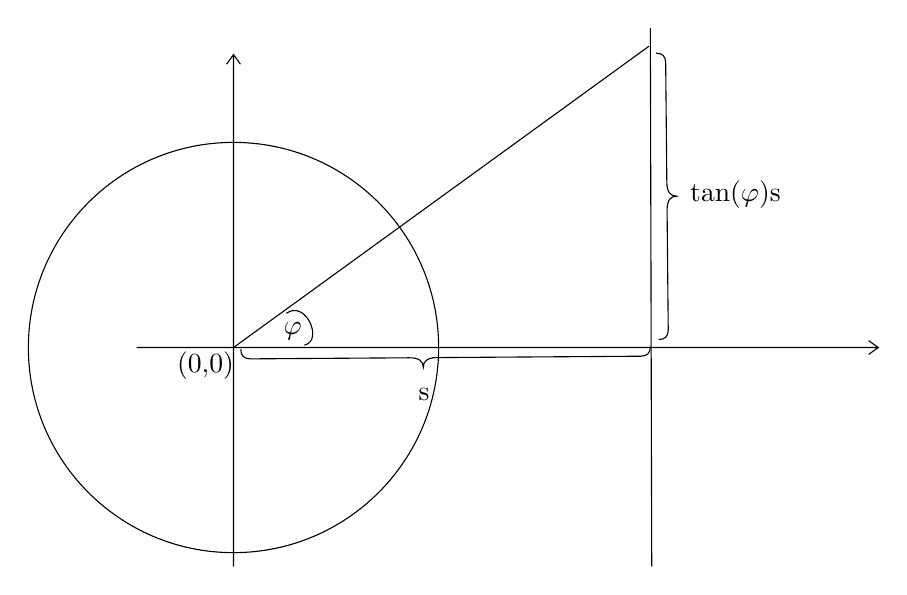
\begin{tikzpicture}[x=0.5pt,y=0.5pt,yscale=-1,xscale=1]
%uncomment if require: \path (0,444); %set diagram left start at 0, and has height of 444

%Shape: Axis 2D [id:dp6576255786763698] 
\draw  (100.32,236.75) -- (636.25,236.75)(170.25,25.01) -- (170.25,395.01) (629.25,231.75) -- (636.25,236.75) -- (629.25,241.75) (165.25,32.01) -- (170.25,25.01) -- (175.25,32.01)  ;
%Shape: Circle [id:dp3492792550747945] 
\draw   (22,236.57) .. controls (22.1,154.7) and (88.55,88.4) .. (170.43,88.5) .. controls (252.3,88.6) and (318.6,155.06) .. (318.5,236.94) .. controls (318.4,318.81) and (251.94,385.1) .. (170.06,385) .. controls (88.19,384.9) and (21.9,318.45) .. (22,236.57) -- cycle ;
%Straight Lines [id:da6321708159620955] 
\draw    (170.25,236.75) -- (470.5,19) ;


%Shape: Brace [id:dp4989740966069225] 
\draw   (175.5,238) .. controls (175.53,242.67) and (177.88,244.98) .. (182.55,244.95) -- (297.36,244.17) .. controls (304.03,244.12) and (307.37,246.43) .. (307.4,251.1) .. controls (307.37,246.43) and (310.69,244.08) .. (317.36,244.03)(314.36,244.05) -- (464.55,243.03) .. controls (469.22,243) and (471.53,240.65) .. (471.5,235.99) ;
%Curve Lines [id:da015330644298634621] 
\draw    (208.5,212) .. controls (222.5,202) and (235.5,232) .. (221.5,235) ;


%Shape: Brace [id:dp8380346617721155] 
\draw   (477.5,231) .. controls (482.17,230.95) and (484.48,228.6) .. (484.43,223.93) -- (483.6,137.43) .. controls (483.54,130.76) and (485.84,127.41) .. (490.51,127.37) .. controls (485.84,127.41) and (483.48,124.1) .. (483.41,117.43)(483.44,120.43) -- (482.58,30.93) .. controls (482.53,26.26) and (480.18,23.95) .. (475.51,24) ;
%Straight Lines [id:da8184237732199232] 
\draw    (471.5,6) -- (472.5,395) ;




\draw(150,250) node [align=left] {(0,0)};
% Text Node
\draw (308,271) node  [align=left] {s};
% Text Node
\draw (213,225) node  [align=left] {$\displaystyle \varphi $};
% Text Node
\draw (533,126) node  [align=left] {$\displaystyle \tan( \varphi )$s};
\end{tikzpicture}
\end{center}
Der Kreis ist ein zweidimensionaler Schnitt der Kugel. Es wird ein Punkt auf der rechten H\"alfte des Kreisrandes uniform gezogen (d. h. der Winkel $\varphi$ wird uniform aus $(-\frac{\pi}{2},\frac{\pi}{2})$ gezogen, $\varphi$ hat also Dichte $\frac 1 \pi \mathbf{1}_{(-\frac \pi 2, \frac \pi 2)}$). Dann wird der Laser vom Ursprung in Richtung des gezogenen Punktes auf dem Kreisrand geschossen und bis zur Mauer verl\"angert, wo dann ein bunter Punkt erscheint. Aus der Schule sollte noch bekannt sein, dass der Treffpunkt der Mauer $(s,\tan(\varphi)s)$ ist. Berechnen wir nun die Verteilung des Treffpunktes $Y$ ($y$-Achsen Abstand) auf der Mauer. Weil $\varphi\sim \mathcal U((-\frac{\pi}{2},\frac{\pi}{2}))$ ist, gilt
\begin{align*}
	\mathbb P(Y\leq t)=\mathbb P(\tan(\varphi) s\leq t)=\mathbb P(\varphi \leq \arctan(t/s))=\frac{1}{2}+\frac{1}{\pi}\arctan(t/s),
	\end{align*}
wobei in der letzten Gleichheit die Verteilungsfunktion von $\mathcal U((-\frac{\pi}{2},\frac{\pi}{2}))$ eingesetzt wurde (beachte, dass $\arctan(t/s)\in (-\frac{\pi}{2},\frac{\pi}{2})$ f\"ur alle $t,s\in\R$). Damit ist die Verteilungsfunktion von $Y$ gerade die Verteilungsfunktion von $\text{Cauchy}(s,0)$.
\end{beispiel}

Wir hatten angemerkt, dass die inverse Transformations Methode f\"ur die Normalverteilung nicht funktioniert weil $F^{-1}$ nicht explizit bekannt ist. Das n\"achste Beispiel ist daher ziemlich verbl\"uffend, die sogenante Box-Muller Methode. Man kann aus einer uniformen Zufallsvariable zwar nicht einfach eine normalverteilte Zufallsvariable bekommen, man kann aber ganz einfach aus zwei uniformen Zufallsvariablen zwei (und damit auch eine) normalverteilte bekommen! Sind $U_1, U_2$ unabh\"angige $\mathcal U([0,1])$ verteilte Zufallsvariablen, so sind 
\begin{align*}
	X_1=\cos(2\pi U_1) \sqrt{-\log(2U_2)}\quad \text{und}\quad
	X_2=\sin(2\pi U_1) \sqrt{-\log(2U_2)}
\end{align*}
zwei unabh\"angige $\mathcal N(0,1)$ Zufallsvariablen. Wer gerade noch Energie \"ubrig hat, kann mal versuchen, $\mathbb P(X_1\leq t_1,X_2\leq t_2)$ mit Polarkoordinaten auszurechnen (alle anderen k\"onnen sich das in der Monte Carlo Methoden Vorlesung anschauen). Um die Verteilung zu berechnen, solltet ihr euch an Korollar \ref{unabha} erinnern. Das Korollar besagt, dass $U_1,U_2$ und $X_1,X_2$ gemeinsame Dichten haben, n\"amlich jeweils das Produkt der einzelnen, also $\mathbf 1_{[0,1]\times [0,1]}$ bzw. $\frac{1}{2\pi} e^{-(x_1^2+x_2^2)/2}$. Damit wisst ihr, wie ihr $\mathbb P(X_1\leq t_1,X_2\leq t_2)$ durch Einsetzen der Definition ausrechnet und was rauskommen sollte.



\subsection{Summen von unabhängigen Zufallsvariablen}
Wir berechnen nun die Verteilungen von Summen unabhängiger Zufallsvariablen. Was ist zum Beispiel die Verteilung der Summe zweier exponentialverteilter Zufallsvariablen? Oder wie ist die Summe zweier Normalverteilungen verteilt? Allgemein ist das ziemlich schwierig zu sagen, wenn die Zufallsvariablen aber unabh\"angig sind, gibt es sch\"one Rechentricks.\smallskip

Starten wir mit dem diskreten Fall, der ist einfacher. Die Idee ist einfach: Durch welche Kombination von Werten, kann die Summe $X+Y$ einen gegebenen Wert annehmen? Nat\"urlich indem $Y$ irgendeinen Wert annimmt, und $X$ gerade die Differenz zum gegebenen Wert. Wenn man alle solche M\"oglichkeiten addiert (und die Unabh\"angigkeit ausnutzt), bekommt man die diskrete Faltungsformel:
\begin{satz}\label{diskreteFaltung}
\link{https://www.youtube.com/watch?v=wJVrIDI3kTQ&list=PLy5qRKPWp6SBwfc1kn-b66cWc84cOgvqZ&index=23&t=4502s} \textbf{[Diskrete Faltungsformel]}
	Sind $X,Y$ diskrete Zufallsvariablen auf $(\Omega, \cA, \mathbb{P})$, dann ist auch $X+Y$ diskret mit m\"oglichen Werten in $X(\Omega)+Y(\Omega):=\{a+b: a\in X(\Omega), b\in Y(\Omega)\}$. Dabei bezeichnen wir mit $X(\Omega), Y(\Omega)$ die m\"oglichen Werte von $X,Y$ sind. Sind $X$ und $Y$ unabh\"angig, so k\"onnen die Wahrscheinlichkeiten mit der Faltungsformel berechnet werden:
	\[ \mathbb{P}(X+Y = k) = \sum\limits_{b \in Y(\Omega)} \mathbb{P}(X = k-b) \mathbb{P}(Y=b),\quad k\in X(\Omega)+Y(\Omega).
	\]
\end{satz}
Lasst euch nicht von der komischen Notation mit den $X(\Omega)$ und $Y(\Omega)$ irritieren, man kann die Formel einfach nicht sch\"on hinschreiben. Sobald ihr euch die folgenden Beispiele angeschaut habt, ist ganz schnell alles klar.
\begin{proof}
	Dass die Summe diskret ist und als Werte gerade Summen der Werte von $X$ und $Y$ annehmen kann, ist hoffentlich klar (denkt an zwei W\"urfel). Der Trick f\"ur die Faltungsformel ist, ein diskretes Ereigniss in eine disjunkte Vereinigung von Teilereignissen (alle M\"oglichkeiten) zu zerlegen und darauf die $\sigma$-Additivit\"at anzuwenden. Wir schreiben den Beweis einmal knapp auf, so schreibt man Argumente mit diskreten Zufallsvariablen fast immer auf, und dann noch einmal super ausf\"uhrlich, um die Ma\ss theorie dahinter zu erkennen:	
		\begin{align*}
		\mathbb{P}(X+Y = k)	
		\overset{\sigma\text{-add.}}&{=} \sum\limits_{b \in Y(\Omega)} \mathbb{P}( X + Y = k, Y = b)\\ 
		&= \sum\limits_{b \in Y(\Omega)} \mathbb{P}( X = k-b, Y = b )\\
		 \overset{\text{unab.}}&{=} \sum\limits_{b \in Y(\Omega)} \mathbb{P}(X=k-b) \mathbb{P}(Y=b).
	\end{align*}
	Die zweite Gleichheit nutzt $\sigma$-Additivit\"at weil alle M\"oglichkeiten von $Y$ ausprobiert wurden. Ganz ausf\"uhrlich sieht das gleiche Argument wie folgt aus:	
	\begin{align*}
		\mathbb{P}(X+Y =k) \overset{\text{Notation}}&{=} \mathbb{P}(\{ \omega\colon X(\omega) + Y(\omega) = k \}) \\
		\overset{\text{Trick}}&{=} \mathbb{P}\Big(\bigcupdot_{b \in Y(\Omega)} \{ \omega\colon X(\omega) + Y(\omega) = k, Y(\omega) = b \} \Big)\\
		\overset{\sigma\text{-add.}}&{=} \sum\limits_{b \in Y(\Omega)} \mathbb{P}(\{ \omega\colon X(\omega) + Y(\omega) = k, Y(\omega) = b \})\\ 
		&= \sum\limits_{b \in Y(\Omega)} \mathbb{P}(\{ \omega\colon X(\omega) = k - b, Y(\omega) = b \})\\
		\overset{\text{Notation}}&{=} \sum\limits_{b \in Y(\Omega)} \mathbb{P}(X = k - b, Y = b )\\
		 \overset{\text{unab.}}&{=} \sum\limits_{b \in Y(\Omega)} \mathbb{P}(X=k-b) \mathbb{P}(Y=b).
	\end{align*}
	Wir m\"ussen in der Mathematik immer vorsichtig sein, einfache Dinge nicht zu sehr zu verkomplizieren. Diskrete Zufallsvariablen sind ganz sicher so ein Beispiel!
\end{proof}
Als Anmerkung zum Freuen auf die strahlende Zukunft: Genau wegen dieses kleinen Tricks, kann man so sch\"on mit Markovketten rumrechnen!\smallskip

Die Formel sieht vielleicht abstrakt und unhandlich aus, wie k\"onnen aber wirklich ganz einfach in konkrete Beispielen damit rechnen:



\begin{beispiel}
\link{https://www.youtube.com/watch?v=wJVrIDI3kTQ&list=PLy5qRKPWp6SBwfc1kn-b66cWc84cOgvqZ&index=23&t=4899s}
	Sind $X_1,...,X_n$ u.i.v mit $X_1 \sim \operatorname{Ber}(p)$ f\"ur ein $p\in (0,1)$, dann gilt $X_1+...+X_n \sim \operatorname{Bin}(n,p)$. Interpretation: Wenn $\operatorname{Ber}(p)$ die erfolgreiche Ausf\"uhrung eines Versuchs ($1$=Erfolg, $0$=Misserfolg) beschreibt, so beschreibt $\operatorname{Bin}(n,p)$ die Anzahl der erfolgreichen Ausf\"uhrungen von $n$ unabhängigen Versuchen.
\end{beispiel}

\begin{proof}
	Induktion über $n$:
	\begin{itemize}
		\item[IA:] $n=1$: $\checkmark$ $\operatorname{Ber}(p) = \operatorname{Bin}(1,p)$ nach Definition beider Verteilungen.
		\item[IV:] Die Behauptung gelte für ein \textit{beliebiges}, aber festes $n \in \N$.
		\item[IS:] Indem wir $X_1+...+X_{n+1}=(X_1+...+X_n)+X_{n+1}$ klammern, wenden wir die diskrete Faltungsformel an und nutzen dann die Induktionsvoraussetzung:
		 \begin{align*}
			\mathbb{P}(X_1+...+X_{n+1} = k)
			\overset{\text{\ref{diskreteFaltung}}}&{=} \mathbb{P}(X_1+...+X_{n} = k-1) \mathbb{P}(X_{n+1} = 1)\\
			&\quad + \mathbb{P}(X_1+...+X_{n} = k) \mathbb{P}(X_{n+1} = 0)\\
			&= \left(  n\atop{k-1}\right) p^{k-1} (1-p)^{n-k+1}p + \left( n\atop k\right) p^{k} (1-p)^{n-k}(1-p) \\
			&= \left(\left( n\atop {k-1} \right) + \left( n\atop  k\right)\right) p^k (1-p)^{n-k+1}\\
			& = \left({n + 1}\atop  k \right) p^k (1-p)^{n-k+1}.
		\end{align*}
		Im letzten Schritt haben wir eine Rechnenregel f\"ur Binomialkoeffizienten benutzt, die kennt ihr vermultich aus Analysis 1. Also ist $X_1+...+X_n \sim \operatorname{Bin}(n,p)$ gezeigt. 
	\end{itemize} 
\end{proof}
\begin{beispiel}
\link{https://www.youtube.com/watch?v=wJVrIDI3kTQ&list=PLy5qRKPWp6SBwfc1kn-b66cWc84cOgvqZ&index=23&t=5571s}
	Seien $X \sim \operatorname{Poi}(\lambda), Y \sim \operatorname{Poi}(\beta)$ unabhängig. Dann ist auch $X+Y$ Poissonverteilt, und zwar mit Parameter $\lambda+\beta$. In den \"Ubungen setzt ihr einfach in die Faltungsformel ein, um $X+Y\sim \operatorname{Poi}(\lambda+\beta)$ zu zeigen. Easy.
%	\begin{align*}
%		\mathbb{P}(X+Y=n) &= \sum\limits_{k \in \N_0} \mathbb{P}(X = n-k)\mathbb{P}(Y = k)\\
%		& = \sum\limits_{k=0}^{n} e^{-\lambda} \frac{\lambda^{n-k}}{(n-k)!} e^{-\beta} \frac{\beta^{k}}{k!}\\
%		&= e^{-(\lambda + \beta)} \frac{1}{n!} \sum\limits_{k=0}^{n} \frac{n!}{(n-k)!} \lambda^{n-k} \beta^{k}\\
%		& = e^{-(\lambda + \beta)} \frac{1}{n!} \sum\limits_{k=0}^{n} \Big(\begin{array}{c} n\\ k\end{array}\Big) \lambda^{n-k} \beta^{k}\\
%		& \overset{\text{bin.}}{\underset{\text{Formel}}{=}} e^{-(\lambda + \beta)} \frac{(\lambda + \beta)^n}{n!}.
%	\end{align*}
%	Damit ist $X+Y\sim \operatorname{Poi}(\lambda+\beta)$ gezeigt.
\end{beispiel}

\begin{deff}\link{https://www.youtube.com/watch?v=wJVrIDI3kTQ&list=PLy5qRKPWp6SBwfc1kn-b66cWc84cOgvqZ&index=23&t=5954s} \abs

\begin{itemize}
\item[(i)]
	Sind $\mu_1,...,\mu_n$ Wahrscheinlichkeitsmaße auf $\cB(\R)$, so heißt das Bildmaß vom Produktmaß $\mu_1 \otimes ... \otimes \mu_n$ unter der Abbildung $h_d(x_1,...,x_d) = x_1+...+x_d$ \textbf{Faltung} der Maße. Wir schreiben $\mu_1 *...* \mu_n$ für die Faltung.
%	\begin{center}		
%		\begin{tikzcd}
%			(\cB(\R^d), \mu_1 \otimes ... \otimes \mu_n) \arrow[r, "{h_d}"] & (\cB(\R), \mu_1 \times ... \times \mu_n).
%		\end{tikzcd}
%	\end{center}
\item[(ii)]
	Sind $X_1,...,X_d$ unabhängige Zufallsvariablen auf $(\Omega, \cA, \mathbb{P})$, so heißt $\mathbb{P}_{X_1} *...*\mathbb{P}_{X_d}$ \textbf{Faltung} von $X_1, ..., X_d$.
	\end{itemize}
\end{deff}

\begin{bem1}
	Nat\"urlich ist die Definition der Faltung abstrakt, andererseits ist sie auch konkret. Die Faltung ist nichts weiter als die Verteilung der Summe unabh\"angiger Zufallsvariablen:
	\begin{align*}
		X_1+...+X_n\sim \mathbb{P}_{X_1} *...*\mathbb{P}_{X_d}.
	\end{align*}	
	Wir m\"ussen uns daf\"ur nur daran erinnern, dass die Verteilung unabh\"angiger Zufallsvariablen das Produktma\ss{} ist:
	\begin{align*}
		\mathbb{P}(X_1+...+X_d \in B) &= \mathbb{P}(X_1,...,X_d \in h_d^{-1}(B)) \\
		\overset{\text{unab.}}&{=} \mathbb{P}_{X_1} \otimes ... \otimes \mathbb{P}_{X_d}(h_d^{-1}(B))\\
		\overset{\text{Def. push-forw.}}&{=} \mathbb{P}_{X_1} *...*\mathbb{P}_{X_d}(B).
	\end{align*}
\end{bem1}
Mit der Definition der Faltung k\"onnen wir erstmal nicht viel anstellen, wir haben die Faltung schlie\ss lich einfach als das definiert, was wir berechnen wollen. Was wir gerne h\"atten, w\"are ein analog zu der diskreten Faltungsformel, weil wir damit in konkreten Beispielen rechnen k\"onnen. Hier ist die allgemeine Formel, danach konkretisieren wir diese f\"ur den Fall mit Dichten.
\begin{prop}\label{randomProp}
\link{https://www.youtube.com/watch?v=wJVrIDI3kTQ&list=PLy5qRKPWp6SBwfc1kn-b66cWc84cOgvqZ&index=23&t=6597s}
	Seien $\mu_1,\mu_2$ Wahrscheinlichkeitsmaße auf $\cB(\R)$ mit Verteilungsfunktionen $F_1,F_2$, dann gelten:
	\begin{enumerate}[label=(\roman*)]
		\item Mit $B-y: = \{ x-y\colon x \in B \}$, d. h. die Verschiebung der Menge $B$ um $y$ nach links, gilt \[ \mu_1 * \mu_2(B) = \int_{\R} \mu_1(B-y) \dint \mu_2(y)\] f\"ur alle $B\in \mathcal B(\R)$.
		\item F\"ur alle $t\in \R$ gilt \[ F_{\mu_1 * \mu_2}(t) = \int_{\R} F_1(t-y) \dint \mu_2(y).\]
	\end{enumerate}
\end{prop}
\"Uberlegt mal kurz zum Spa\ss{}, warum die verschobenen Mengen $B-y$ wieder messbar sind. \footnote{Weil $B-y$ das Urbild von B unter der messbaren (weil stetig) Abildung $z\mapsto z+y$ ist.}
\begin{proof}\abs
	\begin{enumerate}[label=(\roman*)]
		\item 
		Wegen der Manipulation
		 \[ \mathbf{1}_{B-y}(x) = \begin{cases}
		1&:x \in B-y\\
		0&:\text{sonst}
		\end{cases} = \begin{cases}
		1&: x+y \in B\\
		0&: \text{sonst}
		\end{cases} = \mathbf{1}_{h_2^{-1}(B)}(x,y) \]
		folgt
		\begin{align*}
		\mu_1 * \mu_2(B) \overset{\text{Def.}}&{=} \mu_1 \otimes \mu_2(h_2^{-1}(B)) \\
		&= \int_{\R^2} \mathbf{1}_{h_2^{-1}(B)}(x,y) \dint \mu_1\otimes \mu_2(x,y)\\
		& = \int_{\R^2} \mathbf{1}_{B-y}(x) \dint \mu_1\otimes \mu_2(x,y) \\
		\overset{\text{Fubini}}&{=} \int_{\R} \Big( \int_{\R} \mathbf{1}_{B-y}(x) \dint \mu_1(x) \Big) \mu_2(y)\\
		& = \int_{\R} \mu_1(B-y) \dint \mu_2(y).
		\end{align*}
		Das ist die erste Aussage.
		\item Wir setzten in (i) die Mengen $B = (-\infty,t]$ mit $B-y = (-\infty,t-y]$ ein, und nutzen die Definition der Verteilungsfunktion.
	\end{enumerate}
\end{proof}
Nun zur konkreten Rechenvorschrift, um die Verteilung der Summe unabh\"angiger Zufallsvariablen mit Dichten zu berechnen:
\begin{satz}
\link{https://www.youtube.com/watch?v=wJVrIDI3kTQ&list=PLy5qRKPWp6SBwfc1kn-b66cWc84cOgvqZ&index=23&t=7199s} \textbf{[Stetige Faltungsformel]}
	Sind $X,Y$ unabhängige absolutstetige Zufallsvariablen mit Dichten $f_X$, $f_Y$, dann ist auch $X+Y$ absolutstetig und hat Dichte 
	\[ f_{X+Y}(x) = \int_{\R} f_X(x-y)f_Y(y) \dint y, \quad x\in\R.\]
\end{satz}
\begin{proof}
	Mit vorheriger Proposition kennen wir die Verteilungsfunktion der Summe. Wir rechnen diese mit der Formel aus und setzen dabei die bekannten Dichten ein:
	\begin{align*}
		\mathbb{P}_{X+Y}((-\infty,t])\overset{\text{Def. Faltung}}&{=}\mathbb{P}_X * \mathbb{P}_Y((-\infty,t])\\
		 \overset{\text{\ref{randomProp}}}&{=} \int_{\R} \mathbb{P}_X ((-\infty,t-y]) \dint \mathbb{P}_Y(y) \\
		\overset{\text{\ref{IntDichten}}}&{=} \int_{\R} \int_{-\infty}^{t-y} f_X(x) \dint x f_Y(y) \dint y\\
		 \overset{\text{Subst.}}&{=} \int_{\R} \int_{-\infty}^{t} f_X(x-y) \dint x f_Y(y) \dint y\\
		&= \int_{\R} \int_{\R} \mathbf{1}_{(-\infty,t]}(x) f_X(x-y) f_Y(y) \dint x \dint y\\
		 \overset{\text{Fubini}}&{=} \int_{-\infty}^{t} \int_{\R} f_X(x-y) f_Y(y) \dint y \dint x\\
		&= \int_{-\infty}^t f_{X+Y}(x)\dint x.	
	\end{align*}
	Also ist $X+Y$ absolutstetig mit behaupteter Dichte $f_{X+Y}$.
\end{proof}

	Das Konzept der Faltung kommt nicht aus der Stochastik, daher k\"onnen wir mit dem Begriff \enquote{Faltung} auch nichts anfangen. Die Faltung zweier integrierbarer Funktionen wird in der Fourieranalysis als 
	\begin{align*}
		f\ast g (x)=\int_\R f(x-y) g(y)\dint y,\quad x\in\mathbb R,
	\end{align*}
	definiert und zum Beispiel in der Signalverarbeitung studiert. Dass die Faltung bei uns f\"ur Summen unabh\"angiger Zufallsvariablen auftaucht, ist ein Zufall der Mathematik. Es gibt also keinen Grund sich Gedanken \"uber die Begrifflichkeit Faltung zu machen, f\"ur uns ist es einfach nur eine Berechnungsformel.
\marginpar{\textcolor{red}{Vorlesung 23}}



\begin{beispiel}\label{B5} \link{https://www.youtube.com/watch?v=lxTw3_a68yw&list=PLy5qRKPWp6SBwfc1kn-b66cWc84cOgvqZ&index=24&t=0s} \abs

	\begin{enumerate}[label=(\roman*)]\label{bspFaltung}
		\item Sind $X_1 \sim \cN(\mu_1,\sigma_1^2)$ und $X_2 \sim \cN(\mu_2,\sigma_2^2)$ unabhängig, dann ist auch die Summe wieder normalverteilt, genauer, es gilt $X_1 + X_2 \sim \cN(\mu_1 + \mu_2, \sigma_1^2 + \sigma_2^2)$. Das kann man mit der stetigen Faltungsformel ausrechnen:
		\begin{align*}
			f_{X_1 + X_2}(x) &= \int_{\R} \frac{1}{\sqrt{2 \pi \sigma_1^2}} e^{-\frac{(x-y-\mu_1)^2}{2\sigma_1^2}} \frac{1}{\sqrt{2 \pi \sigma_2^2}} e^{-\frac{(y-\mu_2)^2}{2\sigma_2^2}} \dint y\\
			&=\frac{1}{\sqrt{2\pi(\sigma_1^2+\sigma_2^2)}} e^{-\frac{(x-(\mu_1+\mu_2))^2}{2(\sigma_1^2+\sigma_2^2)}},\quad x\in\R.
		\end{align*}
		Auf den ersten Blick ist nicht so klar, ob die Berechnung einfach oder nicht so einfach ist. Im Prinzip muss man nur richtig quadratisch erg\"anzen und Substituieren. In der Tat ist die Rechnung ziemlich b\"ose, klappt aber. Weil wir gleich eine viel einfachere Methode kennenlernen, lassen wir die Rechnung weg.
		\item Sind $X_1 \sim \operatorname{Exp}(\lambda), X_2 \sim \operatorname{Exp}(\lambda)$ unabhängig, so ist $X_1+ X_2 \sim \Gamma(2,\lambda)$. Das kann man direkt mit der stetigen Faltungsformel ausrechnen:
		\begin{align*}
			f_{X_1+X_2}(x)&=\int_\R  f_{X_1}(x-y) f_{X_2}(y)\dint y\\
			 &=\int_\R \mathbf 1_{[0,\infty)}(x-y) \lambda e^{-\lambda (x-y)} \mathbf 1_{[0,\infty)}(y) \lambda e^{-\lambda y}\dint y\\
			&=\lambda^2 \int_0^x e^{-\lambda x} \dint y=\lambda^2 x e^{-\lambda x}.
		\end{align*}
\end{enumerate}
\end{beispiel}

Jetzt noch eine ganz andere Methode zur Berechnung der Verteilung der Summe von unabh\"angigen Zufallsvariablen. Daf\"ur nutzen wir einen Satz der Wahrscheinlichkeitstheorie, den Eindeutigkeitssatz f\"ur momenterzeugende Funktionen. Der Satz besagt, dass Verteilungen eindeutig durch ihre momenterzeugenden Funktionen festgelegt sind, falls diese um $0$ existieren.
\begin{satz}\label{WT}
\link{https://www.youtube.com/watch?v=lxTw3_a68yw&list=PLy5qRKPWp6SBwfc1kn-b66cWc84cOgvqZ&index=24&t=805s}
	Seien $X$ und $Y$ Zufallsvariablen f\"ur die die momenterzeugenden Funktionen $\cM_X,\cM_Y$ in $(-\varepsilon,\varepsilon)$ existieren für ein $\varepsilon > 0$. Falls $\cM_X(t) = \cM_Y(t)$ für alle $t \in (-\varepsilon,\varepsilon)$ gilt, so gilt $X\sim Y$.
	\end{satz}
\begin{proof}
	Siehe fortgeschrittene Stochastikvorlesung - hart!
\end{proof}
F\"ur Verteilungen mit expliziten momenterzeugenden Funktionen ist diese ein extrem n\"utzliches Hilfsmittel. 
\begin{beispiel}\label{B55}
\link{https://www.youtube.com/watch?v=lxTw3_a68yw&list=PLy5qRKPWp6SBwfc1kn-b66cWc84cOgvqZ&index=24&t=936s}
	Mit der momenterzeugenden Funktion k\"onnen wir ganz einfach die Skalierungseigenschaft der Normalverteilung zeigen: Ist $X\sim \mathcal N(0,1)$, $\mu\in \R$ und $\sigma^2>0$, so gilt $Y:=\sigma X+\mu \sim \mathcal N(\mu,\sigma^2)$. Rechnen wir dazu die momenterzeugende Funktion von $Y$ aus:
	\begin{align*}
		M_Y(t)=\E[e^{(\sigma X  + \mu)t}]=\E[e^{\sigma t X}]e^{\mu t}=M_{X}(\sigma t)\cdot e^{\mu t}= e^{\frac{\sigma^2 t^2}{2}+\mu t},\quad t\in \R,
	\end{align*}
	und die rechte Seite ist gerade die momenterzeugende Funktion einer $\mathcal N(\mu, \sigma^2)$-verteilten Zufallsvariable. Also folgt die Behauptung aus Satz \ref{WT}.
\end{beispiel}


Gemeinsam mit folgender Proposition ist Satz \ref{WT} ein m\"achtiges Hilfsmittel um die Verteilung Summen unabh\"angiger Zufallsvariablen zu berechnen:
\begin{prop}\label{P7}
\link{https://www.youtube.com/watch?v=lxTw3_a68yw&list=PLy5qRKPWp6SBwfc1kn-b66cWc84cOgvqZ&index=24&t=1375s}
	Sind $X$ und $Y$ unabhängige Zufallsvariablen mit $\cM_X(t),\cM_Y(t) < \infty$ f\"ur ein $t\in\R$, so gilt auch $\cM_{X+Y}(t) = \cM_X(t)\cM_Y(t)$.
\end{prop}

\begin{proof} 
Das folgt direkt daraus, dass Erwartungswerte von Produkten unabh\"angiger Zufallsvariablen faktorisieren, siehe Satz \ref{un}:
	$$\cM_{X+Y}(t) = \E[e^{t(X+Y)}] = \E[e^{tX}\cdot e^{tY}] = \E[e^{tX}] \cdot \E[e^{tY}] = \cM_X(t)\cM_Y(t).$$
\end{proof}

Die Anwendung der momenterzeugenden Funktion zur Bestimmung der Verteilung von Summen unabh\"angiger Zufallsvariablen versteht man am besten mit folgendem einfachen Beispiel. Beachte: Das Beispiel ist einfach, die Aussage aber nicht. H\"atten wir nicht die Kanone aus der Wahrscheinlichkeitstheorie ausgepackt, h\"atten wir das mit der stetigen Faltungsformel nachrechnen m\"ussen. 

\begin{beispiel}
\link{https://www.youtube.com/watch?v=lxTw3_a68yw&list=PLy5qRKPWp6SBwfc1kn-b66cWc84cOgvqZ&index=24&t=1661s}
	Kommen wir zur\"uck zu Beispiel \ref{B5} (i) und berechnen mit der Proposition die momenterzeugende Funktion der Summe der zwei unabh\"angigen Normalverteilungen. Wegen Proposition \ref{P7} und der in den \"Ubungen berechneten Formel f\"ur die momenterzeugende Funktion einer Normalverteilung gilt
	\begin{gather*}
		\cM_{X_1+X_2}(t) = \cM_{X_1}(t)\cM_{X_2}(t) = e^{\mu_1 t + \frac{\sigma_1^2}{2}t^2} e^{\mu_2 t + \frac{\sigma_2^2}{2}t^2}=e^{(\mu_1+\mu_2)t + \frac{\sigma_1^2 + \sigma_2^2}{2}t^2},\quad t\in\R.
	\end{gather*}
	Nun wissen wir aber auch, dass
	\begin{align*}
		\cM_Y(t)=e^{(\mu_1+\mu_2)t + \frac{\sigma_1^2 + \sigma_2^2}{2}t^2}, \quad t\in\R,
	\end{align*} 
	 f\"ur $Y \sim \cN(\mu_1 + \mu_2, \sigma_1^2 + \sigma_2^2)$. Also gilt $X_1+X_2\sim Y$ nach Satz \ref{WT} und damit gilt f\"ur die Summe $X_1+X_2\sim \mathcal N(\mu_1+\mu_2,\sigma_1^2 + \sigma_2^2)$.
\end{beispiel}
Mit \"ahnlichen Rechnungen kann man (siehe \"Ubungen) mit momenterzeugenden Funktionen auch zeigen, dass
\begin{itemize}
	\item die Summe unabh\"angiger Exponentialverteilungen gammaverteilt ist,
	\item die Summe unabh\"angiger Gammaverteilungen wieder gammaverteilt ist,
	\item die Summe unabh\"angiger Bernoulliverteilungen binomialverteilt ist (haben wir oben schon mit der Faltungsformel berechnet),
\end{itemize}
Das Argument ist immer identisch: Berechne die momenterzeugende Funktion der Summe als Produkt der momenterzeugenden Funktionen der einzelnen (Unabh\"angigkeit) und hoffe, dass das Produkt eine bereits bekannt momenterzeugende Funktion ist. Dann kann die Verteilung der Summe mittels Satz \ref{WT} identifiziert werden. 
\begin{bem}
\link{https://www.youtube.com/watch?v=lxTw3_a68yw&list=PLy5qRKPWp6SBwfc1kn-b66cWc84cOgvqZ&index=24&t=2038s}
\abs
\begin{itemize}
\item Der Trick mit der Normalverteilung funktioniert aufgrund der Faktorisierungseigenschaft der Exponentialfunktion. Wir sehen also, dass der Trick auf Situationen beschr\"ankt ist, wenn in einer n\"utzlichen Form Potenzen auftauchen. 
\item Die Vorlesung ist hier etwas irref\"uhrend. Satz \ref{WT} ist kein Allheilmittel. In der (mathematischen) Realit\"at sind exponentielle Momente sehr oft unendlich und wir k\"onnen nicht mit der momenterzeugenden Funktion arbeiten. In dieser Vorlesung sind alle Verteilungen au\ss er Cauchy und Exponentiell unproblematisch, weil alle exponentiellen Momente existieren. In der Wahrscheinlichkeitstheorie werden wir das Problem l\"osen, indem wir die Momenterzeugende Funktionen durch sogenannte charakteristische Funktionen $\varphi(t)=\E[e^{itX}]$ ersetzen. 
\end{itemize}
\end{bem}


\section{Bedingte Wahrscheinlichkeiten und Unabhängigkeit}\label{Sunab}
Wir kommen nun zu bedingten Wahrscheinlichkeiten, die aus der Schule vielleicht bekannt sind. In dieser Vorlesung spielen bedingte Wahrscheinlichkeiten noch keine zentrale Rolle, das \"andert sich in sp\"ateren Vorlesungen sehr, wenn zum Beispiel Markovketten angeschaut werden.
\begin{deff}
\link{https://www.youtube.com/watch?v=lxTw3_a68yw&list=PLy5qRKPWp6SBwfc1kn-b66cWc84cOgvqZ&index=24&t=2237s}
	Sei $(\Omega, \cA, \mathbb P)$ ein Wahrscheinlichkeitsraum und $A, B \in \cA$ mit $ \mathbb P(B)> 0$. Dann heißt \[ \mathbb{P}(A|B) := \frac{\mathbb{P}(A \cap B)}{\mathbb{P}(B)}\]
	\textbf{bedingte Wahrscheinlichkeit von $A$ gegeben $B$}.	
\end{deff}

\begin{lemma}
\link{https://www.youtube.com/watch?v=lxTw3_a68yw&list=PLy5qRKPWp6SBwfc1kn-b66cWc84cOgvqZ&index=24&t=2334s}
	Für $ B \in \cA$ mit $ \mathbb{P}(B)> 0$ ist $ A \mapsto \mathbb{P}(A|B) =: \mathbb{P}_B(A)$ ein Maß auf $(\Omega, \cA)$.
\end{lemma}

\begin{proof}
	Wir rechnen die definierenden Eigenschaften eines Ma\ss es nach:
	\begin{itemize}
		\item $\mathbb P_B(A) \geq 0$ f\"ur alle $A\in \mathcal A$ ist klar, weil $\mathbb P$ ein Ma\ss{} ist.
		\item Weil $\mathbb P$ ein Ma\ss{} ist, gilt auch 
		\[ \mathbb{P}_B(\emptyset) = \mathbb{P}(\emptyset|B) = \frac{\mathbb{P}(\emptyset \cap B)}{\mathbb{P}(B)} = 0. \]
		\item $\sigma$-Additivität: Seien $A_1,A_2,... \in \cA$ disjunkt, so gilt wegen der $\sigma$-Additivit\"at von $\mathbb P$
		\begin{align*}
			\mathbb{P}_B\big(\bigcupdot_{k=1}^{\infty} A_k \big) \overset{\text{Def.}}&{=} \frac{\mathbb{P}\big(\bigcupdot_{k=1}^{\infty} A_k \cap B\big)}{\mathbb{P}(B)}\\
			&= \frac{\mathbb{P}\big(\bigcupdot_{k=1}^{\infty} (A_k \cap B) \big)}{\mathbb{P}(B)} \\
			\overset{\sigma\text{-Add. }}&{=} \frac{\sum\limits_{k=1}^{\infty} \mathbb{P}(A_k \cap B)}{\mathbb{P}(B)}
			= \sum\limits_{k=1}^{\infty} \mathbb{P}_B(A_k).
		\end{align*}
	\end{itemize}
\end{proof}
Wir kommen nun zu extrem wichtigen Rechenregeln, obwohl diese ganz einfach aus der Definition folgen:
\begin{satz} \link{https://www.youtube.com/watch?v=lxTw3_a68yw&list=PLy5qRKPWp6SBwfc1kn-b66cWc84cOgvqZ&index=24&t=2512s} \abs

	\begin{enumerate}[label=(\roman*)]
		\item \label{multipl} \textbf{Multiplikationsregel}: Für $A_1,...,A_n\in \mathcal A$ mit $\mathbb{P}(\bigcap_{k=1}^{n} A_k) > 0$ gilt
		\[ \mathbb{P}\Big(\bigcap_{k=1}^{n} A_k\Big) = \mathbb{P}(A_1)\cdot \mathbb{P}(A_2|A_1)\cdot ... \cdot \mathbb{P}\Big(A_n\Big|\bigcap_{k=1}^{n-1} A_k\Big). \]
		\item \label{totWk} \textbf{Formel der totalen Wahrscheinlichkeit}: Ist $B_1,...,B_n\in \mathcal A$ eine disjunkte Zerlegung von $\Omega$, \mbox{d. h.}  $\bigcupdot_{k=1}^{n} B_k = \Omega$, mit $\mathbb P(B_k)>0$ f\"ur alle $k=1,...,n$, so gilt 
		\[ \mathbb{P}(A) = \sum\limits_{k=1}^{n} \mathbb{P}(B_k)\mathbb{P}(A|B_k), \quad \forall A \in \cA. \]
		\item \label{bayes} \textbf{Bayes-Formel}: Mit $B_1,...,B_n$ aus \ref{totWk} gilt für $A \in \cA$ mit $\mathbb{P}(A) > 0$ \[ \mathbb{P}(B|A) = \frac{\mathbb{P}(A|B) \cdot \mathbb{P}(B)}{\mathbb{P}(A)},\quad \forall B\in \mathcal A, \] oder \[ \mathbb{P}(B|A) = \frac{\mathbb{P}(A|B) \cdot \mathbb{P}(B)}{\sum\limits_{k=1}^{n} \mathbb{P}(B_k) \mathbb{P}(A | B_k)},\quad \forall B\in \mathcal A. \]
	\end{enumerate}
\end{satz}

\begin{proof}
	\begin{enumerate}[label=(\roman*)]
		\item Induktion über $n$:
		\begin{itemize}
			\item[IA:] $n=2$ folgt direkt aus der Definition der bedingten Wahrscheinlichkeit.
			\item[IV:] \label{IVmult} Die Behauptung gelte für ein \textit{beliebiges}, aber festes $n \in \N$.
			\item[IS:] Wenn wir nun die Induktionsvoraussetzung und den Fall $n=2$ nutzen, so bekommen wir 
			\begin{align*}
				\mathbb{P}\Big(\bigcap_{k=1}^{n+1} A_k\Big) &= \mathbb{P}\Big(\bigcap_{k=1}^{n} A_k\cap A_{n+1}\Big)\\
				& = \mathbb{P}\Big(\bigcap_{k=1}^{n} A_k\Big) \mathbb{P}\Big(A_{n+1}\Big |\bigcap_{k=1}^{n} A_k\Big)\\
				& \overset{\text{IV}}{=} \mathbb{P}(A_1)\cdot \mathbb{P}(A_2|A_1)\cdot ... \cdot \mathbb{P}\Big(A_{n+1}\Big|\bigcap_{k=1}^{n} A_k\Big)
			\end{align*}
			und das ist gerade die Aussage.
		\end{itemize}
		\item 
		Zun\"achst folgt direkt aus der Definition
		\begin{align*}
			\mathbb{P}(B_k)\mathbb{P}(A|B_k) = \mathbb{P}(B_k) \frac{\mathbb{P}(A \cap B_k)}{\mathbb{P}(B_k)} = \mathbb{P}(A \cap B_k).
		\end{align*}
		Setzen wir dies in folgende Rechnung ein, so bekommen wir die Aussage:
		\begin{align*}
			\mathbb{P}(A) = \mathbb{P}(A \cap \Omega) = \mathbb{P}\Big(A \cap \bigcupdot_{k=1}^{n} B_k\Big) = \mathbb{P}\Big(\bigcupdot_{k=1}^{n} (A \cap B_k)\Big)
			\overset{\sigma\text{-Add.}}{=} \sum\limits_{k=1}^{n} \mathbb{P}(A \cap B_k).
		\end{align*}
		\item Die einfache Bayes-Formel folgt direkt durch Einsetzen der Definition und Erweitern:
		\[ \mathbb{P}(B|A) = \frac{\mathbb{P}(A \cap B)}{\mathbb{P}(A)} = \frac{\mathbb{P}(A \cap B) \mathbb{P}(B)}{\mathbb{P}(B) \cdot \mathbb{P}(A)} =\frac{\mathbb{P}(A|B) \cdot \mathbb{P}(B)}{\mathbb{P}(A)} \]
		Ganz Aufmerksame werden merken, dass wir bei $\mathbb P(B)=0$ durch null geteilt haben. Das geht nat\"urlich nicht! Ist aber kein Problem, weil die Bayes-Formel in dem Fall als $0=0$ ohnehin gilt. Wir k\"onnen also ohne Einschr\"ankung $\mathbb P(B)>0$ annehmen und dann taucht das Problem nicht auf.\smallskip

		Die zweite Formel folgt aus der ersten Formel durch Ersetzen des Nenners durch die Formel der totalen Wahrscheinlichkeit. 
	\end{enumerate}
\end{proof}
Kommen wir nun zu zwei klassischen Anwendungen. Hier ist allerdings etwas Vorsicht angesagt, das ist alles etwas wild (funktioniert aber). Gem\"a\ss{} Definition brauchen wir f\"ur bedingte Wahrscheinlichkeiten einen Wahrscheinlichkeitsraum $(\Omega, \mathcal A, \mathbb P)$. In vielen Anwendungen au\ss erhalb der Mathematik werden die Formeln allerdings auch genutzt, ohne einen Wahrscheinlichkeitsraum hinzuschreiben. Nennen wir das vielleicht \enquote{heuristischen Gebrauch von Wahrscheinlichkeiten}. Das ist nat\"urlich nicht sehr sch\"on, allerdings sind solche Aussagen extrem wichtig. 

\begin{beispiel}\link{https://www.youtube.com/watch?v=lxTw3_a68yw&list=PLy5qRKPWp6SBwfc1kn-b66cWc84cOgvqZ&index=24&t=3627s} \abs

	\begin{enumerate}[label=(\roman*)]
		\item Wir ziehen aus vier blauen und drei weißen Kugeln zweimal ohne Zurücklegen. Was ist die Wahrscheinlichkeit, zwei blaue zu ziehen? Machen wir das ganze zun\"achst \enquote{heuristisch}. Das ist ein zweistufiges Experiment. Im ersten Versuch ziehen wir blau mit Wahrscheinlichkeit $\frac{4}{7}$. Mit dem Wissen im ersten Zug blau gezogen zu haben, ist das \enquote{bedingte Ziehen} im zweiten Schritt ein Ziehen aus drei blauen und drei wei\ss en Kugeln. Die bedingte Wahrscheinlichkeit im zweiten Schritt blau zu ziehen, gegeben das erste Ziehen gab eine blaue Kugel, ist also $\frac{3}{6}$. Mit der Multiplikationsregel folgt
		\begin{align*} 
		&\quad \mathbb{P}(\text{beide Kugeln blau}) \\
		&= \mathbb{P}(\text{erste Kugel blau}) \cdot \mathbb{P}(\text{zweite Kugel blau} \: | \: \text{erste Kugel blau})\\
		& = \frac{4}{7}\cdot \frac{3}{6} = \frac{2}{7}.
		\end{align*}
		Das funktioniert ganz entspannt, ist aber schon etwas kritisch. Wir nutzen hier ganz intuitiv den Begriff der bedingten Wahrscheinlichkeit in einem interpretierten Sinn (\"Anderung des Modells, eine Kugel weniger). Dann haben wir die Multiplikationsregel genutzt, die aufgrund unseres Beweises und damit aufgrund der mathematischen Definition der bedingten Wahrscheinlichkeit stimmt. Nun ist allerdings nicht so ganz klar, warum der intuitive Begriff der bedingten Wahrscheinlichkeit (ge\"andertes Experiment) mit der mathematischen Definition $\mathbb P(A\,|\,B):=\frac{\mathbb P(A\cap B)}{\mathbb P(B)}$ \"uberhaupt etwas zu tun hat. Machen wir das ganze zur Beruhigung also nochmal mathematisch penibel genau. Schreiben wir zun\"achst ein Modell hin, das wir als Modell f\"ur das zweifache W\"urfeln plausibel finden. Dazu sei
		$$\Omega = \{ (\omega_1,\omega_2)\colon \omega_1, \omega_2 \in \{ \text{blau, weiß} \} \}$$
		und $\cA = \cP(\Omega)$. Als Wahrscheinlichkeiten definieren wir
		\[ \mathbb{P}(\{ \omega_1, \omega_2 \}) = \begin{cases}
		\frac{4}{7} \cdot \frac{3}{6}&: \omega_1 = \omega_2 = \text{blau}\\
		\frac{3}{7} \cdot \frac{2}{6}&: \omega_1 = \omega_2 = \text{weiß}\\
		\frac{4}{7} \cdot \frac{3}{6}&: \omega_1 = \text{blau}, \: \omega_2 = \text{weiß}\\		
		\frac{3}{7} \cdot \frac{4}{6}&: \omega_1 = \text{weiß}, \: \omega_2 = \text{blau}\\
		\end{cases}. \]
		Mit den Ereignissen 		
		$A = \{ (\omega_1, \omega_2)\colon \omega_1 = \text{blau} \}$, $B = \{ (\omega_1, \omega_2)\colon \omega_2 = \text{blau} \}$
		wollen wir die Wahrscheinlichkeit von $A\cap B$ bestimmen. Mit der Multiplikationsregel folgt
		\begin{align*}
			\mathbb{P}(\text{ziehe zweimal blau}) = \mathbb{P}(A \cap B) = \mathbb{P}(A) \cdot \mathbb{P}(B|A) =  \frac{4}{7} \cdot \frac{\mathbb{P}(A \cap B)}{\mathbb{P}(A)} = \frac{2}{7}.
		\end{align*}
		Das macht nat\"urlich auch wieder nicht so richtig viel Sinn, wir h\"atten die Wahrscheinlichkeit von $A\cap B$ auch ohne die Multiplikationsregel \enquote{ablesen} k\"onnen. Dennoch ist das vielleicht eine gute Beruhigung: Wenn wir wollen, k\"onnen wir ein rigoroses Modell hinschreiben, in dem die Multiplikationsformel rigoros gemacht werden kann. F\"ur die Schulanwendungen ist das nat\"urlich viel zu kompliziert.		
		\item Nun ein Beispiel f\"ur die Bayes-Formel, ein medizinischer Test, \mbox{z. B.} ein Aidstest. Wir machen das jetzt wieder in der \enquote{heuristischen} Art, wer will, kann sich wieder ein sauberes Modell definieren. Wir nehmen an, dass die Wahrscheinlichkeiten folgender Ereignisse bekannt sind:
		\begin{itemize}
			\item $1\%$ der Bevölkerung ist tats\"achlich krank.
			\item Test ist mit $98\%$ positiv, wenn eine Person krank ist.
			\item Test ist mit $5\%$ positiv, wenn eine Person nicht krank ist, das nennt mann false-positive (Fehlalarm).
		\end{itemize}
		Gesucht ist die Wahrscheinlichkeit gesund zu sein, obwohl der Test positiv ist. Mit der Bayes-Formel gilt
		\begin{align*}
			&\quad \mathbb{P}(\text{krank} \: | \: \text{Test positiv})\\
			 &= \mathbb{P}(\text{Test positiv} \: | \: \text{krank}) \cdot \frac{\mathbb{P}(\text{krank})}{\mathbb{P}(\text{Test positiv})}\\
			&=	\frac{\mathbb{P}(\text{Test positiv} \: | \: \text{krank}) \mathbb{P}(\text{krank})}{\mathbb{P}(\text{Test positiv} \: | \: \text{krank})\mathbb{P}(\text{krank}) + \mathbb{P}(\text{Test positiv} \: | \: \text{gesund})\mathbb{P}(\text{gesund})}\\
			&= \frac{0,98 \cdot 0,01}{0,98 \cdot 0,01 + 0,05 \cdot 0,99} \\
			&= 0,165.
		\end{align*}
		Das ergibt dann
		\begin{align*}
			\mathbb{P}(\text{gesund} \: | \: \text{Test positiv}) = 1 - 0,165 = 0,835,
		\end{align*}
		was erschreckend hoch ist! Die wichtige take-home message ist also: Wird etwas sehr unwahrscheinliches getestet, dominieren falsche Tests und man muss bei positiven Tests unbedingt weitere Tests machen. Ein weiteres sehr wichtiges Beispiel sind pr\"anatale Tests bei ungeborenen Kindern, z. B. Tests auf Trisomie 21 (auf die moralische Frage wollen wir hier nat\"urlich nicht eingehen!).
	\end{enumerate}
\end{beispiel}
Weiter geht es jetzt mit einer mathematischen Definition von Unabh\"angigkeit von Ereignissen. Ihr habt sicherlich eine naive Vorstellung \glqq Hat nichts mit einander zu tun\grqq. Beispielsweise w\"aren die Ereignisse \enquote{Meine Kaffeemaschiene geht morgen kaputt} und \enquote{Es regnet morgen in Thailand} vermutlich unabh\"angig. Hier ist eine Definition:
\begin{deff}
\link{https://www.youtube.com/watch?v=lxTw3_a68yw&list=PLy5qRKPWp6SBwfc1kn-b66cWc84cOgvqZ&index=24&t=4799s}
	Sei $(\Omega, \cA, \mathbb{P})$ ein Wahrscheinlichkeitsraum und seien $A,B \in \cA$. Die Ereignisse $A$ und $B$ heißen \textbf{unabhängig}, falls $\mathbb{P}(A \cap B) = \mathbb{P}(A) \cdot \mathbb{P}(B)$.
\end{deff}
Aufgrund der Definition der bedingten Wahrscheinlichkeit sind, sofern $\mathbb P(B)>0$ gilt, $A$ und $B$ unabh\"angig genau dann, wenn $\mathbb P(A|B)=P(A)$. Das passt also zur Begriffsbildung: Zwei Ereignisse sind genau dann unabh\"angig, falls die Wahrscheinlichkeit des einen sich nicht \"andert, wenn das Eintreten des anderen gegeben ist.\smallskip

Oft braucht man auch die Unabh\"angigkeit mehrerer Ereignisse. F\"ur endlich viele ist klar was man macht, die Wahrscheinlichkeit des endlichen Schnittes soll nat\"urlich das endlich Produkt sein. F\"ur unendlich viele ist das problematisch, darum f\"uhrt man alles auf endlich viele zur\"uck:
\begin{deff}
\link{https://www.youtube.com/watch?v=lxTw3_a68yw&list=PLy5qRKPWp6SBwfc1kn-b66cWc84cOgvqZ&index=24&t=5109s}
	Sei $(\Omega, \cA, \mathbb{P})$ ein Wahrscheinlichkeitsraum, $A_i \in \cA$, $i \in I$, und $I$ eine beliebige Indexmenge.
	\begin{enumerate}[label=(\roman*)]
		\item Die Ereignisse ${(A_i)}_{i\in I}$ heißen \textbf{unabhängig}, falls 
		\[ \mathbb{P}\big(\bigcap_{i \in J} A_i \big) = \prod\limits_{i \in J} \mathbb{P}(A_i),\quad \forall J \subseteq I \text{ mit }  \# J<\infty. \]
		\item Die Ereignisse ${(A_i)}_{i\in I}$ heißen \textbf{paarweise unabhängig}, falls 
		$$\mathbb{P}(A_i \cap A_j) = \mathbb{P}(A_i) \cdot \mathbb{P}(A_j), \quad \forall i\neq j.$$
	\end{enumerate}
\end{deff}
Selbstverst\"andlich impliziert Unabh\"angikgkeit die paarweise Unabh\"angigkeit, statt aller endlicher Teilmengen $J$ von $I$ werden schlie\ss lich nur alle Teilmengen mit $\# J=2$ gew\"ahlt. Die Umkehrung gilt nicht:
\begin{warnung}
\link{https://www.youtube.com/watch?v=lxTw3_a68yw&list=PLy5qRKPWp6SBwfc1kn-b66cWc84cOgvqZ&index=24&t=5304s}
	Paarweise Unabhängigkeit impliziert im Allgemeinen nicht Unabhängigkeit. Kleine Mengen reichen schon aus, um Gegenbeispiel anzugeben, siehe \"Ubungsblatt.
\end{warnung}
In Worten ausgedr\"uckt hei\ss t die Unabh\"angigkeit auch \glqq Die Ereignisse ${(A_i)}_{i\in I}$ sind unabh\"angig, falls jede Wahl von endlich vielen Ereignissen $A_{i_1},...,A_{i_n}$ unabh\"angig ist\grqq.\smallskip

Als n\"achstes wollen wir die Unabh\"angigkeit von $\sigma$-Algebren und Zufallsvariablen thematisieren. Dazu zun\"achst eine allgemeinere Definition:
\begin{deff}\label{Ka}
\link{https://www.youtube.com/watch?v=lxTw3_a68yw&list=PLy5qRKPWp6SBwfc1kn-b66cWc84cOgvqZ&index=24&t=5374s}
	Sei $(\Omega, \cA, \mathbb{P})$ ein Wahrscheinlichkeitsraum und ${(\cE_i)}_{i \in I}$ eine Familie von Teilmengen $\cE_i \subseteq \cA$ der $\sigma$-Algebra f\"ur eine beliebige Indexmenge $I$. Dann heißen die $(\cE_i)_{i\in I}$ unabhängig, falls die Ereignisse ${(A_i)}_{i \in I}$ unabhängig sind, und zwar f\"ur alle $A_i \in \cE_i$.
\end{deff}


Die Definition wird insbesondere f\"ur $\sigma$-Algebren verwendet. Wie bei der Messbarkeit fragen wir uns hier, ob wir die Unabh\"angigkeit auf Erzeuger reduzieren k\"onnen. Wie immer funktioniert das, zumindest wenn der Erzeuger $\cap$-stabil ist:
\begin{prop}\label{unabh}
\link{https://www.youtube.com/watch?v=lxTw3_a68yw&list=PLy5qRKPWp6SBwfc1kn-b66cWc84cOgvqZ&index=24&t=5613s}
	Ist $(\Omega, \cA, \mathbb{P})$ ein Wahrscheinlichkeitsraum und $\cE_i \subseteq \cA$ für f\"ur alle $i \in I$. Sind alle $\cE_i$ $\cap$-stabil, so gilt:
	\begin{align*}
		(\cE_i)_{i\in I}\text{ unabhängig }\quad \Leftrightarrow\quad  (\sigma(\cE_i))_{i \in I}\text{ unabhängig.}
	\end{align*}
\end{prop}

\begin{proof}\abs
	\begin{itemize}
		\item[\enquote{$\Leftarrow$}:] Klar nach Definition, weil $\cE_i \subseteq \sigma(\cE_i)$ gilt. Die Unabh\"angigkeit von Mengensystemen bedeutet schlie\ss lich, dass die Unabh\"angigkeit f\"ur alle Auswahlen von Teilmengen gilt. Gilt dies f\"ur mehr M\"oglichkeiten, so nat\"urlich auch f\"ur weniger M\"oglichkeiten.
		\item[\enquote{$\Rightarrow$}:] Ohne Einschr\"ankung sei $I$ endlich weil die Definition der Unabh\"angkigkeit nur auf endlichen Teilmengen $J \subseteq I$ beruht. Nennen wir die Mengen $\cE_1,...,\cE_n$. Wir zeigen, dass dann auch $\sigma(\cE_1),...,\sigma(\cE_n)$ unabhängig sind. Dazu zeigen wir zun\"achst:
		$$\cD:= \big\{ E \in \cA \colon \{ E \}, \cE_2, ..., \cE_n \text{ sind unabhängig} \big\}\text{ ist ein Dynkin-System.}$$
		Um das zu zeigen, checken wir die definierenden Eigenschaften eines Dynkin-Systems:
		\begin{enumerate}[label=(\roman*)]
			\item Aufgrund der Definition \ref{Ka} m\"ussen wir zeigen, dass f\"ur alle $ A_2 \in \cE_2,...,A_n \in \cE_n$ die Mengen $\Omega, A_2,...,A_n$ unabhängig sind, die Wahrscheinlichkeit vom Schnitt also zur Wahrscheinlichkeiten der einzelnen Ereignisse faktorisiert. Das folgt aber direkt aus der angenommenen Unabh\"angigkeit von $\mathcal E_1, ..., \mathcal E_n$:			
			\begin{align*}
				\mathbb{P}(\Omega \cap A_2 \cap ... \cap A_n) &= \mathbb{P}(A_2 \cap ... \cap A_n)\\
				 &= \mathbb{P}(A_2) \cdot ... \cdot \mathbb{P}(A_n)\\
				 & = 1 \cdot \mathbb{P}(A_2) \cdot ... \cdot \mathbb{P}(A_n)
				  = \mathbb{P}(\Omega) \cdot \mathbb{P}(A_2) \cdot ... \cdot \mathbb{P}(A_n).
			\end{align*}
			Damit ist $\Omega \in \cD$.
			\item Nun zur Abgeschlossenheit bez\"uglich Komplementbildung. Wir argumentieren wie im ersten Schritt. Sei dazu $E \in \cD$ und seien $A_2 \in \cE_2,...,A_n \in \cE_n$ beliebig. Weil $\Omega=E\cupdot E^C$ ergibt sich
			\begin{align*}
				&\quad \mathbb{P}(E^C \cap A_2 \cap ... \cap A_n)\\
				 \overset{\sigma\text{-Add.}}&{=} \mathbb{P}(\Omega \cap A_2 \cap ... \cap A_n) - \mathbb{P}(E \cap A_2 \cap ... \cap A_n) \\
				\overset{\Omega, E\in \mathcal D}&{=} \mathbb{P}(\Omega) \cdot \mathbb{P}(A_2) \cdot ... \cdot \mathbb{P}(A_n) - \mathbb{P}(E) \cdot \mathbb{P}(A_2) \cdot ... \cdot \mathbb{P}(A_n)\\
				&= (\mathbb{P}(\Omega) - \mathbb{P}(E)) \cdot \mathbb{P}(A_2) \cdot ... \cdot \mathbb{P}(A_n)\\
				&= \mathbb{P}(E^C) \cdot \mathbb{P}(A_2) \cdot ... \cdot \mathbb{P}(A_n).
			\end{align*}
			Also sind $E^C, A_2, ...,A_n$ unabh\"angige Ereignisse und damit ist $E^C\in \cD$.
			\item Das Argument f\"ur die Vereinigungen geht genau wie f\"ur die Komplemente.
		\end{enumerate}
		Jetzt beenden wir den Beweis. Aufgrund der Annahme $\cE_1,...,\cE_n$ unabhängig, gilt f\"ur jede Menge $E\in \cE_1$ auch $E\in \cD$. Also gilt $\cE_1\subseteq \cD$. Daraus folgt mit dem Hauptsatz f\"ur Dynkinsysteme, Satz \ref{Hauptsatz}, wie immer (Bildung des kleinsten Dynkin-Systems ist monoton)
			\[ \sigma(\cE_1)\overset{\cap\text{-stabil}}{=}  d(\cE_1)\subseteq d(\cD) = \cD. \]			
			Weil also $\sigma(\cE_1)\subseteq \cD$ gilt, folgt aus der Definition von $\cD$, dass $\sigma(\cE_1), \cE_2,...,\cE_n$ unabhängig sind. Iterativ ersetzen wir nun Schritt f\"ur Schritt mit einem analogen Argument ein $\cE_k$ nach dem anderen durch $\sigma(\cE_k)$, indem wir genau wie oben zeigen, dass alle 
			\begin{align*}
				\cD_k:= \big\{ E \in \cA \colon \sigma(\cE_1), \sigma(\cE_2),... ,\sigma(\cE_{k-1}),\{E\}, \cE_{k+1}, ..., \cE_n \text{ sind unabhängig} \big\}
			\end{align*}
			Dynkin-Systeme sind und daraus $\sigma(\mathcal E_k)\subseteq \mathcal D_k$ folgern.
		\end{itemize}
\end{proof}
\marginpar{\textcolor{red}{Vorlesung 24}}
Nach der Unabh\"angigkeit von Ereignissen und Zufallsvariablen kommen wir nun zu einer alternativen Definition der Unabh\"angigkeit von Zufallsvariablen. Anstatt die Faktorisierung der gemeinsamen Verteilung zu fordern, kann man auch fordern, dass die erzeugten $\sigma$-Algebren (siehe Definition \ref{Kat}) unabh\"angig sind:
\begin{deff}\label{unab}
\link{https://www.youtube.com/watch?v=tJ-TYBzCFV8&list=PLy5qRKPWp6SBwfc1kn-b66cWc84cOgvqZ&index=25&t=34s}
	Für Zufallsvariablen $(X_i)_{i \in I}$ auf $(\Omega, \cA, \mathbb{P})$ definiert man: $(X_i)_{i \in I}$ sind unabhängig, falls die erzeugten $\sigma$-Algebren $(\sigma(X_i))_{i \in I}$ unabhängig sind. 
\end{deff}
Weil $\sigma(X_i) \overset{\text{Def.}}{=} \{ X_i^{-1}(B): B\in \mathcal B(\R)\}= \sigma(\{ X_i^{-1}((-\infty,t])\colon t \in \R \})$, k\"onnen wir direkt folgern, dass die Unabh\"angigkeit auch durch die gemeinsame Verteilungsfunktion definiert werden kann.
\begin{korollar}
\link{https://www.youtube.com/watch?v=tJ-TYBzCFV8&list=PLy5qRKPWp6SBwfc1kn-b66cWc84cOgvqZ&index=25&t=237s}
	Für Zufallsvariablen $X_1,...,X_d$ auf $(\Omega, \cA, \mathbb{P})$ stimmt die neue Definition der Unabh\"angigkeit mit der alten überein. Wir k\"onnen Unabh\"angigkeit also auf verschiedene Arten beschreiben:
	\begin{align*}
		&\quad X_1,...,X_d \text{ sind unabh\"angig}\\
		&\Leftrightarrow \quad \sigma(X_1),...,\sigma(X_d)\text{ sind unabh\"angige }\sigma\text{-Algebren}\\
		&\Leftrightarrow \quad F_X(t_1,...,t_d)=F_{X_1}(t_1)\cdot...\cdot F_{X_d}(t_d),\quad \forall t_i\in\R\\
		&\Leftrightarrow \quad \mathbb P(X_1\in A_1,...,X_d\in A_d)=\mathbb P(X_1\in A_1)\cdot ... \cdot \mathbb P(X_d\in A_d),\quad \forall A_i\in \mathcal B(\R).
	\end{align*}
\end{korollar}
\begin{proof}

Um die vorherige Proposition anzuwenden, seien $\cE_i := \{ \{X_i \leq t \}\colon t \in \R \}$ f\"ur $i=1,...,d$. Also gilt $\sigma(\cE_i) = \sigma(X_i)$ und die $\cE_i$ sind $\cap$-stabil. \"Uberlegen wir einmal schnell, warum $\sigma(\cE_i) = \sigma(X_i)$ gilt. Die Richtung \glqq$\subseteq$\grqq{} gilt, weil $\cE_i\subseteq \sigma(X_i)$ aufgrund der Definition von $\sigma(X_i)$. Die Richtung \glqq$\supseteq$\grqq{} gilt, weil wegen Proposition \ref{S2} $X_i$ $(\sigma(\cE_i),\mathcal B(\R))$-messbar ist und $\sigma(X_i)$ die kleinste $\sigma$-Algebra ist, bez\"uglich derer $X_i$ messbar ist.\smallskip

Damit gilt aufgrund der Definitionen der Unabh\"angigkeit von Mengensystemen und Ereignissen
\begin{align*}
	&\quad \sigma(X_1),...,\sigma(X_d) \text{ unabhängig }\\
	\overset{\ref{unabh}}&{\Leftrightarrow}\quad \cE_1,...,\cE_d \text{ unabhängig}\\
	&\Leftrightarrow\quad E_1,...,E_d \text{ unabh\"angig f\"ur alle } E_1\in \cE_1, ..., E_d\in \cE_d\\
	&\Leftrightarrow\quad \mathbb{P}(\{ X_1 \leq t_1 \} \cap ... \cap \{ X_d \leq t_d \})=\mathbb P(\{X_1\leq t_1\})\cdots \mathbb P(\{X_d\leq t_d\}),\quad t_1,..., t_d\in \R\\
		\overset{\text{Notation}}&{\Leftrightarrow}\quad \mathbb{P}( X_1 \leq t_1 , ... , X_d \leq t_d)=\mathbb P(X_1\leq t_1)\cdots \mathbb P(X_d\leq t_d),\quad t_1,..., t_d\in \R\\
	\overset{\text{Def. VF}}&{\Leftrightarrow} \quad F_X(t_1,..., t_d)=F_{X_1}(t_1)\cdots F_{X_d}(t_d),\quad t_1,..., t_d\in \R.
\end{align*}	
\end{proof}
Bitte beachtet die Notation im letzten Beweis. In der Stochastik bevorzugen wir immer die Notation
$\mathbb{P}( X_1 \leq t_1 , ... , X_d \leq t_d)$, wir nutzen praktisch nie die ausf\"uhrliche Schreibweise $\mathbb{P}(\{ X_1 \leq t_1 \} \cap ... \cap \{ X_d \leq t_d \})$. Das liegt einfach nur daran, dass sich die erste Notation viel nat\"urlicher lesen l\"asst. Am besten gew\"ohnt ihr euch direkt die kompakte Schreibweise an.\smallskip

Im n\"achsten Abschnitt besprechen wir Konvergenzen von Folgen von Zufallsvariablen. Wir werden insbesondere Folgen unabh\"angiger Zufallsvariablen nutzen. Unsere urspr\"ungliche Definition war nur f\"ur endlich viele Zufallsvariablen, die Definition dieses Abschnittes funktioniert auch f\"ur unendlich viele Zufallsvariablen (man testet die Eigenschaft einfach f\"ur alle endlichen Teilmengen). Genau so wollen wir ab jetzt die Unabh\"angigkeit einer ganzen Folgen von Zufallsvariablen definieren.
\begin{deff}
\link{https://www.youtube.com/watch?v=tJ-TYBzCFV8&list=PLy5qRKPWp6SBwfc1kn-b66cWc84cOgvqZ&index=25&t=815s}
	Ist $X_1,X_2,...$ eine (unendliche) Folge von Zufallsvariablen auf $(\Omega, \mathcal A, \mathbb P)$, so hei\ss t die Folge unabh\"angig, falls eine der \"aquivalenten Eigenschaften gilt: 
\begin{itemize}
\item[(i)] $\text{F\"ur alle } n\in\N\text{ sind }\sigma(X_1), ..., \sigma(X_n)\text{ unabh\"angige }\sigma\text{-Algebren}$.
\item[(ii)] $	\text{F\"ur alle } n\in\N\text{ gilt: } \mathbb P(X_1 \leq t_1, ..., X_n\leq t_n)=\prod_{k=1}^n \mathbb P(X_k \leq t_k),\quad t_1,...,t_n\in\R.$
\end{itemize}
\end{deff}
Wie f\"ur Zufallsvariablen und Zufallsvektoren ist es auch f\"ur Folgen von Zufallsvariablen nicht klar, dass es diese \"uberhaupt gibt. In der Tat kann man auch in diesem Fall eine kanonische Konstruktion angeben, die uns die Existenz von Folgen unabh\"angiger Zufallsvariablen gibt. Der kanonische Wahrscheinlichkeitsraum besteht ganz analog aus den Werten, die angenommen werden. Dies war zun\"achst $\R$, dann $\R^d$ und ist nun $\R^\infty$ (die Menge der reellen Folgen). Die kanonische $\sigma$-Algebra ist die passende \enquote{Borel}-$\sigma$-Algebra und die Folge der Zufallsvariablen ist durch die Identit\"atsabbildung gegeben. Das Thema geh\"ort eigentlich nicht in die Stochastik 1 sondern in die Wahrscheinlichkeitstheorie 1. Daher skizzieren wir die Konstruktion nur ganz kurz. Ihr solltet euch jedoch merken, dass es eine kanonische Konstruktion gibt und insbesondere Folgen von unabh\"angigen Zufallsvariablen existieren
\begin{satz}\label{Folge}
\link{https://www.youtube.com/watch?v=tJ-TYBzCFV8&list=PLy5qRKPWp6SBwfc1kn-b66cWc84cOgvqZ&index=25&t=1100s} \textbf{[Kanonische Konstruktion von Folgen unabhängiger Z.V.]}
	Seien $F_1,F_2,...$ Verteilungsfunktionen, so existieren ein Wahrscheinlichkeitsraum $(\Omega, \cA, \mathbb{P})$ und eine Folge \textit{unabhängiger} Zufallsvariablen $X_1,X_2,...$ auf $(\Omega, \cA, \mathbb{P})$ mit $X_i \sim F_i$.
\end{satz}


\begin{proof}
	Man kann ganz analog zu $\R$ und zum $\R^d$ eine kanonische Konstruktion angeben. Hier nur eine Skizze f\"ur die \"ubermotivierten Studis, die Konstruktion wird in Ruhe in einer der Vorlesungen im Master thematisiert. Alle anderen merken sich aber bitte die Aussage des Satzes, sonst w\"are die Vorlesung an dieser Stelle vorbei!
\begin{itemize}
\item $\Omega := \{ (\omega_n)_{n\in\N}\colon \omega_n \in \R \}$, die Menge der \enquote{reelle Folgen}. Die $\omega$ sind also Folgen, oder unendlich lange Vektoren. Als Analogie zum $\R^d$ schreibt man auch $\R^\infty$. 
\item $\cA:= \cB(\R^{\infty}) := \sigma(\{B_1\times ... \times B_d \times \R \times \R\times ... : d\in \N, B_1, ..., B_d \in \cB(\R) \})$
\item $\mathbb{P}: = \mathbb{P}_{F_1} \otimes \mathbb{P}_{F_2} \otimes ...$ sei das unendliche Produktma\ss, das auf dem Erzeuger von $\mathcal B(\R^\infty)$ festgelegt ist durch $\mu(B_1 \times ... \times B_d \times \R\times ...)=\mathbb P_{F_1}(B_1) \cdots \mathbb P_{F_d}(B_d)$.
\item $(X_1(\omega), X_2(\omega), ... ):=(\omega_1, \omega_2,...)=\omega$
\end{itemize}
Um zu zeigen, dass es ein unendliches Produktma\ss{} auf $(\R^\infty, \mathcal B(\R^\infty))$ auch gibt, kann man den Fortsetzungssatz von Carath\'eodory anwenden. Das ist etwas h\"asslich. Wir haben nun also einen Wahrscheinlichkeitsraum und eine Folge von Zufallsvariablen, die einfach nur f\"ur ein $\omega$ die Koordinaten ausgibt (genau wie im $\R^d$, vergleiche den Beweis von Satz \ref{kan}). Die Unabh\"angigkeit der konstruierten Folge folgt direkt aus der Produkteigenschaft des Produktma\ss es, weil aufgrund der Definition der Zufallsvariablen als Koordinatenabbildungen
\begin{align*}
	\mathbb P(X_{1}\leq t_1, ... ,X_{n}\leq t_n)
	\overset{\text{Def }X}&{=}\mathbb P((-\infty,t_1]\times...\times (-\infty,t_n] \times \R\times \R \times ...)\\
	\overset{\text{Produktma\ss}}&{=}\mathbb P_{F_{1}}((-\infty,t_1])\cdots \mathbb P_{F_{n}}((-\infty,t_n])\\
	&=\mathbb P(X_{1}\leq t_1)\cdots \mathbb P(X_{n}\leq t_n).
\end{align*}
 Auch sofort folgt durch Einsetzen, dass die Randverteilungen $\mathbb P(X_i\leq t)=F_{X_i}(t)$ erf\"ullen.
\end{proof}

\begin{deff}
\link{https://www.youtube.com/watch?v=tJ-TYBzCFV8&list=PLy5qRKPWp6SBwfc1kn-b66cWc84cOgvqZ&index=25&t=2360s}
	Sind alle $F_i$ gleich, so nennen wir die Folge unabh\"angiger Zufallsvariablen $X_1,X_2,...$ aus Satz \ref{Folge} eine u.i.v. Folge mit $X_1 \sim F_1$.
\end{deff}
In den n\"achsten Kapitel schauen wir uns Konvergenzeigenschaften von u.i.v Folgen an, insbesondere das Gesetz der gro\ss en Zahlen und den zentralen Grenzwertsatz.

\section{Konvergenz von Folgen von Zufallsvariablen}
Bevor wir zu den zentralen Konvergenzs\"atzen kommen, m\"ussen wir uns \"uberlegen, was Konvergenz von Folgen von Zufallsvariablen \"uberhaupt bedeutet. Das ist in der Tat gar nicht so klar, es gibt verschiedene Begriffe:
\begin{deff}
\link{https://www.youtube.com/watch?v=tJ-TYBzCFV8&list=PLy5qRKPWp6SBwfc1kn-b66cWc84cOgvqZ&index=25&t=2763s} \textbf{[Vier Konvergenzarten in der Stochastik]}
	Für eine Zufallsvariable $X$ und eine Folge $X_1,X_2,...$ von Zufallsvariablen auf $(\Omega, \cA, \mathbb{P})$  definiert man
	\begin{enumerate}[label=(\roman*)]
		\item \enquote{$X_n$ konvergiert \textbf{stochastisch} (oder \textbf{in Wahrscheinlichkeit}) gegen $X$}, man schreibt		
		$$X_n \overset{P}{\longrightarrow} X, \quad n \to \infty,$$ falls f\"ur alle $\varepsilon>0$ $$\mathbb{P}(|X_n-X|>\varepsilon) \to 0, \quad n \to \infty.$$
		\item \enquote{$X_n$ konvergiert \textbf{in $\mathcal L^p$} gegen $X$} (oder \textbf{im $p$-ten Mittel}) f\"ur $p\geq 1$, man schreibt
		$$X_n \overset{\cL^p}{\longrightarrow} X, \quad n \to \infty,$$ falls $$\E[|X_n - X|^p] \to 0, \quad n \to \infty.$$
		\item 
		\enquote{$X_n$ konvergiert \textbf{fast sicher} gegen $X$}, man schreibt
		$$X_n \overset{\text{f.s.}}{\longrightarrow} X, \quad n \to \infty,$$ falls $$\mathbb{P}(X_n \to X) := \mathbb{P}(\{ \omega\colon X_n(\omega) \to X(\omega), \: n\to \infty \}) = 1.$$
		\item 
		 \enquote{$X_n$ konvergiert  \textbf{in Verteilung} (oder \textbf{schwach}) gegen $X$}, man schreibt		
		$$X_n \overset{(d)}{\longrightarrow} X, \quad n \to \infty,$$ falls f\"ur \underline{alle} $f:\R\to\R$ stetig und beschr\"ankt
		$$\E[f(X_n)] \to \E[f(X)], \quad n\to\infty.$$
	\end{enumerate}
\end{deff}
Nur die ersten drei Konvergenzbegriffe ben\"otigen wirklich, dass die Zufallsvariablen auf dem selben Wahrscheinlichkeitsraum definiert sind. Die Konvergenz in Verteilung ist strukturell anders weil die Zufallsvariablen $X_n$ nicht direkt mit der Grenzzufallsvariablen $X$ \enquote{verglichen} werden, es wird nicht $|X_n(\omega)-X(\omega)|$ berechnet. Die Konvergenz in Verteilung h\"angt nur von den Verteilungen ab, vergleiche dazu die Berechnungsformel des Erwartungswertes mit dem Transformationssatz, Lemma \ref{ewTrafo}.
\begin{bem} \link{https://www.youtube.com/watch?v=tJ-TYBzCFV8&list=PLy5qRKPWp6SBwfc1kn-b66cWc84cOgvqZ&index=25&t=3240s} \abs
	\begin{enumerate}[label=(\roman*)]
		\item Warnung: Die Konvergenzen sind nicht durch Metriken definiert worden, \mbox{d. h.} \"ubliche Tricks aus der Analysis (z. B. $\triangle$-Ungleichung, Eindeutigkeit von Grenzwerten, ...) gelten nicht einfach so! Konkretes Beispiel: Nur wenn man einen Quotientenraum mit fast sicher gleichen Zufallsvariablen bildet, ist Konvergenz im $p$-ten Mittel eine Normenkonvergenz und die Eindeutigkeit von Grenzwerten gilt (siehe \"Ubungsaufgaben).
		\item Zwei Konvergenzarten sind uns schon bekannt:
		\begin{itemize}
			\item fast sichere Konvergenz ist schon von messbaren Funktionen bekannt,
			\item $p$-tes Mittel ist schon von $(\mathcal L^p, ||\cdot||_p)$ bekannt.
		\end{itemize}
	\end{enumerate}
\end{bem}

Um ein Gef\"uhl f\"ur die Konvergenzarten zu bekommen, sind Beispiele \"ausserst n\"utzlich. Viele n\"utzliche Beispiele k\"onnen ganz explizit hingeschrieben werden.
\begin{beispiel}
\link{https://www.youtube.com/watch?v=tJ-TYBzCFV8&list=PLy5qRKPWp6SBwfc1kn-b66cWc84cOgvqZ&index=25&t=3651s}
	Seien $X_1, X_2, ... $ Zufallsvariablen auf irgendeinem Wahrscheinlichkeitsraum $(\Omega, \mathcal A,\mathbb P)$ mit  $$\mathbb{P}(X_n = e^n) = \frac{1}{n}, \quad \mathbb{P}(X_n = 0) = 1 - \frac{1}{n},$$ so gelten:\smallskip
	
	$\mathbf{X_n \overset{P}{\longrightarrow} 0, n \to \infty},$ weil $$\mathbb{P}(|X_n - X| > \varepsilon) = \mathbb{P}(X_n = e^n)=\frac{1}{n}\to 0, \quad n\to\infty.$$
	
	$\mathbf{X_n \overset{\cL^p}{\not\longrightarrow} 0, n \to \infty}$, f\"ur alle $p\geq 1$, weil 
	$$\E[|X_n - X|^p] = \E[|X_n|^p] = e^{pn} \frac{1}{n} + 0^p\Big(1-\frac{1}{n}\Big) = \frac{e^{pn}}{n} \to +\infty,\quad n\to\infty.$$
\end{beispiel}
Das n\"achste Beispiel ist sehr anschaulich. Dazu beachten wir, dass die Einschr\"ankung des Lebesguema\ss es auf $[0,1]$ ein Wahrscheinlichkeitsma\ss{} ist. Wir k\"onnen also viele Beispiele basteln, wenn wir uns als Zufallsvariablen einfach messbare Funktionen (z. B. Indikatorfunktionen oder stetige Funktionen) auf $[0,1]$ w\"ahlen. Das hat den Vorteil, dass die Begriffe durch Skizzen sehr anschaulich gemacht werden k\"onnen. So ist zum Beispiel die fast sichere Konvergenz die punktweise Konvergenz (bis auf eine Nullmenge) und die $\mathcal L^p$-Konvergenz ist die Konverenz der Fl\"acheninhalte der Differenzfunktion (hoch $p$) weil $\E[X]=\int_0^1 X(\omega)\dint \omega$. Sieht wegen $\dint \omega$ vielleicht bl\"od aus, ist aber einfach nur das ganz normale Integral auf $[0,1]$.
\begin{beispiel}
\link{https://www.youtube.com/watch?v=tJ-TYBzCFV8&list=PLy5qRKPWp6SBwfc1kn-b66cWc84cOgvqZ&index=25&t=4019s}
	Sei $\Omega = [0,1]$, $\cA = \cB([0,1])$ und $\mathbb{P} = \lambda_{[0,1]}$ das Lebesgue Ma\ss{} auf $[0,1]$. Schauen wir uns als Beispiel $X \equiv 0$ (Nullfunktion) und die Folge $$X_n=\mathbf{1}_{(\frac{m}{2^k},\frac{m+1}{2^k}]}$$ an, wobei $m,k \in \N$ die eindeutigen nat\"urlichen Zahlen mit $n = 2^k + m$ und $m < 2^k$ sind. In Worten (am besten skizziert ihr die Funktionen) schieben wir f\"ur wachsendes $n$ einfach nur Indikatorfunktionen von links nach rechts durch $[0,1]$, wobei die Breite der Indikatorfunktionen schmaler wird: $\mathbf 1_{(0,1]}, \mathbf 1_{(0,\frac 1 2]}, \mathbf 1_{(\frac 1 2, 1]}, \mathbf 1_{(0,\frac 1 4]}, \mathbf 1_{(\frac 1 2, \frac 1 4]}$, ... 
Mit dieser Folge gelten:\smallskip	
	
	$\mathbf{X_n \overset{\cL^p}{\longrightarrow} 0, n \to \infty}$, weil
	\begin{gather*}
		\E[|X_n-X|^p] = \E[|X_n|^p] = \int_{\Omega} X_n^p(\omega) \dint \mathbb{P}(\omega) = \int_{0}^{1} \mathbf 1_{(\frac{m}{2^k},\frac{m+1}{2^k}]}(\omega) \dint\omega = \frac{1}{2^k}.
	\end{gather*}
	Weil mit $n\to\infty$ auch $k\to \infty$ gilt, konvergiert die Folge also im $p$-ten Mittel gegen $0$. Warum ist das auch anschaulich klar? $\E[|X_n|^p]$ ist der Fl\"acheninhalt zwischen der Indikatorfunktion und der $x$-Achse. Weil die Breite des Indikators gegen $0$ konvergiert, konvergiert das Integral und damit (in diesem Wahrscheinlichkeitsraum) der Erwartungswert gegen $0$.\smallskip	
	
	$\mathbf{X_n \overset{\text{f.s.}}{\not\longrightarrow} 0, n \to \infty}$, das ist klar, weil
	$$\mathbb{P}(\{ \omega\colon X_n(\omega) \to 0 \}) = 0.$$
	Man beachte: In diesem Wahrscheinlichkeitsraum ist die fast sichere Konvergenz gerade die punktweise Konvergenz auf einer Menge mit Ma\ss{} $1$. Weil die Folge $(X_n)$ ausgewertet in beliebigem $\omega\in [0,1]$ unendlich oft zwischen $0$ und $1$ wechselt ($1$ wenn das kleine Intervall $\omega$ enth\"alt, $0$ sonst), konvergiert sie fast sicher nicht. 
\end{beispiel}

\begin{beispiel}
\link{https://www.youtube.com/watch?v=tJ-TYBzCFV8&list=PLy5qRKPWp6SBwfc1kn-b66cWc84cOgvqZ&index=25&t=4519s}
Wie im vorherigen Beispiel sei $\Omega = [0,1]$, $\cA = \cB([0,1])$ und $\mathbb{P} = \lambda_{|[0,1]}$, das Lebesguema\ss{} auf $[0,1]$. Wir schauen uns die konkrete Folge $$X_n = n \cdot \mathbf{1}_{[0,\frac{1}{n}]}$$ an, und schauen, in welchem Sinne sie gegen die Grenzzufallsvariable $X=0$ (Nullfunktion) konvergiert. \smallskip
			
	$\mathbf{X_n \overset{\text{f.s.}}{\longrightarrow} 0, n \to \infty:}$ Das ist klar, weil in diesem Beispiel die fast sichere Konvergenz einfach nur die \"ubliche punktweise Konvergenz von Funktionen auf einer Menge von Ma\ss{} $1$ bedeutet und unsere Folge auf $(0,1]$ punktweise gegen $0$ konvergiert. Weil ein einzelner Punkt im Lebesguema\ss{} eine Nullmenge ist, konvergiert die Folge fast sicher:	
	$$\mathbb{P}(X_n \to 0) = \mathbb{P}((0,1]) = 1.$$
	
	$\mathbf{X_n \overset{P}{\longrightarrow} 0, n \to \infty}$:	Die stochastische Konvergenz gilt, weil f\"ur $\varepsilon > 0$
	\begin{align*}
		\mathbb{P}(|X_n-X| > \varepsilon) = \mathbb{P}(|X_n| > \varepsilon) 
		= \mathbb{P}(n\mathbf{1}_{[0,\frac{1}{n}]} > \varepsilon)
		=\frac{1}{n} \to 0, \quad n\to\infty.
	\end{align*}	
	$\mathbf{X_n \overset{\cL^p}{\not\longrightarrow} 0, n \to \infty}$: Weil wir nur Erwartungswerte von Indikatoren berechnen m\"ussen, folgt alles direkt aus den Rechenregeln f\"ur Erwartungswerte:
	\begin{align*}
		\E[X_n-X|^p] = \E[n^p \cdot \mathbf{1}_{[0,\frac{1}{n}]}^p]
		 = n^p \E[ \mathbf{1}_{[0,\frac{1}{n}]}] 
		= n^p  \frac{1}{n} = n^{p-1} \not\to 0,\quad  n \to \infty,
	\end{align*}
	weil wir bei $\mathcal L^p$-Konvergenz immer $p\geq 1$ annehmen.
\end{beispiel}
\begin{beispiel}
\link{https://www.youtube.com/watch?v=tJ-TYBzCFV8&list=PLy5qRKPWp6SBwfc1kn-b66cWc84cOgvqZ&index=25&t=4943s}
	Sei $X \sim \cN(0,1)$ und $X_n = (-1)^n X$ f\"ur $n\in \N$. Es gilt aufgrund der Symmetrie der Normalverteilung $X_n \sim \cN(0,1)$ f\"ur alle $n\in\N$. Weil Erwartungswerte nur von der Verteilung abh\"angen, gilt also $\E[f(X)]=\E[f(X_n)]$ f\"ur alle $n\in\N$, die Folge der Erwartungswerte ist also konstant und konvergiert daher gegen $\E[f(X)]$. Also gilt $X_n \overset{(d)}{\longrightarrow} X, n\to\infty$. Andere Konvergenzarten gelten f\"ur diese Folge nicht.
\end{beispiel}

\begin{beispiel}\label{Adam}
\link{https://www.youtube.com/watch?v=tJ-TYBzCFV8&list=PLy5qRKPWp6SBwfc1kn-b66cWc84cOgvqZ&index=25&t=5100s}
	Seien $X_1, X_2, ... $ unabh\"angige Zufallsvariablen mit $$\mathbb{P}(X_n = 1) = \frac{1}{n}, \quad \mathbb{P}(X_n = 0) = 1 - \frac{1}{n},$$ d. h. $X_n \sim \operatorname{Ber}(\frac{1}{n})$, $n \in \N$. Man stelle sich z. B. unabh\"angige M\"unzw\"urfe vor ($1$ bedeutet \enquote{Zahl}, $0$ bedeutet \enquote{Kopf}), bei denen die Wahrscheinlichkeit f\"ur \enquote{Zahl} immer kleiner wird. Alternativ kann man sich irgendwelche unabh\"angigen Versuche vorstellen, bei denen $1$ \enquote{Erfolg} und $0$ \enquote{Misserfolg} bedeutet. Mit dieser Folge gelten:\smallskip
	
	$\mathbf{X_n \overset{P}{\longrightarrow}0, n \to \infty}$:
	Für $\varepsilon > 0$ gilt 
	\[ \mathbb{P}(|X_n - X| > \varepsilon) = \mathbb{P}(X_n > \varepsilon) = 
	\begin{cases} 
	\mathbb{P}(X_n = 1)&: \varepsilon\leq 1\\
	0&: \varepsilon> 1
	\end{cases}
	 = 
	 \begin{cases}
		 \frac{1}{n}&: \varepsilon\leq 1\\
		 0 &: \varepsilon >1
	\end{cases}	 
		 \to 0, \quad n \to \infty.
		  \]
	
	$\mathbf{X_n \overset{\text{f.s.}}{\not\longrightarrow}0, n \to \infty}$: Das Argument ist nicht einfach, taucht aber im n\"achsten Kapitel mehrfach auf. Wir nutzen dazu eine Umformulierung der Konvergenz in Schnitte und Vereinigungen: Unter der Beachtung, dass eine Folge mit den Werten $0$ und $1$ nur gegen $0$ konvergiert, wenn sie irgendwann nur noch den Wert $0$ annimmt, ist das
\begin{align}\label{hb}
\begin{split}
	\{ \omega\in \Omega\,|\, X_n(\omega) \to 0 \}&=\{ \omega\in \Omega \,|\, \exists n_0 \in \N \colon X_n(\omega)= 0 \: \forall n \geq n_0 \}\\
	&=\bigcup_{n_0 = 1}^{\infty} \bigcap_{n \geq n_0} \{ \omega\in \Omega\, |\, X_n(\omega) = 0 \}.
\end{split}
\end{align}		
Zur Erinnerung, wie hatten wir Vereinigungen und Schnitte in Analysis 1 definiert?
	\begin{align*}
		\bigcup_{i\in I} A_i&:=\{\omega \in \Omega\, |\, \exists i\in I : \omega \in A_i\},\\
		\bigcap_{i\in I} A_i&:=\{\omega \in \Omega\, |\, \forall i\in I :\omega \in A_i\}.
	\end{align*}
	Diese kleine \"Uberlegung ist unglaublich wichtig. Sie wird sp\"ater der Weg sein, das starke Gesetz der gro\ss en Zahlen zu beweisen. Damit kann fast sichere Konvergenz immer in Vereinigungen \"uber Schnitte umformuliert werden und diese k\"onnen wir immer mit Subadditivit\"at und Stetigkeit von Ma\ss en attackieren. Mit \eqref{hb} bekommen wir also
	\begin{align*}
		\mathbb{P}(X_n \to 0) &= \mathbb{P}\Big(\bigcup_{n_0 = 1}^{\infty} \bigcap_{n \geq n_0} \{ \omega\in \Omega \,|\, X_n(\omega) = 0 \}\Big)\\
		 \overset{\text{Subadd.}}&{\leq} \sum\limits_{n_0 = 1}^{\infty} \mathbb{P}\Big(\bigcap_{n \geq n_0} \{ \omega \in \Omega\,|\, X_n(\omega) = 0 \}\Big)\\
		 \overset{\text{Stet. Ma\ss e}}&{=}\sum\limits_{n_0 = 1}^{\infty} \lim_{m\to\infty}  \mathbb{P}\Big(\bigcap_{n = n_0}^m \{\omega\in \Omega\,|\, X_n(\omega) = 0 \}\Big)\\
		 \overset{\text{unab.}}&{=} \sum\limits_{n_0 = 1}^{\infty} \lim_{m\to\infty} \prod_{n=n_0}^m \mathbb{P}(X_n = 0)\\
		& = \sum\limits_{n_0 = 1}^{\infty} \lim_{m\to\infty}  \Big(1-\frac{1}{n_0}\Big)\cdots \Big(1-\frac{1}{m}\Big)\\
		& = \sum\limits_{n_0 = 1}^{\infty} \lim_{m\to\infty}  \Big(\frac{n_0-1}{n_0}\Big)\cdots \Big(\frac{m-1}{m}\Big)\\
		 \overset{\text{K\"urzen}}&{=} \sum\limits_{n_0 = 1}^{\infty} \lim_{m\to\infty}  \frac{n_0-1}{m}=0.
	\end{align*}
	Folglich ist die Wahrscheinlichkeit der Konvergenz sogar $0$ und daher gilt fast sichere Konvergenz nicht. Genau das gleiche Argument wird sp\"ater bei dem Borel-Cantelli Lemma noch einmal auftauchen.
\end{beispiel}
Mit den Beispielen haben wir schon ein paar Beispiele gesammelt, die zeigen, dass die Konvergenzarten nicht \"aquivalent sein k\"onnen. Den Zusammenhang der Konvergenzarten wollen wir nun genauer beleuchten.\smallskip

	\marginpar{\textcolor{red}{Vorlesung 25}}
Zun\"achst schauen wir die Konvergenz in Verteilung etwas genauer an. Dazu zun\"achst ein Hilfslemma:
\begin{lemma}\label{Stet}
\link{https://www.youtube.com/watch?v=e-i3vo2epBI&list=PLy5qRKPWp6SBwfc1kn-b66cWc84cOgvqZ&index=26&t=124s}
	Seien $F,F_1,F_2,...$ Verteilungsfunktionen. Wenn $\lim_{n\to\infty} F_n(t) = F(t)$ für alle Stetigkeitsstellen $t$ von $F$ gilt, so gilt $\lim_{n\to\infty} F_n^{-1}(y) = F^{-1}(y)$ für alle Stetigkeitsstellen von $F^{-1}$.
\end{lemma}

\begin{proof}
	Der Beweis basiert haupts\"achlich auf einer Eigenschaft der Pseudoinversen, die wir aus Lemma \ref{PI} (iii) schon kennen. Wir nutzen die Eigenschaft aber auch als strikte Absch\"atzung in die andere Richtung:
	\begin{align}\label{S}
		a<F^{-1}(u)\leq b  \, \Leftrightarrow \,  F(a)<u\leq F(b)\quad \text{ f\"ur alle }a,b \in \R\text{ und }u \in (0,1).
	\end{align}
	Die Aussage folgt genau wie in Lemma \ref{PI} direkt aus der Definition von $F^{-1}$. Wir w\"ahlen jetzt Stetigkeitsstellen $a$ und $b$ von $F$ mit $a<F^{-1}(y)<b$ und ein $v\in (y,1)$ mit $F^{-1}(v)<b$. Damit es so ein $v$ gibt, nutzen wir die Stetigkeit von $F^{-1}$ an der Stelle $y$ (das ist die $\varepsilon-\delta$ Definition f\"ur $\varepsilon=b-F^{-1}(y)$). Jetzt formen wir mit \eqref{S} um und nutzen die Definition der Folgenkonvergenz:
	\begin{align*}
		&\quad a<F^{-1}(y)\leq F^{-1}(v)<b\\
		&\overset{\eqref{S}}{\Longrightarrow} \quad F(a)<y<v\leq F(b)\\
		&\Longrightarrow \quad \exists N\in\N: F_n(a)<y<F_n(b)\text{ f\"ur alle }n\geq N\\
		&\overset{\eqref{S}}{\Longrightarrow} \quad \exists N\in\N: a<F_n^{-1}(y)\leq b\text{ f\"ur alle }n\geq N
	\end{align*}
	Wir wissen noch nicht, dass die Folge $(F_n^{-1}(y))_{n\in\N}$ konvergiert, nutzen also $\liminf$ und $\limsup$, um sauber zu formulieren: Da steht also 
	\begin{align*}
		a\leq \liminf_{n\to\infty} F_n^{-1}(y) \leq \limsup_{n\to\infty} F_n^{-1}(y)\leq b.
	\end{align*}
	Weil $a$ und $b$ beliebig nah an $F^{-1}(y)$ gew\"ahlt werden k\"onnen (es gibt nur abz\"ahlbar viele Unstetigkeitsstellen von $F^{-1}$), gilt also $ \liminf_{n\to\infty} F_n^{-1}(y) = \limsup_{n\to\infty} F_n^{-1}(y) =F^{-1}(y)$. Damit existiert der Grenzwert und es gilt $\lim_{n\to\infty} F^{-1}_n(y)=F^{-1}(y)$.
	\end{proof}
Das Lemma ist etwas technisch, daraus folgt aber folgende \"au\ss erst wichtige Aussage. Wir h\"atten die Konvergenz in Verteilung auch durch Konvergenz der Verteilungsfunktionen definieren k\"onnen:
\begin{satz}\label{459}
\link{https://www.youtube.com/watch?v=e-i3vo2epBI&list=PLy5qRKPWp6SBwfc1kn-b66cWc84cOgvqZ&index=26&t=1244s}
	Seien $X, X_1,X_2,...$ Zufallsvariablen mit $X\sim F$ und $X_n\sim F_n$, $n\in\N$, so  gilt:
	\[ X_n \overset{{(d)}}{\longrightarrow} X, \quad n \to \infty \quad \Longleftrightarrow\quad \lim_{n\to\infty} F_n(t) =F(t)\quad \text{f\"ur alle Stetigkeitsstellen von }F. \]
\end{satz}

\begin{proof}\abs
	\begin{itemize}
		\item[\enquote{$\Rightarrow$}:] Weil die Konvergenz in Verteilung gerade $\lim_{n\to\infty} \E[f(X_n)] = \E[f(X)]$ bedeutet, sind wir schon fast fertig. Wir w\"urden gerne $f=\mathbf{1}_{(-\infty,t]}$ nutzen, denn dann h\"atten wir schon die Konvergenz der Verteilungsfunktionen an der Stelle $t$. Leider geht das nicht, $f$ ist zwar beschr\"ankt, jedoch nicht stetig. Um das zu Umschiffen, w\"ahlen wir f\"ur beliebiges $\delta>0$ folgende Modifikation: Wir nehmen die Funktionen $f_+$ und $f_-$, die wie folgt definiert sind: $f_+$ ist der Indikator auf $(-\infty,t]$ und verbindet dann linear $1$ und $0$ auf $[t,t+\delta]$, rechts von $\delta$ ist $f_+$ null. $f_-$ ist \"ahnlich, verbindet aber auf $[t-\delta,t]$ linear die $1$ und die $0$ (Bildchen malen!). Es gilt also 
	\begin{align*}	
		\mathbf{1}_{(-\infty,t-\delta]}\leq f_-\leq f\leq f_+\leq \mathbf{1}_{(-\infty,t+\delta]}
	\end{align*}	
		 und $f_-,f_+$ sind beschr\"ankt und stetig weil es einfach Indikatorfunktionen sind, die die Unstetigkeitsstelle linear stetig machen. Wir k\"onnen also die angenommene Konvergenz f\"ur $f_+$ und $f_-$ anwenden.\smallskip
		
		Mit Monotonie des Erwartungswertes gilt		
		\begin{gather*}
			F_n(t) = \E[\mathbf{1}_{(-\infty, t]}(X_n)] \leq \E[f_{+}(X_n)] \overset{\text{$f_+$ stet.}}{\longrightarrow} \E[f_{+}(X)]\leq \E[\mathbf{1}_{(-\infty, t+\delta]}(X)]=F(t+\delta).
		\end{gather*}
		Analog mit $f_-$ sch\"atzen wir nach unten ab:
		\begin{gather*}
			F_n(t) = \E[\mathbf{1}_{(-\infty, t]}(X_n)] \geq \E[f_{-}(X_n)] \overset{\text{$f_-$ stet.}}{\longrightarrow} \E[f_{-}(X)]\geq \E[\mathbf{1}_{(-\infty, t-\delta]}(X)]=F(t-\delta).
		\end{gather*}
		Weil $\delta>0$ beliebig war, gilt also $\lim_{n\to\infty} F_n(t)=F(t).$ An dieser letzten Stelle haben wir die Annahme benutzt, dass $t$ eine Stetigkeitsstelle von $F$ ist!		
		\item[\enquote{$\Leftarrow$}:] Sei $U \sim \cU((0,1))$ durch die kanonische Konstruktion konstruiert. Der Wahrscheinlichkeitsraum ist also $(\R, \mathcal B(\R), \mathcal U((0,1))$ und die Zufallsvariable die Identit\"atsabbildung. Definiere 
		\begin{align*}	
			Y = F^{-1}(U)\quad \text{und}\quad Y_n = F_n^{-1}(U),\quad n\in\N.
		\end{align*}	
		Wegen der inversen Transformations Methode gilt 
		\begin{align*}		
			Y \sim F\quad \text{und}\quad Y_n \sim F_n,\quad n\in\N.
		\end{align*}	
		Aufgrund der Voraussetzung und Lemma \ref{Stet} konvergiert $F_n^{-1}(t)$ f\"ur alle Stetigkeitsstellen von $F^{-1}$ gegen $F^{-1}(t)$. Die Unstetigkeitsstellen der nicht-fallenden Funktion $F^{-1}$ sind abzählbar, also eine Nullmenge in dem gew\"ahlten Wahrscheinlichkeitsraum (abz\"ahlbare Mengen sind Nullmengen f\"ur das Lebesguema\ss). Weil $U$  die Identit\"atsabbildung ist, gilt also $$Y_n=F_n^{-1}(U) \overset{\text{f.s.}}{\to} F^{-1}(U)=Y, \quad n\to\infty.$$  Wir k\"onnen in diesem Fall sogar das Ereigniss von Ma\ss{} $1$ benennen, auf dem die Konvergenz gilt: Das sind gerade die Stetigkeitsstellen von $F^{-1}$ in $(0,1)$. Weil Erwartungswerte von identisch verteilten Zufallsvariablen gleich sind (Lemma \ref{ewTrafo} und die Bemerkung danach), gilt also f\"ur $f$ stetig und beschr\"ankt
		\begin{align*}
			\lim\limits_{n\to\infty} \E[f(X_n)] \overset{X_n \sim Y_n}&{=} \lim\limits_{n\to\infty} \E[f(Y_n)] \overset{\text{\ref{DCT}}}{=} \E[\lim\limits_{n\to\infty} f(Y_n)]\\
			\overset{Y_n \to Y\text{ f.s.}}&{=} \E[f(Y)] \overset{X \sim Y}{=} \E[f(X)].
		\end{align*}
		Damit ist die Konvergenz in Verteilung bewiesen.
	\end{itemize}
\end{proof}
Im Prinzip sagt die Aussage, dass schwache Konvergenz (fast) das gleiche ist, wie punktweise Konvergenz der Verteilungsfunktionen. Die Stetigkeitsstellen sind nur f\"ur die Grenzverteilungs-funktion gefordert. In vielen F\"allen, z. B. wenn die Grenzverteilung eine Normalverteilung ist, ist $F$ stetig. In dem Fall ist schwache Konvergenz nichts anderes als die punktweise Konvergenz der Verteilungsfunktionen. Das taucht sp\"ater zum Beispiel beim zentralen Grenzwertsatz noch auf.
\begin{bem}
\link{https://www.youtube.com/watch?v=e-i3vo2epBI&list=PLy5qRKPWp6SBwfc1kn-b66cWc84cOgvqZ&index=26&t=3059s}
	Die Konstruktion im Beweis heißt Skorokhod-Kopplung: Für jede Folge $X_1, ...$ von Zufallsvariablen (auf beliebigen Wahrscheinlichkeitsr\"aumen), die schwach gegen eine Zufallsvariable $X$ konvergiert, gibt es einen Wahrscheinlichkeitsraum $(\Omega, \cA, \mathbb{P})$ mit Zufallsvariablen $Y, Y_1,...$, so dass
	\begin{itemize}
		\item $X \sim Y$, $X_n \sim Y_n$ f\"ur alle $n\in\N$,
		\item $Y_n \overset{\text{f.s.}}{\longrightarrow} Y$, $n \to \infty$.
	\end{itemize}
\end{bem}
Die Skorokhod-Kopplung ist besonders spektakul\"ar, wenn man mit dem n\"achsten Satz vergleicht, 
in dem der Zusammenhang der Konvergenzarten beleuchtet wird:
\begin{satz}
\link{https://www.youtube.com/watch?v=e-i3vo2epBI&list=PLy5qRKPWp6SBwfc1kn-b66cWc84cOgvqZ&index=26&t=3165s} \textbf{[Zusammenhang Konvergenzarten]}
\begin{figure}[H]
\begin{center}
\includegraphics[scale=0.086]{Satz.png}
%\caption*{Satz 4.5.11 (Zusammenhang Konvergenzarten)}
\end{center}
\end{figure}
\end{satz}


\begin{proof}
	\textbf{Konvergenz in } $\mathcal L^p$ \text{ } $\Rightarrow$ \textbf{ Konvergenz in } $\mathcal L^q$ \textbf{ f\"ur } $q<p$:  
	
	Wir wissen schon, wie aus H\"older $\E[|X|^q]\leq \E[|X|^p]$ folgt, man f\"ugt einfach eine $1$ hinzu. Als Wiederholung machen wir das nochmal: Definiere dazu $r = \frac{p}{q}$ und $r'=\frac{r}{r-1}$, also gilt
	\begin{align*}
		\E[|X_n - X|^q]& = \E[ |X_n - X|^q\cdot 1]
		 \leq(\E[|X_n - X|^{qr}])^{1/{r}} (\E[1^{r'}])^{1/{r'}}
		 =  \E[|X_n - X|^p]^{q/p}\cdot 1.
	\end{align*}
	Wenn die rechte Seite gegen $0$ konvergiert, konvergiert also auch die linke Seite gegen $0$. Das ist genau das, was wir zeigen wollten.\smallskip
	
\textbf{Konvergenz in } $\mathcal L^1$\text{ }  $\Rightarrow$ \textbf{ Stochastische Konvergenz}: 

Mit der Markov Ungleichung gilt:
\begin{align*}
	\mathbb{P}(|X_n - X| > \varepsilon) \leq \frac{\E[|X_n - X|]}{\varepsilon} \overset{\text{Vor.}}{\rightarrow }0,\quad n \to \infty.
\end{align*}
Das war es schon.\smallskip

\textbf{Fast sichere Konvergenz } $\Rightarrow$ \textbf{ Stochastische Konvergenz}:

Der Trick ist es, die Definition der Konvergenz aus Analysis 1 als Schnitte und Vereinigungen von Mengen zu schreiben:
	\begin{align*}
			1& = \mathbb{P}(X_n \to X)\\
			 \overset{\text{Notation}}&{=} \mathbb{P}(\{ \omega \colon X_n(\omega)\to X(\omega), n\to\infty \}) \\
			\overset{\text{Def. }}&{=} \mathbb{P}(\{\omega \colon \forall \varepsilon > 0 \exists N \in \N \colon |X_n(\omega) - X(\omega)| < \varepsilon \: \forall n \geq N \})\\
			&= \mathbb{P}\Big(\bigcap_{\varepsilon > 0} \bigcup_{N \in \N} \bigcap_{n \geq N} \{\omega \colon |X_n(\omega) - X(\omega)| < \varepsilon \}\Big).
		\end{align*}
		Mit Komplementbildung und de Morgan'schen Regeln folgt daraus
		\begin{align*}
			0 &= \mathbb{P}\Big(\Big(\bigcap_{\varepsilon > 0} \bigcup_{N \in \N} \bigcap_{n \geq N} \{\omega \colon |X_n(\omega) - X(\omega)| < \varepsilon \}\Big)^C\Big) \\
			&= \mathbb{P}\Big(\bigcup_{\varepsilon > 0} \bigcap_{N \in \N} \bigcup_{n \geq N} \{\omega \colon |X_n(\omega) - X(\omega)| \geq \varepsilon \}\Big)\\
			\overset{\text{Mon. $\varepsilon$ fest}}&{\geq} \mathbb{P}\Big(\bigcap_{N \in \N} \bigcup_{n \geq N} \{\omega\colon |X_n(\omega) - X(\omega)| \geq \varepsilon \}\Big)\\
			\overset{\text{Mon. Ma\ss e}}&{=} \lim\limits_{N \to \infty} \mathbb{P}\Big(\bigcup_{n \geq N} \{\omega \colon |X_n(\omega) - X(\omega)| \geq \varepsilon \}\Big)\\ 
			\overset{\text{Mon.}}&{\geq} \lim\limits_{N \to \infty} \mathbb{P}(\{ \omega\colon | X_n(\omega) - X(\omega) | > \varepsilon \}) \geq 0.
		\end{align*}
		Also gilt  $\lim\limits_{n \to \infty} \mathbb{P}(|X_n - X| > \varepsilon) = 0$ für alle $\varepsilon > 0$. Das ist gerade die Definition der stochastische Konvergenz und wir sind fertig.\smallskip


\textbf{Stochastische Konvergenz } $\Rightarrow$ \textbf{ Konvergenz in Verteilung}:

Wir zeigen die Aussage in zwei Schritten, erst f\"ur gleichm\"a\ss ig stetiges $f$, dann f\"ur stetiges $f$.\smallskip

(i) Sei $f$ gleichm\"a\ss ig stetig, \mbox{d. h.} 
			\begin{equation}\label{delta}
				\forall \varepsilon>0 \exists \delta > 0\colon |x-x'| < \delta \Rightarrow |f(x)-f(x')| < \varepsilon.
			\end{equation}
			Sei nun $\varepsilon > 0$ beliebig und $\delta$ dazugeh\"orig aus \eqref{delta}. Definiere $A_n = \{ \omega\colon |X_n(\omega) - X(\omega)| \geq \delta \}$. Damit gilt, mit $||f||_\infty=\sup_{x\in\R} |f(x)|$,
			\begin{align*}
				0 &\leq | \E[f(X_n)] - \E[f(X)] |\\
				\overset{\Delta}&{\leq} \E[|f(X_n) - f(X)|]\\
				&= \E[|f(X_n) - f(X)|\cdot \underbrace{1}_{\mathbf 1_{A_n}+\mathbf 1_{A_n^C}}|]\\ 
				&= \E[|f(X_n) - f(X)|\cdot \mathbf{1}_{A_n}] + \E[|f(X_n) - f(X)|\cdot \mathbf{1}_{A_n^C}]\\
				\overset{\text{\eqref{delta}, Def. } A_n}&{\leq} \E[2 ||f||_{\infty} \mathbf{1}_{A_n}] + \E[\varepsilon \mathbf{1}_{A_n^C}]\\
				& = 2 ||f||_{\infty} \mathbb{P}(A_n) + \varepsilon \mathbb{P}\big(A_n^C\big)\\
				&\leq 2 ||f||_{\infty}\mathbb{P}(A_n) + \varepsilon\\
				& = 2 ||f||_{\infty}\mathbb{P}(|X_n-X| > \delta) + \varepsilon\\
				\overset{\text{Vor.}}&{\rightarrow} \varepsilon, \quad n\to\infty.
			\end{align*}
			Weil $\varepsilon > 0$ beliebig, gilt damit $ \lim\limits_{n \to \infty} |\E[f(X_n)] - \E[f(X)]| = 0 $ und somit
			\[ \lim\limits_{n \to \infty} \E[f(X_n)] = \E[f(X)]. \]
		Damit ist die Definition der Konvergenz in Verteilung f\"ur gleichm\"a\ss ig stetige beschr\"ankte Funktionen gezeigt.\smallskip
		
		(ii) Sei jetzt $f$ eine beliebige stetige beschr\"ankte Funktion und $\varepsilon>0$ fest. F\"ur Intervalle $[-k,k]$ gilt wegen der Stetigkeit von Maßen $\mathbb{P}(X\notin [-k,k]) \to 0$, $k \to \infty$. Daher k\"onnen wir ein $k\in\N$ mit $\mathbb{P}(X \notin [-k+1,k-1]) < \varepsilon$ w\"ahlen. Wir definieren jetzt die stetige Funktion $\bar f$ wie in dem Bildchen, in dem $k=2$ gew\"ahlt ist.
\begin{center}
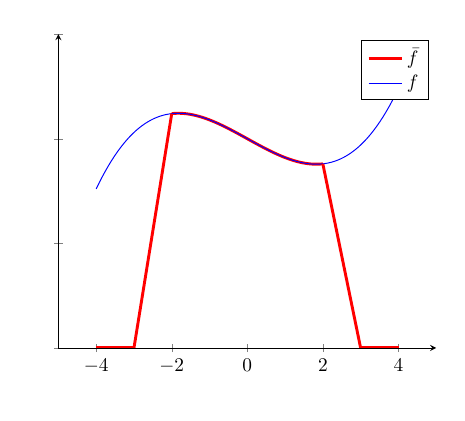
\begin{tikzpicture}[scale=0.7]
\begin{axis}[
    axis lines = left,
    xmin=-5,
    xmax=5,
    ymin=0,
    ymax=30,
    xlabel = $$,
    ylabel = {$$},
    yticklabels={,,}
]
%Below the red parabola is defined
\addplot [
    domain=-2:2, 
    samples=100, 
    line width=1.5,
    color=red,
]
{0.2*x^3 - 2*x + 20};
%Here the blue parabloa is defined
\addplot [
    domain=-4:4, 
    samples=100,         line width=0.5, 
    color=blue,
    ]
    {0.2*x^3 - 2*x + 20};
        \addlegendentry{$\bar f$}

\addplot [
    domain=3:4, 
    samples=100,
        line width=1.5, 
    color=red,
    ]
    {0};
\addplot [
    domain=-3:-2, 
    samples=100, 
    color=red,
       line width=1.5,
    ]
    {22.4*x+67.2};
    \addlegendentry{$f$}

\addplot [
    domain=-4:-3, 
    samples=100,
        line width=1.5, 
    color=red,
    ]
    {0};
    \addplot [
    domain=2:3, 
    samples=100, 
    color=red,
       line width=1.5,
    ]
    {-17.6*x+52.8};

\end{axis}
\end{tikzpicture}
		\end{center}
			  In Worten: $\bar f$ ist gleich $f$ in $[-k,k]$, null au\ss erhalb von $[-k-1,k+1]$ und verbindet dazwischen linear $0$ und $f(k)$ bzw. $f(-k)$. Die wichtige dazu gewonnene Information ist, dass $\bar f$ gleichm\"a\ss ig stetig ist. Das gilt, weil stetige Funktionen auf kompakten Mengen gleichm\"a\ss ig stetig sind (siehe Analysis 1). Jetzt kommt ein mehrfach genutzter Trick aus der Analysis. Wir addieren zwei Mal $0$ und nutzen die Dreicksungleichung
			 \begin{align}\label{F4}
				 \quad |\E[f(X_n)] - \E[f(X)]|
			 	\overset{\triangle}{\leq} \underbrace{\E[|f(X_n) - \bar f(X_n)|]}_{:= \text{ I}_n} + \underbrace{\E[|\bar f(X_n) - \bar f(X)|]}_{:= \text{ II}_n} + \underbrace{\E[|\bar f(X) - f(X)|]}_{:= \text{ III}_n}
			 \end{align}
			 und betrachten einzeln die Grenzwerte der drei Summanden. Aus (i), und weil $\bar f$ gleichmäßig stetig, wissen wir, dass $\text{II}_n \to 0$ f\"ur $n \to \infty$. F\"ur den dritten Summanden gilt
			 \begin{align*}
			 	\text{III}_n &= \E[|f(X) - \bar f(X)| \cdot (\mathbf 1_{[-k,k]}(X)+\mathbf{1}_{[-k,k]^C}(X))] \\
				&\leq 0+\E[2||f||_{\infty} \mathbf{1}_{[-k,k]^C}(X)]\\
			 	&= 2||f||_{\infty} \mathbb{P}(X \in [-k,k]^C)\\
				&= 2||f||_{\infty} \mathbb{P}(X \notin [-k,k])\\
				\overset{\text{Mon.}}&{\leq} 2||f||_{\infty} \mathbb{P}(X \notin [-k+1,k-1])
				< 2 || f ||_\infty \varepsilon,
			 \end{align*}
			 wegen der Wahl von $k$ und weil $f(x)-\bar f(x)=0$ f\"ur $x\in [-k,k]$. Schlie\ss lich noch der erste Summand. Wegen der angenommenen stochastischen Konvergenz gilt 
			 $$0\leq \mathbb P(X_n\notin [-k,k], X\in [-k+1,k-1])\leq \mathbb P(|X_n-X|>1)\rightarrow 0,\quad n\to\infty.$$ Damit zerlegen wir wie folgt:
			 \begin{align*}
			 	\quad \text{I}_n 
				&= \E[|f(X_n) - \bar f(X_n)|\cdot (\mathbf{1}_{[-k,k]}(X_n)+\mathbf{1}_{[-k,k]^C}(X_n)]\\
				&\leq 0+ \E[ 2||f||_\infty \mathbf 1_{[-k,k]^C}(X_n)]\\
				&=2|| f|| _\infty \mathbb P(X_n \notin [-k,k])\\
				&=2||f||_\infty \big( \mathbb P(X_n\notin [-k,k], X\in [-k+1,k-1])+\mathbb P(X_n\notin [-k,k],X\notin  [-k+1,k-1]) \big)\\
				&\leq 2||f||_\infty \big( \mathbb P(|X_n-X|\geq 1)+\mathbb P(X\notin [-k+1,k-1]) \big)\\
				&\leq 2||f||_\infty \big( \mathbb P(|X_n-X|\geq 1)+\varepsilon) \big).
			 \end{align*}
			Die rechte Seite konvergiert dann gegen $2||f||_\infty \varepsilon$. In der Rechnung haben wir viele kleine Eigenschaften benutzt, checkt es mal selber Zeile f\"ur Zeile: Monotonie und Linearit\"at von Erwartungswerten, dass Erwartungswerte von Indikatoren Wahrscheinlichkeiten sind (siehe Proposition \ref{rechenregeln}), sowie die $\sigma$-Additivit\"at und Monotonie von Ma\ss en. \smallskip			 
			 
			 Die drei einzelnen Betrachtungen zusammen ergeben wegen \eqref{F4}
			 
			  \[0\leq \limsup\limits_{n \to \infty} |\E[f(X_n)] - \E[f(X)]| \leq 2 ||f||_{\infty} \varepsilon + 0 + 2||f||_{\infty}\varepsilon. \] 
			 Weil $\varepsilon$ beliebig war, folgt daraus $\limsup\limits_{n \to \infty} |\E[f(X_n)] - \E[f(X)]|=0$ und damit $ \lim\limits_{n \to \infty} \E[f(X_n)] = \E[f(X)]$. Das ist die Konvergenz in Verteilung. \smallskip
			 
Die Hauptrichtungen sind nun vollst\"andig bewiesen. Wir zeigen jetzt noch, dass eine Umkehrung gilt, wenn der Grenzwert eine konstante Zufallsvariable ist:\smallskip

\textbf{Konvergenz in Verteilung gegen eine \underline{konstante} Zufallsvariable} $\Rightarrow$ \textbf{ Stochastische Konvergenz}:

Sei nun $(X_n)$ eine Folge von Zufallsvariablen, die gegen eine fast sicher konstante Zufallsvariable $X$ in Verteilung konvergiert. Sei $\eta\in\R$ der Wert, den $X$ $\mathbb P$-fast sicher annimmt und sei $\varepsilon>0$ beliebig. Sei nun $I=[\eta-\varepsilon, \eta+\varepsilon]$ und $f$ eine stetige Funktion mit $f\leq \mathbf 1_I$ sowie $f(\eta)=1$. Nat\"urlich gibt es so ein $f$, zum Beispiel das aus folgendem Bildchen:
\begin{center}



\tikzset{every picture/.style={line width=0.75pt}} %set default line width to 0.75pt        

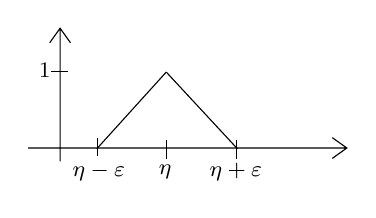
\begin{tikzpicture}[x=0.75pt,y=0.75pt,yscale=-1,xscale=1]
%uncomment if require: \path (0,300); %set diagram left start at 0, and has height of 300

%Shape: Axis 2D [id:dp6803750341520275] 
\draw  (266,150.59) -- (419.5,150.59)(281.35,92.88) -- (281.35,157) (412.5,145.59) -- (419.5,150.59) -- (412.5,155.59) (276.35,99.88) -- (281.35,92.88) -- (286.35,99.88)  ;
%Straight Lines [id:da7239111188912024] 
\draw    (332.5,114) -- (299,151) ;


%Straight Lines [id:da11710965322449962] 
\draw    (332.5,114) -- (366.83,151) ;


%Straight Lines [id:da1606239616323779] 
\draw    (284.95,113.75) -- (276.95,113.75) ;


%Straight Lines [id:da9124228840014664] 
\draw    (332.5,146.67) -- (332.5,155.67) ;


%Straight Lines [id:da9843095899175679] 
\draw    (366.5,146.67) -- (366.5,155.67) ;


%Straight Lines [id:da8761311329641914] 
\draw    (299.5,145.67) -- (299.5,154.67) ;



% Text Node
\draw (274,113) node  [font=\footnotesize] [align=left] {{\footnotesize 1}};
% Text Node
\draw (332,162) node   [align=left] {{\footnotesize $\eta$}};
% Text Node
\draw (366,162) node   [align=left] {{\footnotesize $\eta+\varepsilon$}};
% Text Node
\draw (300,162) node   [align=left] {{\footnotesize $\eta-\varepsilon$}};


\end{tikzpicture}
\end{center}
Wegen der angenommenen Konvergenz in Verteilung gilt damit
\begin{align*}
	1&=f(\eta)\\
	\overset{\ref{rechenregeln} \text{ (iii)}}&{=}\E[f(X)]\\
	&=\lim_{n\to\infty}\E[f(X_n)]\\
	\overset{\text{Monotonie}}&{\leq} \limsup_{n\to\infty} \E[\mathbf 1_{I}(X_n)]\\
	\overset{\ref{rechenregeln}\text{ (iv)}}&{=}\limsup_{n\to\infty} \mathbb P(X_n\in I)\leq 1,
\end{align*}
weil Wahrscheinlichkeiten immer durch $1$ dominiert sind. Weil obere und untere Schranke gleich sind, bekommen wir $\lim_{n\to\infty} \mathbb P(X_n\in I)=1$ und damit
\begin{align*}
	\mathbb P(|X_n-X|>\varepsilon)=\mathbb P(|X_n-\eta|>\varepsilon)=\mathbb P(X_n\notin I)=1-\mathbb P(X_n\in I)\to 0,\quad n\to\infty.
\end{align*}		
Warum tauchte gerade der Limes superior auf? Das liegt einfach nur daran, dass wir nicht wissen, ob der Grenzwert der Erwartungswerte existiert. Wir wissen das zwar f\"ur stetige Funktionen, aber der Indikator ist nicht stetig. \smallskip

\textbf{Stochastische Konvergenz } $\Rightarrow$ \textbf{ Fast sichere Konvergenz einer Teilfolge}:

Den Teil liefern wir nach dem Borel-Cantelli Lemma nach, siehe die Bemerkung \ref{bem4}.
%
%Wie immer gilt, dass man den Beweis genau anschauen sollte, wenn die Aussage nicht ganz klar ist. Wir nehmen an, dass die Folge $(X_n)$ stochastisch gegen $X$ konvergiert, f\"ur jedes $\varepsilon>0$ die Folge $a_n:=\mathbb P(|X_n-X|>\varepsilon)$ also eine Nullfolge ist. Wenn wir das mit Quantoren sauber ausschreiben, steht da also
%\begin{align}\label{sa}
%	\forall \varepsilon, \varepsilon'>0 \,\exists N\in \N: \mathbb P(|X_n-X|>\varepsilon)<\varepsilon', \quad \forall n\geq N.
%\end{align}
%Weil wir $\varepsilon$ und $\varepsilon'$ beliebig w\"ahlen d\"urfen, w\"ahlen wir $\varepsilon=\frac 1 k$ und $\varepsilon'=\frac{1}{2^k}$ f\"ur $k\in\N$. Wenn wir das zugeh\"orige $N$ aus \eqref{sa} als $n_k$ bezeichnen, so haben wir eine Teilfolge $X_{n_1}, X_{n_2}, ...$ gefunden, die folgendes Absch\"atzung erf\"ullt:
%\begin{align*}	
%	\mathbb P\Big(|X_{n_k}-X|>\frac 1 k\Big)<\frac{1}{2^k},\quad k\in\N.
%\end{align*}
%Um die fast sichere Konvergenz gerade dieser Teilfolge $X_{n_1}, X_{n_2}, ...$ gegen $X$ zu zeigen, nutzen wir folgende Beobachtung. Es gilt nat\"urlich
%\begin{align*}
%	\bigcap_{k=j}^\infty \Big\{\omega\in \Omega: |X_{n_k}(\omega)-X(\omega)|\leq\frac{1}{k} \Big\}\subseteq \big\{\omega\in \Omega: X_{n_k}(\omega) \to X(\omega)\big\}
%\end{align*}
%f\"ur alle $j\in\N$ oder alternativ, durch Komplementbildung und de Morgan, 
%\begin{align*}
%	\big\{\omega\in \Omega: X_{n_k}(\omega) \not\to X(\omega) \big\} \subseteq \bigcup_{k=j}^\infty \Big\{\omega\in \Omega: |X_{n_k}(\omega)-X(\omega)|>\frac{1}{k} \Big\}.
%\end{align*}
%Damit sind wir fertig: F\"ur $j\in\N$ beliebig gilt somit
%\begin{align*}
%	0&\leq \mathbb P(X_{n_k}\not \to X)\\
%	\overset{\text{Monotonie}}&{\leq}\mathbb P\Big(\bigcup_{k=j}^\infty\Big\{|X_{n_k}-X|>\frac{1}{k}\Big\}\Big)\\
%	\overset{\text{Subadd.}}&{\leq} \sum_{k=j}^\infty \mathbb P\Big(|X_{n_k}-X|>\frac 1 k \Big)\\
%	\overset{\text{Wahl der }n_k}&{\leq} \sum_{k=j}^\infty \frac{1}{2^k}.
%\end{align*}
%Weil $j$ beliebig war, k\"onnen wir auf der rechten Seite $j$ nach $+\infty$ schicken und damit gilt (die geometrische Reihe mit $q=\frac 1 2$ konvergiert) $0\leq \mathbb P(X_{n_k}\not \to X)\leq 0$ oder $\mathbb P(X_{n_k} \to X)=1$. Also konvergiert die Teilfolge $X_{n_1}, X_{n_2}, ...$ fast sicher gegen $X$.
\end{proof}

Aus dem Konvergenzdiagramm folgt nat\"urlich, dass fast sichere Konvergenz auch Konvergenz in Verteilung impliziert. \"Uberlegt doch mal, warum diese Aussage sehr viel schneller auch ohne den Umweg \"uber die stochastische Konvergenz folgt (Stichwort dominierte Konvergenz).\smallskip




	Das Ziel ist immer, die \enquote{starken} Konvergenzen (links im Bildchen) zu zeigen. Das geht leider nicht immer! Um die Begriffe mit Leben zu f\"ullen, zeigen wir drei ber\"uhmte S\"atze, je einen f\"ur stochastische Konvergenz, fast sichere Konvergenz und Konvergenz in Verteilung:
\begin{itemize}
	\item schwaches Gesetz der gro\ss en Zahlen (stochastische Konvergenz)
	\item starkes Gesetz der gro\ss en Zahlen (fast sichere Konvergenz)
	\item Zentraler Grenzwertsatz (Konvergenz in Verteilung)
\end{itemize}
Beim schwachen Gesetz der gro\ss en Zahlen werden wir merken, dass Konvergenz in $\mathcal L^p$ gerade f\"ur $p=1$ oder $p=2$ ein extrem n\"utzliches Werkzeug ist. Der Grund ist, dass man mit Momenten gut rumrechnen kann (Ausmultiplizieren, Linearit\"at, ...). Folgendes Resultat ist nicht sehr kompliziert, kann aber schon n\"utzlich sein. Sehr viel n\"utzlicher wird n\"achste Woche aber das starke Gesetzt der gro\ss en Zahlen sein!

\begin{satz}\label{schwaches}
\link{https://www.youtube.com/watch?v=e-i3vo2epBI&list=PLy5qRKPWp6SBwfc1kn-b66cWc84cOgvqZ&index=26&t=6815s} \textbf{[Schwaches Gesetz der großen Zahlen]}
	\begin{enumerate}[label=(\roman*)]
		\item Klassische Variante: Sind $X_1,X_2,...$ u.i.v. mit $\E[X_1^2] < \infty$, so gilt
		\[ \frac{1}{n} \sum_{k=1}^{n} X_k \overset{P}{\longrightarrow} \E[X_1], \quad n \to \infty. \]
		\item Variante mit schw\"acheren Annahmen: Sind $X_1,X_2,...$ quadratintegrierbar, paarweise unkorreliert (z. B. paarweise unabh\"angig) mit identischen Erwartungswert und
		\begin{align}
		 \frac{1}{n^2} \sum\limits_{k=1}^{n} \V(X_k) \to 0,\quad n\to\infty, \label{F1}
		\end{align}
		so gilt
		\[ \frac{1}{n} \sum_{k=1}^{n} X_k \overset{P}{\longrightarrow} \E[X_1], \quad n \to \infty. \]
	\end{enumerate}
\end{satz}
F\"urs bessere Verst\"andniss kann man \"uberlegen, wie die Annahme \enquote{identischer Erwartunswert} in (ii) ersetzt werden kann, da gibt es verschiedene M\"oglichkeiten. 
\begin{proof}
	(i)  Wenn man den Beweis gesehen hat, ist alles ziemlich simple: \textbf{Erst Tschebycheff, dann Bienaym\'e}. Mit Tschebycheff und Bienaym\'e gilt f\"ur beliebiges $\varepsilon>0$ aufgrund der u.i.v. Annahme
	\begin{align*}
		\mathbb{P}\Big(\Big|\frac{1}{n} \sum\limits_{k=1}^{n} X_k-\E[X_1]\Big| \geq \varepsilon\Big)
		&=\mathbb{P}\Big(\Big| \sum\limits_{k=1}^{n} X_k-n\E[X_1)\Big| \geq n \varepsilon\Big)\\
		\overset{\ref{Markov}}&{\leq} \frac{\V \big[\sum_{k=1}^n X_k\big] }{n^2\varepsilon^2}\\
		\overset{\ref{bien}}&{=} \frac{\sum\limits_{k=1}^{n} \V[X_k]}{n^2 \varepsilon^2}\\
		& = \frac{n \cdot \V[X_1]}{n^2 \varepsilon^2} \to 0, \quad n \to \infty.
		\end{align*}
		Also gilt $\frac{1}{n}\sum_{k=1}^n X_k\overset{P}{\rightarrow} \E[X_1]$ f\"ur $n\to\infty$. Beachtet dabei, dass wir f\"ur Tschebycheff $\E[\sum_{k=1}^n X_k]=n\E[X_1]$ genutzt haben. Um ganz genau zu sein (und wir wollen nat\"urlich genau sein!), merken wir noch an, dass \enquote{$>$} oder \enquote{$\geq$} in der Definition der schwachen Konvergenz nat\"urlich keine Rolle spielt, $\varepsilon$ ist schlie\ss lich beliebig.\smallskip
		
		Man kann das Argument auch anders hinschreiben. Benutzt zum \"Uben doch mal statt Tschebycheff die Markov Ungleichung mit $h(x)=x^2$ plus die Verschiebungsformel f\"ur die Varianz.\smallskip
				
		(ii) Um die schw\"acheren Annahmen von (ii) zu verstehen, brauchen wir nur in den vier Zeilen des Arguments zu schauen, wie wir die Unabh\"angigkeit abschw\"achen k\"onnen, so dass die Konvergenz immer noch folgt. Wir sehen dann sofort, dass f\"ur Bienaym\'e nur paarweise unkorreliert gebraucht wird, dann aber f\"ur die Konvergenz noch \eqref{F1} gefordert werden muss (es wird nicht mehr identisch verteilt angenommen, es gilt also nicht $\V[X_k]=\V[X_1]$). Schaut euch das in Ruhe an, um die Idee \enquote{erst Tschebyscheff, dann Bienaym\'e} einzubrennen.
\end{proof}

	Zum besseren Verst\"andnis kann man mal ausprobieren, ob man das schwache Gesetz genauso mit der Annahme $\E[|X_1|]<\infty$ beweisen k\"onnte. Warum funktioniert der Beweis nicht, wenn man die Markovungleichung f\"ur das erste Moment statt f\"ur das zweite Moment ausprobiert? Der Trick an dem Beweis mit zweiten Momenten ist, dass die Varianz der Summe, die eigentlich aus $n^2$ vielen Summanden besteht, sich aufgrund der Annahme (unabh\"angig oder unkorreliert) zu einer Summe aus nur $n$ vielen Summanden reduziert (im Beweis von Bienaym\'e k\"urzen sich die meisten Terme raus). Damit dominiert der Nenner mit $n^2$ und die obere Schranke konvergiert gegen $0$. Der Effekt passiert beim ersten Moment nicht, weil keine \enquote{gemischten Terme} $\E[X_iX_j]=0$ auftauchen. Deshalb st\"unde sowohl in Z\"ahler als auch in Nenner etwas mit $n$, die obere Schranke w\"urde also nicht gegen $0$ konvergieren, in Formeln (f\"ur $\E[X_1]=0$):
	\begin{align*}
		\mathbb{P}\Big(\Big|\frac{1}{n} \sum\limits_{k=1}^{n} X_k\Big| \geq \varepsilon\Big)
		&\overset{\ref{Markov},\, h(x)=|x|}{\leq} \frac{\E \big[\big|\sum_{k=1}^n X_k\big|\big] }{n\varepsilon}\leq \frac{\sum_{k=1}^n \E[|X_k|]}{n\varepsilon}= \frac{n\E[|X_1|]}{n\varepsilon} \not\to 0,
	\end{align*}
	f\"ur $n\to\infty$. Genau den selben Effekt werden wir beim Beweis des starken Gesetzes der gro\ss en Zahlen sehen, bei dem wir endliche 4.te Momente annehmen und bei der Markovungleichung mit $h(x)=x^4$ genug Summanden verschwinden, dass der Nenner dominiert.
	
	
%\begin{bem}
%	Gilt $\E[X_2] < \infty$, so gilt $\V(X) = \V(X+a)$. Warum? $\V(X+a) = \E[(X+a -\E[X+a])^2] = \E[(X+a -(\E[X]+\E[a]))^2] = \E[(X -\E[X])^2] = \V(X)$.
%\end{bem}

%\begin{proof}
%	\OE \space gelte $\E[X_1] = 0$. Warum? Wenn nicht, betrachte $Y_n = X_n - \E[X_n]$ (das nennt man zentrieren). Damit gilt 
%	\begin{gather*}
%		\mathbb{P}\Big(\Big|\frac{1}{n} \sum\limits_{i=1}^{n} (X_i - \E[X_1]) - 0\Big| > \varepsilon\Big) = \mathbb{P}\Big(\Big|\frac{1}{n} \sum\limits_{i=1}^{n} (X_i - \E[X_i]) - 0\Big| > \varepsilon\Big) \\
%		= \mathbb{P}\Big(\Big|\frac{1}{n} \sum\limits_{i=1}^{n} Y_i - 0\Big| > \varepsilon\Big) \to 0, \: n \to \infty,
%	\end{gather*}
%	weil $\E[Y_i] = \E[X_i - \E[X_i]] = \E[X_i] - \E[X_i] = 0$.
%	Sei also $\E[X_1] = 0$. 
%	\begin{gather*}
%		\mathbb{P}\Big(\Big|\frac{1}{n} \sum\limits_{i=1}^{n} X_i - 0\Big| > \varepsilon\Big) = \mathbb{P}\Big(\Big|\frac{1}{n} \sum\limits_{i=1}^{n} X_i - \E[\frac{1}{n} \sum\limits_{i=1}^{n} X_i]\Big| > \varepsilon\Big) \\
%		\overset{\text{\ref{tscheby}}}{\leq} \frac{\V\Big(\frac{1}{n} \sum\limits_{i=1}^{n} X_i\Big)}{\varepsilon^2} = \frac{\frac{1}{n^2} \V\Big(\sum\limits_{i=1}^{n} X_i\Big)}{\varepsilon^2} \overset{\text{\ref{bien}}}{=} \frac{\frac{1}{n^2} \sum\limits_{i=1}^{n} \V\Big(X_i\Big)}{\varepsilon^2}  \\
%		= \frac{\frac{1}{n^2} \cdot n \cdot \sum\limits_{i=1}^{n} \V\Big(X_i\Big)}{\varepsilon^2} = \frac{\sum\limits_{i=1}^{n} \V\Big(X_i\Big)}{n \varepsilon^2} \to 0, \: n \to \infty.
%	\end{gather*}
%\end{proof}


\section{Starkes Gesetz der großen Zahlen} \marginpar{\textcolor{red}{Vorlesung 26}}
	Was bedeutet die stochastische Konvergenz, bzw. warum ist sie schwach? Seien als Beispiel $X_1,X_2,...$ u.i.v. Würfel, also diskret gleichverteilt auf $\{1,...,6\}$. Wegen $\E[X_1]=3,5$ bedeutet das schwache Gesetz der großen Zahlen (w\"ahle zum Beispiel $\varepsilon=0.01$), dass 
	\[ \mathbb{P}\Big(3,49 < \frac{1}{n} \sum\limits_{i=1}^{n} X_i < 3,51\Big) = \mathbb{P}\Big(\Big|\frac 1 n\sum\limits_{i=1}^{n} X_i - \E[X_1]\Big| < 0,01\Big) \to 1, \quad n \to \infty. \]
	In Worten steht hier: \enquote{Der Mittelwert wird mit hoher Wahrscheinlichkeit nah bei 3,5 liegen, wenn $n$ groß ist.} Es wird damit nicht ausgeschlossen, dass der Mittelwert mit kleiner Wahrscheinlichkeit weit vom Erwartungswert entfernt liegt. Genau hier liegt der Unterschied zum starken Gesetz der gro\ss en Zahlen, das wir als n\"achstes beweisen wollen. Hier wird die stochastische Konvergenz durch fast sichere Konvergenz ersetzt. Weil in der Definition der fast sicheren Konvergenz alle $n$ gemeinsam \textit{innerhalb} der Wahrscheinlichkeit auftauchen, $\mathbb P(X_n\to X)=1$, kann der Effekt nicht auftreten.\smallskip

	
Als Hilfsmittel f\"ur den Beweis diskutieren wir zun\"achst das Borel-Cantelli Lemma. Dazu zun\"achst ein paar Definitionen:	
\begin{deff}
\link{https://www.youtube.com/watch?v=AfWbQxemkRI&list=PLy5qRKPWp6SBwfc1kn-b66cWc84cOgvqZ&index=27&t=235s}
	Sei $(\Omega, \cA, \mathbb{P})$ ein Wahrscheinlichkeitsraum und seien $A_1,A_2,... \in \cA$ beliebige Ereignisse.
	\begin{enumerate}[label=(\roman*)]
		\item \begin{align*}
			\limsup\limits_{n \to \infty} A_n 
			&:= \bigcap_{n=1}^{\infty} \bigcup_{k=n}^{\infty} A_k\\
			&= \{ \omega \in \Omega\colon \omega \in A_n \text{ für unendlich viele } n \}\\ 
			\overset{\text{Notation}}&{=} \{ A_n \text{ unendlich oft} \} 
		\end{align*}
		heißt \textbf{Limes superior} der Folge $(A_n)$ von Ereignissen.
		\item \begin{align*}
			\liminf\limits_{n \to \infty} A_n 
			&:= \bigcup_{n=1}^{\infty} \bigcap_{k=n}^{\infty} A_k\\
			&= \{ \omega \in \Omega\colon \omega \in A_n \text{ schließlich immer} \}\\
			\overset{\text{Notation}}&{=} \{ A_n \text{ schließlich immer} \}
		\end{align*}
		\textbf{Limes inferior} der Folge $(A_n)$ von Ereignissen.
	\end{enumerate}
\end{deff}
Weil aufgrund der Definition einer $\sigma$-Algebra abz\"ahlbare Schnitte und Vereinigungen wieder in $\mathcal A$ sind, sind auch $\limsup_{n\to\infty} A_n$ und $\liminf_{n\to\infty} A_n$ in $\mathcal A$. Wem der Begriff \enquote{schlie\ss lich immer} suspekt ist, der oder die schaue einfach die formelle Definition an. Diese besagt, dass es eine nat\"urliche Zahl $n$ gibt, so dass das Ereigniss danach \textit{immer} eintritt (der Durchschnitt von Mengen enth\"alt alle Elemente, die in allen Mengen enthalten sind).\smallskip

Tats\"achlich haben die neuen Begriffe $\liminf$ und $\limsup$ f\"ur Mengen auch etwas mit den uns bekannten Begriffen $\liminf$ und $\limsup$ f\"ur Folgen zu tun:
\begin{lemma}
\link{https://www.youtube.com/watch?v=AfWbQxemkRI&list=PLy5qRKPWp6SBwfc1kn-b66cWc84cOgvqZ&index=27&t=579s}
	Sei $(\Omega, \cA, \mathbb{P})$ ein Wahrscheinlichkeitsraum und seien $A_1,A_2,... \in \cA$ beliebige Ereignisse. Dann gelten:
	\begin{enumerate}[label=(\roman*)]
		\item $ \liminf\limits_{n \to \infty} A_n \subseteq \limsup\limits_{n \to \infty} A_n,$
		\item $(\liminf\limits_{n \to \infty} A_n)^C = \limsup\limits_{n \to \infty} A_n^C,$
		\item $\limsup\limits_{n \to \infty} \mathbf{1}_{A_n}(\omega) = \mathbf{1}_{\limsup\limits_{n \to \infty} A_n}(\omega),\quad \forall \omega \in \Omega,$
		\item $\liminf\limits_{n \to \infty} \mathbf{1}_{A_n}(\omega) = \mathbf{1}_{\liminf\limits_{n \to \infty} A_n}(\omega),\quad \forall \omega \in \Omega.$
	\end{enumerate}
\end{lemma}

\begin{proof}
	Denkt einfach mal kurz dar\"uber nach, was $\liminf_{n\to\infty} a_n=1$ oder $\liminf_{n\to\infty} a_n=0$ f\"ur eine reelle Folge $(a_n)$ bedeutet, wenn diese nur die Werte $0$ und $1$ annimmt. \"Ubung.
\end{proof}

Das Borel-Cantelli Lemma gibt uns gleich ein Kriterium, ob die Wahrscheinlichkkeit des $\limsup A_n$ null ist oder (mit einer st\"arkeren Annahme) $1$ ist. Daf\"ur basteln wir mit Zufallsvariablen rum, alles basiert auf folgender Bemerkung:
\begin{bem}\label{ereig}
\link{https://www.youtube.com/watch?v=AfWbQxemkRI&list=PLy5qRKPWp6SBwfc1kn-b66cWc84cOgvqZ&index=27&t=915s}
	Sei $(\Omega, \cA, \mathbb{P})$ ein Wahrscheinlichkeitsraum und seien $A_1,A_2,... \in \cA$ beliebige Ereignisse. Dann gilt
	\begin{align*}
		A_1, A_2, ... \text{ sind unabh\"angig}\quad \Leftrightarrow\quad  \mathbf{1}_{A_1},\mathbf{1}_{A_2},... \text{ sind unabhängig},
	\end{align*}	
	wobei wir auch die Unabh\"angigkeit durch paarweise Unabh\"angigkeit ersetzten k\"onnen.
	Beachte: $A_1, A_2, ...$ ist ein Folge von Ereignissen, wohingegen $\mathbf{1}_{A_1},\mathbf{1}_{A_2},... $ eine Folge von Zufallsvariablen ist. Das ist also ein guter Moment, in Kapitel \ref{Sunab} die Definitionen von Unabh\"angigkeit von Ereignissen und Zufallsvariablen nochmal zu vergleichen! Warum gilt die \"Aquivalenz? Checken wir die Definitionen:
	\begin{align*}
		\mathbf{1}_{A_1},\mathbf{1}_{A_2},... \text{ unabh\"angig}\quad 
		\overset{\text{Def. }\ref{unab}}&{\Leftrightarrow} \quad \sigma(\mathbf{1}_{A_1}),\sigma(\mathbf{1}_{A_2}),... \text{ unabhängig}\\
		\overset{\ref{yu}}&{\Leftrightarrow}\quad \{ \emptyset, \Omega, A_1, A_1^C \},\{ \emptyset, \Omega, A_2, A_2^C \}, ... \text{ unabhängig}\\
		&\Leftrightarrow\quad A_1, A_2, ... \text{ unabh\"angig}.
	\end{align*}
F\"ur die dritte \"Aquivalenz haben wir Definition \ref{Ka} genutzt, sowie die Eigenschaft, dass Unabh\"angigkeit von Ereignissen sich auch auf die Komplemente \"ubertr\"agt (\"Ubung). 
	
	
\end{bem}

\begin{satz}\label{BC}
\link{https://www.youtube.com/watch?v=AfWbQxemkRI&list=PLy5qRKPWp6SBwfc1kn-b66cWc84cOgvqZ&index=27&t=1127s} \textbf{[Borel-Cantelli-Lemma]}
	Sei $(\Omega, \cA, \mathbb{P})$ ein Wahrscheinlichkeitsraum und seien $A_1,A_2,... \in \cA$ beliebige Ereignisse, so gelten:
	\begin{enumerate}[label=(\roman*)]
		\item \[ \sum\limits_{n = 1}^{\infty} \mathbb{P}(A_n) < \infty \quad \Rightarrow\quad  \mathbb{P}\big(\limsup\limits_{n \to \infty} A_n\big) =0. \]
		\item Sind die $A_1, A_2, ...$ \textit{zusätzlich} paarweise unabhängig, so gilt \[ \sum\limits_{n = 1}^{\infty} \mathbb{P}(A_n) = \infty \quad \Rightarrow \quad \mathbb{P}\big(\limsup\limits_{n \to \infty} A_n\big) = 1. \]
	\end{enumerate}
\end{satz}
	Damit kennt ihr nun euer erstes \enquote{0-1-Gesetz}: Sind die Ereignisse $A_1, A_2, ...$ paarweise unabh\"angig, so gilt automatisch $\mathbb P(\limsup_{n\to\infty} A_n)\in \{0,1\}$ und
	\begin{align*}
		\mathbb P(\limsup_{n\to\infty}A_n)=1\quad \Longleftrightarrow \quad\mathbb P(\limsup_{n\to\infty}A_n)>0\quad \Longleftrightarrow \quad  \sum_{n=1}^\infty \mathbb P(A_n)=\infty.
	\end{align*}
	 Das n\"utzliche an 0-1-Gesetzen ist, dass man nur zeigen muss, dass etwas strikt positive Wahrscheinlichkeit hat, um sogar Wahrscheinlichkeit $1$ zu schlie\ss en. 

\begin{proof}\abs
	\begin{enumerate}[label=(\roman*)]
		\item \enquote{triviale Rechnung}: Die einfache Richtung folgt aus einfachen Manipulationen mit Mengen und Eigenschaften von Ma\ss en:
		\begin{align*}
			\mathbb{P}(\limsup\limits_{n \to \infty} A_n) 
			&= \mathbb{P}\Big(\bigcap_{n=1}^{\infty} \bigcup_{k=n}^{\infty} A_k\Big)\\
			\overset{\text{Stet. Ma\ss e}}&{=}\lim\limits_{N \to \infty} \mathbb{P}\Big(\bigcap_{n=1}^{N} \bigcup_{k=n}^{\infty} A_k\Big)\\
			\overset{\text{Monotonie}}&{\leq}\lim\limits_{N \to \infty} \mathbb{P}\Big(\bigcup_{k=N}^{\infty} A_k\Big) \\
			\overset{\text{Subadd.}}&{\leq} \lim\limits_{N \to \infty} \sum\limits_{k=N}^{\infty} \mathbb{P}(A_k) = 0.
		\end{align*}
		Die letzte Gleichheit gilt nach Annahme und Analysis 1 (Eigenschaft konvergenter Reihen), weil $\sum_{k=1}^\infty \mathbb P(A_k)<\infty$ angenommen wurde.
		\item Die R\"uckrichtung ist deutlich schwieriger, wir nutzen die sogenannte \enquote{zweite-Momente-Methode}. Daf\"ur werden erstes und zweites Moment einer geeigneten Zufallsvariable miteinander verglichen. Wir betrachten im Folgenden die Zufallsvariablen $\mathbf 1_{A_n}$, die aufgrund von Bemerkung \ref{ereig} unabh\"angig sind. Weil die Zufallsvariablen nur die Werte $0$ und $1$ annehmen, sind sie Bernoulli-verteilt. Genauer, es gilt $\mathbf 1_{A_n}\sim \operatorname{Ber}(p_n)$, wobei $p_n=\mathbb P(A_n)$ die Wahrscheinlichkeit f\"ur den Wert $1$ ist. Kleine Erinnerung: F\"ur $\operatorname{Ber}(p)$-verteilte Zufallsvariablen ist der Erwartungswert $p$ und die Varianz $p(1-p)$. Das werden wir im Folgenden ausnutzen.\smallskip
		
		Wir betrachten die Folge
		\[ Z_k = \sum\limits_{n=1}^{k} \mathbf{1}_{A_n},\quad k\in\N, \]
		weil mit dieser Folge $\limsup_{n\to\infty} A_n$ beschrieben werden kann:
		\begin{align}\label{kyp}
			\omega \in \limsup\limits_{n \to \infty} A_n \quad \Leftrightarrow \quad +\infty=\sum\limits_{n=1}^{\infty} \mathbf{1}_{A_n}(\omega) = \lim\limits_{k \to \infty} Z_k(\omega).
		\end{align}
		Das gilt nat\"urlich weil die Reihe nur aus Summanden $0$ oder $1$ besteht und daher unendlich ist genau dann, wenn unendlich viele Summanden $1$ sind, also wenn $\omega$ in unendlich vielen $A_n$ ist. F\"ur Erwartungswert und Varianz gelten
		 \begin{align*}
		 	\E[Z_k] &= \sum\limits_{n=1}^{k} \E[\mathbf{1}_{A_n}] = \sum\limits_{n=1}^{k} \mathbb P(A_n) \overset{\text{Ann.}}{\longrightarrow}+\infty, \quad k \to \infty,
		\end{align*}
		sowie
		\begin{align*}
		 	\V[Z_k] \underset{\text{\ref{ereig}}}&{\overset{\text{\ref{bien}}}{=}} \sum\limits_{n=1}^{k}\V[\mathbf{1}_{A_n}]
		 	= \sum\limits_{n=1}^{k} \mathbb P(A_n)(1-\mathbb P(A_n)) \leq \sum\limits_{n=1}^{k} \mathbb P(A_n) = \E[Z_k],
		 \end{align*}
		 weil unabh\"angige Zufallsvariablen auch unkorrelliert sind. Jetzt benutzen wir Tschebyscheff mit den Formeln f\"ur Erwartungswert und Varianz:
		  \begin{align}\label{absch}
		 	\mathbb{P}\Big(|Z_k - \E[Z_k]| \geq \frac{\E[Z_k]}{2}\Big) \overset{\ref{Markov}}{\leq}\frac{\V[Z_k]}{\frac{1}{4} \E[Z_k]^2} \leq \frac{4\E[Z_k]}{\E[Z_k]^2} = \frac{4}{\E[Z_k]} \to 0,
		 \end{align}
		 f\"ur $k\to\infty$. Sei nun $\lambda > 0$ beliebig. Dann existiert wegen der Divergenz der Erwartungswerte gegen unendlich ein $k_0 \in \N$ mit $\frac{\lambda}{\E[Z_k]} < \frac{1}{2}$ f\"ur alle $k\geq k_0$.
		 Weil aufgrund der Definition von $Z_k$ auch $Z_k \leq \sum\limits_{n=1}^{\infty} \mathbf{1}_{A_n}$ gilt, bekommen wir für beliebiges $k \geq k_0$
		 \begin{align*}
		 	\mathbb{P}\Big(\sum\limits_{n=1}^{\infty} \mathbf{1}_{A_n} < \lambda \Big)& \leq \mathbb{P}(Z_k < \lambda)\\
			& = \mathbb{P}\Big(\frac{Z_k}{\E[Z_k]} < \frac{\lambda}{\E[Z_k]}\Big)\\
			& \leq \mathbb{P}\Big(\frac{Z_k}{\E[Z_k]} < \frac{1}{2}\Big)\\ 
		 	&= \mathbb{P}\Big(\frac{Z_k}{\E[Z_k]} - 1 < -\frac{1}{2}\Big)\\
			& \leq \mathbb{P}\Big(\Big|\frac{Z_k}{\E[Z_k]} - 1\Big| \geq \frac{1}{2}\Big)\\
		 	\overset{\text{Vor.}}&{=} \mathbb{P}\Big(\big|Z_k - \E[Z_k]\big| \geq \frac{\E[Z_k]}{2}\Big) \overset{\text{\eqref{absch}}}{\longrightarrow} 0, \quad k \to \infty.
		 \end{align*}
		Also gilt $\mathbb{P}\big(\sum\limits_{n=1}^{\infty} \mathbf{1}_{A_n} < \lambda \big)=0$. Weil $\lambda$ beliebig gew\"ahlt war, folgt aufgrund der Stetigkeit von Ma\ss en auch $\mathbb{P}\big(\sum\limits_{n=1}^{\infty} \mathbf{1}_{A_n} < \infty \big)=\lim_{N\to\infty}\mathbb{P}\big(\sum\limits_{n=1}^{\infty} \mathbf{1}_{A_n} < N \big) =0$. Wegen \eqref{kyp} gilt nun \[ \mathbb{P}\big(\limsup\limits_{n \to \infty}A_n\big) = \mathbb{P}\Big(\sum\limits_{n=1}^{\infty} \mathbf{1}_{A_n} = +\infty\Big) = 1. \]
	\end{enumerate}
\end{proof}
Kleine Anmerkung an dieser Stelle: Wenn im zweiten Teil statt paarweiser Unabh\"angigkeit sogar Unabh\"angigkeit angenommen wird, dann gibt es einen einfacheren Beweis f\"ur Teil (ii):
\begin{align*}
	\mathbb P\big((\limsup\limits_{n \to \infty} A_n)^C\big)	\overset{\text{de Morgan}}&= \mathbb{P}\Big(\bigcup_{n=1}^{\infty} \bigcap_{k=n}^{\infty} A^C_k\Big)\\
	\overset{\text{Subadd.}}&\leq \sum_{n=1}^\infty \mathbb{P}\Big(\bigcap_{k=n}^{\infty} A^C_k\Big)\\
		\overset{\text{Stet. Ma\ss e}}&\leq \sum_{n=1}^\infty \lim_{N\to\infty} \mathbb{P}\Big(\bigcap_{k=n}^NA^C_k\Big)\\
		\overset{\text{Unab.}}&= \sum_{n=1}^\infty \lim_{N\to\infty} \prod_{k=n}^N (1-\mathbb{P}(A_n))\\
		\overset{1-x\leq e^{-x}}&\leq \sum_{n=1}^\infty \lim_{N\to\infty} \prod_{k=n}^N e^{-\mathbb{P}(A_n)}\\
		&= \sum_{n=1}^\infty \lim_{N\to\infty}  e^{-\sum_{k=n}^N\mathbb{P}(A_n)}
		\overset{\text{Vor.}}{=}\sum_{n=1}^\infty \,0=0.
\end{align*}
Checkt mal genau, warum dieser Beweis Unabh\"angigkeit statt nur paarweise Unabh\"angigkeit benutzt! Die komplizierte Variante wurde haupts\"achlich aus didaktischen Gr\"unden gew\"ahlt, um Argumente mit der Markovungleichung und Bernoulli-Zufallsvariablen zu wiederholen.\smallskip

Nach diesem sehr abstrakten Highlight, nun zur\"uck zur fast sicheren Konvergenz und dem starken Gesetz der gro\ss en Zahlen. 
\begin{korollar}\label{ko}
\link{https://www.youtube.com/watch?v=AfWbQxemkRI&list=PLy5qRKPWp6SBwfc1kn-b66cWc84cOgvqZ&index=27&t=3005s}
	Seien $X, X_1, X_2, ...$ Zufallsvariablen auf einem Wahrscheinlichkeitsraum $(\Omega, \mathcal A, \mathbb P)$, dann gelten:
	\begin{enumerate}[label=(\roman*)]
		\item $$\sum_{n=1}^\infty \mathbb P(|X_n-X|>\varepsilon)<\infty\text{  f\"ur alle }\varepsilon>0 \quad\Longrightarrow\quad X_n\overset{\text{f.s.}}{\to}X,\quad n\to\infty.$$
		\item Unter der zus\"atzlich Annahme $X_1-X, X_2-X, ...$ sind paarweise unabh\"angig, gilt: $$\sum_{n=1}^\infty \mathbb P(|X_n-X|>\varepsilon)=+\infty\text{ f\"ur ein }\varepsilon>0\quad \Longrightarrow\quad X_n\overset{\text{f.s.}}{\not\to}X, \quad n\to\infty.$$
	\end{enumerate}
\end{korollar}
\begin{proof}
	Beide Aussagen folgen sofort aus Borel-Cantelli:
\begin{enumerate}[label=(\roman*)]
\item Mit $\varepsilon=\frac 1 k$ impliziert das Borel-Cantelli-Lemma $\mathbb P(|X_n-X|>\frac 1 k\text{ unendlich oft})=0$ bzw. $\mathbb P(|X_n-X|>\frac 1 k\text{ nur endlich oft})=1$ f\"ur alle $k\in\N$. Daraus folgt
	\begin{align*}
		\mathbb P(X_n\to X)&=\mathbb P\Big(\Big\{\omega: \forall k \in \N\, \exists N\in \N: |X_n(\omega)-X(\omega)|\leq \frac{1}{k}\, \forall n\geq N\Big\}\Big)\\
		&=\mathbb P\Big(\bigcap_{k=1}^\infty \Big\{\omega:  \exists N\in \N: |X_n(\omega)-X(\omega)|\leq \frac{1}{k}\, \forall n\geq N\Big\}\Big)\\
		&=\mathbb P\Big(  \Big\{\omega: |X_n(\omega)-X(\omega)|>\frac{1}{k}\text{ endlich oft}\Big\}\Big)=1,
	\end{align*}
	weil der Durchschnitt abz\"ahlbar vieler Mengen von Ma\ss{} $1$ auch Ma\ss{} $1$ hat (wegen Komplementbildung, abz\"ahlbare Vereinigungen von Nullmengen sind Nullmengen). Denkt an dieser Stelle nochmal daran, dass wir manchmal in Wahrscheinlichkeiten die $\omega$ bei Zufallsvariablen weglassen weil es sich besser liest.	
\item Borel-Cantelli impliziert $\mathbb P(|X_n-X|>\varepsilon\text{ unendlich oft})=1$, also ist die Wahrscheinlichkeit, dass $X_n$ gegen $X$ konvergiert, sogar $0$.
\end{enumerate}
\end{proof}

Wegen Borel-Cantelli k\"onnen wir den Unterschied von stochastischer und fast sicherer Konvergenz nun besser verstehen:
\begin{bem}\label{bem4}
\link{https://www.youtube.com/watch?v=AfWbQxemkRI&list=PLy5qRKPWp6SBwfc1kn-b66cWc84cOgvqZ&index=27&t=3657s} \textbf{[Stochastische Konvergenz vs. fast sichere Konvergenz]}
\begin{itemize}
\item	Um stochastische Konvergenz zu zeigen, muss $a_n:=\mathbb P(|X_n-X|>\varepsilon)$ f\"ur beliebiges $\varepsilon>0$  eine Nullfolge sein. Konvergiert die Nullfolge so schnell gegen $0$, dass auch der Reihengrenzwert $\sum_{n=1}^\infty a_n$ endlich ist, so konvergiert nach Korollar \ref{ko} die Folge $(X_n)$ fast sicher gegen $X$. Wenn wir uns an Analysis 1 erinnern, ist es ein gro\ss er Unterschied, ob die Reihe \"uber eine Folge konvergiert oder die Folge eine Nullfolge ist. Beispielsweise reicht f\"ur stochastische Konvergenz die Absch\"atzung $\mathbb P(|X_n-X|>\varepsilon)\leq \frac{1}{n}$ f\"ur fast sichere Konvergenz nicht!
	\item Wir m\"ussen noch einen Teil des Beweises von Satz 4.5.11 nachliefern. Das folgt aus dem ersten Teil des Korollars mit der Wahl der Teilfolge $n_k$, die $$\mathbb P\Big(|X_{n_k}-X|>\frac 1 k\Big)<\frac{1}{2^k}$$ erf\"ullt.
\end{itemize}
\end{bem}




\begin{beispiel}
\link{https://www.youtube.com/watch?v=AfWbQxemkRI&list=PLy5qRKPWp6SBwfc1kn-b66cWc84cOgvqZ&index=27&t=4036s}
Schauen wir uns das Beispiel \ref{Adam} nochmal etwas allgemeiner an, um ein konkretes Beispiel f\"ur Korollar \ref{ko} zu haben: Seien $X_1, X_2, ... $ unabh\"angige Zufallsvariablen mit $$\mathbb{P}(X_n = 1) = \frac{1}{n^p}, \quad \mathbb{P}(X_n = 0) = 1 - \frac{1}{n^p},$$ also $X_n \sim \operatorname{Ber}(\frac{1}{n^p})$, $n \in \N$. Man stelle sich wieder unabh\"angige Versuche vor ($1$ bedeutet \enquote{Erfolg}, $0$ bedeutet \enquote{Misserfolg}), bei denen die Wahrscheinlichkeit f\"ur \enquote{Erfolg} immer kleiner wird. Fragen wir uns wieder: Konvergiert die Folge fast sicher gegen die Zufallsvariable $X=0$? Wegen der angenommenen Unabh\"angigkeit gilt mit Korollar \ref{ko} 
\begin{align*}
	X_n\overset{\text{f.s.}}{\to} 0,\quad n\to\infty \quad &\Leftrightarrow\quad \sum_{n=1}^\infty \mathbb P(X_n=1)=\sum_{n=1}^\infty \frac{1}{n^p}<+\infty\quad
	\Leftrightarrow\quad p>1.
\end{align*}
Ausformuliert ist die Aussage noch spektakul\"arer weil die Konvergenz gegen $0$ einer Folge mit Werten $0$ oder $1$ bedeutet, dass die Folge irgendwann nur noch den Wert $0$ annimmt. Ist $p\leq 1$, so ist der Versuch also immer mal wieder erfolgreich, wohingegen f\"ur $p>1$ der Versuch nur endlich oft erfolgreich ist. Wenn man bedenkt, dass der Versuch unendlich oft ausgef\"uhrt wird und jedes Mal positive Wahrscheinlichkeit f\"ur Erfolg besteht, ist der Fall $p>1$ schon \"uberraschend! Hier ist ein ganz konkretes Anwendungsbeispiel. Stellt euch vor, ihr schreibt jedes Jahr die Stochastik 1 Klausur, ohne euch mit dem Inhalt zu besch\"aftigen. Weil ihr den Inhalt mit der Zeit vergesst, wird die Wahrscheinlichkeit des Bestehens immer kleiner. Die Frage ist nun: Wenn ihr immer wieder probiert, werdet ihr irgendwann bestehen? Das Beispiel zeigt, dass das davon abh\"angt, wie schnell die Bestehenswahrscheinlichkeit f\"allt, oder anders formuliert, wie schnell ihr vergesst.
\end{beispiel}


%Hier kommt noch eine manchmal n\"utzliche Folgerung von Borel-Cantelli:
%\begin{korollar}
%	Seien $X, X_1, X_2, ...$ Zufallsvariablen auf einem Wahrscheinlichkeitsraum $(\Omega, \mathcal A, \mathbb P)$, die stochastisch gegen $X$ konvergieren. Dann gibt es eine Teilfolge $X_{n_1}, X_{n_2},...$, die sogar fast sicher gegen $X$ konvergiert.
%\end{korollar}
%\begin{proof}
%	Wegen der stochastischen Konvergenz ist $a_n:=\mathbb P(|X_n-X|>\frac 1 k)$ eine Nullfolge f\"ur alle $k\in\N$. Wir w\"ahlen die $n_k$ dann so, dass $a_{n_k}\leq \frac{1}{2^k}$ gilt. Also gilt $$\sum_{k=1}^\infty \mathbb P(|X_{n_k}-X|>\frac 1 k)\leq \sum_{k=1}^\infty \frac{1}{2^k}<\infty$$ und mit Korollar \ref{ko} folgt $X_{n_k}\overset{\text{f.s.}}{\to}X, k\to\infty$ 
%\end{proof}


Jetzt zum starken Gesetz der gro\ss en Zahlen:

\begin{satz}\label{sGGZ}
\link{https://www.youtube.com/watch?v=AfWbQxemkRI&list=PLy5qRKPWp6SBwfc1kn-b66cWc84cOgvqZ&index=27&t=4369s} \textbf{[Starkes Gesetz der großen Zahlen]}
	Sind $X_1,X_2,...$ u.i.v. Zufallsvariablen auf $(\Omega, \mathcal A, \mathbb P)$ mit $\E[|X_1|] < \infty$, so gilt \[ \frac{1}{n} \sum\limits_{k=1}^{n} X_k \overset{\text{f.s.}}{\longrightarrow} \E[X_1], \quad n \to \infty. \]
\end{satz}


\begin{proof}
	Wir beweisen den Satz nur unter der zus\"atzlichen Annahme $\E[X_1^4] < \infty$. Die Aussage gilt auch unter der schwachen Annahme $\E[|X_1|]<\infty$, den Beweis werden wir aber erst in einer  weiterf\"uhrenden Vorlesung diskutieren. Wir nehmen ohne Einschr\"ankung $\E[X_1] = 0$  an (sonst mit $\bar X_k:=X_k-\E[X_k]$ verschieben, man nennt das Zentrieren). Wir wenden jetzt Korollar \ref{ko} an: 	
	\begin{align*}
		 \mathbb{P}\Big(\Big| \frac{1}{n} \sum\limits_{k=1}^{n} X_k -0\Big| \geq \varepsilon \Big)
		\overset{\text{\ref{Markov}}, h(x)=x^4}&{\leq} \frac{\E\Big[ \Big| \frac{1}{n} \sum\limits_{k=1}^{n} X_k \Big|^4\Big]}{\varepsilon^4}\\
		& = \frac{1}{\varepsilon^4 n^4}\E\Big[\sum\limits_{k_1,k_2,k_3,k_4=1}^{n} X_{k_1}  X_{k_2}  X_{k_3}  X_{k_4}  \Big] \\
		\overset{\text{unabh., zentr.}}&{=}  \frac{1}{\varepsilon^4 n^4} \Big( \sum\limits_{k=1}^{n} \E[X_k^4]+ \sum\limits_{i\neq l=1}^{n} \E[X_i^2  X_l^2] \Big)\\
		\overset{\text{ident. vert.}}&{=} \frac{1}{\varepsilon^4n^4} \Big(n  \E[X_1^4] +\frac{n(n-1)}{2} \E[X_1^2]  \E[X_1^2] \Big)\\
		&\leq \frac{C}{n^2},
	\end{align*}
	mit $C=\frac{\E[X_1^4]}{\varepsilon^4}+\frac{\E[X_1^2]^2}{2\varepsilon^4}$. Damit haben wir die Voraussetzung von Korollar \ref{ko} (i) gecheckt und die Aussage folgt. Wie beim schwachen Gesetzt gilt auch hier wieder: Weil $\varepsilon$ beliebig ist, spielt \enquote{$>$} oder \enquote{$\geq$} keine Rolle.\smallskip
	
	Der Trick ist die dritte Gleichheit. Eigentlich sollten bei Tschebyscheff mit vierter Potenz $n^4$ Summanden im Z\"ahler auftauchen. Wegen der Unabh\"angigkeit fallen von den Summanden $\E[X_{i_1}  X_{i_2}  X_{i_3}  X_{i_4}]$ jedoch alle als $0$ weg, bei denen eine der Zufallsvariablen nur einmal auftaucht (es gilt wegen der Unabh\"angigkeit zum Beispiel $\E[X_1 X_1 X_4X_5]=\E[X_1^2] \E[X_3]\E[X_4]=\E[X_1^2] 0=0$). Es bleiben also nicht $n^4$ viele Summanden stehen, sondern nur die, bei denen entweder immer die gleiche oder nur zwei verschiedene Zufallsvariablen auftauchen. Das sind aber nur etwa $n^2$ viele und damit bringt der Nenner $n^4$ die Reihe zum konvergieren. 
	\end{proof}
Bemerkung \ref{bem4} zeigt uns ganz genau den Unterschied zwischen unseren Beweisen der schwachen und dem starken Gesetze der gro\ss en Zahlen: Im Beweis des schwachen Gesetzes haben wir mit zweiten Momenten die obere Schranke $\frac{\V[X_1]}{\varepsilon n}$ hergeleitet. Das reichte f\"ur stochastische Konvergenz, aber nicht f\"ur fast sichere Konvergenz weil die harmonische Reihe divergiert. Das Tschebyscheff Argument mit vierten Momenten hingeben gibt die summierbare obere Schranke $\frac{C}{n^2}$.  Dritte Momente funktionieren \"ubrigens auch nicht, da st\"ort der Betrag. Der \enquote{richtige} Beweis (nur unter der Voraussetzung $\E[|X_1|]<\infty$ funktioniert anders, Tschebyscheff ist einfach keine gute Absch\"atzung.
\begin{bem}
\link{https://www.youtube.com/watch?v=AfWbQxemkRI&list=PLy5qRKPWp6SBwfc1kn-b66cWc84cOgvqZ&index=27&t=5576s}
Unabh\"angig von den Annahmen an die Folge $X_1, X_2, ...$ spricht man immer von einem \enquote{starken Gesetz}, wenn fast sichere Konvergenz vorliegt. Man spricht von einem \enquote{schwachen Gesetz}, wenn stochastische Konvergenz vorliegt. Weil fast sichere Konvergenz die stochastische Konvergenz impliziert, impliziert ein starkes Gesetz immer ein schwaches Gesetz. Wir haben also das schwache Gesetz der gro\ss en Zahlen f\"ur u.i.v. Folgen mit endlichen zweiten Momenten gezeigt, das starke Gesetz der gro\ss en Zahlen f\"ur u.i.v. Folgen mit endlichen ersten Momenten. Weil $\E[X_1^2]<\infty$ auch $\E[|X_1|]<\infty$ impliziert (Hölder mit $1$!), ist die Annahme $\E[X_1^2]<\infty$ im schwachen Gesetz nat\"urlich viel zu stark, es gilt schlie\ss lich mit der schw\"acheren Annahme $\E[|X_1|]<\infty$ die st\"arkere Aussage der fast sicheren Konvergenz! Teil (i) in Satz \ref{schwaches} ist also im Prinzip \"uberfl\"ussig und wurde nur aus didaktischen Gr\"unden behandelt. Interessanter ist eigentlich Teil (ii), denn unter diesen schw\"acheren Annahmen muss das starke Gesetz der gro\ss en Zahlen nicht gelten. Ein Beispiel ist folgendes: Ist $X_1, X_2, ...$ eine Folge von unabh\"angigen (nicht identisch verteilten) Zufallsvariablen mit 
\begin{align*}
	\mathbb P(X_n=n)&=\frac{1}{2 n \log(n+1)},\\
	\mathbb P(X_n=-n)&=\frac{1}{2 n \log(n+1)},\\
	\mathbb P(X_n=0)&=1-\frac{1}{ n \log(n+1)},
\end{align*}
so gilt das schwache Gesetz, aber nicht das starke Gesetz. Es gibt also durchaus einen Grund f\"ur Teil (ii) von Satz \ref{schwaches}.
\end{bem}

Am Ende des Kapitels noch eine kleine Bonus-Anwendung von Borel-Cantelli. Der Satz kommt in der Vorlesung nach dem Abspann weil die Aussage zwar n\"utzlich, aber nicht notwenig f\"ur euer Verst\"andniss ist (also nicht Klausurrelevenat ist). Wir zeigen, dass Mittelwerte $\frac 1 n \sum_{k=1}^n X_k$ von u.i.v. Folgen von Zufallsvariablen nur f\"ur $\E[|X_1|]<\infty$ fast sicher konvergieren k\"onnen und (dann gilt das starke Gesetz der gro\ss en Zahlen) daher nur gegen den Erwartungswert konvergieren k\"onnen!
\begin{satz}
\link{https://www.youtube.com/watch?v=AfWbQxemkRI&list=PLy5qRKPWp6SBwfc1kn-b66cWc84cOgvqZ&index=27&t=5790s}
	Es seien $X_1,X_2,...$ unabh\"angig und identisch verteilt, so dass $\frac 1 n \sum_{k=1}^n X_k$ fast sicher f\"ur $n\to\infty$ gegen eine Zufallsvariable $X$ konvergiert. Dann gilt $\E[|X_1|]<\infty$ und 
	\begin{align*}
		\frac 1 n \sum_{k=1}^n X_k \overset{\text{f.s.}}{\longrightarrow} \E[X_1],\quad n\to\infty.
	\end{align*}	 
\end{satz}
\begin{proof}
Elementare Umformungen geben
\begin{align*}
	\frac{X_n}{n}=\frac{\sum_{k=1}^n X_k}{n}-\frac{\sum_{k=1}^{n-1}X_k}{n}= \frac{\sum_{k=1}^nX_k}{n}-\frac{n-1}{n} \frac{\sum_{k=1}^{n-1}X_k}{n-1}\overset{\text{f.s.}}{\to} 0,\quad n\to \infty,
\end{align*}
weil beide Summanden der rechten Seite nach Annahme gegen $X$ konvergieren. Damit gilt dann 
\begin{align*}
	\mathbb P\Big(\frac{|X_n|}{n}>1\text{ unendlich oft}\Big)=0
\end{align*}
und mit $A_n:=\{|X_n|>n\}$ folgt mit der zweiten Aussage von Borel-Cantelli $\sum_{n=1}^\infty \mathbb P(A_n)<\infty.$ Der Vergleich von Integralen mit Reihen aus Analysis 1 (f\"ur die monoton fallende Funktion $f(t)=\mathbb P(|X_1|>t)$ mit $f(n)=\mathbb P(|X_1|>n)\overset{\text{u.i.v.}}{=}\mathbb P(|X_n|>n)=\mathbb P(A_n)$) impliziert damit 
\begin{align*}
	\E[|X_1|]=\int_0^\infty \mathbb P(|X_1|>t)\dint t<\infty.
\end{align*}
Zur Erinnerung: Der Satz der Analysis besagt
\begin{align*}
	\sum_{n=1}^\infty f(n)<\infty\quad \Leftrightarrow \quad \int_1^\infty f(x)\dint x<\infty.
\end{align*}
Dabei haben wir eine \"Ubungsaufgabe benutzt: Es gilt n\"amlich f\"ur jede nicht-negative Zufallsvariable $Y$ die Identit\"at $\E[Y]=\int_0^\infty \mathbb P(Y>t)\dint t$. Das folgt aus Fubini, wenn man die Wahrscheinlichkeit als Erwartungswert $\mathbb E[\mathbf{1}_{(t,+\infty)}(Y)]$ schreibt.\smallskip


Damit ist die erste Aussage gezeigt. Weil nun $\E[|X_1|]<\infty$ gilt, ist die Voraussetzung von Satz \ref{sGGZ} erf\"ullt und die zweite Aussage folgt.
\end{proof}
\marginpar{\textcolor{red}{Vorlesung 27}}

\begin{anwendung}
\link{https://www.youtube.com/watch?v=8ZmULBD-Hb4&list=PLy5qRKPWp6SBwfc1kn-b66cWc84cOgvqZ&index=28&t=70s} \textbf{[Empirisches Gesetz der großen Zahlen]}
	\makeatletter\def\@currentlabel{EGGZ}\makeatother\label{EGGZ}
	Seien $X_1, X_2, ...$ unabh\"angig und identisch verteilte Zufallsvariablen, so gilt
	 \[ \frac{1}{n} \# \{ k\leq n \colon X_k\in A \}\overset{\text{f.s.}}{\longrightarrow} \mathbb{P}(X_1 \in A), \quad n \to \infty, \]
	für $A \in \cB(\R)$. Insbesondere gilt mit der Wahl $A = (-\infty,t]$
	\[ \frac{1}{n} \# \{ k \leq n \colon X_k \leq t \} \overset{\text{f.s.}}{\longrightarrow} F(t), \quad n \to \infty, \] und mit der Wahl $A=\{a_l\}$ f\"ur diskrete Zufallsvariablen mit Werten $\{a_1,...,a_N\}$ und Wahrschein-lichkeiten $p_1,...,p_N$
	\begin{align*}
		\frac{1}{n} \# \{ k \leq n \colon X_k =a_l\} \overset{\text{f.s.}}{\longrightarrow} p_l,\quad n\to\infty.
	\end{align*}
\end{anwendung}
\begin{proof}
	Wir definieren $Y_k:=\mathbf{1}_A(X _k)$. Die $Y_i$ sind u.i.v. (siehe Korollar \ref{ku}) mit endlichem Erwartungswert (sie sind durch $1$ beschränkt). Berechnen wir noch den Erwartungswert:  $\E[Y_1] = \E[\mathbf{1}_{A}(X_1)] = \mathbb{P}(X_1 \in A)$. Also kann das Gesetz der gro\ss en Zahlen angewandt werden und es gilt, weil $Y_k$ nur die Werte $0$ und $1$ annehmen,
	 \[ \frac{1}{n} \# \{ k\leq n \colon X_k \in A \} = \frac{1}{n} \sum\limits_{k=1}^{n} Y_k \overset{\text{f.s.}}{\longrightarrow} \E[Y_1] = \mathbb{P}(X_1 \in A), \quad n \to \infty 
	 \]
\end{proof}
In der Statistik nennt man $F_n(t):=\frac{1}{n} \# \{ k \leq n \colon X_k \leq t \}, t\in\R,$ empirische Verteilungsfunktion der Stichprobe $X_1, ..., X_n$. Das Korollar besagt, dass die empirische Verteilungsfunktion punktweise gegen die Verteilungsfunktion konvergiert, wenn die Beobachtungsgr\"o\ss e w\"achst. Wozu ist das n\"utzlich? Stellen wir uns vor, wir k\"onnten ein Experiment beobachten, kennen aber nicht die Verteilungsfunktion der beschreibenden Zufallsvariablen. Wenn wir die Verteilungsfunktion $F(t)$ \enquote{sch\"atzen} wollen, beobachten wir also m\"oglichst viele unabh\"angige Ausf\"uhrungen des Experiments und nehmen $F_n(t)$ als Sch\"atzwert f\"ur $F(t)$. Fragen dieser Art werden in Vorlesungen der Statistik und \"Okonometrie thematisiert.


\begin{anwendung}\label{MC1}
\link{https://www.youtube.com/watch?v=8ZmULBD-Hb4&list=PLy5qRKPWp6SBwfc1kn-b66cWc84cOgvqZ&index=28&t=760s} \textbf{[Monte-Carlo-Methode]}
	Numerische Methoden die darauf basieren, eine \enquote{gesuchte Größe} $\mu$ als Erwartungswert irgendeiner Zufallsvariablen zu schreiben und diese mit dem Gesetz der Gro\ss en Zahlen als $\frac{1}{N}\sum_{k=1}^N X_k$ zu approximieren, hei\ss en \textbf{Monte-Carlo Methoden}. Als Beispiel schauen wir uns die Berechnung von Integralen  $\int\limits_{0}^{1} f(x) \dint x$ mit einer Monte-Carlo Methode an.
Sei $f$ integrierbar und $U \sim \cU([0,1])$. Dann ist die Zufallsvariable $f(U)$ integrierbar mit \[ \E[f(U)] = \int_{\R} f(x) \cdot \mathbf{1}_{[0,1]}(x) \dint x = \int\limits_{0}^{1} f(x) \dint x. \]
	
	Der Monte-Carlo Ansatz zur Berechnung funktioniert nun wie folgt. Sind $U_1,U_2,...$ u.i.v. mit $U_1 \sim \cU([0,1])$, so gilt \[ \frac{1}{n} \sum\limits_{k=1}^{n} f(U_k) \overset{\text{f.s.}}{\longrightarrow} \int\limits_{0}^{1} f(x) \dint x,\quad n \to \infty. \]
Weil die Konvergenz fast sicher ist, m\"ussen wir also \enquote{nur} auf dem Computer eine m\"oglichst lange Realisierung $U_1(\omega), ... ,U_N(\omega)$ uniformer Zufallsvariablen erzeugen und $ \frac{1}{N} \sum\limits_{k=1}^{N} f(U_k(\omega)) $ als Approximation von $\int_0^1 f(x)\dint x$ nehmen. Wie man an solch eine Realisierung $U_1(\omega), ..., U_N(\omega)$ im Computer rankommt, lernt ihr am Anfang der Vorlesung Monte Carlo Methoden.
\end{anwendung}

\begin{anwendung}\label{PS}
\link{https://www.youtube.com/watch?v=8ZmULBD-Hb4&list=PLy5qRKPWp6SBwfc1kn-b66cWc84cOgvqZ&index=28&t=1405s} \textbf{[Momentensch\"atzer]}
Eine Grundfrage der Statistik ist folgende: Gegeben sei eine Verteilung einer parametrischen Klasse von Verteilungen $\{F_\theta: \theta \in \Theta\}$. Wir kennen den Parameter nicht, k\"onnen aber unabh\"angige Zufallsvariablen unserer Verteilung beobachten. Stellt euch vor, ihr habt ein unfaire M\"unze, kennt aber die Wahrscheinlichkeit f\"ur Kopf nicht. Ihr habt also eine Verteilung aus der parametrischen Klasse $\{\text{Ber}(p): p\in (0,)]\}$ und w\"usstet gerne den Parameter $p$. In manchen F\"allen hilft das GGZ, und zwar dann, wenn der unbekannte Parameter $\theta$ mit dem Erwartungswert zusammenh\"angt. In dem Beispiel der M\"unze gilt beispielsweise $p=\E[X_1]$. Wenn ihr also eine u.i.v. Folge der Verteilung beobachten k\"onnt (in dem Beispiel werft ihr immer wieder die M\"unze), so gibt das starke GGZ euch den Parameter der Verteilung: $p=\lim_{n\to\infty} \frac{1}{n} \sum_{k=1}^n X_k$. F\"ur ein festes $N$ nennt man deshalb $\hat{p}_N:=\frac{1}{N}\sum_{k=1}^N X_k$ daher einen Sch\"atzer (Sch\"atzwert) von $p$. Ganz analog geht man zum Beispiel vor, wenn man von vornherein wei\ss, was die unbekannte Verteilung $\mathcal N(\mu,\sigma^2)$ ist, f\"ur einen unbekannten Parameter $\mu$. Dann w\"are $\hat \mu_N=\frac{1}{N}\sum_{k=1}^N X_k$ ein Sch\"atzer von $\mu$. Fragen dieser Art lernt ihr in der Stochastik 2 Vorlesung viel genauer kennen!
\end{anwendung}
Die letzten zwei Anwendungen kommen aus zwei verschiedenen Gebieten, der Numerik und der Statistik. Ihr habt vielleicht gemerkt, dass die Fragestellungen in gewisser Art sehr \"ahnlich sind und in diesen einfachen Beispielen aus dem GGZ motiviert sind. In der stochastischen Numerik spricht man von Realisierungen, in der Statistik eher von Beobachtungen, gemeint ist immer $X(\omega)$.
Der strukturelle Unterschied von stochastischer Numerik und Statistik ist eigentlich nur folgender: In der Statistik wird angenommen, dass man aus dem echten Leben eine Beobachtung von Zufallsvariablen hat (z. B. \"okonomische Kenngr\"o\ss en), in der stochastischen Numerik wird eine Realisierung der Zufallsvariablen selber erzeugen. Mit beiden Sichtweisen kann man mittels GGZ etwas \"uber die gleiche Kenngr\"o\ss e aussagen (den Erwartungswert der Zufallsvariablen), die Anwendungen haben jedoch v\"ollig unterschiedliche Motivationen. 
\section{Zentraler Grenzwertsatz}
In diesem letzten Abschnitt besprechen wir den zentralen Grenzwertsatz (ZGS). Als Motivation stellen wir uns folgende Frage: Wir wollen wie im letzten Beispiel das Integral $\int_0^1 f(x)\dint x$ numerisch approximieren, indem wir auf dem Computer viele uniforme Zufallsvariablen erzeugen. In der Realit\"at k\"onnen wir $n$ nicht gegen unendlich schicken, sagen wir also $N$ ist eine gro\ss e feste Zahl, z. B. $N=10000$. Wir fragen nun:
\begin{align*}
	\text{Wie gut ist die N\"aherung $\quad \frac{1}{10000} \sum_{k=1}^{10000} f(U_k)\quad$ von $\quad\int_0^1 f(x)\dint x\quad$?} 
\end{align*}	
	Die Antwort ist leider: nicht so gut.  Schauen wir uns dazu zun\"achst den zentralen Grenzwertsatz an:
\begin{satz}\label{ZGS}
\link{https://www.youtube.com/watch?v=8ZmULBD-Hb4&list=PLy5qRKPWp6SBwfc1kn-b66cWc84cOgvqZ&index=28&t=1771s} \textbf{[Zentraler Grenzwertsatz]}
	Sind $X_1,X_2,...$ u.i.v. Zufallsvariablen mit $\E[X_1] = \mu$ und endlicher Varianz $\sigma^2:=\V[X_1]  > 0$. Dann gilt
		\label{ZGSEins} \[ \frac{\sum_{k = 1}^{n} X_k - n \mu}{\sqrt{n \cdot }\sigma} \overset{(d)}{\longrightarrow} Y, \quad n \to \infty, \]
		mit $Y \sim \cN(0,1)$.
\end{satz}
Oft sieht man den zentralen Grenzwertsatz auch mit Wahrscheinlichkeiten geschrieben als
	 	 \[ \mathbb{P}\Big( \frac{\sum_{k=1}^{n}X_k - n \mu}{\sqrt{n \cdot }\sigma} \leq t\Big) \to \frac{1}{\sqrt{2 \pi}} \int_{-\infty}^{t} e^{-\frac{x^2}{2}} \dint x=: \Phi(t) ,\quad  n \to \infty,\]
oder
	 \[ \mathbb{P}\Big( a \leq \frac{\sum_{k=1}^{n}X_k - n \mu}{\sqrt{n \cdot }\sigma} \leq b \Big) \to \frac{1}{\sqrt{2 \pi}} \int_{a}^{b} e^{-\frac{x^2}{2}} \dint x=\Phi(b)-\Phi(a),\quad  n \to \infty.\]
	Diese Umformulierungen folgen aus Satz \ref{459} und der Stetigkeit der Verteilungsfunktion $\Phi$ der Normalverteilung.
\begin{proof}
	Wir geben den Beweis nur unter der st\"arkeren Annahme $\E[|X_1^3|]<\infty$. Das Argument funktioniert auch f\"ur $\E[X_1^2]<\infty$ (was gerade $\V[X_1]<\infty$ entspricht), w\"are aber l\"anger und komplizierter. Um das Hauptargument kompakt zu halten, besprechen wir zun\"achst vier Zutaten:
	\begin{itemize}
		\item[(i)] Standardisierung: \"Ahnlich wie im Beweis des starken GGZ (dort haben wir zentriert) k\"onnen wir ohne Einschr\"ankung $\mu=0$ und $\sigma=1$ annehmen, um die Notation zu vereinfachen. Dazu definieren wir $Z_k=\frac{X_k-\mu}{\sigma}$ und bemerken, dass $Z$ standardisiert ist (Linearit\"at des Erwartungswertes und Verschiebungsformel der Varianz) sowie $\frac{\sum_{k=1}^{n}X_k - n \mu}{\sqrt{n \cdot }\sigma} =\frac{\sum_{k=1}^n Z_k}{\sqrt{n}}$ gilt.
		\item[(ii)] Wir erinnern an die Skalierungs und Faltungseigenschaften der Normalverteilung: Sind $Y_1,...,Y_n$ u.i.v. $\mathcal N(0,1)$, so gilt $\frac{\sum_{k=1}^n Y_k}{\sqrt{n}}\sim \mathcal N(0,1)$, siehe \ref{B5} und \ref{B55}.
		\item[(iii)] Statt die Konvergenz in Verteilung f\"ur alle beschr\"ankten stetigen Funktionen zu zeigen, zeigen wir sie nur f\"ur glatte $f$ weil wir daf\"ur Taylor nutzen k\"onnen. Es reicht, die Konvergenz f\"ur $f\in C^3(\R)$ mit beschr\"ankten $f', f'', f'''$ zu zeigen. Warum? Das Argument haben wir im Beweis von Satz \ref{459} schon gesehen: Wir approximieren die Indikatorfunktionen $\mathbf 1_{(-\infty,t]}$ durch Funktionen $f_+$ und $f_-$, dieses mal aber nicht st\"uckweise linear sondern glatt. Genau wie im Beweis der Hinrichtung von Satz \ref{459} bekommen wir also die punktweise Konvergenz der Verteilungsfunktionen. Weil die Grenzverteilungsfunktion $\Phi$ stetig ist, ist das nach der R\"uckrichtung von Satz \ref{459} gerade die Konvergenz in Verteilung.		
						\item[(iv)] Wir werden auf die Funktionen in (iii) Taylor mit der Restglieddarstellung aus dem Mittelwert benutzen. F\"ur $f\in C^3(\R)$ gilt, f\"ur $x,x_0\in \R$,
		\begin{align*}
			f(x+x_0)=f(x_0)+f'(x_0)x+ \frac{f''(x_0)}{2}x^2+\frac{f'''(\tilde x)}{6} x^3
		\end{align*} 		
		f\"ur ein $\tilde x$ zwischen $x$ und $x_0$.
	\end{itemize}
Auf geht's: Es sei nun $X_1$ zentriert, $f$ wie in (iii) und $Y, Y_1,Y_2,...$ eine u.i.v. Folge von Zufallsvariablen mit $Y \sim \mathcal N(0,1)$, die unabh\"angig von der u.i.v. Folge von Zufallsvariablen $X_1,X_2,...$ ist. Dann gilt mit einem coolen Teleskop Trick:
\begin{align*}
	&\quad \Big| \E\Big[f\Big(\frac{\sum_{k=1}^n X_k}{\sqrt{n}}\Big)\Big]-\E\big[ f(Y)]\Big|\\
	\overset{\text{(ii)}}&{=} \Big| \E\Big[f\Big(\frac{\sum_{k=1}^n X_k}{\sqrt{n}}\Big)-f\Big(\frac{\sum_{k=1}^n Y_k}{\sqrt{n}}\Big)\Big]\Big|\\
	\overset{\text{Teleskop}}&{=}	
	\Big|\sum_{i=1}^n \Big(
	\E\Big[
	f\Big(
	\frac{\sum_{k=1}^{i-1}X_k+X_i+\sum_{k=i+1}^n Y_k}{\sqrt{n}}
	\Big)
		-
	f\Big(
	\frac{\sum_{k=1}^{i-1}X_k+Y_i+\sum_{k=i+1}^n Y_k}{\sqrt{n}}
	\Big)
	\Big]
	\Big)
	\Big|.
\end{align*}
Auf \underline{alle} $2n$ auftretenden Funktionen $f$ wenden wir jetzt Taylor ($\omega$-weise) wie in (iii) an, wobei wir jedes Mal $X_0:=\sum_{k=1}^{i-1} X_k+\sum_{k=i+1}^n Y_k$ w\"ahlen. Exemplarisch stehen dort $\omega$-weise
\begin{align*}
	f(X_0(\omega))+f'(X_0(\omega)) X_i(\omega)+f''(X_0(\omega)) \frac{X_i(\omega)^2}{2}+f'''(\tilde{X_i}(\omega)) \frac{X_i(\omega)^3}{6}
\end{align*}
mit einem $\tilde X_i(\omega)\in\R$ aus dem Taylor-Restglied. Als Erwartungswert geschrieben, bekommen wir lauter Summanden der Form
\begin{align*}
	\E\Big[f(X_0)+f'(X_0) X_i+f''(X_0) \frac{X_i^2}{2}+f'''(\tilde X_i) \frac{X_i^3}{6}\Big]
\end{align*}
bzw.
\begin{align*}
	\E\Big[f(X_0)+f'(X_0) Y_i+f''(X_0) \frac{Y_i^2}{2}+f'''(\tilde Y_i) \frac{Y_i^3}{6}\Big].
\end{align*}
In der Differenz fallen die $f(X_0)$-Terme weg. Die $f'$-Terme fallen weg weil alle Zufallsvariablen zentriert sind und daher aufgrund der angenommenen Unabh\"angigkeit $$\E[f'(X_0) X_k]=\E[f'(X_0)]\E[X_k]=0$$ gilt (genauso f\"ur die $Y_k$). Auch die $f''(X_0) X_0^2/2$-Terme fallen in der Differenz weg, weil wieder aufgrund der Zentrierung und Unabh\"angigkeit $\E[f''(X_0) X_k^2]=\E[f''(X_0)]\E[X_k^2]=\E[f''(X_0)]$ und $\E[f''(X_0) Y_k^2]=\E[f''(X_0)]\E[Y_k^2]=\E[f''(X_0)]$ gelten. Wenn wir nun alles einsetzen und zurechtk\"urzen, bekommen wir
\begin{align*}
	&\quad \Big| \E\Big[f\Big(\frac{\sum_{k=1}^n X_k}{\sqrt{n}}\Big)\Big]-\E\big[ f(Y)]\Big|\\
	&=\Big|\E\Big[ 
	\sum_{i=1}^n \Big(
	\frac{f'''(\tilde X_i) }{6}\frac{X_i^3}{n^{3/2}}-\frac{f'''(\tilde Y_i) }{6}\frac{Y_i^3}{ n^{3/2}}\Big|
	\Big)
	\Big]\\
	\overset{\Delta}&{\leq}
	\E\Big[ 
	\sum_{i=1}^n \Big(\Big|
	\frac{f'''(\tilde X_i) }{6}\frac{X_i^3}{n^{3/2}}\Big|+\Big|\frac{f'''(\tilde Y_i) }{6}\frac{Y_i^3}{ n^{3/2}}	\Big|
	\Big)
	\Big]\\
	&\leq \frac{\sup_{x\in\R} |f'''(x)|}{6}\sum_{i=1}^n \frac{\E[|X_i|^3]+\E[{|Y_i|^3]}}{n^{3/2}}\\
	\overset{\text{u.i.v.}}&{=} \frac{\sup_{x\in\R} |f'''(x)|}{6}\frac{\E[|X_1|^3]+\E{[|Y_1|^3]}}{n^{1/2}}\\
	&\to 0,\quad n\to\infty.
\end{align*}
Aufgrund von (iii) ist der Beweis damit beendet.
\end{proof}
Der Beweis war nicht sehr lang, aber \"au\ss erst komplex weil viel Verst\"andniss verschiedener Objekte der Vorlesung n\"otig sind. In anderen Worten: Der Beweis lohnt sich, um verschiedene Stellen der Vorlesungen besser zu verstehen!


\begin{bem}
\link{https://www.youtube.com/watch?v=8ZmULBD-Hb4&list=PLy5qRKPWp6SBwfc1kn-b66cWc84cOgvqZ&index=28&t=3828s}
	Wegen Satz \ref{ZGS} bezeichnet man $\cN(0,1)$ als \textbf{universelle Verteilung}. Wir haben nur $\V[X_1] < \infty$ angenommen -- nichts weiter über die Verteilung. Dennoch kommt immer die Normalverteilung als Grenzwert raus!
\end{bem}
In den Anwendungen des starken Gesetz der gro\ss en Zahlen approximieren wir jeweils einen festen Wert durch eine Folge von Zufallsvariablen. Typischerweise wird f\"ur gro\ss es $N$ zwar $\frac{1}{N}\sum_{k=1}^N X_k \approx \E[X_1]$ gelten, jedoch nicht $\frac{1}{N}\sum_{k=1}^N X_k = \E[X_1]$, die Approximation $\frac{1}{N}\sum_{k=1}^N X_k$ ist schlie\ss lich eine Zufallsvariable. Es fragt sich also, wie stark die normierte Summe um $\E[X_1]$ konzentriert ist. Dabei hilft uns der zentrale Grenzwertsatz in der anders geklammerten Form
	\begin{align*}
		\frac{\sqrt{n}}{\sigma} \Big(\frac{1}{n} \sum_{k=1}^n X_k-\E[X_1]\Big) \overset{(d)}\to Y,\quad n\to\infty.
	\end{align*}
	Wenn wir so tun, als ob f\"ur ein gro\ss es $N$ bei der Konvergenz ungef\"ahr (mathematisch nicht pr\"azise!) Gleichheit eingetreten ist, und wir die Gleichung aufl\"osen k\"onnen, so gibt die Skalierungseigenschaft der Normalverteilung
\begin{align}\label{MC}
	\frac{1}{N} \sum_{k=1}^N X_k \approx \frac{\sigma}{\sqrt{N}} Y+\E[X_1]\sim \mathcal N\Big(\E[X_1], \frac{\sigma^2}{N}\Big).
\end{align}
Wenn wir jetzt an unsere Konzentrationsungleichungen aus Beispiel \ref{NV} zur\"uckdenken, so gilt also grob: Mit Wahrscheinlichkeit $0,997$ ist die Abweichung $|\frac{1}{N} \sum_{k=1}^N X_k-\E[X_1]|$ kleiner als  $\frac{3\sigma}{\sqrt{N}}$. Der zentrale Grenzwertsatz hilft uns also die Konvergenz im Gesetz der gro\ss en Zahlen genauer zu verstehen.

\begin{anwendung}
\link{https://www.youtube.com/watch?v=8ZmULBD-Hb4&list=PLy5qRKPWp6SBwfc1kn-b66cWc84cOgvqZ&index=28&t=4323s} \textbf{[Monte Carlo Methoden]}
F\"ur die stochastische Numerik besagt die obige Diskussion, dass die Konvergenzordnung von Monte Carlo Verfahren (siehe Anwendung \ref{MC1}) leider nur $\frac{1}{2}$ ist, der Approximationsfehler also in der Wurzel der Simulationsgr\"o\ss e gegen $0$ konvergiert. Das ist extrem langsam, $\frac{1}{\sqrt{10000}}=0,01$ ist nicht sehr klein! Monte Carlo Verfahren sind daher grunds\"atzlich nicht sehr gut, funktionieren allerdings auch in schwierigen Situation immer (!) mit der Konvergenzordnung $\frac 1 2$. Wir sehen aus \eqref{MC} auch, dass die Varianz der gew\"ahlten Approximationsfolge eine Rolle spielt, kleines $\sigma$ gibt mehr Konzentration um den gesuchten Wert $\mu=\E[X_1]$. Tricks, die aus einer gegebenen u.i.v. Folge $X_1,X_2,...$ mit $\E[X_1]=\mu$ eine neue neue u.i.v. Folge $\hat X_1,\hat X_2,...$ mit $\E[\hat X_1]=\mu$ und kleinerer Varianz machen, nennt man Varianzreduktionsmethoden. Solche Tricks k\"onnt ihr in der Monte Carlo Methoden Vorlesung kennenlernen, sie spielen auch im maschinellen Lernen eine gro\ss e Rolle.
\end{anwendung}

\begin{beispiel}
\link{https://www.youtube.com/watch?v=8ZmULBD-Hb4&list=PLy5qRKPWp6SBwfc1kn-b66cWc84cOgvqZ&index=28&t=4527s}
	Schauen wir uns den Zusammenhang zur Binomialverteilung an, sagen wir $n=20$ und $p=\frac{1}{2}$. Was ist $\mathbb P(X\leq 12)$ f\"ur $X\sim \operatorname{Bin}(20,\frac 1 2)$? Die Wahrscheinlichkeit k\"onnen wir nat\"urlich als $\sum_{k=0}^{12} p_k$ mit $p_k=\left(20\atop k\right) \frac{1}{2^{20}}$ durch Einsetzen m\"uhsam von Hand ausrechnen, das gibt $\frac{910596}{2^{20}}\approx 0,8684$. Alternativ machen wir das mit dem ZGS weil $\operatorname{Bin}(20,\frac 1 2)$ sich auch als Summe von $20$ unabh\"angigken $\operatorname{Ber}(\frac 1 2)$ Zufallsvariablen $X_1,...,X_{20}$ schreiben l\"asst. Diese haben Erwartungswert $\mu=\frac 1 2$ und Varianz $\sigma^2=\frac 1 4$, also bekommen wir durch Erweitern
	\begin{align*}
		\mathbb P(X\leq 12)=\mathbb P\Big(\sum_{k=1}^{20} X_k\leq 12\Big)
		=\mathbb P\Big(\frac{ \sum_{k=1}^{20} X_k-20\cdot \frac{1}{2}}{\sqrt{20} \cdot \frac{1}{2}}\leq \frac{12-20\cdot \frac{1}{2}}{\sqrt{20}\cdot \frac{1}{2}}\Big)
		\overset{\text{ZGS}}{\approx } \Phi(0,8944).
	\end{align*}
	Jetzt sucht ihr euch eine Tabelle f\"ur die Verteilungsfunktion $\Phi$ der Standardnormalverteilung (oder eine App) und findet etwa $0,8133$. So richtig gut ist das nicht, aber $20$ ist auch nicht sonderlich gro\ss{} und wie oben besprochen ist die Konvergenz im ZGS langsam. 	
	
\end{beispiel}


Ganz zum Schluss noch ein Beispiel, bei dem der zentrale Grenzwertsatz (also die Stochastik) mit der Zahlentheorie/Kombinatorik zusammentrifft. Mega!
\begin{beispiel}
\link{https://www.youtube.com/watch?v=8ZmULBD-Hb4&list=PLy5qRKPWp6SBwfc1kn-b66cWc84cOgvqZ&index=28&t=5076s} \textbf{[Stirlingformel f\"ur Fakult\"aten]}
	Habt ihr euch schon mal gefragt, wie gro\ss{} $n!$ oder konkret $1000!$ ist? Tats\"achlich riesig, aber wie riesig? $n!$ ist f\"ur gro\ss es $n$ ziemlich genau $n^ne^{-n}\sqrt{2\pi n}$. Genauer, es gilt
	\begin{align}\label{Ste}
		\frac{n!}{n^ne^{-n}\sqrt{2\pi n}}\to 1,\quad n\to\infty. 
	\end{align}
	Warum, was hat das mit dem ZGS zu tun? Man nimmt dazu $X_1,X_2,...$ u.i.v. mit $X_1\sim \text{Poi}(1)$, es gilt mit der diskreten Faltungsformel also $\sum_{k=1}^nX_k \sim \text{Poi}(n)$. Mit $f(x)=x^+$ benutzt man nun den ZGS:
	\begin{align*}
		\E\Big[f\Big(\frac{\sum_{k=1}^nX_k -n}{\sqrt{n}}\Big)\Big]\to \E[f(Y)]=\frac{1}{\sqrt{2\pi}}\int_0^\infty x e^{-\frac{x^2}{2}}\dint x,\quad n\to\infty.
	\end{align*}
	Das uneigentliche Integral auf der rechten Seite ist $1$ (Substitution) und die Summe auf der linken Seite mit der Berechnungsformel aus Satz \ref{regeln} gerade
	\begin{align*}
		\E\Big[f\Big(\frac{\sum_{k=1}^nX_k -n}{\sqrt{n}}\Big)\Big]
		\overset{\text{Poi}(n)}&{=}\sum_{k=1}^\infty f\Big(\frac{k-n}{\sqrt{n}}\Big) e^{-n}\frac{n^k}{k!}\\
		&=\sum_{k=n+1}^\infty \Big(\frac{k-n}{\sqrt{n}}\Big) e^{-n}\frac{n^k}{k!}\\
		&=\frac{e^{-n}}{\sqrt{n}} \Big(\sum_{k=n+1}^\infty k \frac{n^k}{k!}-\sum_{k=n+1}^\infty n \frac{n^k}{k!}\Big)\\
				&=\frac{e^{-n}}{\sqrt{n}} \Big(\sum_{k=n+1}^\infty  \frac{n^{k-1}n}{(k-1)!}-\sum_{k=n+1}^\infty n \frac{n^k}{k!}\Big)\\
								&=\frac{e^{-n}n}{\sqrt{n}} \Big(\sum_{k=n}^\infty  \frac{n^{k}}{k!}-\sum_{k=n+1}^\infty  \frac{n^k}{k!}\Big)
				=\frac{e^{-n}\sqrt{n}n^n}{n!}.
	\end{align*}
	Das war es schon, wenn man $\sqrt{2\pi}$ vom Grenzwert r\"uberzieht. Eine kleine Warnung: Die Funktion $f(x)=x^+$ ist zwar stetig, aber nicht beschr\"ankt, passt also nicht zur Definition der Konvergenz in Verteilung. Wenn wir aber in unseren Beweis des ZGS schauen, bekommen wir die Konvergenz auch f\"ur $x^+$ hin, indem wir mit einer glatten Funktion $f$ den Knick approximieren.	
	\end{beispiel}
\bigskip
\begin{center}
	\huge{ENDE}
\end{center}


	\newpage 
\part{Lecture Stochastic Processes}
\newpage



\chapter{Conditional expectation}
	\marginpar{\textcolor{red}{Lecture 1}}


Some people say advanced probability theory is measure theory plus conditioning. While elementary conditioning on events with positive probability is not a big deal this chapter covers conditioning on $\sigma$-algebras and random variables, topics which are central in statistics and probability theory. We will discuss several constructions
\begin{itemize}
	\item $\E[X|\mathcal F]$ - used in probability theory and mathematical finance for martingales,
	\item $\E[X|Y]$ and $\E[X|Y=y]$ - mostly used in statistics for regression,
	\item $\mathbb P(X\in A| Y)$ and $\mathbb P(X\in A\,|\, Y=y)$ - used to define a Markov process in probability theory.
\end{itemize}
One can already guess why many students struggle with conditional expectation. Similar objects appear in different contexts with different interpretations. On top, a bit like for the classical expectation, conditional expectation has concrete formulas for discrete and absolutely continuous random variables but has an abstract theoretical definition in the general case. 
%\section{Conditional Expectation}


%There are essentially two approaches towards conditional expectation. The first is of axiomatic nature, conditional expectation is defined through two measure theoretic axioms and then motivation is given by examples. The second is to first explain ideas in the discrete case and then derive the abstract axiom which is then used as a definition for the general case. We will follow the second approach, starting with a slightly lengthy discussion of "{}information"{} in probability.
\section{A hopefully gentle introduction}\label{sec:gentle}

	The main point in applications of conditional expectation is about information that is usually modelled using $\sigma$-algebras and measurability. In conditional expectation we will try to approximate random variables with other random variables that carry less "{}information"{} - which might already sound familiar from regression in statistics. For this sake, let $X$ be a real-valued random variable on a probability space $(\Omega, \mathcal A,\mathbb P)$. Recall from the very beginning of Stochastik 1 (Discussion \ref{N1}) the modelling idea of a measurable space in probability. The entire "{}knowledge of some abstract universe"{} is encoded in $\Omega$, $\omega$ refers to one particular instance of randomness in the universe, for instance some atomic collision. The $\sigma$-algebra $\mathcal A$ contains as sets the events in the universe which occurrence can be observed (e.g. an apple is falling down a tree). So far we fixed such "{}information"{} and considered observations of real values using the concept of random variables. The concept of "{}information"{} behind the random variable did not play a major role so far as computing expectations, variances, etc. only depends on the distribution function. We will now try to get a better feeling for "{}information"{} by comparing different $\sigma$-algebras and by discussing the "{}information"{} given by random variables.\smallskip
	
	To keep things simple suppose $X$ is a discrete random variable taking values $a_1,...,a_N\in\R$. So far we only think about the values of $X$, but we know more. We also know the events on which $X$ takes its values, namely $A_k:=\{\omega \in\Omega: X(\omega)=a_k\}\in \mathcal A$. In terms of information this is a partition of $\Omega$ (i.e. $\Omega=\cupdot_{k=1}^N A_k$) into the observable events that can be distinguished through the different outcomes of $X$.  Note that from this point of view the values of $X$ are irrelevant, they only need to be different. 
		\begin{luebung}
			For $A_1, ..., A_N\in \mathcal A$ describe explicitly the smallest $\sigma$-algebra containing all these events. If the $A_k$ are the events on that a discrete random variable takes its values, then this is nothing but $\sigma(X)$, the $\sigma$-algebra generated by $X$ defined in \ref{Kat}.
	\end{luebung}	
	Now suppose a second discrete random variable $Y$ is given. How should we compare the "{}information"{} given by $X$ and $Y$? How should we formalise that $Y$ carries more "{}information"{} than $X$? It seems quite plausible to say that $Y$ contains more "{}information"{} than $X$ if the outcomes of the random variable $X$ can be derived from the outcomes of the random variable $Y$. In more formal words, if the partition of $\Omega$ in "{}information"{} given by $Y$ is finer (see the picture) than the partition given by $X$. 
	 
\begin{figure}[h]
\begin{center}
\scalebox{0.6}{
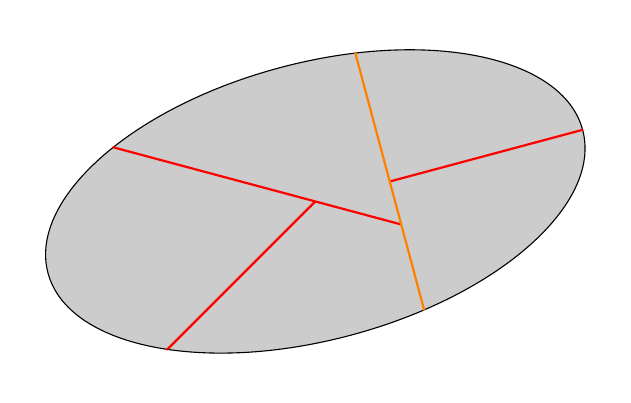
\begin{tikzpicture}[rotate=15,transform shape]
  \node[ellipse,draw=black,fill=gray,fill opacity=0.4,minimum height=100pt,minimum width=200pt] (e) at (0,0) {};
  \node[rotate=-15] (O) at ($(e.-60) + (0.3,-0.3)$){};
  \draw[thick,draw=red] (0,0) -- (e.-150) coordinate (e1);
  \draw[thick,draw=red] (0,0) -- ($(e.-30)!.29!(e.-210)$) coordinate (e2);
  \draw[thick,draw=red] (0,0) -- (e.-210) coordinate (e3);
  \draw[thick,draw=red] (e.0)-- ($(e.0)!0.36!(e.180)$) coordinate (e4);
  \draw[thick,draw=orange] (e.60) -- (e.-60) ;
  \end{tikzpicture}
  }
  \vspace{-3mm}
  \caption*{Two partitions of $\Omega$ into two yellow or five red sets}
 \end{center}
\end{figure}
	 Formulated in terms of $\sigma$-algebras the notion of more information for random variables is nothing else but saying $\sigma(X)\subseteq \sigma(Y)$. A good example to keep in mind is the random variable $Y$ that measures some temperature in tenth of a degree celsius and the random variable $X$ that measures the same temperature only in degrees.
	 \begin{luebung}
	 	Draw a picture of the partitions of $\Omega$ for the simple temperature example. What are $\sigma(X)$ and $\sigma(Y)$? Make sure you understand why $\sigma(X)\subseteq \sigma(Y)$ holds.
	 \end{luebung}	
	 
	 
%\vspace{-4mm}
%	\begin{figure}[h]
%	\begin{center}
%		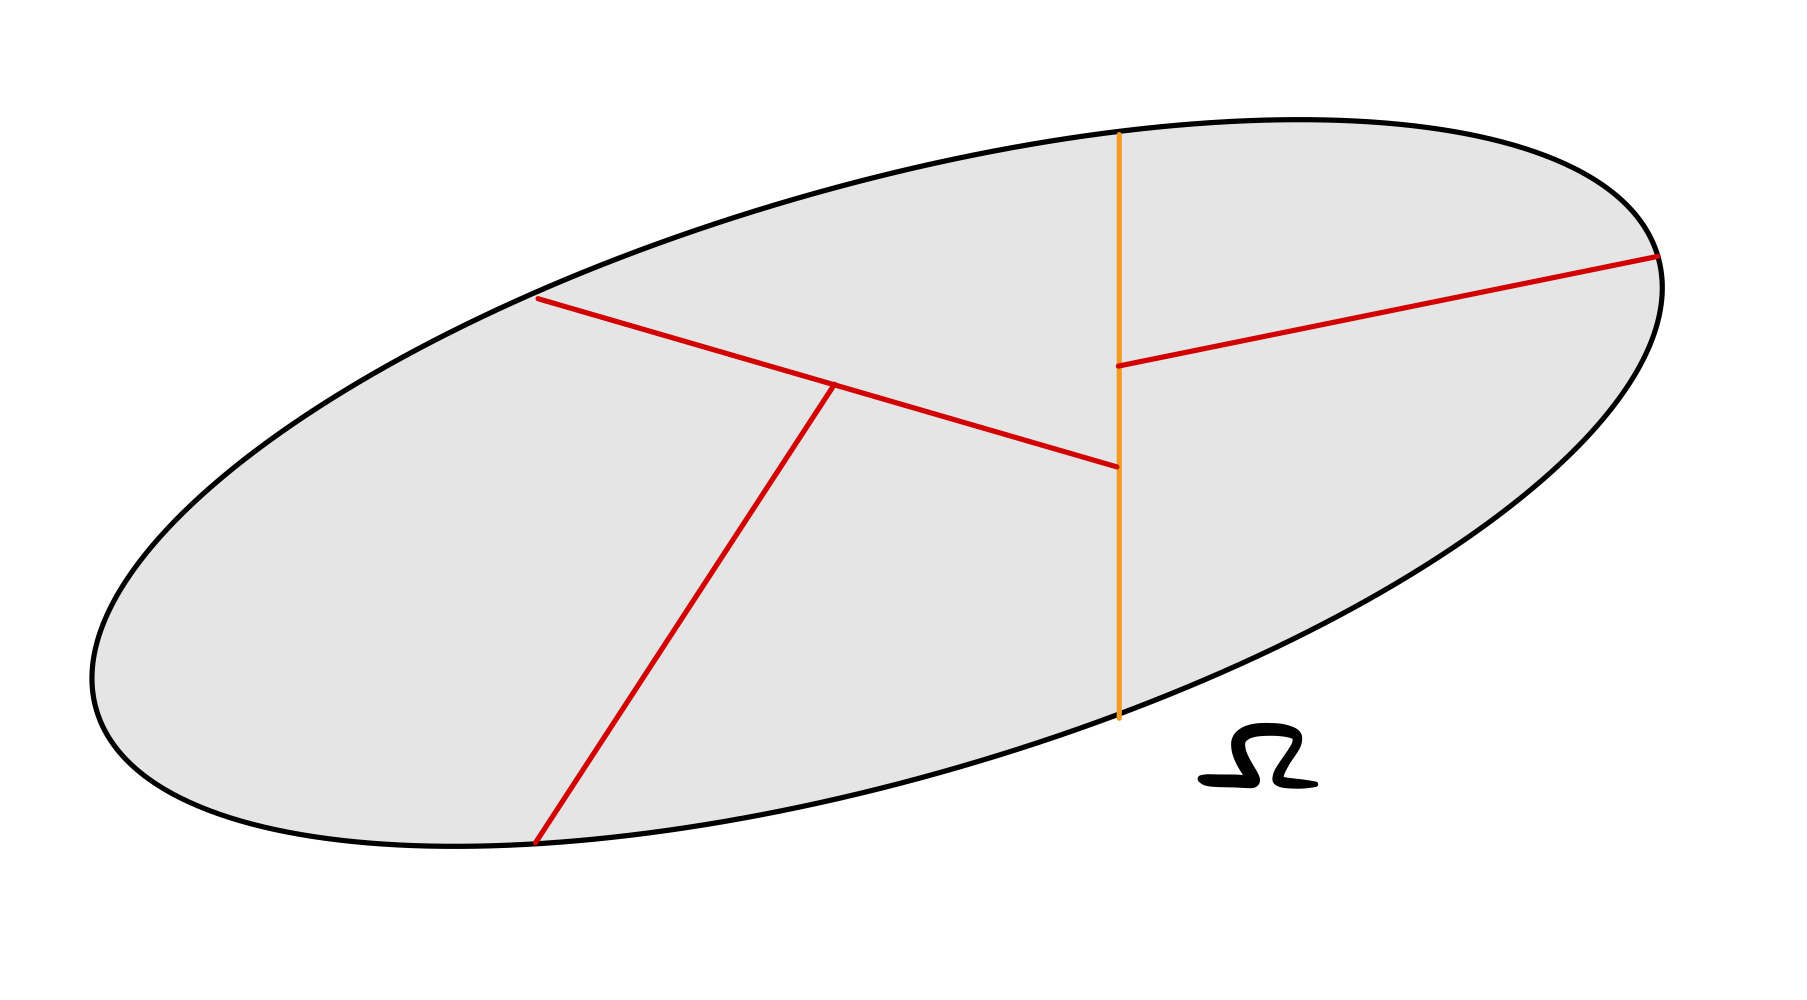
\includegraphics[scale=0.1]{CD0.jpeg}
%	\end{center}
%	\vspace{-1cm}
%	\caption*{Two partitions of $\Omega$, by two yellow or five red sets}
%	\end{figure}
	In mathematics it is important to chose examples which are not too simple and not too complicated in order to understand definitions. The best example to understand the concept of information of $\sigma$-algebras is probably the sequence of $\sigma$-algebras induced by a sequence of random variables. 
\begin{example}	
	Suppose $X_1,X_2,...$ is a sequence of random variables on $(\Omega, \mathcal A, \mathbb P)$, which we will later call a stochastic process. Then define
	\begin{align*}
		\mathcal F_n:=	\sigma(X_1,...,X_n):=\{ X_k^{-1}(B) : k\leq n,B\in \mathcal B(\R^n)\},\quad \text{ for }n\in\N.
	\end{align*}	
	It is clear from the definition that the sequence of $\sigma$-algebras $\mathcal F_n$ is increasing in the sense that $\mathcal F_n\subseteq \mathcal F_{n+1}$, thus, carries more and more "{}information"{}. Increasing sequences of $\sigma$-algebras will later-on be called filtrations. Let us assume, all $X_n$ are discrete random variables taking values in $\Z$ and check what "{}information"{} is carried by $\mathcal F_n$? Since everything is discrete we can write down all preimages to obtain simple generators of the $\sigma$-algebras:
		\begin{align*}
		\mathcal F_n
		&=\sigma(\{ \{X_1 \in A_1, ..., X_n \in A_n \} : A_i\subseteq \Z \})\\
		&=\sigma(\{\{X_1=i_1,..., X_n=i_n\}: i_k\in \Z \}).
	\end{align*}	
	Formulated in words, $\mathcal F_n$ is generated by events under which the process follows a given path, or, in other words, $\mathcal F_n$ contains all events which occurrence can be decided by looking at the first $n$ steps of the stochastic process. Increasing the time of the process thus leads to a larger set of observable events, thus, to more "{}information"{}. As an example let us check that the event "{}$0$ was hit before time $n$"{} belongs to $\mathcal F_n$ (but not to $\mathcal F_k$ for $k<n$):
	\begin{align*}
		&\quad \{0\text{ was hit before time }n\}\\
		&=\{0\text{ was hit at time }1\}\cup...\cup \{0\text{ was hit at time }n\}\\
		&= \bigcup_{i_2,i_3,...,i_n\in \Z} \{X_1= 0, X_2=i_2,..., X_n=i_n\}
		 \cup...\cup \bigcup_{i_1,...,i_{n-1} \in\Z} \{X_1= i_1, ..., X_{n-1}=i_{n-1},X_n=0 \}\\
		&\in \mathcal F_n.
	\end{align*}
	It is a good exercise to think of some other event and try to check that they belong (or do not belong) to the information of the first $n$ steps $\mathcal F_n$.
	
\end{example}
	These first thoughts comparing finitely many events break down immediately when the random variables fail to be discrete. To generalise we can only work with the generated $\sigma$-algebras
	\begin{align*}
		\sigma(X)=\{ X^{-1}(B): B\in \mathcal B(\R)\}.
	\end{align*}
	Recall that $\sigma(X)$ is the smallest $\sigma$-algebra on $\Omega$ so that $X$ is measurable. If $X$ is discrete $\sigma(X)$ only contains the events $\{X=a_k\}$ and their unions and complements. The discussion above suggests to say that $Y$ carries more "{}information"{} than $X$ if $\sigma(X)\subseteq \sigma (Y)$. To go even further, we can remove the concept of a random variable from the discussion. Similarly as above, we extend the idea of "{}information"{} to general $\sigma$-algebras by saying an $\sigma$-algebra $\mathcal F$ carries the "{}information"{} of its events. If $\mathcal B$ and $\mathcal F$ are $\sigma$-algebras on $\Omega$ we say that $\mathcal B$ carries more "{}information"{} than $\mathcal F$ if $\mathcal F\subseteq \mathcal B$. Recalling the motivation of $\sigma$-algebras comprising the observable events of the universe that makes perfect sense.\smallskip
	
The information that two $\sigma$-algebras are generated by random variables is extremely valuable. It allows to formalise the concept of more/less information in the following way:
\begin{lsatzwichtig}
\begin{lemma}[Doob's factorisation lemma]
		Let $X, Y$ two random variables on $(\Omega, \mathcal A, \mathbb P)$. If $X$ is measurable with respect to $\sigma(Y)$, i.e. $\sigma(X)\subseteq \sigma(Y)$, then there is a Borel-measurable mapping $h:\R\to\R$ such that $X=h(Y)$.
	\end{lemma}
\end{lsatzwichtig}
	\begin{proof}[Proof]
		Exercise. First understand the statement if $Y$ (and thus $X$) is discrete, $h$ can easily be written down. You can see that your $h$ can be defined arbitrarily for values that $Y$ does not take. Then approximate $Y$ using a sequence of step functions as in Theorem \ref{k} and use the appearing sequence of mappings $h_n$ to define $h$ as their pointwise limit.
	\end{proof}	
	\begin{lwarnhinweis}
		The function $h$ is not unique! Changing $h$ on values that $Y$ does not take will not change $h(Y)$.
	\end{lwarnhinweis}

	 A random variable $X$ carrying less "{}information"{} than another random variable $Y$ is thus only a transformation of $Y$ and as such, not more complicated than $Y$. In the example of measuring temperatures with different thermometers, depending on the thermometers, the mapping $h$ might just erase the decimals. The factorisation $h$ simplifies the more fine information $\{Y=5,0\}$, ..., $\{Y=5,9\}$ into one $\{X=5\}$.  The reverse statement does not hold. In the setting of the theorem there will usually not be a mapping $g$ such that $Y=g(X)$, the random variable $X$ cannot explain the random variable $Y$ without further information, think of measuring the temperature!\smallskip
	
	 Now suppose we are in a situation in which the factorisation does not apply but we would still like to express $Y$ as good as we can through $X$. Imagine $Y$ is a feature vector that we are interested in but we can only observe some simpler feature vector $X$ of which we believe $X$ should be able to explain $Y$ reasonably well. In statistics or machine learning you might have seen the idea of regressing $Y$ on $X$ in different contexts, such as finding a neural network functions such that $Y\approx f(X)$. In the following we discuss the measure theoretic version of this problem which is motivated from the factorisation lemma. If $Y$ cannot be written as $h(X)$ then at least we aim at finding a measurable function $h$ such that $Y\approx h(X)$ with a rigorously defined meaning of $\approx$. If we formalise $\approx$ through the $L^2$-distance of random variables, then - at least for square-integrable random variables - we can solve the minimisation problem using so-called conditional expectations. \smallskip
	 
	 
Before motivating conditional expectations through best approximation let us recall an elementary but important fact of expectations that should be familiar from Stochastik 2:
	
	
	
%	generated by a random vector $X=(X_1,...,X_n)$ or, equivalently, by random variables $X_1,...,X_n$. In probability we say that $\sigma(X)$ contains the "{}information"{} we get from $X$. But what does this mean? A real-valued random variable is a mapping that returns real values for each $\omega$ from the usually unknown source of all randomness $\Omega$. This is everything that potentially happens in the "{}universe"{}, but we are only able observe if the events $A\in \mathcal A$ happen or not. We can for instance not observe all collisions of atoms but we can observe certain more macroscopic events such as a tree falling or not. For the random variable $X$ the generated $\sigma$-algebra contains precisely those events that determine the outcome of $X$. For a better understanding let us consider the case of a discrete random variable taking values $a_1,...,a_N$ for which we have the simpler expression
%	\begin{align*}
%		\sigma(X)=\{ \cup_{i\in I} \{X= a_i\}: I\subseteq \{1,...,N\}\}=\sigma(\{\{X=a_i\}: i\in \{1,...,N\}\}).
%	\end{align*}
%	If $X$ only takes two values, the generated $\sigma$-algebra is $\{\Omega, \emptyset, \{X=a_1\}, \{X=a_2\}\}.$ The more complex (more possible outcomes) $X$ becomes, the larger the generated $\sigma$-algebra becomes. Similarly, if $X_1,...,X_n$ are all discrete random variables the generated $\sigma$-algebra 
	
%ANDERSRUM AUFSCHREIBEN. Erst erklaeren, was info sein sollte, dann beispiel, dann die erzeugte sigma-algebra erklaeren.	
\begin{lstep}
Given a random variable $X$, how would we best approximate $X$ by a constant value? As an instructive example, without any further thought, how would we approximate a $\mathcal N(\mu,\sigma^2)$-random variable best with a constant random variable? Of course using $Y\equiv \mu$, what else? To get the intuition straight let's check the $L^2$-approximation property of the expectation by solving
\begin{align*}
	\min_{\theta\in\R} \E[(X-\theta)^2].
\end{align*}
Expanding the square and minimising the quadratic function the solution to this simple approximation problem gives $\theta^*=\E[X]$. 
\end{lstep}
Here is a simple visualisation that will be useful for conditional expectations in a bit:
%	\begin{figure}[h]
%	\begin{center}
%		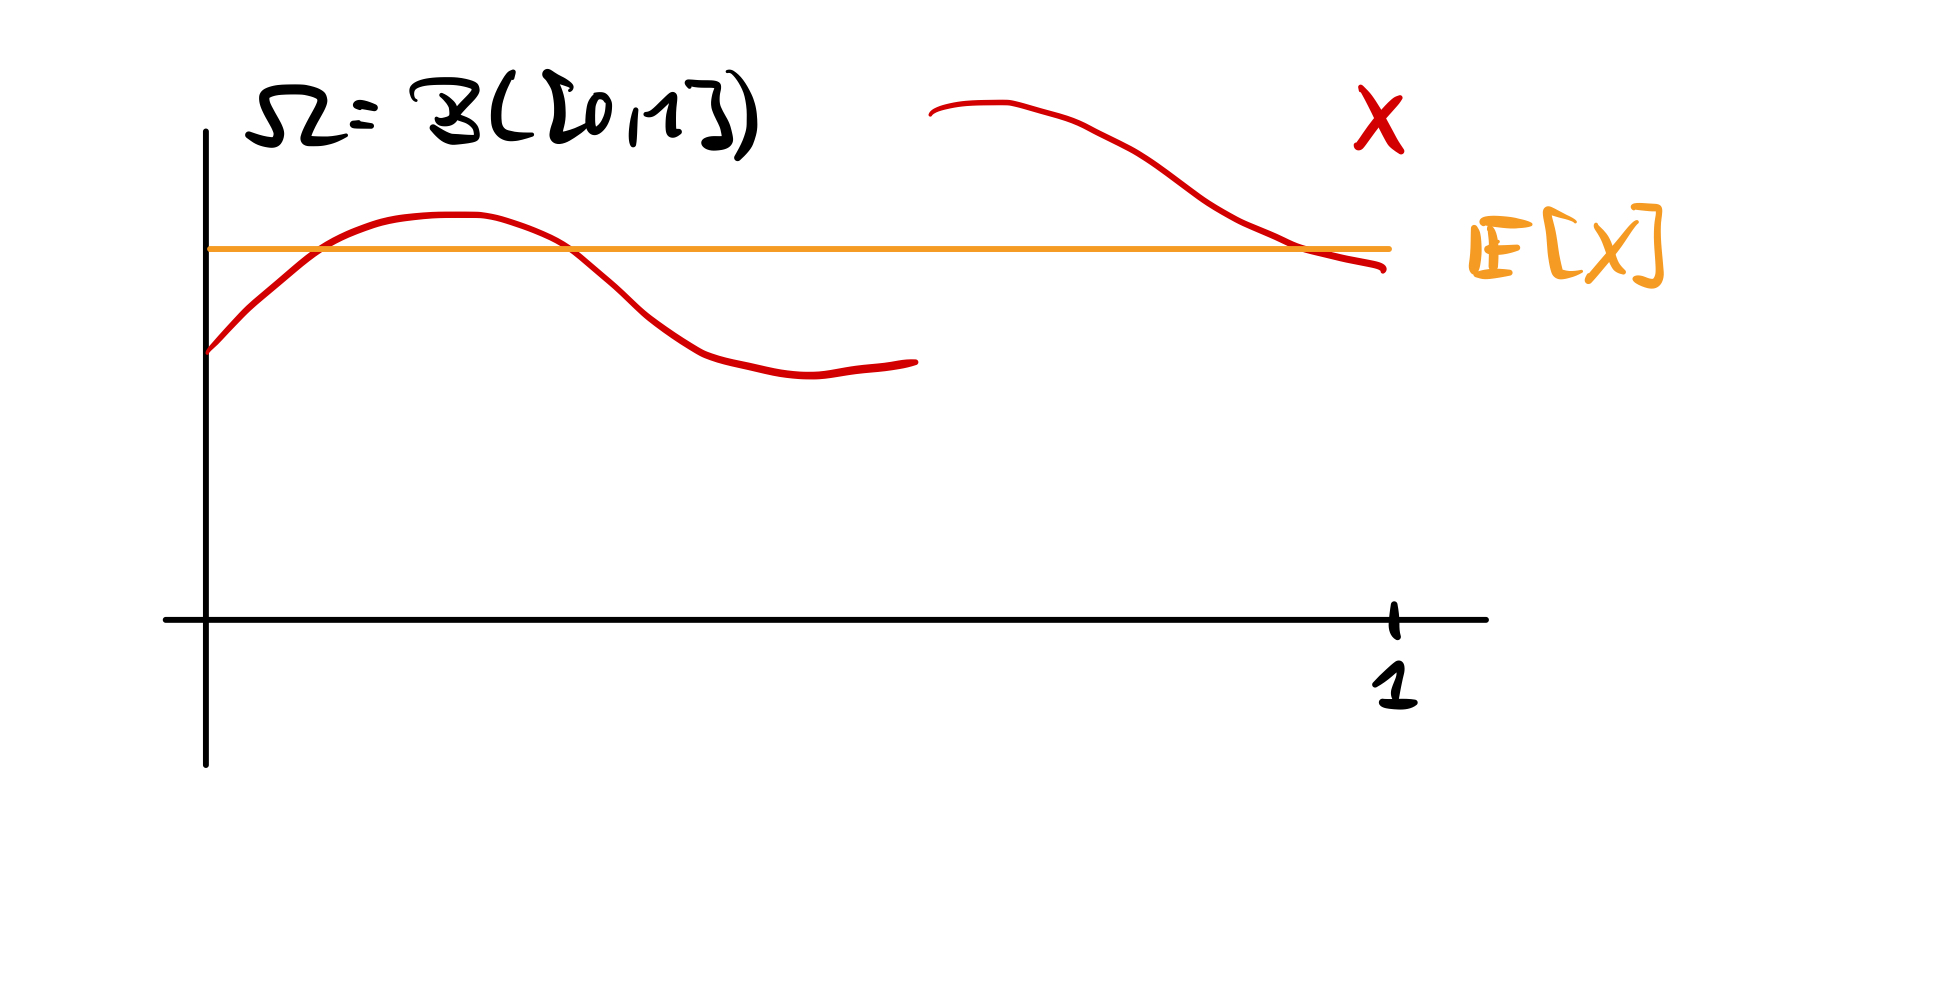
\includegraphics[scale=0.1]{CE4.jpeg}
%	\end{center}
%	\vspace{-1.3cm}
%	\caption*{Illustration of $L^2$-approximation of $X$ through the expectation}
%	\end{figure}

\begin{figure}[h]
\begin{center}
\scalebox{0.8}{
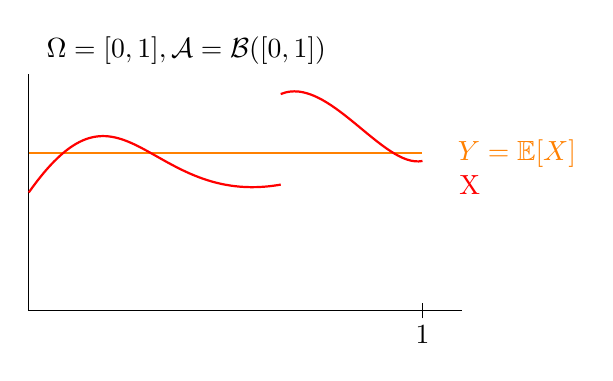
\begin{tikzpicture}
    \node at (2,3.3) (nodeO) {$\Omega=[0,1], \mathcal{A} = \mathcal{B}([0,1])$};
    \node[orange] at (6.2,2) (nodeA) {$Y=\mathbb{E}[X ]$};
    \node[red] (nodeX) at ($(nodeA.south)+(-0.6,-0.1)$) {X};
    \node (t1) at (5,-.3) {1};
    \draw (5,-.1) -- (5,.1);
    %AXIS Y
    \draw (0,0) -- ++(90:3cm);
    %AXIS X 
    \draw (0,0) --++(0:5.5cm);

    \draw[thick,orange](0,2) -- (5,2);
    \draw[thick,red]  (0,1.5) .. controls (1.2,3.2)  and (1.5,1.3) .. (3.2,1.6);
    \draw[thick,red]  (3.2,2.75) .. controls (3.8,3) and (4.5,1.8)  .. (5,1.9);
  \end{tikzpicture}
  }
  \vspace{-3mm}
  \caption*{Illustration of best $L^2$-approximation of $X$ through the expectation}
\end{center}
\end{figure}
\begin{lwarnhinweis}
Warning: People say "{}the best estimation of a random variable without further information is the expectation"{} but this is only correct if we talk about minimisation of the $L^2$-distance. Minimising $\E[|X-\theta|]$ leads to the median, not the expectation! \smallskip
\end{lwarnhinweis}

Let us now return to the approximation of random variables through random variables carrying less information, using the $L^2$-distance. Suppose we have a random variable $X$ on $(\Omega, \mathcal A, \mathbb P)$ and a discrete $\sigma$-algebra $\mathcal F\subsetneq \sigma(X)$, let's say $\mathcal F=\sigma(B_1,...,B_K)$ or, alternatively, $\mathcal F=\sigma(Y)$ for some random variable of the form $Y=\sum_{l=1}^K b_l \mathbf 1_{B_l}$. Now assume  we would like to explain $X$ as good as we can using only the "{}information"{} from $\mathcal F$ (or alternatively from $Y$). It is not possible to write $X=h(Y)$ as all $\mathcal F$-measurable functions take the form
\begin{align*}
	h(Y)= \sum_{l=1}^K h(b_l) \mathbf 1_{B_l}
\end{align*}
so that $X=h(Y)$ would contradict $\mathcal F\subsetneq \sigma(X)$. Instead, we try to best approximate $X$ by all $\mathcal F$-measurable random variables $\sum_{l=1}^K \beta_l \mathbf 1_{B_l}$, again in the $L^2$-sense as this is the easiest for computations.



\begin{figure}[h]
\begin{center}
  \hspace{10mm}
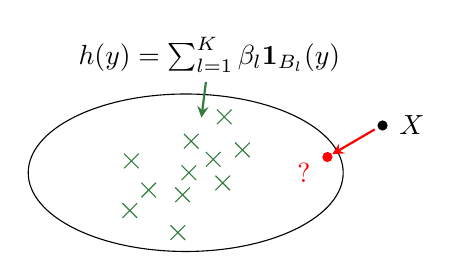
\begin{tikzpicture}
  \node at (0.3,0.5+1) (sum) {$h(y) = \sum_{l=1}^K \beta_l \mathbf{1}_{B_l}(y)$};
  \draw (0,0) ellipse (2 and 1);

\foreach \x/\n/\h in {0.07/a/0.40,0.35/b/0.17,-0.69/c/0.15,-0.04/d/-0.28,-0.47/h/-0.22,0.47/i/-0.13,0.72/j/0.29,-0.71/k/-0.48,0.49/l/0.71,-0.10/n/-0.76,0.04/o/0.00}{
    \node (\n)[circle,inner sep=2.5pt] at (\x,\h){};
    \draw[darkgreen] (\n.north west)--(\n.south east)(\n.south west)--(\n.north east);
}
  \draw[-stealth,darkgreen,thick] (sum) -- (0.2,0.7);
  \node[circle,inner sep=1.3pt,fill=black] (X) at (2.5,0.6) {} ;
  \node (x) at ($(X.east)+(0.3,-0)$) {$X$};
  \node (R) at (1.8,0.2) [circle,fill,inner sep=1.3pt,red]{};
  \node at (1.5,0) [red]{?};
  \draw[-stealth,red,thick] ($(X)+(-0.1,-0.05)$) -- (R);

  %%GUIDELINE
  %\draw[grey!50] (R) -- ++(0.7,0);
%  \draw[grey!50] (X) -- ++(0,-0.4);
  %%
  \end{tikzpicture}
  \vspace{-2mm}
 \caption*{Approximating X best from the set of all $\mathcal{F}$-measurable random variables}
\end{center}
\end{figure}
Let us solve the minimisation problem
\begin{align*}
	\min_{Z\, \mathcal F\text{-measurable}}\E[(X-Z)^2]
\end{align*}
without thinking much by just rewriting
\begin{align*}
	 \min_{Z\, \mathcal F\text{-measurable}}\E[(X-Z)^2]
	&=\min_{\beta_1,...,\beta_K} \E\Big[\Big(X-\sum_{l=1}^K \beta_l \mathbf 1_{B_l}\Big)^2\Big]\\
	&=\min_{\beta_1,...,\beta_K} \E\Big[\Big(\sum_{l=1}^K(X- \beta_l )\mathbf 1_{B_l}\Big)^2\Big]\\
	\overset{B_i\cap B_j=\emptyset}&{=}\min_{\beta_1,...,\beta_K} \sum_{l=1}^K\E\big[(X- \beta_l )^2 \mathbf 1_{B_l}\big]
\end{align*}
Minimising the right-hand side over the vector $\beta$ gives 
\begin{align*}
	\beta=\Big(\frac{\E[X \mathbf 1_{B_1}]}{\mathbb P(B_1)},...,\frac{\E[X \mathbf 1_{B_K}]}{\mathbb P(B_K)}\Big).
\end{align*} 
Introducing the notation $\E[X| A]:= \frac{\E[X \mathbf 1_{A}]}{\mathbb P(A)}$ we get the following solution of the $L^2$-approximation problem:
\begin{align}\label{cd1}
	Z^*=\sum_{l=1}^K \E[X| B_l] \mathbf 1_{B_l}.
\end{align} 
We will denote this random variable by $\E[X| \mathcal F]$ and call it the conditional expectation of $X$ given $\mathcal F$. $\E[X|\mathcal F]$ is the most we can say about $X$ (in the $L^2$-sense) with the information given by $\mathcal F$.
%	\begin{figure}[h]
%	\begin{center}
%		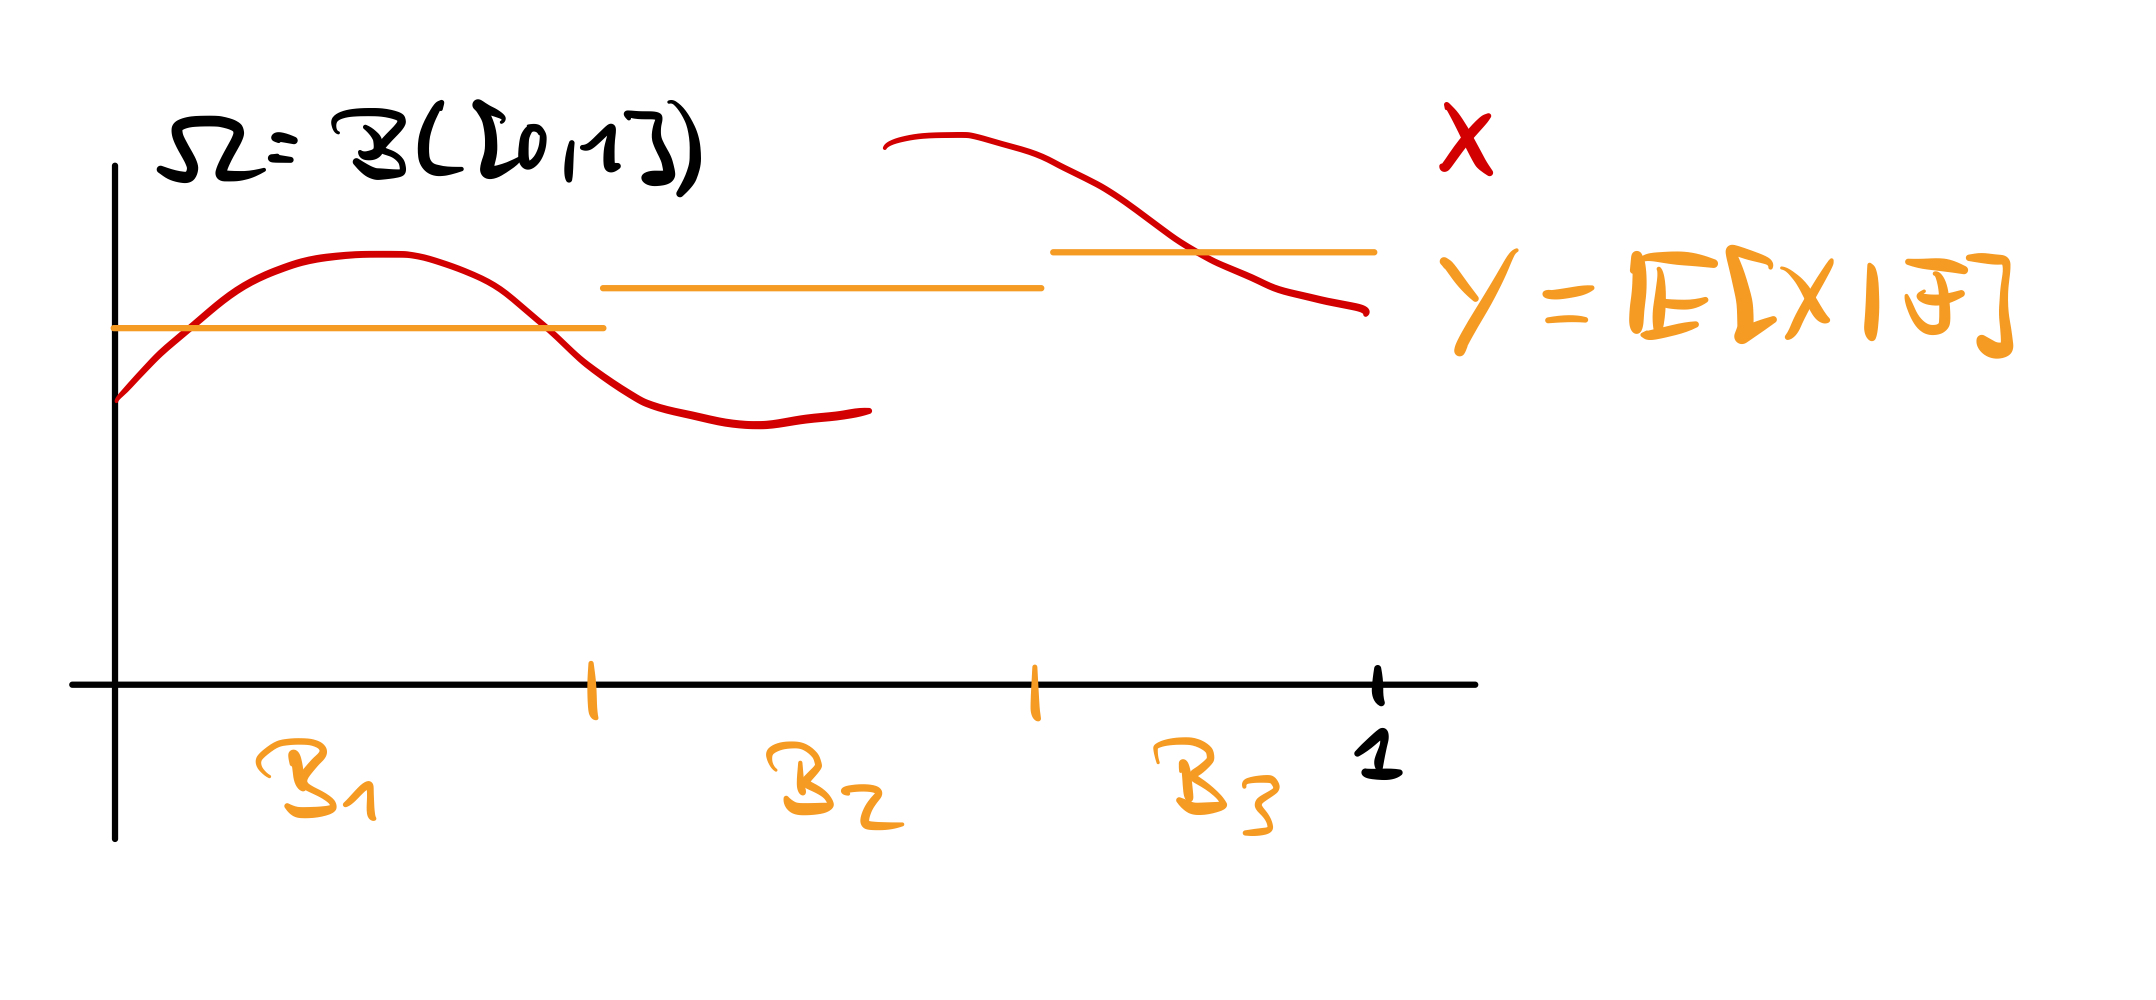
\includegraphics[scale=0.1]{CE2.jpeg}
%	\end{center}
%	\vspace{-1cm}
%	\caption*{Illustration of best $L^2$-approximation of $X$ through $\mathcal F$-measurable random variables}
%	\end{figure}

\begin{figure}[h]
\begin{center}
\scalebox{0.8}{
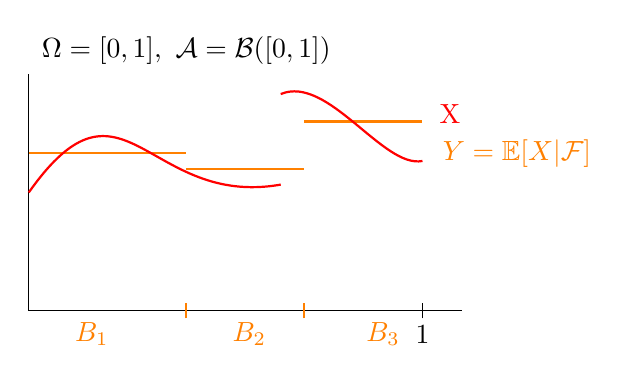
\begin{tikzpicture}
    \node (t1) at (5,-.3) {1};
    \draw (5,-.1) -- (5,.1);
    \draw ([yshift=-0.2]t1) -- ([yshift=0.2]t1) ;
    %AXIS Y
    \draw (0,0) -- ++(90:3cm);
    %AXIS X 
    \draw (0,0) --++(0:5.5cm);

    \node at (2,3.3) (nodeO) {$\Omega=[0,1], \ \mathcal{A} = \mathcal{B}([0,1])$};
    \node[orange] at (6.2,2) (nodeA) {$Y=\mathbb{E}[X| \mathcal{F}]$};
    \node[red] (nodeX) at (5.35,2.5) {X};
    \node[orange] at (0.8,-0.3) (B1) {$B_{1}$};
    \node[orange] at (2.8,-0.3) (B2) {$B_{2}$};
    \node[orange] at (4.5,-0.3) (B3) {$B_{3}$};
    
    %Y CURVE
    \draw[thick,orange](0,2) -- (2,2);
    \draw[thick,orange](2,1.8) -- (3.5,1.8);
    \draw[thick,orange](3.5,2.4) -- (5,2.4);

    \draw[thick, orange] (2,-0.1) -- (2,0.1);
    \draw[thick, orange] (3.5,-0.1) -- (3.5,0.1);
    %X CURVE
    \draw[thick,red] plot [smooth]  (0,1.5) .. controls (1.2,3.2)  and (1.5,1.3) .. (3.2,1.6);
    \draw[thick,red] plot [smooth]  (3.2,2.75) .. controls (3.8,3) and (4.5,1.8)  .. (5,1.9);
  \end{tikzpicture}
  }
  \vspace{-3mm}
    \caption*{Best $L^2$-approximation in the light of approximation through simple functions}
  \end{center}
\end{figure}
The computation above did not shed much light on what is going on. Could we have guessed the formula \eqref{cd1} without computations? For that sake let us recall the interpretation of elementary conditional probability measures $\mathbb P(\cdot \,|\, B):=\frac{\mathbb P(\cdot\, \cap B)}{\mathbb P(B)}$. The original random experiment is restricted to a subexperiment on $B$. All knowledge from $\Omega\backslash B$ is forgotten for the subexperiment, the relative probabilities of events $A\subseteq B$ remain unchanged by normalising all events with the same factor $\mathbb P(B)$. If $X$ was a random variable on $\Omega$ then the restriction to $ B$ is a random variable on the restriction $(B, \mathcal A_{|  B}, \mathbb P_{| B})$ with $\E_{| B}[X]=\E[X| B]$. We also call $\E_{|B}$ elementary conditional expectation. With this interpretation of elementary conditioning in mind formula \eqref{cd1} is nothing but $K$-times elementary $L^2$-approximation with constants for the $K$ restricted random variables $X_{|B}$. 
%	\begin{figure}[h]
%	\begin{center}
%		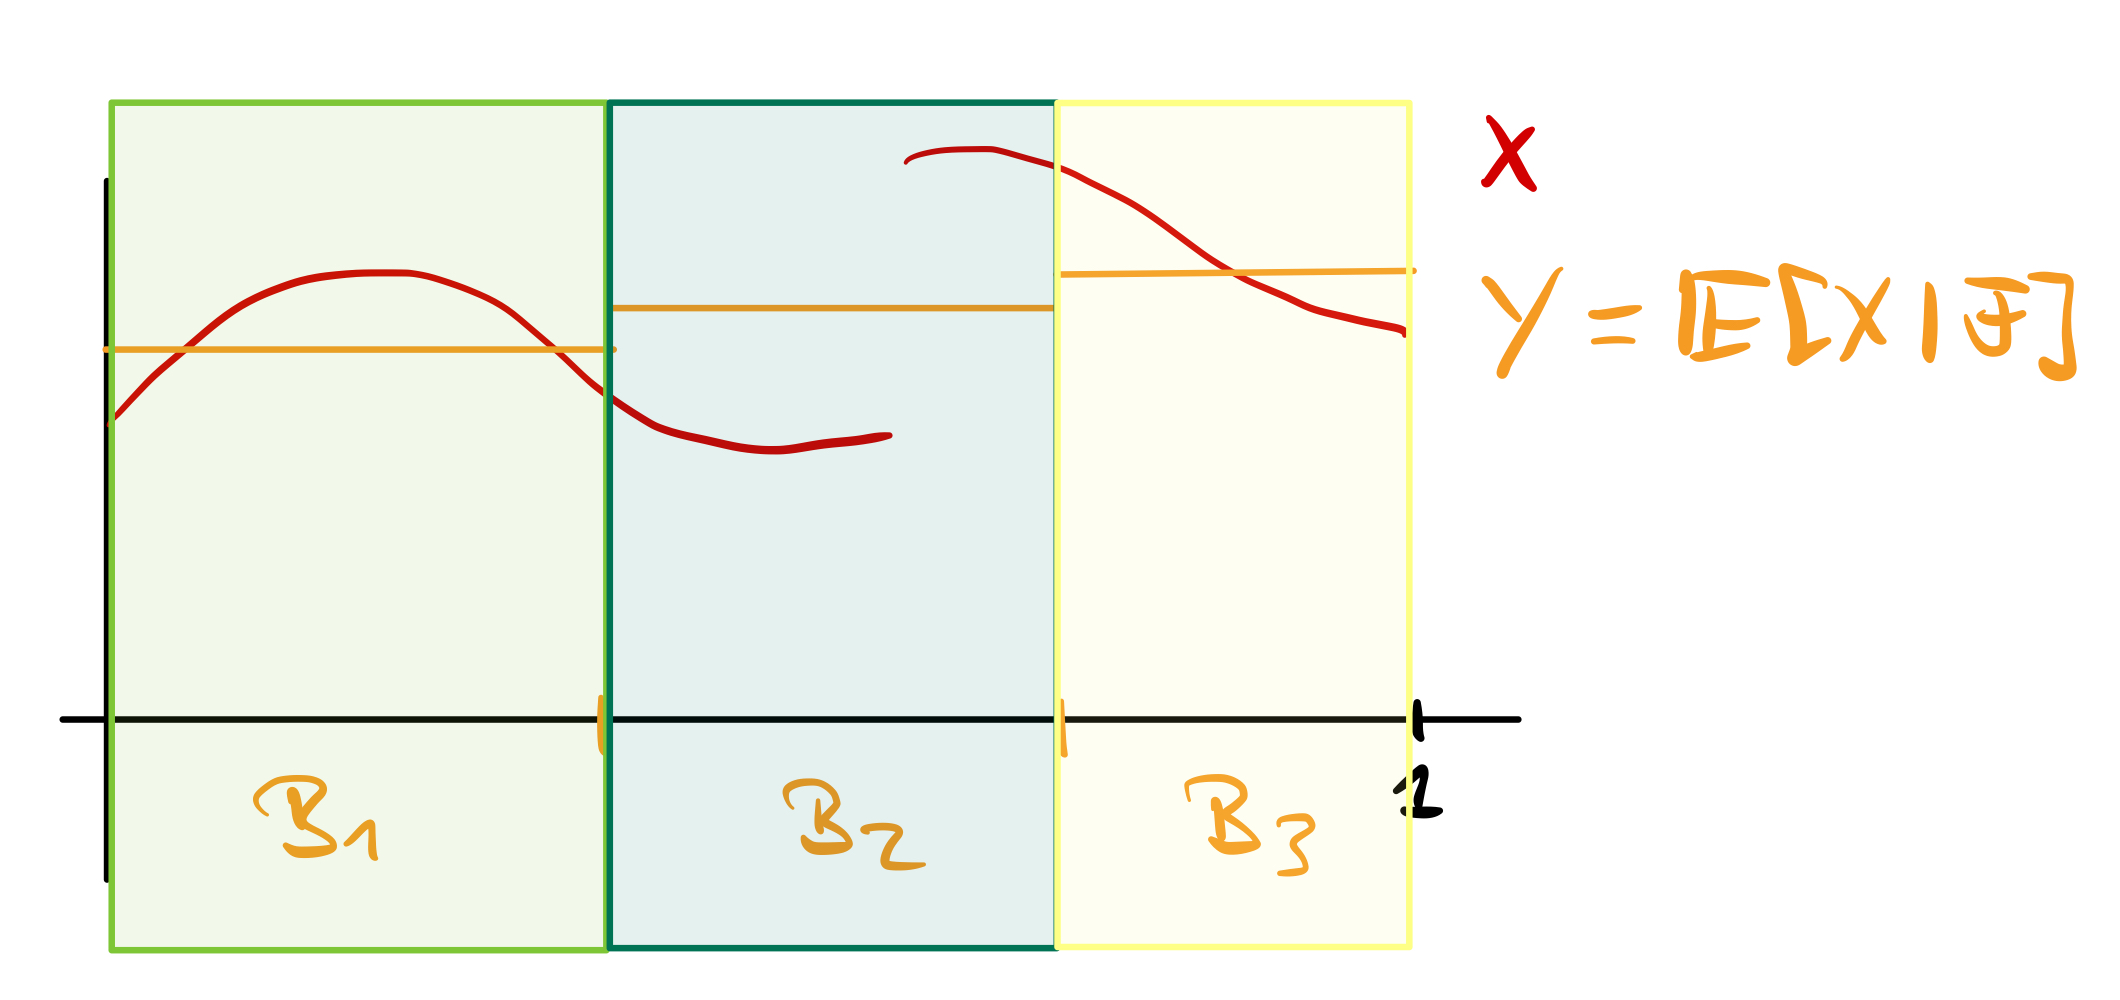
\includegraphics[scale=0.1]{CE5.jpeg}
%	\end{center}
%	\vspace{-0.7cm}
%	\caption*{Illustration of $L^2$-approximation through constant $L^2$-approximations of subexperiments}
%	\end{figure}

\begin{figure}[h]
\begin{center}
\scalebox{0.8}{
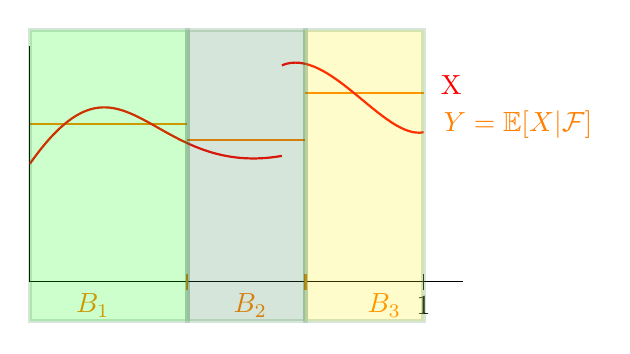
\begin{tikzpicture}
    \node (t1) at (5,-.3) {1};
    \draw (5,-.1) -- (5,.1);
    \draw ([yshift=-0.2]t1) -- ([yshift=0.2]t1) ;
    %AXIS Y
    \draw (0,0) -- ++(90:3cm);
    %AXIS X 
    \draw (0,0) --++(0:5.5cm);

    \node[orange] at (6.2,2) (nodeA) {$Y=\mathbb{E}[X| \mathcal{F}]$};
    \node[red] (nodeX) at (5.35,2.5) {X};

    \node[orange] at (0.8,-0.3) (B1) {$B_{1}$};
    \node[orange] at (2.8,-0.3) (B2) {$B_{2}$};
    \node[orange] at (4.5,-0.3) (B3) {$B_{3}$};

    \draw[thick, orange] (3.5,-0.1) -- (3.5,0.1);
    \draw[thick, orange] (2,-0.1) -- (2,0.1);

    \draw[thick,orange](0,2) -- (2,2);
    \draw[thick,orange](2,1.8) -- (3.5,1.8);
    \draw[thick,orange](3.5,2.4) -- (5,2.4);

    %X CURVE
    \draw[thick,red] plot [smooth]  (0,1.5) .. controls (1.2,3.2)  and (1.5,1.3) .. (3.2,1.6);
    \draw[thick,red] plot [smooth]  (3.2,2.75) .. controls (3.8,3) and (4.5,1.8)  .. (5,1.9);

    \draw[ultra thick,draw=darkgreen,fill=green,opacity=0.2]
      (0,-0.5) rectangle (2,3.2);

    \draw[ultra thick,draw=darkgreen,fill=darkgreen,opacity=0.2]
      (2,-0.5) rectangle (3.5,3.2);

    \draw[ultra thick,draw=darkgreen,fill=yellow,opacity=0.2]
      (3.5,-0.5) rectangle (5,3.2);
  \end{tikzpicture}
  }
 \caption*{Best $L^2$-approximation in the light of constant approximation on subexperiments}

  \end{center}
\end{figure}

Writing these thoughts formally by introducing $1=\sum_{l=1}^K \mathbf 1_{B_l}$ for the splitting the experiment into the $K$ subexperiments gives 
\begin{align*}
	\E[(X-Y)^2]&=\E\Big[\Big(\sum_{l=1}^K (X-\beta_l) \mathbf 1_{B_l} \Big)^2\Big]
	=\sum_{l=1}^K \E[(X-\beta)^2 \mathbf 1_{B_l}]=\sum_{l=1}^K \E_{|B_l}[(X-\beta_l)^2]\mathbb P(B_l).
\end{align*}
Best $L^2$-approximating all $K$ subexperiments by constants gives the same solution $\beta$ that we have found above by direct computation. The advantage is our better understanding of the appearing factors as elementary conditional expectations $\E_{|B_l}[X]$.\smallskip

In many textbooks on probability theory the motivation of conditional expectations is less formal, taking for granted that the best approximation of a random variable without extra information is the expectation. The intuitive reasoning is that the conditional expectation is the expectation given prior knowledge. Even though the statement "{}given"{} is very imprecise (the true formulation is $L^2$-minimisation as above) it works intuitively quite well. 
\begin{example}
	Suppose $X$ denotes a dice taking values $1,...,6$ with probabilities $\frac 1 6$. What is our best guess for $X$ if we know that the dice is even (or odd)? Keeping the $L^2$-minimisation property of expectations in mind we should  compute the expectations of the conditional experiments, the dice conditioned on being even (or odd). Intuitively, this is $4$ in the even and $3$ in the odd case. Denoting by $\mathcal F=\{\Omega, \emptyset, \{1,3,5\},\{2,4,6\}\}$ the additional information we have this is nothing but a sketch of the rigorous formula $$\E[X|\mathcal F]= \E[X|X \in \{1,3,5\} ] \mathbf 1_{X\in \{1,3,5\}}+\E[X|X\in \{2,4,6\}]\mathbf 1_{X\in \{2,4,5\}}$$ from above. Plug-in the definition of the elementary conditional expectations to check they give $3$ and $4$! 
\end{example}


There is a major challenge remaining. How do we generalise the above reasoning to general random variables and general $\sigma$-algebras if we cannot easily compute with finite sums of indicators? We follow the axiomatic approach of Kolmogorov in which the conditional expectations $\E[X|\mathcal F]$ and $\E[X|Y]$ are  defined through the two axiomatic properties
\begin{itemize}
	\item $\E[X|\mathcal F]$ is $\mathcal F$-measurable,
	\item $\E\big[\E[X|\mathcal F\big] \mathbf 1_A]=\E[X \mathbf 1_A]$ holds for all $A\in \mathcal F$.
\end{itemize}
Before discussing for general random variables how these properties define a reasonable object let us check that our discrete conditional expectation satisfies these properties. The measurability is a matter of our approach, we only minimised the distance over $\mathcal F$-measurable random variables. The more strange second property can be checked through the following quick computation. Let us first assume $A$ is equal to precisely one of the $B_l$, thus, disjoint from all the others:
\begin{align*}
	\E\big[ \E[X|\mathcal F] \mathbf 1_A\big]&=\E\Big[\sum_{l=1}^K \E[X|B_l]\mathbf 1_{B_l} \mathbf 1_A\Big]
	=\E\big[  \E[X|A] \mathbf 1_A\big]
	=\E[X|A] \E[\mathbf 1_A]
	\overset{\text{def}}{=} \E[X \mathbf 1_A].
%	&=\E\Big[  \E\Big[\sum_{n=1}^N \alpha_n \mathbf 1_{A_n}  \Big|A\Big] \mathbf 1_A\Big]\\
%	\overset{Lin., def.}&{=} \sum_{n=1}^N \E\Big[ \alpha_n \frac{\mathbb P(A_n\cap A)}{\mathbb P(A)}\mathbf 1_A\Big]\\
%	\overset{Lin.}&{=}\sum_{n=1}^N \alpha_n \mathbb P(A_n\cap A)\\
%	&=\E\Big[\sum_{n=1}^N \alpha_n \mathbf 1_{A_n }\mathbf 1_A\Big]
\end{align*}
Since all $A\in \mathcal F$ can be written as finite union of the $B_k$ the general claim follows from linearity.\smallskip

The magic of conditional expectation is that the preceding two properties are all we need for a powerful definition of general conditional expectation with amazing consequences!


\section{The axiomatic approach of Kolmogorov}


We shall now turn to a general setup, dropping the assumption of discrete random variables and finite $\sigma$-algebras. We will reverse the story and start with an axiomatic definition of conditional expectation from which we then derive abstract existence and identify key properties (such as $L^2$-error minimization) that reflect the motivation given before. 

\begin{ldefwichtig}
\begin{deff}\label{deff_condexp}
	Let $(\Omega, \mathcal A, \mathbb P)$ a probability space, $X\in \mathcal L^1(\Omega, \mathcal A, \mathbb P)$, and $\mathcal F$ a sub-$\sigma$-Algebra of $\mathcal A$. Then a random variable $Z$  on $(\Omega, \mathcal A, \mathbb P)$ is called the \textbf{conditional expectation of $X$ given $\mathcal F$} if
	\begin{itemize}
		\item $Z$ is $\mathcal F$-measurable,
		\item $\mathbb E[Z \mathbf 1_A]=\mathbb E[X \mathbf 1_A]$ for all $A\in \mathcal F$.
	\end{itemize}
	If such a random variable $Z$ exists, then we write $Z=E[X|\mathcal F]$. If $\mathcal F=\sigma(Y)$ for a  random variable $Y$ then we write $Z=\E[X|Y]$ and call $Z$ the \textbf{conditional expectation of $X$ give $Y$}.
\end{deff}
\end{ldefwichtig}
Choosing $A=\Omega$ in the second condition it is clear that the integrability assumption on $X$ cannot be avoided. In contrast to the section before we cannot use $L^2$-distances, second moments are not assumed to be finite. It is important to note that the very definition of $\E[X|\mathcal F]$ shows that conditional expectation is not defined uniquely. This is caused by the second property as expectations do not change if random variables are changed on zero sets. Any other $\mathcal F$-measurable random variable $\bar Z$ that equals $Z$ almost surely will automatically satisfy the second condition.
\begin{ldef}
\begin{deff}
	Suppose $Z$ and $\bar Z$ are random variables on a probability space $(\Omega, \mathcal A, \mathbb P)$. We call $\bar Z$ a \textbf{version} of $Z$ if $\mathbb P(Z=\bar Z)=1$.
\end{deff}
\end{ldef}
We will see later that it can be useful to choose particularly versions of the conditional expectation that satisfies additional measurability properties.

\begin{lsatzwichtig}
\begin{theorem}\label{existenceCE}
	Let $X$ an integrable random variable on $(\Omega, \mathcal A, \mathbb P)$ and $\mathcal F$ a sub-$\sigma$-algebra of $\mathcal A$. Then the conditional expectation $\E[X|\mathcal F]$ exists and is almost surely unique, i.e. two random variables satisfying the two defining properties are versions of each other.
\end{theorem}
\end{lsatzwichtig}
\begin{proof}[Proof]
	\textbf{Uniqueness:} Suppose $Z$ and $\bar Z$ are random variables fulfilling the two defining properties of Definition \ref{deff_condexp} and let $A=\{\bar Z<Z\}\in\mathcal{F}.$ Using the second property of conditional expectation, it holds that 
	$$0=\E[\mathbf{1}_AZ]-\E[\mathbf{1}_A\bar{Z}]=\E[(Z-\bar{Z})\mathbf{1}_A]\ge0.$$ It follows that $\mathbf{1}_A(Z-\bar{Z})=0$ almost surely. Similarly, it holds that $\mathds{1}_{A^c}(Z-\bar{Z})=0$ almost surely. Taking the unions of the nullsets gives $Z=\bar Z$ almost surely.\smallskip
	
	\textbf{Existence:} To prove the existence we use the Radon-Nykodyn from functional analysis. The theorem states that a $\sigma$-finite measure $\nu$ has a density with respect to another $\sigma$-finite measure $\mu$ if and only if $\nu\ll \mu$. Here we use the absolutely continuity notion $\mu\ll \mu$ if every zero set for $\mu$ is also a zero set for $\nu$. The interested reader is referred any book containing enough Functional Analysis \footnote{For instance P. Billingsley, 1995, "{}Probability and Measure"{} (3rd edition), Wiley, pp. 419–427}. Now let 
	\begin{align}\label{eq_05}
		Q^+:\cF\to[0,1],A\mapsto\E[X^+\mathbf{1}_A]\quad\text{ and }\quad Q^-:\cF\to[0,1],A\mapsto\E[X^-\mathbf{1}_A],
	\end{align}
	which are both $\sigma$-finite measures on $\mathcal F$ with $Q^+\ll \mathbb P$ and $Q^-\ll \mathbb P$. Hence, there are $\mathcal{F}$-measurable densities $Z^+,Z^-$ with $$Q^+(A)=\int_A Z^+\dint\mathds{P}\quad \text{ and }\quad Q^-(A)=\int_A Z^-\dint\mathds{P}$$ for all $A\in\cA$. Let $Z:=Z^+-Z^-$, then $Y$ is $\cF$ measurable and 
	\begin{align*}
		\E[\mathbf{1}_AZ]&=\E[\mathbf{1}_AZ^+]-\E[\mathbf{1}_AZ^-]\\
		&=\int_AZ^+\dint\mathds{P}-\int_AZ^+\dint\mathds{P}\\
		&\overset{\eqref{eq_05}}=Q^+(A)-Q^-(A)\\
		&=\E[\mathbf{1}_AX^+]-\E[\mathbf{1}_AX^-]\\
		&=E[\mathbf{1}_AX].
	\end{align*}
	Therefore, the random variable $Z$ fullfills the properties of the conditional expectation of $X$ given $\cF$.
\end{proof}
	\marginpar{\textcolor{red}{Lecture 2}}


Just as for typical expectations we continue with a set of properties fulfilled by the conditional expectation. Some properties look familiar to old properties of expectations, but always keep in mind: conditional expectations are random variables! 

\begin{lsatzwichtig}
\begin{theorem}[Standard properties of conditional expectation]\label{cond_properties}
	Let $X,Y\in\cL^1(\Omega,\cA,\mathbb{P})$, $\lambda\in \R$, and $\cG\subseteq\cF\subseteq\cA$ sub-$\sigma$-Algebras. Then the following properties hold:
		\begin{enumerate}[label=(\roman*)]
			\item $\E\big[\E[X\,|\,\mathcal F]\big]=\E[X]$ and  $\E[1\,|\, \mathcal F]=1$ a.s.
			\item $\mathds{E}[\,\lambda X+Y \,|\, \mathcal{F}\,]=\lambda\mathds{E}[\, X \, | \, \mathcal{F}\, ]+\mathds{E}[Y \, | \, \mathcal{F}]$ a.s.
			\item $X \geq Y$ a.s. $\Rightarrow \mathds{E}[X\, |\, \mathcal{F}] \geq \mathds{E}[Y \,|\, \mathcal{F}]$ a.s.
			\item If $\mathds{E}[\lvert XY \rvert] < \infty$ and $Y$ is $\mathcal{F}$-measurable, then
				$$\mathds{E}[XY\,|\,\cF] = Y\mathds{E}[X\,|\,\cF]\:\:\text{a.s.}\quad \text{ and }\quad \mathds{E}[Y\,|\,\cF]=Y\:\:\text{a.s.}$$
			\item $\mathds{E}\big[\mathds{E}[X\,|\,\cF]\,\big|\,\cG\big] = \mathds{E}\big[\mathds{E}[X\,|\,\cG]\,\big|\,\cF\big]=\mathds{E}[X\,|\,\cG]$ a.s.
			\item $\big\lvert\mathds{E}[X\,|\,\cF]\big\rvert \leq \mathds{E}\big[\lvert X \rvert\,\big|\,\cF\big]$ a.s.
			\item If $\sigma(X)$ and $\cF$ are independent, then $\mathbb E[X\,|\,\cF] = \mathbb E[X]$ a.s.
			\item If $\mathbb{P}(A)\in \{0,1\}$ for all $A \in \cF$, then $\mathbb E[X\,|\,\cF] = \mathbb E[X]$ a.s.
			\item If $\E[X|\mathcal F]$ is a.s. constant, then $\E[X|\mathcal F]=\E[X]$ a.s.
			\item If $\E[X\mathbf 1_A]=\E[Y\mathbf 1_A]$ for all $A\in \mathcal F$, then $\E[X|\mathcal F]=\E[Y|\mathcal F]$ a.s.
			\item Suppose $\lvert X_n \rvert \leq Y$ a.s. for $Y \in \cL^1(\Omega, \mathcal A, \mathbb P)$ and $\lim\limits_{n \to \infty}X_n = X$ a.s., then
				$$\lim\limits_{n \to \infty}{ \mathbb E[X_n\,|\,\cF]}=\mathbb E[X\,|\,\cF] \,\,\text{ a.s and in }L^1.$$ 
			\item Suppose $X_n\geq 0$ is an increasing sequence of random variables with $\lim_{n\to\infty} X_n=X$ a.s., then 
				$$\lim\limits_{n \to \infty}{ \mathbb E[X_n\,|\,\cF]}=\mathbb E[X\,|\,\cF] \,\,\text{ a.s}.$$ 			
				
	\end{enumerate}
\end{theorem}
\end{lsatzwichtig}
\begin{proof}[Proof]
	\begin{enumerate}[label=(\roman*)]
		\item Exercise
		\item The trick is always the same: If we intend to prove $\E[...|...]=Z$ a.s., we need to check for $Z$ the two defining properties of the claimed conditional expectation. Uniqueness of conditional expectations then implies that $Z$ is a version of the conditional expectation. Following once in detail this routine let us denote the righthand side by $Z$. Since $Z$ is a linear combination of two $\mathcal F$-measurable random variables, $Z$ is $\mathcal F$-measurable, which is the first condition of conditional expectation. For the expectation condition, with $A\in\mathcal F$, we obtain, using properties of the usual expectation (linearity and (ii) of Theorem \ref{S7}) and the second property of the conditional expectations $\E[X\,|\,\mathcal F]$, $\E[Y\,|\, \mathcal F]$,
			\begin{align*}
				\E[\mathbf 1_A Z F]&=\mathbb E[\mathbf{1}_A(\lambda\mathds{E}[\, X \, | \, \mathcal{F}\, ]+\mathds{E}[Y \, | \, \mathcal{F}])]\\
				&=\lambda\mathbb E[\mathbf{1}_A\mathbb E[X\,|\,\cF]]+\mathbb E[\mathbf{1}_A\mathbb E[Y\,|\,\cF]]\\
					&=\lambda\mathbb E[\mathbf{1}_A X]+\mathbb E[\mathbf{1}_A Y]\\
					&=\mathbb E[\mathbf 1_A (\lambda X+Y)].
			\end{align*}
			Hence, $Z$ satisfies the defining conditions of $\E[\lambda X+Y\, |\, \mathcal F]$.
		\item \label{ii} Lemma \ref{me} tells us that $A:=\lbrace\mathbb E[X|\cF]<\mathbb E[Y|\cF]\rbrace\in \cF$. Using monotonicity of expectations and linearity of conditional expectations from (ii) gives
			$$0 \geq \mathbb E[\mathbf 1_A (\mathbb E[X\,|\,\cF]-\mathbb E[X\,|\,\cF])] =\mathbb E[\mathbf 1_A \mathbb E[X-Y\,|\,\cF]] = \mathbb E[\mathbf 1_A (X-Y)]\overset{\text{ass.}}{\geq} 0.$$ Since $\mathbf 1_A (\mathbb E[X\,|\,\cF]-\mathbb E[Y\,|\,\cF]) \leq 0$ by definition of $A$ we find $\mathbf 1_A (\mathbb E[X\,|\,\cF]-\mathbb E[Y\,|\,\cF]) = 0$ a.s. (Theorem \ref{S7}, (iii)) which gives $\mathbf 1_A = 0$ a.s. or, equivalently, $\mathbb E[X\,|\,\cF]\geq\mathbb E[Y\,|\,\cF]$ a.s.
		\item The proof works through discretisation and linearity. First assume $X,Y\geq 0$. Define $Y_n = \frac{1}{2^n} \cdot \lfloor 2^n \cdot Y \rfloor$ (draw a picture to undestand it!) so that almost surely $Y_n \nearrow Y$ and $$Y_n \mathbb E[X\,|\,\cF] \nearrow Y \mathbb E[X\,|\,\cF].$$ MCT for usual expectations implies $\lim \limits_{n \to \infty}\mathbb E[\mathbf 1_A Y_n \mathbb E[X\,|\,\cF]]=\mathbb E[\mathbf 1_A Y \mathbb E[X\,|\,\cF]]$ for $A\in\cF$. Now we compute the left-hand side:
			\begin{align*}
				\mathbb E\left[\mathbf 1_A Y_n \mathbb E[X\,|\,\cF]\right]&=\mathbb E\bigg[\mathbf 1_A \sum_{k=0}^\infty \frac{k}{2^n}\mathbf 1_{Y_n=\frac{k}{2^n}}\mathbb E[X\,|\,\cF]\bigg] \\
				\overset{\text{MCT}}&{=} \sum_{k=0}^\infty\mathbb E\bigg[\mathbf 1_A \frac{k}{2^n}\mathbf 1_{Y_n=\frac{k}{2^n}}\mathbb E[X\,|\,\cF]\bigg]\\
				&= \sum_{k=0}^\infty\mathbb E\bigg[\mathbf 1_A \frac{k}{2^n}\mathbf 1_{Y_n=\frac{k}{2^n}} X\bigg]\overset{\text{MCT}}{=}\mathbb E[\mathbf 1_A Y_n X]
			\end{align*}
			Again MCT yields $\mathbb E[\mathbf 1_A Y X]=\mathbb E[\mathbf 1_A Y \mathbb E[X\,|\,\cF]]$ which shows the expectation condition $$\mathbb E[Y X\,|\,\cF]=Y \mathbb E[X\,|\,\cF].$$ The $\mathcal F$-measurability of $Y\E[X|\mathcal F]$ follows from measurability of products.
			For the general case we proceed as usually, writing $X=X^+ - X^-$,$Y=Y^+ - Y^-$ and then using linearity from (ii). The second claim follows from (i) using $X=1$.
		\item Exercise
		\item The proof is exactly the same that we have already encountered for the classical expectation in Lemma \ref{properties}:
			\begin{align*}
				\big\lvert \mathbb E[X\,|\,\cF] \big\rvert &= \big\lvert \mathbb E[X^+\,|\,\cF]-\mathbb E[X^-\,|\,\cF]\big\rvert \\ 
				\overset{\Delta}&{\leq} \big \lvert \mathbb E[X^+\,|\,\cF] \big\rvert + \big\lvert \mathbb E[X^-\,|\,\cF] \big\rvert \\
				&= \mathbb E[X^+\,|\,\cF] + \mathbb E[X^-\,|\,\cF] \\
				&= \mathbb E[X^+ + X^-\,|\,\cF] \\
				&= \mathbb E\big[\lvert X \rvert \,\big|\,\cF\big]
			\end{align*}
		\item First recall that one (of several equivalent) ways to state the independence is to say that $X$ is independent of $\mathbf 1_A$ for all $A\in \mathcal F$. Using the factorisation of expectations of independent random variables gives
						\[	\mathbb E[\mathbf 1_A X] \overset{\text{ind.}}{=} \mathbb E[X]\mathbb E[\mathbf 1_A] \overset{\text{lin.}}{=} \mathbb E[\mathbb E[X]\mathbf 1_A] \]		
		for all $A\in \mathcal F$. Since additionally all constant random variables are $\mathcal F$-measurable, $\E[X]$ is a version of $\E[X\,|\, \mathcal F]$.

		\item The "trivial"{} $\sigma$-algebra $\cF$ is independent of all sub-$\sigma$-algebras $\cA$, in particular of $\sigma(X)$. Now use (vii).
		\item Suppose $\E[X|\mathcal F]=c$ almost surely. The defining property yields $\E[X\mathbf 1_A]=\E[ c\, \mathbf 1_A]=c\, \P(A)$ for all $A\in \mathcal F$. Now choose $A=\Omega$ and the claim follows.
		\item We show that $\E[Y|\mathcal F]$ satisfies the defining properties of $\E[X|\mathcal F]$ and then apply the uniqueness. Measurability follows from the measurability of conditional expectations, the expectation property as follows:
		\begin{align*}
			\E[X\mathbf 1_A]=\E[Y\mathbf 1_A]\overset{(i)}{=}\E\big[\E[Y\mathbf 1_A|\mathcal F]\big]\overset{(iv)}{=}\E\big[\E[Y|\mathcal F]\mathbf 1_A\big],\quad \forall A\in \cF.
		\end{align*}
		\item Define $Z_n = \sup\limits_{k\geq n}\lvert X_k - X \rvert$ so that $0\leq Z_n \leq 2Y$ and $Z_n \rightarrow 0,n \rightarrow \infty$. By usual DCT we find $\mathbb E[Z_n]\rightarrow 0$ for $n \rightarrow \infty$. The $L^1$-convergence can now be deduced as
				\begin{align*}
					\mathbb E\big[\lvert \mathbb E[X_n\,|\,\cF]-\mathbb E[X\,|\,\cF]\rvert\big]
					\overset{\Delta}{\leq} \mathbb E\big[\mathbb E[\lvert X_n - X \rvert \,|\,\cF]\big] = \mathbb E[\lvert X_n - X \rvert] \rightarrow 0,\quad n \rightarrow \infty
				\end{align*}
Next, towards the almost sure convergence. Since $Z_n$ is decreasing in $n$ the monotonicity implies that $\mathbb E[Z_n\,|\,\cF]$ is decreasing. Denote the limit by $M$. With Fatou we get $$0 \leq \mathbb E[M] \leq \liminf\limits_{n \rightarrow \infty}\mathbb E[\mathbb E[Z_n\,|\,\cF]]= \liminf\limits_{n \rightarrow \infty}\mathbb E[Z_n] = 0.$$ Hence, $M = 0$ a.s. Finally, we can conclude $$0\leq \lim_{n\to\infty} \lvert \mathbb E[X_n\,|\,\cF]-\mathbb E[X\,|\,\cF]\rvert \leq \lim_{n\to\infty} \mathbb E[Z_n\,|\,\cF] = M = 0.$$
	\item Using the monotonicity yields that $0\leq \E[X_n|\mathcal F]\leq \E[X_{n+1}|\mathcal F]\leq ...\leq \E[X|\mathcal F]$ so there is an almost sure limit $V:=\lim_{n\to\infty} \E[X_n|\mathcal F]$ and $V\leq \E[X|\mathcal F]$. Define $B=\{V<\E[X|\mathcal F]\}$, then
	\begin{align*}
		\E\big[ \E[X|\mathcal F] \mathbf 1_B\big]
		\overset{B\in \mathcal F}&=	\E[X \mathbf 1_B]\\
		\overset{\text{MCT}}&{=} \lim_{n\to\infty} \E[X_n \mathbf 1_B]\\
				\overset{(i)}&{=} \lim_{n\to\infty} \E\big[\E[X_n \mathbf 1_B|\mathcal F]\big]\\
		\overset{B\in \mathcal F}&=\lim_{n\to\infty} \E\big[\E[X_n |\mathcal F]\mathbf 1_B\big]\\
		\overset{\text{MCT}}&{=} \E[V\mathbf 1_B]\\
	\end{align*}
	But then $\P(B)$ must be $0$ as otherwise the equalities could not hold.	
	\end{enumerate}
\end{proof}
\begin{lsatz}
\begin{theorem}[Jensen's inequality for conditional expectation]
	Suppose $\varphi$ is convex with $X,\varphi (X) \in \mathcal L^1(\Omega,\cA,\mathds P)$, then
		\begin{align*}
			\varphi\big(\mathbb E[X\,|\,\cF]\big) \leq \mathbb E[\varphi(X)\,|\,\cF] \:\: \text{ a.s}.
		\end{align*}
\end{theorem}
\end{lsatz}
\begin{proof}[Proof]
			
	Let $E_\varphi=\lbrace (a,b)\in \mathbb{R}^2:\varphi(x)\geq ax+b,\forall x\rbrace$ the set of all subtangents. Then one (of many) ways to express the convexity is the expression
		\begin{align*}
			\varphi(x) = \sup\limits_{(a,b)\in E_\varphi}(ax+b) = \sup\limits_{(a,b)\in E_\varphi \cap \mathbb{Q}^2}(ax+b)
		\end{align*}



\begin{figure}[h]
\begin{center}

\scalebox{0.8} {
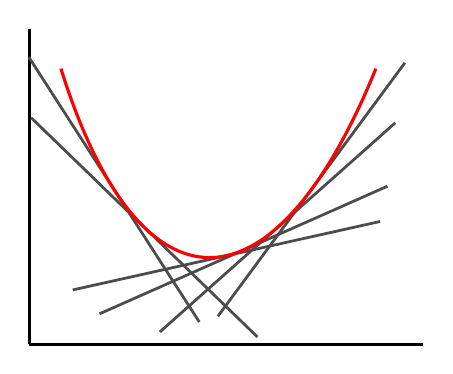
\begin{tikzpicture}
    %AXIS Y
    \draw[black,line width=0.4mm] (0.5,0) -- ++(90:4cm);
    %AXIS X 
    \draw[black,line width=0.4mm] (0.5,0) --++(0:5cm);
    % CURVE
    \begin{scope}[xshift=-1mm,yshift=-5mm]
    \path[thick,red] (1,4) .. controls (2,0.8) and (3.7,0.8) .. (5,4) 
      %TO MAKE NEW TANGENT LINE JUST COPY LINE BELOW AND CHANGE POS ,  xsep is length of line , 0.5 is min of curve 
      node[sloped,inner xsep =20mm,inner ysep=0,fill,pos=0.6,black!70]  {} 
      node[sloped,inner xsep =20mm,inner ysep=0,fill,pos=0.3,black!70]  {}
      node[sloped,inner xsep =20mm,inner ysep=0,fill,pos=0.7,black!70]  {}
      node[sloped,inner xsep =20mm,inner ysep=0,fill,pos=0.8,black!70]  {}
      node[sloped,inner xsep =20mm,inner ysep=0,fill,pos=0.55,black!70] {}
      node[sloped,inner xsep =20mm,inner ysep=0,fill,pos=0.2,black!70]  {} ;
    \draw[line width=0.4mm,red] (1,4) .. controls (2,0.8) and (3.7,0.8) .. (5,4);
    \end{scope}
  \end{tikzpicture}
  }
  \caption*{Representation of convex function through subtangents}
  \end{center}
\end{figure}

	Then,
		\begin{align*}
			\mathbb E[\varphi(X)\,|\,\cF] &= \mathbb E\Big[\sup\limits_{(a,b)\in E_\varphi \cap \mathbb{Q}^2}(aX+b)\,\Big|\,\cF\Big] \\
										\overset{\text{monotonicity}}&{\geq} \sup\limits_{(a,b)\in E_\varphi \cap \mathbb{Q}^2} \mathbb E[(aX+b)\,|\,\cF] \\ 
										\overset{\text{lin.}}&{=} \sup\limits_{(a,b)\in E_\varphi \cap \mathbb{Q}^2} \big(a \mathbb E[X\,|\,\cF]+b\big) \\
										&= \varphi\big(\mathbb E[X\,|\,\cF]\big).
		\end{align*}
		There is a very important point to make in this calculation. Applying the calculation rules result in a.s. statements for all applications of the rules. The chain of equalities and inequalities holds on the intersection of those events of probability one. Since also their intersection has probability one, the chain and the statement holds almost surely.
\end{proof}

We can now turn back towards our original interpretation of approximating random variables with random variables that carry less information. In general our approach to minimise $\E[(X-Y)^2]$ is not suitable as the expectation could be infinite. This is one of the reasons why in probability theory we tend to work with the abstract definition instead of an $L^2$-minimisation definition. Still, if we impose the extra assumption that $X$ is square-integrable we indeed have the $L^2$-minimisation property:
\begin{lsatz}
\begin{theorem}
	If $X$ is square-integrable, then $\mathbb E[X|\cF]$ is the orthogonal projection of $X$ to $\mathcal L^2(\Omega, \mathcal F, \P)$. Equivalently, the $L^2$-minimisation property holds:
	\begin{align*}
		\mathbb E[(X-Y)^2] \geq \mathbb E[(X-\mathbb E[X\,|\,\cF])^2],\quad \forall Y\in \mathcal L^2(\Omega, \mathcal F, \mathbb P),
	\end{align*}
	with equality if and only if $Y = \mathbb E[X|\cF]$.
\end{theorem}
\end{lsatz}
\begin{proof}[Proof]
	Let us recall from Functional Analysis the concept of an orthogonal projection. If $(H,\langle \cdot, \cdot\rangle)$ is a Hilbert space, $G$ a closed subspace and $P:H\to G$ a linear operator. Then $P$ is called an orthogonal projection if either
\begin{itemize}
	\item $\langle y, x-Px\rangle=0$ for all $y \in G$, or,
	\item $|| x-y||_{H}\geq || x-Px||_H$ for all $y\in G$.
\end{itemize}	
Both properties can be best understood in a picture.


\begin{figure}[h]
\begin{center}
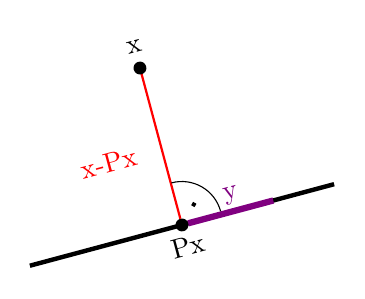
\begin{tikzpicture}[rotate=15,transform shape]
  \draw[ultra thick, draw=black] (0,0) -- (4,0) ;
  \node[red] (xPx) at (1.3,1) {x-Px};
  \node[draw,circle,fill,inner sep=1.5pt] (Px) at (2,0) {};
  \node[black] (PxText) at ($(Px.south) +(-0,-0.2)$) {Px};
  \node[violet] (Y) at (2.7,0.2) {y};
  \draw[thick,red] (Px)-- ++(90:2cm) ;
  \node [draw,circle,fill,inner sep =1.5pt,above=1.9cm of Px] (x) {};
  \node [black] at ($(x.north)+(0,0.2)$) {x};
  \node[draw,circle,fill,inner sep=0.5pt] (ra) at ([shift=(45:0.3cm)]Px) {};
  \draw[line width=0.8mm,violet] (Px) -- (3.2,0);
  \draw[] ([shift=(4.5:0.52cm)]Px) arc (0:90:0.51cm);
  \end{tikzpicture}
  \end{center}
\end{figure}



Now recall that $H:=\mathcal L^2(\Omega, \mathcal A, \P)$ (more precisely, their equivalence classes $L^2(\Omega, \mathcal A, \P)$, see Theorem \ref{Lp} and the discussion around) is a Hilbert space with $\langle X,Y\rangle=\E[XY]$. As a subspace we choose $G:=\mathcal L^2(\Omega, \mathcal F,\P)$ which is closed as limits of measurable maps do not loose the measurability.  We first check that $P: X\mapsto \E[X|\mathcal F]$ is a mapping from $H$ to $G$. The measurability is clear from the first property of conditional expectation, so we need to check the square-integrability. Jensen's inequality gives $\mathbb E[X|\cF]^2 \leq \mathbb E[X^2|\cF]$ a.s. so that monotonicity of expectations yields
		\begin{align*}
			\mathbb E\big[\mathbb E[X|\cF]^2\big] &\leq \mathbb E\big[\mathbb E[X^2|\cF]\big] = \mathbb E[X^2] < \infty.
		\end{align*}
	In order to prove the claimed minimisation property we proof the equivalent orthogonality property. This is easier as we can manipulate with linearity. Let $Y \in \cL^2(\Omega,\cF,\mathbb{P})$, so that $\mathbb E[\lvert XY \rvert] < \infty $ by Cauchy-Schwarz. Then we can use the properties for expectations and conditional expectations to deduce
		\begin{align*}
			\langle Y,X - \mathbb E[X|\cF]\rangle 			\overset{\text{lin., def.}}&{=} \mathbb E[YX] - \mathbb E[Y\mathbb E[X|\cF]] \\
			\overset{Y\,\mathcal F\text{-meas.}}&{=} \mathbb E[YX] - \mathbb E[\mathbb E[YX|\cF]] \\
	&=\mathbb E[YX] - \mathbb E[YX]\\
	&=0.
		\end{align*}
\end{proof}
We finish the abstract theory with an application to independence. Recall that two $\sigma$-algebras $\mathcal F_1, \mathcal F_2$ are called independent if all choices of pairs $A, B$ from the $\sigma$-algebras are independent: $\P(A\cap B)=\P(A)\P(B)$. Equivalently, all pairs random variables that are measurable with respect to the $\sigma$-algebras are independent random variables.
\begin{llemma}
\begin{prop}
	Two sub-$\sigma$-Algebras $\cF_1$ and $\cF_2$ of $\mathcal A$ are independent if and only if $\mathbb E[X\,|\,\cF_1] = \mathbb E[X]$ a.s. for all $\cF_2$-measurable $X \geq 0$
\end{prop}
\end{llemma}
\begin{proof}[Proof]
"$\Rightarrow$": Follows from Theorem \ref{cond_properties} (vii).\smallskip
	
"$\Leftarrow$": Taking $A\in \cF_2$ and $B\in \cF_1$ we need to show $\mathbb P(A\cap B)=\mathbb P(A)\mathbb P(B)$. All we use is the non-negative random variable $X=\mathbf 1_A$. Using elementary properties of the expectation and  Theorem \ref{cond_properties} (iv)
	\begin{align*}
	\mathbb{P}(A\cap B) &= \mathbb E[\mathbf 1_{A \cap B}] 
	= \mathbb E[\mathbb E[\mathbf 1_A \mathbf 1_B |\cF_1]] 
	\overset{B\in \cF_1}{=} \mathbb E[\mathbf 1_B \mathbb E[\mathbf 1_A |\cF_1]] 
	\overset{\text{ass.}}{=} \mathbb E[\mathbf 1_B \E[\mathbf 1_A]] = \mathbb{P}(B) \mathbb{P}(A).
	\end{align*}
\end{proof}

\begin{example}\label{so}
	Let $X_1,...,X_n$ iid random variables on $(\Omega, \mathcal A, \P)$ and $X=\sum_{k=1}^n X_k$. Then 
	\begin{align*}
		\E[X_k|X]=\frac X n\,\,\text{a.s.}\quad \text{and}\quad \E[X|X_1]=(n-1)\E[X_1]+X_1\,\,\text{a.s.}
	\end{align*}
	Before we proof the identity by checking the definition we intuitively derive the results. If we know nothing about the $X_k$ but the value of the sum then the best constant guess for each of the summands (using iid) is the value of the sum divided by $n$. The second is easier to guess. Fixing the value of $X_1$ the best constant guess of the sum is the expectation of the sum of $n-1$ copies plus the fixed values. Let us now check the claims rigorously. The second claim is just the linearity of conditional expectation combined with the elementary properties (iv) and (i). For the first claim first note that 
\begin{align}\label{ppp}
	\E[X_1|X]=...=\E[X_n|X]\quad \text{a.s.}
\end{align}	
	 Why? If $A\in \sigma(X)$, then we can write $\mathbf 1_A=h(X)=f(X_1,...,X_n)$ so that
	\begin{align*}
		\E[X_1\mathbf 1_A]=...=\E[X_n\mathbf 1_A],
	\end{align*}
	because the iid assumptions yields $\E[g(X_1,...,X_n)]=\E[g(X_{\sigma(1)},...,X_{\sigma(n)})]$ for all permutations $\sigma$. But then \eqref{ppp} follows from property (x) of conditional expectation. Now linearity used for the sum $X$ implies $\E[X_1|X]=...=\E[X_n|X]=\frac 1 n \E[X|X]=\frac 1 n X.$
\end{example}

%Let us recall that usual expectations were defined in an abstract way but have simple formulas for discrete and absolutely continuous random variables:
%\begin{align*}
%	\E[X]=\begin{cases}
%		\int_\R x\,\mathbb P_X(\dint x)&: \text{general formula}\\
%		\sum_{k=1}^N a_k p_k&: \text{discrete case}\\
%		\int_\R x\,f_X(x)\dint x&:\text{absolutely continuous case}
%	\end{cases}
%\end{align*}
%The situation is similar for conditional expectations. In nice situations there are simple formulas for the object defined through abstract axioms.  
%\begin{llemma}
%\begin{prop}\label{pjc}
%	Suppose $X,Y$ are integrable random variables on $(\Omega, \mathcal A, \mathbb P)$ with joint density $f$. Then
%	\begin{align}\label{cont1}
%		\E[X\,|\, Y]=\int_\R x \frac{f(x,Y)}{f_y(Y)}\mathbf 1_{f_y(Y)>0}\dint x\quad \text{a.s.},
%	\end{align}
%	where $f_y(y)=\int_\R f(x,y)\dint x$ is the density of $Y$.
%\end{prop}
%\end{llemma}
%\begin{proof}[Proof]
%	As always we need to check the defining properties of conditional expectation for the right-hand side. The measurability condition holds as 
%	\begin{align*}
%		z\mapsto \phi(z):=\int_\R x \frac{f(x,z)}{f_y(z)}\mathbf 1_{f_y(z)>0}\dint x
%	\end{align*}
%	is a measurable mapping (approximate the integral by a sum and use that limits of measurable functions are measurable), so that plugging-in $Y$ makes $\phi(Y)$ $\sigma(Y)$-measurable. To check the expectation property we show $\mathbb E[X\mathbf 1_A]=\E[\phi(Y)\mathbf 1_A]$ for all $A\in \sigma(Y)$. Since $\phi(Y)$ is exactly the right-hand side of \eqref{cont1} the claim will follow. The factorisation lemma yields a measurable function so that $\mathbf 1_A=g(Y)$. Hence,
%	\begin{align*}
%			\mathbb E[X \mathds 1_A] &=\mathbb E[Xg(Y)]\\
%			\overset{\ref{ber1}}&{=} \int_{\mathbb{R}^2} xg(y)f(x,y)\dint (x,y) \\
%			\overset{\text{Fub.}}&{=} \int_{\mathbb{R}} \Big( \int_{\mathbb{R}} xf(x,y)\dint x \Big) g(y)\dint y \\
%			\overset{f_y=0\Rightarrow f=0}&{=} \int_{\mathbb{R}} \Big( \int_{\mathbb{R}} xf(x,y)\mathbf 1_{f_y(y)>0}\dint x \Big) g(y)\dint y \\
%			&= \int_{\mathbb{R}}\Big(\int_{\mathbb{R}}  \frac{x f(x,y)}{f_y(y)}\mathbf 1_{f_y(y)>0}\dint x\Big)  f_y(y)g(y)\mathds 1_{f_y(y)\geq 0}\dint y \\
%			&= \int_{\mathbb{R}} \phi (y) f_y(y) g(y) \dint y \\
%			&= \mathbb E[\phi (Y)g(Y)] \\
%			&= \mathbb E[\phi (Y) \mathds 1_A].
%	\end{align*}
%	Hence, the claim follows.
%\end{proof}

%The discrete case has been discussed in detail at the end of Section \ref{sec:gentle}. For completeness let us summarise the situation in a proposition:
%\begin{llemma}
%\begin{prop}
%	Suppose $Y$ is a discrete random variable with values $a_1,...,a_N$. Then 
%	\begin{align*}
%		\E[X| Y]=\sum_{k=1}^N \E[X|Y=a_k] \mathbf 1_{Y=a_k}\quad \text{a.s.},
%	\end{align*}
%	where $\E[X | Y=a_k]=\frac{\E[X \mathbf 1_{Y=a_k}]}{\P(Y=a_k)}$ is the conditional expectation of $X$ given $\{Y=a_k\}$.
%\end{prop}
%\end{llemma}
%Comparing the two special cases above we see that the right hand sides take the form $h(Y)$ for an explicit function $h$. This is the measurable function $h$ from the factorisation lemma! In the discrete case $h$ is particularly simple, $h(y)=\E[X|Y=y]$ for the values $a_1,...,a_N$ of $Y$ and something else otherwise. We take this as a motivation to define $\E[X|Y=y]$ for general random variables.
%\begin{deff}
%	Suppose $X,Y$ are integrable random variables on $(\Omega, \mathcal A, \mathbb P)$ and $h$ a measurable function from the factorisation lemma so that $\E[X|Y]=h(Y)$ a.s.	Then we define
%	\begin{align*}
%		\E[X|Y=y]:=h(y)
%	\end{align*}
%	and call it the conditional expectation of $X$ given $Y=y$.
%\end{deff}
%There is an important warning to be made. If we function $h$ is modified on a set of zero measure for $\P_Y$ to get a function $\bar h$, then $\bar h(Y)$ is also a version of $\E[X|Y]$. But then we do not know if we should choose $h$ or $\bar h$ in the definition of $\E[X|Y=y]$. This reflects the fact that $\E[X|Y=y]$ is not well defined for a fixed value $y$ but only as a function of all $y$ and the function is only unique up to zero sets of $\P_Y$! One should keep the discrete case in mind where $\E[X|Y=y]$ can be defined to some (irrelevant) value if $Y=y$ does not happen.





\section{Conditional expectation for random variables}
The most important special case with many applications in statistics is $\E[X|Y]$, sometimes also more generally $\E[h(X,Y)|Y]$, the conditional expectation of an integrable random variable with respect to another random variable. Interestingly, we can use this conditional expectation to gain a much deeper understanding of random vectors than we have so far. Let us first recall from Stochastik 1 some definitions on pairs of random variables.
\begin{lstep}
If $(X,Y)$ is a random vector of two random variables $X$ and $Y$ then $\P_{(X,Y)}(A\times B)=\P(X\in A, Y\in B)$ was called the law of $(X,Y)$. The law is a probability measure on the product space $(\R\times \R, \mathcal B(\R)\otimes \mathcal B(\R))$ which is uniquely determined by the joint distribution function $F_{(X,Y)}(t_1,t_2)=\P_{(X,Y)}((-\infty,t_1)\times (-\infty,t_2))$. In analogy to the case of one random variable, expectations $\E[h(X,Y)]$ were defined by $\int_\Omega h(X,Y)\dint \P$ which, using the transformation formula and Fubini, equals $\int_\R \int_\R h(x,y)  \P_{(X,Y)}(\textrm d x,\textrm d y)$. The formula simplifies a lot for independent random variables for which the law $\P_{(X,Y)}=\P_X\otimes \P_Y$ is a product measure and we can integrate the two coordinates separately. An important technical point was that it suffices to define measures on $\mathcal B(\R)\otimes \mathcal B(\R)$ on rectangular sets $A\times B$ to obtain a measure on the entire $\sigma$-algebra, see the proof of Theorem \ref{EindVert}. The key words are Dynkin-systems for uniqueness and Carath\'eodory for the existence.
\end{lstep}
 In Stochastik 1 the structure of dependent random variables remained widely open, we only motivated dependence informally as "{}$X$ influences $Y$ or $Y$ influences $X$"{} and defined dependent as not being independent. In this section conditional expectation are used to understand properly the  dependence of random variables and to get a handy formula to computing conditional expectations.
\begin{ldef}
\begin{deff}
	Let $(R,\mathcal R)$ and $(S, \mathcal S)$ measurable spaces. Then a mapping $\kappa: R\times \mathcal S\to [0,\infty]$ is called a \textbf{Markov kernel} (or \textbf{transition kernel}) on $R\times \mathcal S$ if 
	\begin{enumerate}[label=(\roman*)]
		\item $y\mapsto \kappa(y,A)$ is $(\mathcal R, \mathcal B(\bar \R))$-measurable for all $A\in \mathcal S$,
		\item $A\mapsto \kappa(y,A)$ is a probability measure for all $y\in R$.
	\end{enumerate}	
\end{deff}
\end{ldef}
We think of a kernel to be a measure parametrised by a real parameter, such as the law of the exponential distribution which is parametrised by $\lambda$. The defining properties of a kernel are best understood through the next proposition. The definition of the integral needs the measurability of the integrand and the measure property of the left hand side needs the measure property of the kernels.
\begin{llemma}
\begin{prop}
	Suppose $Y$ is a random variable and $\kappa$ is a transition kernel on $\R\times \mathcal B(\R)$, then there is a another random variable $X$ such that the joint law of $X$ and $Y$ satisfies
	\begin{align}\label{joint}
		\P_{(X,Y)}(A\times B)=\int_B \kappa(y,A) \,\P_Y(\mathrm d y),\quad A,B\in\mathcal B(\R).
	\end{align}
\end{prop}
\end{llemma}
\begin{proof}[Proof]
	All we need to do is to use the right hand side as a definition of a probability measure $\mu$ on $\mathcal B(\R)\otimes \mathcal B(\R)$ through the distribution function
	\begin{align*}
		F(t_1,t_2):= \int_{(-\infty,t_2]} \kappa(y,(-\infty,t_1]) \P_Y(\mathrm dy)
	\end{align*}	
	for all $t_1,t_2\in\R.$
	\begin{luebung}
		Check the properties of a multivariabe distribution function using dominated convergence and linearity/monotonicity of integrals.		
	\end{luebung}
	 Then Theorem \ref{kan} gives us a pair $(X,Y)$ of random variables with distribution function $F$, hence, the joint law fulfills Equation \eqref{joint}.
\end{proof}

	\marginpar{\textcolor{red}{Lecture 3}}
\begin{lwarnhinweis}
	Kernels are not unique! If two kernels are only $\P_Y$-almost surely equal, then the integrals in \eqref{joint} are the same. 
\end{lwarnhinweis}
Laws $\P_{(X,Y)}$ on the product space defined through kernels are the natural generalisation of product measures $\P_X\otimes \P_Y$, the laws of independent random variables. Indeed, if $\kappa(y,\cdot)=\P_X$ is independent of $y$, then \eqref{joint} simplifies to 
		\begin{align*}
			\P_{(X,Y)}(A\times B)=\int_B \P_X(A)  \P_Y(\mathrm d y)=\P_X(A) \P_Y(B),
		\end{align*}	
	the formula describing independent random variables. The entire point of kernels is to understand better the concept of dependent random variables. A good probabilistic interpretation of random vectors $(X,Y)$ with distribution \eqref{joint} goes as two-stage experiment. First sample from $Y$ and given the value of $Y$ sample from $X$ which distribution depends on the value $y$ of $Y$.
	\begin{llemma}
	\begin{deff}
		We call two random variables $X$ and $Y$ a \textbf{two-stage experiment} with transition kernel $\kappa$ if $\P_{(X,Y)}$ can be written in the disintegration form of \eqref{joint}.
	\end{deff}
	\end{llemma}
		The wording transition kernel makes much more sense with the notion of two-stage experiments in mind as $\kappa$ describes the transition from the first stage to the second stage of the experiment.\smallskip
	
	Here is an instructive example. First choose uniformly $p$ from $[0,1]$ and then toss a coin with probability of success $p$. This simple two-stage experiment is modelled through
	\begin{align*}
		\P_Y\sim \mathcal U([0,1]),\quad \kappa(p,A )= \big(p\delta_{\{1\}}(A)+(1-p)\delta_{\{0\}}(A)\big) \mathbf 1_{[0,1]}(p).
	\end{align*}
	The two properties of a kernel are obviously fulfilled in this example.\smallskip

		
	% gives $\P_Y\sim \mathcal U([0,1])$ and $\kappa(p,\cdot)\sim p\delta_{\{1\}}+(1-p)\delta_{\{0\}}$.\smallskip

%As usual the discrete and absolutely continuous cases are more explicit.
%\begin{example}\label{ExA}
%	\begin{enumerate}[label=(\roman*)]
%			\item If $p_1,...,p_N\geq 0$ sum up to $1$ and $\P_1,...,\P_N$ are distributions of $N$ random variables, then
%		\begin{align*}
%			\kappa(y,A)=\sum_{k=1}^N \P_k(A) \mathbf 1_{y=a_k}
%		\end{align*}
%		is a kernel. The corresponding $\P_{(X,Y)}$ is the experiment in which a discrete random variable $Y$ determines which of $N$ experiments $X_k$ is executed next.		
%		\item If $f$ is a joint density function (jointly measurable, non-negative with integral $1$), then
%		\begin{align}\label{dens}
%			\kappa(y,A):=\int_A \frac{f(x,y)}{f_y(y)}\mathbf 1_{f_y(y)>0}\dint x
%		\end{align}
%		is a kernel, where $f_y=\int_\R f(x,y)\dint y$.
%		\item Every probability measures $\P_X$ determines a trivial kernel $\kappa(y,A):=\P_X(A)$ which leads us to independent random variables as we know their distribution is the product measure:
%		\begin{align*}
%			\P_{(X,Y)}(A\times B)=\int_B \P_X(A)  \P_Y(\mathrm y)=\P_X(A) \P_Y(B).
%		\end{align*}	
%	\end{enumerate}
%\end{example}
It might be surprising, but \textbf{every} pair of random variables can be seen as a two-stage experiment!
\begin{lsuperwichtigersatz}
\begin{theorem}[Disintegration of $(X,Y)$ into $Y$ and a kernel]\label{kernel}
	Suppose $X$ and $Y$ are random variables on $(\Omega, \mathcal A, \P)$, then there is a kernel $\kappa$ on $\R\times \mathcal B(\R)$ such that
	\begin{align}\label{main2}
		\P_{(X,Y)}(A\times B)=\int_B \kappa(y,A) \,\P_Y(\mathrm d y),\quad A, B\in \mathcal B(\R).
	\end{align}
	The kernel is unique up to null-sets of $\P_Y$.
\end{theorem}
\end{lsuperwichtigersatz}
The formula appearing in the theorem is called a disintegration (\glq Zerlegegung\grq), meaning the inverse of producing one measure from several measures as seen in Proposition \ref{joint}. Again, keep in mind that $\kappa$ is not unique! Changing $\kappa$ on zero-sets of $Y$ gives other disintegrations. 
\begin{proof}[Proof]
	\textbf{Uniqueness:}
	Suppose there are two kernels $\kappa, \bar \kappa$. Setting $A=(-\infty,t]$ yields
	\begin{align*}
		\int_B \kappa(y,(-\infty,t]) \, \P_Y(\mathrm d y)=\int_B \bar \kappa(y,(-\infty,t]) \, \P_Y(\mathrm dy),\quad t\in\Q, B\in \mathcal B(\R).
	\end{align*}
	This implies that there are sets $\mathcal M_t$ with $\P_Y(\mathcal M_t)=1$ so that $\kappa(y,(-\infty,t])=\bar \kappa(y,(-\infty,t])$ for all $z\in \mathcal M_t$. Defining $\mathcal M:=\cap_{t\in \Q} \mathcal M_t$ yields equality of $\kappa(y,\cdot )$ and $\bar \kappa(y,\cdot )$ on an $\cap$-stable generator of $\mathcal B(\R)$ for all $y\in \mathcal M$. Since equality on an $\cap$-stable generator implies equality of measures (see Theorem \ref{Dynkin-Folgerung}) we obtain equality $\kappa(y,\cdot)=\bar \kappa(y,\cdot)$ for all $y\in \mathcal M$. Since $\mathcal M$ is the intersection of countably many events of probability $1$ the claim follows.\smallskip
	
		\textbf{Existence:}
	For every $r\in \Q$ let $g_{r}$ the measurable mappings from the factorisation lemma so that
	\begin{align*}
		g_{r}(Y):=\E[\mathbf 1_{(-\infty,r]}(X)|Y]\quad \text{a.s.}
	\end{align*}
	From the monotonicity of conditional expectations (countably many!) we deduce
	\begin{align*}
		\P(g_r(Y)\leq g_s(Y)\,\,\forall r\leq s)=1.
	\end{align*}
	In other words, the set $E_1:=\{y\in \R: g_r(y)\leq g_s(y) \,\,\forall r\leq s\}$ has measure $1$ under $\P_Y$. Similarly, using DCT for conditional expectations, the sets $E_2:=\{y\in \R: \inf_{r\in\Q} g_r(y)=0\}$ and $E_3:=\{y\in \R: \sup_{r\in\Q} g_r(y)=1\}$ have measure $1$ under $\P_Y$. Now define $$E:=E_1\cap E_2\cap E_3$$ which again has measure $1$ under $\P_Y$. What does this mean? For all $y\in E$ the mapping
	\begin{align*}
		r\mapsto g_r(y), \quad r\in \Q,
	\end{align*}
	is increasing and has the limits of a cumulative distribution function (CDF). Now we extend this to a family of CDFs. First choose the CDF $\mathbf 1_{[0,\infty)}$ and define
	\begin{align*}
		F_y(t):=\begin{cases}
			\inf\{g_r(y): r>t, r\in\Q \}&: y\in E\\
			\mathbf 1_{[0,\infty)}(t)&:y\notin E
		\end{cases},\quad t\in\R.
	\end{align*}
	We could have chosen any other CDF instead of $\mathbf 1_{[0,\infty)}$ but this particular choice leads to the simple form $\kappa(y,A)=0$ on the $\P_Y$-zero set in the formulas below. Now, for every $y\in \R$ the mapping $t\mapsto F_y(t)$ is increasing, with limits $0$ and $1$ and $-\infty$ and $+\infty$, and right-continuous. Writing down carefully these arguments requires a bit tedious analysis that does not provide deeper understanding, we prefer to skip them. Hence, the family $(F_y)_{y\in\R}$ is a family of CDFs. Additionally, for fixed $t\in \R$, the mapping $t\mapsto F_y(t)$ is measurable as it can be written as
	\begin{align*}
		y\mapsto F_y(t)= \underbrace{\mathbf 1_{[0,\infty)}(t) \mathbf 1_{E^C}(y)}_{\text{measurable}}+ \underbrace{\mathbf 1_{E}(y)}_{\text{measurable}}\underbrace{\inf\{g_r(y):t\leq r, r\in\Q \}}_{\text{measurable}},
	\end{align*}
	as a countable infimum of measurable functions is measurable. Now we are in a position to define the kernel. For every $y\in\R$ fixed we use the CDFs $F_y$ to define the corresponding probability measure $\kappa(y,\cdot)$ as usually (compare Theorem \ref{EindVert}):
	\begin{align*}
		\kappa(y,(a,b]):=F_y(b)-F_y(a),\quad a<b.
	\end{align*}
	It is clear from this construction that $A\mapsto \kappa (y,A)$ are probability measures for all $y\in\R$. To prove that $y\mapsto \kappa(y,A)$ is measurable we use the trick of good sets (compare for instance the proof of Theorem \ref{Dynkin-Folgerung}). Define
	\begin{align*}
		\mathcal M:=\big\{A\in \mathcal A\,|\, y\mapsto \kappa(y,A)\text{ is measurable}\big\}.
	\end{align*}
	Then $\mathcal M$ contains an $\cap$-stable generator of $\mathcal B(\R)$, namely the set $\mathcal E=\{(a,b]:a\leq b\}$, because $y\mapsto \kappa(y,(a,b])=F_y(b)-F_y(a)$ is measurable as a difference of two measurable functions. Additionally, $\mathcal M$-is also a Dynkin-system. The complement property holds as $y\mapsto \kappa(y,A^C)=1-\kappa(y,A)$ is measurable as a difference of two measurable functions. Now let $A_1,...$ be disjoint sets from $\mathcal M$. Then we see that
	\begin{align*}
		y\mapsto \kappa\Big(y,\bigcupdot_{k=1}^\infty A_k\Big)=\sum_{k=1}^\infty \kappa(y,A_k)=\lim_{n\to\infty}\sum_{k=1}^n \kappa(y,A_k)
	\end{align*}
	is measurable as a limit of measurable maps. Hence, $\mathcal M$ is closed under disjoint unions. Now we can use the "{}trick of good sets"{}:
	\begin{align*}
		\mathcal A=\sigma(\mathcal E)\overset{\ref{Hauptsatz}}{=}d(\mathcal E)\subseteq d(\mathcal M) \subseteq \mathcal A
	\end{align*}
	which implies $\mathcal M=\mathcal A$. In other words, $y\mapsto \kappa(y,A)$ is measurable for all $A\in \mathcal A$. \smallskip
	
	To finish the proof we only need to check the identity \eqref{main2} on some $\cap$-stable generator of $\mathcal B(\R)\otimes \mathcal B(\R)$. We use the set of infinite rectangles $(-\infty,t]\times (-\infty,s]$ with rational end-points:
	\begin{align*}
	\int_{(-\infty,s]} \kappa (y,(-\infty,t]) \P_Y(\mathrm dy)
	&=\int_\R \kappa (y,(-\infty,t])  \mathbf 1_{(-\infty,s]}(y)  \P_Y(\mathrm d y)\\
	&=\E\left[ \kappa (Y,(-\infty,t])  \mathbf 1_{(-\infty,s]}(Y) \right]\\
	\overset{\text{def. }\kappa}&{=}\E\left[ \E[\mathbf 1_{(-\infty,t]} (X)|Y]\mathbf 1_{(-\infty,s]}(Y)\right]\\
	\overset{\text{meas.}}&{=}\E\left[ \E[\mathbf 1_{(-\infty,t]} (X)\mathbf 1_{(-\infty,s]}(Y)|Y]\right]\\
		\overset{\text{$\E$ of cond. exp.}}&= \E[\mathbf 1_{(-\infty,t]} (X)\mathbf 1_{(-\infty,s]}(Y)]\\
		&=\P(X\leq t, Y\leq s)\\
	&=\P_{(X,Y)}((-\infty,t]\times {(-\infty,s]}).
\end{align*}
\end{proof}
There are several situations in which the kernels $\kappa$ can be guessed and have a nice form. The most important examples are absolutely continuous random vectores: 
	\begin{lwarnhinweis}
	If $X,Y$ have a joint density $f$, then 
	\begin{align*}
		\kappa(y,A)=\int_A \frac{f(x,y)}{f_y(y)}\mathbf 1_{f_y(y)>0}\dint x,\quad y\in\R, A\in \mathcal B(\R),
	\end{align*}
	where $f_y(y)=\int_\R f(x,y)\dint x$.
	\end{lwarnhinweis}
	The formula follows directly from the standard calculation rules of probability theory:
	\begin{align*}
		\P_{(X,Y)}(A\times B)=\int_{A\times B} f(x,y)\dint (x,y)&=\int_B\Big( \int_A \frac{f(x,y)}{f_y(y)}\mathbf 1_{f_y(y)>0} \dint x\Big)f_y(y)\dint y\\
		&=\int_B \kappa(y,A)  \P_Y(\mathrm dy).
	\end{align*}
	\begin{lwarnhinweis}
	If $Y$ is discrete with values $a_1,...,a_N$, then
	\begin{align*}
		\kappa(y,A)&=\sum_{k=1}^N\P(X\in A|Y=y)\mathbf 1_{\{a_k\}}(y)\\
		&=\begin{cases}
		\P(X\in A|Y=a_k)&: y=a_k\\			
		0&: \text{otherwise}
		\end{cases} ,\quad y\in\R, A\in \mathcal B(\R).
	\end{align*}
	\end{lwarnhinweis}
	The formula is a direct consequence of the formula of total probability:
	\begin{align*}
		\P_{(X,Y)}(A\times B)&=\P(X\in A,Y\in B)\\
		&=\sum_{a_k\in B} \P(X\in A|Y=a_k)\P(Y=a_k) \\
		\overset{\ref{IntDiskr}}&{=}\int_\R \kappa(y,A)\, \P_Y(\mathrm d y).
	\end{align*}
	%lkjsdffd
With the powerful disintegration theorem in hands we can understand how to compute with conditional expectations for random variables. Keeping in mind the explicit formulas in special cases above, the theorem allows us to perform many explicit computations.
\begin{lsatz}
\begin{theorem}\label{formeln}
	Suppose $X$ and $Y$ are random variables, $X$ integrable, and $h:\R^2\to\R$ is measurable, then
	\begin{enumerate}[label=(\roman*)]
		\item $\E[h(X,Y)|Y]=\int_\R  h(x,Y)\, \kappa(Y,\mathrm dx)$ a.s.,
		\item	$\E[X|Y]=\int_\R x  \, \kappa(Y,\mathrm{d} x)$ a.s.,
	\end{enumerate}
	where $\kappa$ is the kernel from Theorem \ref{kernel}
\end{theorem}
\end{lsatz}
\begin{proof}[Proof]
	We only need to prove the first claim, the second follows by choosing $h(x,y)=x$. As usually we check the two defining properties of conditional expectation. The righthand side can be written as $\phi(Y)$ with
	\begin{align*}
		\phi(z)=\int_\R h(x,z)\, \kappa(z,\mathrm{d} x). 
	\end{align*}
	As $\phi$ is measurable (approximate the integral by sums) we immediately get that $\phi(Y)$ is $\sigma(Y)$-measurable. For the expectation property fix some $A\in \sigma(Y)$. According to the factorisation lemma there is a Borel map $g$ so that $\mathbf 1_A=g(Y)$. Now we compute:
	\begin{align*}
		\E[\mathbf 1_A \phi(Y)]
		&=\E\Big[g(Y)\int_\R  h(x,Y) \,\kappa(Y,\mathrm dx)\Big]\\
		&=\E\Big[\int_\R g(Y) h(x,Y) \,\kappa(Y,\mathrm dx)\Big]\\
		&=\int_\R \int_\R g(y) h(x,y) \, \kappa(y,\mathrm dx)\,\P_Y(dy)\\
		\overset{(*)}&{=}\int_\R \int_\R g(y) h(x,y) \P_{(X,Y)}(\mathrm dx,\mathrm dy)\\
		&=\E[g(Y) h(X,Y)]\\
		&=\E[\mathbf 1_A h(X,Y)].
	\end{align*}	
	The equality $(*)$ needs some clarification. For indicator functions $f=\mathbf 1_{A\times B}$ of rectangle sets the equality 
	\begin{align}\label{tes}
		\int_\R \int_\R f(x,y)\,\kappa(y,\mathrm dx)\,\P_Y(dy)= \int_\R \int_\R f(x,y)\, \P_{(X,Y)}(\mathrm dx,\mathrm dy)
	\end{align}
	holds by the definition of the kernel. Now define $\mathcal M:=\{M\in \mathcal B(\R^2): \eqref{tes} \text{ holds for } f=\mathbf 1_M\}$. Using that indicators over disjoint unions are sums over indicators and monotone convergence we see that $\mathcal M$ is a Dynkin-system containing the $\cap$-stable generator $\mathcal E:=\{A\times B: A,B\in \mathcal B(\R)\}$ of the Borel-$\sigma$-algebra. But then, as usually 
	\begin{align*}
		\mathcal B(\R^2)=\sigma(\mathcal E)\overset{\ref{Hauptsatz}}{=}d(\mathcal E)\subseteq d(\mathcal M)=\mathcal M\subseteq \mathcal B(\R^2).
	\end{align*}
	Hence, Equality \eqref{tes} holds for all indicators over $M\in \mathcal B(\R^2)$. But then it holds for all simple functions, with monotone convergence for all non-negative measurable functions and by splitting $f=f^+-f^-$ for all measurable functions. Finally, we apply \eqref{tes} with the function $f(x,y)=g(y)h(x,y)$.
\end{proof}
The theorem can be used for abstract considerations but also for explicit computations. To perform explicit computations the kernel $\kappa$ needs to be known. We collected several examples of kernels above, they cover most of the relevant situations in applications. Here are some examples to try:
\begin{luebung}
	\begin{enumerate}[label=(\roman*)]
			\item $\E[(Y-X)^+|X]$, where $X,Y$ are independent uniform random variables on $[0,1]$.
				\item $\E[X|X+Y]$, where $X,Y$ are independent Poisson random variables with parameters $\lambda$ and $\mu$ respectively.
		\item $\E[X|Y]$, where $X,Y$ has a joint density
		\begin{equation*}
			f(x,y)=4y(x-y)e^{-(x+y)} \mathbf 1_{0<y<x}.
		\end{equation*}
	%	\item $X,Y,Z$ are i.i.d. standard Gaussian random variables. $U=2X-Y-Z$, $V= 3X+Y-4Z$, calculate $\Exp{V|U}$.
	\end{enumerate}
\end{luebung}
The kernel $\kappa$ can be used to give a rigorous discussion of regular conditional distributions, the distributions behind the conditional expectations. The wording regular refers to the measurability in $y$ of the kernel.
\begin{llemma}
\begin{deff}[Regular conditional distributions]
	Let $X$ and $Y$ be random variables and $A\in \mathcal B(\R)$. If $\kappa$ is the kernel from Theorem \ref{kernel}, then we define $$\P(X\in A|Y)=\kappa(Y,A),\quad A\in \mathcal B(\R),$$
	and 
	\begin{align*}
			\P(X\in A|Y=y):=\kappa(y,A),\quad y\in \R, A\in \mathcal B(\R).
	\end{align*}

\end{deff}
\end{llemma}

	Recall that kernels are not unique as they can differ on zero sets of $\P_Y$. Hence, also $\P(X\in A|Y=y)$ is only well-defined as a function in $y$ up to null-sets of $\P_Y$. For the probabilistic intuition this perfectly makes sense. If $Y$ does not take the value $y$ why should we care about $\P(X\in A|Y=y)$?\smallskip


It is always instructive to check some examples. Use the discrete and absolutely formulas for $\kappa$ to compute the following conditional laws!
\begin{luebung}
\begin{enumerate}[label=(\roman*)]
\item Let $Z_1,Z_2$ be independent Poisson-distributed random variables with parameter $\lambda_1,\lambda_2 > 0$. Check that \[ \mathbb{P}\big(Z_1 = k \,\big|\, Z_1+Z_2 = n \big) = b_{n,p}(k),\quad k=0,1,...,\]  with $b_{n,p}(k)\sim \mathrm{Bin}(n,p)$ and $p=\frac{\lambda_1}{\lambda_1+\lambda_2}$.
\item What is  \[\mathbb{P}\big(Z_1\in \cdot \, | \, Z_1+Z_2 = x \big) \] if $Z_1$ and $Z_2$ are independent standard Gaussians? Define $X=Z_1$, $Y=Z_1+Z_2$, find $f_{x,y}$ and then compute with the formulas from above. There is also a more clever way to avoid computations somewhere hidden in these notes!
\end{enumerate}
\end{luebung}


Let us compare the definition with Theorem \ref{formeln} in the special case $h(x,y)=\mathbf 1_A(y)$. Then we see immediately the connection
\begin{align*}
	\E[\mathbf 1_A(X)|Y]=\kappa(Y,A)=\P(X\in A|Y)\quad \text{a.s.},
\end{align*}
which is exactly the classical connection $\E[\mathbf 1_A(X)]=\P(X\in A)$ between expectations and probabilities. Hence, the notion $\P(X\in A|Y)$ makes a lot of sense. There are other ways of construction $\P(X\in A|Y)$ more directly using the conditional expectation. One could for instance define $\P(X\in A|Y):=\E[\mathbf 1_A(X)|Y]$ but quickly runs into problems with zero sets that depend on $A$. Similar to the proof of Theorem \ref{kernel} the issue is resolved by defining the measures $\P(X\in (a,b]|Y)$ for rational end-points combined with a suitable extension to the reals. We do this in the next section to define $\P(X\in A|\mathcal F)$ for general $\sigma$-algebras.\smallskip

Due to the definitions through the kernel the function $y\mapsto \P(X\in A|Y=y)$ is the measurable mapping from the factorisation lemma that satisfies $h(Y)=\P(X\in A|Y)$. It is common practice to use this connection as an abstract definition of $\P(X\in A|Y=y)$. We prefer the construction through disintegration as the disintegration formula with $B=\R$ directly translates into the meaningful formula
	\begin{align*}
		\P(X\in A)=\int_\R \P(X\in A|Y=y) \P_Y(\mathrm dy),\quad A\in \mathcal B(\R),
	\end{align*}
	a formula that we understand very well in the discrete setting through the formula of total probabilities (recall Theorem \ref{formelnp}):
	\begin{align*}
		\P(X\in A)=\sum_{k=1}^N \P(X\in A|Y=a_k) \P(Y=a_k).
	\end{align*}
It also makes sense to replace the kernel in Theorem \ref{formeln} with the newly defined conditional probability to get a more intuitive feeling for the formulae:
\begin{align*}
	\E[h(X,Y)|Y]&=\int_\R h(x,Y)\, \P(X\in \mathrm dx|Y)\quad \text{a.s.}\\
	\E[X|Y]&=\int_\R x\, \P(X\in \mathrm dx|Y)\quad \text{a.s.}
\end{align*}


Just as $\P(X\in A|Y)$ is related through integration to $\E[h(X,Y)|Y]$ we can ask if $\P(X\in A|Y=y)$ is related to an object $\E[h(X,Y)|Y=y]$.  Indeed, this is the case in exactly the way we have seen before.





\begin{lsatz}
\begin{theorem}
	Suppose $X$ and $Y$ are random variables, $X$ integrable, and $h:\R^2\to\R$ is measurable, then
	\begin{enumerate}[label=(\roman*)]
		\item $\E[h(X,Y)|Y=y]:=\int_\R h(x,y) \, \P(X\in \mathrm dx|Y=y)$,
			\item $\E[X|Y=y]:=\int_\R x \, \P(X\in \mathrm dx|Y=y)$
	\end{enumerate}
	are the measurable functions from the factorisation lemma that turn $Y$ into $\E[h(X,Y)|Y]$ and $\E[X|Y]$.
\end{theorem}
\end{lsatz}
\begin{proof}[Proof]
	The right hand sides are measurable functions in $y$ and if we plug-in $Y$ then we obtain the conditional expectations by Theorem \ref{formeln}.
\end{proof}



		We have defined rigorously a couple of objects: $\E[X|Y]$, $\E[X|Y=y]$, $\P(X\in A|Y)$, and $\P(X\in A|Y=y)$ that are connected through integration and the factorisation lemma. Everything was based on the "{}most fine"{} object $\kappa(y,\cdot)$ from which we could reconstruct in a compact way all objects that relate to $X$ and $Y$. Explicit formulas in the most important special case allow explicit computations with conditional expectations and probabilities. The following diagram should give an overview over the relations. 
%\vspace{-2mm}
%	\begin{figure}[h]
%	\begin{center}
%		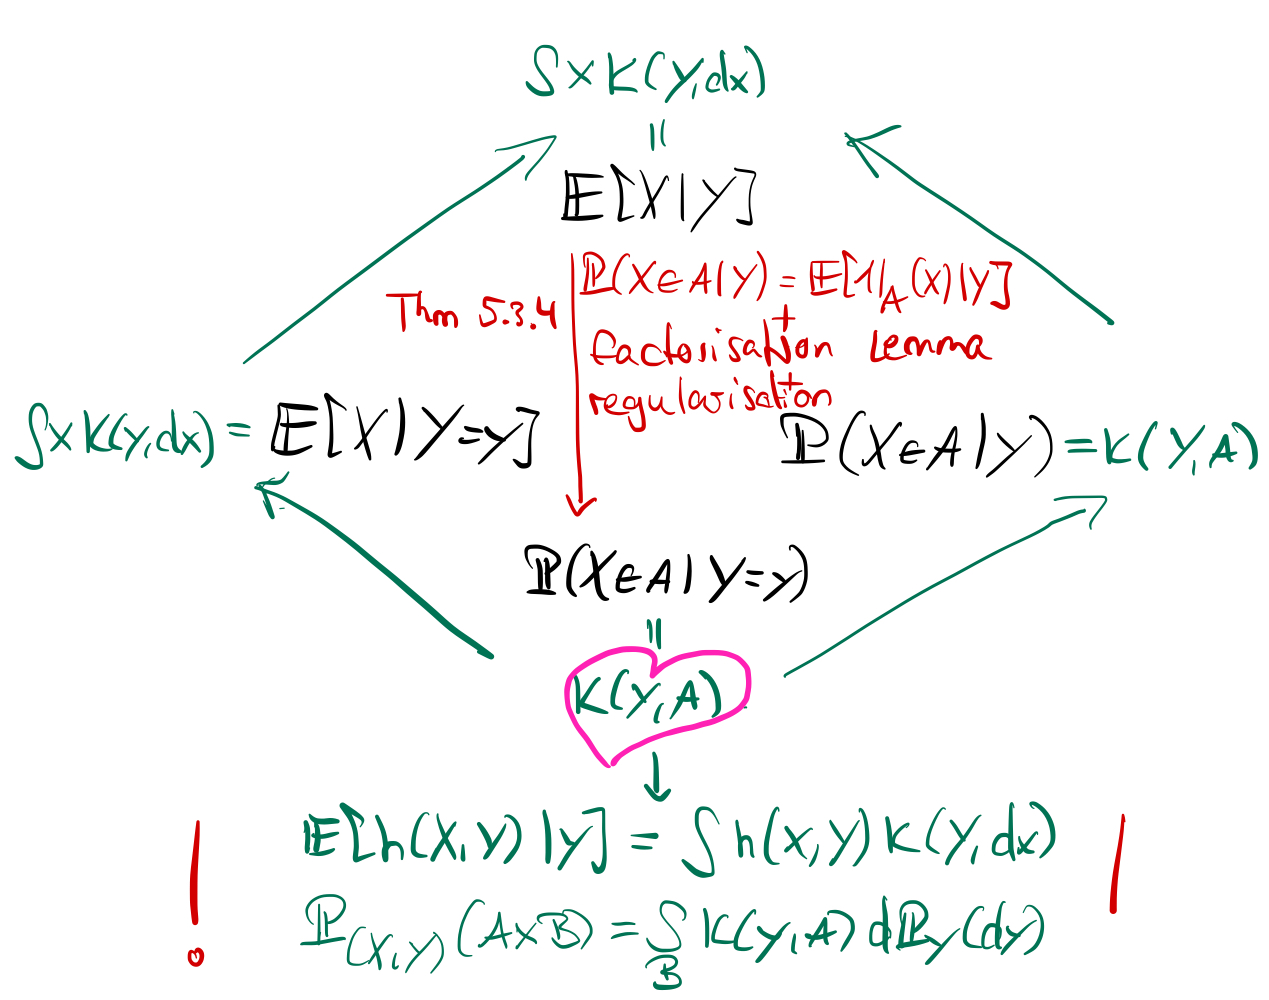
\includegraphics[scale=0.19]{CE9.jpeg}		
%	\end{center}
%		\vspace{-0.3cm}
%	\caption*{The logic behind the disintegration kernel and conditional expectation}
%\end{figure}

\begin{figure}[h]
\begin{center}
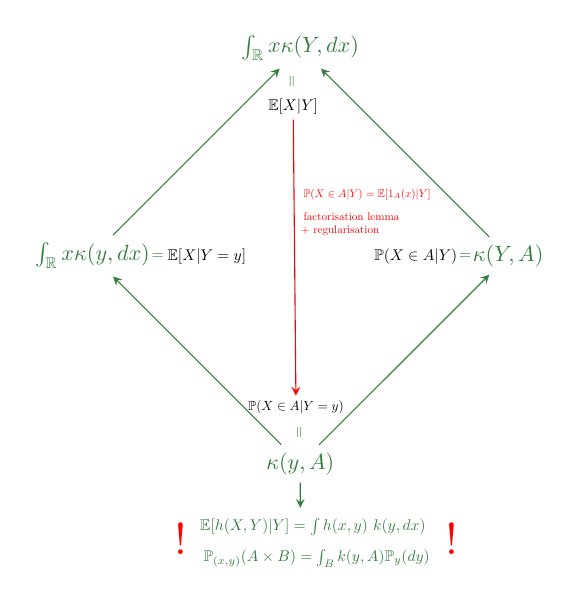
\begin{tikzpicture}[scale=0.8,transform shape]
  \tikzmath{\x = 3.3;}
  \node[darkgreen] (E1) at (0,\x) {$\int_{\mathbb{R}} x \kappa(Y,dx)$} ;
  \node[darkgreen,rotate=90,scale=0.7] (eq1) at ($(E1.south)+(0,-0.2)$) {}; 
  \node[darkgreen,rotate=90,scale=0.7] (eq) at ($(E1.south)+(-0.12,-0.2)$) {$=$}; 
  \node[black,scale=0.7] (equation1) at ($(eq1.south) +(-0.2,-0.4)$) {$\mathbb{E}[X|Y]$};

  \node[darkgreen] (E2) at (\x,0) {$\kappa(Y,A)$} ;
  \node[darkgreen,scale=0.7] (eq2) at ($(E2.west)+(0,-.02)$) {$=$}; 
  \node[black,scale=0.7] (equation2) at ($(eq2.west) +(-0.6,0)$) {$\mathbb{P}(X \in A|Y)$};

  \node[darkgreen] (E3) at (0,-\x) {$ \kappa(y,A)$} ;
  \node[darkgreen,rotate=90,scale=0.7] (eq3) at ($(E3.north)+(0,0.2)$) {$=$}; 
  \node[black,scale=0.6] (equation3) at ($(eq3.south) +(-0.2,0.4)$) {$\mathbb{P}(X \in A | Y=y)$};

  \node[darkgreen] (E4) at (-\x,0) {$\int_{\mathbb{R}}x \kappa(y,dx)$} ;
  \node[darkgreen,scale=0.7] (eq4) at ($(E4.east)+(0,-.02)$) {$=$}; 
  \node[black,scale=0.7] (equation4) at ($(eq4.east) +(0.6,0)$) {$\mathbb{E}[X|Y=y]$};

  \draw[-stealth,draw=darkgreen] (E4)--(E1);
  \draw[-stealth,draw=darkgreen] (E2)--(E1);
  \draw[-stealth,draw=darkgreen] (E3)--(E2);
  \draw[-stealth,draw=darkgreen] (E3)--(E4);
  
  \draw[-stealth,draw=red] (equation1) -- (equation3);
  \node[red,scale=0.6] (theorem1) at ($(eq1.south) +(-1.,-1.8)$) {};
  \node[red,scale=0.5] (theoremEq) at ($(theorem1.east) +(1.9,-0)$) {$\mathbb{P}(X\in A | Y) = \mathbb{E}[\mathbbm{1}_A(x)|Y]$};
  \node[red,scale=0.5] (theoremTxt1) at ($(theoremEq.south)+(-0.25,-0.2)$) {factorisation lemma};
  \node[red,scale=0.5] (theoremTxt2) at ($(theoremTxt1.south) +(-0.18,-0.1)$) {+ regularisation};

  \draw[-stealth,draw=darkgreen] (E3) -- (0,-4);
  \node[darkgreen,scale=0.7] (equation5) at (0.2,-4.3) {$\mathbb{E}[h(X,Y)|Y] = \int h(x,y)\ k(y,dx)$};
  \node[darkgreen,scale=0.7] (equation6) at (0.26,-4.8) {$\mathbb{P}_{(x,y)}(A\times B) = \int_B k(y,A)\mathbb{P}_y(dy)$};
  \node[red,scale=2] (!) at (-1.9,-4.5)  {!}; 
  \node[red,scale=2] (!) at (2.4,-4.5)  {!}; 
\end{tikzpicture}
	\caption*{The logic behind the disintegration kernel and conditional expectation}
\end{center}
\end{figure}
We finish the section with a discussion on conditioning on zero sets.	A bit of care is needed about the interpretation of $\P(X\in A|Y=y)$ as typically the event $\{Y=y\}$ has probability zero. One can easily get confused about the notation as the elementary conditional probability $\P(A|B)=\frac{\P(A\cap B)}{\P(B)}$ is not defined for null-sets $B$. The point is that we did not use the elementary definition of conditional probability. Instead, we constructed in some obscure way a mapping $y\mapsto \P(X\in A|Y=y)$ that satisfies a general total probability rule 
	\begin{align*}
			\P(X\in A)=\int_\R \P(X\in A|Y=y)\, \P_Y(\mathrm d y),\quad A\in \mathcal B(\R).
	\end{align*}
	In general there is no reason to expect any relation to elementary conditioned probabilities. Nonetheless, there are two situation in which the definition $\P(X\in A|Y=y)=\kappa(y,A)$ coincides with elementary conditioning and that's why we abuse the notation of conditional probability.\smallskip
	
		 If $Y$ is discrete, then the above formulas give
			\begin{align*}
				\P(X\in A|Y=y)=\begin{cases} 
								\P(X\in A|Y=a_k) &: y=a_k\\
								0&:\text{otherwise}
							\end{cases}
			\end{align*}
		with elementary conditional probability on the right hand side.\smallskip			
			
		 If $X$ and $Y$ are jointly absolutely continuous with density $f>0$ there is another way to define $\P(X\in A|Y=y)$ through a limiting procedure. The result is exactly the same:
			\begin{align*}
	\P(X\in A|Y=y)&:=\lim_{\varepsilon \to 0}\P(X\in A|Y\in (y-\varepsilon,y+\varepsilon))\\
	&=\lim_{\varepsilon\to 0} \frac{\int_{y-\varepsilon}^{y+\varepsilon} \int_A f(x,y)\dint x\,dy }{\int_{y-\varepsilon}^{y+\varepsilon} f_y(y)\dint x}\\
	\overset{\text{l'Hospital}}&{=} \frac{\int_A f(x,y)\dint x}{f_y(y)}=\kappa(y,A),
\end{align*}
with the kernel for absolutely continuous random vectors.




\section{General regular conditional distributions}
	\marginpar{\textcolor{red}{Not part of\\ the course}}

We finish the discussion of conditional expectation with a generalisation of Theorem \ref{formeln} towards conditional expectations on a general $\sigma$-algebra $\mathcal F$. We want to provide a computation rule
\begin{align}\label{integrall}
	\E[h(X)|\mathcal F]=\int_\R h(x) \,\P(X\in \dint x|\mathcal F)\quad \text{a.s.}
\end{align}	
 for all measurable $h$. For $\mathcal F=\sigma(Y)$ we proved such a formula using the "{}random"{} measures $\P(X\in \mathrm d x|Y)=\kappa(Y,\mathrm dx)$. The general setting does not provide a kernel $\P(X\in A|Y=y)=\kappa(y,A)$ to work with but still allows us to construct a "{}random"{} measure  satisfying \eqref{integrall}
 
% 
 %The answer is yes, but this is far from obvious. Let's try to see where the problems come from by looking at classical expectations. Suppose we know $\E[h(X)]$ for enough measurable functions, say all indicators. Then we could recover the law of $X$ on $\mathcal B(\R)$ via $\P_X(B)=\P(X\in B)=\E[\mathbf 1_B(X)]$ and from this derive the formula $\E[h(X)]=\int_\R h(x) \P_X(\dint x)$ via monotone convergence. Suppose we did the same for the conditional expectation and define $\P_{X|\mathcal F}(B):=\E[\mathbf 1_B(X)|\mathcal F]$. Note that those are random variables! Immediately we will run into trouble. The problem is that all those conditional expectations $\E[\mathbf 1_B(X)|\mathcal F]$ are only defined up to nullsets. Since we have uncountably many Borel-sets the (random) measure $B\mapsto \P_{X|\mathcal F}(B)$ would be defined only up to an uncountable union of nullsets and this could be anything. We can work our way around this by choosing versions of the conditional expectation which are all defined on the same probability space. For this we will use the separability of $\R$, i.e. with $\Q$ there is a countable dense subset, so that we only need to define the measure on intervals with rational boundary. Since countable unions of nullsets are nullsets,
%	\begin{align*}
%		0 \leq \mu \left( \bigcup\limits_{k=1}^{\infty}N_k \right) \leq \sum \limits_{k=1}^{\infty} \mu (N_k) = \sum \limits_{k=1}^{\infty} 0 = 0,
%	\end{align*}
%	no problem will occur. If we can carry this out we will call this (random) measures $(\omega, B)\mapsto \P_{X|\mathcal F}(B)(\omega)$ the conditional distribution of $X$ given $\mathcal F$. To do anything interesting (like integration) with such measures we should also find a version which is measurable in $\omega$. If we can achieve this we will speak of a regular conditional distribution of $X$ given $\mathcal F$. \smallskip
		
%	As objects of that kind appear in many fields of probability we should give it a name:
\begin{ldef}
\begin{deff}
	Suppose $(\Omega, \mathcal A, \P)$ is a probability space. A Markov kernel $\mu$ on $\Omega\times \mathcal B(\R)$ is called a \textbf{random measure}.
\end{deff}
\end{ldef}
The simplest example of a random measure already appeared in the previous section. If $\kappa$ is a kernel and $Y$ is a random variable, then $\kappa(Y,\cdot)$ is a random measure. The measure property is clear, the measurability follows as the concatenation of $Y$ and $\kappa$ is measurable again.\smallskip

Random measures can be found at very different places in statistics and probability theory under different names. For conditional expectations we use random measures to define regular conditional distributions:
\begin{ldef}
\begin{deff}\label{def_regular_cond_expectation}
%	\begin{enumerate}[label=(\roman*)]
%		\item 
Let $X$ be an integrable random variable on $(\Omega,\cA,\mathbb{P})$ and $\cF \subseteq \cA$ a sub-$\sigma$-algebra. A random measure $\mu$ on $\Omega\times \cB(\mathbb{R})$ is called a regular version of the conditional distribution (or a \textbf{regular conditional distribution}) of X given {$\cF$} if \[ \mu(\omega,B)=\mathbb{E}\big[\mathbf 1_B(X)\big|  \cF\big](\omega)\quad \text{a.s.} \]
		for all $B \in \cB(\mathbb{R})$. We will write $\P(X\in B|\mathcal F)(\omega)$, $\P_{X|\mathcal F}(B)(\omega)$, or $\mathbb{E}[\mathbf 1_B(X)\big|  \cF](\omega)$ instead of $\mu(\omega,B)$ but often skip the dependence of $\omega$ just as we usually do for random variables.
\end{deff}
\end{ldef}
Going back again to the special case $\mathcal F=\sigma(Y)$ from the previous section, we obtain our first example. Theorem \ref{formeln} showed that 
\begin{align*}
	\E[\mathbf 1_B(X)|Y]=\kappa(Y,B)\overset{\text{Notation}}=\P(X\in  B|Y),
\end{align*}
which is exactly the formula we want to generalise for $\mathcal F$.\smallskip

Let us now prove the existence of a regular conditional expectation for general $\sigma$-algebras:
\begin{lsatz}
\begin{theorem}\label{existence_regular_dist}
%	\begin{enumerate}[label=(\roman*)]
	%		\item 
	If X is an integrable random variable on  $(\Omega,\cA,\mathbb{P})$ and $\cF \subseteq  \cA$ is a sub-$\sigma$-algebra, then there exists a regular conditional distribution $\mu$ of $X$ given $\cF$.
%			\item If $X$,$Y$ are random variables on $(\Omega , \cA , \mathbb{P})$, then the regular conditional distribution of $X$ given $Y$ exists.
%	\end{enumerate}		
\end{theorem}
\end{lsatz}



\begin{proof}[Proof]
%	\begin{enumerate}[label=(\roman*)]
%		\item
Our strategy is as follows:
			\begin{itemize}
				\item[(i)] Define a candidate measure $\mu(\omega,\cdot)$.
				\item[(ii)] Check that $\mu$ is a random measure on $\Omega \times \mathcal B(\R)$.
				\item[(iii)] Check for all $B\in \mathcal B(\R)$ that $\mu(\cdot,B)$ is a version of $\E[\mathbf 1_{B}(X)|\mathcal F]$.
			\end{itemize}
			\textbf{Step (i):} The main idea of the argument is that measures on $\mathcal B(\R)$ are uniquely determined by their commulative distribution function (Dynkin-Systems + Carath\'eodory, see Theorem \ref{EindVert}). For fixed $t\in\Q$ define the $\mathcal F$-measurable random variable
			\[ F_\omega(t):= \mathbb{E}\big[\mathbf 1_{(-\infty , t]}(X) | \cF\big](\omega) \]
			as an arbitrary version of the conditional expectation which exists by Theorem \ref{existenceCE}. Using monotonicity of conditional expectations and the countability of $\Q$, there is a measurable set $\cM^1\in \mathcal A$ with $\mathcal P(\mathcal M^1)=1$ so that 
			\begin{align*}
				t\mapsto F_\omega(t) \quad\text{ is increasing on $\Q$ for all }\omega \in \mathcal M^1.
			\end{align*}
			The set $\mathcal M^1$ is the intersection of the countably many sets $\mathcal M_{t,s}$ of measure $1$ on which Theorem \ref{cond_properties} (iii) gives $F_\omega(s)\leq F_\omega(t)$ for $s<t$. Using dominated convergence for conditional expectations (Theorem \ref{cond_properties} (ix)) we find another measurable set $\mathcal M^2$ with $\P(\mathcal M^2)=1$ so that
			\begin{align*}
				\lim_{t\to+\infty, t\in \Q} F_\omega(t)=1\quad \text{and}\quad 	\lim_{t\to-\infty, t\in \Q} F_\omega(t)=0\quad\text{ for all }\omega\in \mathcal M^2.
			\end{align*}
			Also with dominated convergence we find another measurable set $\mathcal M^3$ with $\P(\mathcal M^3)=1$ so that right-continuity holds on $\Q$:
			\begin{align*}
				\lim_{t\downarrow s, t\in \Q} F_\omega(t)=F_\omega(s) \quad \text{ for all } s \in \Q\text{ and }\omega \in \mathcal M^3.
			\end{align*}			
			If now we fix some arbitrary distribution function $\tilde F$ and define $F_\omega(t):=\tilde F(t)$ for $\omega \notin \mathcal M^3$, then we have defined $F_\omega(t)$ for all $t\in\Q$ and all $\omega \in \Omega$ such that $t\mapsto F_\omega(t)$ satisfies the properties of distribution functions on $\Q$ for all $\omega\in \Omega$ and $F_\cdot (t)$ is a version of $\E[\mathbf 1_{(-\infty,t]}(X)|\mathcal F]$ for all $t\in \Q$.\smallskip
			
			Now we extend $\Q$ to $\R$ by defining
			\begin{align*}
				 \overline{F}_\omega(s):= \inf \big\{ F_\omega(t) \big| t > s \, , \, t \in \mathbb{Q} \big\},\quad s\in \mathbb{R}, \omega \in \Omega.
			\end{align*}
			It is a bit tedious (basic analysis) to show that $t\mapsto \overline F_\omega(t)$ inherits the properties of a distribution function from $F_\omega$. Hence, by Theorem \ref{EindVert} there are probability measures $\mu(\omega,\cdot)$ on $\mathcal B(\R)$ for all $\omega\in \Omega$.\smallskip
			
			\textbf{Steps (ii) and (iii):} We use our favorite argument of "{}good sets"{} from measure theory (compare the proof of Theorem \ref{Dynkin-Folgerung}). Let
			\begin{align*}
				\mathcal B=\{ A\in \mathcal A: \mu(\cdot, A)\text{ is a version of }\E[\mathbf 1_{A}(X)|\mathcal F]\text{ and }\omega \mapsto \mu(\omega, A)\text{ is a random measure}\}.
			\end{align*}
			We have to prove that $B=\mathcal B(\R)$ is a Dynkin-system and contains an $\cap$-stable generator of $\mathcal B(\R)$. This works essentially as in the proof of Theorem \ref{kernel}.
%			\begin{itemize}
%				\item The Dynkin-system property follows from the properties of conditional expectation. Recall the definition of a Dynkin-system now!
%				\item $\mathcal E:=\{(-\infty,t]:t\in\R\}$ is a $\cap$-stable generator of $\mathcal B(\R)$ and contained in $\mathcal B$ through the construction of $\mu$.
%			\end{itemize}
			
			
			
%			\begin{itemize}
%				\item $\omega \mapsto \mu(\omega,(-\infty,t\,]) = F(t,\omega)\mathds 1_{\cR}(\omega) + \mathds 1_{[\, 0\, , \, \infty\, )}(t)\mathds 1_{\cR^C}(\omega) $ is $\cF$-measurable because all parts of on the right hand side are measurable.
%				\item $\omega \mapsto \mu(\omega,B)$ is a measure by definition.
%				\item For $\cA \subseteq \cF$ we have by definition $\forall t\in \mathbb{R}$:
%					\begin{align*}
%						 \mathds E\big[\mathds 1_A \mu\big(\cdot,\, (\, -\infty\, , \, t \, ]\big)\big] \overset{\text{Def.}}&{=} \mathds E\big[\mathds 1_A \mathbb{P}\big(X \in (\, -\infty\, , \, t \, ]\, | \, \cF\big)\big] \\
%						 \overset{\cA \subseteq \cF}&{=} \mathds E\big[\mathds 1_A \mathds 1_{(\, -\infty\, , \, t \, ]}(X)\big]
%					\end{align*}
%					Uniqueness theorem for measures shows \[ \mathds E \big[ \mathds 1_A \mu (\cdot,B)\big] = \mathds E\big[ \mathds 1_A \mathds 1_B(X) \big] ,\] hence, \[ \mu(\cdot,B)= \mathds E \big[ \mathds 1_B(X)\, \big| \, \cF \big] \overset{\text{Def.}}{=} \mathbb{P}\big(X\in B \, \big| \, \cF\big) \:\:\:\: \mathbb{P}\text{-a.s.} \]
%			\end{itemize}r
\end{proof}
We can now come back to the motivation and compute different conditional expectations just the way we are used to for the classical expectation:
\begin{lsatz}
\begin{prop}
	Suppose $h:\mathbb{R}\mapsto\mathbb{R}$ is Borel-measurable such that $h(X)\in \mathcal L^1(\Omega, \mathcal A, \P)$, then
%	\begin{enumerate}[label=(\roman*)]
%		\item
 \begin{align*}
 	\mathds E[ h(X) |  \cF] =  \int_{\mathbb{R}} h(x)\,\P_{X|\mathcal F}(\mathrm dx)\quad\text{a.s.}
\end{align*}
%		\item $\mathds E[ h(X)\, | \, Y=y ] = \int_{\mathbb{R}}h(x)\mathbb{P}_{X|Y=y}(\dint x)$
%	\end{enumerate}
\end{prop}
\end{lsatz}

\begin{proof}[Proof]
	If $f=\mathbf 1_B$, $B\in \mathcal B(\R)$, the statement follows from the definition of $\P_{X|\mathcal F}$. Now let $h\geq 0$ measurable and $h_n = \sum\limits_{k=1}^{n}\alpha_k\mathds 1_{B_k}$ a sequence of simple functions with $h_n \uparrow h$. Then, for $A\in\cF$,
			\begin{align*}
				\mathds E\big[\mathds 1_A h(X)\big] \overset{\text{MCT}}&{=} \lim\limits_{n\rightarrow \infty}\mathds E\big[\mathds 1_A h_n(X)\big] \\
																		\overset{\text{lin.}}&{=} \lim\limits_{n\rightarrow \infty} \sum\limits_{k=1}^{n}\alpha_k \mathds E\big[ \mathds 1_A \mathds 1_{B_k}(X)\big] \\
																		\overset{A\in \mathcal F}&{=} \lim\limits_{n\rightarrow \infty} \sum\limits_{k=1}^{n} \alpha_k \mathds E\big[ \mathds 1_A \mathds E[ \mathds 1_{B_k}(X)\, | \, \cF] \big] \\
																		&= \lim\limits_{n\rightarrow \infty} \sum\limits_{k=1}^{n}\alpha_k \mathds E\big[ \mathds 1_A  \P_{X|\mathcal F}(B_k)\big] \\
																		\overset{\text{lin.}}&{=} \lim\limits_{n\rightarrow\infty} \mathds E\Big[ \mathds 1_A \sum\limits_{k=1}^{n}\alpha_k \P_{X|\mathcal F}(B_k)\Big] \\
																		&= \lim\limits_{n \rightarrow \infty} \mathds E \Big[ \mathds 1_A \int_{\R} h_n(x)]P_{X|\mathcal F}(\mathrm dx)\Big] \\
																		\overset{\text{2x MCT}}&{=} \mathds E \Big[ \mathds 1_A \int_{\R} h(x)\P_{X|\mathcal F}(\mathrm dx)\Big].
			\end{align*}
			This proves the expectation property of conditional expectation. With the same approximation we also obtain the measurability property as $\int_{\R} h(x)\mu(\cdot,\mathrm d x)$ is a pointwise limit of $ \sum\limits_{k=1}^{n}\alpha_k P_{X|\mathcal F}(B_k)$ which are all $\mathcal F$-measurable. Hence, the right-hand side satisfies both defining properties of $\mathbb E[\big[ h(X)|\mathcal F\big]$ and as such is a version of the conditional expectation. For general $h$ we write $h=h^+-h^-$ and use linearity as usual.
\end{proof}

%\vspace{-2mm}
%	\begin{figure}[h]
%	\begin{center}
%		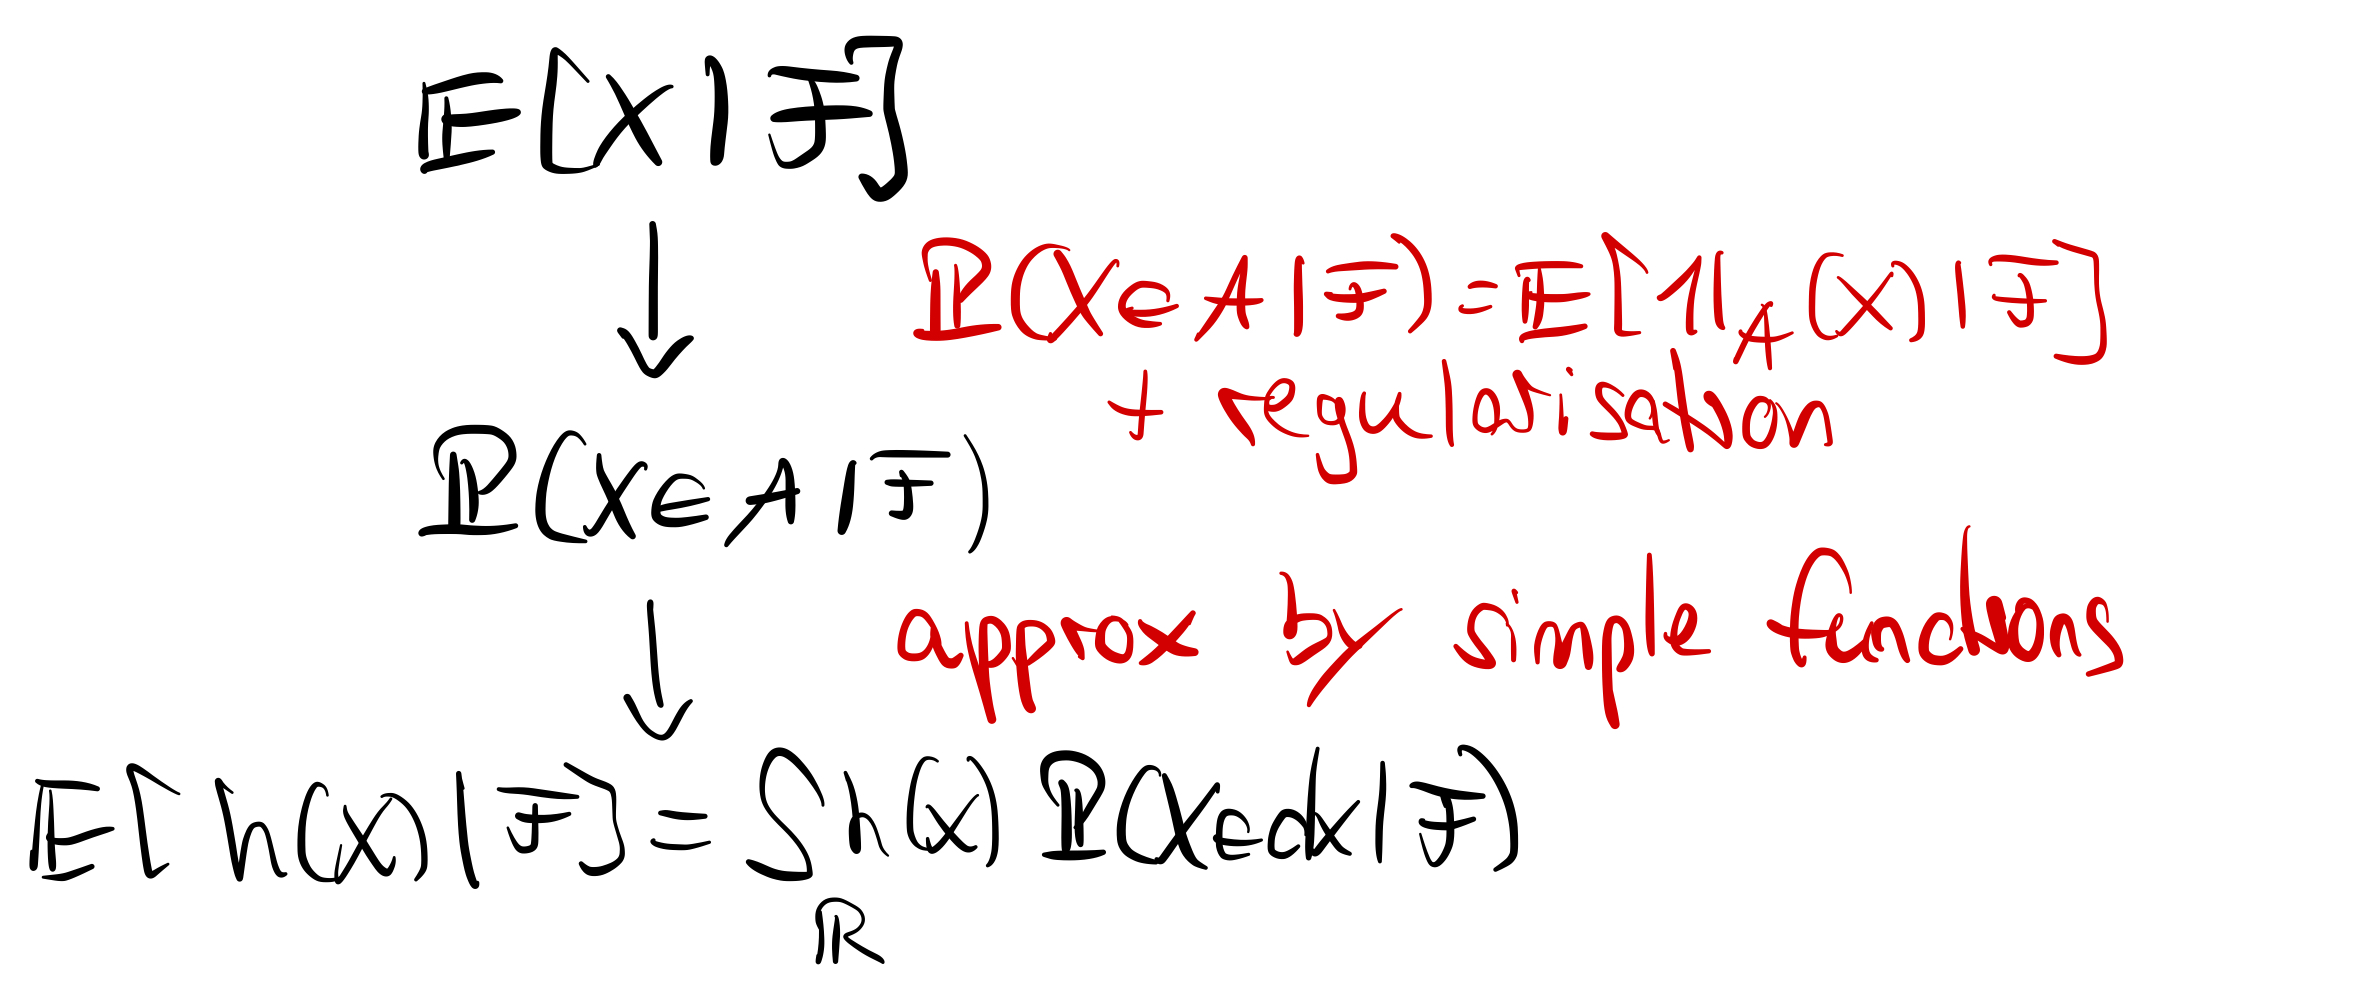
\includegraphics[scale=0.1]{CE10.jpeg}		
%	\end{center}
%		\vspace{-0.3cm}
%	\caption*{The logic behind the regular conditional probability}
%\end{figure}

\begin{figure}[h]
\begin{center}
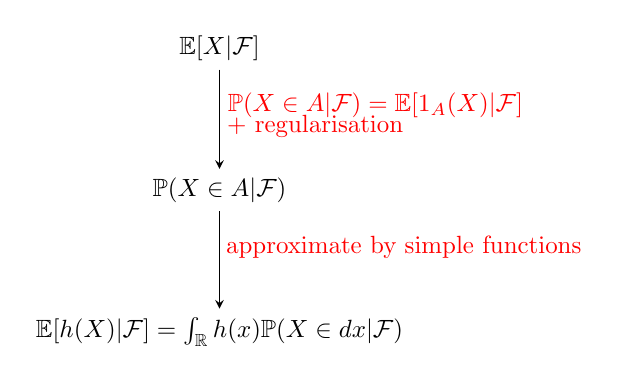
\begin{tikzpicture}[scale=.9,transform shape]
  \node[black,scale=1] (equation1) at (0,0) {$\mathbb{E}[X|\mathcal{F}]$};
  \node[black,scale=1] (equation2) at (0,-2) {$\mathbb{P}(X \in A |\mathcal{F})$};
  \node[black,scale=1] (equation3) at (0,-4) {$\mathbb{E}[h(X)|\mathcal{F}] = \int_{\mathbb{R}} h(x) \mathbb{P}(X \in dx |\mathcal{F})$};
  
  \node[red,scale=1] (txt1) at (2.2,-0.8) {$\mathbb{P}(X \in A |\mathcal{F}) = \mathbb{E}[\mathbbm{1}_A(X) |\mathcal{F}]$};
  \node[red,scale=1] (txt2) at ($(txt1.south) + (-0.85,0)$) {+ regularisation};
  \draw[-stealth,black] (equation1) -- (equation2);
  \node[red,scale=1] (txt2) at (2.6,-2.8) {approximate by simple functions};
  \draw[-stealth,black] (equation2) -- (equation3);
\end{tikzpicture}
  \caption*{The logic behind the regular conditional probability}
\end{center}
\end{figure}


%In virtue of computations performed for classical expectations we can go one step further and also as for conditional densities that allow to compute the random measure $\P_{X|\mathcal F}$ through integrals over random densities.
%\begin{deff}
%	A mapping $f_{X|\mathcal F}:\Omega\times \R\to \R$ is called conditional density of $X$ given $\mathcal F$ if 
%	\begin{itemize}
%		\item $x\mapsto f_{X|\mathcal F}(\omega, x)$ is Borel-measurable for all $\omega\in \Omega$,
%		\item $\omega\mapsto f_{X|\mathcal F}(\omega,x)$ is $\mathcal A$-measurable for all $x\in \R$,
%		\item $\P_{X|\mathcal F}(B)(\omega)=\int_B f_{X|\mathcal F}(\omega,x)\dint x$ a.s. for all $B\in \mathcal B(\R)$.
%	\end{itemize}
%\end{deff}
%Such measurability conditions are certainly frightening on first view. Just keep in mind that all integrals that we possible consider need measurability for the definition. Hence, whenever we see mappings in probability theory we will need measurability. As an example let us come back to the case of jointly absolutely continuous random variables from Proposition \ref{pjc}:
\begin{lwarnhinweis}
As soon as you attend a lecture on general Markov processes, the object of regular conditional expectation will be central to define the Markov property as
\begin{align*}
	\P(X_{t+s}\in A| \mathcal F_t)=\P(X_{t+s}\in A|X_t)\quad\text{a.s.},
\end{align*}
where $\mathcal F_t=\sigma(X_s:s\leq t)$ is the information of the process up to time $t$. This is a way of formalising the idea of the future distribution given the past is equal to the future distribution given the entire past.
\end{lwarnhinweis}

It is typically a good exercise to check Markov inequalities as the proofs require the standard tools of probability theory. Do it!
\begin{luebung}
Let $h:[0,\infty)\to [0,\infty)$ increasing, then
\begin{align*}
	\P(|X|>\epsilon|\mathcal F)\leq \frac{\E[h(X)|\mathcal F]}{h(\epsilon)}\quad \text{a.s.}
\end{align*}
\end{luebung}



%\begin{proof}
%	Define $\nu(y,B) = \int_{B} f_{X|Y}(x,y)\dint x$ and show the defining property for $\nu(Y,B)$: Let $g$ be $\sigma(Y)$-measurable:
%	\begin{align*}
%		\mathds E\big[g(Y)\nu(Y,B)\big]&= \int_{\Omega} g \big( Y(\omega)\big)\nu\big(Y(\omega),B\big)\dint\mathbb{P}(\omega) \\
%								&= \int_{\Omega} g\big(Y(\omega)\big) \int_{B} f_{X|Y}\big(x,Y(\omega)\big)\dint x \dint \mathbb{P}(\omega) \\
%								\overset{\text{no problem, why?}}&{=} \int_{\Omega} \frac{g\big(Y(\omega)\big)}{f_y\big(Y(\omega)\big)} \int_{B}f\big(x,Y(\omega)\big)\dint x \dint \mathbb{P}(\omega)\\
%								&= \int_{\mathbb{R}}\frac{g(Y)}{f_y(y)} \int_{B} f(x,y)\dint x f_y(y)\dint y  \\
%								&= \int_{\mathbb{R}} \int_{\mathbb{R}} g(y)\mathds 1_B(x)f(x,y)\dint x \dint y \\
%								&= \mathds E\big[g(Y)\mathds 1_B(X)\big]
%	\end{align*}
%\end{proof}


	\chapter{Martingale theory}\label{chapter:MT}
	\marginpar{\textcolor{red}{Lecture 4}}


Most probabilists will agree to say their favorite  application of conditional expectation is martingales. In this chapter we will discuss martingale theory in discrete time and, as a rather simple application, give a proof of the strong law of large numbers from Section \ref{sec:GGZ}.

\section[Stochastic processes in discrete time]{Introduction to stochastic processes in discrete time}\label{sec:SP}
Before turning to the special class of martingales we will fix some notation of stochastic processes and prove some elementary facts.

\begin{ldef}
\begin{deff}\label{Def_sto_process}
	Suppose $(\Omega,\cF,\mathbb{P})$ is a probability space, $( E,\mathcal E )$ is a measurable space, and $I$ is an index set. Then a  family of random variables $X=(X_t)_{t \in I}$ on $( \Omega,\cF,\mathbb{P} )$ with values in $(E,\mathcal E )$ is called a \textbf{stochastic process} with values in $E$, called the state-space.
\end{deff}	
\end{ldef}
This is for the first time that we use the name random variable more freely. In Chapter \ref{sec:Stochastik} a random variable was defined to be a real-valued (or $\bar \R$-valued) measurable mapping, a vector-valued random variable was called random vector. From now on we will call  $E$-valued $(\mathcal F, \mathcal E)$-measurable mappings random variables in order to avoid the use of even more notation. Only for $E=\R^d$ we will typically speak of random vectors. Some authors prefer to use the wording random element if the state-space is different from $\R$.\smallskip

	Depending on the index set $I$, stochastic processes are assigned different names. 
	\begin{itemize}
		\item If $|I|=1$, for instance $I=\{1\}$, then a stochastic process indexed by $I$ is nothing but an $E$-valued random variable.
		\item If $|I|=d$, for instance $I=\{1,...,d\}$, then a stochastic process indexed by $I$ is already known under the name random vector. 
		\item A stochastic process indexed by $I=\N,I=\Z$, or $I=\Z^d$ is called a stochastic process in discrete time. 
		\item A stochastic process indexed by $I=\R, I=[0,\infty)$, or $I=[0,T]$ is called stochastic processes in continuous time. 
		\item A stochastic process indexed by $I=\R^d,I=\N^d$, or $I=\Z^d$ is called a random field. 
	\end{itemize}
In most examples of this course we will see values in $E=\R$ or $E=\R^d$ and an index set referring to time (discrete in this section, continuous once we talk about the Brownian motion). In such cases a stochastic process $(X_t)$ might be a model of the (random) time evolution of the price of a stock. However, other interpretations of the states $X_t$ and the index set $I$ are possible. For example, the random variable $X_t:\Omega\to\R^2$ can describe the temperature and air pressure in space, where $t=(u,v,w)\in\R^3$ are the coordinates.
%
%Most of the time we see the ordered index sets 
%\begin{align*}
%	I=\R, \quad I=[0,\infty), \quad I=[0,T]
%\end{align*}
%or
%\begin{align*}
%	I=\Z,\quad  I=\mathbb{N}_0=\lbrace 0,1,2,...\rbrace, \quad I=-\N_0=\{...,-1,0\}, \quad I=\N, \quad I=\{1,...,N\}
%\end{align*}	 
%	  which are interpreted as time. Most of the time there is a first element such as $0$ and we interpret the time running forwards. If there is a last element such as $0$, we speak of a backwards process which is running from the past to present time.
%\begin{ldef}
%\begin{deff}
%	If $I$ is a discrete set (there is no accumulation point), a stochastic process indexed by $I$ is called a \textbf{discrete-time stochastic process}.
%\end{deff}
%\end{ldef}
\begin{ldef}
\begin{deff}
	If $X$ is an $E$-valued stochastic process indexed by $I$, then a realization of all times for fixed $\omega$ $$t\mapsto X_t(\omega)$$ is called a (random) path (or \textbf{sample path}, or \textbf{trajectory}) of $X$. The set of all paths (functions from $I$ to $E$) is denoted by $E^I:=\{f:I\to E\}.$
%	We always equip $E^I$ with the \textbf{$\sigma$-algebra of so-called cylinder sets} generated by the finite projections. That is,
%	\begin{align*}
%		\mathcal E^I:= \sigma( \{\pi_\alpha^{-1}(B):\alpha \subseteq I, |\alpha|<\infty, B\in  \mathcal E^{|\alpha|}\}),
%	\end{align*}
%	where $\pi_\alpha(f)=(f(\alpha_1),...,f(\alpha_{|\alpha|}))$ takes a path and gives the values of the path at finitely many given time points. 
\end{deff}
\end{ldef}
%To get a feeling of the cylinder sets let us fix a vector $\alpha=(\alpha_1,..., \alpha_4)$ of four time points, a Borel-set in $\R^4$ (let's say a four dimensional cube $I_1\times ... \times I_4$) and visualise the corresponding cylinder set: \footnote{bild fehlt}
The notion "{}path"{} of a process mostly makes sense if $I$ is an index set referring to time. If $I$ is interpreted as space it is more reasonable to speak of the realization of a random field instead. In this section we will not go further into the interpretation of stochastic processes as path-valued random variables but instead work with the basic definition of a stochastic process as a family of random variables. In Section \ref{sec:SP} we will go much deeper into alternative interpretations which require quite a bit of additional measure theory.\smallskip

%		It is important for the understanding to keep in mind that $\R^I$ is nothing but $\R^d$ if $|\alpha|=d$. There is no difference between a vector and a mapping with finitely many variables! We also like to use the notation $\R^\infty$ instead of $\R^\N$ and keep in mind that this is just a different notation for the set of real sequences. 
%\begin{lwarnhinweis}
%		The path space $(E^I,\mathcal E^I)$ is a nice measurable space if $I$ is discrete but not nice at all at all if $I$ is not discrete. We will get back to the continuous case only when we start to discuss the Brownian motion. 
%\end{lwarnhinweis}
%	In the discrete-time case one can check just as in Proposition \ref{zweiInterpr} that the notion of a stochastic process as a family of random variables is equivalent to that as a function-valued random variable:
%	\begin{align*}
%		X \text{ is }(\mathcal F,\mathcal E^I)\text{-measurable}\quad \Leftrightarrow\quad X_t \text{ is } (\mathcal F,\mathcal E)\text{-measurable for all }t\in I.
%	\end{align*}	
%	One can prove this fact by checking the measurability on a generator of $\mathcal E^I$, namely the $1$-cylinder sets. To see that the $1$-cylinder sets generate $%\mathcal E^I$ one only needs to note that all cylinder sets can be obtained by intersecting $1$-cylinder sets.\smallskip

Here are some examples of stochastic processes:
\begin{example}
	\begin{enumerate}[label=(\roman*)]
		\item Every sequence of random variables (e.g. iid) $X_1, X_2,...$ defines a stochastic process indexed by $\N$.
\begin{figure}[h]
\begin{center}
		\scalebox{0.8}{
  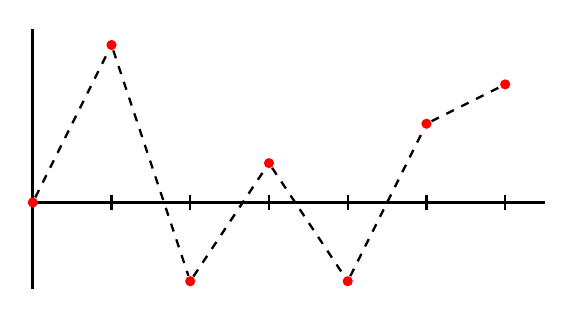
\begin{tikzpicture}
  \tikzset{
    pics/tick/.style args={#1}{code={
      \draw[line width=0.3mm] (0,-#1) -- (0,#1) ;
      },
    }
  }
  
    %AXIS Y
    \draw[line width=0.4mm] (0,-1.1) -- ++(90:3.3cm);
    %AXIS X 
    \draw[line width=0.4mm] (0,0) --++(0:6.5cm);
  
    \draw (0,0) pic {tick={1mm}} node[circle,inner sep=1.3pt,fill=red,yshift=0cm] (0) {};
    \draw (1,0) pic {tick={1mm}} node[circle,inner sep=1.3pt,fill=red,yshift=2cm] (1) {};
    \draw (2,0) pic {tick={1mm}} node[circle,inner sep=1.3pt,fill=red,yshift=-1cm] (2) {};
    \draw (3,0) pic {tick={1mm}} node[circle,inner sep=1.3pt,fill=red,yshift=0.5cm] (3) {};
    \draw (4,0) pic {tick={1mm}} node[circle,inner sep=1.3pt,fill=red,yshift=-1cm]  (4) {};
    \draw (5,0) pic {tick={1mm}} node[circle,inner sep=1.3pt,fill=red,yshift=1cm] (5) {};
    \draw (6,0) pic {tick={1mm}} node[circle,inner sep=1.3pt,fill=red,yshift=1.5cm] (6) {};
    \foreach \x/\y in {0/1,1/2,2/3,3/4,4/5,5/6} {
      \draw[dashed,line width=0.3mm] (\x) -- (\y) ;
    }
  \end{tikzpicture} 
  }
\end{center}
\end{figure}
Since there is no dependence between the values at different times the paths can look completely wild.  
		\item Here is a path of the so-called Brownian motion, indexed by $I=[0,\infty)$ that we will get to know later in this course.
			\begin{figure}[H]
				% Created by tikzDevice version 0.12.3.1 on 2021-08-23 21:22:56
% !TEX encoding = UTF-8 Unicode
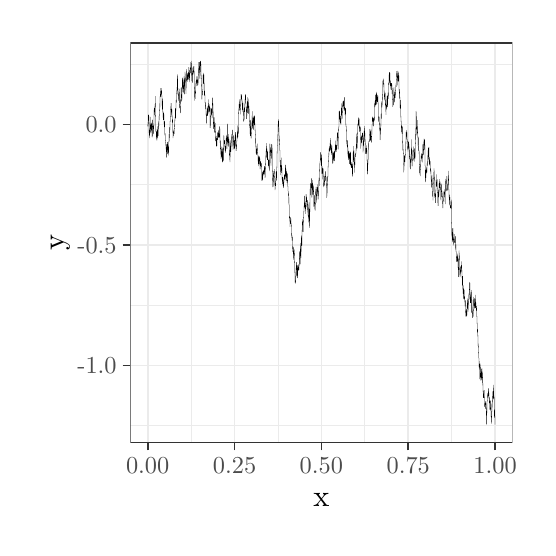
\begin{tikzpicture}[x=1pt,y=1pt]
\definecolor{fillColor}{RGB}{255,255,255}
\path[use as bounding box,fill=fillColor,fill opacity=0.00] (0,0) rectangle (180.67,180.67);
\begin{scope}
\path[clip] (  0.00,  0.00) rectangle (180.67,180.67);
\definecolor{drawColor}{RGB}{255,255,255}
\definecolor{fillColor}{RGB}{255,255,255}

\path[draw=drawColor,line width= 0.6pt,line join=round,line cap=round,fill=fillColor] (  0.00,  0.00) rectangle (180.67,180.68);
\end{scope}
\begin{scope}
\path[clip] ( 37.09, 30.69) rectangle (175.17,175.17);
\definecolor{fillColor}{RGB}{255,255,255}

\path[fill=fillColor] ( 37.09, 30.69) rectangle (175.17,175.17);
\definecolor{drawColor}{gray}{0.92}

\path[draw=drawColor,line width= 0.3pt,line join=round] ( 37.09, 36.88) --
	(175.17, 36.88);

\path[draw=drawColor,line width= 0.3pt,line join=round] ( 37.09, 80.41) --
	(175.17, 80.41);

\path[draw=drawColor,line width= 0.3pt,line join=round] ( 37.09,123.94) --
	(175.17,123.94);

\path[draw=drawColor,line width= 0.3pt,line join=round] ( 37.09,167.47) --
	(175.17,167.47);

\path[draw=drawColor,line width= 0.3pt,line join=round] ( 59.06, 30.69) --
	( 59.06,175.17);

\path[draw=drawColor,line width= 0.3pt,line join=round] ( 90.44, 30.69) --
	( 90.44,175.17);

\path[draw=drawColor,line width= 0.3pt,line join=round] (121.82, 30.69) --
	(121.82,175.17);

\path[draw=drawColor,line width= 0.3pt,line join=round] (153.21, 30.69) --
	(153.21,175.17);

\path[draw=drawColor,line width= 0.6pt,line join=round] ( 37.09, 58.64) --
	(175.17, 58.64);

\path[draw=drawColor,line width= 0.6pt,line join=round] ( 37.09,102.17) --
	(175.17,102.17);

\path[draw=drawColor,line width= 0.6pt,line join=round] ( 37.09,145.70) --
	(175.17,145.70);

\path[draw=drawColor,line width= 0.6pt,line join=round] ( 43.37, 30.69) --
	( 43.37,175.17);

\path[draw=drawColor,line width= 0.6pt,line join=round] ( 74.75, 30.69) --
	( 74.75,175.17);

\path[draw=drawColor,line width= 0.6pt,line join=round] (106.13, 30.69) --
	(106.13,175.17);

\path[draw=drawColor,line width= 0.6pt,line join=round] (137.52, 30.69) --
	(137.52,175.17);

\path[draw=drawColor,line width= 0.6pt,line join=round] (168.90, 30.69) --
	(168.90,175.17);
\definecolor{drawColor}{RGB}{0,0,0}

\path[draw=drawColor,line width= 0.1pt,line join=round] ( 43.37,145.70) --
	( 43.40,145.16) --
	( 43.44,145.04) --
	( 43.47,145.60) --
	( 43.51,145.11) --
	( 43.54,147.39) --
	( 43.58,148.60) --
	( 43.62,149.20) --
	( 43.65,147.75) --
	( 43.69,147.15) --
	( 43.72,148.89) --
	( 43.76,149.06) --
	( 43.80,148.52) --
	( 43.83,145.23) --
	( 43.87,144.63) --
	( 43.90,141.74) --
	( 43.94,141.50) --
	( 43.98,141.69) --
	( 44.01,140.82) --
	( 44.05,142.57) --
	( 44.08,143.58) --
	( 44.12,141.87) --
	( 44.15,144.09) --
	( 44.19,144.38) --
	( 44.23,146.44) --
	( 44.26,145.81) --
	( 44.30,148.37) --
	( 44.33,146.10) --
	( 44.37,144.81) --
	( 44.41,144.22) --
	( 44.44,142.54) --
	( 44.48,144.04) --
	( 44.51,144.24) --
	( 44.55,143.77) --
	( 44.58,142.83) --
	( 44.62,146.18) --
	( 44.66,143.44) --
	( 44.69,143.63) --
	( 44.73,145.02) --
	( 44.76,146.27) --
	( 44.80,145.49) --
	( 44.84,145.59) --
	( 44.87,145.13) --
	( 44.91,144.41) --
	( 44.94,141.11) --
	( 44.98,141.39) --
	( 45.02,141.94) --
	( 45.05,141.19) --
	( 45.09,143.94) --
	( 45.12,147.29) --
	( 45.16,147.36) --
	( 45.19,146.74) --
	( 45.23,145.71) --
	( 45.27,146.05) --
	( 45.30,146.02) --
	( 45.34,144.61) --
	( 45.37,142.52) --
	( 45.41,143.41) --
	( 45.45,142.23) --
	( 45.48,143.06) --
	( 45.52,144.60) --
	( 45.55,144.16) --
	( 45.59,144.78) --
	( 45.62,146.01) --
	( 45.66,148.26) --
	( 45.70,151.32) --
	( 45.73,151.00) --
	( 45.77,151.54) --
	( 45.80,149.10) --
	( 45.84,150.08) --
	( 45.88,150.24) --
	( 45.91,151.70) --
	( 45.95,151.77) --
	( 45.98,152.35) --
	( 46.02,152.66) --
	( 46.06,153.19) --
	( 46.09,155.87) --
	( 46.13,153.89) --
	( 46.16,152.28) --
	( 46.20,151.00) --
	( 46.23,149.05) --
	( 46.27,146.68) --
	( 46.31,143.29) --
	( 46.34,143.16) --
	( 46.38,144.01) --
	( 46.41,143.10) --
	( 46.45,142.63) --
	( 46.49,142.03) --
	( 46.52,140.67) --
	( 46.56,141.06) --
	( 46.59,140.92) --
	( 46.63,143.19) --
	( 46.67,140.36) --
	( 46.70,139.93) --
	( 46.74,140.98) --
	( 46.77,141.38) --
	( 46.81,142.83) --
	( 46.84,144.99) --
	( 46.88,143.02) --
	( 46.92,141.74) --
	( 46.95,142.54) --
	( 46.99,143.69) --
	( 47.02,140.81) --
	( 47.06,141.97) --
	( 47.10,142.44) --
	( 47.13,141.56) --
	( 47.17,141.97) --
	( 47.20,142.74) --
	( 47.24,145.63) --
	( 47.27,144.03) --
	( 47.31,146.13) --
	( 47.35,146.84) --
	( 47.38,146.18) --
	( 47.42,145.17) --
	( 47.45,147.43) --
	( 47.49,148.82) --
	( 47.53,147.36) --
	( 47.56,148.42) --
	( 47.60,149.35) --
	( 47.63,150.01) --
	( 47.67,150.36) --
	( 47.71,152.31) --
	( 47.74,153.29) --
	( 47.78,152.63) --
	( 47.81,151.90) --
	( 47.85,155.65) --
	( 47.88,155.97) --
	( 47.92,155.58) --
	( 47.96,156.84) --
	( 47.99,158.76) --
	( 48.03,155.68) --
	( 48.06,156.32) --
	( 48.10,156.21) --
	( 48.14,157.13) --
	( 48.17,157.36) --
	( 48.21,157.47) --
	( 48.24,157.99) --
	( 48.28,158.81) --
	( 48.31,157.19) --
	( 48.35,156.43) --
	( 48.39,156.90) --
	( 48.42,157.90) --
	( 48.46,157.22) --
	( 48.49,156.16) --
	( 48.53,153.77) --
	( 48.57,152.79) --
	( 48.60,152.35) --
	( 48.64,151.18) --
	( 48.67,153.97) --
	( 48.71,153.72) --
	( 48.75,155.01) --
	( 48.78,152.24) --
	( 48.82,150.78) --
	( 48.85,150.58) --
	( 48.89,148.22) --
	( 48.92,148.94) --
	( 48.96,147.93) --
	( 49.00,149.09) --
	( 49.03,147.37) --
	( 49.07,149.92) --
	( 49.10,149.22) --
	( 49.14,149.90) --
	( 49.18,148.91) --
	( 49.21,147.63) --
	( 49.25,149.27) --
	( 49.28,146.33) --
	( 49.32,145.70) --
	( 49.36,144.93) --
	( 49.39,144.81) --
	( 49.43,146.41) --
	( 49.46,146.83) --
	( 49.50,146.66) --
	( 49.53,144.15) --
	( 49.57,142.14) --
	( 49.61,141.73) --
	( 49.64,141.88) --
	( 49.68,142.42) --
	( 49.71,141.39) --
	( 49.75,139.95) --
	( 49.79,139.30) --
	( 49.82,139.23) --
	( 49.86,139.00) --
	( 49.89,138.21) --
	( 49.93,138.97) --
	( 49.96,136.77) --
	( 50.00,137.54) --
	( 50.04,137.56) --
	( 50.07,135.97) --
	( 50.11,133.78) --
	( 50.14,134.12) --
	( 50.18,136.12) --
	( 50.22,135.83) --
	( 50.25,137.58) --
	( 50.29,138.38) --
	( 50.32,138.51) --
	( 50.36,138.54) --
	( 50.40,136.04) --
	( 50.43,135.59) --
	( 50.47,135.03) --
	( 50.50,135.84) --
	( 50.54,138.52) --
	( 50.57,139.34) --
	( 50.61,137.75) --
	( 50.65,136.47) --
	( 50.68,137.55) --
	( 50.72,137.02) --
	( 50.75,136.62) --
	( 50.79,136.74) --
	( 50.83,134.52) --
	( 50.86,137.98) --
	( 50.90,137.53) --
	( 50.93,135.65) --
	( 50.97,137.57) --
	( 51.00,138.93) --
	( 51.04,139.88) --
	( 51.08,142.13) --
	( 51.11,140.01) --
	( 51.15,140.18) --
	( 51.18,139.76) --
	( 51.22,142.25) --
	( 51.26,144.64) --
	( 51.29,144.64) --
	( 51.33,142.74) --
	( 51.36,142.56) --
	( 51.40,144.88) --
	( 51.44,145.36) --
	( 51.47,146.72) --
	( 51.51,147.66) --
	( 51.54,148.08) --
	( 51.58,148.94) --
	( 51.61,149.97) --
	( 51.65,151.20) --
	( 51.69,151.25) --
	( 51.72,151.08) --
	( 51.76,152.59) --
	( 51.79,151.76) --
	( 51.83,153.38) --
	( 51.87,153.25) --
	( 51.90,151.46) --
	( 51.94,149.65) --
	( 51.97,150.08) --
	( 52.01,149.49) --
	( 52.05,148.55) --
	( 52.08,151.29) --
	( 52.12,150.93) --
	( 52.15,149.17) --
	( 52.19,148.95) --
	( 52.22,147.32) --
	( 52.26,146.44) --
	( 52.30,147.17) --
	( 52.33,147.35) --
	( 52.37,147.50) --
	( 52.40,144.98) --
	( 52.44,144.33) --
	( 52.48,142.33) --
	( 52.51,140.81) --
	( 52.55,142.41) --
	( 52.58,143.81) --
	( 52.62,143.07) --
	( 52.65,142.48) --
	( 52.69,143.22) --
	( 52.73,143.19) --
	( 52.76,141.57) --
	( 52.80,141.68) --
	( 52.83,142.32) --
	( 52.87,142.78) --
	( 52.91,142.35) --
	( 52.94,142.28) --
	( 52.98,143.96) --
	( 53.01,144.35) --
	( 53.05,144.19) --
	( 53.09,145.64) --
	( 53.12,145.02) --
	( 53.16,144.83) --
	( 53.19,147.31) --
	( 53.23,148.36) --
	( 53.26,147.77) --
	( 53.30,148.25) --
	( 53.34,148.49) --
	( 53.37,151.48) --
	( 53.41,148.81) --
	( 53.44,149.17) --
	( 53.48,148.69) --
	( 53.52,147.96) --
	( 53.55,151.00) --
	( 53.59,153.01) --
	( 53.62,154.43) --
	( 53.66,154.54) --
	( 53.69,153.86) --
	( 53.73,153.67) --
	( 53.77,154.33) --
	( 53.80,156.72) --
	( 53.84,156.92) --
	( 53.87,156.81) --
	( 53.91,157.73) --
	( 53.95,159.09) --
	( 53.98,156.79) --
	( 54.02,158.82) --
	( 54.05,163.18) --
	( 54.09,161.36) --
	( 54.13,163.71) --
	( 54.16,163.32) --
	( 54.20,160.91) --
	( 54.23,161.03) --
	( 54.27,158.75) --
	( 54.30,156.43) --
	( 54.34,157.78) --
	( 54.38,157.57) --
	( 54.41,157.16) --
	( 54.45,156.18) --
	( 54.48,156.88) --
	( 54.52,156.44) --
	( 54.56,154.23) --
	( 54.59,155.39) --
	( 54.63,156.03) --
	( 54.66,156.10) --
	( 54.70,156.41) --
	( 54.74,153.42) --
	( 54.77,156.72) --
	( 54.81,156.76) --
	( 54.84,158.55) --
	( 54.88,154.45) --
	( 54.91,151.75) --
	( 54.95,152.95) --
	( 54.99,152.34) --
	( 55.02,151.57) --
	( 55.06,151.46) --
	( 55.09,152.19) --
	( 55.13,151.05) --
	( 55.17,149.82) --
	( 55.20,151.65) --
	( 55.24,154.66) --
	( 55.27,153.29) --
	( 55.31,154.73) --
	( 55.34,153.24) --
	( 55.38,155.19) --
	( 55.42,156.88) --
	( 55.45,159.04) --
	( 55.49,155.31) --
	( 55.52,155.32) --
	( 55.56,156.03) --
	( 55.60,156.54) --
	( 55.63,155.52) --
	( 55.67,154.14) --
	( 55.70,155.22) --
	( 55.74,154.66) --
	( 55.78,157.74) --
	( 55.81,158.85) --
	( 55.85,161.24) --
	( 55.88,162.59) --
	( 55.92,162.23) --
	( 55.95,161.53) --
	( 55.99,161.52) --
	( 56.03,161.83) --
	( 56.06,160.76) --
	( 56.10,158.22) --
	( 56.13,157.54) --
	( 56.17,159.74) --
	( 56.21,158.58) --
	( 56.24,159.30) --
	( 56.28,159.49) --
	( 56.31,161.02) --
	( 56.35,159.20) --
	( 56.38,157.08) --
	( 56.42,160.67) --
	( 56.46,162.45) --
	( 56.49,163.00) --
	( 56.53,162.44) --
	( 56.56,160.31) --
	( 56.60,159.78) --
	( 56.64,159.34) --
	( 56.67,158.27) --
	( 56.71,156.64) --
	( 56.74,158.47) --
	( 56.78,161.15) --
	( 56.82,162.20) --
	( 56.85,164.65) --
	( 56.89,164.03) --
	( 56.92,163.25) --
	( 56.96,163.17) --
	( 56.99,162.32) --
	( 57.03,161.10) --
	( 57.07,160.88) --
	( 57.10,161.49) --
	( 57.14,160.08) --
	( 57.17,157.97) --
	( 57.21,156.81) --
	( 57.25,158.78) --
	( 57.28,159.39) --
	( 57.32,160.25) --
	( 57.35,161.88) --
	( 57.39,165.04) --
	( 57.43,164.79) --
	( 57.46,165.63) --
	( 57.50,164.16) --
	( 57.53,162.53) --
	( 57.57,161.91) --
	( 57.60,162.26) --
	( 57.64,161.17) --
	( 57.68,162.04) --
	( 57.71,164.12) --
	( 57.75,162.70) --
	( 57.78,163.15) --
	( 57.82,163.57) --
	( 57.86,162.41) --
	( 57.89,161.91) --
	( 57.93,162.51) --
	( 57.96,162.81) --
	( 58.00,163.13) --
	( 58.03,164.49) --
	( 58.07,162.32) --
	( 58.11,162.04) --
	( 58.14,162.22) --
	( 58.18,164.48) --
	( 58.21,166.37) --
	( 58.25,165.11) --
	( 58.29,164.75) --
	( 58.32,164.04) --
	( 58.36,165.19) --
	( 58.39,164.83) --
	( 58.43,162.54) --
	( 58.47,163.31) --
	( 58.50,162.73) --
	( 58.54,161.04) --
	( 58.57,163.86) --
	( 58.61,164.22) --
	( 58.64,164.27) --
	( 58.68,166.08) --
	( 58.72,166.35) --
	( 58.75,165.62) --
	( 58.79,165.63) --
	( 58.82,168.20) --
	( 58.86,166.67) --
	( 58.90,165.20) --
	( 58.93,165.04) --
	( 58.97,164.28) --
	( 59.00,165.26) --
	( 59.04,164.93) --
	( 59.07,165.76) --
	( 59.11,168.59) --
	( 59.15,167.79) --
	( 59.18,165.80) --
	( 59.22,163.63) --
	( 59.25,163.46) --
	( 59.29,161.52) --
	( 59.33,161.39) --
	( 59.36,161.70) --
	( 59.40,163.37) --
	( 59.43,164.22) --
	( 59.47,163.97) --
	( 59.51,160.84) --
	( 59.54,163.32) --
	( 59.58,164.47) --
	( 59.61,165.03) --
	( 59.65,166.14) --
	( 59.68,163.74) --
	( 59.72,164.52) --
	( 59.76,165.15) --
	( 59.79,165.07) --
	( 59.83,164.62) --
	( 59.86,163.81) --
	( 59.90,165.71) --
	( 59.94,166.35) --
	( 59.97,166.61) --
	( 60.01,165.87) --
	( 60.04,165.01) --
	( 60.08,166.78) --
	( 60.12,165.46) --
	( 60.15,164.81) --
	( 60.19,160.77) --
	( 60.22,160.39) --
	( 60.26,156.62) --
	( 60.29,154.38) --
	( 60.33,155.75) --
	( 60.37,157.16) --
	( 60.40,156.78) --
	( 60.44,157.71) --
	( 60.47,157.91) --
	( 60.51,157.20) --
	( 60.55,157.06) --
	( 60.58,157.36) --
	( 60.62,157.41) --
	( 60.65,154.99) --
	( 60.69,157.20) --
	( 60.72,159.53) --
	( 60.76,160.12) --
	( 60.80,160.77) --
	( 60.83,161.22) --
	( 60.87,161.35) --
	( 60.90,161.67) --
	( 60.94,160.87) --
	( 60.98,160.88) --
	( 61.01,163.05) --
	( 61.05,161.77) --
	( 61.08,160.03) --
	( 61.12,159.58) --
	( 61.16,160.19) --
	( 61.19,161.14) --
	( 61.23,161.65) --
	( 61.26,160.88) --
	( 61.30,161.40) --
	( 61.33,161.29) --
	( 61.37,161.30) --
	( 61.41,161.84) --
	( 61.44,163.02) --
	( 61.48,159.76) --
	( 61.51,160.60) --
	( 61.55,160.02) --
	( 61.59,160.69) --
	( 61.62,160.88) --
	( 61.66,162.69) --
	( 61.69,163.94) --
	( 61.73,165.92) --
	( 61.76,165.10) --
	( 61.80,165.77) --
	( 61.84,168.15) --
	( 61.87,164.22) --
	( 61.91,165.01) --
	( 61.94,164.77) --
	( 61.98,167.92) --
	( 62.02,167.96) --
	( 62.05,168.19) --
	( 62.09,166.27) --
	( 62.12,166.85) --
	( 62.16,166.23) --
	( 62.20,164.06) --
	( 62.23,162.22) --
	( 62.27,162.96) --
	( 62.30,164.62) --
	( 62.34,165.12) --
	( 62.37,165.36) --
	( 62.41,168.57) --
	( 62.45,167.35) --
	( 62.48,168.61) --
	( 62.52,168.11) --
	( 62.55,166.92) --
	( 62.59,167.60) --
	( 62.63,164.76) --
	( 62.66,163.77) --
	( 62.70,163.01) --
	( 62.73,162.74) --
	( 62.77,162.30) --
	( 62.81,162.21) --
	( 62.84,161.01) --
	( 62.88,157.95) --
	( 62.91,157.94) --
	( 62.95,154.80) --
	( 62.98,157.73) --
	( 63.02,156.96) --
	( 63.06,156.43) --
	( 63.09,157.47) --
	( 63.13,156.34) --
	( 63.16,156.61) --
	( 63.20,157.60) --
	( 63.24,157.87) --
	( 63.27,157.72) --
	( 63.31,158.18) --
	( 63.34,161.95) --
	( 63.38,163.52) --
	( 63.41,161.92) --
	( 63.45,162.39) --
	( 63.49,161.44) --
	( 63.52,160.53) --
	( 63.56,162.60) --
	( 63.59,164.27) --
	( 63.63,164.22) --
	( 63.67,163.65) --
	( 63.70,161.38) --
	( 63.74,160.36) --
	( 63.77,160.70) --
	( 63.81,158.73) --
	( 63.85,156.17) --
	( 63.88,157.17) --
	( 63.92,157.87) --
	( 63.95,157.59) --
	( 63.99,157.13) --
	( 64.02,156.50) --
	( 64.06,156.04) --
	( 64.10,154.08) --
	( 64.13,153.37) --
	( 64.17,153.64) --
	( 64.20,152.86) --
	( 64.24,151.40) --
	( 64.28,153.62) --
	( 64.31,151.15) --
	( 64.35,152.48) --
	( 64.38,151.97) --
	( 64.42,150.62) --
	( 64.45,149.93) --
	( 64.49,148.95) --
	( 64.53,150.35) --
	( 64.56,149.86) --
	( 64.60,148.77) --
	( 64.63,147.97) --
	( 64.67,146.08) --
	( 64.71,146.81) --
	( 64.74,148.72) --
	( 64.78,149.11) --
	( 64.81,148.87) --
	( 64.85,149.20) --
	( 64.89,149.94) --
	( 64.92,150.68) --
	( 64.96,152.20) --
	( 64.99,149.74) --
	( 65.03,149.70) --
	( 65.06,150.46) --
	( 65.10,148.83) --
	( 65.14,151.63) --
	( 65.17,150.72) --
	( 65.21,151.52) --
	( 65.24,149.83) --
	( 65.28,151.81) --
	( 65.32,153.19) --
	( 65.35,154.74) --
	( 65.39,152.95) --
	( 65.42,153.24) --
	( 65.46,152.51) --
	( 65.50,151.19) --
	( 65.53,151.93) --
	( 65.57,150.24) --
	( 65.60,150.53) --
	( 65.64,151.43) --
	( 65.67,151.90) --
	( 65.71,152.19) --
	( 65.75,150.78) --
	( 65.78,150.88) --
	( 65.82,152.92) --
	( 65.85,150.35) --
	( 65.89,146.89) --
	( 65.93,144.44) --
	( 65.96,144.58) --
	( 66.00,144.93) --
	( 66.03,145.65) --
	( 66.07,148.04) --
	( 66.10,148.38) --
	( 66.14,148.88) --
	( 66.18,148.54) --
	( 66.21,149.14) --
	( 66.25,150.41) --
	( 66.28,151.62) --
	( 66.32,151.45) --
	( 66.36,149.40) --
	( 66.39,149.67) --
	( 66.43,150.36) --
	( 66.46,150.91) --
	( 66.50,149.59) --
	( 66.54,151.29) --
	( 66.57,148.71) --
	( 66.61,147.91) --
	( 66.64,147.95) --
	( 66.68,149.54) --
	( 66.71,151.75) --
	( 66.75,153.58) --
	( 66.79,154.39) --
	( 66.82,155.35) --
	( 66.86,154.92) --
	( 66.89,155.17) --
	( 66.93,152.28) --
	( 66.97,151.56) --
	( 67.00,150.63) --
	( 67.04,148.90) --
	( 67.07,148.14) --
	( 67.11,145.76) --
	( 67.14,144.22) --
	( 67.18,145.17) --
	( 67.22,145.26) --
	( 67.25,144.15) --
	( 67.29,145.17) --
	( 67.32,145.27) --
	( 67.36,148.21) --
	( 67.40,148.22) --
	( 67.43,147.16) --
	( 67.47,146.36) --
	( 67.50,146.51) --
	( 67.54,142.79) --
	( 67.58,143.59) --
	( 67.61,145.17) --
	( 67.65,145.59) --
	( 67.68,145.45) --
	( 67.72,144.22) --
	( 67.75,146.19) --
	( 67.79,145.07) --
	( 67.83,142.69) --
	( 67.86,142.33) --
	( 67.90,139.78) --
	( 67.93,139.97) --
	( 67.97,139.73) --
	( 68.01,140.11) --
	( 68.04,139.64) --
	( 68.08,140.71) --
	( 68.11,141.56) --
	( 68.15,138.59) --
	( 68.19,137.80) --
	( 68.22,138.99) --
	( 68.26,139.81) --
	( 68.29,140.68) --
	( 68.33,140.15) --
	( 68.36,139.63) --
	( 68.40,137.96) --
	( 68.44,140.64) --
	( 68.47,140.51) --
	( 68.51,140.26) --
	( 68.54,140.35) --
	( 68.58,140.65) --
	( 68.62,142.53) --
	( 68.65,142.82) --
	( 68.69,140.21) --
	( 68.72,141.25) --
	( 68.76,142.57) --
	( 68.79,142.58) --
	( 68.83,141.48) --
	( 68.87,142.45) --
	( 68.90,140.98) --
	( 68.94,142.27) --
	( 68.97,143.66) --
	( 69.01,143.06) --
	( 69.05,143.31) --
	( 69.08,141.09) --
	( 69.12,142.04) --
	( 69.15,141.01) --
	( 69.19,142.30) --
	( 69.23,141.60) --
	( 69.26,141.11) --
	( 69.30,141.36) --
	( 69.33,144.15) --
	( 69.37,144.80) --
	( 69.40,145.07) --
	( 69.44,144.47) --
	( 69.48,142.82) --
	( 69.51,142.45) --
	( 69.55,138.67) --
	( 69.58,136.92) --
	( 69.62,139.88) --
	( 69.66,139.33) --
	( 69.69,138.39) --
	( 69.73,136.50) --
	( 69.76,136.18) --
	( 69.80,136.78) --
	( 69.83,133.34) --
	( 69.87,135.62) --
	( 69.91,133.49) --
	( 69.94,133.73) --
	( 69.98,133.75) --
	( 70.01,134.97) --
	( 70.05,136.36) --
	( 70.09,136.77) --
	( 70.12,136.79) --
	( 70.16,137.65) --
	( 70.19,135.76) --
	( 70.23,137.48) --
	( 70.27,133.79) --
	( 70.30,132.07) --
	( 70.34,134.49) --
	( 70.37,135.82) --
	( 70.41,134.23) --
	( 70.44,133.07) --
	( 70.48,132.33) --
	( 70.52,136.93) --
	( 70.55,136.86) --
	( 70.59,135.31) --
	( 70.62,134.21) --
	( 70.66,133.02) --
	( 70.70,132.50) --
	( 70.73,133.26) --
	( 70.77,134.94) --
	( 70.80,136.61) --
	( 70.84,139.34) --
	( 70.88,141.73) --
	( 70.91,141.31) --
	( 70.95,139.61) --
	( 70.98,139.86) --
	( 71.02,139.85) --
	( 71.05,138.70) --
	( 71.09,138.70) --
	( 71.13,139.91) --
	( 71.16,139.96) --
	( 71.20,139.14) --
	( 71.23,137.53) --
	( 71.27,137.92) --
	( 71.31,136.25) --
	( 71.34,136.37) --
	( 71.38,137.29) --
	( 71.41,137.48) --
	( 71.45,137.03) --
	( 71.48,137.78) --
	( 71.52,136.06) --
	( 71.56,135.45) --
	( 71.59,138.29) --
	( 71.63,138.58) --
	( 71.66,140.62) --
	( 71.70,140.10) --
	( 71.74,140.15) --
	( 71.77,140.79) --
	( 71.81,140.34) --
	( 71.84,139.81) --
	( 71.88,141.90) --
	( 71.92,138.46) --
	( 71.95,137.26) --
	( 71.99,136.87) --
	( 72.02,139.56) --
	( 72.06,138.69) --
	( 72.09,139.67) --
	( 72.13,143.93) --
	( 72.17,145.91) --
	( 72.20,143.39) --
	( 72.24,140.98) --
	( 72.27,141.22) --
	( 72.31,139.48) --
	( 72.35,139.43) --
	( 72.38,138.09) --
	( 72.42,140.02) --
	( 72.45,139.60) --
	( 72.49,140.72) --
	( 72.52,141.04) --
	( 72.56,142.13) --
	( 72.60,140.89) --
	( 72.63,137.67) --
	( 72.67,139.17) --
	( 72.70,138.75) --
	( 72.74,140.41) --
	( 72.78,140.05) --
	( 72.81,138.46) --
	( 72.85,134.54) --
	( 72.88,136.46) --
	( 72.92,135.98) --
	( 72.96,135.74) --
	( 72.99,133.88) --
	( 73.03,133.09) --
	( 73.06,132.98) --
	( 73.10,132.14) --
	( 73.13,133.23) --
	( 73.17,134.63) --
	( 73.21,136.27) --
	( 73.24,137.40) --
	( 73.28,139.92) --
	( 73.31,138.16) --
	( 73.35,138.99) --
	( 73.39,137.16) --
	( 73.42,135.83) --
	( 73.46,137.29) --
	( 73.49,136.94) --
	( 73.53,138.37) --
	( 73.57,139.28) --
	( 73.60,139.10) --
	( 73.64,140.76) --
	( 73.67,141.25) --
	( 73.71,140.09) --
	( 73.74,139.92) --
	( 73.78,142.00) --
	( 73.82,142.23) --
	( 73.85,141.89) --
	( 73.89,142.22) --
	( 73.92,143.35) --
	( 73.96,143.75) --
	( 74.00,142.68) --
	( 74.03,142.74) --
	( 74.07,140.23) --
	( 74.10,137.83) --
	( 74.14,137.98) --
	( 74.17,138.46) --
	( 74.21,136.45) --
	( 74.25,137.10) --
	( 74.28,138.19) --
	( 74.32,139.41) --
	( 74.35,140.28) --
	( 74.39,141.73) --
	( 74.43,141.39) --
	( 74.46,141.20) --
	( 74.50,141.60) --
	( 74.53,139.57) --
	( 74.57,138.77) --
	( 74.61,138.08) --
	( 74.64,137.14) --
	( 74.68,138.20) --
	( 74.71,137.20) --
	( 74.75,138.20) --
	( 74.78,139.95) --
	( 74.82,136.83) --
	( 74.86,137.50) --
	( 74.89,138.30) --
	( 74.93,139.22) --
	( 74.96,139.82) --
	( 75.00,140.15) --
	( 75.04,141.12) --
	( 75.07,142.83) --
	( 75.11,142.62) --
	( 75.14,142.83) --
	( 75.18,140.69) --
	( 75.21,138.12) --
	( 75.25,138.03) --
	( 75.29,137.71) --
	( 75.32,136.18) --
	( 75.36,136.91) --
	( 75.39,137.84) --
	( 75.43,136.89) --
	( 75.47,138.15) --
	( 75.50,138.62) --
	( 75.54,137.82) --
	( 75.57,139.09) --
	( 75.61,140.21) --
	( 75.65,141.65) --
	( 75.68,141.10) --
	( 75.72,142.03) --
	( 75.75,141.48) --
	( 75.79,143.34) --
	( 75.82,140.75) --
	( 75.86,141.89) --
	( 75.90,142.41) --
	( 75.93,145.28) --
	( 75.97,143.92) --
	( 76.00,141.15) --
	( 76.04,143.42) --
	( 76.08,143.54) --
	( 76.11,142.30) --
	( 76.15,142.77) --
	( 76.18,145.35) --
	( 76.22,149.51) --
	( 76.26,151.41) --
	( 76.29,150.36) --
	( 76.33,150.86) --
	( 76.36,152.36) --
	( 76.40,152.64) --
	( 76.43,153.92) --
	( 76.47,151.78) --
	( 76.51,153.76) --
	( 76.54,154.68) --
	( 76.58,153.08) --
	( 76.61,152.50) --
	( 76.65,152.65) --
	( 76.69,150.58) --
	( 76.72,150.80) --
	( 76.76,151.41) --
	( 76.79,149.38) --
	( 76.83,150.31) --
	( 76.86,151.28) --
	( 76.90,152.88) --
	( 76.94,152.04) --
	( 76.97,153.42) --
	( 77.01,154.85) --
	( 77.04,152.90) --
	( 77.08,156.58) --
	( 77.12,155.36) --
	( 77.15,156.38) --
	( 77.19,155.96) --
	( 77.22,156.51) --
	( 77.26,155.48) --
	( 77.30,154.93) --
	( 77.33,155.09) --
	( 77.37,156.09) --
	( 77.40,154.62) --
	( 77.44,154.75) --
	( 77.47,154.21) --
	( 77.51,154.10) --
	( 77.55,152.98) --
	( 77.58,151.19) --
	( 77.62,150.42) --
	( 77.65,151.65) --
	( 77.69,152.29) --
	( 77.73,151.92) --
	( 77.76,153.36) --
	( 77.80,153.52) --
	( 77.83,152.02) --
	( 77.87,150.43) --
	( 77.90,148.92) --
	( 77.94,150.53) --
	( 77.98,149.36) --
	( 78.01,147.33) --
	( 78.05,146.73) --
	( 78.08,147.41) --
	( 78.12,147.62) --
	( 78.16,147.65) --
	( 78.19,147.21) --
	( 78.23,147.83) --
	( 78.26,149.37) --
	( 78.30,151.74) --
	( 78.34,150.31) --
	( 78.37,151.18) --
	( 78.41,150.29) --
	( 78.44,151.44) --
	( 78.48,153.03) --
	( 78.51,153.68) --
	( 78.55,154.18) --
	( 78.59,155.05) --
	( 78.62,154.97) --
	( 78.66,156.54) --
	( 78.69,156.03) --
	( 78.73,155.36) --
	( 78.77,155.41) --
	( 78.80,156.16) --
	( 78.84,153.55) --
	( 78.87,153.26) --
	( 78.91,151.72) --
	( 78.95,152.22) --
	( 78.98,150.40) --
	( 79.02,151.18) --
	( 79.05,149.86) --
	( 79.09,149.09) --
	( 79.12,147.75) --
	( 79.16,149.47) --
	( 79.20,148.90) --
	( 79.23,149.34) --
	( 79.27,150.44) --
	( 79.30,151.99) --
	( 79.34,153.84) --
	( 79.38,153.97) --
	( 79.41,150.96) --
	( 79.45,149.95) --
	( 79.48,152.04) --
	( 79.52,154.92) --
	( 79.55,155.48) --
	( 79.59,154.76) --
	( 79.63,151.68) --
	( 79.66,153.07) --
	( 79.70,154.68) --
	( 79.73,154.34) --
	( 79.77,152.45) --
	( 79.81,150.96) --
	( 79.84,149.61) --
	( 79.88,151.19) --
	( 79.91,152.34) --
	( 79.95,152.22) --
	( 79.99,152.38) --
	( 80.02,151.14) --
	( 80.06,149.20) --
	( 80.09,147.74) --
	( 80.13,146.10) --
	( 80.16,145.28) --
	( 80.20,145.33) --
	( 80.24,144.48) --
	( 80.27,145.77) --
	( 80.31,143.87) --
	( 80.34,143.82) --
	( 80.38,142.30) --
	( 80.42,141.63) --
	( 80.45,144.12) --
	( 80.49,144.03) --
	( 80.52,147.31) --
	( 80.56,147.07) --
	( 80.59,144.51) --
	( 80.63,142.99) --
	( 80.67,140.77) --
	( 80.70,141.03) --
	( 80.74,140.70) --
	( 80.77,142.34) --
	( 80.81,141.75) --
	( 80.85,143.23) --
	( 80.88,142.74) --
	( 80.92,143.93) --
	( 80.95,145.37) --
	( 80.99,145.23) --
	( 81.03,146.87) --
	( 81.06,148.02) --
	( 81.10,148.26) --
	( 81.13,150.42) --
	( 81.17,145.62) --
	( 81.20,144.27) --
	( 81.24,144.74) --
	( 81.28,147.06) --
	( 81.31,145.10) --
	( 81.35,145.54) --
	( 81.38,146.54) --
	( 81.42,146.14) --
	( 81.46,148.11) --
	( 81.49,145.56) --
	( 81.53,143.87) --
	( 81.56,143.84) --
	( 81.60,145.04) --
	( 81.64,146.12) --
	( 81.67,148.44) --
	( 81.71,147.47) --
	( 81.74,147.32) --
	( 81.78,146.59) --
	( 81.81,148.59) --
	( 81.85,148.89) --
	( 81.89,148.67) --
	( 81.92,145.47) --
	( 81.96,147.39) --
	( 81.99,148.76) --
	( 82.03,147.88) --
	( 82.07,146.18) --
	( 82.10,145.52) --
	( 82.14,146.02) --
	( 82.17,144.57) --
	( 82.21,142.44) --
	( 82.24,141.91) --
	( 82.28,142.08) --
	( 82.32,139.90) --
	( 82.35,138.88) --
	( 82.39,140.63) --
	( 82.42,139.25) --
	( 82.46,137.62) --
	( 82.50,136.80) --
	( 82.53,135.25) --
	( 82.57,136.01) --
	( 82.60,136.90) --
	( 82.64,135.96) --
	( 82.68,135.16) --
	( 82.71,134.80) --
	( 82.75,134.75) --
	( 82.78,135.11) --
	( 82.82,136.84) --
	( 82.85,136.31) --
	( 82.89,138.38) --
	( 82.93,137.65) --
	( 82.96,138.69) --
	( 83.00,136.88) --
	( 83.03,135.95) --
	( 83.07,135.24) --
	( 83.11,135.54) --
	( 83.14,135.75) --
	( 83.18,134.65) --
	( 83.21,134.20) --
	( 83.25,132.37) --
	( 83.28,133.70) --
	( 83.32,130.65) --
	( 83.36,131.40) --
	( 83.39,134.31) --
	( 83.43,133.20) --
	( 83.46,131.82) --
	( 83.50,131.71) --
	( 83.54,132.84) --
	( 83.57,132.75) --
	( 83.61,133.80) --
	( 83.64,131.35) --
	( 83.68,131.35) --
	( 83.72,132.50) --
	( 83.75,133.11) --
	( 83.79,133.72) --
	( 83.82,133.44) --
	( 83.86,134.21) --
	( 83.89,133.64) --
	( 83.93,132.25) --
	( 83.97,131.49) --
	( 84.00,129.52) --
	( 84.04,132.00) --
	( 84.07,132.29) --
	( 84.11,131.63) --
	( 84.15,132.05) --
	( 84.18,132.33) --
	( 84.22,130.71) --
	( 84.25,131.65) --
	( 84.29,131.78) --
	( 84.32,131.65) --
	( 84.36,130.64) --
	( 84.40,131.75) --
	( 84.43,130.76) --
	( 84.47,131.26) --
	( 84.50,131.53) --
	( 84.54,130.31) --
	( 84.58,129.54) --
	( 84.61,125.38) --
	( 84.65,125.51) --
	( 84.68,126.19) --
	( 84.72,125.54) --
	( 84.76,128.31) --
	( 84.79,128.40) --
	( 84.83,126.03) --
	( 84.86,125.61) --
	( 84.90,125.86) --
	( 84.93,126.93) --
	( 84.97,127.56) --
	( 85.01,128.15) --
	( 85.04,128.85) --
	( 85.08,127.29) --
	( 85.11,127.93) --
	( 85.15,128.91) --
	( 85.19,128.98) --
	( 85.22,129.25) --
	( 85.26,128.65) --
	( 85.29,128.83) --
	( 85.33,127.89) --
	( 85.37,128.26) --
	( 85.40,127.69) --
	( 85.44,128.56) --
	( 85.47,130.61) --
	( 85.51,130.27) --
	( 85.54,130.17) --
	( 85.58,130.55) --
	( 85.62,130.06) --
	( 85.65,129.09) --
	( 85.69,129.61) --
	( 85.72,127.35) --
	( 85.76,126.40) --
	( 85.80,128.04) --
	( 85.83,126.68) --
	( 85.87,128.23) --
	( 85.90,130.44) --
	( 85.94,131.09) --
	( 85.97,130.70) --
	( 86.01,132.98) --
	( 86.05,132.24) --
	( 86.08,134.60) --
	( 86.12,136.14) --
	( 86.15,135.35) --
	( 86.19,137.07) --
	( 86.23,137.21) --
	( 86.26,137.89) --
	( 86.30,138.92) --
	( 86.33,137.61) --
	( 86.37,134.02) --
	( 86.41,134.80) --
	( 86.44,136.93) --
	( 86.48,135.01) --
	( 86.51,133.46) --
	( 86.55,133.60) --
	( 86.58,133.19) --
	( 86.62,132.93) --
	( 86.66,134.35) --
	( 86.69,136.08) --
	( 86.73,134.45) --
	( 86.76,134.76) --
	( 86.80,132.96) --
	( 86.84,133.07) --
	( 86.87,133.22) --
	( 86.91,132.40) --
	( 86.94,130.69) --
	( 86.98,130.81) --
	( 87.01,132.88) --
	( 87.05,132.67) --
	( 87.09,132.67) --
	( 87.12,131.21) --
	( 87.16,132.88) --
	( 87.19,130.16) --
	( 87.23,129.98) --
	( 87.27,131.19) --
	( 87.30,128.92) --
	( 87.34,129.49) --
	( 87.37,131.28) --
	( 87.41,135.42) --
	( 87.45,136.07) --
	( 87.48,137.99) --
	( 87.52,138.69) --
	( 87.55,137.75) --
	( 87.59,137.00) --
	( 87.62,136.21) --
	( 87.66,135.71) --
	( 87.70,137.35) --
	( 87.73,136.46) --
	( 87.77,134.91) --
	( 87.80,134.18) --
	( 87.84,136.43) --
	( 87.88,131.85) --
	( 87.91,130.90) --
	( 87.95,133.21) --
	( 87.98,136.50) --
	( 88.02,133.93) --
	( 88.06,134.08) --
	( 88.09,133.43) --
	( 88.13,138.60) --
	( 88.16,138.32) --
	( 88.20,137.43) --
	( 88.23,135.49) --
	( 88.27,137.25) --
	( 88.31,138.39) --
	( 88.34,136.28) --
	( 88.38,131.53) --
	( 88.41,128.69) --
	( 88.45,129.00) --
	( 88.49,125.41) --
	( 88.52,125.61) --
	( 88.56,126.36) --
	( 88.59,123.11) --
	( 88.63,123.30) --
	( 88.66,123.74) --
	( 88.70,123.33) --
	( 88.74,123.33) --
	( 88.77,127.04) --
	( 88.81,128.08) --
	( 88.84,124.95) --
	( 88.88,127.68) --
	( 88.92,128.76) --
	( 88.95,128.57) --
	( 88.99,128.49) --
	( 89.02,128.29) --
	( 89.06,127.95) --
	( 89.10,129.50) --
	( 89.13,128.85) --
	( 89.17,128.78) --
	( 89.20,128.53) --
	( 89.24,126.45) --
	( 89.27,124.60) --
	( 89.31,123.85) --
	( 89.35,123.81) --
	( 89.38,122.02) --
	( 89.42,122.74) --
	( 89.45,122.34) --
	( 89.49,124.49) --
	( 89.53,124.42) --
	( 89.56,125.25) --
	( 89.60,123.51) --
	( 89.63,125.23) --
	( 89.67,124.93) --
	( 89.70,126.93) --
	( 89.74,128.13) --
	( 89.78,128.42) --
	( 89.81,128.67) --
	( 89.85,127.27) --
	( 89.88,125.36) --
	( 89.92,126.07) --
	( 89.96,126.49) --
	( 89.99,129.64) --
	( 90.03,129.44) --
	( 90.06,130.78) --
	( 90.10,132.33) --
	( 90.14,135.84) --
	( 90.17,137.10) --
	( 90.21,138.23) --
	( 90.24,138.21) --
	( 90.28,138.22) --
	( 90.31,139.93) --
	( 90.35,140.84) --
	( 90.39,141.05) --
	( 90.42,142.46) --
	( 90.46,145.69) --
	( 90.49,144.97) --
	( 90.53,146.57) --
	( 90.57,147.53) --
	( 90.60,146.59) --
	( 90.64,146.04) --
	( 90.67,144.89) --
	( 90.71,145.20) --
	( 90.75,146.86) --
	( 90.78,142.24) --
	( 90.82,142.32) --
	( 90.85,139.59) --
	( 90.89,141.62) --
	( 90.92,139.74) --
	( 90.96,140.36) --
	( 91.00,139.73) --
	( 91.03,138.32) --
	( 91.07,138.82) --
	( 91.10,136.71) --
	( 91.14,136.23) --
	( 91.18,134.89) --
	( 91.21,133.31) --
	( 91.25,130.42) --
	( 91.28,130.71) --
	( 91.32,130.45) --
	( 91.35,130.98) --
	( 91.39,129.40) --
	( 91.43,127.43) --
	( 91.46,129.01) --
	( 91.50,129.05) --
	( 91.53,130.79) --
	( 91.57,132.09) --
	( 91.61,133.70) --
	( 91.64,130.95) --
	( 91.68,130.12) --
	( 91.71,128.27) --
	( 91.75,130.18) --
	( 91.79,129.98) --
	( 91.82,130.89) --
	( 91.86,129.70) --
	( 91.89,128.60) --
	( 91.93,126.37) --
	( 91.96,125.58) --
	( 92.00,125.35) --
	( 92.04,125.13) --
	( 92.07,124.25) --
	( 92.11,126.68) --
	( 92.14,126.50) --
	( 92.18,126.44) --
	( 92.22,126.57) --
	( 92.25,125.32) --
	( 92.29,123.80) --
	( 92.32,123.50) --
	( 92.36,124.89) --
	( 92.39,123.64) --
	( 92.43,123.66) --
	( 92.47,123.37) --
	( 92.50,122.78) --
	( 92.54,123.54) --
	( 92.57,125.63) --
	( 92.61,124.75) --
	( 92.65,125.75) --
	( 92.68,126.30) --
	( 92.72,127.52) --
	( 92.75,127.58) --
	( 92.79,126.84) --
	( 92.83,126.07) --
	( 92.86,126.70) --
	( 92.90,126.41) --
	( 92.93,125.82) --
	( 92.97,126.17) --
	( 93.00,126.00) --
	( 93.04,127.89) --
	( 93.08,129.10) --
	( 93.11,131.11) --
	( 93.15,129.73) --
	( 93.18,127.31) --
	( 93.22,126.93) --
	( 93.26,128.18) --
	( 93.29,129.93) --
	( 93.33,127.29) --
	( 93.36,125.74) --
	( 93.40,125.36) --
	( 93.44,126.35) --
	( 93.47,126.34) --
	( 93.51,127.43) --
	( 93.54,128.84) --
	( 93.58,127.68) --
	( 93.61,127.35) --
	( 93.65,128.28) --
	( 93.69,127.62) --
	( 93.72,124.55) --
	( 93.76,125.87) --
	( 93.79,127.68) --
	( 93.83,127.92) --
	( 93.87,127.38) --
	( 93.90,126.53) --
	( 93.94,125.09) --
	( 93.97,125.26) --
	( 94.01,123.61) --
	( 94.04,122.97) --
	( 94.08,121.88) --
	( 94.12,121.54) --
	( 94.15,120.07) --
	( 94.19,120.09) --
	( 94.22,120.03) --
	( 94.26,120.94) --
	( 94.30,120.15) --
	( 94.33,117.59) --
	( 94.37,117.22) --
	( 94.40,119.31) --
	( 94.44,117.17) --
	( 94.48,116.52) --
	( 94.51,113.92) --
	( 94.55,112.08) --
	( 94.58,111.84) --
	( 94.62,112.23) --
	( 94.65,112.43) --
	( 94.69,111.05) --
	( 94.73,111.22) --
	( 94.76,110.37) --
	( 94.80,108.71) --
	( 94.83,109.76) --
	( 94.87,110.70) --
	( 94.91,110.58) --
	( 94.94,109.77) --
	( 94.98,112.08) --
	( 95.01,112.09) --
	( 95.05,111.94) --
	( 95.08,111.22) --
	( 95.12,111.68) --
	( 95.16,109.95) --
	( 95.19,109.99) --
	( 95.23,109.39) --
	( 95.26,109.91) --
	( 95.30,108.60) --
	( 95.34,106.39) --
	( 95.37,105.82) --
	( 95.41,104.80) --
	( 95.44,106.36) --
	( 95.48,105.23) --
	( 95.52,104.97) --
	( 95.55,103.76) --
	( 95.59,104.19) --
	( 95.62,103.94) --
	( 95.66,105.01) --
	( 95.69,104.38) --
	( 95.73,100.71) --
	( 95.77,100.89) --
	( 95.80, 99.73) --
	( 95.84,101.00) --
	( 95.87,101.55) --
	( 95.91, 99.99) --
	( 95.95, 99.80) --
	( 95.98, 99.37) --
	( 96.02, 98.75) --
	( 96.05, 97.88) --
	( 96.09, 96.84) --
	( 96.13,101.20) --
	( 96.16, 99.48) --
	( 96.20, 99.94) --
	( 96.23,100.57) --
	( 96.27, 98.36) --
	( 96.30,100.31) --
	( 96.34, 99.85) --
	( 96.38, 98.87) --
	( 96.41, 96.50) --
	( 96.45, 96.67) --
	( 96.48, 94.73) --
	( 96.52, 93.43) --
	( 96.56, 91.96) --
	( 96.59, 91.51) --
	( 96.63, 89.06) --
	( 96.66, 88.20) --
	( 96.70, 88.39) --
	( 96.73, 88.42) --
	( 96.77, 89.17) --
	( 96.81, 88.66) --
	( 96.84, 89.58) --
	( 96.88, 89.79) --
	( 96.91, 90.67) --
	( 96.95, 92.29) --
	( 96.99, 92.90) --
	( 97.02, 94.50) --
	( 97.06, 94.73) --
	( 97.09, 93.17) --
	( 97.13, 93.79) --
	( 97.17, 95.67) --
	( 97.20, 95.90) --
	( 97.24, 94.77) --
	( 97.27, 91.10) --
	( 97.31, 94.31) --
	( 97.34, 93.73) --
	( 97.38, 94.70) --
	( 97.42, 94.26) --
	( 97.45, 92.94) --
	( 97.49, 91.37) --
	( 97.52, 90.47) --
	( 97.56, 90.18) --
	( 97.60, 93.80) --
	( 97.63, 93.14) --
	( 97.67, 93.80) --
	( 97.70, 94.13) --
	( 97.74, 95.14) --
	( 97.77, 94.30) --
	( 97.81, 93.62) --
	( 97.85, 93.27) --
	( 97.88, 93.19) --
	( 97.92, 92.91) --
	( 97.95, 94.20) --
	( 97.99, 93.57) --
	( 98.03, 93.18) --
	( 98.06, 94.61) --
	( 98.10, 94.77) --
	( 98.13, 96.16) --
	( 98.17, 96.94) --
	( 98.21, 97.75) --
	( 98.24, 98.74) --
	( 98.28, 99.64) --
	( 98.31, 99.83) --
	( 98.35, 99.58) --
	( 98.38, 98.15) --
	( 98.42, 95.38) --
	( 98.46, 95.23) --
	( 98.49, 99.09) --
	( 98.53, 99.61) --
	( 98.56,102.07) --
	( 98.60,102.88) --
	( 98.64,101.27) --
	( 98.67,101.07) --
	( 98.71, 98.74) --
	( 98.74, 97.47) --
	( 98.78, 98.43) --
	( 98.82,100.48) --
	( 98.85,103.19) --
	( 98.89,104.04) --
	( 98.92,105.49) --
	( 98.96,105.30) --
	( 98.99,103.92) --
	( 99.03,103.27) --
	( 99.07,101.89) --
	( 99.10,102.54) --
	( 99.14,103.53) --
	( 99.17,107.43) --
	( 99.21,108.85) --
	( 99.25,109.58) --
	( 99.28,111.40) --
	( 99.32,110.36) --
	( 99.35,110.61) --
	( 99.39,109.60) --
	( 99.42,109.37) --
	( 99.46,110.06) --
	( 99.50,108.34) --
	( 99.53,106.85) --
	( 99.57,107.31) --
	( 99.60,108.85) --
	( 99.64,112.00) --
	( 99.68,112.15) --
	( 99.71,111.84) --
	( 99.75,113.07) --
	( 99.78,113.27) --
	( 99.82,114.85) --
	( 99.86,116.30) --
	( 99.89,115.41) --
	( 99.93,118.22) --
	( 99.96,119.90) --
	(100.00,119.71) --
	(100.03,117.58) --
	(100.07,117.45) --
	(100.11,117.29) --
	(100.14,115.81) --
	(100.18,117.22) --
	(100.21,116.49) --
	(100.25,116.31) --
	(100.29,116.54) --
	(100.32,115.33) --
	(100.36,114.30) --
	(100.39,113.40) --
	(100.43,116.00) --
	(100.46,115.21) --
	(100.50,117.14) --
	(100.54,118.23) --
	(100.57,119.88) --
	(100.61,120.47) --
	(100.64,119.71) --
	(100.68,118.51) --
	(100.72,118.99) --
	(100.75,117.76) --
	(100.79,119.57) --
	(100.82,116.91) --
	(100.86,115.90) --
	(100.90,117.00) --
	(100.93,116.98) --
	(100.97,117.75) --
	(101.00,117.39) --
	(101.04,118.31) --
	(101.07,118.16) --
	(101.11,116.36) --
	(101.15,115.46) --
	(101.18,113.99) --
	(101.22,115.68) --
	(101.25,116.73) --
	(101.29,115.19) --
	(101.33,112.87) --
	(101.36,112.53) --
	(101.40,110.33) --
	(101.43,112.01) --
	(101.47,112.09) --
	(101.51,112.17) --
	(101.54,113.36) --
	(101.58,114.70) --
	(101.61,115.32) --
	(101.65,117.52) --
	(101.68,116.16) --
	(101.72,113.67) --
	(101.76,111.10) --
	(101.79,109.09) --
	(101.83,108.41) --
	(101.86,110.31) --
	(101.90,111.32) --
	(101.94,113.71) --
	(101.97,114.11) --
	(102.01,120.72) --
	(102.04,122.37) --
	(102.08,121.08) --
	(102.11,121.71) --
	(102.15,120.20) --
	(102.19,123.44) --
	(102.22,124.41) --
	(102.26,124.29) --
	(102.29,123.11) --
	(102.33,123.76) --
	(102.37,122.62) --
	(102.40,123.24) --
	(102.44,124.36) --
	(102.47,122.83) --
	(102.51,126.19) --
	(102.55,124.70) --
	(102.58,124.60) --
	(102.62,123.84) --
	(102.65,120.42) --
	(102.69,119.33) --
	(102.72,121.38) --
	(102.76,120.64) --
	(102.80,123.32) --
	(102.83,124.54) --
	(102.87,123.51) --
	(102.90,125.53) --
	(102.94,123.96) --
	(102.98,124.34) --
	(103.01,121.92) --
	(103.05,120.36) --
	(103.08,120.72) --
	(103.12,122.51) --
	(103.15,123.42) --
	(103.19,123.62) --
	(103.23,123.32) --
	(103.26,122.13) --
	(103.30,122.68) --
	(103.33,121.42) --
	(103.37,120.36) --
	(103.41,116.03) --
	(103.44,116.54) --
	(103.48,119.42) --
	(103.51,118.49) --
	(103.55,119.77) --
	(103.59,120.09) --
	(103.62,119.49) --
	(103.66,119.27) --
	(103.69,117.20) --
	(103.73,115.45) --
	(103.76,115.53) --
	(103.80,114.75) --
	(103.84,115.12) --
	(103.87,114.62) --
	(103.91,116.10) --
	(103.94,116.02) --
	(103.98,118.26) --
	(104.02,120.15) --
	(104.05,121.45) --
	(104.09,120.42) --
	(104.12,121.11) --
	(104.16,123.10) --
	(104.20,122.51) --
	(104.23,122.26) --
	(104.27,121.14) --
	(104.30,121.35) --
	(104.34,118.89) --
	(104.37,117.46) --
	(104.41,118.98) --
	(104.45,118.44) --
	(104.48,119.75) --
	(104.52,120.00) --
	(104.55,122.89) --
	(104.59,122.99) --
	(104.63,124.00) --
	(104.66,124.03) --
	(104.70,121.50) --
	(104.73,122.73) --
	(104.77,122.99) --
	(104.80,120.77) --
	(104.84,122.27) --
	(104.88,120.42) --
	(104.91,120.47) --
	(104.95,118.65) --
	(104.98,119.51) --
	(105.02,120.26) --
	(105.06,119.90) --
	(105.09,121.64) --
	(105.13,121.40) --
	(105.16,122.85) --
	(105.20,123.18) --
	(105.24,126.41) --
	(105.27,125.95) --
	(105.31,124.08) --
	(105.34,123.53) --
	(105.38,125.39) --
	(105.41,125.32) --
	(105.45,128.61) --
	(105.49,129.49) --
	(105.52,128.73) --
	(105.56,129.59) --
	(105.59,131.63) --
	(105.63,131.59) --
	(105.67,131.99) --
	(105.70,133.12) --
	(105.74,133.32) --
	(105.77,132.60) --
	(105.81,133.43) --
	(105.84,135.69) --
	(105.88,134.93) --
	(105.92,134.50) --
	(105.95,133.06) --
	(105.99,134.84) --
	(106.02,134.49) --
	(106.06,133.56) --
	(106.10,132.47) --
	(106.13,130.78) --
	(106.17,131.85) --
	(106.20,134.78) --
	(106.24,131.20) --
	(106.28,129.70) --
	(106.31,127.92) --
	(106.35,127.90) --
	(106.38,127.94) --
	(106.42,129.78) --
	(106.45,128.08) --
	(106.49,129.67) --
	(106.53,130.50) --
	(106.56,128.93) --
	(106.60,128.76) --
	(106.63,125.91) --
	(106.67,127.89) --
	(106.71,128.99) --
	(106.74,129.89) --
	(106.78,129.30) --
	(106.81,128.79) --
	(106.85,126.89) --
	(106.89,126.45) --
	(106.92,124.21) --
	(106.96,123.08) --
	(106.99,123.33) --
	(107.03,124.36) --
	(107.06,124.65) --
	(107.10,124.05) --
	(107.14,123.47) --
	(107.17,124.56) --
	(107.21,125.35) --
	(107.24,123.91) --
	(107.28,126.95) --
	(107.32,125.59) --
	(107.35,125.03) --
	(107.39,125.57) --
	(107.42,127.38) --
	(107.46,126.62) --
	(107.49,127.77) --
	(107.53,128.30) --
	(107.57,128.70) --
	(107.60,128.65) --
	(107.64,127.54) --
	(107.67,126.66) --
	(107.71,125.34) --
	(107.75,125.90) --
	(107.78,126.78) --
	(107.82,125.39) --
	(107.85,126.53) --
	(107.89,126.51) --
	(107.93,123.48) --
	(107.96,124.41) --
	(108.00,123.75) --
	(108.03,122.91) --
	(108.07,120.14) --
	(108.10,119.23) --
	(108.14,121.07) --
	(108.18,122.11) --
	(108.21,122.29) --
	(108.25,120.97) --
	(108.28,123.07) --
	(108.32,125.47) --
	(108.36,126.89) --
	(108.39,125.38) --
	(108.43,125.15) --
	(108.46,126.43) --
	(108.50,127.26) --
	(108.53,128.47) --
	(108.57,130.70) --
	(108.61,131.07) --
	(108.64,131.46) --
	(108.68,133.84) --
	(108.71,133.63) --
	(108.75,134.07) --
	(108.79,135.05) --
	(108.82,135.40) --
	(108.86,134.53) --
	(108.89,135.22) --
	(108.93,136.99) --
	(108.97,136.24) --
	(109.00,136.17) --
	(109.04,136.89) --
	(109.07,137.71) --
	(109.11,136.73) --
	(109.14,135.93) --
	(109.18,136.15) --
	(109.22,137.23) --
	(109.25,138.83) --
	(109.29,139.06) --
	(109.32,137.12) --
	(109.36,139.21) --
	(109.40,140.63) --
	(109.43,140.73) --
	(109.47,138.34) --
	(109.50,137.87) --
	(109.54,136.80) --
	(109.58,136.18) --
	(109.61,136.17) --
	(109.65,137.86) --
	(109.68,138.38) --
	(109.72,136.11) --
	(109.75,135.31) --
	(109.79,136.83) --
	(109.83,137.19) --
	(109.86,136.16) --
	(109.90,134.70) --
	(109.93,137.63) --
	(109.97,137.96) --
	(110.01,135.89) --
	(110.04,133.97) --
	(110.08,133.08) --
	(110.11,132.83) --
	(110.15,131.60) --
	(110.18,131.86) --
	(110.22,131.70) --
	(110.26,132.20) --
	(110.29,131.74) --
	(110.33,133.37) --
	(110.36,135.48) --
	(110.40,134.27) --
	(110.44,133.50) --
	(110.47,133.53) --
	(110.51,132.74) --
	(110.54,132.66) --
	(110.58,135.12) --
	(110.62,135.61) --
	(110.65,135.56) --
	(110.69,135.82) --
	(110.72,134.54) --
	(110.76,133.43) --
	(110.79,132.85) --
	(110.83,132.49) --
	(110.87,133.92) --
	(110.90,136.08) --
	(110.94,133.71) --
	(110.97,134.12) --
	(111.01,135.98) --
	(111.05,136.86) --
	(111.08,136.13) --
	(111.12,137.60) --
	(111.15,139.78) --
	(111.19,138.18) --
	(111.22,137.99) --
	(111.26,135.91) --
	(111.30,137.84) --
	(111.33,137.51) --
	(111.37,138.21) --
	(111.40,136.97) --
	(111.44,137.30) --
	(111.48,135.92) --
	(111.51,135.80) --
	(111.55,136.92) --
	(111.58,138.08) --
	(111.62,137.34) --
	(111.66,137.27) --
	(111.69,136.66) --
	(111.73,138.26) --
	(111.76,139.30) --
	(111.80,140.77) --
	(111.83,141.12) --
	(111.87,142.54) --
	(111.91,141.49) --
	(111.94,142.93) --
	(111.98,142.26) --
	(112.01,142.62) --
	(112.05,141.10) --
	(112.09,139.95) --
	(112.12,137.81) --
	(112.16,137.32) --
	(112.19,136.70) --
	(112.23,139.98) --
	(112.27,140.84) --
	(112.30,143.33) --
	(112.34,142.30) --
	(112.37,144.45) --
	(112.41,144.88) --
	(112.44,144.60) --
	(112.48,144.82) --
	(112.52,149.36) --
	(112.55,150.64) --
	(112.59,150.41) --
	(112.62,148.47) --
	(112.66,147.57) --
	(112.70,149.19) --
	(112.73,148.61) --
	(112.77,150.37) --
	(112.80,147.98) --
	(112.84,147.66) --
	(112.87,146.65) --
	(112.91,146.77) --
	(112.95,146.50) --
	(112.98,146.21) --
	(113.02,148.67) --
	(113.05,147.83) --
	(113.09,146.10) --
	(113.13,147.49) --
	(113.16,145.84) --
	(113.20,145.66) --
	(113.23,147.59) --
	(113.27,149.43) --
	(113.31,151.03) --
	(113.34,151.55) --
	(113.38,150.55) --
	(113.41,153.25) --
	(113.45,150.83) --
	(113.48,151.76) --
	(113.52,149.93) --
	(113.56,148.17) --
	(113.59,147.68) --
	(113.63,148.83) --
	(113.66,147.89) --
	(113.70,149.95) --
	(113.74,151.26) --
	(113.77,149.89) --
	(113.81,152.71) --
	(113.84,153.65) --
	(113.88,152.30) --
	(113.91,154.05) --
	(113.95,152.99) --
	(113.99,153.45) --
	(114.02,153.18) --
	(114.06,152.31) --
	(114.09,152.90) --
	(114.13,154.20) --
	(114.17,154.24) --
	(114.20,153.29) --
	(114.24,151.71) --
	(114.27,151.23) --
	(114.31,151.82) --
	(114.35,150.70) --
	(114.38,151.79) --
	(114.42,151.70) --
	(114.45,152.02) --
	(114.49,153.59) --
	(114.52,155.51) --
	(114.56,154.96) --
	(114.60,152.69) --
	(114.63,150.69) --
	(114.67,149.13) --
	(114.70,149.28) --
	(114.74,151.27) --
	(114.78,151.08) --
	(114.81,150.69) --
	(114.85,150.63) --
	(114.88,151.58) --
	(114.92,150.26) --
	(114.96,146.96) --
	(114.99,145.11) --
	(115.03,145.72) --
	(115.06,145.32) --
	(115.10,143.90) --
	(115.13,143.26) --
	(115.17,143.81) --
	(115.21,142.34) --
	(115.24,140.22) --
	(115.28,138.71) --
	(115.31,138.96) --
	(115.35,138.89) --
	(115.39,138.12) --
	(115.42,138.84) --
	(115.46,139.70) --
	(115.49,138.34) --
	(115.53,137.47) --
	(115.56,140.02) --
	(115.60,138.59) --
	(115.64,137.08) --
	(115.67,134.98) --
	(115.71,135.60) --
	(115.74,137.32) --
	(115.78,134.53) --
	(115.82,133.80) --
	(115.85,133.02) --
	(115.89,134.02) --
	(115.92,134.83) --
	(115.96,135.82) --
	(116.00,135.76) --
	(116.03,136.10) --
	(116.07,136.06) --
	(116.10,133.69) --
	(116.14,132.86) --
	(116.17,133.49) --
	(116.21,132.21) --
	(116.25,131.46) --
	(116.28,132.97) --
	(116.32,135.06) --
	(116.35,134.90) --
	(116.39,135.16) --
	(116.43,135.34) --
	(116.46,133.39) --
	(116.50,134.74) --
	(116.53,133.36) --
	(116.57,131.18) --
	(116.60,133.59) --
	(116.64,133.01) --
	(116.68,135.66) --
	(116.71,135.79) --
	(116.75,134.27) --
	(116.78,131.10) --
	(116.82,130.50) --
	(116.86,131.57) --
	(116.89,132.08) --
	(116.93,131.42) --
	(116.96,130.03) --
	(117.00,130.05) --
	(117.04,131.03) --
	(117.07,130.27) --
	(117.11,131.42) --
	(117.14,131.02) --
	(117.18,131.35) --
	(117.21,131.12) --
	(117.25,129.93) --
	(117.29,130.65) --
	(117.32,128.19) --
	(117.36,127.23) --
	(117.39,129.02) --
	(117.43,129.10) --
	(117.47,126.90) --
	(117.50,130.36) --
	(117.54,133.99) --
	(117.57,135.51) --
	(117.61,135.24) --
	(117.65,137.85) --
	(117.68,135.97) --
	(117.72,135.34) --
	(117.75,133.82) --
	(117.79,132.64) --
	(117.82,132.25) --
	(117.86,132.73) --
	(117.90,132.63) --
	(117.93,136.24) --
	(117.97,132.39) --
	(118.00,131.46) --
	(118.04,131.24) --
	(118.08,131.05) --
	(118.11,130.16) --
	(118.15,132.07) --
	(118.18,128.31) --
	(118.22,130.91) --
	(118.25,131.36) --
	(118.29,133.97) --
	(118.33,134.71) --
	(118.36,135.04) --
	(118.40,134.58) --
	(118.43,134.23) --
	(118.47,134.05) --
	(118.51,135.21) --
	(118.54,135.37) --
	(118.58,135.07) --
	(118.61,135.44) --
	(118.65,137.11) --
	(118.69,136.29) --
	(118.72,138.54) --
	(118.76,136.41) --
	(118.79,137.97) --
	(118.83,137.38) --
	(118.86,141.18) --
	(118.90,140.56) --
	(118.94,142.33) --
	(118.97,139.76) --
	(119.01,138.37) --
	(119.04,137.34) --
	(119.08,137.12) --
	(119.12,138.00) --
	(119.15,141.27) --
	(119.19,142.68) --
	(119.22,142.09) --
	(119.26,143.35) --
	(119.29,145.08) --
	(119.33,146.00) --
	(119.37,145.24) --
	(119.40,144.97) --
	(119.44,147.26) --
	(119.47,145.99) --
	(119.51,147.31) --
	(119.55,147.65) --
	(119.58,148.16) --
	(119.62,146.89) --
	(119.65,145.58) --
	(119.69,145.62) --
	(119.73,145.35) --
	(119.76,147.24) --
	(119.80,147.74) --
	(119.83,146.27) --
	(119.87,143.84) --
	(119.90,143.21) --
	(119.94,144.02) --
	(119.98,143.08) --
	(120.01,144.24) --
	(120.05,143.78) --
	(120.08,145.13) --
	(120.12,143.43) --
	(120.16,144.12) --
	(120.19,144.66) --
	(120.23,144.48) --
	(120.26,143.60) --
	(120.30,140.95) --
	(120.34,138.65) --
	(120.37,136.98) --
	(120.41,138.17) --
	(120.44,139.21) --
	(120.48,140.99) --
	(120.51,139.83) --
	(120.55,141.16) --
	(120.59,139.93) --
	(120.62,141.60) --
	(120.66,138.97) --
	(120.69,140.27) --
	(120.73,140.32) --
	(120.77,141.65) --
	(120.80,141.30) --
	(120.84,141.53) --
	(120.87,141.39) --
	(120.91,142.69) --
	(120.94,141.76) --
	(120.98,140.68) --
	(121.02,140.20) --
	(121.05,142.50) --
	(121.09,141.80) --
	(121.12,140.85) --
	(121.16,137.27) --
	(121.20,135.67) --
	(121.23,137.60) --
	(121.27,137.62) --
	(121.30,138.51) --
	(121.34,139.80) --
	(121.38,137.90) --
	(121.41,138.56) --
	(121.45,138.23) --
	(121.48,141.23) --
	(121.52,143.31) --
	(121.55,142.73) --
	(121.59,142.93) --
	(121.63,139.47) --
	(121.66,141.34) --
	(121.70,143.33) --
	(121.73,144.35) --
	(121.77,143.63) --
	(121.81,145.04) --
	(121.84,142.67) --
	(121.88,141.73) --
	(121.91,141.07) --
	(121.95,139.66) --
	(121.98,139.31) --
	(122.02,138.52) --
	(122.06,138.77) --
	(122.09,135.07) --
	(122.13,135.30) --
	(122.16,135.33) --
	(122.20,136.38) --
	(122.24,137.12) --
	(122.27,136.36) --
	(122.31,135.42) --
	(122.34,135.14) --
	(122.38,136.63) --
	(122.42,138.10) --
	(122.45,137.50) --
	(122.49,137.06) --
	(122.52,136.27) --
	(122.56,135.63) --
	(122.59,136.51) --
	(122.63,133.45) --
	(122.67,132.24) --
	(122.70,130.75) --
	(122.74,129.00) --
	(122.77,128.92) --
	(122.81,127.74) --
	(122.85,127.89) --
	(122.88,128.36) --
	(122.92,130.99) --
	(122.95,132.42) --
	(122.99,132.59) --
	(123.03,133.21) --
	(123.06,137.03) --
	(123.10,136.59) --
	(123.13,137.30) --
	(123.17,138.21) --
	(123.20,138.83) --
	(123.24,137.38) --
	(123.28,139.48) --
	(123.31,139.70) --
	(123.35,139.62) --
	(123.38,139.60) --
	(123.42,139.88) --
	(123.46,140.31) --
	(123.49,139.48) --
	(123.53,140.66) --
	(123.56,141.87) --
	(123.60,143.19) --
	(123.63,143.91) --
	(123.67,144.01) --
	(123.71,143.78) --
	(123.74,143.02) --
	(123.78,140.89) --
	(123.81,140.41) --
	(123.85,139.80) --
	(123.89,141.25) --
	(123.92,142.46) --
	(123.96,143.41) --
	(123.99,141.79) --
	(124.03,140.68) --
	(124.07,140.16) --
	(124.10,141.45) --
	(124.14,141.38) --
	(124.17,139.85) --
	(124.21,139.15) --
	(124.24,140.35) --
	(124.28,141.21) --
	(124.32,141.54) --
	(124.35,143.80) --
	(124.39,142.08) --
	(124.42,143.78) --
	(124.46,145.32) --
	(124.50,146.93) --
	(124.53,146.90) --
	(124.57,148.31) --
	(124.60,148.22) --
	(124.64,147.21) --
	(124.67,146.89) --
	(124.71,148.45) --
	(124.75,147.43) --
	(124.78,146.77) --
	(124.82,147.20) --
	(124.85,148.10) --
	(124.89,146.91) --
	(124.93,146.95) --
	(124.96,145.05) --
	(125.00,145.54) --
	(125.03,145.21) --
	(125.07,147.09) --
	(125.11,147.91) --
	(125.14,146.86) --
	(125.18,147.47) --
	(125.21,147.46) --
	(125.25,148.38) --
	(125.28,147.19) --
	(125.32,151.29) --
	(125.36,153.04) --
	(125.39,153.41) --
	(125.43,153.19) --
	(125.46,152.02) --
	(125.50,152.59) --
	(125.54,152.82) --
	(125.57,155.75) --
	(125.61,156.20) --
	(125.64,156.39) --
	(125.68,154.74) --
	(125.72,152.64) --
	(125.75,153.32) --
	(125.79,153.18) --
	(125.82,153.26) --
	(125.86,152.92) --
	(125.89,153.54) --
	(125.93,155.05) --
	(125.97,156.34) --
	(126.00,156.78) --
	(126.04,156.61) --
	(126.07,157.45) --
	(126.11,156.48) --
	(126.15,153.02) --
	(126.18,153.82) --
	(126.22,156.39) --
	(126.25,156.47) --
	(126.29,155.96) --
	(126.32,155.29) --
	(126.36,153.86) --
	(126.40,153.90) --
	(126.43,154.17) --
	(126.47,154.92) --
	(126.50,155.05) --
	(126.54,155.48) --
	(126.58,156.03) --
	(126.61,154.55) --
	(126.65,152.40) --
	(126.68,149.03) --
	(126.72,148.39) --
	(126.76,148.36) --
	(126.79,148.24) --
	(126.83,146.63) --
	(126.86,147.14) --
	(126.90,147.16) --
	(126.93,148.17) --
	(126.97,148.48) --
	(127.01,148.31) --
	(127.04,146.64) --
	(127.08,145.51) --
	(127.11,146.23) --
	(127.15,145.19) --
	(127.19,143.46) --
	(127.22,143.58) --
	(127.26,144.43) --
	(127.29,141.18) --
	(127.33,141.83) --
	(127.36,140.11) --
	(127.40,140.82) --
	(127.44,142.00) --
	(127.47,144.04) --
	(127.51,144.07) --
	(127.54,144.51) --
	(127.58,143.57) --
	(127.62,144.76) --
	(127.65,147.81) --
	(127.69,146.18) --
	(127.72,149.54) --
	(127.76,148.56) --
	(127.80,147.76) --
	(127.83,148.99) --
	(127.87,150.69) --
	(127.90,153.51) --
	(127.94,153.18) --
	(127.97,154.00) --
	(128.01,152.19) --
	(128.05,151.90) --
	(128.08,152.87) --
	(128.12,155.71) --
	(128.15,155.07) --
	(128.19,154.71) --
	(128.23,155.26) --
	(128.26,156.31) --
	(128.30,159.79) --
	(128.33,160.71) --
	(128.37,161.75) --
	(128.41,161.10) --
	(128.44,160.94) --
	(128.48,160.87) --
	(128.51,160.32) --
	(128.55,161.48) --
	(128.58,162.20) --
	(128.62,160.14) --
	(128.66,160.11) --
	(128.69,159.23) --
	(128.73,160.53) --
	(128.76,159.98) --
	(128.80,157.70) --
	(128.84,155.23) --
	(128.87,154.43) --
	(128.91,155.44) --
	(128.94,156.50) --
	(128.98,156.01) --
	(129.01,156.36) --
	(129.05,155.68) --
	(129.09,156.06) --
	(129.12,156.86) --
	(129.16,157.14) --
	(129.19,154.44) --
	(129.23,152.79) --
	(129.27,154.53) --
	(129.30,152.34) --
	(129.34,153.21) --
	(129.37,152.41) --
	(129.41,152.92) --
	(129.45,149.28) --
	(129.48,149.18) --
	(129.52,151.25) --
	(129.55,152.75) --
	(129.59,151.59) --
	(129.62,151.84) --
	(129.66,151.23) --
	(129.70,151.88) --
	(129.73,153.21) --
	(129.77,154.89) --
	(129.80,153.71) --
	(129.84,154.26) --
	(129.88,155.93) --
	(129.91,155.33) --
	(129.95,154.31) --
	(129.98,152.01) --
	(130.02,154.83) --
	(130.05,154.18) --
	(130.09,152.75) --
	(130.13,153.83) --
	(130.16,156.25) --
	(130.20,157.19) --
	(130.23,156.56) --
	(130.27,157.03) --
	(130.31,154.93) --
	(130.34,156.25) --
	(130.38,158.34) --
	(130.41,160.67) --
	(130.45,160.78) --
	(130.49,160.34) --
	(130.52,160.05) --
	(130.56,160.54) --
	(130.59,162.55) --
	(130.63,164.53) --
	(130.66,163.79) --
	(130.70,164.10) --
	(130.74,161.78) --
	(130.77,161.98) --
	(130.81,160.75) --
	(130.84,164.44) --
	(130.88,164.28) --
	(130.92,163.62) --
	(130.95,161.93) --
	(130.99,159.64) --
	(131.02,159.84) --
	(131.06,160.58) --
	(131.09,161.48) --
	(131.13,161.47) --
	(131.17,159.27) --
	(131.20,159.29) --
	(131.24,158.73) --
	(131.27,158.26) --
	(131.31,159.32) --
	(131.35,158.23) --
	(131.38,158.46) --
	(131.42,160.57) --
	(131.45,159.59) --
	(131.49,160.03) --
	(131.53,160.34) --
	(131.56,160.60) --
	(131.60,160.08) --
	(131.63,159.08) --
	(131.67,156.78) --
	(131.70,156.71) --
	(131.74,158.81) --
	(131.78,158.02) --
	(131.81,156.44) --
	(131.85,155.73) --
	(131.88,154.47) --
	(131.92,152.11) --
	(131.96,152.45) --
	(131.99,152.36) --
	(132.03,153.12) --
	(132.06,153.93) --
	(132.10,154.05) --
	(132.14,155.09) --
	(132.17,152.83) --
	(132.21,155.08) --
	(132.24,156.50) --
	(132.28,156.69) --
	(132.31,158.43) --
	(132.35,159.11) --
	(132.39,157.52) --
	(132.42,156.09) --
	(132.46,155.89) --
	(132.49,154.06) --
	(132.53,153.75) --
	(132.57,154.64) --
	(132.60,156.33) --
	(132.64,157.42) --
	(132.67,157.40) --
	(132.71,155.69) --
	(132.74,156.92) --
	(132.78,155.30) --
	(132.82,156.76) --
	(132.85,156.73) --
	(132.89,157.96) --
	(132.92,156.32) --
	(132.96,158.12) --
	(133.00,158.65) --
	(133.03,159.80) --
	(133.07,159.83) --
	(133.10,160.46) --
	(133.14,159.28) --
	(133.18,160.09) --
	(133.21,161.32) --
	(133.25,162.45) --
	(133.28,162.85) --
	(133.32,164.08) --
	(133.35,164.91) --
	(133.39,164.58) --
	(133.43,163.29) --
	(133.46,163.67) --
	(133.50,162.92) --
	(133.53,163.22) --
	(133.57,162.75) --
	(133.61,162.18) --
	(133.64,159.90) --
	(133.68,161.56) --
	(133.71,161.50) --
	(133.75,165.00) --
	(133.78,163.47) --
	(133.82,161.45) --
	(133.86,162.15) --
	(133.89,161.39) --
	(133.93,162.16) --
	(133.96,162.95) --
	(134.00,164.73) --
	(134.04,162.35) --
	(134.07,161.12) --
	(134.11,162.39) --
	(134.14,163.36) --
	(134.18,161.45) --
	(134.22,158.16) --
	(134.25,156.99) --
	(134.29,157.81) --
	(134.32,157.56) --
	(134.36,158.37) --
	(134.39,155.26) --
	(134.43,157.48) --
	(134.47,156.92) --
	(134.50,154.75) --
	(134.54,152.96) --
	(134.57,151.85) --
	(134.61,151.50) --
	(134.65,152.50) --
	(134.68,153.64) --
	(134.72,154.44) --
	(134.75,153.52) --
	(134.79,150.03) --
	(134.83,149.77) --
	(134.86,148.23) --
	(134.90,148.28) --
	(134.93,147.27) --
	(134.97,146.02) --
	(135.00,145.19) --
	(135.04,144.34) --
	(135.08,142.97) --
	(135.11,143.18) --
	(135.15,145.22) --
	(135.18,144.87) --
	(135.22,144.79) --
	(135.26,144.38) --
	(135.29,142.33) --
	(135.33,143.58) --
	(135.36,144.31) --
	(135.40,144.93) --
	(135.43,143.69) --
	(135.47,140.86) --
	(135.51,137.20) --
	(135.54,136.50) --
	(135.58,138.51) --
	(135.61,137.61) --
	(135.65,136.18) --
	(135.69,136.19) --
	(135.72,136.70) --
	(135.76,135.09) --
	(135.79,135.01) --
	(135.83,131.75) --
	(135.87,130.97) --
	(135.90,128.45) --
	(135.94,129.27) --
	(135.97,129.86) --
	(136.01,130.16) --
	(136.04,131.12) --
	(136.08,132.84) --
	(136.12,134.48) --
	(136.15,134.09) --
	(136.19,132.10) --
	(136.22,133.41) --
	(136.26,134.29) --
	(136.30,132.18) --
	(136.33,134.22) --
	(136.37,133.80) --
	(136.40,133.76) --
	(136.44,133.99) --
	(136.47,134.42) --
	(136.51,135.99) --
	(136.55,135.94) --
	(136.58,136.71) --
	(136.62,137.67) --
	(136.65,139.50) --
	(136.69,138.71) --
	(136.73,142.35) --
	(136.76,143.12) --
	(136.80,143.58) --
	(136.83,142.27) --
	(136.87,143.06) --
	(136.91,142.66) --
	(136.94,141.12) --
	(136.98,140.84) --
	(137.01,140.57) --
	(137.05,142.76) --
	(137.08,141.08) --
	(137.12,140.07) --
	(137.16,140.15) --
	(137.19,140.06) --
	(137.23,138.42) --
	(137.26,138.91) --
	(137.30,136.83) --
	(137.34,137.73) --
	(137.37,137.03) --
	(137.41,135.92) --
	(137.44,136.44) --
	(137.48,137.18) --
	(137.52,139.26) --
	(137.55,137.43) --
	(137.59,136.77) --
	(137.62,137.01) --
	(137.66,139.50) --
	(137.69,138.04) --
	(137.73,137.40) --
	(137.77,138.62) --
	(137.80,137.60) --
	(137.84,137.67) --
	(137.87,136.18) --
	(137.91,134.04) --
	(137.95,136.44) --
	(137.98,136.09) --
	(138.02,133.20) --
	(138.05,133.85) --
	(138.09,133.40) --
	(138.12,134.08) --
	(138.16,131.60) --
	(138.20,130.20) --
	(138.23,130.68) --
	(138.27,129.88) --
	(138.30,129.54) --
	(138.34,133.05) --
	(138.38,131.94) --
	(138.41,133.30) --
	(138.45,132.95) --
	(138.48,132.81) --
	(138.52,134.79) --
	(138.56,134.88) --
	(138.59,136.19) --
	(138.63,136.52) --
	(138.66,137.53) --
	(138.70,140.26) --
	(138.73,136.08) --
	(138.77,136.84) --
	(138.81,135.07) --
	(138.84,131.21) --
	(138.88,131.95) --
	(138.91,130.62) --
	(138.95,131.10) --
	(138.99,132.18) --
	(139.02,132.92) --
	(139.06,134.32) --
	(139.09,134.42) --
	(139.13,135.22) --
	(139.16,136.01) --
	(139.20,136.42) --
	(139.24,136.34) --
	(139.27,135.79) --
	(139.31,137.53) --
	(139.34,137.68) --
	(139.38,135.86) --
	(139.42,135.50) --
	(139.45,133.39) --
	(139.49,132.85) --
	(139.52,133.42) --
	(139.56,132.67) --
	(139.60,133.35) --
	(139.63,132.86) --
	(139.67,132.34) --
	(139.70,135.56) --
	(139.74,133.65) --
	(139.77,136.23) --
	(139.81,137.07) --
	(139.85,136.25) --
	(139.88,135.63) --
	(139.92,134.04) --
	(139.95,135.17) --
	(139.99,133.32) --
	(140.03,135.68) --
	(140.06,137.42) --
	(140.10,139.20) --
	(140.13,140.76) --
	(140.17,142.18) --
	(140.21,140.23) --
	(140.24,144.46) --
	(140.28,143.91) --
	(140.31,147.28) --
	(140.35,150.52) --
	(140.38,149.54) --
	(140.42,150.13) --
	(140.46,148.10) --
	(140.49,146.24) --
	(140.53,145.83) --
	(140.56,143.01) --
	(140.60,141.76) --
	(140.64,142.38) --
	(140.67,143.60) --
	(140.71,143.89) --
	(140.74,144.93) --
	(140.78,147.21) --
	(140.81,145.08) --
	(140.85,143.24) --
	(140.89,143.37) --
	(140.92,142.42) --
	(140.96,142.52) --
	(140.99,141.72) --
	(141.03,139.10) --
	(141.07,138.10) --
	(141.10,139.00) --
	(141.14,139.40) --
	(141.17,141.09) --
	(141.21,137.59) --
	(141.25,136.61) --
	(141.28,136.18) --
	(141.32,137.79) --
	(141.35,136.63) --
	(141.39,135.06) --
	(141.42,135.06) --
	(141.46,135.88) --
	(141.50,135.37) --
	(141.53,131.46) --
	(141.57,130.31) --
	(141.60,128.17) --
	(141.64,130.52) --
	(141.68,128.89) --
	(141.71,129.18) --
	(141.75,127.50) --
	(141.78,128.31) --
	(141.82,128.86) --
	(141.85,127.04) --
	(141.89,129.04) --
	(141.93,130.67) --
	(141.96,131.22) --
	(142.00,130.21) --
	(142.03,131.27) --
	(142.07,131.79) --
	(142.11,134.34) --
	(142.14,134.13) --
	(142.18,134.18) --
	(142.21,133.27) --
	(142.25,133.89) --
	(142.29,134.77) --
	(142.32,135.19) --
	(142.36,134.68) --
	(142.39,133.76) --
	(142.43,133.55) --
	(142.46,134.66) --
	(142.50,135.04) --
	(142.54,132.45) --
	(142.57,132.08) --
	(142.61,133.03) --
	(142.64,134.85) --
	(142.68,134.45) --
	(142.72,134.73) --
	(142.75,137.28) --
	(142.79,138.01) --
	(142.82,138.59) --
	(142.86,135.52) --
	(142.90,136.71) --
	(142.93,136.75) --
	(142.97,135.35) --
	(143.00,134.62) --
	(143.04,136.17) --
	(143.07,136.32) --
	(143.11,138.07) --
	(143.15,137.31) --
	(143.18,140.56) --
	(143.22,140.48) --
	(143.25,140.08) --
	(143.29,140.10) --
	(143.33,138.47) --
	(143.36,137.99) --
	(143.40,136.67) --
	(143.43,139.12) --
	(143.47,140.26) --
	(143.50,138.92) --
	(143.54,137.78) --
	(143.58,133.76) --
	(143.61,130.80) --
	(143.65,130.41) --
	(143.68,126.13) --
	(143.72,124.88) --
	(143.76,127.54) --
	(143.79,127.64) --
	(143.83,127.06) --
	(143.86,129.26) --
	(143.90,128.69) --
	(143.94,126.47) --
	(143.97,127.76) --
	(144.01,129.32) --
	(144.04,128.73) --
	(144.08,128.18) --
	(144.11,128.55) --
	(144.15,129.97) --
	(144.19,130.16) --
	(144.22,130.25) --
	(144.26,130.11) --
	(144.29,128.45) --
	(144.33,131.66) --
	(144.37,130.98) --
	(144.40,131.91) --
	(144.44,131.80) --
	(144.47,130.86) --
	(144.51,132.31) --
	(144.54,132.11) --
	(144.58,132.52) --
	(144.62,134.77) --
	(144.65,136.07) --
	(144.69,135.79) --
	(144.72,136.87) --
	(144.76,137.07) --
	(144.80,135.01) --
	(144.83,133.16) --
	(144.87,136.05) --
	(144.90,137.02) --
	(144.94,136.64) --
	(144.98,137.57) --
	(145.01,136.77) --
	(145.05,132.64) --
	(145.08,131.64) --
	(145.12,131.32) --
	(145.15,132.37) --
	(145.19,132.22) --
	(145.23,131.84) --
	(145.26,133.75) --
	(145.30,133.06) --
	(145.33,130.89) --
	(145.37,132.04) --
	(145.41,132.47) --
	(145.44,131.93) --
	(145.48,129.13) --
	(145.51,129.67) --
	(145.55,129.04) --
	(145.59,129.83) --
	(145.62,128.00) --
	(145.66,129.38) --
	(145.69,129.09) --
	(145.73,127.05) --
	(145.76,125.81) --
	(145.80,125.71) --
	(145.84,124.79) --
	(145.87,123.12) --
	(145.91,122.91) --
	(145.94,124.59) --
	(145.98,125.51) --
	(146.02,125.46) --
	(146.05,126.77) --
	(146.09,127.28) --
	(146.12,127.39) --
	(146.16,125.12) --
	(146.19,125.44) --
	(146.23,124.41) --
	(146.27,122.59) --
	(146.30,120.45) --
	(146.34,119.61) --
	(146.37,121.14) --
	(146.41,120.06) --
	(146.45,118.28) --
	(146.48,121.06) --
	(146.52,121.76) --
	(146.55,123.73) --
	(146.59,124.21) --
	(146.63,125.67) --
	(146.66,125.39) --
	(146.70,126.56) --
	(146.73,127.84) --
	(146.77,127.47) --
	(146.80,129.78) --
	(146.84,129.33) --
	(146.88,128.86) --
	(146.91,125.57) --
	(146.95,126.73) --
	(146.98,126.69) --
	(147.02,123.55) --
	(147.06,119.28) --
	(147.09,119.87) --
	(147.13,119.72) --
	(147.16,120.14) --
	(147.20,119.83) --
	(147.23,119.84) --
	(147.27,120.69) --
	(147.31,119.92) --
	(147.34,119.09) --
	(147.38,118.31) --
	(147.41,117.39) --
	(147.45,119.69) --
	(147.49,122.15) --
	(147.52,121.63) --
	(147.56,123.80) --
	(147.59,125.30) --
	(147.63,127.59) --
	(147.67,125.94) --
	(147.70,124.73) --
	(147.74,124.53) --
	(147.77,123.34) --
	(147.81,123.25) --
	(147.84,124.91) --
	(147.88,124.88) --
	(147.92,123.93) --
	(147.95,123.72) --
	(147.99,125.78) --
	(148.02,122.53) --
	(148.06,122.45) --
	(148.10,121.31) --
	(148.13,121.26) --
	(148.17,119.81) --
	(148.20,118.64) --
	(148.24,116.86) --
	(148.28,116.93) --
	(148.31,116.28) --
	(148.35,117.13) --
	(148.38,119.38) --
	(148.42,122.07) --
	(148.45,121.86) --
	(148.49,121.49) --
	(148.53,119.52) --
	(148.56,119.64) --
	(148.60,120.29) --
	(148.63,123.02) --
	(148.67,124.41) --
	(148.71,121.50) --
	(148.74,122.72) --
	(148.78,124.84) --
	(148.81,125.88) --
	(148.85,124.78) --
	(148.88,124.03) --
	(148.92,122.85) --
	(148.96,125.10) --
	(148.99,124.62) --
	(149.03,124.71) --
	(149.06,124.50) --
	(149.10,124.36) --
	(149.14,123.77) --
	(149.17,122.12) --
	(149.21,123.15) --
	(149.24,122.05) --
	(149.28,119.98) --
	(149.32,118.29) --
	(149.35,118.54) --
	(149.39,121.84) --
	(149.42,122.79) --
	(149.46,124.24) --
	(149.49,123.71) --
	(149.53,122.37) --
	(149.57,121.60) --
	(149.60,121.00) --
	(149.64,119.54) --
	(149.67,120.87) --
	(149.71,121.77) --
	(149.75,120.44) --
	(149.78,120.55) --
	(149.82,120.96) --
	(149.85,119.55) --
	(149.89,117.38) --
	(149.92,117.04) --
	(149.96,117.09) --
	(150.00,116.34) --
	(150.03,115.47) --
	(150.07,115.73) --
	(150.10,117.76) --
	(150.14,118.25) --
	(150.18,118.44) --
	(150.21,118.59) --
	(150.25,117.97) --
	(150.28,118.80) --
	(150.32,118.85) --
	(150.36,119.75) --
	(150.39,121.42) --
	(150.43,119.35) --
	(150.46,119.86) --
	(150.50,120.70) --
	(150.53,119.53) --
	(150.57,120.46) --
	(150.61,121.31) --
	(150.64,121.31) --
	(150.68,121.34) --
	(150.71,121.89) --
	(150.75,122.23) --
	(150.79,122.15) --
	(150.82,119.57) --
	(150.86,116.97) --
	(150.89,121.25) --
	(150.93,123.76) --
	(150.97,121.52) --
	(151.00,123.28) --
	(151.04,125.97) --
	(151.07,124.03) --
	(151.11,125.38) --
	(151.14,124.67) --
	(151.18,124.36) --
	(151.22,125.34) --
	(151.25,127.01) --
	(151.29,125.68) --
	(151.32,124.89) --
	(151.36,122.71) --
	(151.40,121.67) --
	(151.43,121.78) --
	(151.47,121.92) --
	(151.50,122.47) --
	(151.54,121.65) --
	(151.57,121.92) --
	(151.61,121.86) --
	(151.65,121.90) --
	(151.68,124.00) --
	(151.72,122.60) --
	(151.75,122.90) --
	(151.79,123.45) --
	(151.83,123.68) --
	(151.86,125.27) --
	(151.90,126.91) --
	(151.93,126.05) --
	(151.97,126.20) --
	(152.01,126.15) --
	(152.04,128.88) --
	(152.08,127.79) --
	(152.11,125.52) --
	(152.15,124.44) --
	(152.18,122.00) --
	(152.22,122.25) --
	(152.26,119.67) --
	(152.29,119.45) --
	(152.33,118.40) --
	(152.36,120.35) --
	(152.40,119.71) --
	(152.44,117.30) --
	(152.47,116.87) --
	(152.51,116.53) --
	(152.54,117.79) --
	(152.58,119.42) --
	(152.61,117.87) --
	(152.65,117.92) --
	(152.69,115.51) --
	(152.72,116.82) --
	(152.76,115.77) --
	(152.79,115.63) --
	(152.83,116.43) --
	(152.87,116.45) --
	(152.90,115.72) --
	(152.94,115.75) --
	(152.97,115.36) --
	(153.01,115.53) --
	(153.05,117.88) --
	(153.08,118.46) --
	(153.12,116.86) --
	(153.15,111.30) --
	(153.19,110.25) --
	(153.22,109.01) --
	(153.26,106.41) --
	(153.30,105.20) --
	(153.33,107.08) --
	(153.37,108.10) --
	(153.40,107.16) --
	(153.44,105.92) --
	(153.48,103.23) --
	(153.51,103.51) --
	(153.55,103.58) --
	(153.58,104.03) --
	(153.62,106.39) --
	(153.66,106.94) --
	(153.69,108.15) --
	(153.73,106.25) --
	(153.76,106.12) --
	(153.80,105.38) --
	(153.83,103.87) --
	(153.87,103.68) --
	(153.91,102.64) --
	(153.94,103.30) --
	(153.98,102.07) --
	(154.01,103.59) --
	(154.05,103.00) --
	(154.09,104.23) --
	(154.12,106.06) --
	(154.16,104.46) --
	(154.19,103.65) --
	(154.23,104.28) --
	(154.26,103.66) --
	(154.30,103.20) --
	(154.34,103.34) --
	(154.37,102.97) --
	(154.41,103.10) --
	(154.44,102.86) --
	(154.48,103.23) --
	(154.52,103.88) --
	(154.55,105.25) --
	(154.59,104.64) --
	(154.62,101.66) --
	(154.66,100.35) --
	(154.70,102.28) --
	(154.73,100.68) --
	(154.77,102.28) --
	(154.80,100.04) --
	(154.84, 99.41) --
	(154.87, 99.30) --
	(154.91, 97.73) --
	(154.95, 97.19) --
	(154.98, 96.23) --
	(155.02, 96.89) --
	(155.05, 96.10) --
	(155.09, 97.36) --
	(155.13, 97.71) --
	(155.16, 97.91) --
	(155.20, 97.79) --
	(155.23, 96.30) --
	(155.27, 96.68) --
	(155.30, 98.57) --
	(155.34, 99.00) --
	(155.38, 97.51) --
	(155.41, 96.15) --
	(155.45, 96.38) --
	(155.48, 97.17) --
	(155.52, 94.65) --
	(155.56, 93.41) --
	(155.59, 91.49) --
	(155.63, 90.60) --
	(155.66, 90.69) --
	(155.70, 91.84) --
	(155.74, 94.93) --
	(155.77, 97.13) --
	(155.81, 96.64) --
	(155.84, 98.26) --
	(155.88,100.11) --
	(155.91, 98.69) --
	(155.95, 97.43) --
	(155.99, 98.30) --
	(156.02, 96.58) --
	(156.06, 94.67) --
	(156.09, 93.12) --
	(156.13, 92.24) --
	(156.17, 91.36) --
	(156.20, 90.96) --
	(156.24, 90.60) --
	(156.27, 90.95) --
	(156.31, 91.38) --
	(156.35, 93.11) --
	(156.38, 91.67) --
	(156.42, 93.07) --
	(156.45, 94.33) --
	(156.49, 92.85) --
	(156.52, 93.03) --
	(156.56, 92.32) --
	(156.60, 94.23) --
	(156.63, 93.83) --
	(156.67, 93.75) --
	(156.70, 94.82) --
	(156.74, 93.82) --
	(156.78, 96.18) --
	(156.81, 94.02) --
	(156.85, 94.68) --
	(156.88, 93.74) --
	(156.92, 91.63) --
	(156.95, 91.85) --
	(156.99, 90.28) --
	(157.03, 87.61) --
	(157.06, 87.84) --
	(157.10, 90.88) --
	(157.13, 88.29) --
	(157.17, 90.88) --
	(157.21, 89.13) --
	(157.24, 87.21) --
	(157.28, 85.26) --
	(157.31, 84.57) --
	(157.35, 86.24) --
	(157.39, 87.46) --
	(157.42, 86.36) --
	(157.46, 83.83) --
	(157.49, 84.02) --
	(157.53, 82.79) --
	(157.56, 83.55) --
	(157.60, 86.36) --
	(157.64, 85.53) --
	(157.67, 82.56) --
	(157.71, 83.88) --
	(157.74, 85.82) --
	(157.78, 83.84) --
	(157.82, 82.78) --
	(157.85, 83.48) --
	(157.89, 83.47) --
	(157.92, 82.41) --
	(157.96, 82.02) --
	(157.99, 81.38) --
	(158.03, 80.02) --
	(158.07, 80.37) --
	(158.10, 81.75) --
	(158.14, 82.15) --
	(158.17, 81.85) --
	(158.21, 78.52) --
	(158.25, 78.01) --
	(158.28, 76.41) --
	(158.32, 78.24) --
	(158.35, 78.40) --
	(158.39, 77.52) --
	(158.43, 76.30) --
	(158.46, 76.40) --
	(158.50, 76.40) --
	(158.53, 76.54) --
	(158.57, 78.89) --
	(158.60, 77.06) --
	(158.64, 77.87) --
	(158.68, 77.90) --
	(158.71, 76.68) --
	(158.75, 78.89) --
	(158.78, 79.65) --
	(158.82, 81.17) --
	(158.86, 79.43) --
	(158.89, 79.17) --
	(158.93, 80.45) --
	(158.96, 81.74) --
	(159.00, 82.77) --
	(159.04, 82.26) --
	(159.07, 81.83) --
	(159.11, 79.36) --
	(159.14, 78.05) --
	(159.18, 80.38) --
	(159.21, 80.37) --
	(159.25, 80.68) --
	(159.29, 81.26) --
	(159.32, 81.84) --
	(159.36, 83.18) --
	(159.39, 83.86) --
	(159.43, 84.20) --
	(159.47, 84.66) --
	(159.50, 82.42) --
	(159.54, 83.16) --
	(159.57, 84.92) --
	(159.61, 86.14) --
	(159.64, 87.00) --
	(159.68, 88.08) --
	(159.72, 88.72) --
	(159.75, 88.60) --
	(159.79, 88.38) --
	(159.82, 86.78) --
	(159.86, 84.32) --
	(159.90, 83.93) --
	(159.93, 81.29) --
	(159.97, 83.36) --
	(160.00, 81.72) --
	(160.04, 81.45) --
	(160.08, 81.14) --
	(160.11, 82.23) --
	(160.15, 82.27) --
	(160.18, 83.87) --
	(160.22, 83.14) --
	(160.25, 85.50) --
	(160.29, 85.81) --
	(160.33, 84.95) --
	(160.36, 83.20) --
	(160.40, 78.26) --
	(160.43, 77.68) --
	(160.47, 79.53) --
	(160.51, 81.84) --
	(160.54, 82.26) --
	(160.58, 79.58) --
	(160.61, 79.84) --
	(160.65, 77.72) --
	(160.68, 77.44) --
	(160.72, 77.61) --
	(160.76, 75.94) --
	(160.79, 77.53) --
	(160.83, 75.87) --
	(160.86, 77.53) --
	(160.90, 76.62) --
	(160.94, 77.29) --
	(160.97, 78.50) --
	(161.01, 76.30) --
	(161.04, 78.03) --
	(161.08, 79.98) --
	(161.12, 80.24) --
	(161.15, 82.77) --
	(161.19, 83.36) --
	(161.22, 83.14) --
	(161.26, 81.56) --
	(161.29, 81.11) --
	(161.33, 80.14) --
	(161.37, 80.53) --
	(161.40, 80.96) --
	(161.44, 80.67) --
	(161.47, 79.46) --
	(161.51, 79.25) --
	(161.55, 82.76) --
	(161.58, 81.15) --
	(161.62, 81.37) --
	(161.65, 81.56) --
	(161.69, 79.58) --
	(161.73, 80.12) --
	(161.76, 81.05) --
	(161.80, 79.45) --
	(161.83, 80.76) --
	(161.87, 82.70) --
	(161.90, 84.11) --
	(161.94, 81.68) --
	(161.98, 80.21) --
	(162.01, 79.18) --
	(162.05, 79.39) --
	(162.08, 78.49) --
	(162.12, 79.37) --
	(162.16, 79.99) --
	(162.19, 79.90) --
	(162.23, 79.14) --
	(162.26, 78.16) --
	(162.30, 76.69) --
	(162.33, 75.94) --
	(162.37, 75.14) --
	(162.41, 73.75) --
	(162.44, 72.23) --
	(162.48, 71.91) --
	(162.51, 70.49) --
	(162.55, 70.60) --
	(162.59, 70.87) --
	(162.62, 71.62) --
	(162.66, 70.14) --
	(162.69, 68.73) --
	(162.73, 66.47) --
	(162.77, 65.67) --
	(162.80, 65.83) --
	(162.84, 66.47) --
	(162.87, 64.71) --
	(162.91, 64.51) --
	(162.94, 63.55) --
	(162.98, 62.21) --
	(163.02, 61.25) --
	(163.05, 61.24) --
	(163.09, 57.94) --
	(163.12, 58.89) --
	(163.16, 60.14) --
	(163.20, 60.10) --
	(163.23, 58.17) --
	(163.27, 58.04) --
	(163.30, 58.24) --
	(163.34, 55.38) --
	(163.37, 53.69) --
	(163.41, 54.91) --
	(163.45, 58.38) --
	(163.48, 59.27) --
	(163.52, 57.11) --
	(163.55, 56.58) --
	(163.59, 57.97) --
	(163.63, 57.12) --
	(163.66, 54.43) --
	(163.70, 53.76) --
	(163.73, 53.45) --
	(163.77, 53.16) --
	(163.81, 53.74) --
	(163.84, 54.70) --
	(163.88, 57.33) --
	(163.91, 56.74) --
	(163.95, 55.99) --
	(163.98, 54.90) --
	(164.02, 54.28) --
	(164.06, 53.97) --
	(164.09, 53.53) --
	(164.13, 56.58) --
	(164.16, 57.54) --
	(164.20, 56.45) --
	(164.24, 56.10) --
	(164.27, 54.29) --
	(164.31, 55.88) --
	(164.34, 54.35) --
	(164.38, 52.58) --
	(164.42, 52.08) --
	(164.45, 54.33) --
	(164.49, 51.37) --
	(164.52, 51.23) --
	(164.56, 49.00) --
	(164.59, 48.91) --
	(164.63, 49.25) --
	(164.67, 46.91) --
	(164.70, 47.63) --
	(164.74, 47.94) --
	(164.77, 48.35) --
	(164.81, 48.05) --
	(164.85, 47.25) --
	(164.88, 47.07) --
	(164.92, 49.67) --
	(164.95, 49.66) --
	(164.99, 49.23) --
	(165.02, 47.31) --
	(165.06, 46.49) --
	(165.10, 43.72) --
	(165.13, 43.85) --
	(165.17, 44.59) --
	(165.20, 43.98) --
	(165.24, 43.91) --
	(165.28, 44.91) --
	(165.31, 44.36) --
	(165.35, 42.92) --
	(165.38, 44.55) --
	(165.42, 45.23) --
	(165.46, 45.51) --
	(165.49, 45.61) --
	(165.53, 44.38) --
	(165.56, 45.09) --
	(165.60, 43.28) --
	(165.63, 44.00) --
	(165.67, 42.91) --
	(165.71, 42.19) --
	(165.74, 40.62) --
	(165.78, 42.07) --
	(165.81, 38.30) --
	(165.85, 37.31) --
	(165.89, 40.43) --
	(165.92, 41.03) --
	(165.96, 43.59) --
	(165.99, 45.48) --
	(166.03, 45.65) --
	(166.06, 45.70) --
	(166.10, 45.70) --
	(166.14, 46.30) --
	(166.17, 47.71) --
	(166.21, 48.07) --
	(166.24, 48.54) --
	(166.28, 47.59) --
	(166.32, 47.06) --
	(166.35, 47.38) --
	(166.39, 47.72) --
	(166.42, 49.39) --
	(166.46, 50.33) --
	(166.50, 49.99) --
	(166.53, 47.59) --
	(166.57, 48.45) --
	(166.60, 49.07) --
	(166.64, 48.80) --
	(166.67, 48.05) --
	(166.71, 46.45) --
	(166.75, 47.12) --
	(166.78, 45.03) --
	(166.82, 45.57) --
	(166.85, 46.48) --
	(166.89, 46.90) --
	(166.93, 45.39) --
	(166.96, 43.44) --
	(167.00, 43.04) --
	(167.03, 42.59) --
	(167.07, 43.30) --
	(167.11, 42.86) --
	(167.14, 42.41) --
	(167.18, 42.82) --
	(167.21, 43.00) --
	(167.25, 43.58) --
	(167.28, 45.88) --
	(167.32, 45.67) --
	(167.36, 44.72) --
	(167.39, 44.27) --
	(167.43, 42.39) --
	(167.46, 40.32) --
	(167.50, 39.08) --
	(167.54, 39.41) --
	(167.57, 37.62) --
	(167.61, 39.30) --
	(167.64, 39.84) --
	(167.68, 40.28) --
	(167.71, 41.44) --
	(167.75, 42.31) --
	(167.79, 42.07) --
	(167.82, 44.94) --
	(167.86, 44.97) --
	(167.89, 43.49) --
	(167.93, 46.90) --
	(167.97, 46.78) --
	(168.00, 46.80) --
	(168.04, 49.24) --
	(168.07, 47.35) --
	(168.11, 48.30) --
	(168.15, 48.46) --
	(168.18, 46.64) --
	(168.22, 48.61) --
	(168.25, 49.14) --
	(168.29, 49.32) --
	(168.32, 51.51) --
	(168.36, 50.55) --
	(168.40, 50.15) --
	(168.43, 47.28) --
	(168.47, 46.29) --
	(168.50, 47.66) --
	(168.54, 47.27) --
	(168.58, 46.60) --
	(168.61, 43.90) --
	(168.65, 39.79) --
	(168.68, 42.30) --
	(168.72, 42.70) --
	(168.75, 40.77) --
	(168.79, 39.81) --
	(168.83, 40.39) --
	(168.86, 37.25) --
	(168.90, 38.40);
\definecolor{drawColor}{gray}{0.20}

\path[draw=drawColor,line width= 0.6pt,line join=round,line cap=round] ( 37.09, 30.69) rectangle (175.17,175.17);
\end{scope}
\begin{scope}
\path[clip] (  0.00,  0.00) rectangle (180.67,180.67);
\definecolor{drawColor}{gray}{0.30}

\node[text=drawColor,anchor=base east,inner sep=0pt, outer sep=0pt, scale=  0.88] at ( 32.14, 55.61) {-1.0};

\node[text=drawColor,anchor=base east,inner sep=0pt, outer sep=0pt, scale=  0.88] at ( 32.14, 99.14) {-0.5};

\node[text=drawColor,anchor=base east,inner sep=0pt, outer sep=0pt, scale=  0.88] at ( 32.14,142.67) {0.0};
\end{scope}
\begin{scope}
\path[clip] (  0.00,  0.00) rectangle (180.67,180.67);
\definecolor{drawColor}{gray}{0.20}

\path[draw=drawColor,line width= 0.6pt,line join=round] ( 34.34, 58.64) --
	( 37.09, 58.64);

\path[draw=drawColor,line width= 0.6pt,line join=round] ( 34.34,102.17) --
	( 37.09,102.17);

\path[draw=drawColor,line width= 0.6pt,line join=round] ( 34.34,145.70) --
	( 37.09,145.70);
\end{scope}
\begin{scope}
\path[clip] (  0.00,  0.00) rectangle (180.67,180.67);
\definecolor{drawColor}{gray}{0.20}

\path[draw=drawColor,line width= 0.6pt,line join=round] ( 43.37, 27.94) --
	( 43.37, 30.69);

\path[draw=drawColor,line width= 0.6pt,line join=round] ( 74.75, 27.94) --
	( 74.75, 30.69);

\path[draw=drawColor,line width= 0.6pt,line join=round] (106.13, 27.94) --
	(106.13, 30.69);

\path[draw=drawColor,line width= 0.6pt,line join=round] (137.52, 27.94) --
	(137.52, 30.69);

\path[draw=drawColor,line width= 0.6pt,line join=round] (168.90, 27.94) --
	(168.90, 30.69);
\end{scope}
\begin{scope}
\path[clip] (  0.00,  0.00) rectangle (180.67,180.67);
\definecolor{drawColor}{gray}{0.30}

\node[text=drawColor,anchor=base,inner sep=0pt, outer sep=0pt, scale=  0.88] at ( 43.37, 19.68) {0.00};

\node[text=drawColor,anchor=base,inner sep=0pt, outer sep=0pt, scale=  0.88] at ( 74.75, 19.68) {0.25};

\node[text=drawColor,anchor=base,inner sep=0pt, outer sep=0pt, scale=  0.88] at (106.13, 19.68) {0.50};

\node[text=drawColor,anchor=base,inner sep=0pt, outer sep=0pt, scale=  0.88] at (137.52, 19.68) {0.75};

\node[text=drawColor,anchor=base,inner sep=0pt, outer sep=0pt, scale=  0.88] at (168.90, 19.68) {1.00};
\end{scope}
\begin{scope}
\path[clip] (  0.00,  0.00) rectangle (180.67,180.67);
\definecolor{drawColor}{RGB}{0,0,0}

\node[text=drawColor,anchor=base,inner sep=0pt, outer sep=0pt, scale=  1.10] at (106.13,  7.64) {x};
\end{scope}
\begin{scope}
\path[clip] (  0.00,  0.00) rectangle (180.67,180.67);
\definecolor{drawColor}{RGB}{0,0,0}

\node[text=drawColor,rotate= 90.00,anchor=base,inner sep=0pt, outer sep=0pt, scale=  1.10] at ( 13.08,102.93) {y};
\end{scope}
\end{tikzpicture}
		
			\end{figure}
		\item A Poisson process is indexed by $I=[0,\infty)$ but mostly acts like a discrete-time process. The process jumps up by $1$ at independent exponentially distributed random variables of parameter $\lambda>0$. The parameter ist called jump-intensity as a change in $\lambda$ result in more/less frequent jumps.
			
\begin{figure}[h]
		\begin{center}

  \tikzset{
    pics/tick/.style args={#1}{code={
      \draw[line width=0.3mm] (0,-#1) -- (0,#1) ;
      },
    }
  }
  % BLACK AXIS 
  \begin{tikzpicture}
    %AXIS Y
    \draw[black!90,line width=0.4mm] (0,-0.5) -- ++(90:2.5cm);
    %TICKS Y 
    \draw[black] (0,0.5) pic[rotate=90] {tick={1mm}} node[left,scale=0.8,xshift=-1mm] {1};
    \draw[black] (0,1) pic[rotate=90] {tick={1mm}} node[left,scale=0.8,xshift=-1mm] {2};
    \draw[black] (0,1.5) pic[rotate=90] {tick={1mm}} node[left,scale=0.8,xshift=-1mm] {3};
    %AXIS X 
    \draw[black!90,line width=0.4mm] (-0.5,0) --++(0:6.5cm);
    
    \draw[draw=darkgreen,line width=0.4mm] (0,0) -- (1,0) node[circle,inner sep=1pt,fill=darkgreen,pos=0] (S1) {};
    \draw[decorate,decoration={brace,mirror,raise=2mm},draw=darkgreen,line width=0.4mm,xshift=-0.1mm,scale=0.9] (0,0) -- (1,0) node[darkgreen,anchor=north,yshift=-5mm,pos=0.55,scale=0.8] {Exp($\lambda$)}; 

    \draw[draw=darkgreen,line width=0.4mm] (1,0.5) -- (3,0.5) node[circle,inner sep=1pt,fill=darkgreen,pos=0] (S2) {};
    \draw[decorate,decoration={brace,mirror,raise=2mm},draw=darkgreen,line width=0.4mm,xshift=-0.5mm,scale=0.98] (1,0) -- (3,0) node[darkgreen,anchor=north,yshift=-5mm,pos=0.55,scale=0.8] {Exp($\lambda$)}; 

    \draw[draw=darkgreen,line width=0.4mm] (3,1) -- (4,1) node[circle,inner sep=1pt,fill=darkgreen,pos=0] (S3) {};
    \draw[decorate,decoration={brace,mirror,raise=2mm},draw=darkgreen,line width=0.4mm,xshift=-0.5mm] (3,0) -- (4,0) node[darkgreen,anchor=north,yshift=-5mm,pos=0.55,scale=0.8] {Exp($\lambda$)}; 

    \draw[draw=darkgreen,line width=0.4mm] (4,1.5) -- (5.5,1.5) node[circle,inner sep=1pt,fill=darkgreen,pos=0] (S4) {};
    \draw[decorate,decoration={brace,mirror,raise=2mm},draw=darkgreen,line width=0.4mm] (4,0) -- (5.5,0) node[darkgreen,anchor=north,yshift=-5mm,pos=0.55,scale=0.8] {Exp($\lambda$)} ;
  \end{tikzpicture} 

\end{center}
\end{figure}		
						The Poisson process is called Poisson process as the so-called one-dimensional distributions $X_t$ are $\textrm{Poi}(\lambda t)$-distributed for all $t>0$.
		\item Markov chains are stochastic processes indexed by $\N$ or $\N_0$ (depending on taste).
			\end{enumerate}
\end{example}
We come now back to the discussion from Section \ref{sec:gentle} about $\sigma$-algebras and information in the context of stochastic processes.
\begin{ldef}
\begin{deff}
	Suppose $(\Omega, \mathcal F,\P)$ is a probability space and $I$ an index set.
	\begin{enumerate}[label=(\roman*)]
	\item An increasing family $\lbrace \cF_t \colon t \in I \rbrace $ of sub-$\sigma$-algebras of $\cF$, i.e $\cF_t \subseteq \cF_s$ for $t \leq s$, is called a \textbf{filtration}. 
%	\item A filtration is said to be \textbf{complete} if $\cF_t$ contains all $\mathbb{P}$-nullsets of $\cF$ for all $t\in I$.
%	\item A filtration is called \textbf{right-continuous} if $\cF_t = \cF_{t+} \coloneqq \bigcap_{s>t}\cF_s$. 
	\item A tuple $\big(\Omega,\cF,(\cF_t)_{t \in I},\mathbb{P}\big)$ is called a \textbf{filtered probability space}.
	\item We will frequently use the notation $\cF_{\infty}\coloneqq \sigma\big( \bigcup_{t\in I}\cF_t\big)\subseteq \mathcal F$.
	\end{enumerate}
\end{deff}
\end{ldef}
There are many filtrations for which we always use the interpretation that $\mathcal F_t$ contains the information someone gives us up to time $t$. The most important example in the study of stochastic processes is the natural filtration induced by a stochastic process:
\begin{ldef}
\begin{deff}\label{ex_ch2_2}
	Suppose $X$ is a stochastic process indexed by $I$, then 
	\begin{align*}
		\mathcal F_t:=\sigma(X_s:s\leq t\}, \quad t\in I,
	\end{align*}
	is called the \textbf{natural filtration of $X$} or the filtration generated by $X$.
\end{deff}
\end{ldef}
Recall the discussion from Section \ref{sec:gentle} if time and space $E$ are discrete. Since everything is countable we can write down $\mathcal F_n$ explicitly as
		\begin{align*}
		\mathcal F_n
		=\sigma\big(\{ \{X_1 \in A_1, ..., X_n \in A_n \} : A_i\subseteq E \}\big)
		=\sigma\big(\{\{X_1=i_1,..., X_n=i_n\}: i_k\in E \}\big).
	\end{align*}	
	We always interpret $\mathcal F_n$ as the information of $X$ up to time $n$ as precisely those events $A\in \mathcal F$ belong to $\mathcal F_n$ that can be written in terms of paths up to time $n$.
\begin{ldef}
\begin{deff}
	A stochastic process $(X_t)_{t\in I}$ is \textbf{adapted to a filtration} $(\cF_t)_{t\in I}$ if $X_t$ is $\cF_t$-measurable for all $t\in I$.
\end{deff}
\end{ldef}
If we recall from Section \ref{sec:gentle} the interplay of $\sigma$-algebras, measurability, and information the following interpretation should be kept in mind. If $X$ is adapted to a filtration, then the information of the filtration is enough to know $X$. A stochastic process is always adapted to it's natural filtration (it's own information) and to all bigger filtrations (even more information).\smallskip

\begin{lwarnhinweis}
From now on we will discuss discrete-time stochastic processes only equipped with the power set as $\sigma$-algebra. We will return to continuous-time processes when we introduce the Brownian motion. 
\end{lwarnhinweis}
While in discrete time the measure theory works analogously to finite time (finite product $\sigma$-algebras) the measure theory   becomes very involved in continuous time.

%\begin{deff}[Measurability concepts for processes]\label{deff_meas_concept_processes}
%	Let $X$ a stochastic process in continuous time, i.e. $I = \mathbb{R}_+$, on $\big(\Omega,\cF,(\cF_t)_{t \in I},\mathbb{P}\big)$.
%	\begin{enumerate}[label=(\roman*)]
%		\item
%			$X$ is called \textbf{measurable} if 
%			\begin{align*}
%				X^{-1}(A) = \lbrace (t,\omega)\colon X_t(\omega)\in A\rbrace \in \cB(\mathbb{R})\otimes\cF \:\:\:\: \forall A \in \varepsilon
%			\end{align*}
%		\item
%			$X$ is \textbf{progressively measurable} if, for every $t\geq 0$, the map 
%			\begin{align*}
%				[0,t]\times \Omega &\rightarrow E \\ 
%				(s,w) &\mapsto X_s(\omega)
%			\end{align*}
%			is $\cB\big( [0,t]\big) \otimes \cF_t$-$\varepsilon$-measurable.
%	\end{enumerate}
%\end{deff}
%(ii) $\Rightarrow$ (i), (i) $\not\Rightarrow$ (ii). But no worries: If $X$ is right-continuous the equality holds.
%\begin{lemma1}\label{lemma_prog_meas_if_right_cont}
%	Let $X$ be a continuous time process on $\big(\Omega,\cF,(\cF_t)_{t\in I},\mathbb{P}\big)$. If $X$ is right-continuous and $(\cF_t)$-adapted with values in $\big( \mathbb{R}^d,\cB(\mathbb{R}^d)\big)$, then $X$ is progressively measurable.
%\end{lemma1}
%\begin{proof}
%	Fix $t \geq 0$. For $n \in \mathbb{N}$,\,$s\leq t$ define 
%	\begin{align*}
%		X_s^{(n)}\coloneqq \begin{cases}
%			X_{\frac{k+1}{2^n}\cdot t} &, s\in \big[ \frac{k}{2^n}\cdot t ,  \frac{k+1}{2^n}\cdot t \big) \\
%			X_t &, s=t \end{cases}
%	\end{align*}
%	\begin{figure}[H]
%		\graphicspath{ {./kapitel/kapitel6//} }
%		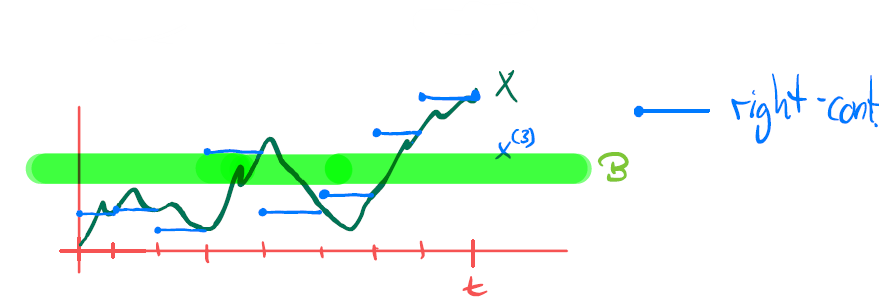
\includegraphics[scale=0.5]{plot28}
%	\end{figure}
%	For any $B \in \varepsilon$ we have
%	\begin{align*}
%		&\{ ( s , \omega ) \in [0,t] \times \Omega | X_s^{(n)}( \omega )\in B \} \\
%		&= \bigcup\limits_{0 \leq k < 2^n}\Bigg(\underbrace{\bigg[\frac{k}{2^n}t,\frac{k+1}{2^n}t\bigg)}_{\in \cB([0,t])}\times \underbrace{\{\omega \colon  X_{\frac{k+1}{2^n}t}\in B \}}_{\in\cF_t} \Bigg)\cup \underbrace{\lbrace t \rbrace}_{\in\cB([0,t])} \times \underbrace{\lbrace \omega \, \colon \, X_t(\omega)\in B \rbrace}_{\in\cF_t}
%	\end{align*}	 
%	$\in \cB\big([0,t]\big) \otimes \cF_t$.
%	By right-continuity $X_s^{(n)}(\omega) \rightarrow X_s(\omega)$ for all $\omega \in \Omega$,\: $s\leq t$. Hence, \:$(s,\omega)\mapsto X_s^{(n)}$ is progressively measurable. Since measurability transfers to point-wise limits, also $(s,\omega) \mapsto X_s$ is progressively measurable.	
%\end{proof}

\begin{ldef}
\begin{deff}\label{def_stopping_time}
	Let $\big(\Omega,\cF,(\cF_n)_{n\in I},\mathbb{P}\big)$ be a filtered probability space.
	\begin{enumerate}[label=(\roman*)]
	\item	 A random variable $\tau\colon \Omega \rightarrow I \cup\lbrace +\infty \rbrace$ is called an \textbf{$(\cF_n)$-stopping time} if
	\[ \lbrace \tau \leq n \rbrace \in \cF_n \quad \forall n \in I \text{.}\]
	\item	$\tau$ is called a \textbf{finite stopping time} if $\tau < \infty $ a.s.
\end{enumerate}
\end{deff}
\end{ldef}
We usually think of a stopping time to model that something of interest happens at that time, for instance a given state is hit by the process. The idea of a stopping time is then easy to grasp: a random variable is called a stoping time if we only need information up to time $n$ to decided if $\tau$ happened before time $n$ or not.

\begin{remark}
	\begin{enumerate}[label=(\roman*)]
		\item It is important to allow $\tau=\infty$ with the interpretation  "{}the thing of interest did not happen"{}.
				\item	Since here we only work in discrete time we could also define a stopping time by asking $\{\tau=n\}\in \mathcal F_n$ for all $n\in I$. This follows easily from
%			\begin{align*}
%				\lbrace \tau < t \rbrace = \bigcup\limits_{n\in\mathbb{N}} \lbrace \tau \leq t-\frac{1}{n} \rbrace \in \cF_t \\
%				\lbrace \tau < t \rbrace = \lbrace \tau \leq t \rbrace \cap \lbrace \tau < t \rbrace^C \in \cF_t
%			\end{align*}
			\begin{align*}
				 \lbrace \tau \leq n \rbrace = \bigcup\limits_{k\leq n}\lbrace \tau = k \rbrace 
			\end{align*}
			because $\lbrace \tau = k \rbrace \in \cF_k \subseteq \cF_n$.
		\item
			A stopping time $\tau$ is not only $\mathcal F$-measurable but even $\cF_{\infty}$-measurable:
			\begin{align*}
				\lbrace \tau =n \rbrace=\lbrace \tau \leq n\}\cap \{\tau \leq n-1\}^C\in \cF_n\subseteq  \cF_{\infty}
			\end{align*}
			and
			\begin{align*}
				\lbrace \tau = \infty \rbrace = \lbrace \tau \neq \infty \rbrace^C = \big( \bigcup\limits_{n\in\mathbb{N}} \lbrace \tau = n \rbrace \big)^C \in \cF_{\infty}.
			\end{align*}	
	\end{enumerate}
\end{remark}
Even though we could formulate everything with $\{\tau =n\}$ we prefer to use $\{\tau \leq n\}$ in order to slowly get acquainted to a notion which cannot be avoided in continuous time.\smallskip


Here are the most important (and most simplistic) examples:
\begin{example}\label{ex_ch2_3}
%	Let $X$ be $(\cF_t)$-adapted.
\begin{lbeispiel}
	\begin{enumerate}[label=(\roman*)]
			\item 
			Every constant $\tau = N$ is a stopping time as $\{N \leq n\}\in \{\emptyset, \Omega\}\in \mathcal F_n$.

		\item
			Fix some $B\in \mathcal E$, then the \textbf{first hitting time} $\tau_B \coloneqq \inf\lbrace n \in I\,:|\, X_n \in B \rbrace$  is a stopping time as
			\begin{align*}
				\lbrace \tau_B \leq n \rbrace = \bigcup\limits_{k\leq n}\underbrace{\lbrace X_k \in B \rbrace}_{\in \mathcal F_k\subseteq \mathcal F_n} \in \cF_n.
			\end{align*}
%		\item 
%			$I = \mathbb{R}_+$,\:$E$ metric space, $\cO \subseteq E$ open,\:$F\subseteq E$ closed
%			\begin{itemize}
%				\item 
%					If $X$ is continuous, then $\tau_F = \inf\lbrace t\leq 0 \colon X_t \in \cO \rbrace$ is an $(\cF_t)$-stopping time
%				\item
%					If $X$ is right-continuous, then $\tau_{\cO} = \inf \lbrace t \geq 0 \colon X_t \in \cO \rbrace$ is an $(\cF_{t+})$-stopping time
%			\end{itemize}			
	\end{enumerate}
\end{lbeispiel}

\end{example}
Intuitively it is clear that the minimum of two stopping times ("{}one of the two events happened"{}) is a stopping time again. Please prove this as a short exercise:
\begin{luebung}
	If $T_1, T_2,...$ is a sequence of $(\cF_n)$-stopping times, then 
	\[ \inf_{k\in\N} T_k , \:\sup_{k\in\N} T_k , \:\liminf_{k\to\infty} T_k, \text{ and }\limsup_{k\to\infty} T_k \]
	are stopping times as well.
\end{luebung}
%\begin{proof}[Proof]
%	Using the definitions of the infimum and limit inferior we can directly check the definition. Fix $n\in I$, then
%	\begin{align*}
%		\{ \inf T_k \leq n \} = \bigcup\limits_{k=1}^{\infty}\underbrace{\{ T_k \leq n \}}_{\in \mathcal F_n}\in \cF_n
%	\end{align*}
%	and
%	\begin{align*}
%		\{ \liminf T_k \leq n \} = \bigcap\limits_{m=0}^{\infty}\bigcup\limits_{k=m}^{\infty}\underbrace{\{T_k \leq n \}}_{\in \cF_n} \in \cF_n.
%	\end{align*}
%	Hence, both are stopping times. For the limit inferior we used that the limit inferior is smaller than $n$ if and only if there are infinitely many $T_k$ which are smaller than $n$ which is equivalent to finding some $T_k$ which are smaller than $n$ after every fixed $m$. \smallskip
%Exercise	
%	The arguments for the supremum and limit superior are similar.
%\end{proof}





As mentioned above we interpret the natural filtration as information of the process, $\mathcal F_n$ as the information up to time $n$. We now generalise towards stopping times and give a mathematical definition of the information up to a stopping time.
\begin{ldef}
\begin{deff}
	Let $\tau$ be an $(\cF_n)$-stopping time. Then
	\begin{align*}
		\cF_{\tau}:= \lbrace A\in \cF_{\infty}\, :\, A \cap \lbrace \tau \leq n \rbrace \in \cF_n \:\: \forall n \in I \rbrace
	\end{align*}
	is called the $\mathbf{\sigma}$\textbf{-algebra generated by $\mathbf{\tau}$}
\end{deff}
\end{ldef}
It will need a bit of time to get used to $\mathcal F_\tau$. As always it is most instructive to have some examples in mind. Fix the first stopping time $\tau_B$ of a set $B$ and check by hands that for some other set $A$ the event "{}$A$ was hit before $B$"{} is in $\mathcal F_{\tau_{B}}$. This should intuitively be clear as only the process until first hitting $B$ is needed to decide if $A$ was already hit. 
\begin{llemma}
\begin{prop}\label{ii}
	Suppose $\tau$ is an $(\mathcal F_n)$-stopping time. 
	\begin{enumerate}[label=(\roman*)]
		\item 	$\cF_{\tau}$ is a $\sigma$-algebra on $\Omega$.
		\item	 	$\tau$ is $\cF_{\tau}$-measurable.
	\end{enumerate}
\end{prop}
\end{llemma}
\begin{proof}[Proof]
\begin{enumerate}[label=(\roman*)]
\item Let us check the defining properties of a $\sigma$-algebra:
	\begin{itemize}
		\item
			$\Omega \cap \lbrace \tau \leq n \rbrace \in \cF_n$, hence, $\Omega \in \mathcal F_\tau$.
		\item
			Let $A \in \cF_{\tau}$, then \[ A^C \cap \lbrace \tau \leq n \rbrace = \lbrace \tau \leq n \rbrace \cap \big( A \cap \lbrace \tau \leq n \rbrace \big)^C \in \cF_n \]
			so that $A^C\in \cF_\tau$.		
		\item
			Let $A_1,A_2,... \in \cF_{\tau}$, then
				\[ \bigcup\limits_{k=1}^{\infty}A_k \: \cap \lbrace \tau \leq n \rbrace = \bigcup\limits_{k=1}^{\infty} \underbrace{\left(A_k \cap \lbrace \tau \leq n \rbrace\right)}_{\in \cF_n}\in\cF_n \]
			so that $\cup_{k=1}^\infty A_k\in \mathcal F_\tau$.
	\end{itemize}
\item Exercise

\end{enumerate}
\end{proof}

Stopping times are useful as many properties of deterministic times also hold for stopping times.
\begin{llemma}
\begin{prop}\label{pS}
	Suppose $S, T$ are $(\cF_n)$-stopping times.
	\begin{enumerate}[label=(\roman*)]
		\item
			$S \leq T$\, a.s.\, $\Rightarrow\,$ $\cF_S \subseteq \cF_T$
		\item
			$\cF_{S\wedge T} = \cF_S \cap \cF_T$
		\item
			$\lbrace S \leq T \rbrace \in \cF_{S\wedge T}$ and $\lbrace S = T \rbrace \in \cF_{S\wedge T}$
%		\item
%			$S+T$ is an $(\cF_n)$-stopping time
	\end{enumerate}
\end{prop}
\end{llemma}
Before checking the proofs have a quick thought why those statements should intuitively be true with the interpretation of stopping times and the information given by a stopping time.
\begin{proof}[Proof]
	\begin{enumerate}[label=(\roman*)]
		\item
			\begin{align*}
				A \in \cF_S \quad &\Rightarrow \quad A \cap \lbrace S\leq n \rbrace \in \cF_n\,\, \forall n \in I \\
							&\Rightarrow \quad A \cap \lbrace T \leq n \rbrace = A \cap \lbrace S \leq n \rbrace \cap \lbrace T \leq n \rbrace \in \cF_n\,\,\forall n \in I\\
							&\Rightarrow  \quad A \in \cF_{T}
			\end{align*}
		\item We have seen above that $S\wedge T$ is an $(\mathcal F_n)$-stopping time again. Now towards the generalised $\sigma$-algebras:\smallskip
			
			"$\supseteq$": Let $A\in \cF_S\cap\cF_T$ and $n\in I$, then 
					\[ A \cap \{ S \wedge T \leq n \} = A \cap \big( \{ S \leq n \} \cup \{ T \leq n \} \big) =\big(A \cap  \{ S \leq n \} \big) \cup \big( A\cap \{ T \leq n \} \big) \in \cF_n \]
					Hence, $A \in \cF_{S\wedge T}$.\smallskip
				
			"$\subseteq$": This follows from the monotonicity proved in (i): $\cF_{S\wedge T} \subseteq \cF_s$, $\cF_{S\wedge T} \subseteq \cF_T$
		\item	Try yourself!		
	\end{enumerate}
\end{proof}
The definitions of stopping times and adapted processes work nicely together, here is an example:
\begin{llemma}
\begin{prop}\label{cha2_prop_X_tau_adapted}
	If $X$ is adapted to the filtration $(\cF_n)$ and $\tau$ is a finite $(\mathcal F_n)$-stopping time, then $X_{\tau}$ is $\cF_{\tau}$-measurable.
\end{prop}
\end{llemma}
\begin{proof}[Proof]
	The finiteness of $\tau$ was only assumed to make $X_\tau$ well-defined as we did not define $X_\infty$. Let $A \in \mathcal{E}$, we show $\lbrace X_{\tau} \in A \rbrace \in \cF_{\tau}$. Let $n\in I$, then
	\begin{align*}
		\lbrace X_{\tau} \in A \rbrace \cap \lbrace \tau \leq n \rbrace = \bigcup_{m\leq n}\underbrace{ \{ X_m \in A \} \cap \{ \tau = m \} }_{\in \mathcal F_m \subseteq \mathcal F_n}\in \cF_n
	\end{align*}
\end{proof}


	\marginpar{\textcolor{red}{Lecture 5}}
\section{Basics of martingales}

All processes in this chapter are indexed by discrete ordered sets such as $I = \mathbb{N}_0$, $I =\mathbb{N}$, $I=\Z$, $I=-\N$, or $I \subseteq \mathbb{N}$ and we write $n$ instead of $t$. We start the discussion of martingales with definitions and some first properties.

\begin{ldef}
\begin{deff}\label{def_martingale}
Let $I$ a discrete ordered index-set, $\big(\Omega , \cF , (\cF_n)_{n\in I}, \mathbb{P}\big)$ a filtered probability space, and $X=(X_n)_{n\in I}$ an $(\cF_n)_{n\in I}$-adapted process with $\E[\left| X_n \right| ] < \infty$ for all $ n \in I$. Then $X$ is called an
	\begin{enumerate}[label=(\roman*)]
		\item 
			$(\cF_n)_{n\in I}$\textbf{-martingale} if $\E[X_{n+1}\,|\,\cF_n]=X_n$ a.s. for all $n\in I$,
		\item
			$(\cF_n)_{n\in I}$\textbf{-supermartingale} if $\E[X_{n+1}\,|\,\cF_n] \leq X_n$ a.s. for all $ n\in I$,
		\item
			$(\cF_n)_{n\in I}$\textbf{-submartingale} if $\E[X_{n+1}\,|\,\cF_n] \geq X_n$ a.s. for all $ n\in I$.
	\end{enumerate}
	If $I=-\N$ or $I=-\N_0$ we will speak of a \textbf{backwards martingale}, for $I=\N$, $I=\N_0$, or $I=\{0,...,N\}$ of a \textbf{forwards martingale} but we will always skip the supplement forwards.
\end{deff}
\end{ldef}
The interpretation of a martingale is that of a fair game (this is where the name "{}martingale"{} comes from). Given the past value the expectation of profit in the next step is $0$. Analogously, a supermartingale is seen as an unfavourable game (we will loose in expectation) and submartingales are seen as favourable games. The power of martingales is astonishing. Most of the time they appear from nowhere in a context that does not look like a typical martingale setting and their powerful convergence theorems yield strong results. We will see as an example a proof of the law of large numbers without any additional assumption.\smallskip

Please check the following easy properties yourself!
\begin{luebung} 
	\begin{enumerate}[label=(\roman*)]
		\item The (sub)(super)martingale property also holds over several time steps:
		\begin{align*}
		 \E[X_m \, |\,\cF_n]\,\,
		\begin{cases}
			=X_n&: X\text{ martingale}\\
			\leq X_n&: X\text{ supermartingale}\\
			\geq X_n&: X\text{ supermartingale}
			\end{cases},
		\end{align*}
		for all $m\geq n$.
%			Why?
%			\begin{align*}
%				\E[X_m \,|\, \cF_n] &= \E \big[ \E [ X_m \, | \, \cF_{m-1}]\, | \, \cF_n \big] && \text{tower property}\\
%				&=\E[X_{m-1}\,|\,\cF_n] \\
%				&= ...&& \text{turn this into an induction!} \\
%				&= \E[X_{n+1}\,|\, \cF_n] = X_n
%			\end{align*}
		\item	Expectations (increase)(decrease)stay constant depending on $X$ being a (sub)(super)martingale:
		\begin{align*}
			\E[X_m] \,\,
			\begin{cases}
				=\E[X_n]&: X\text{ martingale}\\
				\leq \E[X_n]&:X\text{ supermartingale}\\
				\geq \E[X_n]&:X\text{ submartingale}\\				
			\end{cases},
		\end{align*}	
		for all $m\geq n$.
%			$\E[X_m] = \E[X_n], m \geq n$, if $(X_n)_{n\in\mathbb{N}}$ is a martingale, \\
%			$\E[X_m] \leq \E[X_n], m \geq n$, if $(X_n)_{n\in\mathbb{N}}$ is a supermartingale and \\
%			$\E[X_m] \geq \E[X_n], m \geq n$, if $(X_n)_{n\in\mathbb{N}}$ is a submartingale \\
%			Why? $\E[X_n] = \E \big[ \E[X_m\,|\,\cF_n] \big] = \E[X_m]$
		
		\item
			$X$ is a supermartingale $\Leftrightarrow$ $-X$ is a submartingale.
	\end{enumerate}
\end{luebung}
The final property allows us to prove theorems in most cases for either sub- or supermartingales and then transfer the theorems to the other.\smallskip

Even though the (super)(sub)martingale properties seems artificial many stochastic processes share this property:
\begin{example}\label{ex:RW}
	The most prominent stochastic process in discrete time is the random walk which is a Markov chain and also a martingale.
	
\begin{figure}[h]
\begin{center}
\scalebox{0.8}{
  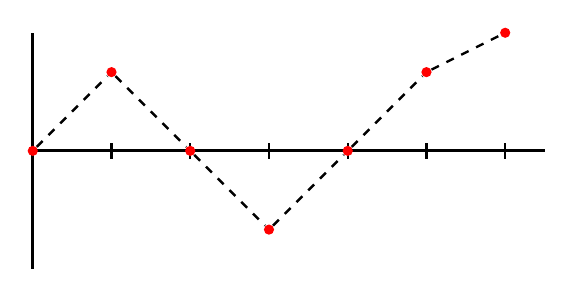
\begin{tikzpicture}
  \tikzset{
    pics/tick/.style args={#1}{code={
      \draw[line width=0.3mm] (0,-#1) -- (0,#1) ;
      },
    }
  }
    %AXIS Y
    \draw[line width=0.4mm] (0,-1.5) -- ++(90:3cm);
    %AXIS X 
    \draw[line width=0.4mm] (0,0) --++(0:6.5cm);

    \draw (0,0) pic {tick={1mm}} node[circle,inner sep=1.3pt,fill=red,yshift=0cm] (0) {};
    \draw (1,0) pic {tick={1mm}} node[circle,inner sep=1.3pt,fill=red,yshift=1cm] (1) {};
    \draw (2,0) pic {tick={1mm}} node[circle,inner sep=1.3pt,fill=red,yshift=0] (2) {};
    \draw (3,0) pic {tick={1mm}} node[circle,inner sep=1.3pt,fill=red,yshift=-1cm] (3) {};
    \draw (4,0) pic {tick={1mm}} node[circle,inner sep=1.3pt,fill=red,yshift=0cm]  (4) {};
    \draw (5,0) pic {tick={1mm}} node[circle,inner sep=1.3pt,fill=red,yshift=1cm] (5) {};
    \draw (6,0) pic {tick={1mm}} node[circle,inner sep=1.3pt,fill=red,yshift=1.5cm] (6) {};
    \foreach \x/\y in {0/1,1/2,2/3,3/4,4/5,5/6} {
      \draw[dashed,line width=0.3mm] (\x) -- (\y) ;
    }
  \end{tikzpicture} 
  }
  \end{center}
  \vspace{-4mm}
  \caption*{A trajectory of the simple random walk}
\end{figure}
	\begin{lbeispiel}		
	Let $Y_1,Y_2,Y_3,..$ be iid real-valued integrable random variable on some probability space $(\Omega, \mathcal A, \P)$. The \textbf{random walk with jump sizes $Y_k$} is defined by $X_0:=x\in\R$ and 
			\begin{align*}
			 	X_n = x + \sum\limits_{k=1}^{n}Y_k, \quad n \in \mathbb{N}.
			\end{align*}
					If $\P(Y_1=1)=p$ and $\P(Y_1=-1)=1-p$ the random walk is called \textbf{simple random walk}, for $p=\frac 1 2$ symmetric simple random walk.
		\end{lbeispiel}
				\vspace{-2mm}

		
			If we define $\cF_0 = \lbrace \emptyset,\Omega \rbrace$ and $\cF_n = \sigma(Y_1,...,Y_n)$ then the random walk is an
			\begin{itemize}
				\item
					$(\mathcal F_n)$-martingale if $\E[Y_1]=0$,
				\item
					$(\mathcal F_n)$-supermartingale if $\E[Y_1] \leq 0$,
				\item
					$(\mathcal F_n)$-submartingale if $\E[Y_1] \geq 0$.
			\end{itemize}
			To see why, let us check the definition. Adaptivity and integrability ($\Delta$-inequality) is clear, the martingale property is deduced using properties of the conditional expectation:
			\begin{align*}
				\E[X_{n+1}\,|\,\cF_n] &= \E \big[ \sum\limits_{k=1}^{n+1}Y_k \,\big|\,\cF_n\big]\\
											&= \sum\limits_{k=1}^{n+1} \E[Y_k\,|\,\cF_n] \\
											&= \sum\limits_{k=1}^{n}Y_k \: + \: \E[Y_{n+1}\,|\,\cF_n]\\% && Y_k\:\text{is}\: \cF_n\text{-meas. for}\: k\leq n \\
											&= X_n + \E[Y_1],
			\end{align*}
			using in the third equality the measurability and independence assumption on the jump sizes.
\end{example}
\begin{example}\label{GW}		
 Another famous class of discrete time stochastic processes are so-called branching processes ("{}Verzweigungsprozesse"{}). 
\begin{lbeispiel}
	Let $\xi_i^n,\: i,n\in \mathbb{N}$, be integrable, non-negative discrete iid random variables with $\mathbb{P}(\xi_1^n=k) = p_k$, $k\in\mathbb{N}_0$. 
	The classical \textbf{branching process} (or \textbf{Galton-Watson process}) with offspring distribution $\xi$ is defined by
	\begin{align*}
		X_0 &\coloneqq m,\quad	X_{n+1} \coloneqq \sum_{k=1}^{X_n}\xi_k^n,\quad n\in\N.
	\end{align*}
	We will call $X_n$ the number of individuals of a population at time $n$.
\end{lbeispiel}

\begin{figure}[h]
	\begin{center}
	\raisebox{-1cm}{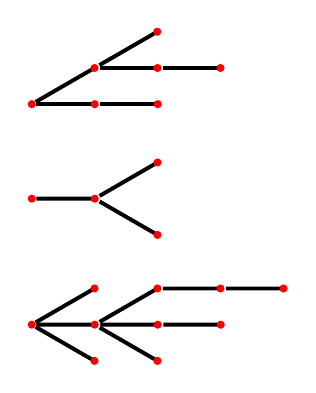
\begin{tikzpicture}[scale=0.8,transform shape]
	%TREE 1 LEVEL 1
	\node [circle,inner sep=1.3pt,fill=red] (L11) at (0,0) {};
	  %LEVEL 2
	  \draw[line width=0.5mm] (L11) -- ++(0:10mm) node [circle,inner sep=1.3pt,fill=red] (L21)  {};
	  \draw[line width=0.5mm] (L11) -- ++(30:11.5mm) node [circle,inner sep=1.3pt,fill=red] (L22)  {};
	  %LEVEL 3 
		\draw[line width=0.5mm] (L22) -- ++(-0:10mm) node [circle,inner sep=1.3pt,fill=red] (L31)  {};
		\draw[line width=0.5mm] (L22) -- ++(30:11.5mm) node [circle,inner sep=1.3pt,fill=red] (L32)  {};
		%LEVEL 4 
		  \draw[line width=0.5mm] (L31) -- ++(0:10mm) node [circle,inner sep=1.3pt,fill=red] (L41)  {};
  
		\draw[line width=0.5mm] (L21) -- ++(0:10mm) node [circle,inner sep=1.3pt,fill=red] (L33)  {};
  
	%TREE 2 LEVEL 1
	\node [circle,inner sep=1.3pt,fill=red] (L11) at (0,-1.5) {};
	  %LEVEL 2
	  \draw[line width=0.5mm] (L11) -- ++(0:10mm) node [circle,inner sep=1.3pt,fill=red] (L21)  {};
	  %LEVEL 3 
		\draw[line width=0.5mm] (L21) -- ++(-30:11.5mm) node [circle,inner sep=1.3pt,fill=red] (L31)  {};
		\draw[line width=0.5mm] (L21) -- ++(30:11.5mm) node [circle,inner sep=1.3pt,fill=red] (L32)  {};
  
  
	%TREE 3 LEVEL 1
	\node [circle,inner sep=1.3pt,fill=red] (L11) at (0,-3.5) {};
	  %LEVEL 2
	  \draw[line width=0.5mm] (L11) -- ++(0:10mm) node [circle,inner sep=1.3pt,fill=red] (L21)  {};
	  \draw[line width=0.5mm] (L11) -- ++(30:11.5mm) node [circle,inner sep=1.3pt,fill=red] (L22)  {};
	  \draw[line width=0.5mm] (L11) -- ++(-30:11.5mm) node [circle,inner sep=1.3pt,fill=red] (L23)  {};
	  %LEVEL 3 
		\draw[line width=0.5mm] (L21) -- ++(-0:10mm) node [circle,inner sep=1.3pt,fill=red] (L31)  {};
		\draw[line width=0.5mm] (L21) -- ++(30:11.5mm) node [circle,inner sep=1.3pt,fill=red] (L32)  {};
		\draw[line width=0.5mm] (L21) -- ++(-30:11.5mm) node [circle,inner sep=1.3pt,fill=red] (L33)  {};
		%LEVEL 4 
		  \draw[line width=0.5mm] (L32) -- ++(0:10mm) node [circle,inner sep=1.3pt,fill=red] (L41)  {};
		  \draw[line width=0.5mm] (L31) -- ++(0:10mm) node [circle,inner sep=1.3pt,fill=red] (L42)  {};
		  %LEVEL 5
			\draw[line width=0.5mm] (L41) -- ++(0:10mm) node [circle,inner sep=1.3pt,fill=red] (L51)  {};       
	\end{tikzpicture}}
	\hspace{1cm}
	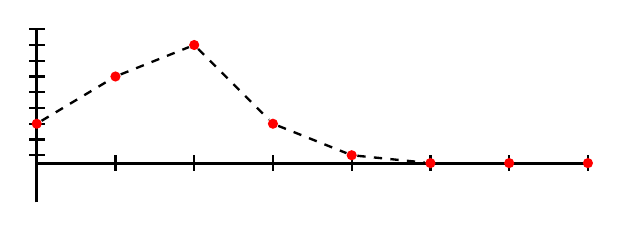
\begin{tikzpicture}
	\tikzset{
	  pics/tick/.style args={#1}{code={
		\draw[line width=0.3mm] (0,-#1) -- (0,#1) ;
		},
	  }
	}
	%AXIS Y
	\draw[line width=0.4mm] (0,-0.5) -- ++(90:2.2cm);
	%AXIS X 
	\draw[line width=0.4mm] (0,0) --++(0:7cm); 
	%YTICKS 
	\foreach \y in {0.1,0.3,...,1.7}{
	  \draw[] (0,\y) pic[rotate=90] {tick={1mm}};
	} 
	\draw (0,0) pic {tick={1mm}} node[circle,inner sep=1.3pt,fill=red] (0) at (0,0.5){};
	\draw (1,0) pic {tick={1mm}} node[circle,inner sep=1.3pt,fill=red] (1) at (1,1.1){};
	\draw (2,0) pic {tick={1mm}} node[circle,inner sep=1.3pt,fill=red] (2) at (2,1.5){};
	\draw (3,0) pic {tick={1mm}} node[circle,inner sep=1.3pt,fill=red] (3) at (3,0.5){};
	\draw (4,0) pic {tick={1mm}} node[circle,inner sep=1.3pt,fill=red] (4) at (4,0.1){};
	\draw (5,0) pic {tick={1mm}} node[circle,inner sep=1.3pt,fill=red] (5) at (5,0)  {};
	\draw (6,0) pic {tick={1mm}} node[circle,inner sep=1.3pt,fill=red] (6) at (6,0)  {};
	\draw (7,0) pic {tick={1mm}} node[circle,inner sep=1.3pt,fill=red] (7) at (7,0)  {};
	\foreach \x/\y in {0/1,1/2,2/3,3/4,4/5,5/6,6/7} {
		\draw[dashed,line width=0.3mm] (\x) -- (\y) ;
	  }
	\end{tikzpicture}
	  %raisebox adjusts text height  
	 \raisebox{-1cm}{\hspace{10mm} Branching process with m=3 and extinction time 5}
\end{center}
  \end{figure}\footnote{y-achse stimmt nicht ganz}

	The interpretation goes as follows. At time zero there are $m$ individuals, plants for examples. At every time-unit, once a year for plants, every existing individual gets a random number of offspring. The number is independent from all offspring of other individuals in the same generation but also independent of the past. The genealogical picture is typically represented by a graph, $X_n$ counts the number of individuals at time $n$. We say the branching process gets extinct if $X_n=0$, after the first extinction time the process stays extinct forever. We always assume $p_0,p_1\neq 1$ as otherwise the branching process either dies out immediately ($p_0=1$ forces all initial individuals to have zero offspring) or stays constant ($p_1=1$ forces all individuals to have exactly one offspring so that $X_n=m$ for all $n\in\N$). Typical questions concern the probability of extinction or the rate of growth (exponential, subexponential). A critical feature is the mean number of offspring $\mu =\E[\xi_1^n] = \sum_{k=0}^{\infty}k\cdot p_k$ which is the main driver for the longtime behavior.\smallskip
	
	 If we define $\cF_0 = \lbrace \emptyset,\Omega \rbrace$ and $\cF_n = \sigma(\xi_i^k: i\in \N,k\leq n)$ then the branching process $X$ is an
			\begin{itemize}
				\item
					$(\mathcal F_n)$-martingale if $\mu=1$, called the \textbf{critical case},
				\item
					$(\mathcal F_n)$-supermartingale if $\mu<1$, called the \textbf{subcritical case},
				\item
					$(\mathcal F_n)$-submartingale if $\mu>1$, called the \textbf{supercritical case}.
			\end{itemize}
	Let us check the definition which is similar to the computation for the random walk except we need to deal with the random delimiter in the sums for which we need the Wald-identity:
	\begin{luebung}
		Suppose $N, Y_1,Y_2,...$ are independent, $\E[N]<\infty$, and $Y_1,Y_2,...$ are identically distributed, then
		\begin{align}\label{Wald}
			\E\Big[\sum_{k=1}^N Y_k\Big]=\E[N]\cdot \E[Y_1].
		\end{align}
	\end{luebung}
	Integrability is deduced immediately as the Wald-identity gives $\E[X_n]=\E[X_{n-1}]\cdot \E[\xi_1^1]$ so that $\E[X_n]=m\mu^{n}<\infty$ by a simple induction. Adaptivity follows direction from the definition of $\mathcal F_n$. The martingale property is deduced using properties of the conditional expectation:
			\begin{align*}
				\E[X_{n+1}\,|\,\cF_n] &= \E\big[ \sum_{k=1}^{\infty}\mathbf 1_{k \leq X_n}\cdot \xi_k^{n+1}\,\big|\,\cF_n\big] \\
										&=\sum_{i=1}^{\infty}\mathbf 1_{j \leq X_n} \E\big[\xi_j^{n+1}\,|\,\cF_n\big] \\
										&=\sum_{i=1}^{\infty}\mathbf 1_{j \leq X_n} \E\big[\xi_j^{n+1}\big] 
										=\mu \cdot X_n,
			\end{align*}
			using monotone convergence, measurability and the independence of conditional expectation. Interestingly, there is another martingale appearing in the branching process. If we define $M_n \coloneqq \frac{1}{\mu^n}\cdot X_n$, $n\in\N$, then $M$ is a martingale in all three regimes! Adaptivity and measurability is clear, the martingale property follows with the same calculation as above with an additional cancellation:			
			$$ \E[M_{n+1}\,|\,\cF_n] = \frac{1}{\mu^{n+1}}\cdot \E[X_{n+1}\,|\,\cF_n] = \frac{1}{\mu^{n+1}} \cdot \mu \cdot X_n = M_n.$$
			We already get a first impression of what is going by checking the expectations, which are constant for the martingale $M$. Then the expectations of $X_n$ remain constant for $\mu=1$ grow exponentially as $\mu^n=e^{\log(\mu)n}$ for $\mu>1$ and decay exponentially for $\mu<1$.
		\end{example}
\begin{example}\label{doobmartingale}
%\begin{enumerate}
%	\item
%			If $(X_n)_{n\in \mathbb{N}}$ is a generic integrable, $(\cF_n)$-adapted, decreasing (i.e. $X_n \geq X_{n+1}$ a.s.) process, then $(X_n)_{n\in\mathbb{N}}$ is an $(\cF_n)$-supermartingale as
%			\begin{align*}
%				 \E[X_{n+1}\,|\,\cF_n] \leq \E[X_n\,|\,\cF_n] = X_n \quad \text{a.s.}
%			\end{align*}
%			Similarly, an adapted increasing process is a submartingale.
%		\item
			If $Z$ is an integrable random variable on $(\Omega,\cF,\mathbb{P})$ and $(\cF_n)$ is a filtration, then $$X_n \coloneqq \E[Z\,|\,\cF_n],\quad n\in\N,$$ is a martingale. The argument is simple but very important:
			\begin{align*}
				\E[X_{n+1}\,|\,\cF_{n}] = \E \big[ \E[Z\,|\,\cF_{n+1}]\,\big|\,\cF_n \big] 
											\overset{\text{tower prop.}}{=} \E[Z\,|\,\cF_n] = X_n\quad \text{a.s.}
			\end{align*}
			Every martingale $(X_n)_{n\in\mathbb{N}}$ that can be written as $\E[Z\,|\,\cF_n]$ for some integrable random variable $Z$ is called a \textbf{closed martingale} or \textbf{Doob martingale}. It is best to think of a Doob martingale as a martingale on finite time horizon $\{0,...,N\}$ as in both cases one random variable ($Z$ for a Doob martinglae, $X_N$ for a finite-time martingale) determines the entire martingale. In the end of Section \ref{secL1} it will be shown that closed martingales (or, equivalently, uniformly integrable martingales) indeed share important properties of finite-time martingales.
%			
%			
%			We will think of $Z$ as the last element as we will later see the connection to the limit $X_\infty=\lim_{n\to\infty} X_n$. Doob martingales are useful as only one random variable $Z$ determines all random variables $X_n$, in a way, closed martingales are as simple as martingales on finite time-horizon $\{0,...,N\}$. It will be proved later that many martingales are Doob martingales!
%	\end{enumerate}

	\end{example}
\begin{llemma}
\begin{prop}\label{prop314}
	Let $\varphi \colon \mathbb{R} \rightarrow \mathbb{R}$ be a convex function, and $(X_n)_{n\in\mathbb{N}}$ a stochastic process with $\E[\left| \varphi(X_n)\right|] < \infty$.
	\begin{enumerate}[label=(\roman*)]
		\item
			If $(X_n)_{n\in\mathbb{N}}$ is an $(\cF_n)$-martingale, then $\big(\varphi(X_n)\big)_{n\in\mathbb{N}}$ is an $(\cF_n)$-submartingale.
			
		\item
			If $(X_n)_{n\in\mathbb{N}}$ is an $(\cF_n)$-submartingale and $\varphi$ is increasing, then $\big(\varphi(X_n)\big)_{n\in\mathbb{N}}$ is an $(\cF_n)$-submartingale.
	\end{enumerate}
\end{prop}
\end{llemma}
\begin{proof}
	We use Jensen's inequality for conditional expectation:
	\begin{enumerate}[label=(\roman*)]
		\item
			$\E \big[\varphi(X_{n+1})\,|\,\cF_n\big] \geq \varphi \big( \E[X_{n+1}\,|\,\cF_n]\big) = \varphi(X_n)$ a.s. The equality uses the martingale property.
		\item
			$\E \big[\varphi(X_{n+1})\,|\,\cF_n\big] \geq \varphi \big( \E[X_{n+1}\,|\,\cF_n]\big) \geq \varphi (X_n)$ a.s. The second inequality uses that $\varphi$ is increasing and the submartingale property.
	\end{enumerate}
\end{proof}
As usual, the simplest examples are the most useful ones. One can regularly see the use of $\varphi (x) = \left| x \right|$, $\varphi (x) = (x-a)^+ $, and powers $\varphi (x) = \left| x \right|^p$ for $p \geq 1$.
\begin{lwarnhinweis}
	Most importantly, $(X_n^2)_{n\in\N}$ is a submartingale if $(X_n)_{n\in\mathbb{N}}$ is a martingale with $\E[X_n^2]<\infty$ for all $n\in\N$.
\end{lwarnhinweis}
Here is something simple to check yourself. 
\begin{luebung}
	Suppose $(X_n)_{n\in\mathbb{N}}$ and $(Y_n)_{n\in\mathbb{N}}$ are $(\cF_n)$-martingales.
	Then the sum $(X_n+Y_n)_{n\in\mathbb{N}}$ is an $(\cF_n)$-martingale and the maximum $(X_n \vee Y_n)_{n\in\mathbb{N}}$ is an $(\cF_n)$-submartgingale.
\end{luebung}
%\begin{proof}
%$\E[X_{n+1}+Y_{n+1} \, | \, \cF_n ] = \E[X_{n+1}\,|\,\cF_n]+\E[Y_{n+1}\,|\,\cF_n] \geq X_n + Y_n$ a.s.\\
%$\E[X_{n+1}\vee Y_{n+1}\,|\,\cF_n] \geq \E[X_{n+1}\,|\,\cF_n] \geq X_n$ a.s. and \\
 %$\E[X_{n+1}\vee Y_{n+1}\,|\,\cF_n] \geq \E[Y_{n+1}\,|\,\cF_n] \geq Y_n$.\\ Hence, $\E[X_{n+1}\vee Y_{n+1}\,|\,\cF_n] \geq X_{n+1}\vee Y_{n+1}$ a.s.
%\end{proof}
We come to the first theorem on martingales where we relate martingales and stopping times. If $T$ is a stopping time then we define the \textbf{stopped process} $X^T$ as $$X_n^T(\omega)\coloneqq X_{n \wedge T(\omega)}(\omega),\quad n \in \mathbb{N}.$$ The path of the stopped process is the same as the original process up to time $T$ and stays constant at the value $X_T$ after time $T$. 
\begin{figure}[h]
  \begin{center}
  \scalebox{0.7}{
  \begin{tikzpicture}
  \tikzset{
    cross/.pic ={
      \draw[pic actions,rotate=#1,line width=0.3mm] 
        (-3pt,0) -- (3pt,0)
        (0,-3pt) -- (0,3pt);
    },
  }
  \tikzset{
    pics/tick/.style args={#1}{code={
      \draw[line width=0.3mm] (0,-#1) -- (0,#1) ;
      },
    }
  }
  %AXIS Y
  \draw[black,line width=0.4mm] (0,-0.5) -- ++(90:4.5cm);
  %AXIS X 
  \draw[black,line width=0.4mm] (-0.5,0) --++(0:9cm); 
  \foreach \x in {1,2,...,8}{
    \draw (\x,0) pic {tick={1mm}} ;
  }
  \foreach \x/\y in {1/1,2/2,3/1.5,4/2.5,5/2}{
    \draw (\x,\y) pic {cross={0}} node[inner sep=0mm] (\x) {};
    \draw[violet] (\x,\y) pic {cross={45}};
  }
  \draw[violet] (5,0) pic {tick={1mm}};

  
  \definecolor{darkViolet}{RGB}{74,2,104}
  \draw[violet] (6,2) pic {cross={45}} node[] (6) {} ;
  \draw[violet] (7,2) pic {cross={45}} node[] (7) {};
  \draw[violet] (8,2) pic {cross={45}} node[] (8) {};

  \foreach \x/\y in {0/1,1/2,2/3,3/4,4/5,5/6,6/7,7/8} {
      \draw[dashed,line width=0.2mm,draw=darkViolet] (\x) -- (\y) ;
    }

  \draw (6,3)   pic {cross={0}}node[inner sep=0.5mm] (6) {};
  \draw (7,2.5) pic {cross={0}}node[inner sep=0.5mm] (7) {};
  \draw (8,3.5) pic {cross={0}}node[inner sep=0.5mm] (8) {};

  \draw[dashed,line width=0.2mm,draw=black] (5) -- (6) ;
  \draw[dashed,line width=0.2mm,draw=black] (6) -- (7) ;
  \draw[dashed,line width=0.2mm,draw=black] (7) -- (8) ;


  %TEXT 
  \node[violet,yshift=-4mm] (stopT) at (5,0) {$T$};

  \node[black] (blackPath) at  (9,3.5) {$X$} ;
  \node[violet,yshift=-4mm,xshift=1mm] (violetPath) at (blackPath.south)  {$X^T$};
  \end{tikzpicture}
  }
\vspace{-2mm}
\caption*{Path of a stopped process $X^T$}
\end{center}
\end{figure}
It might be instructive to realise that stopping at deterministic times $T=N$ shows how to relate infinite time-horizon martingales to finite time-horizon martingales on $\{0,...,N\}$.\smallskip

The optional stopping theorem states that a martingale stopped at a stopping time (i.e. without future information) remains a martingale. We can derive as an application the so-called optional sampling theorem. The theorem formalises the idea of a fair game that without future information it is impossible to reach a gain in expectation by stopping. While we will see after the theorem an example that this statement is a bit too optimistic it does hold for bounded stopping times:
\begin{lsatzwichtig}
\begin{theorem}[Optional Stopping/Optional Sampling Theorem]\label{optional_stopping}
	Suppose $(X_n)_{n\in\mathbb{N}}$ is an $(\cF_n)$-martingale and $T$ is an $(\cF_n)$-stopping time.
	\begin{enumerate}[label=(\roman*)]
		\item The \textbf{stopped process} $(X_n^T)_{n\in\N}$ is an $(\cF_n)$-martingale.
		\item
			If $T$ is a \textbf{bounded} $(\cF_n)$-stopping time, i.e. $\mathbb{P}(T \leq K ) = 1$ for some $K\in \mathbb{N}$, then $X_T$ is an integrable random variable with $\E[X_T] = \E[X_1]$.
	\end{enumerate}
\end{theorem}
\end{lsatzwichtig}
The optional sampling theorem in particular applies to martingales on finite time-horizon $\{0,...,N\}$ when the optional sampling theorem is applied to the stopped martingale $X^N$.



\begin{proof}[Proof]
	We mainly prove the optional stopping theorem, optional sampling is a direct consequence.\smallskip
	
	\textbf{Optional Stopping Theorem:} 
			We check the three defining properties (adapted, integrable, martingale property):
			\begin{itemize}\label{(i)}
				\item 
					First note that $n\wedge T$ is a stopping time (minimum of two stopping times), hence, $X_{n\wedge T}$ is $\cF_{n \wedge T}$-measurable by Proposition \ref{cha2_prop_X_tau_adapted}. Since $\cF_{n\wedge T} \subseteq \cF_n$ by Proposition \ref{pS}, $X^T$ is $(\cF_n)$-adapted.
				\item The integrability of $X^T$ follows by splitting on the possible values of $T$:
				\begin{align*}
						\E\big[| X_n^T |\big] &= \E \Big[ \left| X_{n \wedge T} \right|  \sum\limits_{k=1}^{\infty}\mathbf 1_{T=k} \Big]\\
						&\leq \E \Big[\sum\limits_{k=1}^{n} \left| X_{k} \right|  \mathbf 1_{T=k} \Big]+\E \Big[\sum\limits_{k={n+1}}^{\infty } \left| X_{n} \right|  \mathbf 1_{T=k} \Big]\\				
						&\leq \E \Big[\sum\limits_{k=1}^{n} \left| X_{k} \right| \Big]+\E \big[\left| X_{n} \right| \mathbf 1_{T\geq n+1}\big]\\				
						&\leq \sum\limits_{k=1}^{n} \E [| X_{k} | ]+\E [\left| X_{n} \right| ]<\infty.
				\end{align*}					
				\item To show the martingale property we use a trick that will return frequently. To show the martingale property it is enough to show that the differences are so-called martingale differences:
				\begin{ltippwichtig}
					Trick: $(X_n)_{n\in\mathbb{N}}$ is an $(\cF_n)$-martingale iff $\E[X_{n+1}-X_n\,|\,\cF_n]=0$ a.s. for all $n\in\N$. 
				\end{ltippwichtig}
				To justify the martingale difference trick one only needs to use the linearity of conditional expectation and that $X$ is adapted.\smallskip
				
				Let's check that the differences of $X^T$ are martingale differences:
					\begin{align*}
						\E\big[X_{n+1}^T-X_n^T\,\big|\,\cF_n\big] &= \E \big[ (X^T_{n+1}-X^T_n)(\mathbf 1_{T\leq n}+\mathbf 1_{T > n})\,\big|\,\cF_n\big] \\
						&= \E\big[(X_{n+1}-X_n) \mathbf 1_{T > n}\,\big|\,\cF_n\big] \\
						&= \mathbf 1_{T>n} \E[X_{n+1}-X_n\,|\,\cF_n] 
						= 0
					\end{align*}
					where we used that
					\begin{itemize}
						\item
							$X_{n+1}^T=X_n^T$ on the event $\lbrace T \leq n \rbrace$,
						\item
							$X_{n+1}^T = X_{n+1}, X_n^T = X_n$ on $\lbrace T > n \rbrace$,
						\item
							$\mathbf 1_{T>n}$ is measurable as $\lbrace T>n \rbrace = \lbrace T\leq n\rbrace^C \in \cF_n$ by the stopping time property.
					\end{itemize}
			\end{itemize}
			
			\textbf{Optional Sampling Theorem:} 
			Using that the stopped martingale is again a martingale and that martingales have constant expectations we obtain the theorem:
			\begin{align*}
				\E[X_T] \overset{T\leq K}{=} \E[X_{K\wedge T}] =\E[X_{K}^T]=\E[X_1^T] = \E[X_{T \wedge 1}] = \E[X_1].
			\end{align*}				
\end{proof}
\begin{lwarnhinweis}
	The boundedness of $T$ can be weakend but not generally be removed! Always keep in mind the random walk example below as a counter example!
\end{lwarnhinweis}

\begin{remark}
	\begin{enumerate}[label=(\roman*)]
		\item
		The boundedness assumption on $T$ can be removed if $X$ is bounded! If $T$ is a finite stopping time, then $$\E[X_T] = \E\big[ \lim\limits_{n \to \infty} X_{T\wedge n}\big] \overset{\text{DCT}}{=} \lim\limits_{n \to \infty}\E[X_{T\wedge n}] \overset{\text{mart.}}{=} \lim\limits_{n \to \infty} \E[X_1] = \E[X_1].$$
		\item
		The boundedness assumption on $T$ can be weakend to $\E[T] < \infty$ if the martingale differences are almost surely bounded, i.e. $\lvert X_n - X_{n+1}\rvert \leq K$ almost surely for all $n\in\N$. In that case it holds that 
		\begin{align*}
			\lvert X_T- X_{T \wedge n}  \rvert \overset{\text{telescope}}= \Big| \sum\limits_{k=T\wedge n }^{T-1} (X_{k+1}-X_k)\Big| \leq K\cdot T
		\end{align*}
		so that, again by dominated convergence, we obtain
		$$\lim\limits_{n \to \infty}\big(\E[X_{T}]-\E[X_{\wedge n}]\big) =  \E\big[\lim\limits_{n \to \infty}(X_{T}-X_{T\wedge n})\big] = \E[0] = 0.$$ 
		Since $\E[X_{T\wedge n}]=\E[X_1] $ by optional stopping, optional sampling follows.
				\item As a counter example to the optional sampling theorem when the boundedness of $T$ is violated let us consider the symmetric simple random walk. Let $T = \inf\{n\in\mathbb{N}\colon X_n=1\}$ and $X_0=0$. Then $T<\infty$ almost surely but $$\E[X_T] = 1 \neq 0 = \E[X_0] = \E[X_n]$$ for $n\in \mathbb{N}$. Since the martingale differences are bounded (they are $+1$ or $-1$), (ii) shows that $\E[T]=\infty$.

	\end{enumerate}
\end{remark}
The random walk example is the first time we can feel the power of martingales. It was quite easy to prove $\E[T]=\infty$ via the option sampling theorem. But how can you prove this by hands? Just try to compute $\P(T=k)$ for some $k$ and you will see that you run quickly into combinatorics.


 Of course you could try to do this by hands by 

\begin{ldef}
\begin{deff}
	A stochastic process $(H_n)$ is called \textbf{previsible} (or \textbf{predictable}) if $H_n$ is $\cF_{n-1}$-measurable. (\enquote{$H_n$ only depends on information up to $n-1$}). 
	\end{deff}
\end{ldef}
\footnote{Leif: Indexmengen aufraeumen}
Previsibility is actually quite a natural concept. If for instance $H_n$ could be the amount you want to invest at day $n$ based upon the price of the day $n-1$ before. Such concepts are clearly important in mathematical finance but also in probability theory.
\begin{ldef}
\begin{deff}
 Suppose $(X_n)_{n\in\mathbb{N}_0}$ is an $(\cF_n)$-adapted stochastic process and $(H_n)$ is $(\cF_n)$-predictable, then we define 
	\begin{align*}
		(H\cdot X)_0 &\coloneqq 0,\\
		(H\cdot X )_n &\coloneqq \sum\limits_{k=1}^{n}H_k \cdot (X_k - X_{k-1}).
	\end{align*}
	Since $H \cdot X$ is the discrete analog of stochastic integral $\int_{0}^{t}H_s \dint X_s$ we call $H\cdot X$ the \textbf{discrete stochastic integral of $H$ agains $X$}.
\end{deff}
\end{ldef}
The interpretation of $H\cdot X$ in mathematical finance is the wealth obtained by trading the asset $X$ using the trading strategy $H$. Here is bad news: If your favorit asset is a martingale and you only have a bounded amount of money to invest, there is no way of making money by clever stopping (in your life time) your investment. Unfortunately, $H\cdot X$ will always be a martingale so that the expectation will be constant at all bounded stopping times by the optional sampling theorem.
	\marginpar{\textcolor{red}{Lecture 6}}

\begin{lsatz}
\begin{theorem}[Sorry, but you really cannot beat the system.]\label{you_cannot_beat_the_system}
	Suppose $(H_n)$ is predictable and bounded (i.e. $\lvert H_n\rvert \leq K$ a.s. for all $n\in \N$).
	\begin{enumerate}[label=(\roman*)]	
		\item
			If $X$ is a martingale, then $H\cdot X$ is  a martingale.
		\item
			If $X$ is a supermartingale and $H \geq 0$, then $H\cdot X$ is a supermartingale.
		\item
			If $X$ is a submartingale and $H \geq 0$, then $H\cdot X$ is a submartingale.	
	\end{enumerate}
\end{theorem}
\end{lsatz}
\begin{proof}
	\begin{enumerate}[label=(\roman*)]	
		\item We need to check the three defining properties of a martingale.
			\begin{itemize}
				\item
					$(H\cdot X)_n$ is $\mathcal F_n$-adapted by definition
				\item Since $H$ is bounded by assumption and $X$ is integrable as a martingale we obtain
				\begin{align*}
					\E\big[|(H\cdot X )_n|\big] \overset{\Delta}{\leq}  \sum\limits_{k=1}^{n}\E\big[|H_k \cdot (X_k - X_{k-1})|\big] \leq K \sum_{k=1}^n (\E[|X_k|]+\E[|X_{k-1}|])<\infty.
				\end{align*}
							\item
				The martingale property follows from a direct computation using the assumed measurability properties to simplify the conditional expectations:
					\begin{align*}
						\E\big[ (H\cdot X)_{n+1}\,\big|\,\cF_n\big] &= \E \Big[ \sum\limits_{k=1}^{n+1} H_k (X_k-X_{k-1})\,\Big|\, \cF_n \Big] \\
						&=\sum\limits_{k=1}^{n} H_k(X_k-X_{k-1}) + \E\big[ H_{n+1}(X_{n+1}-X_n)\,\big|\,\cF_n\big] \\
						&= (H\cdot X)_n+0,\quad \text{a.s.}
					\end{align*}
					The last equation holds, because $H$ is predictable and $\E[X_{n+1}-X_n\,|\,\cF_n]=0$ almost surely by the martingale property.
			\end{itemize}
		\item
			Since $\E[X_{n+1}-X_n\,|\,\cF_n]\leq 0$ a.s. for a supermartingale and $H \geq 0$ we can replace the last equation from our calculation above with $\leq$.
		\item
			Just like (ii).
	\end{enumerate}
\end{proof}
In this probability theory lecture we will not care about mathematical finance, but nonetheless, the discrete stochastic integral will be a massively useful tool for us! We can for instance give an alterntive proof for optional stopping by using the previous theorem with $H_n \coloneqq \mathbf 1_{T\geq n} = 1 - \mathbf 1_{T<n}$. $H$ is previsible and $X_{n\wedge T}$ can be rewritten as
$$ X_{n\wedge T} = (H\cdot X)_n + X_0$$ because $$ (H\cdot X)_n = \sum\limits_{k=1}^{n}\mathbf 1_{T\geq k}(X_k - X_{k-1}) = X_{n\wedge T} - X_0 $$
Hence, $(X_{n\wedge T})_{n\in\N}$ is a martingale. Similar tricks of playing with the discrete stochastic integrals will appear later. To prove the almost sure martingale convergence theorem and the optional sampling theorem for uniformly integrable martingales.

\section{Martingale convergence theorems}
The most striking feature of martingales is the rich convergence theory. Under very mild assumptions we will prove convergence
\begin{align*}
	X_n\to X_\infty,\quad n\to\infty,
\end{align*}
to some limiting random variable $X_\infty$, where the mode of convergence depends on the assumptions on $X$. As an example, without any further knowledge a non-negative martingale converges almost surely to a limit $X_\infty$. In the following sections we will discuss almost sure, $L^p$, and $L^1$ limit theorems.\smallskip

For the convergence theorems we will need a first element and an open end in the forwards direction for the limit to be interesting. The theorems work equally with $\N$ or $\N_0$, to have a consistent notation we will work with $\N_0$.



\subsection{Almost sure martingale convergence theorem}
We start with the most prominent martingale convergence theorem, the almost sure convergence theorem:
\begin{lsuperwichtigersatz}
\begin{theorem}[Almost sure martingale convergence theorem]\label{as}
	If $(X_n)_{n\in\mathbb{N}_0}$ is a (sub)martingale with $\sup_{n\in\mathbb{N}_0}\E[X_n^+]<\infty$, then almost surely $$X_{\infty} \coloneqq \lim_{n\to \infty}X_n $$ exists, is $\mathcal F_\infty$ measurable and almost surely finite with $\E[\lvert X_{\infty}\rvert]<\infty$.
\end{theorem}
\end{lsuperwichtigersatz}
The most useful application is towards non-negative martingales as they always satisfy the assumption of the almost sure martingale convergence theorem:
\begin{lsatz}
\begin{corollary}\label{MMM}
	If $(X_n)_{n\in\mathbb{N}_0}$ is a \underline{non-ne\smash{g}ative} martingale, i.e. $X_n\geq 0$ a.s. for all $n\in\N_0$, then almost surely $X_n$ converges to a limit $X_{\infty}$ with $0\leq \E[X_{\infty}] \leq \E[X_0]$.
\end{corollary}
\end{lsatz}
\begin{proof}[Proof]
 The martingale property yields $ 0\leq \E[X_n^+] = \E[X_n] = \E[X_0] < \infty$ for all $n\in\N_0$ so that the almost sure martingale convergence theorem applies. Using Fatou's lemma then gives $$\E[X_{\infty}] = \E\big[ \lim_{n\to\infty}X_n \big] \leq  \liminf_{n\to \infty} \E[X_n] = \E[X_0].$$
\end{proof}
Here is the idea of the proof. 
\begin{lstep}
In order to have convergence of a real-valued sequence $(a_n)$ to a real number or infinity it is enough to prove that all intervals $[a,b]$ with rational endpoints are crossed only finitely many times.
\end{lstep}
The case of convergence towards infinity is clear, for a finite limit the claim is best seen by its contraposition. If a sequence does not converge, there are $a,b\in\mathbb Q$ such that $\liminf_n a_n< a<b<\limsup_n a_n$. Hence, the sequence $(a_n)$ takes infinitely many values larger than $b$ and smaller than $a$. But then the interval is crossed infinitely often. The martingale convergence theorem is proved by showing that the expected number of crosses through arbitrary intervals is finite, hence, the crossing number is almost surely finite. In fact, to prove that there are finitely many crossings it is enough to show that there are only finitely many upcrossings from below $a$ to above $b$.
%\begin{figure}[H]
%	\graphicspath{ {./kapitel/Kapitel6//} }
%	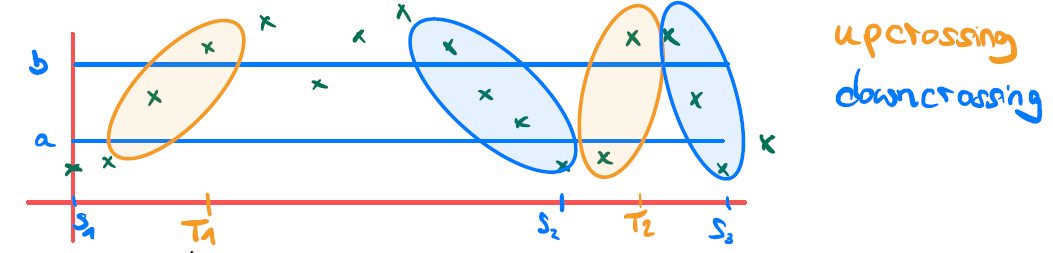
\includegraphics[scale=0.5]{plot321}
%\end{figure}
More formally, we define the crossing times by
\begin{align*}
	S_1 &\coloneqq 0 \\
		T_1 &\coloneqq \min\lbrace n\in \mathbb{N}_0: X_n \geq b \rbrace \\
	S_{k+1} &\coloneqq \min\lbrace n > T_k: X_n \leq a \rbrace \\
	T_{k+1} &\coloneqq \min\lbrace n > S_k: X_n \geq b \rbrace
\end{align*}
and set $$U_n[a,b]\coloneqq \sum\limits_{k=1}^{\infty}\mathbf 1_{T_k \leq n},$$ which is the number of finished upcrosings up to time $n$. The main ingredient towards the convergence theorem is the following estimate for the number of upcrossings:
\begin{llemma}
\begin{lemma}[Doob's upcrossing inequality]\label{upcrossing_inequality}
	If $(X_n)_{n\in\mathbb{N}_0}$ is a (sub)martingale and $a<b$, then $$ \E\big[ U_n[a,b]\big] \leq \frac{\E\big[ (X_n-a)^+ - (X_0-a)^+ \big]}{b-a}.$$
\end{lemma}
\end{llemma}
\begin{proof}[Proof]
	%		\begin{figure}[H]
	%			\includegraphics[scale=0.4]{mart2.jpeg}
	%			\vspace{-5mm}
	%			\caption*{Realisation of $X$ with four upcrossings and the counting using $H$, $Y$, and $H\cdot Y$}
	%		\end{figure}	
	In order to count the number of upcrossings we introduce 	 
	\begin{align*}
		Y_n&:= \max\{X_n,a\}=(X_n-a)^++a,\\
		H_n &\coloneqq \sum\limits_{k=1}^{\infty}\mathbf 1_{\{S_k<n\leq T_k\}}=\begin{cases}1&: n\in \{S_k+1,...,T_k\}\text{ for some }k\\0&:n\in \{T_k+1,...,S_k\}\text{ for some }k \end{cases}.
	\end{align*}	
	Additionally, we are interested in the discrete stochastic integral $H\cdot Y$. The idea of the proof is best understood through the illustration of the processes. 
	
	\begin{figure}
		\vspace{2mm}
		\begin{center}
		  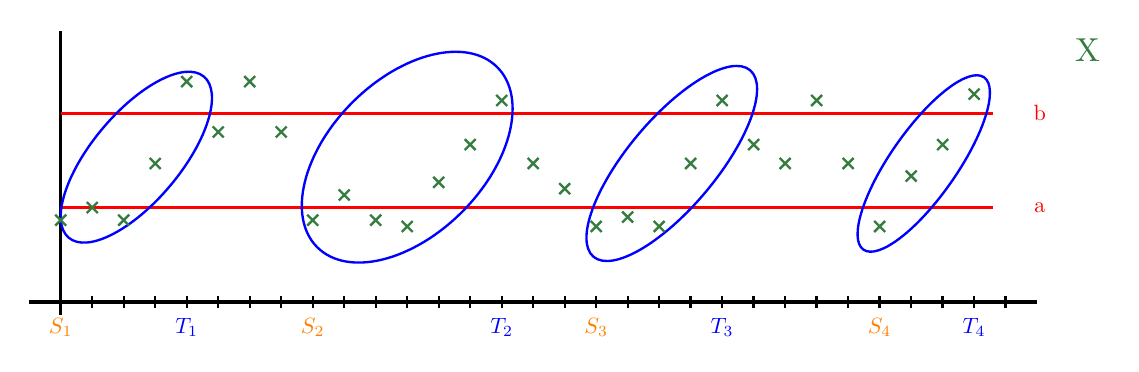
\begin{tikzpicture}[scale=0.8,transform shape]
		  \tikzset{
			cross/.pic ={
			  \draw[pic actions,rotate=#1,line width=0.3mm] 
				(-3.5pt,0) -- (3.5pt,0)
				(0,-3.5pt) -- (0,3.5pt);
			},
		  }
		  \tikzset{
			pics/tick/.style args={#1}{code={
			  \draw[line width=0.3mm] (0,-#1) -- (0,#1) ;
			  },
			}
		  }
		  %LABEL
		  \node[darkgreen,scale=1.5] (X) at (16.3,4) {X};
		  %AXIS Y
		  \draw[black,line width=0.4mm] (0,-0.2) -- ++(90:4.5cm);
		  %AXIS X 
		  \draw[black,line width=0.4mm] (-0.5,0) --++(0:16cm); 
		  %AXIS TICKS 
		  \foreach \x in {0,0.5,...,15}{
			\draw (\x,0) pic {tick={1mm}}  ;
		  }
		  %a ,b intervall
		  \draw[red,line width=0.4mm] (0,3) -- (14.8,3) node[red,pos=1.05] (b) {b};
		  \draw[red,line width=0.4mm] (0,1.5) -- (14.8,1.5) node[red,pos=1.05] (a) {a};
		
		  %LABELS  S 
		  \foreach \x [count=\i] in {0,4,8.5,13}{
		  \node[orange,yshift=-4mm] (S\i) at (\x,0) {$S_{\i}$} ;
		  }
		  %LABEL T
		  \foreach \x [count=\i] in {2,7,10.5,14.5}{
		  \node[blue,yshift=-4mm] (T\i) at (\x,0) {$T_{\i}$} ;
		  }
		  
		  %ELLIPSE 1 
		  \node[ellipse,draw=blue,minimum height=40pt,minimum width=95pt,rotate=50,line width=0.3mm] (e1) at (1.2,2.3) {};
		  %ELLIPSE 2 
		  \node[ellipse,draw=blue,minimum height=70pt,minimum width=115pt,rotate=45,line width=0.3mm] (e2) at (5.5,2.3) {};
		  %ELLIPSE 3 
		  \node[ellipse,draw=blue,minimum height=40pt,minimum width=110pt,rotate=50,line width=0.3mm] (e3) at (9.7,2.2) {};
		  %ELLIPSE 4 
		  \node[ellipse,draw=blue,minimum height=30pt,minimum width=95pt,rotate=55,line width=0.3mm] (e4) at (13.7,2.2) {};
		
		  %CROSS ELLIPSE 1 
		  \begin{scope}
		  \draw[darkgreen] (0,1.3) pic {cross={45}} ;
		  \draw[darkgreen] (0.5,1.5) pic {cross={45}} ;
		  \draw[darkgreen] (1,1.3) pic {cross={45}} ;
		  \draw[darkgreen] (1.5,2.2) pic {cross={45}} ;
		  \draw[darkgreen] (2,3.5) pic {cross={45}} ;  
		  \end{scope}
		  %CROSS GAP 1 
		  \begin{scope}
		  \draw[darkgreen] (2.5,2.7) pic {cross={45}} ;
		  \draw[darkgreen] (3,3.5) pic {cross={45}} ;
		  \draw[darkgreen] (3.5,2.7) pic {cross={45}} ; 
		  \end{scope}
		  %CROSS ELLIPSE 2 
		  \begin{scope}[xshift=0]
		  \draw[darkgreen] (4,1.3) pic {cross={45}} ;
		  \draw[darkgreen] (4.5,1.7) pic {cross={45}} ;
		  \draw[darkgreen] (5,1.3) pic {cross={45}} ;
		  \draw[darkgreen] (5.5,1.2) pic {cross={45}} ;
		  \draw[darkgreen] (6,1.9) pic {cross={45}} ;
		  \draw[darkgreen] (6.5,2.5) pic {cross={45}} ;
		  \draw[darkgreen] (7,3.2) pic {cross={45}} ;
		  \end{scope}
		  %CROSS GAP 2
		  \begin{scope}
		  \draw[darkgreen] (7.5,2.2) pic {cross={45}} ;  
		  \draw[darkgreen] (8,1.8) pic {cross={45}} ;  
		  \end{scope}
		  %CROSS ELLIPSE 3
		  \begin{scope}  
		  \draw[darkgreen] (8.5,1.2) pic {cross={45}} ;  
		  \draw[darkgreen] (9,1.35) pic {cross={45}} ;  
		  \draw[darkgreen] (9.5,1.2) pic {cross={45}} ; 
		  \draw[darkgreen] (10,2.2) pic {cross={45}} ; 
		  \draw[darkgreen] (10.5,3.2) pic {cross={45}} ; 
		  \end{scope}
		  %CROSS GAP 3 
		  \begin{scope}
		  \draw[darkgreen] (11,2.5) pic {cross={45}} ;  
		  \draw[darkgreen] (11.5,2.2) pic {cross={45}} ;  
		  \draw[darkgreen] (12,3.2) pic {cross={45}} ; 
		  \draw[darkgreen] (12.5,2.2) pic {cross={45}} ; 
		  \end{scope}
		  %CROSS ELLIPSE 4 
		  \begin{scope}
		  \draw[darkgreen] (13,1.2) pic {cross={45}} ; 
		  \draw[darkgreen] (13.5,2) pic {cross={45}} ; 
		  \draw[darkgreen] (14,2.5) pic {cross={45}} ; 
		  \draw[darkgreen] (14.5,3.3) pic {cross={45}} ; 
		  \end{scope}
		  \end{tikzpicture}   
		\vspace*{1cm}
		  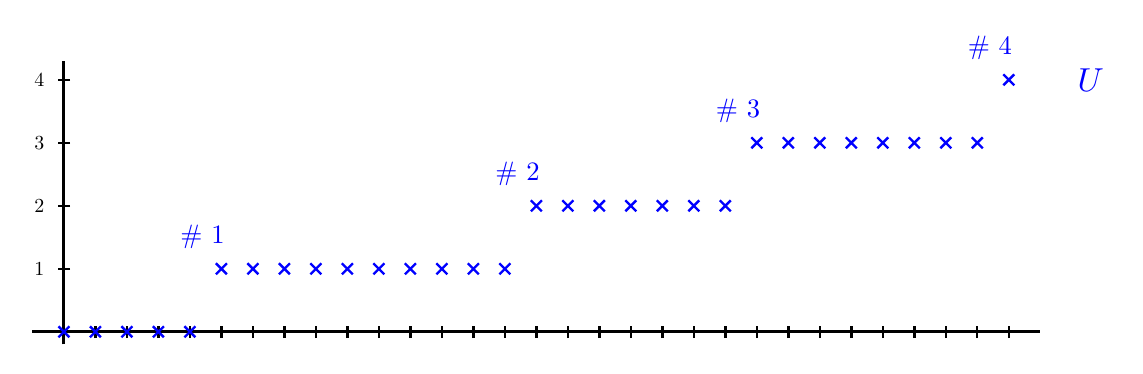
\begin{tikzpicture}[scale=0.8,transform shape]
		
		  \tikzset{
			cross/.pic ={
			  \draw[pic actions,rotate=#1,line width=0.3mm]
				(-3.5pt,0) -- (3.5pt,0)
				(0,-3.5pt) -- (0,3.5pt);
			},
		  }
		  \tikzset{
			pics/tick/.style args={#1}{code={
			  \draw[line width=0.3mm] (0,-#1) -- (0,#1) ;
			  },
			}
		  }
		  %LABEL
		  \node[blue,scale=1.5] (U) at (16.3,4) {$U$};
		  %AXIS Y
		  \draw[black,line width=0.4mm] (0,-0.2) -- ++(90:4.5cm);
		  %AXIS X
		  \draw[black,line width=0.4mm] (-0.5,0) --++(0:16cm);
		  %AXIS TICKS
		  \foreach \x in {0,0.5,...,15}{
			\draw (\x,0) pic {tick={1mm}}  ;
		  }
		  \foreach \y in {1,...,4}{
			\draw (0,\y) pic[rotate=90] {tick={1mm}} node[left,xshift=-2mm,scale=0.9] {\y} ;
		  }
		  \node[blue,scale=1.2] at (2.2,1.5) {\# 1};
		  \foreach \x in {0,0.5,...,2}{
			\draw (\x,0) pic[blue] {cross={45}}; 
		  }
		  \node[blue,scale=1.2] at (7.2,2.5) {\# 2};
		  \foreach \x in {2.5,3,...,7}{
			\draw (\x,1) pic[blue] {cross={45}}; 
		  }
		  \node[blue,scale=1.2] at (10.7,3.5) {\# 3};
		  \foreach \x in {7.5,8,...,10.5}{
			\draw (\x,2) pic[blue] {cross={45}}; 
		  }
		  \node[blue,scale=1.2] at (14.7,4.5) {\# 4};
		  \foreach \x in {11,11.5,...,14.5}{
			\draw (\x,3) pic[blue] {cross={45}}; 
		  }
		  \draw (15,4) pic[blue] {cross={45}};
		  \end{tikzpicture}
						  \vspace*{0cm}
		 \hspace*{0.35cm}
		  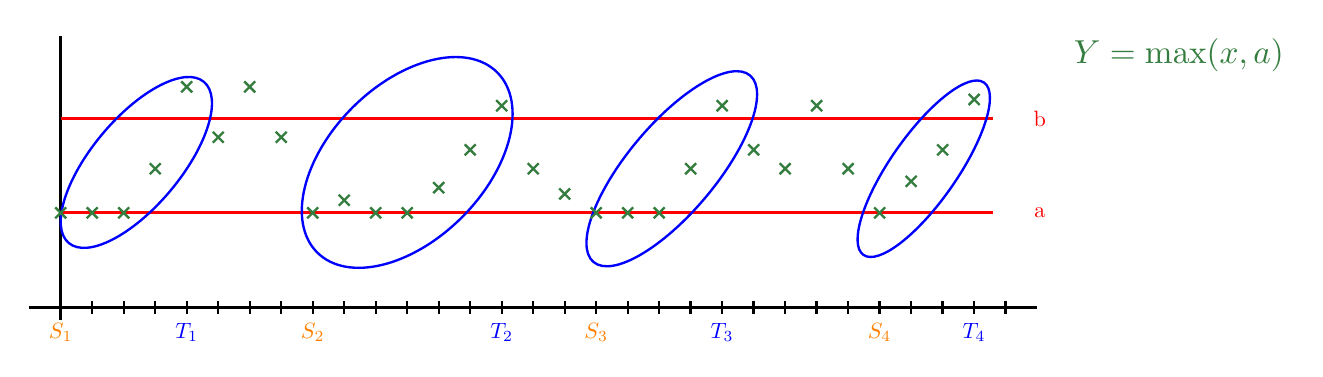
\begin{tikzpicture}[scale=0.8,transform shape]
		  \tikzset{
			cross/.pic ={
			  \draw[pic actions,rotate=#1,line width=0.3mm] 
				(-3.5pt,0) -- (3.5pt,0)
				(0,-3.5pt) -- (0,3.5pt);
			},
		  }
		  \tikzset{
			pics/tick/.style args={#1}{code={
			  \draw[line width=0.3mm] (0,-#1) -- (0,#1) ;
			  },
			}
		  }
		  %LABEL
		  \node[darkgreen,scale=1.5,xshift=5mm] (Y) at (17,4) {$Y=\max(x,a)$};
		  %AXIS Y
		  \draw[black,line width=0.4mm] (0,-0.2) -- ++(90:4.5cm);
		  %AXIS X 
		  \draw[black,line width=0.4mm] (-0.5,0) --++(0:16cm); 
		  %AXIS TICKS 
		  \foreach \x in {0,0.5,...,15}{
			\draw (\x,0) pic {tick={1mm}}  ;
		  }
		  %a ,b intervall
		  \draw[red,line width=0.4mm] (0,3) -- (14.8,3) node[red,pos=1.05] (b) {b};
		  \draw[red,line width=0.4mm] (0,1.5) -- (14.8,1.5) node[red,pos=1.05] (a) {a};
		
		  %LABELS  S 
		  \foreach \x [count=\i] in {0,4,8.5,13}{
		  \node[orange,yshift=-4mm] ($S_{\i}$) at (\x,0) {$S_{\i}$} ;
		  }
		  %LABEL T
		  \foreach \x [count=\i] in {2,7,10.5,14.5}{
		  \node[blue,yshift=-4mm] ($T_{\i}$) at (\x,0) {$T_{\i}$} ;
		  }
		  
		  %ELLIPSE 1 
		  \node[ellipse,draw=blue,minimum height=40pt,minimum width=95pt,rotate=50,line width=0.3mm] (e1) at (1.2,2.3) {};
		  %ELLIPSE 2 
		  \node[ellipse,draw=blue,minimum height=70pt,minimum width=115pt,rotate=45,line width=0.3mm] (e2) at (5.5,2.3) {};
		  %ELLIPSE 3 
		  \node[ellipse,draw=blue,minimum height=40pt,minimum width=110pt,rotate=50,line width=0.3mm] (e3) at (9.7,2.2) {};
		  %ELLIPSE 4 
		  \node[ellipse,draw=blue,minimum height=30pt,minimum width=95pt,rotate=55,line width=0.3mm] (e4) at (13.7,2.2) {};
		
		  %CROSS ELLIPSE 1 
		  \begin{scope}
		  \draw[darkgreen] (0,1.5) pic {cross={45}} ;
		  \draw[darkgreen] (0.5,1.5) pic {cross={45}} ;
		  \draw[darkgreen] (1,1.5) pic {cross={45}} ;
		  \draw[darkgreen] (1.5,2.2) pic {cross={45}} ;
		  \draw[darkgreen] (2,3.5) pic {cross={45}} ;  
		  \end{scope}
		  %CROSS GAP 1 
		  \begin{scope}
		  \draw[darkgreen] (2.5,2.7) pic {cross={45}} ;
		  \draw[darkgreen] (3,3.5) pic {cross={45}} ;
		  \draw[darkgreen] (3.5,2.7) pic {cross={45}} ; 
		  \end{scope}
		  %CROSS ELLIPSE 2 
		  \begin{scope}[xshift=0]
		  \draw[darkgreen] (4,1.5) pic {cross={45}} ;
		  \draw[darkgreen] (4.5,1.7) pic {cross={45}} ;
		  \draw[darkgreen] (5,1.5) pic {cross={45}} ;
		  \draw[darkgreen] (5.5,1.5) pic {cross={45}} ;
		  \draw[darkgreen] (6,1.9) pic {cross={45}} ;
		  \draw[darkgreen] (6.5,2.5) pic {cross={45}} ;
		  \draw[darkgreen] (7,3.2) pic {cross={45}} ;
		  \end{scope}
		  %CROSS GAP 2
		  \begin{scope}
		  \draw[darkgreen] (7.5,2.2) pic {cross={45}} ;  
		  \draw[darkgreen] (8,1.8) pic {cross={45}} ;  
		  \end{scope}
		  %CROSS ELLIPSE 3
		  \begin{scope}  
		  \draw[darkgreen] (8.5,1.5) pic {cross={45}} ;  
		  \draw[darkgreen] (9,1.5) pic {cross={45}} ;  
		  \draw[darkgreen] (9.5,1.5) pic {cross={45}} ; 
		  \draw[darkgreen] (10,2.2) pic {cross={45}} ; 
		  \draw[darkgreen] (10.5,3.2) pic {cross={45}} ; 
		  \end{scope}
		  %CROSS GAP 3 
		  \begin{scope}
		  \draw[darkgreen] (11,2.5) pic {cross={45}} ;  
		  \draw[darkgreen] (11.5,2.2) pic {cross={45}} ;  
		  \draw[darkgreen] (12,3.2) pic {cross={45}} ; 
		  \draw[darkgreen] (12.5,2.2) pic {cross={45}} ; 
		  \end{scope}
		  %CROSS ELLIPSE 4 
		  \begin{scope}
		  \draw[darkgreen] (13,1.5) pic {cross={45}} ; 
		  \draw[darkgreen] (13.5,2) pic {cross={45}} ; 
		  \draw[darkgreen] (14,2.5) pic {cross={45}} ; 
		  \draw[darkgreen] (14.5,3.3) pic {cross={45}} ; 
		  \end{scope}
		  \end{tikzpicture} 
		  \vspace*{0.5cm}
		  \hspace*{-0.4cm}
		  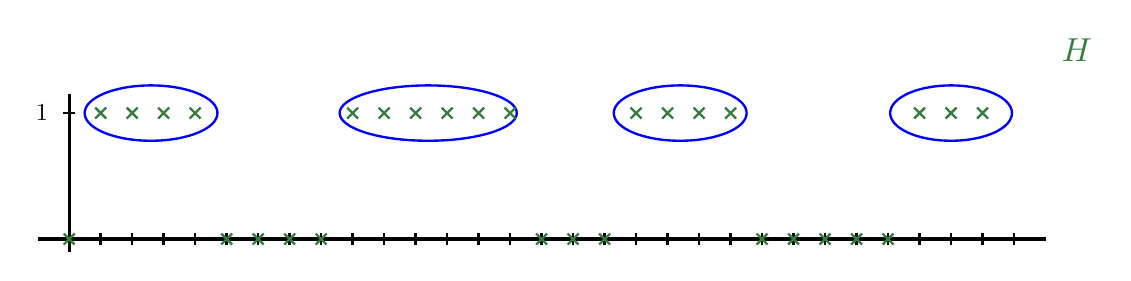
\begin{tikzpicture}[scale=0.8,transform shape]
		  \tikzset{
			cross/.pic ={
			  \draw[pic actions,rotate=#1,line width=0.3mm]
				(-3.5pt,0) -- (3.5pt,0)
				(0,-3.5pt) -- (0,3.5pt);
			},
		  }
		  \tikzset{
			pics/tick/.style args={#1}{code={
			  \draw[line width=0.3mm] (0,-#1) -- (0,#1) ;
			  },
			}
		  }
		  %LABEL
		  \node[darkgreen,scale=1.5] (H) at (16,3) {$H$};
		  %AXIS Y
		  \draw[black,line width=0.4mm] (0,-0.2) -- ++(90:2.5cm);
		  %AXIS X
		  \draw[black,line width=0.4mm] (-0.5,0) --++(0:16cm);
		  %AXIS TICKS
		  \foreach \x in {0,0.5,...,15}{
			\draw (\x,0) pic {tick={1mm}}  ;
		  }
		  \draw (0,2) pic[rotate=90] {tick={1mm}} node[left,xshift=-2mm,scale=1.1] {1} ;
		  
		  \draw(0,0) pic[darkgreen] {cross={45}};
		  %ELLIPSE 1
		  \node[ellipse,draw=blue,minimum height=25pt,minimum width=60pt,rotate=0,line width=0.3mm] (e2) at (1.3,2) {};
		  \foreach \x in {0.5,1,...,2}{
			\draw (\x,2) pic[darkgreen] {cross={45}}; 
		  }
		  %
		  \foreach \x in {2.5,3,3.5,4}{
			\draw (\x,0) pic[darkgreen] {cross={45}};
		  }
		  %ELLIPSE 2
		  \node[ellipse,draw=blue,minimum height=25pt,minimum width=80pt,rotate=0,line width=0.3mm] (e2) at (5.7,2) {};
		  \foreach \x in {4.5,5,...,7}{
			\draw (\x,2) pic[darkgreen] {cross={45}}; 
		  }
		  %
		  \foreach \x in {7.5,8,8.5}{
			\draw (\x,0) pic[darkgreen] {cross={45}}; 
		  }
		  %ELLIPSE 3
		  \node[ellipse,draw=blue,minimum height=25pt,minimum width=60pt,rotate=0,line width=0.3mm] (e3) at (9.7,2) {};
		  \foreach \x in {9,9.5,10,10.5}{
			\draw (\x,2) pic[darkgreen] {cross={45}}; 
		  }
		  %
		  \foreach \x in {11,11.5,...,13}{
			\draw (\x,0) pic[darkgreen] {cross={45}};
		  }
		
		  %ELLIPSE 4
		  \node[ellipse,draw=blue,minimum height=25pt,minimum width=55pt,rotate=0,line width=0.3mm] (e4) at (14,2) {};
		  \foreach \x in {13.5,14,14.5}{
			\draw (\x,2) pic[darkgreen] {cross={45}};
		  }
		  \end{tikzpicture}
		  \hspace*{-0.5cm}
		  \begin{tikzpicture}[scale=0.8,transform shape]
		  \tikzset{
			cross/.pic ={
			  \draw[pic actions,rotate=#1,line width=0.3mm]
				(-3.5pt,0) -- (3.5pt,0)
				(0,-3.5pt) -- (0,3.5pt);
			},
		  }
		  \tikzset{
			pics/tick/.style args={#1}{code={
			  \draw[line width=0.3mm] (0,-#1) -- (0,#1) ;
			  },
			}
		  }
		  %LABEL
		  \node[darkgreen,scale=1.5] (HY) at (16.5,3) {$H\cdot Y$};
		  %AXIS Y
		  \draw[black,line width=0.4mm] (0,-0.2) -- ++(90:6.5cm);
		  %AXIS X
		  \draw[black,line width=0.4mm] (-0.5,0) --++(0:16cm);
		  %AXIS TICKS
		  \foreach \x in {0,0.5,...,15}{
			\draw (\x,0) pic {tick={1mm}}  ;
		  }
		
		  %LABELS  S 
		  \foreach \x [count=\i] in {0,4,8.5,13}{
		  \node[orange,yshift=-4mm] ($S_{\i}$) at (\x,0) {$S_{\i}$} ;
		  }
		  %LABEL T
		  \foreach \x [count=\i] in {2,7,10.5,14.5}{
		  \node[blue,yshift=-4mm] ($T_{\i}$) at (\x,0) {$T_{\i}$} ;
		  }
		  %BRACKETS 
		  %b-a = 1.5
		  \foreach \i [count=\j] in {0.1,1.6,3.1,4.6}{ 
			\pgfmathsetmacro\res{\i+1.4}
			\draw[decorate,decoration={brace,raise=0mm},draw=blue,line width=0.4mm,xshift=-2mm,scale=0.98] (0,\i) -- (0,\res) node[blue,anchor=north,yshift=-0mm,pos=0.73,xshift=-8mm,scale=0.9] (B\j) {$\ge b-a$}; 
		  }
		  \foreach \x in {1,2,3,4}{
			\draw[blue,line width =0.4mm] ($(S\x) - (0,4mm)$) -- ($(T\x)-(0,4mm)$);
		  }  
		  \foreach \x in {0,0.5,1}{
			\draw (\x,0) pic[darkgreen] {cross={45}};
		  }
		  \draw (1.5,0.7) pic[darkgreen] {cross={45}};
		
		  \foreach \x in {2,2.5,...,4}{
			\draw (\x,1.4) pic[darkgreen] {cross={45}};
		  }
		
		  \foreach \x in {4.5,5,5.5}{
			\draw (\x,1.7) pic[darkgreen] {cross={45}};
		  }
			\draw (6,1.9) pic[darkgreen] {cross={45}};
			\draw (6.5,2.4) pic[darkgreen] {cross={45}};
		
		  \foreach \x in {7,7.5,...,9.5}{
			\draw (\x,3) pic[darkgreen] {cross={45}};
		  }
		  \draw (10,3.8) pic[darkgreen] {cross={45}};
		  \foreach \x in {10.5,11,...,13}{
			\draw (\x,4.4) pic[darkgreen] {cross={45}};
		  }
		  \draw (13.5,5) pic[darkgreen] {cross={45}};
		  \draw (14,5.5) pic[darkgreen] {cross={45}};
		  \draw (14.5,6) pic[darkgreen] {cross={45}};
		
		  % \draw[dashed,blue,line width=0.4mm] ($(B4) + (10mm,0.6)$) -- (14.5,6);
		  \draw[dashed,blue,line width=0.2mm] (0,1.4) -- (1.8,1.4);
		  \draw[dashed,blue,line width=0.2mm] (0,3) -- (6.8,3);
		  \draw[dashed,blue,line width=0.2mm] (0,4.4) -- (10.3,4.4);
		  \draw[dashed,blue,line width=0.2mm] (0,6) -- (14.5,6);

		  \end{tikzpicture}
		  \vspace{3mm}
				  \caption*{Realisation of $X$ with four upcrossings and the counting using $Y$, $H$, and $H\cdot Y$}

		\end{center}
		\end{figure}
	We have chosen $H$ such that $H$ only takes the values $1$ and $0$ so that $H\cdot Y$ either stays constant (in intervals with $H=0$) or sums up the increments of $Y$. Every upcrossing of $X$ yields an increase of $H\cdot Y$ of at least $b-a$ so that $H\cdot Y$ counts (up to a factor $b-a$) the number of upcrossings.\smallskip
	
	Let's have a more formal look a the definitions. The telescopic sum property is best seen at the endpoints of upcrossings by removing all $0$ summmands:
			\begin{align*}
				(H\cdot Y)_{T_n} &=  \sum_{k=1}^{T_n}H_k(Y_k-Y_{k-1}) \\
							&= \sum_{k=1}^{n}\sum_{j=S_k+1}^{T_k}1\cdot (Y_j-Y_{j-1}) \\
							\overset{\text{telescope}}&{=} \sum_{k=1}^{n}(Y_{T_k}-Y_{S_k})	\\
							&\geq n\cdot (b-a)
			\end{align*}
			because $Y_{T_k}\geq b$ and $Y_{S_k} \leq a$. Now let us have a look at the values of $H\cdot Y$ in the two different ranges of the definition of $H$:			
		\begin{align*}
			(H\cdot Y)_j \overset{\text{adding }0s}{=} (H\cdot Y)_{T_n}\geq n(b-a),\quad \forall  j\in\lbrace T_n, \cdots,S_{n+1}\rbrace
		\end{align*}
		and, using this equality again,
		\begin{align*}
			(H\cdot Y)_j \overset{\text{telescope}}{\geq} (H\cdot Y)_{S_{n+1}} \overset{\text{adding }0s}{=} (H \cdot Y)_{T_n}\geq n(b-a),\quad\forall j\in \lbrace S_{n+1},\cdots,T_{n+1}-1 \rbrace.
		\end{align*}
	Noting that $j\geq T_n$ is the same as $n\geq U_j[a,b]$ (recall the definitions of $T_n$ and $U_j[a,b]$) we obtain
	\begin{align*}
		(H\cdot Y)_n \geq (b-a)U_n[a,b],\quad n\in\N_0.
	\end{align*}
	We are now close to finishing the proof using a submartingale argument. First note that $Y$ is a submartingale by Proposition \ref{prop314} as $x\mapsto (x-a)^++a$ is a convex function. Next, $H_n$ is previsible as $\mathbf 1_{\{S_k<n\leq T_k\}} = \mathbf 1_{\{S_k<n\}}\cdot \mathbf 1_{\{T_k<n\}^C}$ and sums and limits of measurable functions are measurable (compare \ref{hilf} and \ref{mlimits}). Hence, also $1-H_n$ is previsible so that  the discrete integral $(1-H)\cdot X$ is a submartingale by Theorem \ref{you_cannot_beat_the_system} because $1-H_n$ is bounded by $1$ and non-negative. But then, using that submartingales have increasing expectation, we obtain the desired bound:
	\begin{align*}
		\E[Y_n - Y_0] \overset{\text{telescope}}&{=} \E[(1\cdot Y)_n]\\
		 &= \E[(H\cdot Y)_n] + \E[((1-H)\cdot Y)_n]\\ 
		 \overset{\text{see above}}&{\geq} (b-a) \E\big[ U_n[a,b]\big] +  \E[((1-H)\cdot Y)_n] \\
		 \overset{(1-H)\cdot Y \text{ submart.}}&{\geq} (b-a) \E\big[ U_n[a,b]\big] + \E\big[ ( (1-H)\cdot Y )_0\big] \\
		&= (b-a) \E\big[ U_n[a,b]\big] + 0.
	\end{align*}
	Dividing by $b-a$ and plugging-in the definition of $Y$ yields the upcrossing inequality.
\end{proof}
With the upcrossing lemma we can quickly finish the proof of the martingale convergence theorem. The proof looks much worse than it is!
\begin{proof}[Proof of the almost sure martingale convergence theorem]
	Let $a<b$. Since $(X_n-a)^+ \leq \lvert a \rvert + X_n^+$ the upcrossing inequality gives $$ \E\big[ U_n[a,b]\big] \leq \frac{a+\E[X_n^+]}{b-a}$$
	and the right hand side is bounded by some $C<\infty$ due to the assumption on the submartingale. Now define
	\begin{align*}
		U[a,b]:=\lim_{n\to\infty} U_n[a,b]\in [0,\infty],
	\end{align*}	
	which is the total number of upcrossings through $[a,b]$. The limit exists as monotone sequences converge (with possible limit $+\infty$). Since the limit is monotone in $n$ we can use the monotone convergence theorem to obtain
	\begin{align*}
		\E\big[ U_n[a,b]\big] = \lim_{n\to \infty}\E\big[U_n[a,b]\big] \leq C.
	\end{align*}
	Since non-negative random variables with finite expectation are finite almost surely, we proved that $$\mathbb{P}(U[a,b]< \infty )=1,\quad \text{ for all }a<b.$$ Hence, we proved that almost surely the submartingale only crosses $[a,b]$ finitely often. If we define
	\begin{align*}
		C^{a,b} := \lbrace \omega: U[a,b](\omega) = \infty \rbrace \quad \text{and}\quad
		C := \bigcup_{a,b\in\mathbb{Q},\: a<b}C^{a,b},
	\end{align*}
	then the above shows that $\mathbb{P}(C^{a,b}) = 0$ and, hence, $\mathbb{P}(C)=0$. Since $C^C$ is the event that $X$ does not cross any interval infinitely often (equivalently, $X_n$ converges) and $\P(C^C)=1$ we proved that $\lim_{n\to\infty} X_n$ exists almost surely (with a possibly infinite limit).\smallskip
	
	Now define $X_\infty:=\lim_{n\to\infty} X_n$. Since all $X_n$ are $\cF_{\infty}$-measurable, $X_{\infty}$ is $\cF_{\infty}$-measurable as a limit. If we can show that $\E[|X_\infty|]<\infty$, then $X_\infty$ is finite almost surely. To show this we use Fatou's lemma twice. First, 
	\begin{align*}
		\E[X_{\infty}^-] \leq \liminf_{n\to\infty} \E[X_n^-] 
								= \liminf_{n\to\infty} \big( \E[X_n^+]-\E[X_n]\big) 
								\leq \sup_{n\in\N_0} \E[X_n^+] - \E[X_0] < \infty
	\end{align*}
	and, secondly,
	\begin{align*}
		\E[X_{\infty}^+] \leq \liminf_{n\to\infty} \E[X_n^+] <\infty.
	\end{align*}
	Hence, $\E[\lvert X_{\infty}\rvert ] < \infty$ and in particular $\lvert X_{\infty} \rvert < \infty$ a.s.
\end{proof}
A typical example for the martingale convergence theorem is a better understanding of the regimes in the branching process from Example \ref{GW}.
\begin{example}\label{branching1}
Recall the martingale $M$ obtained from the branching process which is actually a non-negative martingale. Hence, by Corollary \ref{MMM} there is a finite almost sure limit $M_{\infty}$ of $M_n$ which directly translates into knowledge on $X$. Here is an important fact that we use: If a sequence with values on $\N_0$ converges, then the sequence must ultimately be constant.
			\begin{enumerate}[label=(\roman*)]	
				\item 
				$\mu < 1$ (subcritical case): \\
					$\frac{1}{\mu^n} \to \infty$, so that $X_n = \mu^n M_n \to 0$, $n \to \infty$. But then the population modelled by $X$ suffers extinction in finite time almost surely, that is, almost surely gets absorbed at $0$ after some (unknown) random time $N(\omega)$.
				\item
					$\mu = 1$ (critical case): \\
					$(X_n)_{n\in\mathbb{N}}$ itself is a non-negative martingale so that $X_n \to X_{\infty}$ a.s. But how could the branching process stop moving ultimately? Right, only by almost sure extinct of the population in finite time (check the definition).
				\item
					$\mu > 1$ (supercritical case): \\
					Again the martingale convergence theorem implies
					$$\frac{1}{\mu^n}\cdot X_n \to M_{\infty}\in [0,\infty).$$
					Unfortunately, so far do not know anything about $M_\infty$ except being finite. On the event $E:=\lbrace\omega: M_{\infty}(\omega)> 0 \rbrace$ we observe exponential growth of the population, namely, $$X_n(\omega) \sim M_\infty(\omega) \mu^n = M_\infty (\omega) e^{\log(\mu)\cdot n}.$$ So far we cannot say if $E$ has positive probability. Under a square-integrability condition we will solve this question using the $L^2$-martingale convergence theorem below.
			\end{enumerate}
			What we see is an effect everyone learnt during the Covid pandemic. Sick people infecting on average more than $1$ person can lead to exponential growth, infecting on average less than $1$ person leads to extinction of the disease. Of course, this model is very simplistic due to the iid assumption on the offspring.
			
\end{example}
	\marginpar{\textcolor{red}{Lecture 7}}

\subsection{$L^p$-martingale convergence theorem for $p>1$}
After the almost sure convergence we now look for stronger conditions on martingales that additionally ensure convergence of $X_n$ towards $X_\infty$ in $L^p$, i.e. $\lim_{n\to\infty}\E[|X_n-X_\infty|^p]=0$. If you forgot about the $L^p$-spaces of random variables (modulo zero sets) with the norms $||X||_p=\E[|X|^p]^{1/p}$ please check Theorem \ref{Lp} and the discussion around. In this and the following section bounded sets in $L^p$ and $L^1$ will play a crucial role. Recall from analysis that bounded subsets of a normed space are subsets that lie in a ball with respect to the norm. In a sketchy picture (ignoring the linear structure) the situation looks as follows. 
\begin{figure}[h]
\begin{center}
  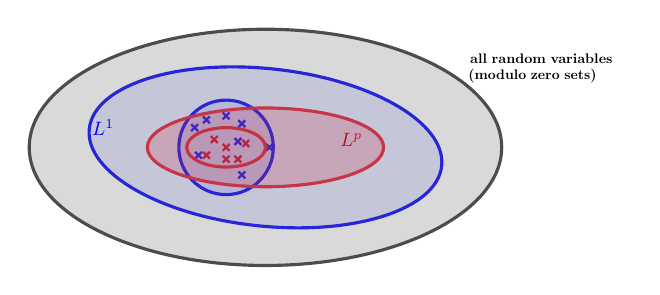
\begin{tikzpicture}[scale=0.5,transform shape]
  \tikzset{
    cross/.pic ={
      \draw[pic actions,rotate=#1,line width=0.3mm]
        (-3.5pt,0) -- (3.5pt,0)
        (0,-3.5pt) -- (0,3.5pt);
    },
  }
  \definecolor{darkred}{RGB}{168,27,27};
  \foreach \x/\y in {-1/0.8, -1.5/0.7, -1.8/0.5 , -0.6/0.6 , 0.1/0, -0.6/-0.7 , -1.7/-0.2,-0.7/0.15} {
    \draw (\x,\y) pic[blue] {cross={45}};
  } 
  \foreach \x/\y in {-1/0, -1.3/0.2,-1.5/-0.2,-1/-0.3,-0.7/-0.3,-0.5/0.1}{
    \draw (\x,\y) pic[red] {cross={45}};
  } 
  \draw[draw=blue!100,line width=0.4mm,fill=blue,fill opacity=0.1,rotate=0] (-1,0) ellipse (1.2 and 1.2);
  \draw[draw=red!90,line width=0.4mm,fill=red,fill opacity=0,rotate=0] (-1,0) ellipse (1 and 0.5);
  \draw[draw=red!90,line width=0.4mm,fill=red,fill opacity=0.2,rotate=0] (0,0) ellipse (3 and 1);
  \draw[draw=blue!100,line width=0.4mm,fill=blue,fill opacity=0.1,rotate=-6] (0,0) ellipse (4.5 and 2);
  \draw[draw=black!70,line width=0.4mm,fill=gray,fill opacity=0.3] (0,0) ellipse (6 and 3) ;
  \node[black,text width=4cm] at (7.2,2) {\textbf{all random variables (modulo zero sets)}};
  \node[blue,text width=2cm,scale=1.4] at (-3,0.5) {$L^1$};
  \node[darkred,text width=2cm,scale=1.4] at (3.3,0.2) {$L^p$};
  \end{tikzpicture} 
  \caption*{A schematic drawing of bounded sets of random variables in $L^p$ and $L^1$}
  \end{center}
\end{figure}
In this section we will show that martingales that are bounded in $L^p$ automatically converge in $L^p$ to a limit $X_\infty$. This feature of martingales is very special as typically one should not hope for convergence of a sequence only from knowing it is bounded. Martingales are just amazing!\smallskip




%Recall that convergence in $L^p$ means $\lim_{n\to\infty}\E[|X_n-X_\infty|^p]=0$. But since convergence in normed spaces implies convergence of the norms (norms are continuous) we would obtain $\lim_{n\to\infty}\E[|X_n|^p]=\E[|X_\infty|^p]$. So the very least one should assume to hold is boundedness of the $p$th moments as otherwise convergence is impossible. One of the magic features of martingales is that this condition is also enough. \smallskip

The estimates we develop are almost more important than the theorem itself, most importantly, Doob's inequalities for the so-called running supremum $X^*:=\max_{k\leq n} X_k$ appears in many places of probability theory. We start with a continuation of the optional sampling theorem:
\begin{llemma}
\begin{lemma}\label{lemma331}
	Let $(X_n)_{n\in\mathbb{N}_0}$ be an $(\cF_n)$-(sup)martingale and $S$, $T$ bounded $(\cF_n)$-stopping times with $S \leq T$ almost surely. Then
	\begin{enumerate}[label=(\roman*)]	
		\item
			$\E[X_S] \leq \E[X_T]$
		\item
			$\E[X_T\,|\,\cF_s] \geq X_s$, i.e. the (sup)martingale property also holds at bounded stopping times.
	\end{enumerate}
\end{lemma}
\end{llemma}
\begin{proof}
	\begin{enumerate}[label=(\roman*)]	
		\item The first claim is left as an exercise:
		\begin{luebung}
		Do you remember the proof of the optional sampling theorem sketched below Theorem \ref{you_cannot_beat_the_system}? The same trick can be used here using $H_n = \mathbf 1_{S < n \leq T}$. Do it!
		\end{luebung}
		\item First recall a general fact: If $X$ is a random variable on $(\Omega,\cA,\mathbb{P})$ with $\int_A X \dint \mathbb{P} \geq 0$ for all $A \in \cA$, then $X \geq 0 $ a.s. This follows directly by using the sets $A=\{X\leq 0\}$ and Theorem \ref{S7} (iii).\smallskip
		
		To use this fact we show $*$ in		
			\begin{align*}
				\E\big[ \E[ X_T\,|\,\cF_S]\mathbf 1_A \big] \overset{\text{cond. exp.}}{=} \E[X_T \mathbf 1_A] \overset{*}{\geq} \E[X_S \mathbf 1_A],\quad \forall A \in \cF_S
			\end{align*}
			because this implies $ \E[( \E[X_T\,|\,\cF_S]-X_S )\mathbf 1_ A ] \geq 0$ for all $A \in \cF_S$ and thus, using the fact above, $\E [X_T\,|\, \cF_S]\geq X_S$ a.s.  \smallskip
			
			To show $*$ fix $A\in \mathcal F_S$ and define $\tau_A= S\cdot \mathbf 1_A+T\cdot  \mathbf 1_{A^C}$. Then, $\tau_A$ is an $(\cF_n)$-stopping time (check the definition for yourself!). Finally, checking cases $\omega \in A$ and $\omega \in A^C$ for the first equality yields
			\begin{align*}
				\E[X_T] \overset{\text{(i)}}{\geq} \E[X_{\tau_A}] &= \E[X_T - X_T \mathbf 1_A + X_S  \mathbf 1_A] 
				= \E[X_T] - \E[X_T \mathbf 1_A] + \E[X_S \mathbf 1_A]
			\end{align*}
			which yields * by rearranging the inequality.
	\end{enumerate}
\end{proof}
We can use the lemma to prove an important theorem on martingales (or submartingales). Tail probabilities of the running maximum $X^*=\max_{k\leq n}X_n$ can be estimated with last element $X_n$ of the maximum. The inequality is not only important to prove limit theorems but appears at many places in probability theory or mathematical finance. 
\begin{lsatz}
\begin{theorem}[Doobs's maximal inequality]\label{Doobs_inequality}
	Let $(X_n)_{n\in\mathbb{N}_0}$ be an $(\cF_n)$-(sub)martingale and $\lambda > 0$. If $X_n^* \coloneqq \max_{k \leq n} X_k$ denotes the running maximum process, then the following inequalities hold:
	\begin{align*}
		\lambda \cdot \mathbb{P}(X_n^* \geq \lambda ) \leq \E[ X_n \mathbf 1_{\{X_n^* \geq \lambda\}}] \leq \E[X_n^+]
	\end{align*}
\end{theorem}
\end{lsatz}
To understand better the formula it might be useful to compare with the Markov inequality. Using the Markov inequality with $h(x)=x^+$ would yield $\E[(X^*_n)^+]$ on the right hand side which is potentially much bigger than the expectation of only the last random variable.

\begin{proof}[Proof]
	Let $T \coloneqq \min\{ n\in\mathbb{N}_0 \colon X_n \geq \lambda \}$ which is an $(\cF_n)$-stopping time so that $$A \coloneqq \{ X_n^*\geq \lambda \} = \{T \leq n \} \in \cF_n$$ and  $ \E[X_{T\wedge n}] \leq \E[X_n]$ by  Lemma \ref{lemma331}.
	  Now we write $$ X_{T \wedge n} = X_T \mathbf 1_{T \leq n}+ X_n \mathbf 1_{T>n}\geq \lambda \mathbf 1_{T \leq n} + X_n \mathbf 1_{T > n}$$ to get
	\begin{align*}
		\E[X_n] \geq \E[X_{T\wedge n}] &\geq \lambda \cdot \mathbb{P}(T\leq n) + \E[X_n \mathbf 1_{T>n}] 
		=\lambda \,\mathbb{P}(T\leq n) + \E[X_n] - \E[X_n \mathbf 1_{T\leq n}]
	\end{align*}
	which implies the first inequality: $$\lambda\, \mathbb{P}(X_n^* \geq \lambda) = \lambda \,\mathbb{P}(T \leq n ) \leq \E[X_n \cdot \mathbf 1_{X_n^*\geq \lambda}]$$
	The second inequality follows immediately from the first: $$ \E[X_n \mathbf 1_{X_n^*\geq \lambda}] \leq \E[X_n^+\mathbf 1_{X_n^*\geq \lambda}] \leq \E[X_n^+]$$
\end{proof}
We now turn the tail estimates into moment estimates by writing the moments as integrals over the tail probabilities.
\begin{lsatz}
\begin{theorem}[Doob's $L^p$-maximum inequality]\label{max_inequality}
	Suppose $p$ is a constant that is \underline{strictly} larger than $1$.
	\begin{enumerate}[label=(\roman*)]
		\item
			If $(X_n)_{n\in\mathbb{N}_0}$ is a non-negative $(\cF_n)$-(sub)martingale, then $$ \E\big[ \max\limits_{k \leq n} X_n^p\big] \leq \bigg(\frac{p}{p-1}\bigg)^p \E[X_n^p], \quad n\in \mathbb{N}_0.$$
		\item
			If $(Y_n)_{n\in{\mathbb N}_0}$ is an $(\cF_n)$-martingale, then $$ \E\big[ \max\limits_{k \leq n} \lvert Y_n\rvert^p \big] \leq \bigg(\frac{p}{p-1}\bigg)^p \E[\lvert Y_n\rvert^p],\quad n\in \mathbb{N}_0.$$
	\end{enumerate}
\end{theorem}
\end{lsatz}
Keep your eyes open to see why the proof cannot be modified in any way for $p=1$. The corresponding theorem for $p=1$ will be proved in the next section and is much harder.
\begin{proof}
	\begin{enumerate}[label=(\roman*)]
		\item The proof is just a clever computation keeping in mind that expectations can always be written as integrals over tail probabilities (Fubini, compare also proof of Theorem \ref{zusatz} or the exercises of Stochastik 1):
			\begin{align*}
				\frac{1}{p}\E\big[(X_n^*)^p\big] &= \E \Big[ \int_0^{X_n^*} \lambda^{p-1}\dint\lambda \Big] \\
												\overset{\text{Fubini}}&{=} \int_0^{\infty} \lambda^{p-2}\cdot \lambda \cdot\mathbb{P}(X_n^* \geq \lambda)\dint \lambda \\
												\overset{\text{\ref{Doobs_inequality}}}&{\leq}\int_0^{\infty} \lambda^{p-2} \E[X_n\mathbf 1_{X_n^*\geq \lambda}]\dint \lambda \\
												\overset{\text{Fubini}}&{=} \E \Big[ X_n \int_0^{\infty}\lambda^{p-2}\mathbf 1_{X_n^*\geq \lambda}\dint\lambda \Big] \\
												&= \E \Big[ X_n \int_0^{X_n^*}\lambda^{p-2}\dint \lambda \Big] \\
												&= \frac{1}{p-1}\E \big[ X_n \cdot (X_n^*)^{p-1}\big] \\
												\overset{\text{H\"older}\: q = \frac{p}{p-1}}&{\leq} \frac{1}{p-1} \E\big[(X_n)^p\big]^{\frac{1}{p}} \E\big[(X_n^*)^p\big]^{\frac{p-1}{p}}
			\end{align*}
			Dividing both sides gives the result.
		\item
			follows from (i) as $X_n \coloneqq \lvert Y_n \rvert$ is a submartingale
	\end{enumerate}
\end{proof}
As announced at the beginning of this section we will need to impose a stronger assumption on martingales in order to strengthen the almost sure convergence to $L^p$-convergence. A good condition is uniform $L^p$-boundedness:
\begin{ldef}
\begin{deff}
	A martingale is called $L^p$-martingale if $\sup_{n\in\mathbb{N}_0}\E[\lvert X_n \rvert^p] < \infty$. Most importantly, for $p=2$ we speak of square-integrable martingales.
\end{deff}
\end{ldef}
It is very important to keep in mind that the definition does not require finiteness of all $p$th moments but uniform boundedness of $p$th moments. Modulo zero sets this means the random variables of the martingale form a bounded set in the normed space $(L^p,||\cdot||_p)$. Since $(|X_n|^p)_{n\in\N_0}$ is a submartingale we know that $n\mapsto \E[X_n^p]$ is increasing, possibly towards $+\infty$. For $L^p$-martingales the sequence of $p$th moments does not grow to $+\infty$ but has a finite limit.\smallskip

We can now prove that $L^p$-boundedness is not only a necessary but also a sufficient condition for the $L^p$-convergence of martingales. The equivalence is not true for other sequences of random variables, we heavily use the martingale property.
\begin{lsuperwichtigersatz}
\begin{theorem}[$L^p$-martingale convergence theorem]
Suppose $p$ is a constant that is \underline{strictly} larger than $1$ and $(X_n)_{n\in\mathbb{N}_0}$ is an $L^p$-martingale. 
	\begin{enumerate}[label=(\roman*)]
		\item There is a (finite) limiting random variable $X_{\infty}\in \cL^p$ such that
		\begin{itemize}
			\item $X_n \overset{\text{a.s.}}{\to} X_{\infty}$ for $n \to \infty$,
			\item $X_n \overset{L^p}{\to}X_{\infty}$ for $n \to \infty$.
		\end{itemize}
			\item $\E\big[\lvert X_{\infty}\rvert^p\big] = \lim\limits_{n\to \infty}\E\big[\lvert X_n \rvert^p\big] = \sup\limits_{n\in\mathbb{N}_0} \E\big[\lvert X_n \rvert^p\big] < \infty$
			\item $\E\big[\sup\limits_{n\in\mathbb{N}_0}\lvert X_n \rvert^p\big] \leq \big(\frac{p}{p-1}\big)^p \cdot \E\big[\lvert X_{\infty}\rvert^p\big] < \infty$
	\end{enumerate}	
\end{theorem}
\end{lsuperwichtigersatz}
\begin{proof}[Proof]
\begin{enumerate}[label=(\roman*)]
	\item The first step is simple, using the simple estimate
	\begin{align*}
		x^+ \leq \lvert x \rvert^p + 1,\quad x\in\R.
	\end{align*}		
	Hence, every $L^p$-martingale satisfies the condition $\sup_{n\in\mathbb{N}_0} \E[X_n^+]<\infty$ of the martingale convergence theorem. Then there is a (finite) almost sure limit $X_{\infty}$. It remains to show that $X_\infty \in \mathcal L^p$ and the $L^p$-convergence. There is a simple thought to keep in mind, which also helps to appreciate Doob's inequalities:
	\begin{lstep}
		If $\sup_{k\in\N_0}|X_k|^p$ is integrable, than this is the perfect upper bound for dominated convergence. 
	\end{lstep}
	To check the integrability of the upper bound we use Theorem \ref{max_inequality}
	\begin{align*}
		\E\big[\lvert X_k^* \rvert^p\big] &\leq \left(\frac{p}{p-1}\right)^p \E\big[\lvert X_k\rvert^p\big] 
										\leq \left(\frac{p}{p-1}\right)^p \sup\limits_{n\in\mathbb{N}_0} \E\big[\lvert X_n\rvert^p\big],\quad \forall k\in \N_0,
	\end{align*}
	and monotone convergence:
	\begin{align*}
		\E\big[\big| \sup_{k\in \N_0} X_k\big|^p\big] = \E\big[\lim\limits_{k\to\infty}\lvert X_k^*\rvert^p\big]
										\leq \lim_{k\to\infty} \bigg(\frac{p}{p-1}\bigg)^p \E\big[\lvert X_k\rvert^p\big] < \infty.
	\end{align*}
	Hence, $\sup_{k\in \N_0} X_k\in \cL^p$ from which we immediately deduce $X_\infty \in \cL^p$ because $|X_\infty|\leq \sup_{k\in\N_0}|X_k|$. For the $L^p$-convergence first note that
	\begin{align*}
		\lvert X_n - X_{\infty} \rvert^p \leq (|X_n| +\lim_{n\to\infty} |X_n|)^p\leq  2^p \sup_{k\in \N_0} |X_k|^p\quad \text{for all } n\in \mathbb N_0,
	\end{align*}	
	and the right hand side is integrable. Then we can apply dominated convergence to the sequence of the left hand side:
	\begin{align*}
		\lim_{n\to \infty} \E\big[\lvert X_n - X_{\infty}\rvert^p\big] = \E\big[\lim_{n\to\infty}\lvert X_n - X_{\infty}\rvert^p\big] = \E[0] = 0.
	\end{align*}
	\item The first equality follows from basic functional analysis as convergence in a normed space implies convergence of norms: $\lim_{n\to\infty} ||X_n-X||= 0$ $\Rightarrow$ $\lim_{n\to\infty} ||X_n||=||X||$ because norms are continuous functions. Keeping in mind that $L^p$ is a normed space (modulo zero sets) we immediately find 
	\begin{align*}
		\E\big[\lvert X_{\infty}\rvert^p\big] = \lim_{n\to\infty} \E\big[\lvert X_n \rvert^p\big].
	\end{align*}
	The second equality follows from the monotonicity of $n\mapsto \E[|X_n|^p]$ as $(|X_n|^p)_{n\in \N_0}$ is a submartingale.
	\item
	The inequality follows from monotone convergence and Doob's $L^p$-maximal inequality:
	\begin{align*}
		\E\Big[ \sup\limits_{n\in\mathbb{N}_0} \lvert X_n \rvert^p \Big]
		&= \lim_{n\to\infty} \E \Big[ \sup\limits_{k\leq n} \lvert X_k \rvert^p \Big] 
		\leq \lim_{n\to\infty} \left( \frac{p}{p-1} \right)^p \E\big[\lvert X_n \rvert^p\big]
		\overset{(ii)}{=} \left( \frac{p}{p-1} \right)^p \E\big[\lvert X_{\infty} \rvert^p\big]
	\end{align*}
	\end{enumerate}
\end{proof}

	We come back to the branching processes as prime example for the convergence of martingales. The almost sure convergence of $M$ towards a finite limit $M_\infty$ was already checked. In the supercritical case we left open if $M_\infty$ is trivial, i.e. almost surely equal to $0$, or not. We can solve this question under the additional assumption that the offspring number has finite second moment.
\begin{example}\label{br2}
Let us additionally assume $\sigma^2:=\V[\xi_1^1]<\infty$, i.e. the offspring numbers have finite second moments. To keep things easy we assume $m=1$, there is one individual at time $0$. Wald's identity was used to compute first moments, to compute second moments of random sums one can first prove the Blackwell-Girshick identity:
	\begin{luebung}
		Suppose $N, Y_1,Y_2,...$ are independent, $\E[N]<\infty$, and $Y_1,Y_2,...$ are identically distributed, then
		\begin{align}\label{Wald2}
			\E\Big[\Big(\sum_{k=1}^N Y_k\Big)^2\Big]=\E[N]\V[Y_1]+\E[N^2]\E[Y_1]^2.
		\end{align}
	\end{luebung}
	Hence, we can compute the second moments of the martingale $M_n=\mu^{-n} X_n$:
	\begin{align*}
		\E\big[M_n^2\big]= \frac{1}{\mu^{2n}}\big(\mu^{n-1} \sigma^2+\E\big[X_{n-1}^2\big]\mu^2\big)=\frac{\sigma^2}{\mu^{n+1}} +\E\big[M_{n-1}^2\big]
	\end{align*}
	By induction this iteration gives
	\begin{align*}
		\E\big[ M_n^2\big]= \frac{\sigma^2}{\mu} \sum_{k=1}^{n} \mu^{-k} +1
	\end{align*}
	which increases for $\mu>1$ (geometric series) to a finite positive number. Hence, for $\mu>1$ we deduce $L^2$-convergence and, most importantly, $\E[M_\infty^2]=\lim_{n\to\infty} \E[M_n^2]>0$. But this implies $M_\infty>0$ with positive probability. If now we compare with Example \ref{branching1} we proved that the supercritical branching processes can increase exponentially fast with positive probability.

\end{example}



\subsection{$L^1$-martingale convergence theorem}\label{secL1}
	\marginpar{\textcolor{red}{Lecture 8}}
	We proved that $L^p$-bounded martingales converge automatically almost surely and in $L^p$ to a limit $X_\infty$. How about the same theorem for $p=1$? Unfortunately, the story is more complicated. The right condition for convergence in $L^1$ is not $L^1$-boundedness but a slightly stronger condition, so-called uniform integrability. To be honest, the world would be too simple if $L^1$-boundedness would be enough as otherwise every non-negative martingale would not only converge almost surely but also in $L^1$ as expectations of martingales are constant. But this cannot be as $\E[X_\infty]=\E[0]=0\neq \E[X_0]$ for the critical branching processes.
\begin{ldef}
\begin{deff}
	A familiy $(X_{\alpha})_{\alpha \in I}$ of random variables on $(\Omega,\cF,\mathbb{P})$ indexed by a set $I\neq \emptyset$ is called \textbf{uniformly integrable} if
	\begin{itemize}
		\item
			$\E[\lvert X_\alpha \rvert]< \infty$  for all $\alpha \in I$,
		\item
			$\lim\limits_{M \to \infty}\Big( \sup\limits_{\alpha \in I} \E\left[ \lvert X_{\alpha}\rvert \cdot \mathbf 1_{\lvert X_{\alpha}\rvert \geq M }\right]\Big) = 0$.
	\end{itemize}
\end{deff}
\end{ldef}
All the trouble about understanding this section is that we do not have simple examples to keep in mind. Everything is about abstract integration theory.
\begin{example}\label{exui}
	At least we have some classes of random variables that we are used to work with:
	\begin{enumerate}[label=(\roman*)]
		\item Families consisting of only one integrable random variable $\{X\}$ are uniformly integrable. This is easy:
			\begin{align*}
				 \lim_{M \to \infty} \E[\lvert X \rvert \mathbf 1_{\lvert X \rvert \geq M}] \overset{\text{DCT}}{=} 0
			 \end{align*}
			 The same holds for finite families:
			 \begin{luebung}
				Check that every finite number of integrable random variables forms a uniformly integrable family.
			\end{luebung}
		\item Every family of random variables that is dominated by an integrable random variable is uniformly integrable. We know this situation very well from the dominated convergence theorem! Suppose $\lvert X_{\alpha} \rvert \leq Z$ a.s. for all $\alpha\in I$ and $\E[\lvert Z \rvert] < \infty$, then
			\begin{align*}
				\lim_{M\to\infty}\sup\limits_{\alpha \in I}\E\big[\lvert X_{\alpha}\rvert \cdot \mathbf 1_{\lvert X_{\alpha}\rvert \geq M}\big] \leq \lim_{M\to\infty}\E[Z \cdot \mathbf 1_{Z\geq M}] \overset{\text{DCT}}{=} 0,\:\: M \to \infty
			\end{align*}
		\item
			If $(X_{\alpha})_{\alpha\in I}$ is bounded in $L^p$ for some $p>1$, i.e. $\sup_{\alpha\in I} \E[\lvert X_{\alpha}\rvert^p] < C$, then $(X_{\alpha})_{\alpha \in I}$ is also uniformly integrable. We will later use this situation to compare the $L^1$-convergence theorem to the $L^p$-convergence theorem of the previous section. To proof the claim let us first use the H\"older inequality with $p$ and $M$ fixed:
			\begin{align}\label{furchtbar}
				\E[\lvert X_{\alpha}\rvert \mathbf 1_{\lvert X_{\alpha}\rvert \geq M}] \leq \big( \E[\lvert X_{\alpha}\rvert^p]\big)^{\frac{1}{p}} \big(\E[\mathbf 1_{\lvert X_{\alpha}\rvert \geq M}]\big)^{\frac{1}{q}}\leq C^{1/p}\, \big(\P({\lvert X_{\alpha}\rvert \geq M})\big)^{\frac{1}{q}}.
			\end{align}
			We use the inequality to argue indirectly and assume the right hand side does not converge to zero uniformly in $\alpha$. If there is $\varepsilon > 0$ with $\liminf_{M\to \infty}\sup_{\alpha\in I}\E[\lvert X_{\alpha}\rvert \mathbf 1_{\lvert X_{\alpha}\rvert \geq M}] > \varepsilon$, then there is a sequence $\alpha_M$ with $\mathbb{P}(\lvert X_{\alpha_M}\rvert \geq M) > (\frac{\varepsilon}{2 C^{1/p}})^q$. But then
			\begin{align*}
				\E\big[\lvert X_{\alpha_M}\rvert^p \big] \geq  \E \big[ \lvert X_{\alpha_M}\rvert^p \mathbf 1_{\lvert X_{\alpha_M}\rvert \geq M}\big] \geq \Big(\frac{\varepsilon}{2 C^{1/p}}\Big)^q \cdot M^p \to \infty, \quad M \to \infty,
			\end{align*}
			which is a contradiction to $L^p$-boundedness. Hence, the right hand side of \eqref{furchtbar} goes to zero for all $M$. But then also the left hand side goes to zero for all $M$, which is exactly the uniform integrability.
	\end{enumerate}
\end{example}
\begin{ldef}
\begin{deff}
	A martingale is called uniformly integrable martingale if $(X_n)_{n\in\N_0}$ is a uniformly integrable family of random variables.
\end{deff}
\end{ldef}
Most importantly, the previous example shows that all $L^p$-martingales are also uniformly integrable martingales.\smallskip

If we compare with the first example we see clearly the point of uniform integrability. Integrability of $X_\alpha$ means that 
$f_M(\alpha) \coloneqq \E\left[\lvert X_{\alpha} \rvert \mathbf 1_{\{\lvert X_{\alpha} \rvert \geq M\}}\right]$ vanishes as $M\to \infty$, there is not too much mass near infinity. Uniform integrability means that $f_M(\alpha)$ vanishes uniformly in $\alpha$, all random variables have equally little mass at infinity. With this intuition it should be clear that the following gives good counter examples, check it!
\begin{luebung}
	If $X_\alpha \sim \delta_{x_\alpha}$, then $(X_n)_{\alpha \in I}$ is uniformly bounded if and only if $\{x_\alpha:\alpha\in I\}\subseteq \R$ is bounded. 

\end{luebung}
We could ask ourselves how close uniform integrability is to $L^1$-boundedness, that is boundedness of the set $(X_\alpha)_{\alpha \in I}$ seen as a subset of $L^1$, in formulas $\sup_{\alpha\in I}||X_\alpha||_{1}<\infty$.  In fact, it is easy to see that uniformly integrable families are also bounded as subsets of $L^1$:
			\begin{align}\label{uib}
				\sup\limits_{\alpha\in I} ||X_{\alpha}||_1 \leq \sup\limits_{\alpha\in I}\E\left[\lvert X_{\alpha}\rvert \mathbf 1_{\lvert X_{\alpha}\rvert \leq M}\right] + \sup\limits_{\alpha\in I}\E\left[\lvert X_{\alpha}\rvert \mathbf 1_{\lvert X_{\alpha}\rvert > M}\right] \leq M + 1
			\end{align}
			for some $M$ large enough. The next proposition gives a criterion which bounded subsets of $L^1$ are actually the uniformly integrable sets.
\begin{llemma}
\begin{prop}\label{ui_alternative}
	Suppose the family $(X_{\alpha})_{\alpha\in I}$ is bounded as a subset of $L^1$, i.e. $\sup_{\alpha\in I} \E[\lvert X_{\alpha}\rvert] < \infty$. Then the following are equivalent:
	\begin{enumerate}[label=(\roman*)]
		\item
			$(X_{\alpha})_{\alpha\in I}$ is uniformly integrable.
		\item
			$\forall \varepsilon > 0\: \exists \delta > 0 \colon \sup\limits_{\alpha\in I} \E[\lvert X_{\alpha}\lvert \mathbf 1_A] < \varepsilon$ $\forall A \in \cF$ with $\mathbb{P}(A)< \delta$
	\end{enumerate}
\end{prop}
\end{llemma}
Without any doubt the criterion does not look useful at all but it will be applicable for the most important example to follow, families that remind us of Doob martingales. The advantage is that the sets $A$ do not depend on $\alpha$ compared to the sets $\{|X_\alpha|>M\}$ that appear in the definition of uniform integrability.
\begin{proof}[Proof]
	(i) $\Rightarrow$ (ii): Fix $\varepsilon>0$ and choose $M$ large enough so that $\sup_{\alpha\in I} \E[\lvert X_{\alpha}\rvert \mathbf 1_{\lvert X_{\alpha} \rvert \geq M}] < \frac{\varepsilon}{2}$. Such an $M$ exists by the definition of uniform integrability. Now we set $\delta:= \frac{\varepsilon}{2M}$ and check the inequality for all $A\in \mathcal F$ with $\P(A)<\delta$:
	\begin{align*}
		\sup\limits_{\alpha\in I} \E[\lvert X_{\alpha}\rvert \mathbf 1_A] &\leq \sup\limits_{\alpha\in I} \E[\lvert X_{\alpha}\rvert \mathbf 1_A \mathbf 1_{\lvert X_{\alpha}\rvert \geq M}] + \sup\limits_{\alpha\in I} \E[\lvert X_{\alpha}\rvert \mathbf 1_A \mathbf 1_{\lvert X_{\alpha}\rvert < M}] \\	
		&\leq \frac{\varepsilon}{2} + M \cdot \mathbb{P}(A)=\varepsilon,
	\end{align*}
	where we got rid of the indicators using monotonicity of expectations.\smallskip
	
	(ii) $\Rightarrow$ (i): Exercise! 
\end{proof}
\begin{llemma}
\begin{example}\label{lemma_345}
	Suppose $Z \in \cL^1(\Omega,\cF,\mathbb{P})$.
	\begin{enumerate}[label=(\roman*)]
	\item The family
	\begin{align*}
		\big\{ \E[Z|\mathcal G]\colon \mathcal G \text{  sub-}\sigma\text{-Algebra of }\cF\big\}
	\end{align*}
	 is uniformly integrable family of random variables.
	 \item If $(\mathcal F_n)_{n\in \N_0}$ is a filtration, then $X_n:=\E[X|\mathcal F_n]$ is a uniformly integrable martingale.
	\end{enumerate}
\end{example}
\end{llemma}
\begin{proof}[Proof]
	(ii) follows immediately from (i),  the claimed martingale property was proved in Example \ref{doobmartingale}.\smallskip
	
	To prove (i) we will use the characterisation from Proposition \ref{ui_alternative} for the uniformly integrable family $\{Z\}$ to deduce the definition of uniform integrability for the family of conditional expectations. 
%	\begin{itemize}
%		\item Properties of conditional expectation yield the boundedness in $L^1$ as
%			$$\E\big[ \lvert \E[Z\,|\,G]\rvert \big] \leq \E\big[ \E[\lvert Z \rvert \, | \, G ] \big] = \E[\lvert Z \rvert ]$$
%		\item
	Recalling the Markov inequality yields
				\begin{align}\label{equation_star}
					\mathbb{P}\big(\lvert \E[Z|\mathcal G]\rvert >M\big)\leq \frac{\E\big[\lvert \E[Z|\mathcal G]\rvert\big]}{M}=\frac{\E[|Z|]}{M}
				\end{align}
			for all $G \subseteq \cF$. The important point is that the upper bound is independent of $G$! We now fix $\varepsilon > 0$, choose $\delta$ from Proposition \ref{ui_alternative} and  $M$ large enough so that $\frac{\E[\lvert Z\rvert]}{M} < \delta$ and use the sets $A:=\{|\E[Z|\mathcal G]\geq M\}$. Then the inequality 
			\begin{align*}
				 \E\big[ \lvert Z \rvert \cdot \mathbf 1_{\lvert \E[Z|\mathcal G]\rvert \geq M}\big]<\varepsilon
			\end{align*}
			applies for all such $M$ and all $\mathcal G$. Using properties of conditional expectation and the above estimate yields
			\begin{align*}
				\E \big[ \lvert \E[Z|\mathcal G]\rvert \cdot \mathbf 1_{\lvert \E[Z|\mathcal G]\rvert \geq M} \big] &\leq  \E \big[  \E[\lvert Z \rvert|\mathcal G] \cdot \mathbf 1_{\lvert \E[Z|\mathcal G]\rvert \geq M} \big] \\
				\overset{\text{meas.}}&{=} \E \big[  \E[\lvert Z \rvert\cdot \mathbf 1_{\lvert \E[Z|\mathcal G]\rvert \geq M}|\mathcal G] \big] \\
				&= \E\big[ \lvert Z \rvert \cdot \mathbf 1_{\lvert \E[Z|\mathcal G]\rvert \geq M}\big]
				< \varepsilon
			\end{align*}
			for all sub-$\sigma$-algebras $\mathcal G$. But this is exactly the definition of uniform integrability written in $\varepsilon$-$M$-notation.
%	\end{itemize}
\end{proof}
So far it is completely unclear why we are discussing uniformly integrable families of random variables. So far you only learnt sufficient conditions under which limits and expectation can be exchanged for almost surely converging sequences of random variables. But how about necessary and sufficient conditions?
\begin{lsatzwichtig}
\begin{theorem}[DCT - the real deal]\label{generalized_DCT}
	Suppose $(X_n)_{n\in\mathbb{N}_0}$ is a sequence of integrable random variables and there is a random variable $X_\infty$ such that $X_n \overset{\text{a.s.}}{\to} X_{\infty}$ for $n\to\infty$.\smallskip
	
	Then the following conditions are equivalent:
	\begin{enumerate}[label=(\roman*)]
		\item
			$(X_n)_{n\in\mathbb{N}_0}$ is uniformly integrable,
		\item
			$X_n \overset{L^1}{\to}X_{\infty}$ for $n \to \infty$,
		\item
			$\lim_{n\to\infty}\E[\lvert X_n\rvert] = \E[\lvert X_{\infty}\rvert]$.
	\end{enumerate}
	In all cases it holds that $\lim_{n\to\infty}\E[ X_n] = \E[ X_{\infty}]$.
\end{theorem}
\end{lsatzwichtig}
\begin{proof}[Proof]
	The equivalence of (ii) and (iii) is called Scheff\'e's lemma and will be covered in the exercises. 	\smallskip



	(ii) $\Rightarrow$ (i): 	 Any finite family of integrable random variables is uniformly integrable, so by Proposition \ref{ui_alternative} applied to $(X_n)_{n\leq K}$, for every $\varepsilon' > 0$ there are constants $\delta(K,\varepsilon')> 0$ with
	\begin{align}\label{eq1}
		\sup\limits_{n\leq K}\E[\lvert X_n \rvert \mathbf 1_A]<\frac{\varepsilon'}{4}\:\:\:\forall A\in\cF \text{ with } \mathbb{P}(A)< \delta(K,\varepsilon').
	\end{align}	
	To apply \ref{ui_alternative} for the entire sequence $(X_n)_{n\in \N_0}$ (but in the other direction) we need a version of \eqref{eq1} where $\delta$ is independent of $K$. To do so, fix $\varepsilon>0$. Since $L^1$ is complete (compare Theorem \ref{Lp}, for a proof we refer to functional analysis) there is an $N\in\mathbb{N}$ so that
	\begin{align}\label{eq2}
		\E\big[ \lvert X_N - X_n \rvert \big] < \frac{\varepsilon}{2}\:\:\:\forall n\geq N.
	\end{align}
	This is nothing but the definition of a Cauchy-sequence for the norm $||X||_1=\E[|X|]$. Hence, using this $N$ and $\delta:=\delta(N,\varepsilon)$ from above, we get
	\begin{align*}
		\sup_{n\in \N_0} \E\big[ \lvert X_n \rvert \mathbf 1_A\big]
		&\leq \sup_{n< N} \E\big[ \lvert X_n \rvert \mathbf 1_A\big]+\sup_{n\geq N} \E\big[ \lvert X_n \rvert \mathbf 1_A\big]\\
		\overset{\vartriangle}&{\leq}\sup_{n< N} \E\big[ \lvert X_n \rvert \mathbf 1_A\big]+ \E\big[\lvert X_N \rvert \mathbf 1_A\big] + \sup_{n\geq N}\E\big[ \lvert X_n - X_N \rvert \mathbf 1_A \big] \\
		&\leq 2\sup_{n\leq N} \E\big[ \lvert X_n \rvert \mathbf 1_A\big] + \sup_{n\geq N}\E\big[ \lvert X_n - X_N \rvert \big] \\
		 \overset{\eqref{eq1},\eqref{eq2}}&{\leq} \frac{\varepsilon}{2} + \frac{\varepsilon}{2} = \varepsilon
	\end{align*}
	for all $A\in\cF$ with $\mathbb{P}(A)< \delta$. But then (ii) of Proposition \ref{ui_alternative} is justified.\smallskip
	
	(i) $\Rightarrow$ (ii): First note that from \ref{ui_alternative} and $$\E\big[ \lvert X_n - X_m \rvert \mathbf 1_A \big] \overset{\Delta}{\leq} \E\big[ \lvert X_n \rvert \mathbf 1_A \big] + \E \big[ \lvert X_m \rvert \mathbf 1_A \big]$$ also the family $(\lvert X_n-X_m\rvert)_{n,m\in\mathbb{N}_0}$ is uniformly integrable (choose $\frac{\varepsilon}{2}$ in (ii) of \ref{ui_alternative}). Hence, using the definition of uniform integrability, for all $\varepsilon >0$ there is some $ M>0$ such that
	\begin{align*}
		\E\big[ \lvert X_n - X_m \rvert \cdot \mathbf 1_{\lvert X_n - X_m \rvert \geq M}\big] < \varepsilon \:\: \forall n,m
	\end{align*}
	We now combine this estimate with the convergence in probability to show that $(X_n)_{n\in\mathbb{N}}$ is a Cauchy sequence in $L^1$:
	\begin{align*}
		&\quad \E\big[\lvert X_n - X_m \rvert\big] \\
		&\leq \underbrace{\E\big[\lvert X_n - X_m \rvert \mathbf 1_{\lvert X_n - X_m \rvert \geq M}\big]}_{\leq \varepsilon\,\, \forall n,m}+\underbrace{\E\big[\lvert X_n - X_m \rvert \mathbf 1_{\varepsilon<\lvert X_n - X_m \rvert < M}\big]}_{\leq M \E[\mathbf 1_{\varepsilon < \lvert X_n - X_m \rvert < M}] \,\, \forall n,m}+ \underbrace{\E\big[\lvert X_n - X_m \rvert \mathbf 1_{\lvert X_n - X_m \rvert \leq\varepsilon}\big]}_{\leq \varepsilon\cdot 1 \,\,\forall n,m} \\
		&\leq \varepsilon + M\cdot \mathbb{P}(\lvert X_n - X_m \rvert > \varepsilon) + \varepsilon \\
		\overset{\Delta,\,\P\text{ monot.}}&{\leq} 2\varepsilon + M\cdot \mathbb{P}(\lvert X_n - X_{\infty} \rvert + \lvert X_m - X_{\infty}\rvert > \varepsilon) \\
		\overset{\P\text{ monot.}}&{\leq} 2\varepsilon + \mathbb{P}(\{\lvert X_n - X_{\infty} \rvert>\varepsilon/2\} \cup \{\lvert X_m - X_{\infty}\rvert >\varepsilon/2\} ) \\
		\overset{\text{subadd.}}&{\leq} 2\varepsilon + \mathbb{P}(\{\lvert X_n - X_{\infty} \rvert>\varepsilon/2) + \mathbb{P}( \{\lvert X_m - X_{\infty}\rvert >\varepsilon/2\}) \\
		&\to 2\varepsilon,\quad n,m\to\infty,
	\end{align*} 
	since $X_n \overset{P}{\to}X_{\infty}$.
	Hence, $(X_n)_{n\in\mathbb{N}}$ is Cauchy in $L^1$ and thus converges to some limit $X$. Since convergence in $L^1$ also implies convergence in probability we also find that $X_n\overset{P}{\to} X$ and we also have that $X_n\overset{P}{\to} X_\infty$ by assumption. Using that convergence in probability has unique limits we can deduce $X=X_\infty$ which proves the $L^1$ convergence towards $X_\infty$.\smallskip
	
	The final claim follows from the above as follows. Using $|X_n^+|\leq |X_n|$ and $|X_n^-|\leq |X_n|$ one can check readily that uniform integrability of $(X_n)$ implies uniform integrability of $(X_n^+)$ and $(X_n^-)$. Then the above is applied to positive- and negative part and the claim follows from linearity.
\end{proof}
By the way, can you prove the claim used in the proof?
	\begin{luebung}
		If $X_n\overset{P}{\to}X$ and $X_n\overset{P}{\to}Y$, then $X=Y$ almost surely.  	The easiest way to check the exercise is to carefully look at Theorem \ref{konvergenzsatz} and use that limits are unique in normed spaces.
	\end{luebung}
	
Before turning our attention towards the $L^1$-martingale convergence theorem let us check how the previous theorem relates to dominated convergence for non-negative sequences. Sequences dominated by an integrable random variable are uniformly integrable, hence, the previous theorem implies the dominated convergence theorem.\smallskip

	\marginpar{\textcolor{red}{Lecture 9}}

Now towards the main theorem of this section:
\begin{lsuperwichtigersatz}
\begin{theorem}[$L^1$-martingale convergence theorem]\label{L1_convergence}
	Suppose $(X_n)_{n\in\mathbb{N}_0}$ is a martingale on $(\Omega, \mathcal F, \P)$. Then the following statements are equivalent:
	\begin{enumerate}[label=(\roman*)]
		\item
			There is a random variable $X_\infty$ with $X_n \to X_{\infty}$ a.s. and in $L^1$ for $n\to\infty$.
		\item
			$(X_n)_{n\in\mathbb{N}_0}$ is uniformly integrable.
		\item
			$(X_n)_{n\in\mathbb{N}_0}$ is a closed martingale.
	\end{enumerate}
	In all cases $(X_n)_{n\in \bar\N_0}$ satisfies the martingale property on $\bar \N_0=\N_0\cup \{\infty\}$ with terminal element $X_\infty$ and $\E[X_\infty]=\lim_{n\to\infty}\E[X_n]$.
\end{theorem}
\end{lsuperwichtigersatz}
Recall from Example \ref{doobmartingale} the notion of a closed martingale (or Doob martingale). There is an integrable random variable $Z$ such that $X_n=\E[Z|\mathcal F_n]$ almost surely for all $n\in \N_0$.

\begin{proof}[Proof]
	(i) $\Rightarrow$ (ii): Follows from Theorem \ref{generalized_DCT}.\smallskip
	
	
	(ii) $\Rightarrow$ (iii): We start with a convergence property of conditional expectation:
	\begin{align}\label{lala}
		 X_n \overset{L^1}{\to} X_{\infty},\quad n\to\infty\quad \Longrightarrow \quad \E[X_n|\mathcal G] \overset{L^1}{\rightarrow} \E[X_{\infty} | \mathcal G], \quad n \to \infty
	\end{align}
	holds for all sub-$\sigma$-algebras $\mathcal G\subseteq \mathcal F$. Looking at the definition of $L^1$-convergence we see immediately what needs to be done:
	\begin{align*}
		\E \big[\big\lvert \E[X_n|\mathcal G] - \E[X_{\infty}|\mathcal G]\big\rvert \big] \leq \E \big[ \E[ \lvert X_n - X_{\infty} \rvert |\mathcal G]\big] = \E[\lvert X_n - X_{\infty} \rvert] \to 0,\quad n\to\infty.
	\end{align*}
	We can now combine everything we learnt so far. First recall from \eqref{uib} that uniformly integrable implies $L^1$-bounded and, hence, $\sup_{n\in\N_0} \E{[X_n^+]}\leq \sup_{n\in\N_0}\E[|X_n|]<\infty$. But this is the assumption of the almost sure martingale convergence theorem \ref{as} so we get the existence of an almost sure limit $X_\infty$. Since almost sure convergence implies convergence in probability Theorem \ref{generalized_DCT} implies the $L^1$-convergence of $X_n$ towards $X_\infty$. To see that $(X_n)_{n\in\N_0}$ is a closed martingale with $Z:=X_\infty$ we use \eqref{lala} for fixed $n$:
	$$X_n \overset{m\geq n \text{ arbitrary}}{=} \E[X_m\,|\,\cF_n] \overset{L^1}{\rightarrow} \E[X_{\infty}\,|\,\cF_n],\quad m\to \infty$$
	Hence, $X_n$ and $\E[X_\infty|\mathcal F_n]$ coincides in $L^1$, which means $X_n = \E[X_{\infty}\,|\,\cF_n]$ almost surely. But this is nothing but $(X_n)_{n\in \N_0}$ is a closed martingale with $Z=X_\infty$.\smallskip
	
	(iii) $\Rightarrow$ (i): Lemma \ref{lemma_345} implies that $(X_n)_{n\in\mathbb{N}}$ is uniformly integrable, thus, $(X_n)_{n\in\mathbb{N}}$ is bounded in $L^1$ by \ref{uib}. In particular $\sup_{n\in\N_0} \E{[X_n^+]}\leq \sup_{n\in\N_0}\E[|X_n|]<\infty$ so that the almost sure martingale convergence theorem \ref{as} implies the existence of an almost sure limit $X_{\infty}$. Since almost sure convergence implies convergence in probability, the $L^1$ convergence follows from Theorem \ref{generalized_DCT}.\smallskip
	
	The additional statement follows from the proof of (ii) $\Rightarrow$ (iii) and Theorem \ref{generalized_DCT}.
\end{proof}

%As for the almost sure martingale convergence theorem there is a particularly useful version for non-negative martingales:
%\begin{llemma}
%\begin{corollary}
%	If $(X_n)_{n\in\mathbb{N}}$ is a uniformly integrable \underline{non-negative} martingale. Then there is a limit $X_{\infty}$ with $\E[X_{\infty}] = \E[X_0]$.
%\end{corollary}
%\end{llemma}
%\begin{proof}[Proof]
%	This follows from \ref{generalized_DCT} and the almost sure martingale convergence theorem with
%	\begin{align*}
%		\E[X_0] = \E[X_n] = \E[\lvert X_n \rvert] \overset{n\to \infty}{\to} \E[\lvert X_{\infty}\rvert] = \E[X_{\infty}].
%	\end{align*}
%	To check the condition of the almost sure martingale convergence theorem we use again $\sup_{n\in\N_0}\E[X_n^+]\leq \sup_{n\in\N_0}\E[|X_n|]$ and that uniform integrability implies $L^1$-boundedness.
%\end{proof}


There is an interesting detail concerning Doob martingales. Suppose $Z$ is not $\mathcal F_\infty$-measurable and $X_n=\E[Z|\mathcal F_n]$ is the corresponding closed martingale to which we apply the theorem. Then it does not hold that $X_n\to Z$ almost surely, as otherwise $Z$ would be $\mathcal F_\infty$-measurable. On the other hand, in the proof (ii) $\Rightarrow$ (iii) the random variable that closes the martingale was constructed as the almost sure limit $X_\infty$. What looks like a contradiction only reflects the fact that a martingale can be closed by different random variables. Define $\bar Z:=\E[Z|\mathcal F_\infty]$, then
\begin{align*}
	\E[\bar Z|\mathcal F_n]=\E\big[\E[Z|\mathcal F_\infty]\big|\mathcal F_n\big]=\E[Z|\mathcal F_n]
\end{align*}
so that $Z$ and $\bar Z$ are different but induce the same Doop martingale. Here is a question: Can we still identify the limit $X_\infty$ of a Doob martingale? Yes, the limit is $\E[Z|\mathcal F_\infty]$, which equals $Z$ if $Z$ is $\mathcal F_\infty$-measurable.


\begin{llemma}
\begin{prop}\label{lemma361}
	Let $Z\in\cL^1(\Omega,\cF,\mathbb{P})$ and $(\cF_n)_{n\in\N_0}$ an increasing family of $\sigma$-algebras, then
	\begin{align*}
		\E[Z|\cF_n] \overset{\text{a.s}/L^1}{\to} \E[Z|\cF_{\infty}], \quad n\to\infty.
	\end{align*}
\end{prop}
\end{llemma}
\begin{proof}
	Let us first assume $Z\geq 0$. If we define $X_n := \E[Z|\cF_n]$, then $X$ is a uniformly integrable martingale so there is a limit $X_{\infty}$ (a.s. and in $L^1$) satisfying $X_n = \E[X_{\infty}|\cF_n]$ a.s. Now take $A\in\cF_n \subseteq \cF_{\infty}$. Then
	\begin{align*}
		V_{X_{\infty}}(A)\coloneqq \E[X_{\infty}\cdot \mathbf 1_A] \overset{A\in\cF_n}{=} \E[X_n\cdot \mathbf 1_A] = \E[\E[Z|\mathcal F_n] \cdot \mathbf  1_A]\overset{A\in \mathcal F_n}=\E[Z\cdot \mathbf  1_A] =: V_Z(A)
	\end{align*}
	from the properties of conditional expectation. Now recall from \ref{ccd} that $V_{X_{\infty}}(A):=\E[X_\infty\cdot \mathbf 1_A]$ and $V_Z(A):=\E[Z\cdot \mathbf 1_A]$ are measures on $\cF_\infty$ for which we just proved equality on the $\cap$-stable generator $\cup_{k=1}^\infty \mathcal F_k$. Hence, by Theorem \ref{Dynkin-Folgerung}, both measures are equal on $\mathcal F_\infty$, i.e. $\E[X_{\infty}\cdot \mathbf 1_A] = \E[Z\cdot \mathbf 1_A]$ for all $A\in \cF_{\infty}$. But then $X_{\infty} = \E[Z|\cF_{\infty}]$ almost surely.\smallskip
	
	Finally, splitting $Z=Z^+-Z^-$ and applying the above to both summands yields the claim. 
\end{proof}
Here is a fun application that completes the story of interpreting conditional expectation as approximation with information given by the $\sigma$-algebra. Recall the pictures from Section \ref{sec:gentle} where we best (in the sense of $L^2$) approximated a Borel function $Z:[0,1]\to\R$ by simple functions. Now we use the martingale convergence theorems to get a convergence theorem. Let $\Omega=[0,1]$, $\mathcal F=\mathcal B([0,1])$, and
\begin{align*}
	\mathcal F_n=\sigma\Big(\Big\{\Big[0,\frac{1}{2^n}\Big),\Big[\frac{1}{2^n},\frac{2}{2^n}\Big),...,\Big[\frac{2^n-1}{2^n},1\Big]\Big\}\Big),
\end{align*}
that is, we partition the interval $[0,1]$ finer and finer by dividing the intervals successively in half.
\begin{figure}[h]
\begin{center}
  \tikzset{
    pics/tick/.style args={#1}{code={
      \draw[line width=0.3mm] (0,-#1) -- (0,#1) ;
      },
    }
  }
  % BLACK AXIS 
  \begin{tikzpicture}
    %AXIS Y
    \draw[black!90,line width=0.4mm] (0,-0.5) -- ++(90:2.5cm);
    %AXIS X 
    \draw[black!90,line width=0.4mm] (-0.5,0) --++(0:4.8cm);
    %TICKS X 
    \draw[black] (4,0) pic {tick={1mm}} node[below,scale=0.8,yshift=-1mm] (1) {1};
    \draw[orange] (3,0) pic {tick={1mm}} node[below,scale=0.8,yshift=-1mm] (O2) {};
    \draw[red] (2,0) pic {tick={1mm}} node[below,scale=0.8,yshift=-1mm] (R){};
    \draw[orange] (1,0) pic {tick={1mm}} node[below,scale=0.8,yshift=-1mm] (O1) {};

    %NODES 
    \node[black] (Z) at (5.4,2) {$Z=\E[Z|\mathcal F_\infty]$};
    \node[red,text width=0.2cm] (E1) at (4.5,1.6) {$\mathbb{E}[Z|\mathcal{F}_1]$};
    \node[orange,text width=0.2cm] (E2) at (4.5,1.2) {$\mathbb{E}[Z|\mathcal{F}_2]$};
    % \node[black] (Z) at (6.2,2.2) {Z};
    
    %RED LINES 
    \draw[red,line width=0.4mm] (0,1.3) -- (2,1.3) ;%node[circle,inner sep=1pt,fill=red,pos=1] {};
); 
\draw[red,line width=0.4mm] (2,1) -- (4,1)  ;%node[circle,inner sep=1pt,fill=red,pos=1] {};

    %ORANGE LINES 
	\draw[orange,line width=0.4mm] (0,1.3) -- (1,1.3); 
    \draw[orange,line width=0.4mm] (1,1.1) -- (2,1.1); 
    \draw[orange,line width=0.4mm] (2,0.6) -- (3,0.6); 
    \draw[orange,line width=0.4mm] (3,1.3) -- (4,1.3); 


    %CURVE
    \draw[thick,black] (0,0.8) .. controls (2,4) and (2,-2.5) .. (4,2) ;
  \end{tikzpicture} 
  \end{center}
\end{figure}
 Then $(\mathcal F_n)$ is increasing and it is not hard to see that $\mathcal F_\infty=\mathcal B([0,1])$ as $\mathcal F_\infty$ contains all intervals with rational end points. But then, 
\begin{align*}
	\E[Z|\mathcal F_n]\overset{\text{a.s}/L^1}{\to}  \E[Z|\mathcal B([0,1])]\overset{\text{meas.}}{=}Z,\quad n\to\infty.
\end{align*}
If $Z\in \mathcal L^p$, then $\E[|\E[Z|\mathcal F_n]|^p]\leq \E[\E[|Z^p|\,|\, \mathcal F_n]=\E[|Z|^p]<\infty$ also ensure $L^p$-convergence due to the $L^p$-martingale convergence theorem.\smallskip



A further application of the $L^1$-martingale convergence theorem gives us another version of optional sampling of martingales. Recall from Theorem \ref{optional_stopping} that stopping at bounded stopping times does not change the expectation of a martingale while in general this must not be the case as we have seen for the simple random walks. Uniformly integrable martingales can be seen as similar to finite time-horizon and as such allow for optional sampling with arbitrary stopping times:
\begin{llemma}
\begin{theorem}[optional sampling revisited]\label{optimal_smapling_ui}
	Suppose $(X_n)_{n\in\mathbb{N}_0}$ is a uniformly integrable $(\cF_n)$-martingale with limit $X_{\infty}$ and let $S$, $T$ be $(\cF_n)$-stopping times with $S\leq T$ almost surely. Then
	\begin{enumerate}[label=(\roman*)]
		\item
			$\E[X_{\infty}\,|\,\cF_T]=X_T$ a.s.
		\item
			$\E[X_T] = \E[X_{\infty}] = \E[X_n]$ for all $n \in \mathbb{N}$
		\item
			$X_S = \E[X_T\,|\,\cF_S]$ a.s.
	\end{enumerate}
\end{theorem}
\end{llemma}
Keep in mind that all $L^p$-martingales are uniformly integrable, thus, the theorem can for instance be applied to the supercritical branching process with finite second moment offspring numbers from Example \ref{br2}.
\begin{proof}
	Let us first check that $X_T$ is integrable using that $(X_n)_{n\in\N_0}$ can be extended to a martingale indexed by $\N_0\cup \{\infty\}$ (i.e. is closed by $X_\infty$):
	\begin{align*}
		\E[\lvert X_T \rvert] 
		&=\E\Big[|X_T|\cdot\big( \sum_{k=1}^\infty \mathbf 1_{T=k}+ \mathbf 1_{T=\infty}\big)\Big]\\
		\overset{\text{MCT}}&{=} \sum_{k=0}^{\infty} \E \big[ \mathbf 1_{T=k} \lvert X_k \rvert \big] + \E\big[ \mathbf 1_{T=\infty} \lvert X_{\infty}\rvert \big] \\
		&= \sum_{k=0}^{\infty} \E \big[\underbrace{\mathbf 1_{T=k}}_{\{T=k\}\in\cF_k}  \lvert \E[X_{\infty}\,|\,\cF_k] \rvert \big] + \E\big[ \mathbf 1_{T=\infty} \lvert X_{\infty}\rvert \big] \\
		\overset{\Delta, \text{ cond. exp.}}&{\leq} \sum_{k=0}^{\infty} \E \big[ \E[\mathbf 1_{T=k} \lvert X_{\infty} \rvert\,|\,\cF_k] \big]+ \E\big[ \mathbf 1_{T=\infty} \lvert X_{\infty}\rvert \big] \\
		\overset{\text{cond. exp.}}&= \sum_{k=0}^{\infty} \E \big[ \mathbf 1_{T=k} \lvert X_{\infty} \rvert + \mathbf 1_{T=\infty} \lvert X_{\infty} \rvert \big] \\
		\overset{\text{MCT}}&{=} \E[\lvert X_{\infty}\rvert] < \infty
	\end{align*}
	To prove (i), as always, we check that $X_T$ satisfies the defining properties of the conditional expectation. The $\mathcal F_T$-measurability of $X_T$ was proved in Proposition \ref{ii}. Now let $A\in\cF_T$, i.e. $A\cap \{T=n\}\in\cF_n$ for all $n\in\N_0$. Then, using the same arguments as above,
	\begin{align*}
		\E \big[ \mathbf 1_A  X_T \big] \overset{\text{MCT}}&{=} \sum_{k=0}^{\infty} \E \big[ \mathbf 1_{A\cap\{T=k\}}\cdot X_k \big] + \E \big[ \mathbf 1_{A\cap\{T=\infty\}}  X_{\infty} \big] \\
		&=\sum_{k=0}^{\infty} \E \big[ \mathbf 1_{A\cap\{T=k\}} \E[X_\infty|\mathcal F_n] \big] + \E \big[ \mathbf 1_{A\cap\{T=\infty\}}  X_{\infty} \big] \\
		&=\sum_{k=0}^{\infty} \E \big[ \mathbf 1_{A\cap\{T=k\}} X_{\infty} \big] + \E \big[ \mathbf 1_{A\cap\{T=\infty\}}  X_{\infty} \big] \\ 
		\overset{\text{MCT}}&= \E \big[ \mathbf 1_A  X_{\infty} \big]
	\end{align*}
	(ii) follows by taking expectations und using Theorem \ref{L1_convergence}.\smallskip
	
	(iii) follows from (i), Proposition \ref{pS}, and the tower property of conditional expectation: $$X_S= \E[X_{\infty}\,|\,\cF_S] \overset{\cF_S \subseteq \cF_T}{=} \E \big[ \E[ X_{\infty}\,|\,\cF_T ] \,|\, \cF_S\big]$$
\end{proof}
%Now the same for sub/super-martingales: BRAUCHEN WIR DAS WIRKLICH?
%\begin{llemma}
%\begin{theorem}[optional stopping for u.i. martingales]
%	Suppose $(X_n)_{n\in\mathbb{N}}$ is a u.i. (super)martingale. Furthermore, let $S,T$ be stopping times with $S\leq T$. Then
%	\begin{align*}
%		X_S = \E[X_T\,|\,\cF_S]\:\: \text{and}\:\: \E[X_T] = \E[X_0]
%	\end{align*}
%\end{theorem}
%\end{llemma}
%\begin{proof}[Proof]
%	Step 1 (assume $X\geq 0$):
%	\begin{itemize}
%		\item
%			$\E\big[\lvert X_T \rvert \big] = \E\big[ X_T \big] \overset{\text{Fatou}}{\leq} \liminf\limits_{n\to\infty} \E \big[ X_{T\wedge n} \big] \leq \underbrace{\E\big[ X_0\big]}_{\text{bounded, optional sampling}}$
%		\item
%			We show that $ \mathbf 1_{S<\infty} \geq \E\big[ \mathbf 1_{T<\infty} \cdot X_T \,|\,\cF_S \big]$! Recall from Lemma \ref{lemma331} that (ii) holds for bounded $S,T$. For $B\in \cF_S \subseteq \cF_T$ we want to show \big(compare the proof of \ref{lemma331} (ii)\big) $\E[X_S\cdot \mathbf 1_{S<\infty}\cdot \mathbf 1_B] \geq \E[X_T\cdot\mathbf 1_{T<\infty}\cdot\mathbf 1_B]$:
%			\begin{align*}
%				\E[X_S\cdot \mathbf 1_{S<\infty}\cdot \mathbf 1_B] \overset{\text{MCT and }X\geq 0}&{=} \lim\limits_{k\to\infty} \E[X_S \cdot \mathbf 1_{S\leq k}\cdot \mathbf 1_B] \\
%				&= \lim\limits_{k\to\infty} \E[X_S \cdot \mathbf 1_{B \cap \{S\leq k\}}] \\
%				&= \lim\limits_{k\to\infty} \E[X_{S\wedge k} \cdot \underbrace{\mathbf 1_{B \cap \{S\leq k\}}]}_{\in\cF_k,\:\in\cF_S \Rightarrow \in \cF_{S\wedge k} = \cF_S \cap \cF_k} \\
%				\overset{X_{\cdot\wedge k} \:\text{is a supermartingale}}&{\geq}\lim\limits_{k\to\infty} \E[X_{T\wedge k} \cdot \mathbf 1_{B \cap \{S\leq k\}}] \\
%				&= \lim\limits_{k\to\infty} \E[X_T \cdot \mathbf 1_{B \cap \{T\leq k\}}] \\
%				&= \lim\limits_{k\to\infty} \E[X_T \cdot \mathbf 1_{T\leq k}\cdot \mathbf 1_B] \\
%				&= \E[X_T\cdot \mathbf 1_{T<\infty}\cdot \mathbf 1_B]
%			\end{align*}
%	\end{itemize}
%	Step 2: Since $(X_n)_{n\in\mathbb{N}}$ is u.i., $(X_n)_{n\in\mathbb{N}}$ is bounded in $L^1$. But then also the submartingale $(-X_n)_{n\in\mathbb{N}}$ is bounded in $L^1$. By the a.s. convergence theorem there is an a.s. limit for  $(-X_n)_{n\in\mathbb{N}}$ and thus, also for $(X_n)_{n\in\mathbb{N}}$. Let's call it $X_{\infty}$. Since a.s. convergence and u.i. implies $\cL^1$-convergence, we get $$\E\big[ \lvert \E [ X_{n+m}\,|\,\cF_n] - \E[ X_{\infty}\,|\,\cF_n]\rvert \big] \leq \E[\lvert X_{n+m}- X_{\infty}\rvert ] \to 0, \: m\to \infty$$
%	Hence, $ \E[X_{n+m}\,|\,\cF_n] \overset{\text{P}}{\to} \E[X_{\infty}\,|\,\cF_n],\: n\to\infty$. With a subsequence the convergence holds a.s. But then $X_n \geq \E[X_{n+m_k}\,|\,\cF_n] \overset{k\to\infty}{\to} \E[X_{\infty}\,|\,\cF_n], n\to\infty$ so that the supermartingale property holds up to $\infty$: $\E[X_{\infty}\,|\,\cF_n]\leq X_n$ a.s. Now define $Z_n \coloneqq \E[X_{\infty}\,|\,\cF_n]$, which is u.i., and $Y_n \coloneqq X_n - Z_n$. $(Y_n)_{n\in\mathbb{N}}$ is a non-negative supermartingale with $Y_{\infty} = 0$. Using the non-negative case gives $X_T = Y_T + Z_T \:\in\cL^1$ and $Y_s \geq \E[Y_T\,|\,\cF_S]$.
%	Since $(Z_n)_{n\in\mathbb{N}}$ is actually a martingale with $\E[X_T\,|\,\cF_S]=X_S$ we also obtain $X_S \geq \E[X_T\,|\,\cF_S]$.
%\end{proof}

We finish the section with a discussion of the three martingale convergence theorems, a.s.-, $L^p$-, and $L^1$-convergence. The $L^p$-boundedness assumption implies the uniform integrability (in particular, $L^1$-boundedness) and, using $x^+\leq |x|$, $L^1$-boundedness implies the assumption of the almost sure martingale convergence theorem. If possible we will always try to check the $L^p$-boundedness but keep in mind that the assumption is very strong! Most applications will use the almost sure martingale convergence theorem for non-negative martingales, no assumption needs to be checked, the entire magic of martingales unfolds! The second most important class of applications uses $L^2$-boundedness as second moments are the best for manipulations (compare the branching process!). For $L^p$-convergence one most hope for some clever H\"older trick, checking uniform integrability without proving $L^p$-boundedness is always super hard!\smallskip

The general discussion can be made more clear in the prime example of martingales, the Galton-Watson branching process:
\begin{example}
	Recall the definition of the branching process and the martingale $M$ from Example \ref{GW}. Since $M$ is non-negative, the almost sure convergence to a finite limit $M_\infty$ comes for free (martingale magic!) and $M_\infty>0$ corresponds to exponential growth of $X$. The non-triviality $M_\infty\neq 0$ does not come for free and, in fact, $M_\infty$ is trivial if $\mu\leq 1$. In the supercritical case $\mu>1$ we used the $L^2$-martingale convergence theorem to prove that $\P(M_\infty>0)>0$ as soon as the offspring distribution has finite second moments. This was possible as the Blackwell-Girshick formula allows to compute second moments. Since $L^2$-boundedness implies uniform integrability also the properties from Theorem \ref{L1_convergence} apply to the branching process. There is no obvious way of how to get rid of the additional second moment assumption using $L^p$-convergence for $p<2$ as we have no clue how to simplify a $p$th power of a sum for $p<2$. To use the $L^1$-convergence theorem uniform integrability is needed but we have no clue how to do this. Without even sketching a proof the most famous theorem on branching processes should at least be mentioned:
	\begin{align*}
		\P(M_\infty>0)>0\quad \Longleftrightarrow\quad \E[\xi_1^1 \log(\xi_1^1)]<\infty,
	\end{align*}
according to the celebrated Kesten-Stigum theorem. There is a counter intuitive point around the Kesten-Stigum theorem. The theorem says that exponential growth is possible for $X$ (with positive probability) if the offspring distribution does not have too much mass at infinity in the sense that $\E[\xi_1^1 \log(\xi_1^1)]<\infty$. This seems counter intuitive  as one should believe that more mass as infinity (i.e. more offspring) should give stronger growth, not weaker growth. The reason is the following: If the expectation $\mu$ is fixed, then more mass at infinity must be compensated by more mass at $0$ to keep the expectation at $\mu$. But more mass at $0$ leads to more likely extinction!



\end{example}


\section{Backward martingales}
So far we discussed forwards in time martingales with time indexed by $I =\mathbb{N}_0$. Now we choose $I = -\mathbb{N}_0$, i.e. $\{\cdots,-3,-2,-1,0\}$. Stochastic processes indexed by $-\N_0$ have been running forever, we call them backwards processes. As an example think of a time series of climate data from the past till the present day. The definition of martingales was initially given for generic ordered sets $I$ but let us quickly recall the definition of a backwards martingale.
\begin{ldef}
\begin{deff}
	An $(\mathcal F_n)_{-\N_0}$ martingale $(X_n)_{n\in-\N_0}$  on $(\Omega, \mathcal F, \P)$ is called \textbf{backwards martingale}. The filtration $(\mathcal F_n)_{n\in-\N_0}$ is called a \textbf{backwards filtration}.

%	Let $(\Omega,\cF,\mathbb{P})$ be a probability space and $(\cF_n)_{n\in -\mathbb{N}_0}$ a \textbf{backwards filtration}, i.e $\cF_n$ are sub-$\sigma$-algebras of $\cF$ and $\cF_n \subseteq \cF_m$ for $n \leq m$. Let $X=(X_n)_{n\in -\mathbb{N}_0}$ be an $(\cF_n)_{n\in -\N_0}$ adapted backwards process, i.e. $X_n$ is $\mathcal F_n$-adapted for all $n\in-\N_0$, with $\E[\lvert X_{n}\rvert ]< \infty$ for all $n \in -\mathbb{N}_0$. Then $X$ is called an
%	\begin{enumerate}[label=(\roman*)]
%		\item 
%			$(\cF_n)$\textbf{-backwards martingale} if $\E[X_{n+1}\,|\,\cF_n]=X_n$ a.s. for all $n\in -\N_0$,
%		\item
%			$(\cF_n)$\textbf{-backwards supermartingale} if $\E[X_{n+1}\,|\,\cF_n] \leq X_n$ a.s. for all $ n\in -\N_0$,
%		\item
%			$(\cF_n)$\textbf{-backwards submartingale} if $\E[X_{n+1}\,|\,\cF_n] \geq X_n$ a.s. for all $ n\in -\N_0$.
%	\end{enumerate}
\end{deff}
\end{ldef}
There is a huge difference between (forward) martingales and backwards martingales. Those are not symmetric concepts as backwards process do not run in the negative time direction. The filtration grows forwards in time and the martingale property also holds forwards in time. In the light of the previous section we get a particularly useful property for backwards martingales, there is always a last element $X_0$ which closes the entire backwards martingale as $X_{n} = \E[X_0\,|\,\cF_{n}]$ for all $n\in -\N_0$. Of course, this should remind us of Doob martingales and, in fact, backwards martingales are as useful as Doob martingales are.
\begin{ldef}
\begin{prop}\label{B1}
	Every backward martingale is uniformly integrable.
\end{prop}
\end{ldef}
\begin{proof}[Proof]
	Since $X_{n} = \E[X_0\,|\,\cF_{n}]$ for all $n\in -\N_0$ and $\E[|X|]<\infty$, this follows from Lemma \ref{lemma_345}.
\end{proof}

Since uniform integrability automatically holds, almost sure and $L^1$ convergence to some $X_{-\infty}$ should always hold! 
	\marginpar{\textcolor{red}{Lecture 10}}
\begin{ldef}
\begin{theorem}[Backwards martingale convergence theorem]\label{backwards_martingale_theorem}
	Let $(X_n)_{n\in -\mathbb{N}_0}$ be an $(\cF_n)_{n\in -\mathbb{N}_0}$-backwards martingale and let $\cF_{-\infty} \coloneqq \bigcap_{n=0}^{\infty} \cF_{-n}$. Then there is a finite $\cF_{-\infty}$-measurable integrable random variable $X_{-\infty}$ with $X_{-\infty} = \E[X_0|\cF_{-\infty}]$ and $$X_n \overset{\text{a.s.}/L^1}{\rightarrow} X_{-\infty},\quad n\to -\infty .$$
\end{theorem}
\end{ldef}
Before we give the proof please recall that such a theorem does not come for free for forwards martingales. For forwards martingales we must additionally assume the martingale is uniformly integrable which is a strong assumption!
\begin{proof}[Proof]
	The proof follows the same upcrossing idea that we know from the almost sure (forwards) martingale convergence theorem. Since all backwards martingales the $L^1$-convergences follows for free from Proposition \ref{B1} and Theorem \ref{generalized_DCT}.\smallskip
	
	For $a<b$ and $n\in -\N_0$ let us define $U_n[a,b]$ to be the number of upcrossings of $X_{n},...,X_0$ through $[a,b]$ and $U[a,b]$ the total number of upcrossings of the backwards martingale through $[a,b]$. Arguing similarly to the proof of Theorem \ref{as} we need to derive an upper bound of $\E[U_n[a,b]]$ that is independent of $n$. Here is the trick: we interpret $X_{n},...,X_0$ as the first steps of a (forwards) martingale $X^{(n)}$ that is stopped at time $-n$, compare the picture. Formally, we define	

\begin{figure}[h]
\begin{center}
  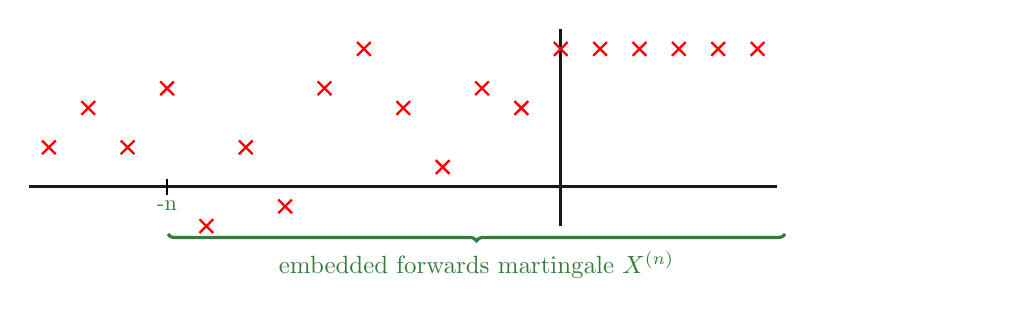
\begin{tikzpicture}
    \tikzset{
      pics/tick/.style args={#1}{code={
        \draw[line width=0.3mm] (0,-#1) -- (0,#1) ;
        },
      }
    }
  \tikzset{
    cross/.pic ={
      \draw[pic actions,rotate=#1,line width=0.3mm]
        (-3.5pt,0) -- (3.5pt,0)
        (0,-3.5pt) -- (0,3.5pt);
    },
  }
    \definecolor{darkgreen}{RGB}{52,125,63}
    %AXIS Y
    \draw[black!90,line width=0.4mm] (4.5,-0.5) -- ++(90:2.5cm);
    %AXIS X 
    \draw[black!90,line width=0.4mm] (-2.25,0) --++(0:9.5cm);
    %TICKS X 
    \draw[black] (-0.5,0) pic {tick={1mm}} node[below,scale=0.8,yshift=-1mm,darkgreen] (n) {-n};

    \foreach \x [count=\i] in {-2,-1.5,...,10} {
      \node (\i) at (\x,0) {} ;
    }
    \foreach \y [count=\i] in {0.5,1,0.5,1.25,-0.5,0.5,-0.25,1.25,1.75,1,0.25,1.25,1,1.75,1.75,1.75,1.75,1.75,1.75}{
      \draw[] ($(\i)+(0,\y)$)pic[red] {cross={45}};
    }
    
    \draw[decorate,decoration={brace,raise=6mm,mirror},draw=darkgreen,line width=0.4mm,scale=0.98] (-0.5,0) -- ++(0:8cm) node[darkgreen,anchor=north,yshift=-7mm,pos=0.5,scale=0.9] (B1) {embedded forwards martingale $X^{(n)}$}; 
  \end{tikzpicture} 
  \end{center}
\end{figure}

	\begin{align*}
		X_k^{(n)} \coloneqq \begin{cases}
					X_{n+k} &: k\in\{0,\cdots , -n \} \\
					X_0 &: k> -n \end{cases}
	\end{align*}
	and the filtrations 
	\begin{align*}
		\cF_k^{(n)} \coloneqq \begin{cases}
								\cF_{n+k} &: k\in\{0,\cdots , -n \} \\
								\cF_0 &: k > -n \end{cases}.
	\end{align*}
	All these processes $(X_k^{(n)})_{k\in\mathbb{N}_0}$ are forwards $(\cF_k^{(n)})_{k\in\mathbb{N}_0}$-martingales (straight from the definition) that are embedded in our backwards martingale. %Note that $\E[X_0\,|\,\cF_0] = X_0$.
	Since $U_{n}[a,b] = U_{-n}^{(n)}[a,b]$, we can use the upcrossing inequality of Lemma \ref{upcrossing_inequality}:
	\begin{align*}
		\E\big[ U_{n}[a,b] \big]=\E\big[ U^{(n)}_{-n}[a,b] \big] \leq \frac{\E\big[(X_{-n}^{(n)}-a)^+\big]}{b-a} = \frac{\E\big[(X_0 - a)^+]}{b-a} \leq \frac{\E[\lvert X_0 \rvert]+ \lvert a \rvert}{b-a}.
	\end{align*}
	Hence, as in the proof of Theorem \ref{as}, the expected total number of upcrossings is finite:
	\begin{align*}
		\E \big[ U[a,b]\big] \overset{\text{MCT}}{=} \lim\limits_{n \to -\infty}\E\big[ U_{n}[a,b] \big] < \infty.
	\end{align*}
	Also as in the proof of Theorem \ref{as} almost sure finiteness of the total upcrossing number through all intervals with rational end-points implies the almost sure existence of the limit $X_{-\infty}:= \lim_{n\to -\infty}X_n$. Since the backwards martingale $(X_n)_{n\in-\N_0}$ is automatically uniformly integrable, Theorem \ref{generalized_DCT} implies the $L^1$-convergence. In particular, $X_{-\infty}$ is almost surely finite. \smallskip
	
	We have to work a bit for the representation $X_{-\infty} = \E[X_0\,|\,\cF_{\infty}]$ of the limit. As usually we verify the two defining properties of conditional expectation:
	\begin{itemize}
		\item For the measurability condition we use Proposition \ref{S2}. It is enough to prove that $\{X_{-\infty} \in (a,b)\}\in  \cF_{-\infty}$ as the open intervals generate the Borel-$\sigma$-algebra. It follows directly from the definition of convergence that $X_{-\infty}\in (a,b)$ if and only if $X_{-n}\in (c,d)$ for all $n$ large enough. In formulas: For all $k\in -\N_0$
		\begin{align*}
			\big\{X_{-\infty}\in (c,d)\big\} =\bigcup_{N=k}^{-\infty} \underbrace{\bigcap_{n=N }^{-\infty} \underbrace{\big\{ X_{n} \in (c,d)\big\}}_{\in \mathcal F_n}}_{\in \cF_{N}\subseteq \mathcal F_k}\in \cF_{k}, 
		\end{align*}
		hence,  $\big\{X_{-\infty}\in (c,d)\big\}\in \cap_{k=0}^{-\infty} \mathcal F_k=\mathcal F_{-\infty}$.
		\item
			Now let $A\in\cF_{-\infty}$. Since $\mathcal F_{-\infty}=\cap_{n\in-\N_0} \cF_{n}$ it holds that $A \in \cF_n$ for all $n\in -\N_0$, so that the expectation condition of conditional expectation holds:
			\begin{align*}
				\E[X_{\infty}\cdot \mathbf 1_A] = \lim\limits_{n\to-\infty}\E[X_{n}\cdot \mathbf 1_A] \overset{X_{n} = \E[X_0|\mathcal F_{n}]}{=} \lim\limits_{n\to-\infty}\E[X_0\cdot \mathbf 1_A] = \E[X_0 \cdot \mathbf 1_A].
			\end{align*}
			The first equality holds as the $L^1$-convergence implies $\E[|X_n-X_\infty|\mathbf 1_A]\leq \E[|X_n-X_\infty|]\to 0$ so that $|\E[X_n\mathbf 1_A]-\E[X_\infty \mathbf 1_A]|\to 0$ by the triangle inequality for expectations.
	\end{itemize}
\end{proof}
As an application we can derive a complement to Proposition \ref{lemma361} but now for decreasing $\sigma$-algebras.
\begin{llemma}
\begin{prop}\label{corollary_354}
	Suppose $Z$ is an integrable random variable and $(\cG_n)_{n\in\mathbb{N}_0}$ a decreasing family of $\sigma$-algebras, then $$\E[Z\,|\,\cG_n] \overset{\text{a.s}/L^1}{\to} \E[Z\,|\,\cG_{\infty}], \quad n\to \infty,$$ where $\cG_{\infty} = \bigcap_{n=0}^{\infty}\cG_n$.
\end{prop}
\end{llemma}
\begin{proof}[Proof]
For $n\in\N_0$ define $X_{-n}= \E[Z\,|\,\cG_n]$ and $\cF_{-n} = \cG_n$. Then $(X_{n})_{n\in-\mathbb{N}_0}$ is an $(\cF_n)$-backwards martingale:
	\begin{itemize}
		\item
			$X_{n}$ is $\cF_{n}$-measurable for all $n\in-\N_0$ as a conditional expectation,
		\item
			$\E[\lvert X_{-n}\rvert ] \overset{\Delta}{\leq} \E \big[ \E [ \lvert Z \rvert \,|\,\cG_n] \big] = \E[\lvert Z \rvert] < \infty$,
		\item		
				$\E[X_{-n}|\cF_{-m}] = \E \big[ \E[ Z\,|\,\cG_n ]\,\big|\,\cG_m \big] \overset{\text{tower prop.}}{=} \E [ Z\,|\,\cG_m] = X_{-m}$ for all $n\leq m$.
	\end{itemize}
	Then Theorem \ref{backwards_martingale_theorem} implies convergence of $X_{-n}=\E[Z|\mathcal G_n]$ for $n\to\infty$ almost surely and in $L^1$ to $$ X_{-\infty} = \E[X_0|\cF_{-\infty}] = \E \big[ \E[Z\,|\,\cG_0]\,|\,\cG_{\infty}\big] \overset{\text{tower}}{=} \E[Z\,|\,\cG_{\infty}].$$
\end{proof}

%Let us summarise Propositions \ref{lemma361} and \ref{corollary_354} in the context of the discussion from Section \ref{sec:gentle}. If $\E[Z|\mathcal F_n]$ is the best approximation of $Z$ using the information of $\mathcal F_n$ it is very natural to ask if the approximations converge whenever the information converges. We do not have a good notion of convergence of information ($\sigma$-algebras) but at least we could interpret increasing or decreasing to a limiting $\sigma$-algebra as convergence of information. The two propositions say that in the approximations converge for increasing or decreasing information. 


\section{Application: Proof of the strong law of large numbers}
We want to finish the chapter on martingales with a typical application. But what is a typical application of martingales? The only common feature of (almost) all famous applications is their magic connection to martingales for questions that seem completely unrelated to martingales\footnote{Check out this article: \href{https://citeseerx.ist.psu.edu/viewdoc/download?doi=10.1.1.215.2970&rep=rep1&type=pdf}{Yuval P\`eres: The Unreasonable Effectiveness of Martingales}}. In that sense, the following proof of the strong law of large numbers is a typical application. Who would guess to derive the law of large number from the backwards martingale convergence theorem?


\begin{ldef}
\begin{deff}\label{tail_sigma_algebra}
	For a stochastic process $Y$ on $(\Omega, \mathcal F, \P)$ one defines the \textbf{tail-}$\mathbf{\sigma}$\textbf{-algebra} $\tau \coloneqq \bigcap\limits_{n=1}^{\infty}\tau_n$, where $\tau_n \coloneqq \sigma(Y_n,Y_{n+1},...)$.
\end{deff}
\end{ldef}
	The tail-$\sigma$-algebra is a sub-$\sigma$-algebra of the underlying $\sigma$-algebra $\cF$ (and also of $\mathcal F_\infty$) containing precisely the events that which do not depend on finitely many of the $Y_n$. Typical examples are events describing convergence properties, finiteness of sum, etc. Here is an example to see a typical computation from the context of the Borel-Cantelli Lemma \ref{BC}. For all $N\in \N_0$
	\begin{align*}
		A := \{ Y_n \geq \lambda \:\:\text{infinitely often}\} = \bigcap\limits_{n=1}^{\infty}\bigcup\limits_{k=n}^{\infty}\{Y_k \geq \lambda \}=\bigcap\limits_{n=N}^{\infty}\underbrace{\bigcup\limits_{k=n}^{\infty}\{Y_k \geq \lambda \}}_{\in\tau_n\subseteq \tau_N}\in \tau_N
	\end{align*}
	by monotonicity of the inner union in $n$. But then $A$ is in the tail-$\sigma$-algebra $\tau$.
\begin{lsatzwichtig}
\begin{theorem}[Kolmogorov $0$-$1$ law]\label{kolmogorov_0_1_law}
	Let $Y_1,Y_2,...$ be independent random variables. Then $\tau$ is trivial, i.e. $$\mathbb{P}(A)\in\{0,1\} \quad\text{ for all }  A\in \tau .$$
\end{theorem}
\end{lsatzwichtig}
\begin{proof}[Proof]
	Take $A\in\tau$ and let $\cF_n = \sigma(Y_1,...,Y_n)$. By the independence assumption $\cF_n$ is independent of $\tau_{n+1}$ for all $n\in\N_0$, and hence also independent of the sub-$\sigma$-algebra $\tau$ (recall the definition \ref{Ka} of independence of $\sigma$-algebras). Using the (forwards) martingale convergence theorem (more precisely Proposition \ref{lemma361}) then yields
	\begin{align*}
	 	\mathbb{P}(A) = \E[\mathbf 1_A] \overset{\text{ind.}}{=} \E[\mathbf 1_A |\cF_n]  \overset{n\to\infty}{\longrightarrow} \E[\mathbf 1_A|\cF_{\infty}] \overset{\tau\subseteq \mathcal F_\infty}{=} \mathbf 1_A \:\: \text{a.s.}
	\end{align*}
	This shows $\mathbb{P}(A) = \mathbf 1_A$ almost surely. The left hand side is a constant and the right hand only takes values $0$ and $1$, that's it.
	\end{proof}
If $X_1,...$ is an iid sequence, then $$A:=\Big\{\omega\in \Omega:\lim_{n\to\infty} \frac{1}{n}\sum\limits_{k=1}^{n}X_k(\omega) \:\text{exists}\Big\}$$ is in the tail-$\sigma$-algebra as changing the values of finitely many summands does not influence the convergence. Using the Kolmogorov $0$-$1$ law we find that convergence in the strong law of large numbers must happen with probability $0$ or $1$. Hence, in order to prove the strong law of large numbers it is enough to prove the probability of convergence cannot be zero and identify the limit.
\begin{lsuperwichtigersatz}
\begin{theorem}[Strong law of large numbers]\label{SLLN}
	Let $X_1,X_2,...$ be an iid sequcence with $\E[\lvert X_1 \rvert ]< \infty$, then
	\begin{align*}
		\frac{1}{n}\sum\limits_{k=1}^{n}X_k \overset{\text{a.s.}}{\longrightarrow} \E[X_1], \:\:\: n\to \infty.
	\end{align*}
\end{theorem}
\end{lsuperwichtigersatz}
\begin{proof}[Proof]
		Here is the main trick that relates the strong law to martingales. Let $S_n \coloneqq \sum\limits_{k=1}^{n}X_k$, then the normalised sum can be written as a backwards martingale:
			\begin{align*}
				\E\big[X_1|\sigma(S_n,S_{n+1},..)\big] = \frac{S_n}{n},\quad \text{for all } n\in\mathbb{N}
			\end{align*}
			To check the claim we use properties of conditional expectations and a trick:
			\begin{align}\label{letztes2}
			\begin{split}
				\E\big[X_1|\sigma(S_n,S_{n+1},..)\big] &= \frac{1}{n} \sum\limits_{k=1}^{n} \E\big[X_k\,|\,\sigma(S_n,S_{n+1},...)\big]\\
										&= \E \Big[ \frac{1}{n}\sum\limits_{k=1}^{n} X_k \,\Big|\,\sigma(S_n,S_{n+1},...)\Big] \\
										&= \E \Big[ \frac{S_n}{n}\,\Big|\,\sigma(S_n,S_{n+1},...)\Big]
										= \frac{S_n}{n}.
								\end{split}
			\end{align}
			Only the first equality needs extra explanation, but we have already seen the argument in Example \ref{so}. The intuitive reason is the same that was mentioned in the example: Given the values of all sums after $n$ the best guess for the first $n$ summands is the same for each summand as they are iid and equally influence the values of the sums. Writing a formal proof is a bit messy.	Using property (x) of Theorem \ref{cond_properties} it suffices to check
			\begin{align}\label{letztes}
				\E[X_1\mathbf 1_A]=...=\E[X_n\mathbf 1_A],\quad \forall A\in \sigma(S_n,...)
			\end{align}
			and then take the average. To check \eqref{letztes} note that the iid assumption gives $\E[F(X_1,...)]=\E[F(X_{\sigma(1)},...)]$ for all finite permutations and all bounded measurable functions. Choosing $A\in \sigma(S_n,...)$ there is a measurable mapping $h$ such that $\mathbf 1_A=h(S_n,...)$. Hence, there is also a measurable mapping $g$ such that $\mathbf 1_A=g(X_1,...)$ and $g$ does not change by permuting the first $n$ entries. Using $F(x_1,...)=x_1 g(x_1,...)$ and the permutation that only exchanges two integers yields \eqref{letztes}.\smallskip
			
			So how do we finish the proof? We first show that $\liminf\limits_{n\to\infty}\frac{S_n}{n}$ is almost surely constant. To see this first note that, for all $\lambda\in \R$,
			\begin{align*}
				\Big\{ \liminf\limits_{n\to\infty}\frac{1}{n}\sum\limits_{k=1}^{n}X_k \leq \lambda \Big\} = \Big\{ \frac{1}{n}\sum\limits_{k=1}^{n}X_k \leq \lambda \text{ i.o.}\Big\} \in \tau.
			\end{align*}
			Thus, by Proposition \ref{S2}, the random variable $\liminf\limits_{n\to\infty}\frac{S_n}{n}$ is measurable with respect to the tail-$\sigma$-algebra. Now we use the following simple fact:
			\begin{luebung}
				If $\mathcal A$ is a trivial $\sigma$-algebra on $\Omega$, then all $\mathcal A$-measurable random variables are constant.
			\end{luebung}




			Applying Proposition \ref{corollary_354} with $G_n \coloneqq \sigma(S_n,S_{n+1},...)$ to the left hand side of \eqref{letztes2} shows that the limits of both sides exist almost surely. If the limit of the right hand side exists it equals the limit inferior which, as we have seen above, is constant. Hence, both sides of
			\begin{align*}
				\lim\limits_{n\to\infty}\frac{1}{n}\sum\limits_{k=1}^{n}X_k = \E \big[ X_1\big | \cG_\infty\big]
			\end{align*}
			are constant. But then Theorem \ref{cond_properties} (ix) implies that the right hand side equals $\E[X_1]$ almost surely. That's it!
\end{proof}
Here is a question: Do we really need the iid assumption in the proof of the strong law of large numbers? Actually, not quite. Ommitting the use of Kolmogorov's 0-1 law gives the law of large numbers for so-called exchangeable sequences (finite permutations do not change the distribution of the sequence). In that case the proof only gives the almost sure onvergence of the normalised sum towards the (non-constant) random variable $\E[X_1|\mathcal G_\infty]$. This, and more on exchangeable sequences can be found in a beautiful article of Kingman \footnote{J. F. C. Kingman, "{}Uses of Exchangeability", Annals of Probability, 1978,
Vol. 6, pp. 183-197}.


%Now towards the final application: Let $\xi_1,\xi_2,...$ be iid random variables with values in a measurable space $(E,\varepsilon)$ and $F\colon E^{\mathbb{N}}\to \mathbb{R}$ $\big( \varepsilon^{\otimes \mathbb{N}}, \cB(\mathbb{R})\big)$-measurable. Then $F$ is called symmetric if $F(X_1,X_2,...) = F(X_{\pi_{(1)}},X_{\pi_{(2)}},...)$ for all finite permutation on $\mathbb{N}$, i.e. $\pi\colon\mathbb{N}\to\mathbb{N}$ bijective with $\pi(k)\neq k$ only finitely often.

%\begin{theorem}[Hewitt-Savage]\label{Hewitt_Savage}
%	If $\xi_1,\xi_2,...$ aare iid and $F$ is symmetric and bounded, then the random variable $F(\xi_1,\xi_2,...)$ is a.s. a constant.
%\end{theorem}
%\begin{example1}
%	Let $\xi_1,\xi_2,...$ be iid and $S_n = \sum\limits_{k=1}^{n}\xi_k$ the random walk with step size distribution $\xi_1$ and for ssome $B\in\cB(\mathbb{R})$
%	\begin{align*}
%		F(X_1,...) = \mathbf 1_{\# \{n\geq 1 \colon \sum\limits_{k=1}^{n}X_k \in B\}=\infty}
%	\end{align*}
%	is symmetric. Therefore, $\mathbb{P}\big( \# \{ n\geq 1 \colon \sum\limits_{k=1}^{n}X_k \in B\}=\infty \} \big) \in \{0,1\}$.
%\end{example1}

%\begin{proof}
%	Let $\cF_n = \sigma (\xi_1,\xi_2,...,\xi_n)$ and $\cG_n = \sigma ( \xi_{n+1},...)$. Denote by $Y \coloneqq F(\xi_1,\xi_2,...)$ and $X_n = \E[Y\,|\,\cF_n]$, $Z_n = \E[Y\,|\,\cG_n]$. Since $X_n$ is a Doob martingale (closed martingale)
%	\begin{align}\label{eq_4}
%	X_n \overset{\text{a.s./}\cL^1}{\longrightarrow} X_{\infty} = \E[Y\,|\,\cF_{\infty}] \overset{\text{meas.}}{=} Y
%	\end{align}
%	as $n\to\infty$. By \ref{corollary_354} we also have that $Z_n \overset{\text{a.s./}\cL^1}{\longrightarrow} \E[Y\,|\,\cG_{\infty}] = \E[Y]$. Now fix $\varepsilon >0$. Then there is $N\in\mathbb{N}$ large enough with $$ \E[\lvert X_n - Y \rvert ] < \varepsilon,\: \E\big[\lvert Z_n - \E[Y] \rvert \big] < \varepsilon \:\: \forall n\geq N$$
%By the factorisation lemma $X_n = g_n(\xi_1,...,\xi_n)$ for some measurable $g_n$. Then \ref{eq_4} can be rewritten as 
%	\begin{align}\label{eq_5}
%		\E\big[ \lvert g_n(\xi_1,...,\xi_n)-Y \rvert \big] < \varepsilon \:\:\: \forall n \geq N
%	\end{align}
%	Now we use the symmetry of $F$:
%	\begin{align*}
%		Y = F(\xi_1,...) = F(\xi_{n+1},...,\xi_{2n},\xi_1,...,\xi_n,\xi_{2n+1},...)
%	\end{align*}
%	and that $(\xi_1,\xi_2,...)$ has the  same distribution as $(\xi_{n+1},...,\xi_{2n},\xi_1,...,\xi_n,\xi_{2n+1},...)$ to deduce from \ref{eq_5}
%	\begin{align*}
%		\E\big[ \lvert g_n(\xi_{n+1},...,\xi_{2n})- Y \rvert \big] < \varepsilon
%	\end{align*}
%	and from this also
%	\begin{align*}
%		\E \big[ \lvert Z_n - g_n(\xi_{n+1},...,\xi_{2n})\rvert \big] \overset{\text{meas.}}&{=} \E \big[ \lvert \E [ Y\,|\,\cG_n ] - \E[g_n(\xi_{n+1},...,\xi_{2n})\,|\,\cG_n]\lvert\big] \\
%			&\leq \E \big[ \E[ \lvert Y - g_n(\xi_{n+1},...,\xi_{2n}) \rvert \,|\,\cG_n] \big] \\
%			&= \E [  \lvert Y - g_n(\xi_{n+1},...,\xi_{2n}) \rvert ]\\
%			&< \varepsilon
%	\end{align*}
%	Everything combined gives for $n\geq N$:
%	\begin{align*}
%		&\E \big[ \lvert Y - \E[Y] \rvert \big] \\
%		&\leq \E \big[ Y - g_n (\xi_{n+1},...,\xi_{2n}) \rvert \big] + \E \big[ \lvert g_n(\xi_{n+1},...,\xi_{2n}) - Z_n \rvert \big] + \E \big[ \lvert Z_n - \E[Y] \rvert \big] \\
%		&< 3 \varepsilon
%	\end{align*}
%	Since $\varepsilon$ was arbitrary $\E[Y] = Y$ a.s., so $Y = F(\xi_1,\xi_2,...)$ is a.s. constant.
%\end{proof}
%\endinput



	% !TeX spellcheck = en_US
\chapter{Convergence of Measures}
	\marginpar{\textcolor{red}{Lecture 11}}
In this chapter the technical tools for proving Donsker's famous invariance principle will be developed. This main result of Chapter \ref{sec:BM} will be to prove weak convergence of scaled random walks with second moment jumps towards the Brownian motion. But what does weak convergence of a sequence of stochastic processes mean? The convergence will be defined to be weak convergence of the processes interpreted as path-valued random variables. We already met the notion of weak convergence of real-valued random variables in Section \ref{sec:konvergenz}, in this chapter weak convergence will be generalised to much more general state spaces. To do so, a bit of Functional Analysis needs to be combined with measure theory and a bit of probability. Along the way we will also prove a couple of theorems on the characterisation of random variables through moments. 


\section{A bit of topology, measure, and integration theory}
To get started let us recall from analysis some topological concepts that will lead us naturally to general Borel-$\sigma$-algebras. We will always work with metric or normed spaces $E$, metrics will typically be denoted by $d$ and norms $||\cdot||$. A central object of basic topology are open and closed sets:
\begin{ldef}
\begin{deff}
	Suppose $(E,d)$ is a metric space and 
	\begin{align*}
		B_\varepsilon(x):=\{y\in E: d(x,y)<\varepsilon\},\quad \varepsilon>0,
	\end{align*}
	are the $\varepsilon$-balls around $x$. 
	\begin{itemize}
		\item $A\subseteq E$ is called \textbf{open} if for all $x\in A$ there is some $\varepsilon>0$ such that $B_\varepsilon(x)\subseteq A$.
		\item $A\subseteq E$ is called \textbf{closed} if $A^c$ is open.
	\end{itemize}	
	The set of all open sets is also the \textbf{topology} of $E$ and denoted by $\tau$. Any open set containing a ball $B_\varepsilon(x)$ is called an (open) \textbf{neighbourhood} of $x$.
	\begin{itemize}
		\item $A\subseteq E$ is called \textbf{bounded} if there is some $r>0$ such that $d(x,y)\leq r$ for all $x,y\in A$.
	\end{itemize}
\end{deff}
\end{ldef}
To study various properties of subsets of metric spaces very quickly one needs to think about more fine properties. Since there are many equivalent ways of redefining the following definitions it is likely that you might have seen different notions in your basic analysis lectures.
%From analysis the concept of open sets in a metric or normed space should be familiar, those were defined using the balls of the metric (or the norm). In fact, many theorems from analysis can be proved in a more general setting in which the open sets are not defined through balls but just using axioimatic properties.
%\begin{ldef}
%\begin{deff}
%	Let $E \neq \emptyset$ and $\tau \subseteq \cP(E)$. Then $\tau$ is called a \textbf{topology} on $E$ if
%	\begin{itemize}
%		\item
%			$\emptyset,E \in \tau$,
%		\item Finite intersection stability:
%			$$A,B\in\tau \:\Rightarrow\: A\cap B \in \tau,$$
%		\item Union stability for arbitrary index set $I\neq \emptyset$:
%			$$A_i \in \tau \:\: \forall i \in I\:\Rightarrow\: \bigcup\limits_{i\in I} A_i \in \tau.$$
%	\end{itemize}
%	The pair $(E,\tau)$ is called a \textbf{topological space}. Sets $A\in E$ are called \textbf{open sets}, their complements in $E$ are called \textbf{closed sets}.
%\end{deff}
%\end{ldef}
%Note that topologies are a bit similar to $\sigma$-algebras, both are families of subsets of some base set that satisfy axiomatic properties for intersections and unions. In $\sigma$-algebras we speak of events, in topologies of open sets. Many arguments are somewhat similar, even though topologies and $\sigma$-algebras do not have much in common and are used for completely different purposes. Just as for $\sigma$-algebras there are always the two trivial topologies $\tau=\{\emptyset, E\}$ and $\tau=\mathcal P(E)$. Here is an example of a properties that is proved in the same ways for topologies and $\sigma$-algebras:
%\begin{luebung}
%	If $(\tau_j)_{j\in J}$ is an arbitrary family of topologies, then $\cap{j\in J} \tau_j$ is a topology. Unions of topologies are generally not topologies.
%\end{luebung}
%In almost all situations we will consider a metric space $(E,d)$ and the topology of open sets induced by the metric. Recall that a subset $A$ of a metric space is called open if for all $x\in A$ there is some $\varepsilon>0$ such that $B_\varepsilon(x)\subseteq A$, where the balls are defined by $B_\varepsilon(x):=\{y\in E: d(x,y)<\varepsilon\}$. If we are extremely lucky the metric space is actually a normed space with the metric $d(x,y)=||x-y||$ induced by the norm. Please quickly check your analysis notes to recall properties that hold in metric spaces and normed spaces.\smallskip
\begin{ldef}
\begin{deff}
	Suppose $(E,d)$ is a metric space and $A \subseteq E$. 
	\begin{itemize}
		\item
			$x\in A$ is called an \textbf{inner point} if there is $\varepsilon>0$ such that $B_\varepsilon(x)\subseteq A$.
		\item
			The set of inner points of $A$ is denoted by $\dot{A}$ and is called \textbf{interior of A}.
		\item
			The \textbf{closure} $\bar{A}$ is the smallest closed set containing $A$ (the intersection of all closed sets containing $A$).
		\item
			$\partial A \coloneqq \bar{A}\text{\textbackslash}\dot{A}$ is called the \textbf{boundary} of $A$.
		\item
			$A$ is called \textbf{dense} in $E$ if $\bar{A} = \bar{E}$.
	\end{itemize}
\end{deff}
\end{ldef}
Please keep in mind the important facts that arbitrary unions of open sets are open and finite intersections of open sets are open. The empty set and the entire space are both open and closed.
% For topological spaces the $\varepsilon$-$N$-formulation does not exist so we use the more abstract formulation to define convergence:
%\begin{ldef}
%\begin{deff}
%	A sequence $(x_n)_{n\in\mathbb{N}} \subseteq E$ converges in $(E,\tau)$ towards $x$ if for every open set $\cO\in \tau$ containing $x$ there is some $N\in\mathbb{N}$ such that $x_n \in \cO$ for all $n \geq N$.
%\end{deff}
%\end{ldef}\begin{ldef}
\begin{ldef}
\begin{deff}
Suppose $(E,d)$ is a metric space.
\begin{itemize}
	\item	A sequence $(x_n)_{n\in\mathbb{N}} \subseteq E$ \textbf{converges} in $E$ towards $x$ if $\lim_{n\to\infty} d(x_n,x)=0$, i.e. for every $\varepsilon$ there is some $N\in\mathbb{N}$ such that $d(x_n,x)<\varepsilon$ for all $n \geq N$.
	\item	A sequence $(x_n)_{n\in\mathbb{N}} \subseteq E$ is called a \textbf{Cauchy-sequence} in $E$ if for all $\varepsilon>0$ there is some $N\in \N$ such that $d(x_n,x_m)<\varepsilon$ for all $n,m\geq N$. 
	\item If all Cauchy-sequences in $E$ converge, then $E$ is called \textbf{complete}.
\end{itemize}
\end{deff}
\end{ldef}
%Often one sees the the definition of convergence in the equivalent notion $x_n\in B_x(\varepsilon)$ instead of $d(x_n,x)<\varepsilon$ or with $x_n\in \mathcal O$ for all neighbourhoods of $x$.\smallskip


This section is mostly about convergence so let us recall the important connection of closeness and convergence. A set $A$ is closed if and only if all converging sequences $(x_n)\subseteq A$ converge to some $x\in A$. Formulated differently, $\bar A$ consists precisely of those elements which are the limits of sequences in $A$. Just check yourself some examples for intervals in $\R$! \smallskip

%It is not so clear how to extend the notion of a Cauchy sequence to general topological spaces. This is only done for topological spaces carrying additional structure, for example metrizable topological spaces:
%\begin{ldef}
%\begin{deff}
%	A topological space $(E,\tau)$ is called \textbf{metrizable} if there is a metric $d$ on $E$ so that $\tau$ coincides with the open sets defined through the \textbf{open balles} $B_{\varepsilon}(x) \coloneqq \{ y\in E\,|\, d(x,y)<\varepsilon \}$ of $d$. A metrizable topological space is called \textbf{complete} if all Cauchy sequences converge in $E$.
%\end{deff}
%\end{ldef}
%Not all topologies are metrizable! In such cases obvious properties of convergence that you are used to from basic analysis can be wrong. As an example, the uniqueness of limits of sequences holds in metric spaces (hence, in metrizable topological spaces) but can fail in non-metrizable metric spaces. 
%\begin{luebung}
%	Suppose $E$ is some non-empty set and $\tau=\{\emptyset, E\}$ is the trivial topology. What does it mean that a sequence $(x_n)_{n\in\N}\subseteq E$ converges? Are the limits of converging sequences unique?
%\end{luebung}
In the discussion of conditional expactations $\E[X|Y]$ we have strongly used that $\R$ contains the countable dense subset $\Q$. Once we combine general metric spaces with measures theory it won't come as a surprise (think of the definition of a measure and $\sigma$-algebras) that the existence of countable dense subsets should be useful.
%\begin{ldef}
%\begin{deff}
%	If $(E,d)$ is a metric space, then we define for $A,B\subseteqq E$.
%	\begin{itemize}
%		\item $d(x,B) = \inf\{ d(x,y)\,|\,y\in B \}$
%		\item $d(A,B) = \inf\{ d(x,y)\,|\, x\in A, y\in B \}$
%	\end{itemize}
%\end{deff}
%\end{ldef}



\begin{ldef}
\begin{deff}
	A metric space $(E,d)$ is called \textbf{separable} if there is a countable and dense subset of $E$.
\end{deff}
\end{ldef}
Here is a small but useful fact from topology. A metric space $(E,d)$ is separable if and only if the topology $\tau$ has a countable base $\mathcal B$. A  base $\mathcal B$ is a subset of open sets such that all open sets can be written as a union of sets from the base. The concept of a base is a bit similar to a generator of a $\sigma$-algebra but somewhat simpler as we are only allowed to take countable unions of events in $\sigma$-algebras but arbitrary unions of open sets for a base.
\begin{luebung}
	The set of all intervals with rational end-points is a countable base of the topology of $\R$ induced by the usual norm.
\end{luebung}
There is a special class of metric spaces that turned out to be most useful in Functional Analysis and probability theory. This is the typical setting in which the general theory of Markov processes can be developed.
\begin{ldef}
\begin{deff}
	A \textbf{Polish metric space} is a  complete and separable metric space.
\end{deff}
\end{ldef}
The word Polish in the definition honours the school of Polish mathematicians from the 20th century that was responsible for the development of almost all tools of Functional Analysis. There are a few prime examples of Polish metric spaces that we will encounter again and again:
\begin{align*}
	(\R,|\cdot|),\quad (\R^d, |\cdot|),\quad (\C,|\cdot|),\quad\text{and}\quad (C([0,1]),||\cdot||_\infty),
\end{align*}
where $C([0,1])$ are the continuous real-valued functions on $[0,1]$. 
\begin{ldef}
\begin{deff}
	Suppose $(E,d)$ is a metric space and $A \subseteq E$. 
	\begin{itemize}
		\item
			$A$ is called \textbf{compact} if every covering of $A$ by open sets has a finite subcovering, $A$ is called \textbf{sequentially compact} if every sequence in $A$ has a subsequence that converges to a limit in $A$.
					\item
			$A$ is called \textbf{relatively compact} if $\bar{A}$ is compact, $A$ is called \textbf{relatively sequentially compact} if all sequences in $A$ have a subsequence with limit in $\bar{A}$.
%		\item 
%			$E$ is called \textbf{locally compact} if each point has an open neighborhood whose closure is compact.
	\end{itemize}
\end{deff}
\end{ldef}
Different characterisations of compactness have been discussed for $(\R^d,|\cdot|)$ in analysis, in particular, compactness and sequential compactness are equivalent and compact sets are precisely the closed and bounded sets (Heine-Borel Theorem). The Heine-Borel equivalence fails in most other metric spaces but we still know from analysis (check it!) that
\begin{align*}
	A\text{ is (relatively) compact}\quad& \Longleftrightarrow \quad A\text{ is (relatively) sequentially compact},
\end{align*}
holds in all metric spaces. In complete metric spaces a more general version of Heine-Borel can be formulated using the concept of total boundedness:
\begin{ldef}
\begin{deff}
	A set $A\subseteq E$ is called \textbf{totally bounded} if for all $\varepsilon>0$ there are finitely many points $x_1,...,x_n\in A$ with $A \subseteq \bigcup\limits_{k=1}^n B_{\varepsilon}(x_k)$. 
\end{deff}
\end{ldef}	
Using the triangle inequality it is easy to see that totally bounded sets are always bounded, i.e. are covered by a large single ball. It is not generally the case that bounded sets are also totally bounded.
\begin{luebung}
	Check that boundedness and totally boundedness are equivalent in $(\R^d,|\cdot|)$ but are not equivalent in all infinite sets with the discrete metric (i.e. $d(x,y)=\frac{1}{2}$ for all $x\neq y$).
\end{luebung}
We will see later that totally-bounded and bounded are not the same in $(C([0,1],||\cdot||_\infty)$.\footnote{nicht vergessen}\smallskip

\begin{llemma}
\begin{prop}
	Suppose $(E,d)$ is a complete metric space and $A\subseteq E$, then
	\begin{align*}
		A\text{ is compact}\quad& \Longleftrightarrow \quad A\text{ is closed and totally bounded}.
	\end{align*} 
	\end{prop}
\end{llemma}
\begin{proof}[Proof]
	 %Let us first remind ourselves of a quick sketch of the complicated direction in $\R$. If a sequence lies in a bounded set $A$, let's say $A\subseteq [-N,N]$, then infinitely many elements must be (at least) in one of the two halfs of the interval. Take that half and divide it into two again, one of them must contain infinitely many elements of the sequence. Proceeding like that we can track down a converging subsequence. If $A$ is additionally closed, then the limit is in $A$. Hence, every sequence in a bounded and closed set $A$ has a converging subsequence, thus, $A$ is sequentially compact. Looking carefully at that argument we used that intervals in $\R$ are totally bounded, we covered $[-N,N]$ by finitely many intervals of shrinking size. It is instructive to keep the idea in mind to understand how one typically generalises proofs to Polish spaces.\smallskip
"$\Rightarrow$": $A$ totally bounded follows from the compactness definition by covering $A$ with $\varepsilon$-balls around all elements, $A$ closed follows from sequential compactness since in metric spaces all subsequences converge to the same limit as their convergent sequences.\smallskip

"$\Leftarrow$": Take a sequence $(x_n) \subseteq A$. For each $m\in\mathbb{N}$ take a finite covering $B_{\frac{1}{m}}(y_1^m),...$ of $A$. By the finiteness there must be a subsequence which lies eventually in one of the balls $B_1(y_k^1)$. Similarly, from this subsequence we extract a further subsequence which lies eventually in one of the $B_{\frac{1}{2}}(y_k^2)$. A diagonal argument gives a subsequence with $x_n \subseteq B_{\frac{1}{n}}(y_k^n)$. This is Cauchy and converges by completeness. Hence, $A$ is sequentially compact.
\end{proof}
It is not too hard to come up with counter examples to the second equivalence in non-complete spaces. For instance, take the normed space $(\mathbb{Q},|\cdot| )$ and $A = (-\sqrt{2},\sqrt{2})\cap \mathbb{Q}$. Then $A$ is closed, totally bounded but not compact.\smallskip


As always in mathematics we are interested in the natural mappings between objects, mappings that respect the structure of the objects. For $\sigma$-algebra these were the measurable mappings, for metric spaces these are the continuous mappings:
\begin{ldef}
\begin{deff}
	A mapping between two metric spaces $(E,d_E)$ and $(F,d_F)$ is called \textbf{continuous} if preimages of all open sets in $F$ are open in $E$. We use the notation
	\begin{itemize}
		\item $C(E,F)\coloneqq  \{ f\colon E \to F \,|\, f \text{ continuous} \}$
		\item
			$C(E) \coloneqq \{ f\colon E \to \mathbb{R} \,|\, f \text{ continuous} \}$
		\item
			$C_b(E) \coloneqq \{ f\colon E \to \mathbb{R} \,|\, f \text{ continuous, bounded}\}$
		\item
			$C_c(E) \coloneqq \{ f\colon E \to \mathbb{R} \,|\, f \text{ continuous, compact support}\}$
	\end{itemize}
	A compactly supported function is defined as in basic analysis as a function such that $\{x\in E: f(x)=0\}$ is contained in a compact set.
\end{deff}
\end{ldef}
Recall that there are other equivalent ways of defining continuity via $\varepsilon$-$\delta$ formalism
\begin{align*}
	\forall \varepsilon>0 \exists \delta>0: d_E(x,y)<\delta \,\Rightarrow\, d_F(f(x),f(y))<\varepsilon
\end{align*}
and sequences
\begin{align*}
	x_n\to x, \,n\to\infty\quad \Longrightarrow\quad f(x_n)\to f(x), \, n\to\infty.
\end{align*}
We will always use the most convenient formulation. Here is a not so simple exercise:
\begin{luebung}
	$(C_b([0,\infty)), ||\cdot||_\infty)$ is not separable but $(C_c([0,\infty)), ||\cdot||_\infty)$ is separable.
\end{luebung}
Now we come to the fun part, extending the concepts from measure theory on the Borel-$\sigma$-algebra of $\R$ to general metric spaces. Recall that $\mathcal B(\R)$ was defined to be the smallest $\sigma$-algebra containing all open sets (or closed sets, or intervals, etc.), hence, it is quite clear how we should proceed for general metric spaces.
\begin{ldef}
\begin{deff}
	For a metric space $(E,d)$ we call 
	\begin{align*}
		\cB(E)=\sigma(\{O\subseteq E: O\text{ open}\})
	\end{align*}	
		 the \textbf{Borel-}$\mathbf{\sigma}$-\textbf{algebra} on $E$.
\end{deff}
\end{ldef}
Of course, since $\sigma$-algebras are closed under taking complements $\mathcal B(E)$ is also generated by all closed sets. It is also instructive to check the following exercise to link topology and measure theory. The proof is precisely the same that shows that $\mathcal B(\R)$ is also generated by all intervals.
\begin{luebung}
	If $(E,d)$ is separable, then $\mathcal B(E)=\sigma(\{B_\varepsilon (x):x\in E, \varepsilon >0\}).$
\end{luebung}
Measurable mappings between two metric spaces will always be with respect to the corresponding Borel-$\sigma$-algebras. Not surprisingly we will call such measurable mappings \textbf{Borel-measurable}. From the definition of continuity and Proposition \ref{S2} it is clear that all continuous functions between metric spaces are Borel-measurable.
\begin{ldef}
\begin{deff}
	Let $(E,d)$ be a metric space, then
	\begin{itemize}
		\item
			$\cM_f(E) \coloneqq \cM_f \coloneqq \{ \mu: \mu \text{ is a finite measures on}\: \cB(E) \}$
		\item
			$\cM_1(E) \coloneqq \cM_1 \coloneqq \{\mu:  \mu \text{ is a probability measures on}\: \cB(E) \}$
		\item
			$\cM_{\leq 1}(E) \coloneqq \cM_{\leq 1} \coloneqq \{ \mu:\mu\text{ is a sub-probability measures one}\: \cB(E) \}$
	\end{itemize}
\end{deff}
\end{ldef}
After all these definition let us prove a first proposition on measures on Polish spaces. Before checking the proof have a quick thought how you would prove the statement on $\mathcal B(\R)$ using continuity of measures with $(-n,n)$ and you will immediately appreciate a useful property of $\R$, namely, to be able to fill $\R$ from the inside by increasing intervals.
\begin{llemma}
\begin{prop}\label{prop_4120}
	Suppose $(E,d)$ is Polish and $\mu \in \cM_f$. Then, for all $\varepsilon > 0$, there is a compact set $K$ with $\mu(K^c)<\varepsilon$.
\end{prop}
\end{llemma}
\begin{proof}[Proof]
	The trick is to replace the increasing intervals $(-n,n)$ in $\R$ by the right substitute and then try to argue with continuity of measures. Let $x_1,x_2,...$ the countable dense subset of $E$ and $n\in\mathbb{N}$. Then $E = \bigcup\limits_{k=1}^{\infty} B_{\frac{1}{n}}(x_k)$ for all $n\in\N$. Using continuity of measures (this needs $\mu\in \mathcal M_f$, compare Theorem \ref{S1}) fix $N_n \in \mathbb{N}$ with 
	\begin{align*}
		\mu \Big( E \text{\textbackslash} \bigcup\limits_{k=1}^{N_n}B_{\frac{1}{n}}(x_k)\Big) < \frac{\varepsilon}{2^n}
	\end{align*}
	Now define $A \coloneqq \bigcap_{n=1}^{\infty} \bigcup_{k=1}^{N_n}B_{\frac{1}{n}}(x_k) \in\cB(E)$. $A$ is totally bounded as $A\subseteq \bigcup_{k=1}^{N_n} B_{\frac{1}{n}}(x_k)$ for all $n\in\N$, hence, $\bar{A}$ is compact as $E$ is complete. If we choose $K \coloneqq \bar{A}$, then
	\begin{align*}
		\mu (K^c) = \mu (E \text{\textbackslash} K ) 
				\overset{\text{mon.}}{\leq} \mu (E \text{\textbackslash} A ) 
				= \mu \bigg( \bigcup_{n=1}^{\infty} \bigcap_{k=1}^{N_n}B_{\frac{1}{n}}^c (x_k) \bigg).
	\end{align*}			
	Using sub-additivity we can continue the chain of inequalities with
	\begin{align*}
				\sum\limits_{n=1}^{\infty} \mu \bigg( \bigcap\limits_{k=1}^{N_n} B_{\frac{1}{n}}^c (x_k) \bigg) 
				= \sum\limits_{n=1}^{\infty} \mu \bigg( E \text{\textbackslash} \bigcup\limits_{k=1}^{N_n} B_{\frac{1}{n}}(x_k) \bigg)
				\leq \sum\limits_{n=1}^{\infty}\frac{\varepsilon}{2^n}
				= \varepsilon
	\end{align*}
	which finishes the proof.
\end{proof}
We can now turn towards a crucial topic of this chapter. Is it possible to characterise measures using only integrals over certain functions?
\footnote{brauchen wir wirklich $\cM_f$?}
\begin{ldef}
\begin{deff}
	Let $(E,d)$ a metric space and $F \subseteq \cM_f(E)$ a family of measures. A family $C$ of measurable mappings $E \to \mathbb{R}$ is called \textbf{\smash{separating family} for $F$} if for all $\mu,\nu \in F$
	\begin{align*}
		\int_E f\dint \mu = \int_E f\dint \nu \:\:\: \forall f \in C \cap L^1(\mu)\cap L^1(\nu)\: \Rightarrow \: \mu = \nu
	\end{align*}
\end{deff}
\end{ldef}
The most simplistic (and least useful) family is the family of all measurable indicator functions $C:=\{\mathbf 1_A: A\in \mathcal B(E)\}$ which trivially separates all families of measures as $f=\mathbf 1_A$ yields
 $$\nu(A) = \int_E f\dint \nu = \int_E f \dint \mu = \mu (A).$$
% A slightly smaller example is the family of all indicators on a $\cap$-stable generator of $\mathcal B(E)$ that separates all finite measures by Theorem \ref{Dynkin-Folgerung}. 
Since the set of all indicators on measurable set is equally big as the Borel-$\sigma$-algebra there is a big desire to finde more approachable sets such as all exponential functions or all polynomial functions. To understand the background of separating families in probability let us recall Theorem \ref{WT}, which in Stochastik 1 we stated without a proof:
\begin{align*}
	\int_\R e^{t x} \dint \P_X(x)=M_X(t)=M_Y(t)= \int_\R e^{t x} \dint \P_Y(x),\quad \forall t\in [-\varepsilon,\varepsilon]\quad \Longrightarrow \quad \P_X=\P_Y.
\end{align*}
If we reformulate, Theorem \ref{WT} states that exponential functions are separating for probability measures with exponential moments. A more precise statement will be proved towards the end of this chapter.\smallskip

 During the course of this chapter we will get to know which families of measurable mappings are separating for different classes of measures. We start with a first smaller step and prove that Lipschitz continuous functions are separating for finite measures.
\begin{ldef}
\begin{deff}
	Let $(E,d_E)$ and $(F,d_F)$ be metric spaces.
	\begin{itemize}
		\item
			$f\colon E \to F$ is called Lipschitz continuous (with constant $K$) if 
			\begin{align*}
				d_F \big( f(x),f(y) \big) \leq K \cdot d_E(x,y) \:\:\: \forall x,y\in E
			\end{align*}
		\item
			$\text{Lip}_K(E,F) \coloneqq \{ f\colon E\to F \,|\, \text{Lipschitz with constant }K \}$
		\item
			$\text{Lip}(E,F) \coloneqq \{ f\colon E\to F \,|\, \text{Lipschitz}\}$
		\item
			$\text{Lip}_K(E) \coloneqq \text{Lip}_K(E,\mathbb{R})$
		\item $\text{Lip}(E) \coloneqq \text{Lip}(E,\mathbb{R})$
	\end{itemize}
\end{deff}
\end{ldef}
As promised the Lipschitz continuous functions are separating the finite measures on $E$. In fact, the same proof also shows that bounded and compactly supported continuous functions separate $\mathcal M_f(E)$. 
\begin{lsatzwichtig}
\begin{prop}\label{theorem_4124}
	In metric spaces $\text{Lip}_1(E)$, $C_b(E)$, and $C_c(E)$ are separating for $\cM_f(E)$.
\end{prop}
\end{lsatzwichtig}
\begin{proof}[Proof]
	First of all, note that $f\in \text{Lip}_K(E)$ implies $\frac{1}{K} f \in \text{Lip}_1(E)$. Hence, if we assume $\int_E f\dint \mu=\int_E f\dint \nu$ for all $f\in \text{Lip}_1(E)$ we can also use 
	\begin{align}\label{Lip}
			\int_E f\dint \mu = \int_E f\dint \nu,\quad \forall f \in \text{Lip}(E),
	\end{align}
	whenever the integrals are finite. We will show that \eqref{Lip} implies $\nu(A)=\mu(A)$ for all $A$ closed. Since the closed sets form an $\cap$-stable generator of $\mathcal B(E)$ we can then deduce $\mu=\nu$ from Theorem \ref{Dynkin-Folgerung} (this uses the finiteness of $\mu$ and $\nu$).\smallskip
	
	We now fix $\mu, \nu\in \mathcal M_f(E)$ and $A\subseteq E$ closed. Then define the functions
	\begin{align*}
		f_A^{\varepsilon}(x) \coloneqq \Big( 1 - \frac{1}{\varepsilon} \cdot d(x,A) \Big)^+,\quad x\in E, \varepsilon>0,
	\end{align*}
	with $d(x,A)=\inf\{d(x,y):y\in A\}$. 
			\begin{figure}[h]
			\begin{center}
				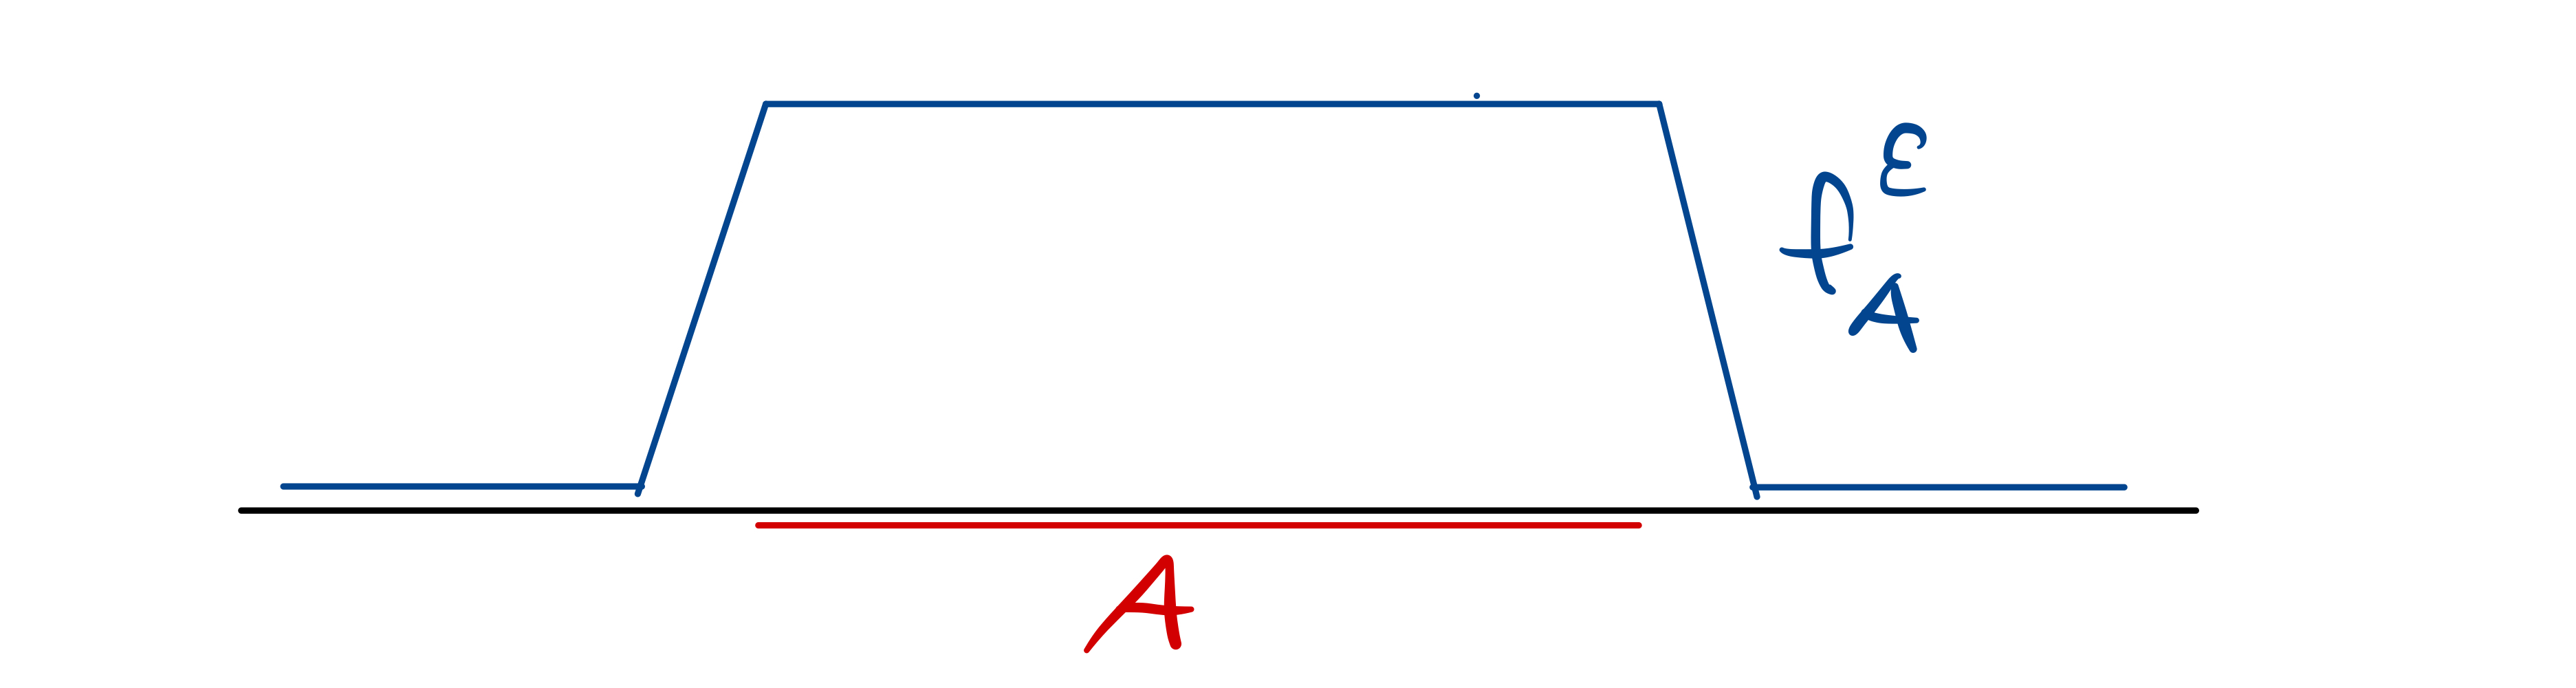
\includegraphics[scale=0.07]{f.jpeg}
			\end{center}
			\vspace{-9mm}
			\end{figure}	
	Remember from basic analysis (or quickly check yourself by using that $\bar A$ are precisely the limits of sequences in $A$) that $d(x,A)=0$ if and only if $x\in \bar A$. The functions $f_A^\varepsilon$ have the following properties:	
			\begin{itemize}
				\item $f_A^{\varepsilon} = 1$ on A
%				\item $f_A^{\varepsilon}(x) = 0$ if $d(x,A)\geq \varepsilon$
				\item $f_A^{\varepsilon} \to \mathbf 1_A$, because for closed sets $d(x,A)=0$ if and only if $x\in A$,
				\item $f_A^{\varepsilon} \leq 1$
			\end{itemize}
			Since the idea of using the functions $f_A^\varepsilon$ is (almost) the entire point of the proof it is useful to check the following yourself:
			\begin{luebung}
				$f_A^{\varepsilon} \in \text{Lip}_{\frac{1}{\varepsilon}}(E)$ and, obviously, $f_A^{\varepsilon} \in C_b(E)$, $f_A^{\varepsilon} \in C_c(E)$.
			\end{luebung}
			We can now use \eqref{Lip} to prove that $\mu$ and $\nu$ coincide on the closed set $A$:
			\begin{align*}
				\mu (A) &= \int_E \mathbf 1_A \dint \mu 
							\overset{\text{DCT}}{=}\lim\limits_{\varepsilon \to \infty} \int_E f_A^{\varepsilon} \dint \mu 
				\overset{\text{ass.}}{=} \lim\limits_{\varepsilon \to \infty} \int_E f_A^{\varepsilon} \dint \nu 
				\overset{\text{DCT}}{=} \int_E \mathbf 1_A \dint \nu = \nu (A).
			\end{align*}
		As explained above we proved that \eqref{Lip} implies $\nu=\mu$, or, in other words, that $\text{Lip}_1(E)$ is separating for $\mathcal M_f(E)$. The claims about $C_b(E)$ and $C_c(E)$ follow in exactly the same way as $f_A^\varepsilon\in C_b(E)$ and $f_A^\varepsilon\in C_c(E)$.
\end{proof}
More explicit classes of functions appear later in the course of this chapter.

\section{Weak convergence of measures - the basics }
As announced the ultimate goal is to prove the convergence of scaled random walks towards the Brownian motion, both seen as function-valued random variables. Let us recall from Definition \ref{Konvergenzarten} the notion of weak convergence of real-valued random variables
\begin{align}\label{weakk}
	\int_\R f \dint \P_{X_n}=\E[f(X_n)]\overset{n\to\infty}{\rightarrow} \E[f(X)]=\int_\R f \dint \P_X,\quad n\to\infty,
\end{align}
which is actually a notion of convergence for the sequence of probability measures $(\P_{X_n})_{n\in\N}$ on $\mathcal B(\R)$. In order define a notion of convergence of stochastic processes we will introduce the law of a stochastic process (or a random variable with general state-space) and then introduce a general notion of weak convergence. 
\begin{ldef}
\begin{deff}
	Let $X$ be a random variable on $(\Omega,\cA,\mathbb{P})$ with values in a metric space $(E,d)$, then \textbf{the law $\mathbb{P}_X$ of $X$} is the probability measure
	\begin{align*}
		\mathbb{P}_X (A) \coloneqq \mathbb{P}\big( X^{-1}(A) \big)= \mathbb{P}\big( \{ \omega \in \Omega \colon  X(\omega) \in A \} \big),\quad A\in \mathcal B(E).
	\end{align*}
	As for real-valued random variables we also use the notion $\mathbb{P}\big( X\in A \big)$ as this can be read more naturally as "{}probability of $X$ in $A$".
\end{deff}
\end{ldef}
For the study of stochastic processes we will always keep in mind the example $E=C([0,1])$ or $E=C([0,\infty))$ which are the state-spaces of stochastic processes indexed by $[0,1)$ or $[0,\infty)$, respectively, reinterpreted as function-valued random variables.\smallskip

In order to speak of convergence of processes we will thus have to define a notion of convergence on measures on more general state-spaces than $\R$. This leads us to the general notion of weak convergence of measures on metric spaces:
\begin{ldef}
\begin{deff}
	Let $(E,d)$ a metric space and $\mu,\mu_1,\mu_2,...\in \mathcal M_f(E)$. We say \textbf{$(\mu_n)_{n\in\mathbb{N}}$ converges weakly to $\mu$} if
	\begin{align*}
		\lim_{n\to\infty} \int_E f\dint \mu_n = \int_E f \dint \mu, \quad \text{for all}\: f \in C_b(E),
	\end{align*}
	and write $\mu_n \overset{\text{(w)}}{\longrightarrow}\mu$ or $\mu_n\Rightarrow \mu$ or $\mu = \operatorname{w-\lim\limits}_{n\to\infty}\mu_n$.
\end{deff}
\end{ldef}
Before returning to probability theory let us discuss important properties that help us to link the general weak convergence theory (a field of Functional Analysis) to properties from Section \ref{sec:konvergenz} in the particular case $E=\R$. 	There are many other ways of defining convergence of measures through distances. They are usually stronger (less sequences converge) which is one of the reasons to speak of weak convergence.
\begin{luebung}
	Let $(\delta_{x_n})_{n\in\N}$ a sequence of Dirac-measures on $E$ such that $x_n\to x$ for $n\to\infty$. Show that $(\delta_{x_n})_{n\in\N}$ converges weakly in $\cM_1(E)$ to $\delta_x$.
\end{luebung}

If you are familiar with Functional Analysis a bit of care is needed as the wording does not match. In the standard terminology of Functional Analysis this is not weak convergence but weak-$*$-convergence on $\cM_f(E)$ using that $\cM_f(E)$ is the dual-space of $C_b(E)$.
\begin{lstep}
\begin{remark}
			If $(E,d)$ is separable then weak convergence in $\cM_f(E)$ can be metrized: Defining the \textbf{\smash{Prohorov metric}} (here the definition for $\nu,\mu\in \cM_1(E)$)
			\begin{align*}
				d_p(\mu,\nu) \coloneqq \inf \big\{ \varepsilon >0 \colon \mu (B) \leq \nu (B_{\varepsilon}(0)) + \varepsilon \:\forall B\in \cB(E) \big\}
			\end{align*}
			one can show that $d_p$ is a metric on $\cM_f(E)$ and
			\begin{align*}
				\mu_n \overset{\text{(w)}}{\longrightarrow}\mu, \: n \to \infty \quad\Leftrightarrow \quad d_p(\mu_n,\mu) \to 0, \: n\to \infty.
			\end{align*}
			This is important as all properties of convergence in  metric spaces (such as uniqueness of limits) hold for weak convergence. Taking $f \equiv 1$ shows that also the total masses must converge. In particular, the weak limit of a sequence of probability measures is a probability measure, no mass gets lost or appears. In other words of topology, $\cM_1(E)$ is a closed subset of $\cM_f(E)$ with respect to the Prohorov metric.

\end{remark}
\end{lstep}
%\begin{example}
%	$\mu_n \coloneqq \delta_{\frac{1}{n}}$, $\mu \coloneqq \delta_0$ are measures in $\mathcal M_f(\mathbb{R})$. Since $$\int_{\mathbb{R}} f \dint \mu_n = f\bigg( \frac{1}{n} \bigg) \overset{n\to \infty}{\longrightarrow} f(0) = \int_{\mathbb{R}} f \dint \mu$$
%	we have $\mu_n \overset{\text{(w)}}{\longrightarrow} \mu$, $n\to\infty$.	
%\end{example}
	\marginpar{\textcolor{red}{Lecture 12}}
We approach weak convergence of measures in two steps. First, we will derive some equivalent conditions, usually referred to Portemantau theorem, via elementary (but tedious) manipulations with measures and integrals. In the next section we start to understand weak convergence from the point of view of convergence in the metric space $(\mathcal M_f,d_P)$ with tools from metric space theory. The metric space approach is necessary in order to derive handy criteria that depend strongly on the corresponding underlying space $(E,d)$.\smallskip

Here is the basic Portemanteau theorem:
\begin{lsatzwichtig}
\begin{theorem}[Portemanteau theorem]
	Let $(E,d)$ a metric space and $\mu,\mu_1,\mu_2,...\in \cM_1(E)$, then the following are equivalent:
	\begin{enumerate}[label=(\roman*)]
		\item $\mu_n \overset{\text{(w)}}{\longrightarrow} \mu,\, n\to\infty$
		\item $\lim_{n\to\infty} \int_E f \dint \mu_n = \int_E f \dint \mu$\:\: $\forall f$ bounded, Lipschitz continuous
		\item $\limsup\limits_{n\to\infty}\mu_n(F) \leq \mu(F) \:\:\: \forall \text{ closed }F\subseteq E$
		\item $\liminf\limits_{n\to\infty}\mu_n(G) \geq \mu(F) \:\:\: \forall \text{ open }G\subseteq E$
		\item $\lim\limits_{n\to\infty}\mu_n(A) = \mu(A) \:\:\:\forall A$ with $\mu(\partial A)=0$
	\end{enumerate}
\end{theorem}
\end{lsatzwichtig}
To understand similarities it is instructive to recall the statment and the proof of Theorem \ref{459} for a sequence $\mu_n=\P_{X_n}$ of probability measures on $\mathcal B(\R)$. In that simpler setting property (v) holds with the closed sets
 $A=(-\infty,t]$ because $\P_X(\{t\})=0$ is equivalent to $t$ being a point of continuity of the distribution function $F_X$. In the next section we will derive a much more useful statement if $(E,d)$ is even a Polish metric space:
 \begin{lwarnhinweis}
	\begin{itemize}
		\item[(vi)] tightness $+$ $\lim_{n\to\infty} \int_E f\dint \mu_n= \int_E f \dint \mu$ for some separating family $C\subseteq C_b(E)$ of $\cM_1(E)$
	\end{itemize}
	\end{lwarnhinweis}
More concrete criteria for special cases such as $E=[a,b], E=[0,\infty)$, $E=\R^d$, or $E=C([0,1])$ will follow below.



\begin{proof}[Proof]

	(i) $\Rightarrow$ (ii): trivial (Lipschitz is continuous)\smallskip
	
	(ii) $\Rightarrow$ (iii): Let $F$ be closed and $f_F^{\varepsilon}$ from the proof of Proposition \ref{theorem_4124}. Then
	\begin{align*}
	 	\limsup\limits_{n\to\infty} \mu_n(F) \overset{\mathbf 1_F\leq f_F^\varepsilon}{\leq} \limsup\limits_{n\to\infty} \int_E f_F^{\varepsilon}\dint \mu_n,\quad \forall \varepsilon >0,
	\end{align*}	
		 so that
	\begin{align*}
		\limsup\limits_{n\to\infty} \mu_n(F) &\leq \inf_{\varepsilon > 0} \limsup\limits_{n\to\infty} \int_E f_F^{\varepsilon} \dint \mu_n \\
		\overset{\text{Limit exists}}&{=} \inf_{\varepsilon > 0} \lim\limits_{n\to\infty} \int_E f_F^{\varepsilon} \dint \mu_n \\
		&= \inf_{\varepsilon > 0} \int_E f_F^{\varepsilon} \dint \mu 
		\overset{\text{DCT}}{=} \mu(F).
	\end{align*}
	
	(iii) $\Leftrightarrow$ (iv): This follows by taking complements as $F$ closed $\Leftrightarrow$ $G = F^c$ open and $\mu_n(F) = 1 - \mu_n(F^c)$ and $\liminf_{n\to\infty}(-a_n) = -\limsup_{n\to\infty}(a_n)$.\smallskip
	
	(iii) $+$ (iv) $\Rightarrow$ (v): Let $A\in \cB(E)$ with $\mu(\partial A) = 0$. First note that 
	\begin{align*}
		 \limsup_{n\to\infty} \mu_n(A) \overset{\text{monot.}}{\leq} \limsup_{n\to\infty} \mu_n({\bar{A}})\overset{\text{(iii)}}{\leq} \mu(\bar{A})
	\end{align*}
	and
	\begin{align*}
		 \liminf_{n\to\infty}\mu_n(A) \overset{\text{monot.}}{\geq} \liminf_{n\to\infty}(\dot{A}) \overset{\text{(iv)}}{\geq}  \mu(\dot{A})
	\end{align*}
	Since $\overline{A} = \dot{A} \cupdot \partial A$ we have $\mu(\dot{A}) + \mu(\partial A) \overset{\text{ass.}}{=} \mu(\bar{A})$ so that $\mu(A)=\mu(\bar A)=\mu(\dot A$) so that the above yields
	\begin{align*}
		 \limsup_{n\to\infty} \mu_n(A)\leq \mu(A) \leq  \liminf_{n\to\infty} \mu_n(A)
	\end{align*}
	which implies that the limit exists and is equal to $\mu(A)$.\smallskip	
	
	(v) $\Rightarrow$ (iii): Let $F \subseteq E$ closed and enlarge $F$ by $\delta$: $F^{\delta}\coloneqq \{ x\in E \,:\, d(x,F) \leq \delta \}$. Since $\partial F^{\delta} \subseteq \{ x\in E \,:\, d(x,E) = \delta \}$ the sets $\partial F^{\delta}$ are disjoint for different $\delta$. Now we use that for a probability measure there cannot be uncountably many disjoint events with positive probability. So there must be a sequence $\delta_k \to 0$ along which $\mu(\partial F^{\delta_k}) = 0$. Hence, we can use (v) for $F^{\delta_k}$ for all $k\in \N$. Thus, 
	\begin{align*}
		\limsup_{n\to\infty}\mu_n(F) \overset{\text{monot.}}{\leq} \limsup_{n\to\infty} \mu_n(F^{\delta_k}) \overset{\text{(v)}}{=}\lim_{n\to\infty}\mu_n(F^{\delta_k}) \overset{\text{(v)}}{=} \mu(F^{\delta_k}),\quad k\in\N,
	\end{align*}
	where we used that limit and limit superior coincide if a limit exists. Now we take limits in $k$ on both sides. Since $F^{\delta_k}\downarrow F$ and the left hand side is independent of $k$, we obtain form monotonicity of measures the desired inequality $\limsup_{n\to\infty}\mu_n(F) \leq \mu(F)$. \smallskip
	
	(iii) $\Rightarrow$ (i): Let $f\in C_b(E)$. Without loss of generality it can be assumed that $0<f<1$. If not, we choose $a>0$ and $b\in\mathbb{R}$ so that $\bar{f} \coloneqq a\cdot f +b \in [0,1)$ and the argument is continued using $\bar f$. Now define the closed sets $F_i^{(k)} \coloneqq \{ x\in E \colon {f}(x) \geq \frac{i}{k} \}$ for $k\in \mathbb{N}, \: 0 \leq i \leq k$. For $\mu \in \cM_1(E)$ monotonicity of integrals and the definition of the integral for simple functions yields
	\begin{align*}
		\sum_{i=1}^k \frac{i-1}{k} \bigg( \mu \big( F_{i-1}^{(k)} \big) - \mu \big(F_i^{(k)}\big)\bigg) \leq \int_E {f}\dint \mu \leq \sum_{i=1}^k \frac{i}{k} \bigg( \mu \big( F_{i-1}^{(k)} \big) - \mu \big(F_i^{(k)}\big)\bigg).
	\end{align*}
	Warning: The inequalities look a bit strange. Typically one would partition the image space $[0,1)$ into the disjoint sets $E^{(k)}_i=\{x \in E \colon \frac{i+1}{k} > {f}(x) \geq \frac{i}{k} \}$ and work with  the inequalities $\sum \frac{i-1}{k} \mu(E_{i-1}^{(k)}) \leq \int_E {f} \dint \mu \leq \sum \frac{i}{k}  \mu(E_{i-1}^{(k)})$, but those sets are not closed. If we use the closed sets $F^{(k)}_i$, then we double count and need to subtract the pieces counted twice. Since $F_k^{(k)} = \emptyset$ and writing out the summand this simplifies to 
	\begin{align*}
		\frac{1}{k} \sum_{i=1}^{k-1} \mu(F_i^{(k)}) \leq \int_E {f}\dint \mu \leq \frac{1}{k} \sum_{i=1}^{k} \mu(F_{i-1}^{(k)}).
	\end{align*}
	This looks more complicated than it is and only comes from looking closely to see the simplifications $\frac{i}{k} \mu ( F_{i-1}^{(k)} )-\frac{i-1}{k} \mu ( F_{i-1}^{(k)})=\frac{1}{k} \mu ( F_{i-1}^{(k)})$ which cancel half of the summands. Note that the estimates also hold for integrals with $\mu_n$ instead of $\mu$, the argument was only based on splitting the function $f$. Using (iii) for the closed sets then gives
	\begin{align*}
		\limsup\limits_{n\to\infty} \int_E {f} \dint \mu_n &\leq \limsup\limits_{n\to\infty} \frac{1}{k} \sum_{i=1}^{k} \mu_n (F_{i-1}^{(k)}) \\
			&\leq \frac{1}{k} \sum_{i=1}^{k} \limsup\limits_{n\to\infty} \mu_n (F_{i-1}^{(k)}) \\
			\overset{\text{(iii)}}&{\leq} \frac{1}{k} \sum_{i=1}^{k} \mu (F_{i-1}^{(k)}) \\
			\overset{ \mu\leq 1 }&{\leq} \frac{1}{k} +\frac{1}{k} \sum_{i=1}^{k-1} \mu (F_{i-1}^{(k)}) \\
			&\leq \frac{1}{k} + \int_E {f} \dint \mu.
	\end{align*}
	Since $k$ was arbitrary, we obtain $\limsup\limits_{n\to\infty} \int_E {f} \dint \mu_n \leq \int_E {f} \dint \mu$. The same reasoning for $-f$ gives $\liminf\limits_{n\to\infty} \int_E  f \dint \mu_n \geq \int_E f \dint \mu$. Both inequalities prove (i).
\end{proof}
For the next theorem recall from Section \ref{sec:push} the notion of the push-forward of a measure under a measurable map. If $g:\Omega \rightarrow \Omega'$ is $(\mathcal A, \mathcal A')$-measurable and $\mu$ is a measures on $\mathcal A$, then we defined $$\mu_g(A):=\mu(g^{-1}(A)),\quad A\in \mathcal A',$$ also written $\mu\circ g$ (more useful if there is a further index), is a measure on $\mathcal A'$. The measure is called the push-forward of $\mu$ under $g$ or the image measure. If we think of converging sequences of measures it is natural to also ask for convergence of the sequence of push-forwards for a given mapping. If $g$ is continuous, this can be proved easily:
\begin{lsatz}
\begin{theorem}[continuous mapping theorem]
	Let $(E_1,d_1)$, $(E_2,d_2)$ be metric spaces and $g\colon E_1 \to E_2$ continuous.
	If $\mu,\mu_1,\mu_2,...$ are finite measures on $\mathcal B(E_1)$, then
	\begin{align*}
		 \mu_n \overset{\text{(w)}}{\rightarrow} \mu,\,\, n\to\infty\quad \Longrightarrow \quad   \mu_n\circ g \overset{\text{(w)}}{\rightarrow} \mu\circ g,\,\, n\to\infty.
	\end{align*}
\end{theorem}
\end{lsatz}
In fact, continuity is not really needed, the assumption $\mu\big( \{ x\in E_1 \,|\, g \:\text{not continuous in }x \}\big) = 0$ is enough for the theorem to hold, but the proof is a bit lengthy.
\begin{proof}[Proof]
 Let $f\in C_b(E_2)$, then $f\circ g \in C_b(E_1)$. Using the transformation formula for integrals twice (see Theorem \ref{trafo}) then gives
\begin{align*}
	\int_{E_2}f\dint \mu_n \circ g = \int_{E_1} f\circ g \dint \mu_n \overset{n\to\infty}{\longrightarrow} \int_{E_1}f\circ g \dint \mu  = \int_{E_2} f\dint \mu \circ g.
\end{align*}
Hence, $\mu_n \circ g \overset{\text{(w)}}{\rightarrow} \mu \circ g$.
\end{proof}
% CMT
%\begin{lsatzwichtig}
%\begin{theorem}[continuous mapping theorem]
%	Let $(E_1,d_1)$, $(E_2,d_2)$ be metric spaces and $\varphi\colon E_1 \to E_2$ Borel-measurable.
%	If $\mu,\mu_1,\mu_2,...\in M_1(E_1)$ and $\mu\big( \{ x\in E_1 \,|\, \varphi \:\text{not continuous in }x \}\big) = 0$ then
%	\begin{align*}
%		\mu = \text{w-}\lim\limits_{n\to\infty} \mu_n \:\: \Rightarrow \:\: \mu \circ\varphi = \text{w-}\lim\limits_{n\to\infty} \mu_n \circ \varphi
%	\end{align*}
%\end{theorem}
%\footnote{Leif: Do we need this general version?}
%\end{lsatzwichtig}
%Important special case: $\varphi$ continuous. \\%
%Easy proof: Let $f\in C_b(E_2)$, then $f\circ \varphi \in C_b(E_1)$. Trafo-formula yields
%\begin{align*}
%	\int_{E_2}f\dint \mu_n \circ \varphi = \int_{E_1} f\circ \varphi \dint \mu_n \overset{n\to\infty}{\longrightarrow} \int_{E_1}f\circ \varphi \dint \mu  = \int_{E_2} f\dint \mu \circ \varphi
%\end{align*}
%Hence, $\mu_n \circ \varphi \overset{\text{(w)}}{\Rightarrow} \mu \circ \varphi$.
%\begin{proof}[Proof]
%	Without continuity we need Portemanteau and a bit of topology.
%	\begin{enumerate}[label=(\roman*)]
%		\item
%			Claim: $U_{\varphi} \coloneqq \{ x\in E_1 \,|\, \varphi \text{ not continuous in x } \} \in \cB(E_1)$
%			Why?\\
%			Define $$ A_{m,n} \coloneqq \{ x \in E_1 \,|\, \exists y,z \in \cB_{\frac{1}{m}}(x) \text{ with } d_2 \big(\varphi(y),\varphi(z) \big) > \frac{1}{n} \}$$
%			$A_{m,n}$ is open ($\bigtriangleup$-inequality), hence $A \in \cB(E)$. But then ($\varepsilon$-$\delta$-definition of continuity)
%			$$ U_{ \varphi} = \bigcup_{n\in\mathbb{N}}\bigcap_{m\in\mathbb{N}} A_{n,m} \in \cB(E_1)$$
%		\item
%			We use (iii) from Portemanteau: \\
%			Suppose $F \subseteq E_2$ is closed. Then
%			\begin{align*}
%				\limsup_{n\to\infty} \mu_n \big( \varphi^{-1} ( F ) \big) \overset{\text{mon.}}{\leq} \limsup_{n\to\infty} \mu_n \big( \underbrace{ \overline{\varphi^{-1} ( F )}}_{\text{closed}} \big) \leq \mu \big( \varphi^{-1} ( F ) \big)
%			\end{align*}
%			Next we show $\overline{\varphi^{-1} ( F )} \overset{\star}{\subseteq} ( \varphi^{-1} ( F ) \cup U_{\varphi}$ , hence $\mu \big( \overline{\varphi^{-1} ( F )} \big) = \mu \big(  \varphi^{-1} ( F ) \big)$ due to $\mu(U_{\varphi} ) = 0$ by assumption. Combining the aboce we get
%			\begin{align*}
%				\limsup_{n\to\infty} \mu_n \circ \varphi (F) \leq \mu \circ \varphi (F)
%			\end{align*}
%			for all $F \subseteq E_2$ closed and again from Portemanteau we obtain $\mu_n \circ \varphi \overset{\text{(w)}}{\longrightarrow} \mu \circ \varphi$, $n\to\infty$.\\
%			Why does $\star$ hold? We only need to show $\partial \varphi^{-1}(F) \subseteq \varphi^{-1}(\partial F ) \cup U_{\varphi}$. Recall: If $\varphi$ is continuous in $x$, then $\forall \delta > 0 \exists > 0: \varphi \big( B_{\varepsilon}(x) \big) \subseteq B_{\delta}(\varphi(x))$.
%			\begin{itemize}
%				\item
%					If $x \in \partial \varphi^{-1}(F)$ and $\varphi$ is not continuous in $x$, then $x\in U_{\varphi}$.
%				\item
%					If $x \in \partial \varphi^{-1}(F)$ and $\varphi$ is continuous in $x$, then take $\varepsilon,\delta$ from above. There are $y\in \varphi^{-1}(F)\cap B_{\varepsilon}(x)$ and also $z \in \varphi^{-1}(F^C)\cap B_{\varepsilon}(x)$. Therefore, $\varphi(y) \in F\cap B_{\delta}\big(\varphi(x)\big)$ and $\varphi(z) \in F^C \cap B_{\delta}\big(\varphi(x)\big)$. Hence, $\varphi(z)\in \partial F$.
%			\end{itemize}
%	\end{enumerate}
%\end{proof}
We finish the section by writing down the generalised notion of convergence that was announced at the beginning of this section:
\begin{ldef}
\begin{deff}
	Let $X, X_1, X_2,...$ be random variables with values in a metric space $(E,d)$. Then we say that \textbf{$(X_n)_{n\in\N}$ converges to $X$ in distribution} if $\mathbb{P}_{X_n} \overset{\text{(w)}}{\longrightarrow} \mathbb{P}_{X}$, $n\to \infty$. One usually writes $X_n\overset{\text{(d)}}{\to} X$, $X_n \Rightarrow X$ or $X_n \Rightarrow \mathbb{P}_X$ for $n\to\infty$ and also says $(X_n)_{n\in\N}$ converges weakly to $X$. 
\end{deff}
\end{ldef}
Realising that $f(X_n)$ is a real-valued random variable we find that convergence in distribution can be rewritten in the more probabilistic language 
\begin{align*}
	X_n \overset{\text{(d)}}{\longrightarrow}X,\: n\to\infty\quad  \Leftrightarrow\quad \lim_{n\to\infty} \E[f(X_n)]= \E[f(X)],\quad \forall f\in C_b(E).
\end{align*}


In the case of real-valued random variables this is nothing else but the convergence in distribution from \eqref{weakk} that was used to formulate the central limit theorem. This also explains why sometimes convergence in distribution of random variables is called weak convergence. For random variables the continuous mapping theorem states
\begin{align*}
	X_n\overset{\text{(d)}}{\longrightarrow} X,\,\,n\to\infty\quad \Longrightarrow\quad g(X_n)\overset{\text{(d)}}{\longrightarrow} g(X),\,\,,n\to\infty
\end{align*}
for all continuous $g$, a statement that is used a lot!\smallskip

We will now turn towards the study of weak convergence of measures seen as metric convergence in $(\cM_f(E),d_P)$ which is based on the following characterisation of convergence:
\begin{lsatzwichtig}
\begin{prop}\label{propkonvergenz}
	Let $(E,d)$ a metric space and $(x_n)_{n\in\N}$ a sequence in $E$. Then the following are equivalent:
	\begin{itemize}
		\item $x_n\to x, n\to\infty,$
		\item 
		\begin{enumerate}[label=(\roman*)]
			\item $A:=\{x_n:n\in\N\}$ is relatively sequentially compact.
			\item $x_{n_k}\to x,k\to\infty,$ for all converging subsequences.
		\end{enumerate}
	\end{itemize}
\end{prop}
\end{lsatzwichtig}
\begin{proof}[Proof]
	"$\Rightarrow$": Any subsequences of converging sequences converge to the same limit, hence, the second limit follows trivially and also the relative sequential compactness follows.\smallskip
	
	"$\Leftarrow$": If $(x_n)$ does not converge towards $x$ then there is some $\varepsilon>0$ and a subsequence with $d(x_{n_k},x)>\varepsilon$. Since also the subsequence $(x_{n_k})\subseteq (x_n)$ is relatively sequentially compact there is another subsequence $(x_{n_k'})$ of $(x_{n_k})$ that converges. Since the limit must be $x$ by assumption we find $d(x_{n_k'},x)<\varepsilon$ for $k$ large enough. But this is a contradiction.
\end{proof}
In order to use the proposition for weak convergence of measures we will proceed in three steps. In Section \ref{sec:tight} a characteristation of relative sequential compactness will be proved. The so-called tightness gives a condition that can be checked if compact sets of $E$ are sufficiently well understood. Section \ref{sec:unique} adresses the problem of identifying limits of subsequences. Finally, combining both sections we can derive good conditions for convergence of measures on different Polish spaces $(E,d)$. 


 %For real-valued random  variables the continuous mapping theorems only states that
%\begin{align*}
%	X_n \overset{\text{(d)}}{\longrightarrow}X,\: n\to \infty \quad \Longrightarrow \quad g(X_n) \overset{\text{(d)}}{\longrightarrow} g (X), \: n \to \infty,
%\end{align*}
%for all continuous $g$ which of course follows trivially from the definition of weak convergence as for all $f\in C_b$ also $f\circ g \in C_b$.
	\marginpar{\textcolor{red}{Lecture 13}}

\section[Relative sequential compacteness of measures]{Relative sequential compacteness of measures}\label{sec:tight}




In the light of Proposition \ref{propkonvergenz}. The aim of this section is to derive a well accessible equivalent notion to relative sequential compactness in this particular metric space. 

\begin{ldef}
\begin{deff}\label{def_tight}
	A family $\cF \subseteq \cM_f(E)$ is called \textbf{tight}  if for every $\varepsilon>0$ there is a compact set $K \subseteq E$ with $$ \sup_{\mu \in \cF} \mu \big(K^c\big) < \varepsilon$$
\end{deff}
\end{ldef}
To get a visual idea of tightness recall the interpretation of a measure that describes how mass is distributed over the state-space $E$. Tightness means that no mass gets lost towards infinity, the mass of all measures is (uniformly) concentrated in compact sets. 
\begin{figure}[h]
			\begin{center}
				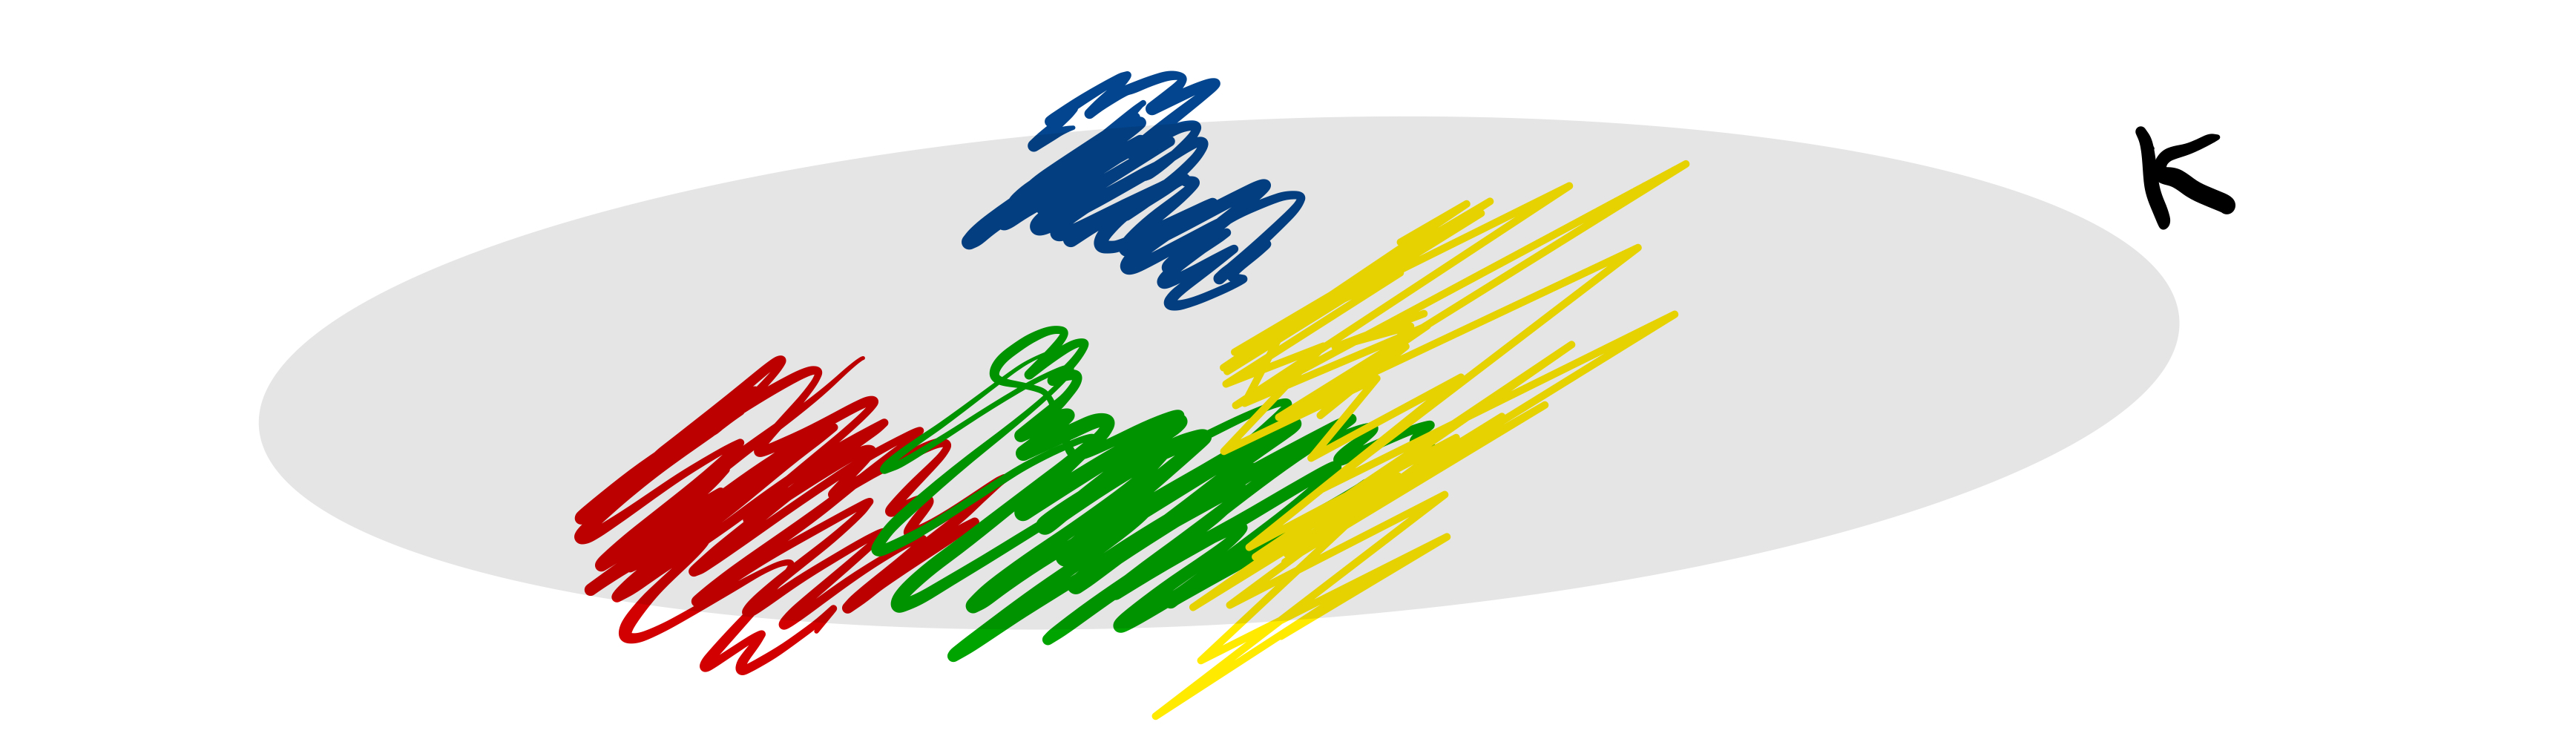
\includegraphics[scale=0.07]{tight.jpeg}
			\end{center}
			\vspace{-7mm}
			\caption*{Tightness of four measures visualised in terms of distribution of mass}
			\end{figure}
			Before we go into Prohorov's theorem let us check some examples to get some feeling of tight families.

\begin{example}
	\begin{itemize}
		\item
			By Proposition \ref{prop_4120} every family consisting of a single measure on a Polish space is tight
		\item
			$(\delta_{x_n})_{n\in\mathbb{N}}$ is a tight sequence for a Polish space $(E,d)$ if and only if $(x_n)_{n\in\N}$ is totally bounded in $E$. For instance if $(x_n)_{n\in\N}$ is bounded for $E=\R$.
		\item
			If a family $(X_\alpha)_{\alpha\in I}$ of real-valued random variables is bounded in $L^1$, then the family of the laws $\{ \mathbb{P}_{X_\alpha} \colon \alpha\in I \}$ is tight. This follows from our beloved Markov inequality as follows. If $C$ is the $L^1$-bound and $\varepsilon>0$, then $K:=[-C/\varepsilon, C/\varepsilon]$ does the job:
			\begin{align*}
				\mathbb{P}_{X_\alpha}(K^c)
				= \mathbb{P}\big(\lvert X_\alpha \rvert > C/\varepsilon\big) \overset{\text{Markov}}{\leq} \frac{\E[\lvert X_\alpha \rvert ]}{C/\varepsilon} \leq \varepsilon
			\end{align*}
		\item
			$\{ U([-n,n])\colon n\in \mathbb{N} \}$ is not tight in $\cM_f(\mathbb{R})$ as mass disappears towards infinity.
					\item If $K$ is a compact set and $(\mu_n)_{n\in\N}$ is a sequence in $\cM_1(E)$ with $\mu_n(K)=1$ for all $n\in\N$, then $(\mu_n)_{n\in\N}$ is tight.
	\end{itemize}
\end{example}
The final example shows that a good understanding of compact sets of $E$ can be extremely useful to understand tightness. We will return to this observation once we discuss in more detail $E=C([0,1])$ in which for instance sets of bounded H\"older continuous functions are compact.\smallskip

The importance of tightness becomes clear with Prohorov's famous theorem in combination with Proposition \ref{propkonvergenz}.
\begin{lsatz}
\begin{theorem}[Prohorov]\label{Prohorov}
	Let $(E,d)$ be a Polish metric space and $\cF \subseteq \cM_1(E)$, then
	\begin{align*}
		 \cF \text{ is weakly relatively sequentially compact}\quad \Leftrightarrow \quad \cF \text{ is tight}.
	\end{align*}
\end{theorem}
\end{lsatz}
The formulation of Prohorov's theorem is frightening on first sight, weakly relatively sequentially compact means that the subset $\cF$ of $\mathcal M_1(E)$ is relatively compact (the closure is compact) with respect to the topology induced by the Prohorov metric. Using properties of closures and the sequential compactness this means that every sequence $(\mu_n)$ in $\cF$ has a subsequence that converges to some limit in $\cM_f$ but the limit does not necessarily belong to $\cF$. The entire point is that Prohorov's theroem connects a measure property (tightness) with a topological property (compactness).
\begin{proof}[Proof]
	There is a relatively simple and a very hard direction. We start with the simpler one and discuss the hard direction only for $E=\R$. A sketch for the general case is given after the proof.\\
	
	"{}$\Leftarrow$": We start with arguments similar to the ones from the proof of Proposition \ref{prop_4120}. Let $x_1,x_2,...$ be dense in $E$ and 
	\begin{align*}
		A_{N,n} \coloneqq \bigcup_{k=1}^N B_{\frac{1}{n}}(x_k) \:\: \uparrow E,\quad N\to\infty.
	\end{align*}
	We first prove that
	\begin{align}\label{eq_4_1}
		\lim\limits_{N\to\infty} \inf\limits_{\mu\in\cF} \mu (A_{n,N}) =1, \quad \forall n\in\mathbb{N}.
	\end{align}
	Suppose \eqref{eq_4_1} does not hold for some $n\in\N$. Then there is some $c<1$, an increasing sequence $(N_j)$ of natural numbers and a sequence of measures $\mu_j \in \cF$ with $$\lim_{j\to\infty} \mu_j (A_{n,N_j}) \leq c < 1.$$ Since the sequence is weakly relative sequentially compact there is a subsequence $(\mu_{j_k})$ that converges to some $\mu \in \cM_1(E)$ (not necessarily in $\cF$, $\mu$ could be in $\bar{\cF}$). Since the $A_{n,N}$ are open, Portemanteau gives for all $N$
	\begin{align*}
		\mu(A_{n,N}) \leq \limsup_{k\to\infty}\mu_{j_k}(A_{n,N}) 
			\overset{\text{mon.}}{\leq} \limsup_{k\to\infty} \mu_{j_k}(A_{n,N_{j_k}}) 
			\leq c < 1.
	\end{align*}
	But this gives a contradiction: $1 = \mu(E) \overset{\text{cont.}}{=} \lim_{k\to\infty} \mu (A_{n,N_{j_k}}) \leq c<1$. \smallskip
	
	Now we use \eqref{eq_4_1} to deduce the tightness. There are $N,n_N$ with $\mu(A_{n_N,N}) \geq 1 - \frac{\varepsilon}{2^N}$ for all $\mu \in \cF$. Defining $K \coloneqq \bigcap_{N=1}^{\infty} \bar{A}_{n_N,N}$, $K$ is closed and totally bounded, hence, $K$ is compact as $E$ is complete. Additionally,
	\begin{align*}
		\mu(K^c) &= \mu \Big( \bigcup_{N=1}^{\infty} \bar{A}_{n_N,N}^c \Big) \\
			\overset{\text{sub. add.}}&{\leq} \sum_{N=1}^{\infty} \mu ( \bar{A}_{n_N,N}^c) \\
			&= \sum_{N=1}^{\infty} \big( 1 - \mu (\bar{A}_{n_N,N}) \big) \\
			\overset{\text{mon.}}&{\leq} \sum_{N=1}^{\infty} \big( 1 - \mu (A_{n_N,N}) \big) \leq \varepsilon
	\end{align*}
	for all $\mu \in \cF$. Hence, $\cF$ is tight.\smallskip
	
	"{}$\Rightarrow$": Considering only $E=\R$ we have the big advantage that one can argue using the cumulative distribution function since $$ \mu_n \overset{\text{(w)}}{\longrightarrow}\mu, \: n \to \infty \quad \Leftrightarrow \quad F_{\mu_n}(t) \to F_{\mu}(t), \: n\to\infty$$ for all points of continuity of $F$. Recall Theorem \ref{459} and keep in mind that convergence in distribution of a sequence of random variables $X_n\sim F_n$ is equivalent to weak convergence of the corresponding sequence of probability measures $\P_{F_n}$. Here we use the measures $\mu_n$ and denote the corresponding CDFs by $F_n \coloneqq \mu_n\big( ( -\infty,t]\big)$, $t\in \mathbb{R}$. Reformulated this way, Prohorov's theorem is only a theorem on CDFs: Every tight sequence of probability measures has a subsequence for which the CDFs converge to a limiting CDF at all points of continuity.\smallskip
	
	Let $(\mu_n)_{n\in\mathbb{N}}$ be a sequence in $\cF$ and $(F_n)_{n\in \mathbb{N}}$ the corresponding sequence of CDFs. Since $\big( F_n(t)\big)_{n\in\mathbb{N}}$ is bounded for all $t\in\R$ there is a convergent subsequence. Using diagonalisation \footnote{explain} there is a subsequence $(n_k)_{k\in\mathbb{N}}$ so that $F_{n_k}(q) \to \tilde{F}(q)$, $q\in\mathbb{Q}$, for some function $\tilde{F}$. We will check that
	\begin{enumerate}[label=(\roman*)]
		\item
			$F(t) \coloneqq \inf \big\{ \tilde{F}(q) \colon q > t, \: q\in \mathbb{Q}\big\}$, $t\in\R$, is a cumulative distribution function.
		\item
			$\mu_n \overset{\text{(w)}}{\longrightarrow} \mu,\,n\to\infty$, where $\mu\sim F$.
	\end{enumerate}
	Both claims are mostly technical and not too surprising, the interesting point is how the tightness comes in. The tightness is needed to prove that $F$ does not loose mass at infinity, i.e. $\lim_{t\to+\infty} F(t)=1$.
	\begin{enumerate}[label=(\roman*)]
		\item Let us check the defining properties of a cumulative distribution function. We are a bit sloppy for the claims that obviously hold even though writing the details is a bit tedious (playing with $\varepsilon$-$N$ and the definition of the infimum), those details do not lead to any deeper understanding. We actually skipped the same arguments before in the proof of Theorem \ref{kernel}.
			\begin{itemize}
				\item $F\colon \:\mathbb{R} \to [0,1]$, since $F_n \colon \mathbb{R}\to [0,1]$.
				\item $\tilde{F}$ is increasing on $\mathbb{Q}$ as all $F_n$ are increasing, then $F$ inherits the property construction.
				\item $F$ is right-continuous by definition (here one should work careful with the definition of the infimum).
				\item $\lim_{t\to+\infty}F(t) = 1$, $\lim_{t \to-\infty}F(t) = 0$ is the interesting part. This is tightness, no mass gets lost. The implications look complicated but the argument is simple:
					\begin{align*}
						\text{Tightness } \quad 
						&\Rightarrow\quad \forall \varepsilon > 0 \,\exists M\in \Q\colon \mu \big( [ -M,+M]^c \big) < \varepsilon \:\: \forall \mu \in \cF \\
						&\Rightarrow\quad \forall \varepsilon > 0 \,\exists M\in \Q\colon \mu_n \big( [ -M,+M]^c \big) < \varepsilon \:\: \forall n\in\N\\
									&\Rightarrow\quad \forall \varepsilon > 0\, \exists M\in \Q\colon 1-F_n(M)+F_n(-M) < \varepsilon \:\: \forall n \in \mathbb{N} \\
												&\Rightarrow\quad \forall \varepsilon > 0 \,\exists M\in\Q \colon F_n(M) \geq 1- \varepsilon, F_n(-M)\leq \varepsilon \:\: \forall n \in \mathbb{N} \\
												&\Rightarrow\quad \forall \varepsilon > 0 \,\exists M\in \Q\colon F(M) \geq 1- \varepsilon, F(-M)\leq \varepsilon \\
												&\Rightarrow\quad \lim_{t\to+\infty} F(t) = 1, \lim_{t\to-\infty}F(t)=0.
					\end{align*}
			\end{itemize}
		\item As explained above we can apply Theorem \ref{459} and prove the pointwise convergence of the CDFs $F_n$ at all points of continuity of $F$. Let $t$ be a point of continuity and $\varepsilon>0$. \footnote{Bild}
			Then there are $q_i \in \mathbb{Q}$ with $q_1 < q_2 < t < q_3$ with $F(q_3) - F(q_1) < \varepsilon$. Using monotonicity we have
			\begin{align*}
				F_{n_k}(q_2) \leq F_{n_k}(t) \leq F_{n_k}(q_3),
			\end{align*}
			which gives
			\begin{align*}
				\tilde F(q_2)=\liminf F_{n_k}(q_2) \leq \liminf F_{n_k}(t) \leq \limsup F_{n_k}(t) \leq \limsup F_{n_k}(q_3)=\tilde F(q_3)
			\end{align*}
			using the convergence on $\Q$. Hence,
			\begin{align*}
				F(q_1) \leq \tilde{F}(q_2) \leq \liminf F_{n_k}(t) \leq \limsup F_{n_k}(t) \leq \tilde{F}(q_3) \leq F(q_3).
			\end{align*}
			But this implies that 
			\begin{align*}
				 \liminf F_{n_k}(t),  \limsup F_{n_k}(t)\in [F(t)-\varepsilon, F(t)+\varepsilon].
			\end{align*}
			Since $\varepsilon$ is arbitrary we proved that $\lim F_{n_k}(t)$ exists and is equal to $F(x)$. 
	\end{enumerate}
\end{proof}
Here is a sketch on how the complicated "{}$\Rightarrow$"{} direction of Prohorov's theorem is proved for general Polish spaces:
\begin{enumerate}[label=(\roman*)]
	\item
		Since $E$ is separable there is a countable base $\cU \subseteq \tau$ for the topology, i.e. $O = \bigcup\limits_{U\in\cU, U \subseteq O} U$ for all $O$ open.
	\item
		Define a possible limit measure on $\cU\colon$ $\big( \mu_n(U)\big)_{n\in\mathbb{N}}$ is a bounded sequence, hence, has a converging subsequence. Since there are countably many $U_1$, $U_2$,$....\in\cU$ the same diagonalisation argument gives a subsequence such that $\big( \mu_{n_k}(U) \big)_{k\in\mathbb{N}}$ converges for all $U$.
	\item
		Define $\mu(U) \coloneqq \lim_{k\to\infty} \mu_{n_k}(U)$ for all $U \in \cU$.
	\item
		Main step: Carath\'{e}odory extension style construction of a probability measure $\bar{\mu}$ on $\cB(E)$ with $\bar{\mu}(U) = \mu(U)$ for all $U\in \cU$.
	\item
		Show $\bar{\mu}(O) \leq \liminf_{k\to\infty} \mu_{n_k}(O)$ for all $O$ open.
	\item Portemanteau implies $\mu_{n_k} \overset{\text{(w)}}{\longrightarrow} \mu$, $k\to\infty$.
\end{enumerate}
Hence, there is a weakly converging subsequence (not necessarily to a limit in $\mathcal F$) and this is precisely the relative compactness with respect to weak convergence.\smallskip

A first simple consequence of Prohorov's characterisation is the following reformulation of Proposition \ref{propkonvergenz} for weak convergence of probability measures:
\begin{lsatz}
\begin{prop}[A useful characterization of weak convergence]\label{most_useful_characterization_weak_convergence}
	Let $(E,d)$ be a Polish metric space and $\mu,\mu_1$, $\mu_2$,$...\in \cM_1(E)$. Then weak convergence of $\mu_n$ to $\mu$ is equivalent to
	\begin{enumerate}[label=(\roman*)]
			\item $\{\mu_n:n\in\N\}$ is tight,
			\item $ \lim_{n\to\infty} \int_E f \dint \mu_n = \int_E f \dint \mu$ for \underline{some} separating family $C \subseteq C_b(E)$ of $\cM_1(E)$.
		\end{enumerate}
\end{prop}
\end{lsatz}
\begin{proof}[Proof]
	"{}$\Rightarrow$": Converging sequences are relatively compact sets (in metric spaces all subsequences have the same limit), hence, tight by Prohorov's theorem. The convergence of the integrals holds by definition of weak convergence (even for all $f\in C_b(E)$).\smallskip	
	
	
	"{}$\Leftarrow$": We use Proposition \ref{propkonvergenz}. Tightness implies the sequential relative compacteness and we only need to identify $\mu$ as limit of all converging subsequences. If $(\mu_{n_k})$ is a subsequences of $(\mu_n)$ with limit $\nu$, then
\begin{align*}
	\int_E f \dint \mu=\lim_{n\to\infty} \int_E f \dint \mu_{n}=\lim_{k\to\infty} \int_E f \dint \mu_{n_k'}=\int_E f \dint \nu,\quad f\in C.
\end{align*}
The first equality holds for all $f\in C$ by assumption, the second as $(\mu_{n_k})$ is a subsequence, and the third even for all $f\in C_b(E)$. Since $C$ was assumed to be separating we proved $\nu=\mu$. 
%
%	
%	
%	Let's assume that $\mu_n$ does not converge weakly towards $\mu$. Then there is some $h\in C_b(E)$ with $$ \int_E h \dint \mu_n \not\to \int_E h \dint \mu,\quad n \to \infty$$
%	Then there is some $\varepsilon > 0$ and a subsequence $(n_k)_{k\in\mathbb{N}}$ with 
%	\begin{align}\label{eq_4_2}
%		\bigg\lvert \int_E h \dint \mu_{n_k} - \int_E h \dint \mu \bigg\rvert > \varepsilon,\quad \forall k \in \mathbb{N}.
%	\end{align}
%	Since $(\mu_{n_k})_{k\in\mathbb{N}}$ is also tight, by Prohorov's theorem there is a subsequence $(n_{k^{\prime}})_{k\in\mathbb{N}}$ of $(n_k)_{k\in\mathbb{N}}$ and a measure $\nu\in \cM_1(E)$ with $\mu_{n_{k^{\prime}}} \overset{\text{(w)}}{\longrightarrow} \nu$, hence, $$\int_E h \dint \mu_{n_{k^{\prime}}} \to \int_E h \dint \nu.$$
%	Since \eqref{eq_4_2} also holds for the subsequence we get $\int_E h \dint \mu \neq \int_E h \dint \nu$. On the other hand, by assumption, for all $f\in C_b(E)$,
%	\begin{align*}
%		\int_E f \dint \mu \overset{\mu_{n_{k^{\prime}}} \overset{\text{(w)}}{\longrightarrow} \mu}{=}\lim_{n\to\infty} \int_E f \dint \mu_{n_{k^{\prime}}} \overset{\mu_{n_{k^{\prime}}} \overset{\text{(w)}}{\longrightarrow} \nu}{=} \int_E f \dint \nu
%	\end{align*}
%	which implies $\mu = \nu$ since $C$ is a separating family. 
\end{proof}
%The next sections will deal with the prime examples that are needed for applications in probability: $(\R,|\cdot |)$ and $(\R^d,|\cdot |)$ for real-valued random variables and random vectors, $( C( [ 0, 1 ] \big), ||\cdot ||_\infty)$  and $( C( [ 0, \infty ) \big), ||\cdot ||_\infty)$ for stochastic processes.

In order to prove weak convergence we will often refer to Proposition \ref{most_useful_characterization_weak_convergence}, but there are two drawbacks that depend crucially on the underlying space $E$. One needs a good understanding of tightness (i.e. of compact sets of $E$) and one needs a good separating family. For instance for $E=C([0,1])$ it will turn out to be more useful to circumvent the formulation of Proposition \ref{most_useful_characterization_weak_convergence} and argue a bit more directly.

% !TeX spellcheck = en_US
%\chapter{Characteristic Functions and the Central Limit Theorem}
	\marginpar{\textcolor{red}{Lecture 14}}
\section[Identification of probability laws on $\R$]{Identification of probability laws on $\R^d$}\label{sec:unique}
The previous section showed how to reformulate relative sequential compactness in terms of tightness. In this section we will deal more closely with the second property from Proposition \ref{propkonvergenz}, the identification of limits of converging subsequences. We will give precise examples that help to apply Proposition \ref{most_useful_characterization_weak_convergence} for particularly simple $E$. As a side product we derive ways of determining the law of a random variable through "{}enough"{} expectations. Before doing so let us dive a bit into approximation theory.
\begin{lsatzwichtig}
\begin{theorem}[Weierstra\ss{} approximation theorem]\label{Weierstrass_approx}
	Let $f \colon [0,1] \to \mathbb{R}$ be continuous, then there is a sequence $(f_n)_{n\in\mathbb{N}}$ of polynomials on $[0,1]$ with $\left\Vert f_n - f \right\Vert_{\infty} \to 0, \: n \to \infty$.\smallskip
	
	In words: The polynomials are dense in $( C([0,1]),||\cdot||_\infty)$.
\end{theorem}
\end{lsatzwichtig}
The proof we give is awesome, as it is a probabilistic proof for an analytic theorem. The sequence of polynomials is actually given explicitly, the so-called Bernstein polynomials.
\begin{proof}[Proof]
	Let $X_1,...,X_n$ be iid Ber$(p)$-distributed random variables, hence, $S_n = \sum_{k=1}^n X_k$ is $\text{Bin}(n,p)$-distributed. Now recall the proof of the weak law of large numbers \eqref{schwaches} - Tschebycheff and Bienaymé:
	\begin{align*}
		\mathbb{P}\Big( \Big| \frac{S_n}{n}-p \Big| > \varepsilon \Big) \leq \frac{\mathbb{V}(S_n)}{n^2 \varepsilon^2} = \frac{n\V[X_1]}{n^2 \varepsilon^2} = \frac{p(1-p)}{n \varepsilon^2}
	\end{align*}
	Next, computing the discrete expectation for $\text{Bin}(n,p)$ yields
	\begin{align*}
		\E \Big[ f \Big( \frac{S_n}{n} \Big) \Big] = \sum_{k=0}^n f \Big(\frac{k}{n}\Big){n\choose k} p^k (q-p)^{n-k} = f_n(p)
	\end{align*}
	with the so-called Bernstein polynomial
		$$f_n(x) =  \sum_{k=0}^n  f \Big(\frac{k}{n}\Big){n\choose k} x^k (1-x)^{n-k},\:\: x\in [0,1].$$
	Now fix $\varepsilon > 0$. Since $f$ is uniformly continuous ($[0,1]$ is compact) there is some $\delta>0$ with
		\begin{align*}
			\lvert x - x^{\prime} \rvert < \delta \: \Rightarrow \: \lvert f(x) - f(x^{\prime}) \rvert < \varepsilon,
		\end{align*}
		so that we can estimate 
		\begin{align*}
			\Big| f \Big( \frac{S_n}{n} \Big) - f(p) \Big| \leq \varepsilon + \mathbf 1_{\lvert \frac{S_n}{n}-p \rvert \geq \delta} 2  \left\Vert f \right\Vert_{\infty}.
		\end{align*}	
		This gives
		\begin{align*}
			\lvert f_n(p) - f(p) \rvert &= \Big| \E \Big[ f \big( \frac{S_n}{n} \big) \Big] - \E \big[ f(p) \big] \Big| \\
									&\leq \E \Big[ \Big| f \Big( \frac{S_n}{n} \Big) - f(p) \Big| \big] \\
									&= \varepsilon + 2 \cdot \left\Vert f \right\Vert_{\infty} \mathbb{P} \Big( \Big| \frac{S_n}{n}-p \Big| \geq \delta \Big) \\
									&\leq \varepsilon +  2 \cdot \left\Vert f \right\Vert_{\infty} \cdot \frac{p(1-p)}{n\cdot \delta}.
		\end{align*}
		Putting together what we have so far we obtain
		\begin{align*}
			\left\Vert f_n - f \right\Vert_{\infty} = \sup_{p \in [0,1]} \lvert f_n(p) - f(p) \rvert \leq \varepsilon +  2 \cdot \left\Vert f \right\Vert_{\infty} \cdot \frac{1}{n \delta^2} \rightarrow \varepsilon,\quad n\to \infty.
		\end{align*}
		Since $\varepsilon$ was arbitrary, we proved that $\left\Vert f_n - f \right\Vert_{\infty} \to 0$, $n \to \infty$.
\end{proof}
It turns out that classes of complex-valued functions are more useful than only real-valued functions. For that sake let us recall some definitions and facts for the complex numbers:
\begin{lstep}
  As a set the complex numbers are identical to $\R^2$ with a different notation for the vectors: $$\mathbb{C}\coloneqq \{ z = u+iv \,|\, u,v\in\mathbb{R} \}.$$ The following properties will be used:
	\begin{itemize}
		\item $\lvert z \rvert = \sqrt{u^2 + v^2}$
		\item $\mathcal{R}e(z) = u, \: \mathcal{I}m(z) = v$
		\item Seen as a metric space $( \mathbb{C}, |\cdot| )$ is a Polish metric space and identical to $(\R^2,|\cdot|)$. In particular $\mathcal B(\C)=\mathcal B(\R^2)$ and in terms of measure theory all results from Section \ref{sec:RV} apply. As an example, using Proposition \ref{zweiInterpr}, a $\C$-valued random variable $X\colon \Omega \to \mathbb{C}$ is measurable if and only if $\mathcal{R}e(X)$ and $\mathcal{I}m(X)$ are measurable.
				\item Complex conjugation: $\bar{z} = u - i \cdot v$
		\item Polar coordinates: $z = \lvert z \rvert \cdot e^{i \varphi}$ for an angle $\varphi\in [0,2\pi)$.
		\item Multiplication $z_1\cdot z_2:= (u_1u_2+u_2v_2)+i(u_1v_2+v_2u_1)$ so that $i^2=-1$, or in polar coordinates: $z_1 \cdot z_2 = \lvert z_1 \rvert \, \lvert z_2 \rvert e^{i(\varphi_1 + \varphi_2)}$, which corresponds to rotation and expanding.
		\item Addition: $z_1 + z_2 = (u_1+u_2)+i(v_1+v_2)$
		\item Field with $+,\cdot$, $0=(0,0)$, $1=(1,0)$
		\item $\mathcal{R}e(z) = \frac{z+ \bar{z}}{2},\: \mathcal{I}m(z) = \frac{z-\bar{z}}{2i}$
		\item Exponential function $\exp\colon \mathbb{C} \to \mathbb{C}$ 
			\begin{align*}
				\sum_{k=0}^{\infty} \frac{z^k}{k!}=\exp(z) = \exp(u+iv) &= \exp(u)\exp(iv)
			\end{align*}
			with
			$$\exp(z_1 + z_2) = \exp(z_1)\exp(z_2).$$
			and Euler formula
			$$\exp(iv)=\cos(u)+i \sin(v)$$
			that implies $|e^{iv}|=1$ for all $v\in\R$.
		\item $\cos(u) = \frac{e^{iu}+ e^{-iu}}{2}$, $\sin(u) =  \frac{e^{iu} - e^{-iu}}{2i}$
	\end{itemize}
\end{lstep}
	Complex integration of functions $f:\C\to\C$ is covered in complex analysis lectures with all magic tricks to compute such integrals. We will not touch upon this topic and only define the Lebesgue integral for measurable $f:\Omega\to \C$ by integrating separately real- and imaginary part:
	\begin{align*}
		\int_{\Omega} f \dint \mu := \int_{\Omega} \mathcal{R}e(f) \dint \mu + i  \int_{\Omega} \mathcal{I}m(f) \dint \mu\in \C
	\end{align*}	
	if both (real-valued) integrals exist. Rules for the integral can be deduce from rules for both (real-valued) integrals. Expectations of complex-valued random variables are defined as follows: $$\E[X]:=\int_\Omega X(\omega)\dint \P(\omega)=\int_\Omega \mathcal{R}e(X)(\omega)\dint \P(\omega)+i\int_\Omega \mathcal{I}m(X)(\omega)\dint \P(\omega)\in \C$$ which can be computed with typical tools for real-valued random variables since $$\E[X]=\E[\mathcal{R}e(X)]+i\,\E[\mathcal{I}m(X)].$$
	An important special case appears when $X$ is a real-random variable and $g:\R\to\C$. Expectations can be calculated in the usual way as
	\begin{align}\label{expec}
		\E[g(X)]=\begin{cases}
			\int_\R g(x) f(x)\dint x&: X\text{ is absolutely continuous with density }f\\
			\ \sum_{k=1}^N g(a_k)p_k&: X\text{ is discrete with values }a_k \text{ and probabilities }p_k
		\end{cases}.
	\end{align}
	To see why just split the expectations into two real-valued expectations, use the standard formulas and put them together. The most important example that we will discuss below is $\E[e^{itX}]$ for real-valued random variables.	





\begin{ldef}
\begin{deff}\label{def_separating_points}
	Let $(E,d)$ be a metric space and $K = \mathbb{R}$ or $K = \mathbb{C}$. A subset $C \subseteq C_b(E,K)$ is called an \textbf{algebra} of functions if
	\begin{itemize}
		\item $1 \in C$,
		\item $f,g\in C \: \Rightarrow \: f\cdot g, \: f+h \in C$,
		\item $f\in C, \: \alpha \in K \: \Rightarrow \: \alpha \cdot f \in C$,
	\end{itemize}
	 If $K = \mathbb{C}$ we always assume $C$ is closed under complex conjugation. We say the \textbf{algebra $C$ separates points} if for all $y,x\in E$ there is some $f\in C$ with $f(x) \neq f(y)$.
\end{deff}
\end{ldef}
There are many examples of algebras, for instance the set of polynomials or all exponential functions. We will discuss the examples in the upcoming sections but first deal with an important generalisation of the Weierstra\ss{} approximation theorem. The Stone-Weierstra\ss{} approximation theorem allows to generalise the $[0,1]$ to some compact metric space and the polynomials to any algebra of functions:
\begin{lsatzwichtig}	
\begin{theorem}[Stone-Weierstra\ss{} approximation theorem]\label{Stone_weierstrass}
	Let $(E,d)$ a compact metric space, $K = \mathbb{R}$ or $K = \mathbb{C}$, and $C \subseteq C_b(E, K ) $ an algebra of functions that separates points.
	Then $C$ is dense in $\big( C_b(E,K), ||\cdot||_\infty \big)$.
\end{theorem}
\end{lsatzwichtig}
To see why the algebra should separate points take as an example the set of all constant functions. This forms an algebra, does not separate points and is clearly not large enough to approximate all bounded continuous functions.

\begin{proof}[Proof]
Let us first consider the case $K = \mathbb{R}$.
\begin{enumerate}[label=(\roman*)]
	\item First note that also $\bar C$ is an algebra, as the defining properties rely on continuous operations that transfer through taking limits (recall that $\bar C$ consists of all limits of sequences from $C$). By the  is Weierstra\ss{} approximation theorem there is a sequence $(p_n)_{n\in \mathbb{N}}$ of polynomials with $p_n \to p,n\to \infty,$ uniformly on $[0,1]$, where $p(x) = \sqrt{x}$. If $f \in \bar{C}$, then $\lvert f \rvert \in \bar{C}$ because $$ \lvert f \rvert = \left\Vert f \right\Vert_{\infty} \cdot {\lim_{n\to\infty} \underbrace{p_n \Big( \frac{f^2}{ \underbrace{\left\Vert f \right\Vert_{\infty}^2}_{\in [0,1]}}\Big)}_{\in \bar C \text{ as }\bar{C} \text{ is an algebra}}}\in \bar C,$$
		as $\bar C$ is closed. Using $f \vee g = \frac{1}{2} ( f + g + \lvert f - g \rvert )$ and $ f \wedge g = \frac{1}{2} ( f + g - \lvert f - g \rvert )$ we see that the algebra $\bar{C}$ (operations transfer to limit) is also closed under taking pointwise maxima and minima.
	\item
		Now fix $\varepsilon>0$. Let $f \in C_b(E, \mathbb{R})$ and $x \in E$. Then there is $g_x \in \bar{C}$ with 
		\begin{itemize}
			\item $g_x(x) = f(x)$,
			\item $g_x(y) \leq f(y) + \varepsilon$, $\forall y \in E$.
		\end{itemize}
		To see why note that $C$ separates points, hence, for all $z \in E \setminus \{x \}$ there is a function $H_z \in C$ with $H_z(z) \neq H_z(x).$ By adding a constant we can assume that $H_z(x)=0$. Next, define $h_x=f$ and, for $z\neq x$,
		\begin{align*}
			h_z(y) := 
				 f(z) + \frac{f(x)-f(z)}{H_z(x)}\cdot H_z(y),\quad y\in E,
		\end{align*}
		which is a function in $C$ that coincides with $f$ in $x$ and $z$.
		Since $f$ and $h_z$ are continuous, for all $z \in E$ there is a neighbourhood $U_z $ of $z$ with $h_z \leq f + \varepsilon$ on $U_z$. Using compactness there is a finite covering $U_{z_1},..., U_{z_n}$ of $E$ of such neighbourhoods. If finally we define $g_x \coloneqq \min \{h_{z_1},...,h_{z_n} \}$, then $g\in \bar C$ by (i) and $g$ satisfies the two claimed properties by the construction.
	\item
		Since $f$ and $g_x$ are continuous and $f(x) = g_x(x)$ there are neighborhoods $U_x$ of $x$ with $g_x \geq f - \varepsilon$ on $V_x$. By compactness finitely many $V_{x_1},...,V_{x_k}$ cover $E$. Then define $g \coloneqq \max \{ g_{x_1},...,g_{x_k} \} \in \bar{C}$. By construction this gives $f + \varepsilon \geq g \geq f - \varepsilon$ or $\left\Vert f - g \right\Vert_{\infty} < \varepsilon$. Since $\varepsilon$ is arbitrary we can find a sequence in $\bar C$ that converges uniformly to $f$. In other words, $\bar{C} = C_b(E, \mathbb{R})$.
\end{enumerate}
It remains to consider the case $K = \mathbb{C}$. If $f =\mathcal{R}e(f)+\mathcal{I}m(f) \in C$, then real- and imaginary-part are in $C$. This follows from the assumption on $C$ by writing $\mathcal{R}e(f) = \frac{f + \bar{f}}{i}$ and $\mathcal{I}m(f) = \frac{f - \bar{f}}{2i}$. Hence, 
\begin{align*}
	C_{\mathcal{R}}:=\{ \mathcal{R}e(f) \colon f \in C \}\subseteq C\quad \text{and}\quad 	C_{\mathcal{I}}:=\{ \mathcal{I}m(f) \colon f \in C \} \subseteq C
\end{align*}	
	and, thus, both form algebras of real functions. Both sets are also separating according to the following trick. Suppose $x$ and $y$ are separated by $f\in C$, that is $f(x)\neq f(y)$. Since $C$ is closed under adding $1$ and multiplication with constants (which is rotation and stretching) there are functions $h, g\in C$ such that
	\begin{align*}
		h(x)=ia_1,\, h(y)=a_2+ia_3\quad \text{and}\quad g(x)=b_1+ib_2, \,g(y)=b_3
	\end{align*}
	for some $a_i,b_i\neq 0$.
	Thus, $$\mathcal{R}e(h)(x)=0\neq b_1= \mathcal{R}e(g)(x)\quad \text{and}\quad \mathcal{I}m(h)(y)=a_3\neq 0= \mathcal{I}m(g)(y).$$ Hence, $\mathcal{R}e(h)\in C_{\mathcal{R}}$ and $\mathcal{I}m(g)\in C_{\mathcal{I}}$ both separate $x$ and $y$.
	This proves that $C_{\mathcal R}$ and $C_{\mathcal I}$ are separating algebras of real functions. Why did we need to involve this little trick? It is possible that the imaginary parts and/or real parts of $f(x)$ and $f(y)$ coincide. If they do, then the imaginary parts and/or real parts of $f$ do not separate $x$ and $y$. To avoid this problem we can multiply $f$ by a constant $z'$ to rotate (and stretch) the complex numbers $f(x)$ and $f(y)$ to ensure that the real and imaginary parts of $h(z):=z'f(z)\in C$ differ and thus separate points. The trick is best understood in a picture:
	\begin{figure}[h]
		\vspace{-3mm}
		\begin{center}
			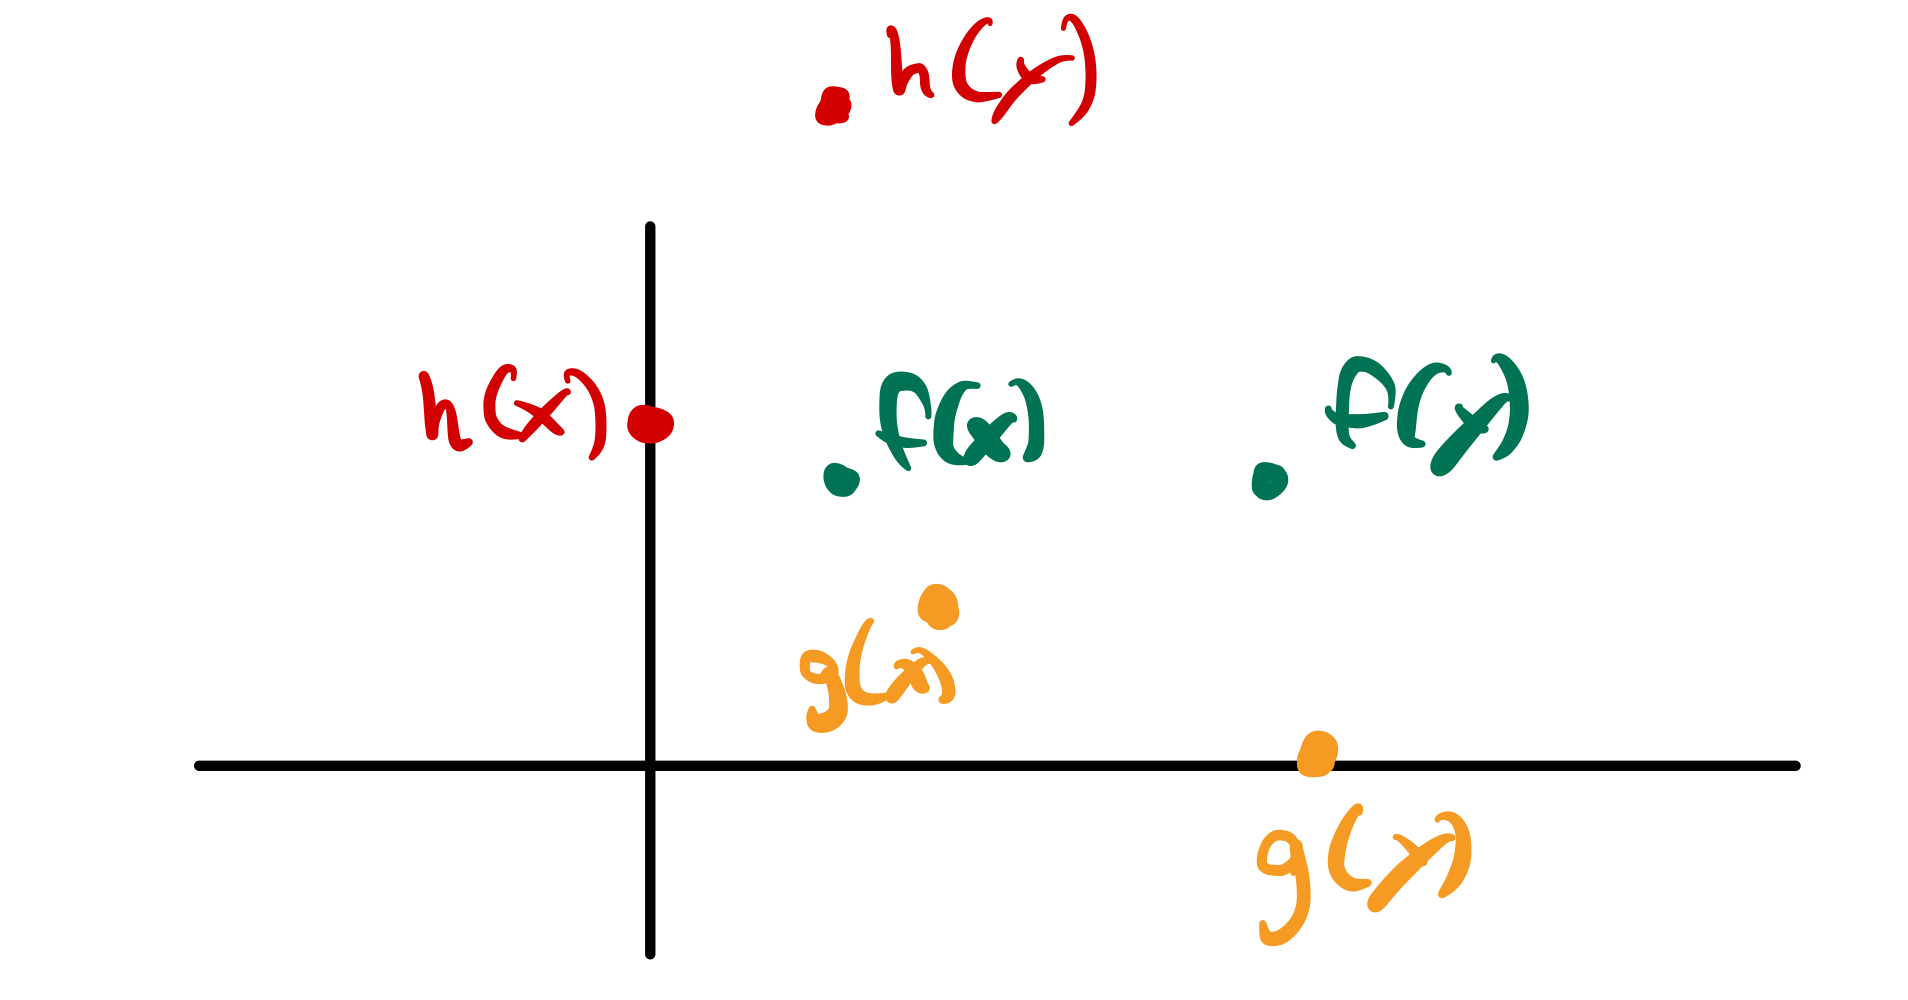
\includegraphics[scale=0.07]{complex.jpeg}
		\end{center}
		\vspace{-3mm}
		\caption*{The rotation trick to separate points}
		\end{figure}	

	Therefore, from the above, $\bar{C}_{\mathcal R} = \bar{C}_{\mathcal I} = C_b(E,\mathbb{R})$. Since $C_b(E, \mathbb{C}) = C_b(E,\mathbb{R}) + i \cdot C_b(E,\mathbb{R})$ we find that $C = C_{\mathcal{R}} + i \cdot C_{\mathcal{I}}$ is dense in $C_b(E, \mathbb{C})$.
\end{proof}
What is the magic of Stone-Weierstra\ss? Proving that families of functions are dense in other families is typically hard, a purely analytic $\varepsilon$-$N$ story. Stone-Weierstra\ss{} allows us to prove the density in a completely different way, only checking very simple algebraic properties! If we think about polynomials or exponential functions the algebraic properties are easily checked.\smallskip
\marginpar{\textcolor{red}{Lecture 15}}

The situation becomes even simpler if integrals are involved as linearity of integrals fits nicely to the properties of algebras.
\begin{llemma}
\begin{corollary}\label{cor_514}
	Let $(E,d)$ be a compact metric space and $C \subseteq C_b(E,K)$ a family that separates points, is closed under multiplication and contains $1$ (constant $1$ function). Then $C$ is separating for $\cM_1(E)$.
\end{corollary}
\end{llemma}
The examples that will appear in the sequal are typically polynomials or exponential functions on compact subsets of $\R$.
\begin{proof}[Proof]
	We start with a little trick on separating functions and algebras that relies on the linearity of integrals. Let $\mu,\: \nu \in \cM_1(E)$ with $\int_E g \dint \mu = \int_E g \dint \mu$ for all $g \in C$. Taking all linear combinations of functions in $C$ and calling them $C'$ then by linearity of integrals the equality also holds for all functions in $C'$ and $C'$ is an algebra of functions. Using the Stone-Weierstra\ss{} theorem, the equality of integrals holds for a dense subset of $C_b(E)$.
	\smallskip
	
	Fix $\varepsilon>0$. Then for all $f \in C_b(E)$ there exists $g \in C^{\prime}$ with $\left\Vert f - g \right\Vert_{\infty} < \varepsilon$ so that 
	\begin{align*}
		&\quad\Big| \int_E f \dint  \mu - \int_E f \dint \nu \Big|  \\ 
		&\leq \Big| \int_E f \dint \mu - \int_E g \dint \nu \Big| + \Big| \int_E g \dint \nu - \int_E g \dint \mu \Big| + \Big| \int_E g \dint \mu - \int_E f \dint \nu \Big| \\
		&\leq \left\Vert f - g \right\Vert_{\infty} \cdot \mu(E) + 0 + \left\Vert f - g \right\Vert_{\infty} \cdot \nu(E) = 2 \varepsilon.
	\end{align*}
	Since this works for all $\varepsilon > 0$ it follows that $$\int_E f \dint \mu = \int_E f \dint \nu,\quad \forall f\in C_b(E).$$ Recalling from Proposition \ref{theorem_4124} that $C_b(E)$ is separating for $\cM_1(E)$ we proved $\mu = \nu$. Hence, $C$ is separating for $\cM_1(E)$.
\end{proof}

\begin{lsuperwichtigersatz}
\begin{theorem}\label{coruniq}
	\begin{enumerate}[label=(\roman*)]
		\item Every measures $\mu\in \mathcal M_1([a,b])$ is uniquely determined by all integrals $$\int_{[a,b]} x^m \dint \mu(x),\quad m\in\N_0.$$
		\item The law of a \underline{bounded} real-valued random variable is determined by all it's moments, i.e. if $\E[X^m]=\E[Y^m]$ for all $m\in\N$, then $X\sim Y$.

	\end{enumerate}
\end{theorem}
\end{lsuperwichtigersatz}
\begin{proof}[Proof] All we need to do is to apply Corollary \ref{cor_514}.\smallskip

First note that $([a,b],|\cdot|)$ is a compact metric space. Define $C$ to be the family of monomials on $[a,b]$, that is $C = \{ x^m \colon m \in \mathbb{N}_0 \}$. Then $C$ is closed under multiplication, separates points in $[a,b]$ and contains the constant $1$ function. Hence, $C$ is a separating family for $\cM_1([a,b])$. But then, recalling the definition of a separating family,
\begin{align*}
	\int_{[a,b]} x^m \dint \mu(x)=\int_{[a,b]} x^m \dint \nu(x),\quad \forall m\in\N_0,
\end{align*}
implies $\nu=\mu$.\smallskip

The second claim follows from the first claim applied to the laws $\P_X$.
\end{proof}





\begin{lsuperwichtigersatz}
\begin{theorem}\label{cor_distributions_1}
	\begin{enumerate}[label=(\roman*)]
		\item Every measures $\mu \in \mathcal M_1([0,\infty)])$ is uniquely determined by all integrals $$\int_{[0,\infty)} e^{-\lambda x}\dint \mu(x),\quad \lambda>0.$$
		\item The law of a \underline{\smash{non-negative}} random variable is determined by it's Laplace transformation $L_X(\lambda) \coloneqq \E \big[ e^{- \lambda X} \big]$, $\lambda \geq 0$, i.e. if $L_X=L_Y$ then $X\sim Y$.
	\end{enumerate}
\end{theorem}
\end{lsuperwichtigersatz}
Of course part (ii) of the theorem also holds for non-positive random variables replacing the Laplace transformation by the moment generating function $M_X(t)=\E[e^{tX}]$ for all $t>0$.
\begin{proof}[Proof]
As in the previous proof we would like to apply Corollary \ref{cor_514} to the family of exponential functions, but there is a problem as $[0,\infty)$ is not compact. We apply a trick from Functional Analysis and use $E = [0, \infty]$ instead (the so-called one-point compactification).
\begin{luebung}
	$([0,\infty],d)$ is a compact metric space with $d(x,y):=|e^{-x}-e^{-y}|$. The metric is compatible with the usual convergence in $[0,\infty]$.
\end{luebung}
Note that convergence towards $\infty$ is divergence from basic analysis. Continuity of functions $f:[0,\infty]\to \R$ is best understood through sequences, $\lim_{n\to\infty} f(x_n)=f(x)$ and this takes in particular sequences that diverge to $\infty$. Hence, we can extend continuous functions on $[0,\infty)$ to continuous functions on $[0,\infty]$ if and only if $\lim_{x\to\infty} f(x)$ exists and in that case we must set $f(\infty)=\lim_{x\to\infty} f(x)$. For the exponential functions we thus define
\begin{align*}
	f_{\lambda}(x) \coloneqq \begin{cases}
			e^{- \lambda x} &: x>0 \\
			0 &: x = \infty, \lambda>0\\
			1 &: x = \infty, \lambda=0
			 \end{cases}.
\end{align*}
Then $C\coloneqq \{ f_{\lambda} \colon \lambda > 0 \}\subseteq C_b([0,\infty])$ separates points, $f_0 \equiv 1\in C$, and $f_{\mu}\cdot f_{\lambda} = f_{\mu + \lambda}$. Hence, $C$ separates probability measures on $\cB([0,\infty])$ and in particular measures on $\cB([0,\infty))$ which can be extended to $\cB([0,\infty])$ by extending a measure $\mu$ with $\bar{\mu}(\{ +\infty \} ) = 0$. That is, for $\nu, \mu\in \cM([0,\infty])$,
\begin{align*}
	&\quad \int_{[0,\infty)} e^{-\lambda x}\dint \mu(x)
	=\int_{[0,\infty)} e^{-\lambda x}\dint \nu(x),\quad \forall \lambda \geq 0\\
	& \Rightarrow \quad \int_{[0,\infty]}f \dint \bar \mu=\int_{[0,\infty]}f \dint \bar \nu,\quad \forall f\in C\\
	& \Rightarrow\quad \bar \mu=\bar \nu\\
	& \Rightarrow\quad \mu=\nu.
\end{align*}	
The second claim follows from the first claim applied to the laws $\P_X$.
	%	Let us assume $X$ and $Y$ take values in $[0,1]$, otherwise both are multiplied by the same constant which equally changes the moments. Now define $C$ to be the family of monomials, that is $C = \{ f_n \colon n \in \mathbb{N}_0 \}$ where $f_n=x^n$. Then $C$ is closed under multiplication, separates points in $[0,1]$ and contains the constant $1$ function. Hence, $C$ is a separating family for $\cM_1([0,1])$. But then, recalling the definition of a separating family,
%	\begin{align*}
%		\int_{[0,1]} f_n \dint \P_X= \E[X^n]  = \E[Y^n]= \int_{[0,1]} f_n \dint \mathbb{P}_Y,\quad \forall n \in \mathbb{N},
%	\end{align*}
%	implies $\mathbb{P}_X = \mathbb{P}_Y$, which is $X \sim Y$.
\end{proof}
Could we extend the same argument also to all measures on $\R$ (i.e. all random variables)? No! To do so we needed a family that is closed under multiplication (that leads to polynomials or exponentials) that converge at $+\infty$ and $-\infty$. Trying to find such a family is a good exercise to better understand the previous proofs. The trick that we get to know below is to replace the exponential functions by complex exponential functions.\smallskip

\begin{luebung}
	A little induction shows that all moments of $U\sim \mathcal U([a,b])$ are given by 
	\begin{align}\label{momuniform}
		\E[U^n]=\frac{1}{n+1}\sum_{k=0}^na^kb^{n-k}=\frac{b^{n+1}-a^{n+1}}{(n+1)(b-a)}	
	\end{align}
\end{luebung}
If for some reason one can show that a random variable has the moments from \eqref{B55}, then the random variable must be uniform. \smallskip

It is important to have an example in mind that shows that all moments do not uniquely determine the law of unbounded random variables. Here is nice counterexample that appears in the Black-Scholes theory of time-continuous financial markets. A random variable $X$ is called \textbf{log-normal} distributed if $X = \exp(Z)$, with $Z \sim \cN(0,1)$. Using substitution in $\P(X\leq t)=\P(Z\leq \log(t))=\int_{-\infty}^{\log(t)} \frac{1}{\sqrt{2\pi}} e^{-\frac{x^2}{2}}\dint x$ shows that $X$ has density $$ f_X(x) = \frac{1}{\sqrt{2 \pi}} \frac{1}{x} e^{- \frac{1}{2} \log(x)^2}\mathbf 1_{[0,\infty)}(x),\quad x\in\R.$$ From the moment generating function of the standard Gaussian distribution (see \ref{momg}) we obtain a formula for the moments: $\mathbf E\big[X^n \big] = \mathbf E \big[ e^{n\cdot Z} \big] = e^{\frac{1}{2}n^2}$. Next, we will write down an entire family of density functions that give the same moments but are log-normal densities. For $\alpha \in [-1,1]$ define
\begin{align*}
	f_{\alpha}(x) \coloneqq f_X(x) \cdot \big( 1 + \alpha \cdot \sin(2 \pi \log(x) \big)\mathbf 1_{[0,\infty)}(x),\quad x\in\R.
\end{align*}
Those functions are clearly non-negative and the computation below for $n=0$ shows they integrate to $1$, hence, they are densities. To prove the moments are identical to those of the log-normal distribution it suffices to show that 
\begin{align*}
	m(n) := \int_0^{\infty} x^n \cdot f_X(x) \cdot \sin(2 \pi \log(x)) \dint x = 0,\quad \forall n \in \mathbb{N}_0,
\end{align*}
and combine with $\int_\R x^n\cdot f_X(x)\dint x=\E[X^n]=e^{\frac{1}{2}n^2}$. Here is the computation:
\begin{align*}
	m(n) &= \int_{-\infty}^{\infty} e^{y\cdot n} \cdot f_X( e^y) \cdot \sin(2 \pi y ) \cdot e^y \dint y \\
		\overset{\text{subst. }y=z+n}&{=} \int_{-\infty}^{\infty} e^{zn + n^2} f_X(e^{z+n}) \sin(2 \pi z + 2 \pi n) e^{z+n} \dint z \\
		&= \frac{1}{\sqrt{2\pi}} e^{n^2} \int_{-\infty}^{\infty} e^{-\frac{1}{2}z^2-\frac{1}{2}n^2} \sin(2 \pi z) \dint z \\
		&= \frac{1}{\sqrt{2 \pi}} e^{\frac{1}{2}n^2} \underbrace{\int_{-\infty}^{\infty} e^{-\frac{1}{2}z^2} \sin(2 \pi z ) \dint z}_{ = 0 \text{, odd function and integrable}}=0.
\end{align*}
That's it.\smallskip

No doubt, the most exciting random variables (such as the Gaussian) are neither concentrated on a bounded interval nor are positive (or negative). In general the law is not determined only by moments as $\R$ (or $\R^d$) cannot be compactified such that enough functions are continuous on the compactification. Hence, an approach different from the Stone-Weierstra\ss{} theory is needed.\smallskip

The alternative approach uses the periodic structure of $e^{it}$:
\begin{ldef}
\begin{deff}

			For $\mu \in \cM_1(\mathbb{R}^d)$ the function $\varphi_\mu:\R^d\to\C$ defined by $$\varphi_{\mu}(t) \coloneqq \int_{\mathbb{R}^d} e^{\langle t,x \rangle} \dint\mu (x) \quad t\in \mathbb{R}^d,$$ is called the \textbf{characteristic function} (or Fourier transform) of $\mu$.
\end{deff}
\end{ldef}
The wording Fourier transformation comes from Fourier Analysis where integrable functions are studied through their Fourier transform $\hat{f}(x) \coloneqq \int e^{i\langle x, y \rangle} f(y) \dint y$. In probability theory people prefer to use the name characteristic function as a random variable is uniquely characterised through the characteristic functions.\smallskip

As always we can either define objects for probability measures or random variables with the corresponding law. Since the characteristic function is such an important object let us fix the other notation as well:
\begin{ldef}
\begin{deff}
			For a random vector $X$ the function $\varphi_X:\R^d\to\C$ defined by $$\varphi_X(t) \coloneqq \E[e^{i \langle t, X \rangle}] = \varphi_{\mathbb{P}_X}(t), \quad t\in \mathbb{R}^d,$$ is called the textbf{characteristic function of $X$}.
\end{deff}
\end{ldef}
			 The characteristic function plays exactly the same role as moment generating function $\mathcal M_X$, or the distribution function $F_X$. It is just a function with certain properties (see below) that can be used to study more complicated mathematical objects such as measures or random variables. The major advantage of the characteristic function is that $\varphi$ is always well-defined because $\varphi_X$ is always defined as $\lvert e^{ix} \rvert = 1$.\smallskip

Here are some properties that indicate that characteristic functions are useful to work with:
\begin{llemma}
\begin{lemma}\label{lemma_5111}
	Let $X$ be a random vector and $\varphi_X \colon \mathbb{R}^d \to \mathbb{C}$ the characteristic function.
	\begin{enumerate}[label=(\roman*)]
		\item $\varphi_X(0) = 1$ and $\lvert \varphi_X(t) \rvert \leq 1$ for all $t \in \mathbb{R}^d$.
		\item $\varphi_{aX+b}(t) = \varphi_X(a t)  e^{i\langle b,t \rangle}$ for all $ a \in \mathbb{R}$ and $b\in \mathbb{R}^d$.
		\item $\varphi$ is real-valued if and only if $X$ is symmetric, i.e. $\mathbb{P}_X = \mathbb{P}_{-X}$.
		\item $\varphi_{X+Y} = \varphi_X \cdot \varphi_Y$ if $X$ and $Y$ are independent.
	\end{enumerate}
\end{lemma}
\end{llemma}
\begin{proof}[Proof]
	If you are not used to integrals for complex-valued functions the arguments are a bit more complicated than one might think.
	\begin{luebung}
		To get started please check the linearity $\int (\alpha f+\beta g)\dint \mu=\alpha \int f \dint \mu+\beta \int f \dint \mu$ for $\alpha, \beta \in\C$ of complex integrals by using the definition and properties of real integrals.
	\end{luebung}
	\begin{enumerate}[label=(\roman*)]
		\item Let us first assume the usual triangle inequality also for complex integrals. Then we obtain
			\begin{align*}
				\lvert \varphi_X(t) \rvert 
				= \big| \E \big[ e^{i \langle t,X \rangle} \big] \big| 
				= \Big| \int_{\Omega} e^{i \langle t, X(\omega) \rangle} \dint \mathbb{P}(\omega) \Big|
				\overset{\Delta}{\leq} \int_{\Omega} \big| e^{i \langle t, X(\omega) \rangle} \big| \dint \mathbb{P}(\omega)
				= \int_\Omega 1\dint \P(\omega) = 1.
			\end{align*}
			The triangle inequality $|\int_\Omega f\dint \mu|\leq \int_\Omega |f|\dint \mu$ is more complicated than one might think. Suppose $\varphi$ is the angle from the polar coordinate representation of $\int_\Omega f\dint \mu$. Then
			\begin{align*}
				\Big|\int_\Omega f \dint \mu \Big| = e^{-i\varphi} \int_\Omega f \dint \mu
				=\int_\Omega e^{-i\varphi} f \dint \mu
				=\int_\Omega \mathcal{R}e(e^{-i\varphi} f) \dint \mu
				\leq \int_\Omega |e^{-i\varphi} f| \dint \mu
				= \int_\Omega  |f| \dint \mu.
			\end{align*}
			The first equality holds as multiplying with $e^{-i\varphi}$ is a rotation, the second is linearity, the third holds as $|\cdot|\in \R$ so that the imaginary part of the integral vanishes, and the fourth is monotonicity for real-valued integrals. Finally, the fifth equality is $|e^{-i\varphi}f|=|e^{-i\varphi}||f|=|f|$.
		\item
			Write it down yourself!
		\item Recall that
			$e^{-i\theta} = \cos(-\theta) + i \sin(-\theta) = \cos(\theta) - i \sin(\theta) = \overline{e^{i \theta}}$, hence, 
			\begin{align*}
				\varphi_{-X}(t) = \E \big[ e^{-i \langle X, t \rangle} \big] = \E \big[ \overline{ e^{i \langle X, t \rangle}} \big] = \overline{\E [ e^{i \langle X, t \rangle}]} = \overline{\varphi_X(t)},
			\end{align*}
			where we used
			\begin{align*}
				\overline{\int f\dint \mu}=\overline{\int \mathcal{R}e(f)\dint \mu+i\int \mathcal{I}m(f)\dint \mu}=\int \mathcal{R}e(f)\dint \mu-i\int \mathcal{I}m(f)\dint \mu=\int \overline{f}\dint \mu.
			\end{align*}
			The claim now follows immediately.
			\item The proof is essentially the same that we have seen for moment generating functions in Proposition \ref{P7}. All we need to do is to extend Theorem \ref{un} to complex-valued functions. But this is simple using the linearity from above:
			\begin{luebung}
				Check that $\E[f(X)g(Y)]=\E[f(X)]\E[g(Y)]$ holds for independent random variables $X$ and $Y$.
			\end{luebung}
		%\begin{align*}
		%	\E[f(X)f(Y)]&=\E[\mathcal{R}e (f)(X)\mathcal{R}e (g)(X)]+i\E[\mathcal{R}e (f)(X)\mathcal{I}m (g)(X)]\\
		%	&\quad +i\E[\mathcal{I}m (f)(X)\mathcal{R}e (g)(X)]-\E[\mathcal{I}m (f)(X)\mathcal{I}m (g)(X)]\\
		%\overset{\ref{un}}&{=}\E[\mathcal{R}e (f)(X)]\E[\mathcal{R}e (g)(X)]+i\E[\mathcal{R}e (f)(X)]\E[\mathcal{I}m (g)(X)]\\
		%	&\quad +i\E[\mathcal{I}m (f)(X)]\E[\mathcal{R}e (g)(X)]-\E[\mathcal{I}m (f)(X)]\E[\mathcal{I}m (g)(X)]\\
		%	&=(\E[\mathcal{R}e (f)(X)]+\E[\mathcal{I}m (f)(X)])\cdot (\E[\mathcal{R}e (g)(X)]+\E[\mathcal{I}m (g)(X)])\\
		%	&=\E[f(X)]\cdot \E[g(Y)].
		%\end{align*}
		But then 
		\begin{align*}
			\varphi_{X+Y}(t)=\E[e^{i\langle t,X+Y\rangle}]=\E[e^{i\langle t,X\rangle}]\cdot \E[e^{i\langle t,Y\rangle}]=\varphi_X(t)\cdot \varphi_Y(t),
		\end{align*}
		for all $t\in\R$.
	\end{enumerate}
\end{proof}
	\marginpar{\textcolor{red}{Lecture 16}}

	To get a feeling let us check some examples.
	\begin{example}
		Using the discrete computation rule from \eqref{expec} yields
		$$\varphi_{\text{Poi}(\lambda)}(t) = \E \big[ e^{itX} \big] = \sum_{k=0}^{\infty} e^{-\lambda} e^{itk} \frac{\lambda^k}{k!} = e^{\lambda (e^{it}-1)}e^{\lambda ( e^{it} - 1)},\quad t\in\R,$$
		and
		\begin{align*}
			\varphi_{\text{Bin}(n,p)}(t)
			&=\E\big[ e^{itX} \big]\\
			&= \sum\limits_{k=0}^{n} {n\choose k} e^{itk}p^k (1-p)^{n-k}\\
			&= \sum\limits_{k=0}^{n}{n\choose k} (p  e^{it})^k (1-p)^{n-k} = \big( 1 - p +p  e^{it} \big)^n,\quad t\in\R.
		\end{align*}
		The second example can also be computed from (iv) of Lemma \ref{lemma_5111} using
		\begin{align*}
			\varphi_{\text{Ber}(p)}(t)=\E[e^{itX}]=e^{it}p+(1-p)e^{it0},\quad t\in\R,
		\end{align*}
and that a binomial random variable is a sum of $n$ independent Bernoulli random variables.

		
		%$$\varphi_{\text{Bin}(n,p)}(t) = \big( 1- p+ p \cdot e^{it} \big)^n$$
		%Why? $\mathbf E \big[ e^{itX} \big] = \sum\limits_{k=0}^{n} {n\choose k} e^{itk}p^k (1-p)^{n-k} = \sum\limits_{k=0}^{n} (p \cdot e^{it})^k (1-p)^{n-k} = \big( 1 - p +p \cdot e^{it} \big)^n$
	\end{example}
	
		\begin{example}
			Using the computation rule from \eqref{expec} yields
			$$\varphi_{\mathcal U([0,a])}(t) = \frac{e^{iat}-1}{iat},\quad t\in\R.$$
			The computation is straight forward using the definition of the complex integral:
			\begin{align*}
				\E \big[ e^{itX} \big] 
				&= \int_0^a e^{itx} \frac{1}{a} \dint x\\
				  &= \frac{1}{a} \int_0^a \cos(t  x) \dint x + \frac{1}{a} i \int_0^a \sin(t  x) \dint x \\
					&= \frac{1}{at} \big( [ \sin(tx)]_0^a - i [\cos(tx) ]_0^a \big) \\
					&= \frac{1}{at} \big( \sin(at) - i \cos(ax) + i \big)   \\
					\overset{i^2=-1}&{=} \frac{1}{at} \frac{1}{i} \big( \cos(at) + i \sin(at) + i^2 \big) 
					= \frac{e^{iat}-1}{a i  t}
			\end{align*}
		\end{example}
	Unfortunately, it is not always the case that the complex integrals can be computed that easily. In many instances countour integrals $\int_\gamma f(z)\dint z$ need to used in order to compute $\int_\R f(x)\dint x$. If you know about contour integration this is a good exercise, otherwise it is a good reason to learn about contour integration!
	\begin{luebung}
			\begin{example}
		$$\varphi_{\cN(\mu,\sigma^2)}(t) = e^{i \mu t}e^{-\frac{\sigma^2}{2}t^2},\quad t\in\R,$$
		and 
		$$\varphi_{\text{Exp}(\lambda)}(t) = \frac{\lambda}{\lambda - i  t},\quad t\in\R.$$
		\end{example}
	\end{luebung}
Apart from being nice to compute with there must be a deeper reason to study characteristic functions. The fundamental theorem on characteristic functions states that the complex exponential functions are separating for $\cM_1(\R^d)$ or, formulated in the langueage of random variables, the law of a random variable is uniquely determined by the characteristic function. Indeed, this is the justification for the name, the law is characterised by the characteristic function.
\begin{lsuperwichtigersatz}
\begin{theorem}\label{CF}
	\begin{enumerate}[label=(\roman*)]
		\item Every measures $\mu \in \mathcal M_1(\R^d)$ is uniquely determined by all integrals $$\int_{\R^d} e^{i \langle t,x\rangle}\dint \mu(x),\quad t\in\R^d.$$
		\item The law of a random vector $X$ is determined by it's characteristic function, i.e. if $\varphi_X=\varphi_Y$ then $X\sim Y$.
	\end{enumerate}\end{theorem}
\end{lsuperwichtigersatz}
\begin{proof}[Proof]
	Since $C_c(\R^d)$ is separating by Proposition \ref{theorem_4124} it suffices to prove that the complex exponentials are dense in $C_c(\R^d)$, then we can proceed similarly (but with an extra trick) to the proof of Corollary \ref{cor_514}. The main idea of the proof is best understood in pictures. Let us fix two measures $\mu_1, \mu_2\in \cM_1(\R^d)$, $f\in C_c(\R^d)$ and suppose $f$ that vanishes outside of a box $[-\frac{k}{2}, \frac{k}{2} ]^d$. 
	\begin{figure}[h]
		\vspace{-3mm}
		\begin{center}
			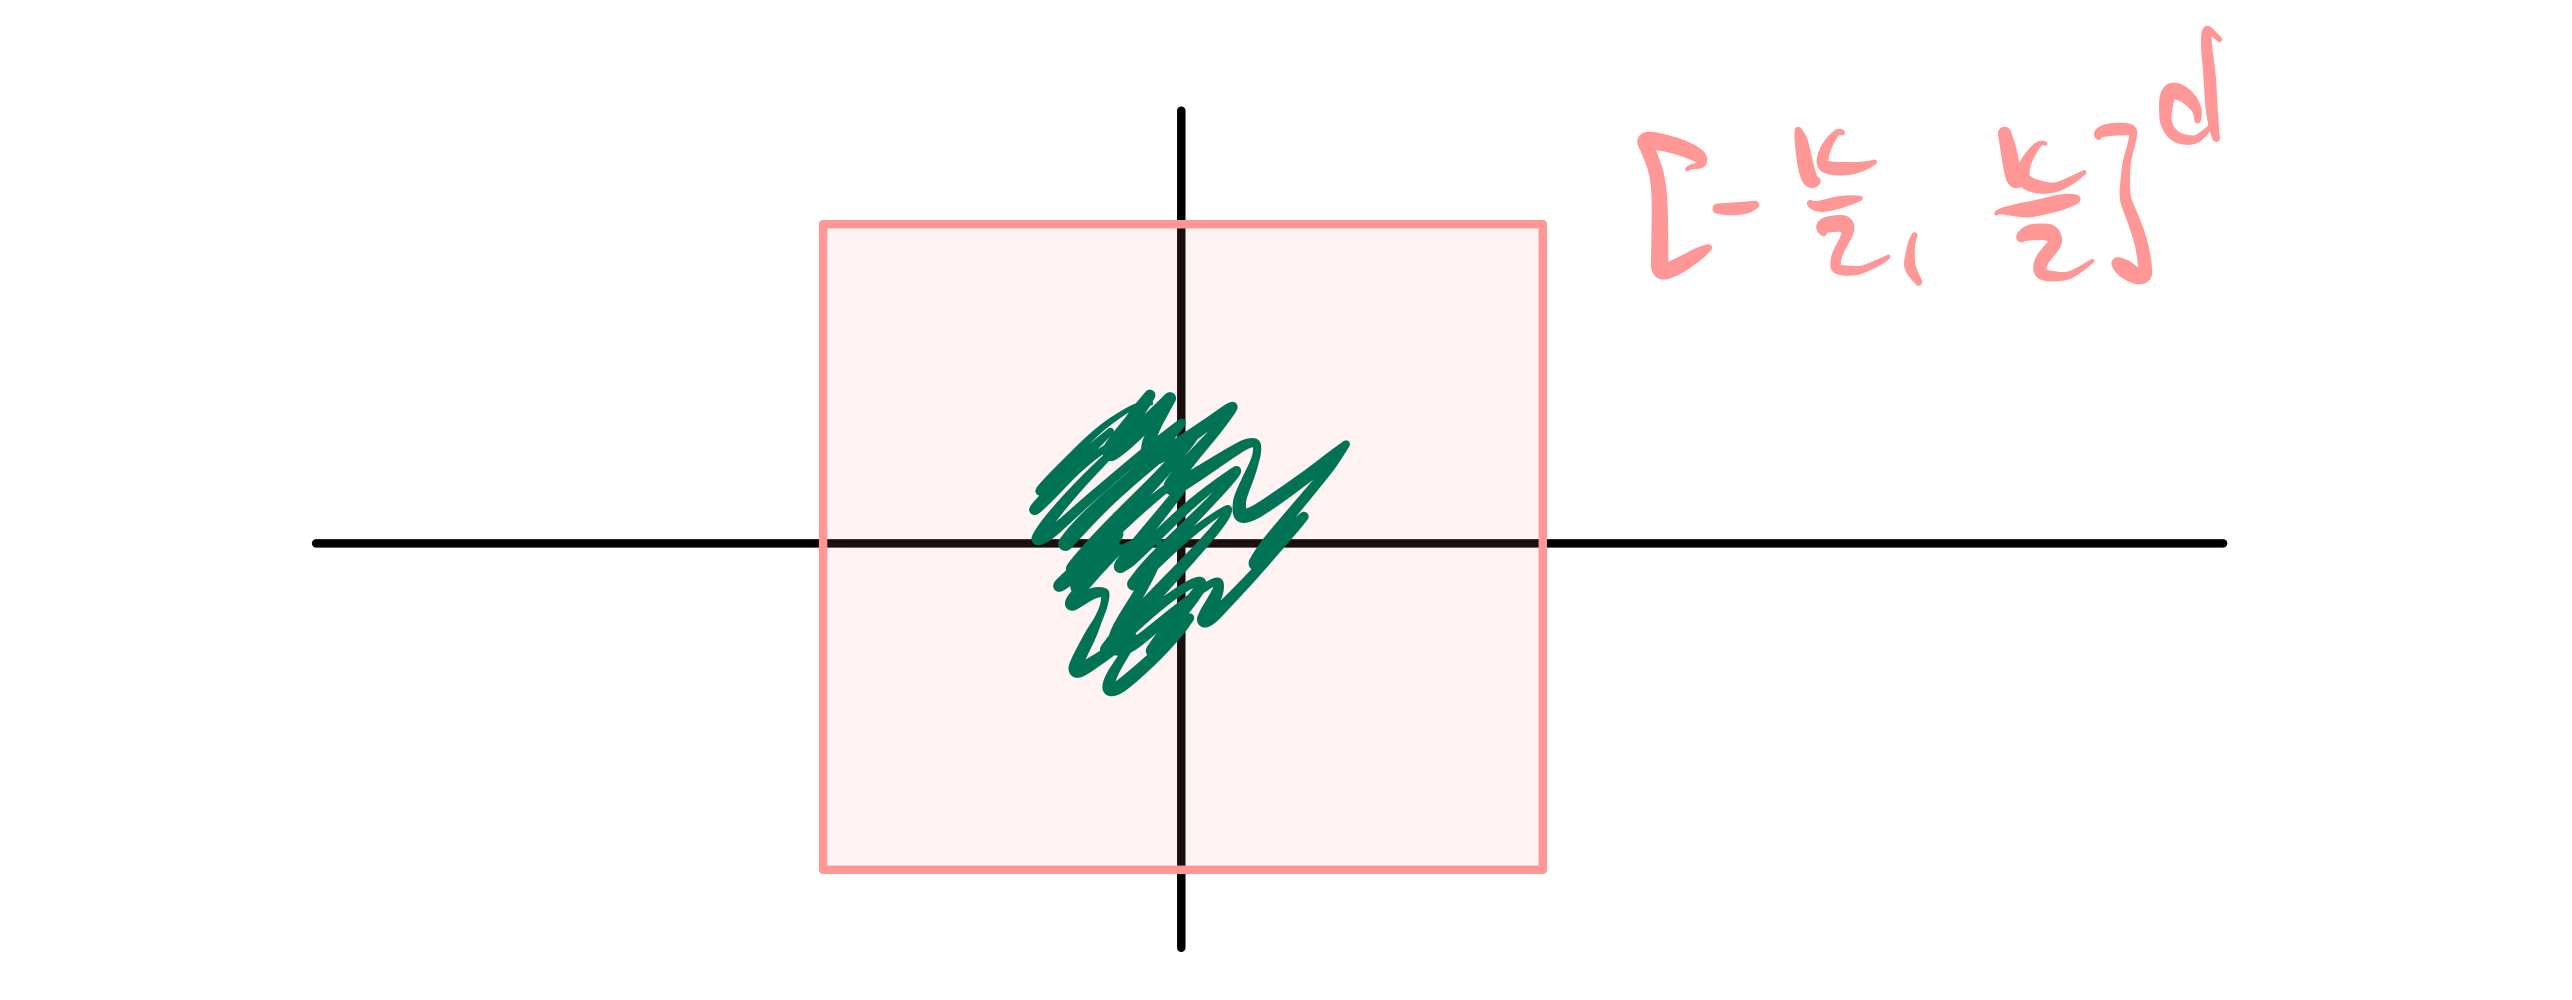
\includegraphics[scale=0.07]{compact.jpeg}
		\end{center}
		\vspace{-3mm}
		\caption*{The support of $f$}
		\end{figure}
	By enlarging $k$ we can choose $k$ such that $\mu_i \big( \mathbb{R}^d  \setminus (k,k)^d \big) < \varepsilon$ for a fixed $\varepsilon >0$ (continuity of measures or Proposition \ref{prop_4120}). Next we define
	\begin{align*}
		g_m \colon \mathbb{R}^d \to \mathbb{C},\quad g_m (x) = e^{ i \langle \frac{\pi m}{k}, x \rangle },\quad m \in x,\mathbb{Z}^d,
	\end{align*}
	and $C_k$ as the algebra of finite linear combinations of the $g_m$. Here is the important point of the functions $g_m$, they are periodic. For $n \in \mathbb{Z}^d$ they satisfy
			\begin{align*}
				g_m(x+2 k n) = e^{ i \langle \frac{\pi m}{k}, x \rangle } \cdot \underbrace{e^{ i \langle \frac{\pi m}{k}, 2k n \rangle }}_{=1} = g_m(x),
			\end{align*}
			as $e^{2\pi l}=1$ for all $l\in\Z$.	Hence, the entire family $C_k$ is periodic!
			\begin{figure}[h]
				\vspace{-1mm}
				\begin{center}
					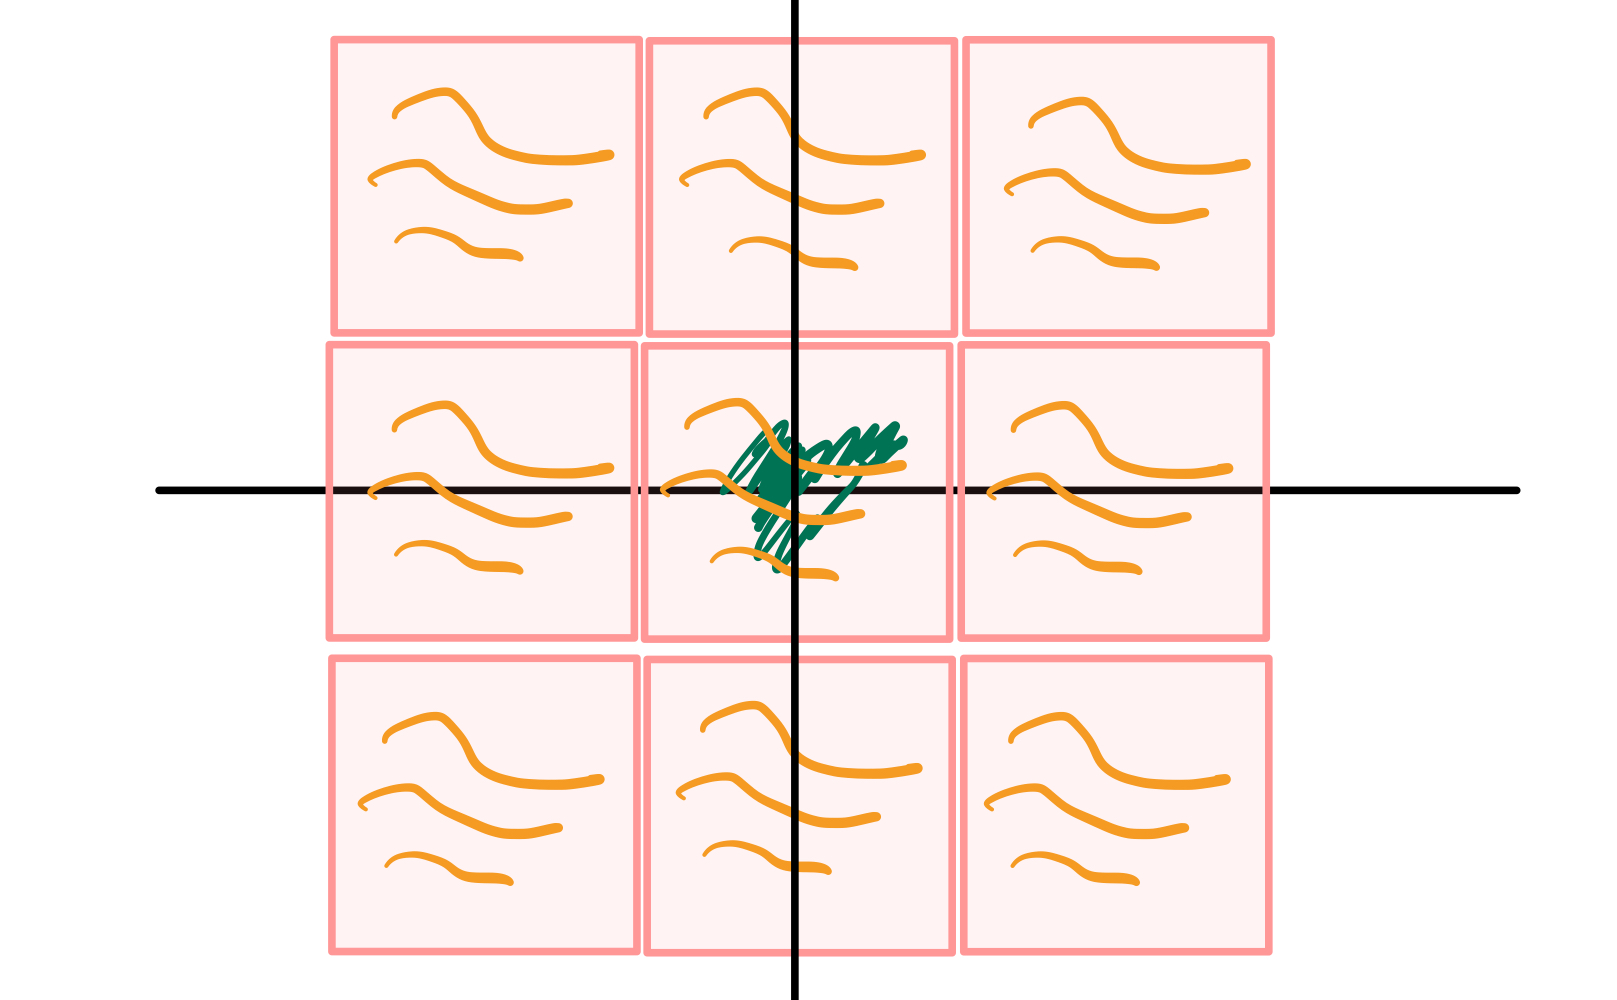
\includegraphics[scale=0.07]{periodic.jpeg}
				\end{center}
				\vspace{-3mm}
				\caption*{Periodic function $g\in C_k$}
				\end{figure}			

			This is important to us as bounding $g\in C_k$ on $[-k,k]^d$ will automatically bound $g$ everywhere. Restricting $C_k$ to $[-k,k]^d$ the class is separating (this needs the $1 /k$ in the scalar product as without it the functions would be periodic for a smaller box taking the same values on shifts of the smaller boxes in the larger box). The Stone-Weierstra\ss{} approximation theorem now implies that there is $g \in C_k$ with 
			\begin{align*}
				\sup_{x\in [-k,k]^d}\lvert f(x) - g(x) \rvert < \varepsilon.
			\end{align*}
			Since $g$ is close to $f$ on $[-k,k]^d$ we can also use the periodicity to bound $g$ on $\R^d$:
			\begin{align*}
				\sup_{x\in\R^d}|g(x)|=\sup_{x\in [-k,k]^d} \lvert g(x) \rvert &\leq \sup_{x\in [-k,k]^d}\lvert f(x) - g(x) \rvert + \sup_{x\in [-k,k]^d} \lvert f(x) \rvert 
					\leq \varepsilon + \left\Vert f \right\Vert_{\infty}.
			\end{align*}
			Putting everything together, the above thoughts yields (please compare the proof of Corollar \ref{cor_514})
			\begin{align*}
				&\quad\Big\lvert \int_{\mathbb{R}^d} f \dint \mu_1 - \int_{\mathbb{R}^d} f \dint \mu_2 \Big\rvert \\
				&\leq \Big\lvert \int_{\mathbb{R}^d} f \dint \mu_1 - \int_{\mathbb{R}^d} g \dint \mu_1 \Big\rvert + \underbrace{ \Big\lvert \int_{\mathbb{R}^d} g \dint \mu_1 - \int_{\mathbb{R}^d} g \dint \mu_2 \Big\rvert }_{= 0 \text{ by assumption}} + \Big\lvert \int_{\mathbb{R}^d} g \dint \mu_2 - \int_{\mathbb{R}^d} f \dint \mu_2 \Big\rvert  \\
&\leq \int_{[k,k]^d}|f-g|\dint \mu_1+ \int_{([k,k]^d)^c}|f-g|\dint \mu_1+ \int_{[k,k]^d}|f-g|\dint \mu_2+ \int_{([k,k]^d)^c}|f-g|\dint \mu_2\\
				& \leq \mu_1 \big( [-k,k]^d \big) \cdot \varepsilon + \mu_1 \big( ([-k,k]^d)^c \big) \cdot ( \varepsilon + \left\Vert f \right\Vert_{\infty}) 
				 +   \mu_2 \big( [-k,k]^d \big)
				+ \mu_2 \big( ([-k,k]^d)^c \big) \cdot ( \varepsilon + \left\Vert f \right\Vert_{\infty}) \\
				&\leq 2 \varepsilon + 2 \varepsilon \big( \varepsilon + \left\Vert f \right\Vert_{\infty} \big).
			\end{align*}
			For the inequalities we used that $\mu_i$ are probability measures, $|f-g|\leq |f|+|g|$, and that $\mu_i$ only have mass at most $\varepsilon$ outside of the chosen box. Since $\varepsilon$ was arbitrary we proved $\int f \dint \mu_1 = \int f \dint \mu_2$.\smallskip

			The second claim follows from the first claim applied to the laws $\P_X$.
\end{proof}
Of course one might ask why one might be interested in computing moments (for bounded random variables) or Laplace transformations (for non-negative random variables) if there is one general theorem that states that characteristic functions uniqueley determine all real random variables. This is because it is easier to compute moments or Laplace transformations these are the preferred tools in the special situations when they are sufficiently powerful.\smallskip

\begin{lwarnhinweis}
So far we are used to describe random variables through their cummulative distribution function, density, or discrete probability weights. An alternative way is to describe random variables directly in terms of their chracteristic functions, which, according to the previous theorem, is as good as using the CDF.
\end{lwarnhinweis}
The drawback of using characteristic functions is that one needs to compute expectations (integrals) for complex functions. At the same time this is the big advantage, too, as complex integration has wonderful tricks to offer. \smallskip

In many examples the uniquneness is applied as follows. In order to identify the distribution of a random variable (such as a sum of other random variables) one tries to compute the characteristic function. If that characteristic function is already known we can identify the law. We already know this concept from Proposition \ref{P7} and the example below but always used the trick without a proof. Here is another little exercise to play with the examples, Lemma \ref{lemma_5111} and uniqueness theorem.
\begin{luebung}
	Check that 
	\begin{itemize}
		\item If $Y\sim \mathcal N(0,1)$, then $Y:=\sigma X+Y\sim \mathcal N(\mu,\sigma^2)$.
		\item
		If $X \sim \cN(\mu_1,\sigma_1^2)$ and $Y \sim \cN(\mu_2,\sigma_2^2)$ are independent, then $$X+Y \sim \cN(\mu_1+\mu_2, \sigma_1^2 + \sigma_2^2).$$
	\item
		If $X \sim \text{Poi}(\lambda)$ and $Y \sim \text{Poi}(\beta)$ are independent, then $X + Y \sim \text{Poi}(\lambda + \beta)$. 
	\end{itemize}
\end{luebung}



\section[Weak convergence on $\mathcal B(\R)$]{Weak convergence on $\mathcal B(\R^d)$}
We can finally return to the question of weak convergence. Recall from Propositon \ref{most_useful_characterization_weak_convergence} that a sequence of probability measures $(\mu_n)$ converges weakly to $\mu$ (equivalently a sequence of random variables $(X_n)$ converges in distribution to $X$) if and only if
\begin{enumerate}[label=(\roman*)]
	\item $\{\mu_n:n\in\N\}$ is tight,
	\item $ \lim_{n\to\infty} \int_E f \dint \mu_n = \int_E f \dint \mu$ for \underline{some} separating family $C \subseteq C_b(E)$ of $\cM_1(E)$.
\end{enumerate}
We have identified separating families in the previous section. It now remains to identify situations in which the tightness trivially holds (bounded and non-negative) and give a handable criterion to check the tightness (convergence of characteristic functions). We keep the order of the previous section and first deal with the simple cases:
\begin{lsatzwichtig}
\begin{theorem}
	\begin{enumerate}[label=(\roman*)]
		\item Suppose that $\mu,\mu_1,...\in \mathcal M_1([a,b])$, then 
	\begin{align*}
		\mu_n \overset{\text{(w)}}{\longrightarrow} \mu,\: n \to \infty \quad\Leftrightarrow \quad \lim_{n\to\infty}\int_{[a,b]} x^m\dint \mu_n(x)=\int_{[a,b]} x^m\dint \mu(x),\quad \forall m\in\N_0.
	\end{align*}
	\item Suppose that $X,X_1,...$ are random variables with values in $[a,b]$, then 
	\begin{align*}
		X_n \overset{\text{(d)}}{\longrightarrow} X,\: n \to \infty \quad\Leftrightarrow \quad \lim_{n\to\infty}\E[X_n^m]=\E[X^m], \quad \forall m\in\N_0.
	\end{align*}
\end{enumerate}
\end{theorem}
\end{lsatzwichtig}
\begin{proof}[Proof]
	(ii) follows from (i) by the definition of convergence in distribution with the measures $\mu_n:=\P_{X_n}$ using that $\E[X_n^m]=\int x^m \dint \P_{X_n}(x)$.\smallskip

	(i) The situation is simple as $([a,b],|\cdot|)$ is compact. Hence, every sequence of measures is automatically tight (choose $K=[a,b]$ in the definition of tightness). According to Proposition \ref{most_useful_characterization_weak_convergence} only convergence of integrals needs to be checked for a separating family. Since the family of monomials $C=\{x^m:m\in\N_0\}$ is separating according to Theorem \ref{coruniq} the proof is complete.
\end{proof}

The situation is very similar for non-negative (or non-positive) sequences of random variables. In contrast to bounded sequences we now need convergence of the exponential moments (Laplace transformation):
\begin{lsatzwichtig}
	\begin{theorem}
		\begin{enumerate}[label=(\roman*)]
			\item Suppose that $\mu,\mu_1,...\in \mathcal M_1([0,\infty))$, then 
		\begin{align*}
		\hspace{-4mm}	\mu_n \overset{\text{(w)}}{\longrightarrow} \mu,\: n \to \infty \quad\Leftrightarrow \quad \lim_{n\to\infty}\int_{[0,\infty)} e^{-\lambda x}\dint \mu_n(x)=\int_{[0,\infty)} e^{-\lambda x}\dint \mu(x),\,\, \forall \lambda >0.
		\end{align*}
		\item Suppose that $X,X_1,...$ are non-negative random variables, then 
		\begin{align*}
			X_n \overset{\text{(d)}}{\longrightarrow} X,\: n \to \infty \quad\Leftrightarrow \quad \lim_{n\to\infty} L_{X_n}(\lambda)=L_X(\lambda), \quad\forall \lambda>0.
		\end{align*}
	\end{enumerate}
	\end{theorem}
	\end{lsatzwichtig}
	\begin{proof}[Proof]
		(ii) follows from (i) by the definition of convergence in distribution with the measures $\mu_n:=\P_{X_n}$ using that $L_{X_n}(\lambda)=\int e^{-\lambda x} \dint \P_{X_n}(x)$.\smallskip
	
		(i) We argue as in the proof of Theorem \ref{cor_distributions_1}. Compactifying $[0,\infty]$ and extending the measures trivially to measures $\bar \mu_n$ yields a sequence of measures in a compact space. As in the previous proof the sequence is automatically tight (choose $K=[0,\infty]$). 
		According to Proposition \ref{most_useful_characterization_weak_convergence} only convergence of integrals needs to be checked for a separating family. Since the family of exponentials $C\coloneqq \{ f_{\lambda} \colon \lambda > 0 \}$ is separating according to Theorem \ref{cor_distributions_1} the proof is complete.
	\end{proof}
The most general theorem is L\'evy's continuity theorem. Without any further assumption weak convergences is equivalent to convergence of the characteristic functions. 
%Erst beschränkt und positiv. Dann R. Dann C.

%\textbf{Goal:}
%	\begin{align*}
%		X_n \overset{(d)}{\longrightarrow} X, \: n\to \infty \: &\Leftrightarrow \: F_{X_n} \longrightarrow F, \: n\to \infty, \text{ at points of continuity} \\
%		&\overset{?}{\Leftrightarrow} \varphi_{X_n} \longrightarrow \varphi_X, \: n \to \infty
%	\end{align*}
%	\begin{lemma1}
%		Let $\mu \in M_1( \mathbb{R}^d)$, then
%		\begin{align*}
%			\lvert \varphi_{\mu}(t) - \varphi_{\mu}(s) \lvert^2 \leq 2 \cdot \big( 1 - \mathcal{R}e( \varphi_{\mu}(t-s)) \big), \:\: \forall s,t 
%		\end{align*}
%	\end{lemma1}
%	\begin{proof}
%		$L^2(\Omega,\cA,\mathbb{P})$ is a Hilbertspace with $\langle f, g \rangle = \int f \cdot \bar{g} \dint \mu$ also if we consider $f \colon \Omega \to \mathbb{C}$ and the complex integral $\int f \dint \mu \coloneqq \int \cR e(f) \dint \mu + i \int Im(f) \dint \mu$.
%		\begin{align*}
%			\big\lvert \varphi_{\mu}(t) - \varphi_{\mu}(s) \big\rvert^2 &= \Big\lvert \int_{\mathbb{R}^d} \big( e^{i \langle t,x \rangle}- e^{i \langle s,x \rangle} \big) \dint \mu (x) \Big\rvert^2 \\
%			&= \Big\lvert \int_{\mathbb{R}^d} \big( e^{i \langle t,x \rangle} - 1 \big) e^{i \langle s, x \rangle} \dint \mu(x) \Big\rvert^2 \\
%			\overset{ \text{C-S}}&{\leq} \int_{\mathbb{R}^d} \lvert e^{ i \langle t-s,x \rangle} - 1 \rvert^2 \dint \mu(x) \cdot \underbrace{\int_{\mathbb{R}^d} \underbrace{\lvert e^{i \langle s,x \rangle} \rvert^2}_{=1} \dint \mu(x) }_{=1} \\
%			\overset{\lvert z \rvert^2 = z \cdot \overline{z}}&{=} \int_{\mathbb{R}^d} \big( e^{i \langle t - s, x \rangle} - 1\big) \cdot \big( e^{-i \langle t-s,x \rangle} - 1 \big) \dint \mu(x) \\
%			&= 2 \cdot \big(1 - \cR e(\varphi_{\mu}(t-s)) \big)
%		\end{align*}
%	\end{proof}
%	Recall: $f \colon E \to F$ is uniformly continuous if $\forall \varepsilon > 0 \exists \delta > 0 \colon \: d(x,y) <\delta \Rightarrow d \big( f(x),f(y) \big) < \varepsilon$. Now we take a family of continuous functions and wanr the choice of $\delta$ to be the same for all $f$ $\rightsquigarrow$ family $\cF$ is uniformly uniformly continuous.
%	\begin{deff1}
%		Let $(E,d)$ be a metric space. A family $(f_i)_{i\in I}$ of maps $f_i \colon E \to \mathbb{R}$ is called \underline{\smash{uniformly equicontinuous}} if
%		\begin{align*}
%			\forall \varepsilon > 0 \: \exists \delta > 0 \colon \: d(x,y) < \delta \: \Rightarrow \: \lvert f_i(x) - f_i(y) \rvert < \delta \:\: \forall i \in I
%		\end{align*}
%	\end{deff1}
%	\begin{theorem}
%		If $\cF \subseteq M_1( \mathbb{R}^d ) $ is tight, then $\{ \varphi_{\mu} \colon \mu \in \cF \}$ is uniformly equicontinuous. In particular, every characteristic function is uniformly continuous.
%	\end{theorem}
%	\begin{proof}
%		Recall $\big( M_1(\mathbb{R}^d), d_P \big)$ is indeed a metric space (even Polish). Fix $\varepsilon > 0$. Since $\cF$ is tight there is $N\in \mathbb{N}$ with $\mu \big( [ -N, N ]^d \big) > 1- \frac{\varepsilon^2}{6}$. Since $[-N,N]^d$ is compact there is a $\delta > 0$ such that $ \lvert 1 - e^{i \langle u,x \rangle} \rvert < \frac{\varepsilon^2}{6}$ for all $x \in [-N,N ]^d$ and all $\lvert u \rvert < \delta$ (Use continuity of $(u,x) \mapsto 1 - e^{i \langle u,x \rangle}$ and cover with finitely many balls, take the smallest corresponding $\delta$ which then works for all $x$ at onexe). Hence,
%		\begin{align*}
%			1 - \cR e  \big( \varphi_{\mu}(u) \big) &\leq \int \lvert 1 - e^{i \langle u,x \rangle} \rvert \dint \mu(x) \\
%			&\leq 2 \cdot \mu \big( ([-N,N]^d)^C \big) + \frac{\varepsilon^2}{6} \mu \big( [-N,N]^d \big)  \\
%			&\leq \frac{\varepsilon^2}{3} + \frac{\varepsilon^2}{6} = \frac{\varepsilon^2}{2}
%		\end{align*}
%		for all $\mu \in \cF$. Now we use the lemma to get the uniform bound needed for the definition of uniformly equicontinuity.
%	\end{proof}
%	\begin{prop1}[limits of uniformly uniformly seq. of functions are unif. cont.]
%		Let $(E,d)$ be a metric space, $f,f_1,f_2,...\colon E \to \mathbb{R}$ with $f_n \to f$ pointwise. If $(f_n)_{n\to\infty}$ is uniformly equicontinuous, then
%			\begin{enumerate}[label=(\roman*)]
%				\item $f$ is uniformly continuous
%				\item $f_n \to f$ uniformly on compacts, i.e. $\sup\limits_{x\in K} \lvert f_n(x) - f(x) \rvert \to 0$ for all $K \subseteq E$ compact.
%			\end{enumerate}
%	\end{prop1}
%	\begin{proof}
%		\begin{enumerate}[label=(\roman*)]
%			\item
%				Let $\varepsilon >0$ and fix $\delta >$ with $\lvert f_n(x) - f_n(y) \rvert < \varepsilon$ for all $x,y\in E$ with $d(x,y) < \delta$. Then 
%				\begin{align*}
%					\lvert f(x) - f(y) \rvert  = \lim_{n\to \infty} \lvert f_n(x) - f_n(y) \rvert < \varepsilon
%				\end{align*}
%				for those $x,$ $y,$. Hence, $f $ is uniformly continuous.
%			\item
%				Trick: Cover $K$ wtih finitely many balls. Let $\varepsilon > 0$ and chose $\delta$ from the uniform equicontinuity. Now conver $K$ by $B_{\delta}(t_1),...,B_{\delta}(t_N)$ which is possible as all compact sets are totally bounded. Now choose $n_0$ large enough so that
%				\begin{align*}
%					\lvert f_n (t_1) - f(t_1) \rvert < \varepsilon, ...., \lvert f_n(t_N) - f(t_N) \rvert < \varepsilon \:\: \forall n \geq n_0.
%				\end{align*}
%				For $x \in K$ choose a $t_i$ with $x \in B_{\delta}(t_i)$. Then
%				\begin{align*}
%					\lvert f_n(x) - f(x) \rvert &\leq \lvert f_n(x) - f_n(t_i) \rvert + \lvert f_n(t_i) - f(t_i) \rvert + \lvert f(t_i) - f(x) \rvert \\
%					&\leq \varepsilon + \varepsilon + \varepsilon
%				\end{align*}
%				which gives $\sup\limits_{x\in K} \lvert f_n(x) - f(x) \rvert < 3 \varepsilon$. That's it!
%		\end{enumerate}
%	\end{proof}
		\marginpar{\textcolor{red}{Lecture 17}}



		\begin{lsuperwichtigersatz}
			\begin{theorem}[L\'{e}vy's continuity theorem]\label{levy_special}
				\begin{enumerate}[label=(\roman*)]
					\item Suppose that $\mu,\mu_1,...\in \cM_1(\mathbb{R}^d)$, then
					\begin{align*}
						\mu_n \overset{\text{(w)}}{\longrightarrow} \mu,\: n \to \infty \quad\Leftrightarrow \quad \lim_{n\to\infty} \varphi_{\mu_n} = \varphi_\mu(t), \quad \forall t \in \mathbb{R}^d.
					\end{align*}
					\item Suppose that $X,X_1,...$ are $\R^d$-valued random variables, then
						\begin{align*}
						X_n \overset{\text{(d)}}{\longrightarrow} X, \: n \to \infty \quad \Leftrightarrow \quad \lim_{n\to\infty}\varphi_X(t) = \varphi_X(t), \quad \forall t \in \mathbb{R}^d.
					\end{align*}				
				\end{enumerate}
			\end{theorem}
		\end{lsuperwichtigersatz}
\begin{proof}[Proof]
As earlier we only prove (i) as (ii) follows directly using $\mu_n=\P_{X_n}$.\smallskip

"$\Rightarrow$": Since $g = e^{i \langle t, \cdot \rangle}=\cos(\langle t,\cdot\rangle)+i\sin(\langle t,\cdot\rangle)$ and $\cos,\sin\in C_b(\mathbb{R}^d)$ the pointwise convergence follows from the definition of weak convergence.\smallskip

"$\Leftarrow$": We will actually prove a stronger statement than claimed, the so-called general continuity theorem:
\begin{lwarnhinweis}
	Suppose $\lim_{n\to\infty}\varphi_{\mu_n}(t)= f(t)$, for all $t\in\R^d$, where $f \colon \mathbb{R}^d \to \mathbb{C}$ is continuous at $0$. Then there is a probability measure $Q$ on $\cB(\R^d)$ with $f = \varphi_Q$ and $\mu_n \overset{\text{(w)}}{\longrightarrow} Q, \: n\to \infty$.
\end{lwarnhinweis}
Once we proved the general continuity theorem we immediately get the special continuity theorem by chosing $f=\varphi_\mu$ which is continuous at $0$ by dominated convergence $(|e^{i\langle t,X\rangle}|=1)$.\smallskip

Comparing with the proofs of the previous two theorems the strategy is as follows:
\begin{itemize}
	\item deduce tightness of $(\mu_n)$,
	\item find a separating sequence for which the integrals converge,
\end{itemize}
because then the claim follows from Proposition \ref{most_useful_characterization_weak_convergence}. Chosing $C:=\{e^{i\langle t,x\rangle}: t\in\R\}$ we already proved in Theorem \ref{CF} that $C$ is separating. Hence, we need to prove that the assumed pointwise convergence of $\varphi_{\mu_n}$ implies tightness of $(\mu_n)$.\smallskip

To do so let us first check that without loss of generality we may assume $d=1$. If $\pi_k(x)=x_k$ denotes the projection on the $k$th coordinate, then we define $\mu_n^k:= \mu_n\circ \pi_k$, the push-forward of the measures on the coordinates. Their characteristic functions of $\mu_n^k$ can be expresses through the characteristic functions of $\mu_n$:
\begin{align*}
	\varphi_{\mu_n^{k}}(t) = \int_{\mathbb{R}} e^{ixt} \dint \mu_n^k(x)
		=  \int_{\mathbb{R}} e^{i \langle x , t  \text{e}_k \rangle} \dint \mu_n(x)
		= \varphi_{\mu_n}(t  \text{e}_k),\quad t\in\R.
\end{align*}
Hence, the assumed pointwise convergence of $\varphi_{\mu_n}$ implies the convergence of all $\varphi_{\mu_n^k}$. If now we can prove that this implies tightness for all $(\mu_n^k)_{k\in\N}$, then, using Prohorov's characterisation of tightness through sequences, we obtain tightness of $(\mu_n)_{n\in\N}$. BECUASE.\smallskip 

From now on we assume $d=1$ and that $(\varphi_{\mu_n})_{n\in\N}$ converges pointwise to a function $f$ that is continuous at $0$. 
%\end{proof}
%\begin{lsuperwichtigersatz}
%	\begin{theorem}[L\'{e}vy continuity theorem, general formulation]\label{levy_general}
%		Let $\mu, \mu_1,...\in M_1(\mathbb{R}^d)$.
%		\begin{enumerate}[label=(\roman*)]
%			\item
%				$\mu_n \overset{\text{(w)}}{\longrightarrow} \mu, \: n\to \infty \: \Rightarrow \: \varphi_{\mu_n}(t)\to \varphi_\mu(t),\: n\to\infty,\quad \forall t\in\R.$
%			\item
%				If $\varphi_{P_n} \to f$, $n \to \infty$, pointwise for some $f \colon \mathbb{R}^d \to \mathbb{C}$ that is (partially) continuous at $0$, then there is a probability measure $Q$ on $\cB(E)$ with $f = \varphi_Q$ and $P_n \overset{\text{(w)}}{\longrightarrow} Q, \: n\to \infty$.
%		\end{enumerate}
%	\end{theorem}
%	\end{lsuperwichtigersatz}
%	Most importantly: $\varphi_{X_n} \to \varphi_X$, $n \to \infty$, pointwise $\Rightarrow$ $X_n \overset{\text{(d)}}{\longrightarrow}X, \: n \to \infty$.
%	\begin{proof}
%		\begin{enumerate}[label=(\roman*)]
%			\item
%				Since $g = e^{i \langle t, \cdot \rangle}=\cos(\langle t,\cdot\rangle)+i\sin(\langle t,\cdot\rangle)$ and $\cos,\sin\in \in C_b(\mathbb{R}^d)$ the pointwise convergence follows from the definition of weak convergence.
				
				
	%			we have $\varphi_{P_n} \to \varphi_P$ pointwise. By Prohorov the sequence is tight, hence, their characteristic functions are uniformly equicontinuous. Thus, by the lemma the convergence is also unif. on compacts. (???)
First recall that						\begin{align*}
	\varphi_{\mu}(t) = \int e^{itx} \dint \mu(x) = \int \cos(tx) \dint \mu(x) + i \int \sin (tx) \dint \mu(x)
\end{align*}
We want to relate tightness (probabilities) to integrals (characteristic functions). Usually we took closed sets $A$ and approximated $\mathbf 1_A$ with $f_A^\varepsilon$. Here we use a different trick by estimating suitiable indicators from above by the sine/cosine functions. Define $h \colon \mathbb{R} \to [0, \infty)$ as 
							\begin{align*}
								h(x) = \begin{cases}
									1 - \frac{\sin(x)}{x} &: x \neq 0 \\
									0 &: x = 0 \end{cases},
							\end{align*}				
						which is non-negative and continuous on $\mathbb{R}$ (Analysis):
							\begin{figure}[h]
							\begin{center}
								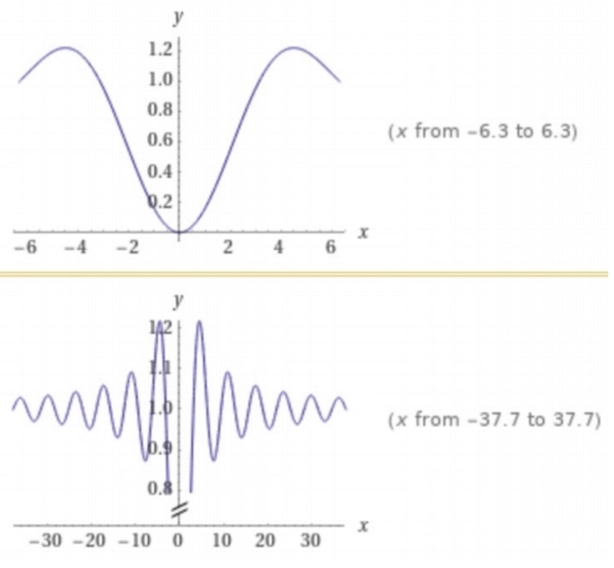
\includegraphics[scale=0.3]{bild.jpg}
							\end{center}
							\end{figure}
						
							Now define 
						 $$\alpha \coloneqq \inf \{ h(x) \colon \lvert x \rvert \geq 1 \} = 1 -\sin(1) > 0$$ so that $\frac{h(x)}{\alpha}\geq 1$ for $|x|>1$. Then, for $k\geq 1$,
		\begin{align*}
			\mu_n \big( [-k,k]^c \big) \overset{\text{mon.}}&{\leq} \int_{[-k,k]^c} \frac{1}{\alpha} h \Big( \frac{x}{k} \Big) \dint \mu_n(x) \\
			&\leq \frac{1}{\alpha} \int_{\mathbb{R}} h \Big( \frac{x}{k} \Big) \dint \mu_n(x) \\
			&= \frac{1}{\alpha} \int_{\mathbb{R}} \underbrace{\bigg( \int_0^1 \Big( 1 - \cos \Big( \frac{t x}{k}\Big) \Big) \dint t \bigg)}_{=1- \sin(\frac{x}{k}) \frac{k}{x} = h(\frac{x}{k})} \dint \mu_n(x) \\
			\overset{\text{Fubini}}&{=} \frac{1}{\alpha} \int_0^1 \int_{\mathbb{R}} \Big( 1 - \cos \Big( \frac{t x}{k} \Big) \Big) \dint \mu_n(x) \dint t \\
			&= \frac{1}{\alpha} \int_0^1 \Big( 1  - \cR e \Big( \varphi_{\mu_n} \Big( \frac{t}{k} \Big) \Big) \Big) \dint t.
		\end{align*}	
						Now we use dominated convergence to obtain
						\begin{align*}
							\limsup_{n\to\infty} \mu_n \big( [-k,k]^c \big) &\leq \frac{1}{\alpha} \lim_{n\to\infty} \int_0^1 \Big( 1 - \cR e \Big( \varphi_{\mu_n} \Big( \frac{t}{k} \Big) \Big) \big) \dint t \\
						\overset{\text{DCT}}&{=} \frac{1}{\alpha} \int_0^1 \lim_{n \to \infty}  \bigg( 1 - \cR e \Big( \varphi_{\mu_n} \Big( \frac{t}{k} \Big) \Big) \bigg) \dint t \\
							&= \frac{1}{\alpha} \int_0^1  \Big( 1 - \cR e \Big( f \Big( \frac{t}{k} \Big) \Big) \Big)
						\end{align*}	
						In the last step we have used that convergence of a sequence of complex numbers implies convergence of real- and imaginary-parts.			
						Finally, we use the continuity of $f$ (and thus $\cR e(f)$) at $0$. For all $\varepsilon > 0$ there is a $\delta>0$ such that $\lvert 0 - \frac{t}{k} \rvert < \delta$ implies $\lvert 1 - \cR e ( f(\frac{t}{k})) ) \rvert = \lvert \cR e(f(0)) - \cR e ( f(\frac{t}{k})) ) \rvert \leq \varepsilon$. Hence, there is some $k$ so that $\lvert 1 - \cR e ( f(\frac{t}{k})) ) \rvert < \varepsilon$ for all $t \in [0,1]$. But then there is some $k$ so that $\limsup_{n\to\infty} \mu_n \big( [-k,k]^c \big) < \varepsilon$. 
				
						From this the tightness follows as every single probability measure on $\mathbb{R}^d$ is tight. ARGUMENT HINSCHREIBEN
	\end{proof}
	%\begin{lsuperwichtigersatz}
	%\begin{corollary}[L\'{e}vy continuity theorem - special formulation]\label{levy_special}
	
	%	\begin{enumerate}[label=(\roman*)]
	%		\item		Suppose $\mu,\mu_1,...\in \cM_1(\mathbb{R}^d)$, then
	%		\begin{align*}
	%			\mu_n \overset{\text{(w)}}{\longrightarrow} \mu,\: n \to \infty \quad\Leftrightarrow \quad \varphi_{\mu_n} \to \varphi_\mu(t),\: n \to \infty,  \quad \forall t \in \mathbb{R}.
	%		\end{align*}
	%		\item Suppose $X,X_1,...$ are $\R^d$-valued random variables, then
	%			\begin{align*}
	%			X_n \overset{\text{(d)}}{\longrightarrow} X, \: n \to \infty \quad \Leftrightarrow \quad \varphi_X(t) \to \varphi_X(t),\: n \to \infty, \quad \forall t \in \mathbb{R}.
	%		\end{align*}				
	%	\end{enumerate}
	%\end{corollary}			
%\end{lsuperwichtigersatz}

We finish the section with a short discussion of the usefulness of the generalised version of the continuity theorem. Let us recall the different ways of characterising random variables: 
\begin{align*}
	\text{random variable }X\quad \Leftrightarrow \quad \text{ law }\P_X\quad \Leftrightarrow \quad \text{CDF }F_X.
\end{align*}
In fact, just as CDFs are functions with a set of properties one can ask if also characteristic functions are functions with a set of axiomatic properties so that it is reasonable to extend 
\begin{align*}
	\text{random variable }X\quad \Leftrightarrow \quad \text{ law }\P_X\quad \Leftrightarrow \quad \text{CDF }F_X\quad \Leftrightarrow\quad \text{characteristic function }\varphi_X.
\end{align*}
Indeed, this is the case but unfortunately the appearing property of positive definitness is hard to check:
\begin{lsatz}
\begin{theorem}[Bochner]
	A function $\varphi \colon \mathbb{R}^d \to \mathbb{C}$ is the characteristic function of a random vector (or a probability measure on $\mathcal B(\R^d)$) if and only if 
	\begin{itemize}
		\item $\varphi(0)=1$
		\item $\varphi$ is continuous at $0$
		\item $\varphi$ is \textbf{positive semidefinite}, i.e. 
		\begin{align*}
			\sum_{k,l=1}^{n} y_k \bar{y}_l \varphi(t_k - t_l) \geq 0, \quad \forall n \in \mathbb{N}, \: t_i \in \mathbb{R}^d, \: y_i \in \mathbb{C}.
		\end{align*}	
	\end{itemize}
\end{theorem}
\end{lsatz}
\begin{proof}[Proof]
	"$\Rightarrow$": Suppose $\varphi(t)=\E[e^{itX}]$ for some random variable $X$. Then $\varphi(0) = 1$ is clear, continuity at $0$ follows from dominated convergence, and
		\begin{align*}
			\sum_{k,l=1} y_k \bar{y}_l \varphi (t_k - t_l) &= \sum_{k,l=1} y_k \bar{y}_l \int_{\mathbb{R}^d} e^{i \langle x, t_k - t_l \rangle} \dint \mu(x) \\
				&= \int_{\mathbb{R}^d} \sum_{k,l=1}^n y_k e^{i \langle x ,t_k \rangle} \overline{y_l e^{i \langle x ,t_l \rangle}} \dint \mu(x) \\
				&= \int_{\mathbb{R}^d} \Big\lvert \sum_{k=1} y_k e^{i \langle x , t_k \rangle} \Big\rvert^2 \dint \mu(x) \geq 0.
		\end{align*}
	"$\Leftarrow$": Too hard
\end{proof}
There are many classes of characteristic functions that can be understood more directly using the general version of the continuity theorem. If for some reason we have a sequence of characteristic functions $\varphi_n$ that converges pointwise to a function $\varphi$ that is continuous at $0$, then $\varphi$ is a characteristic function. For all even continuous functions $\varphi \colon \mathbb{R} \to [0,1]$ with $\varphi(0)=1$ that are convex on $[0,\infty)$ this can be done (P\'olya's theorem). One can in fact construct simple explicit random variables which characteristic functions $\varphi_n$ that are  approximations of such such functions and converge pointwise to $\varphi$.

\begin{figure}[h]
	\begin{center}
		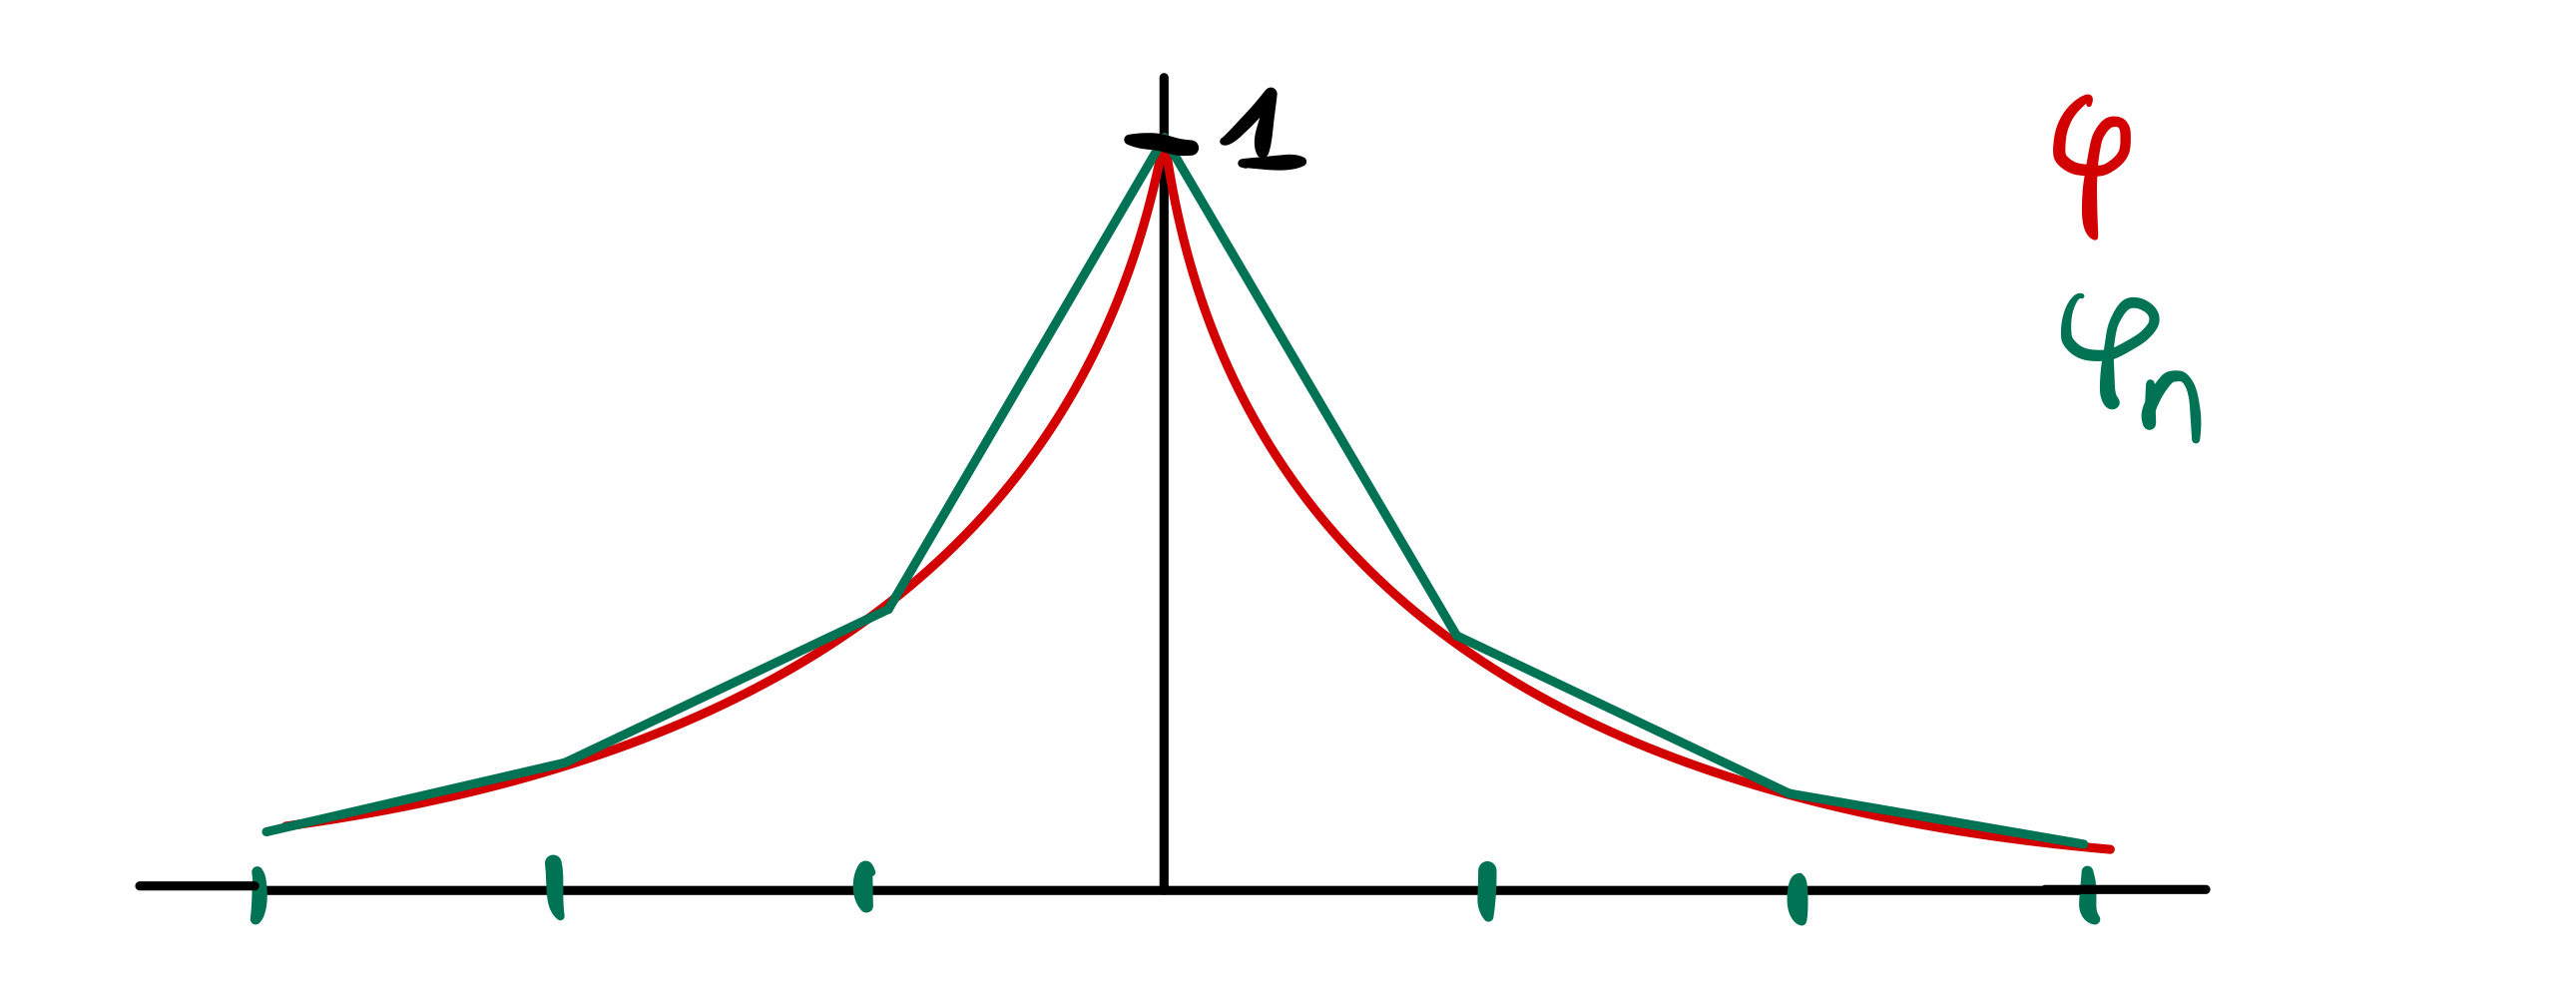
\includegraphics[scale=0.07]{characteristic.jpeg}
	\end{center}
	\vspace{-9mm}
	\end{figure}



\begin{example}
	For $\alpha\in (0,1)$ and $\lambda>0$ the function $\varphi_{\alpha}(t) = e^{- \lambda \lvert t \rvert^{\alpha}}$ is even and convex on $[0,\infty)$. By P\'olya's theorem this is a characteristic function of a random variable $X$. The random variable is called $\alpha$-stable. In fact, the assumption $\alpha\in (0,1)$ is only needed to apply P\'olya's theorem, actually $\varphi_\alpha$ is a characteristic function if and only if $\alpha\in [0,2]$. All such random variables are called $\alpha$-stable and generalise the Gaussian distribution which appears for $\alpha=2$.
\end{example}


	\marginpar{\textcolor{red}{Lecture 18}}



\section{Applications}
Recall from Theorem \ref{erzeugende} the relation $\E[X^n]=\frac{\mathcal M_X^{(n)}(0)}{n!}$ between derivatives of the moment generating function $\mathcal M_X(t)=\E[e^{tX}]$ and the moments. The relation is useful as it allows to compute moments easily for a couple of examples (such as the Gaussian). In principle the idea is very simple, here for the first moment: $$\mathcal M'_X(t)=\frac{d}{dt}\E[e^{tX}]=\E\Big[\frac{d}{dt}e^{tX}\Big]=\E[X e^{tX}]$$ and then plugging-in $t=0$. What makes the proof tricky is the interchange of differentiation and expectation for which dominated convergence needs to be applied in the right way and this forced us to assume finiteness of $\mathcal M_X$ in some interval $(-\varepsilon, \varepsilon)$. Since finiteness of $\mathcal M_X(t)$ means existence of exponential moments the theorem looks much better than it is, the assumption is extremely strong! We will now repeat the same story using the complex exponential. Before doing so we should first say a word on differentiation for functions $f:\R\to \C$. This is either defined by interpreting $\C$ as $\R^2$ and then the rewriting the derivative (a vector) in terms of polar coordinates or directly by taking limits in $\C$: $\frac{d}{dt} f(t)=f'(t)=\lim_{h\to 0}\frac{f(t+h)-f(t)}{h}$. Writing 
\begin{align*}
	\lim_{h\to 0}\frac{f(t+h)-f(t)}{h}=\lim_{h\to 0}\frac{\mathcal R ef(t+h)-\mathcal R ef(t)}{h}+i\lim_{h\to 0}\frac{\mathcal I m f(t+h)-\mathcal I mf(t)}{h}
\end{align*}
shows that both approaches give exactly the same. As always it is important to keep in mind that we can freely ignore the formal definition and just compute in $\C$ as we are used to in $\R$ with the convention $i^2=-1$. Most importantly, it holds that $\frac{d}{dt} e^{itx}=ix e^{itx}$. Higher order derivatives are definded recursively and denoted as usually by $f^{(n)}$. Now suppose, as for moment generating functions, the differentiation can be switched into the expectation, then we should get $\varphi_X^{(n)}(t) = \E \big[ i^n X^ne^{itX} \big]$ so that plugging-in $t=0$ gives again a moment formula $\E[X^n]=\frac{\varphi_X^{(n)}(0)}{i^n}$. Here again the magic of the complex exponential occurs. It is equally powerful in terms of what one can get from it but it is much more friendly because it is bounded. In essense the following theorem shows how to replace the real-exponential (moment generating function) by the complex-exponential (characteristic function) to obtain the same kind of results with minimal assumptions on the random variable.
\begin{lsatz}
\begin{theorem}[Moments of $X$ and differentiability of $\varphi_X$]\label{theorem_moments}
	Let $X$ be a real-valued random variable with characteristic function $\varphi_X$.
	\begin{enumerate}[label=(\roman*)]
		\item
			If $\E[ \lvert X^n \rvert ] < \infty$, then $\varphi_X$ is $n$-times continuously differentiable with $$ \varphi_X^{(n)}(t) = \E \big[ e^{itX}i^n X^n \big], \quad t \in \mathbb{R}.$$
			In particular, $\E[X^n]=\frac{\varphi^{(n)}_X(0)}{i^n }$.
		\item
			If $\E [ \lvert X^n \rvert ] < \infty$ for some $n\in\N$, then $\varphi_X$ satisfies the Taylor approximation
			\begin{align}\label{Taylor}
				\varphi_X(t) = \sum_{k=0}^n \frac{i^k \E[X^k]}{k!} t^k + h_n(t)t^2, \quad t\in \mathbb{R},
			\end{align}
			with a residual term satisfying $\lim\limits_{t \to 0} h_n(t) =0$.
		\item
			If $\lim\limits_{k \to \infty} \frac{t^k \cdot \E [ \lvert X^k \rvert ]}{k!} = 0$ for some $t\in\R$, then $\lim_{n\to\infty} h_n(t) =0$. In particular, $\varphi_X$ has the power series representation
			\begin{align*}
				\varphi_X(t) = \sum_{k=0}^{\infty} \frac{i^k \E[X^k]}{k!}t^k,\quad t\in\R.
			\end{align*}
	\end{enumerate}
\end{theorem}
\end{lsatz}
The power series representation of $\varphi_X$ is not surprsing at all. Writing the complex exponential as a power series and exchanging freely expectation and infinite sum this nothing but
\begin{align*}
	\varphi_X(t)=\E\Big[\sum_{k=0}^\infty \frac{i^kt^kX^k}{k!}\Big]=\sum_{k=0}^\infty \frac{i^k\E[X^k]}{k!}t^k.
\end{align*}
Of course, the interchange is non-trivial and there are essentially two ways to go. Either, arguing as in the proof of Theorem \ref{erzeugende} one takes the limit of the partial sums, justifies dominated convergence, and then gets the moment formual by differentiating the power series, or, as we argue below, one first identifies the derivatives and then refers to Taylor's theorem to derive the power series.
\begin{proof}[Proof]
	In order to swich differentiation and expectation we will use the differential quotient and use dominated convergence to justify the change of expectation and limit in $\varepsilon$. We can do this since the differences of complex exponentials have useful bounds. Let us first check the basic estimate  $\lvert e^{itx} - e^{isx} \rvert \leq \lvert t - s \rvert \cdot \lvert x \rvert $. If $s < t$ and $x > 0$, then expanding the exponential and using the Euler formula yields
	\begin{align*}
		\lvert e^{itx} - e^{isx} \rvert &= \lvert e^{is\frac{x}{2}} \rvert \cdot \lvert e^{it\frac{x}{2}} \rvert \cdot \lvert  e^{i(t-s)\frac{x}{2}} - e^{-i(t-s)\frac{x}{2}} \rvert \\
		&= 2 \lvert \sin ((t-s) x/2 ) \rvert \\
		&= 2  \Big\lvert \int_0^{(t-s) \frac{x}{2}} \cos(u)\dint u \Big\rvert
		\overset{|\cos|\leq 1}{\leq} |(t-s)x|
	\end{align*}
	and the other cases are treated similarly.\smallskip
	
	(i) The first derivative is now simple:
			\begin{align*}
				\lim\limits_{h\to 0} \frac{\varphi_X(t)-\varphi_X(t+h)}{h} = \lim\limits_{h \to 0} \E \bigg[ \frac{e^{itx}-e^{i(t+h)x}}{h} \bigg] 
							\overset{\text{DCT}}{=} \E \bigg[ \lim\limits_{h \to 0} \frac{e^{itx}-e^{i(t+h)x}}{h} \bigg] 
							= \E \big[ i  X  e^{itX} \big]
			\end{align*}
			Changing limits and expectation was justified by the integrable (assumption) upper bound
			\begin{align*}
				\bigg\lvert  \frac{e^{itx}-e^{i(t+h)x}}{h} \bigg\rvert  \leq \frac{\lvert h \cdot x \rvert }{\lvert h \rvert} = \lvert x \rvert
			\end{align*}
			which was justified above. Hence, $\varphi_X^{\prime}(t) = \E \big[ e^{itX}i X \big]$ exists. Inductively we proceed in exactly the same way to differentiate $\varphi_X^{(k)}(t)$:
			\begin{align*}
				\lim_{h\to 0} \frac{\varphi_X^{(k)}(t) - \varphi_X^{(k)}(t+h)}{h} &= \lim_{h\to 0} \frac{\E \big[e^{itX}i^k X^k\big] - \E \big[ e^{i(t+h)X}i^k X^k\big]}{h} \\
			&=\lim_{h\to 0} \E \bigg[ \frac{\big( e^{itX - e^{i(t+h)X}}\big) i^k X^k}{h} \bigg] \\
				\overset{\text{DCT}}&{=} \E \bigg[ \lim_{h\to 0} \frac{\big( e^{itX - e^{i(t+h)X}}\big) i^k X^k}{h} \bigg] 
				= \E \big[ i^{k+1} X^{k+1} e^{itX} \big]
			\end{align*}
			The interchange of limit and expectation is again justified by the upper bound
			\begin{align*}
				\frac{\lvert (e^{itx} - e^{i(t+h)x}) i^k x^k \rvert}{h} \leq \lvert x \rvert \cdot \lvert x^k \rvert = \lvert x^{k+1} \rvert.
			\end{align*}
			The proof shows very clearly that $\varphi_X$ can be differentiated as long as there are enough finite moments of $X$. But this is no additional assumption as otherwise the formula does not make sense anyways!\smallskip

	(ii) Since all derivatives at $0$ are known from (i) the complex version of Taylor's theorem for $x_0 =0$ gives
			\begin{align*}
				\varphi_X(t) = 1+  i t \E[X] - \frac{1}{2} t^2 \E [ X^2] + ... + \frac{i^n t^n\E [X^n]}{n!} + R_n(t)t^n,
			\end{align*}
			with a remainder term satisfying $\lim\limits_{t\to 0} h_n(t) = 0$.\smallskip

	(iii)
			We need to show that, for fixed $t$, the residual $h_n(t)$ vanishes as $n$ tends to infinity. It is most practical to use the integral representation for $R_n(t):=h_n(t)t^n$:
			\begin{align*}
				\lvert R_n(t) \rvert = \Big\lvert \int_0^t \frac{\varphi_X^{(n+1)}(s)}{(n+1)!}(t-s)^n \dint s \Big\rvert &\leq \int_0^t \frac{\E [ \lvert X^{n+1}\rvert] }{(n+1)!}(t-s)^n \dint s
				 = \frac{t^{n+1}}{(n+1)} \frac{\E[ \lvert X^{n+1}\rvert ]}{(n+1)!}
			\end{align*}
			Here we used the formula from (i) and that $|e^{itX}i^n|=1$. But then $h_n(t)\to 0$ for $n\to\infty$.
\end{proof}
Just as we used the moment generating functions to compute moments for random variables with exponential moments we can also use the characteristic functions:
\begin{luebung}
	Compute the first few moments of $\mathcal N(0,1)$, $\text{Poi}(\lambda)$, and $\mathcal U([0,1])$.
\end{luebung}
As an application we prove what is sometimes called the \textbf{method of moments} and, as a special case, we can finally give a proof of Theorem \ref{WT}.
\begin{llemma}
\begin{corollary}
	\begin{enumerate}[label=(\roman*)]
		\item
			Let $X$ be a real-valued random variable such that there is a constant $C$ with $\frac{1}{n} \big( \E[\lvert X^n \rvert ] \big)^{\frac{1}{n}}< C$ for all $n\in \mathbb{N}$. Then the law of $X$ is uniquely determined by all it's moments.
		\item
			In particular, if $\mathcal M_X(t) < \infty$ for $t \in (-\varepsilon,\varepsilon)$ for some $\varepsilon > 0$, then $\mathcal M_X$ uniquely determines the law of $X$.
	\end{enumerate}
\end{corollary}
\end{llemma}
The corollary is a significant extension of Theorem \ref{coruniq}. If $|X|$ is bounded by some $C$, then $\E[|X^n|]$ is bounded by $C^n$ so that the assumption of the corollary is clearly satisfied. The corollary states that also for other (rather special) random variables which moments increase slowly enough the same statement holds.
\begin{proof}[Proof]
			(i) For $\lvert t \rvert < \frac{1}{3C}$ we have
			\begin{align*}
				\limsup_{n\to \infty} \frac{\E [ \lvert X^n \rvert ] \cdot \lvert t \rvert^n}{n!} \overset{\text{Sterling}}&{=} \limsup_{n\to \infty} \Big( \E [ \lvert X^n \rvert ]^{\frac{1}{n}}  \lvert t \rvert  \frac{e}{n} \Big)^n  \sqrt{2 \pi n}
					\leq \limsup_{n\to \infty} \Big( \frac{e}{3} \Big)^n \sqrt{2\pi n}
					= 0
			\end{align*}
			Hence, for all $t \in (-\frac{1}{3C}, \frac{1}{3C})$ we can use Theorem \ref{theorem_moments} (iii) to express $\varphi_X$ as a power series. Since the coefficients are the moments, $\varphi_X$ is determined on $(-\frac{1}{3C},\frac{1}{3C})$ through the moments. Since a power series is uniquely determined by the values on some interval $\varphi_X$ is also uniquely determined on $\R$ by all the moments. Finally, since the law of $X$ is uniquely determined by $\varphi_X$ according to Theorem \ref{CF} the proof is complete.\smallskip

			(ii) We argue as in the proof of Theorem \ref{erzeugende}:
			\begin{align*}
				\sum_{k=0}^{\infty} \frac{t^k \E[ \lvert X \rvert^k]}{k!} \overset{\text{MCT}}=  \E [ e^{t\lvert X \rvert}]\leq \E[e^{tX}]+\E[e^{-tX}]=\mathcal M_X(t)+\mathcal M_X(-t)<\infty,\quad t\in (-\varepsilon, \varepsilon).
			\end{align*}	
			Now we can use the proof of (i) to finish the proof.	
\end{proof}
\begin{lsuperwichtigersatz}
	\begin{theorem}[Central Limit Theorem]
	Let $X_1,X_2,...$ be iid with $\mu \coloneqq \E[ X_1]$ and $\sigma^2 \coloneqq \mathbb{V}[X_1] < \infty$. Then
	\begin{align*}
		\frac{\sum_{k=1}^n X_k - n \mu}{\sqrt{\sigma^2 n}} \overset{\text{(d)}}{\longrightarrow} \cN(0,1), \quad n \to \infty.
	\end{align*}
\end{theorem}
\end{lsuperwichtigersatz}

\begin{proof}[Proof]
	Without loss of generality we may assume $\mu=0$ and $\sigma^2=1$ as otherwise we can consider the standardised random variables $\tilde{X} \coloneqq \frac{X-\mu}{\sigma}$. Writing $S_n=\sum_{k=1}^n X_k$, L\'{e}vy's continuity theorem we only need to prove that
	\begin{align*}
		\varphi_{\frac{S_n}{\sqrt{n}}}(t) \longrightarrow e^{-\frac{1}{2}t^2} = \varphi_{\cN(0,1)}(t),\quad \forall t \in \mathbb{R}.
	\end{align*}
	Using Lemma \ref{lemma_5111} and the iid assumption shows that we only need to prove
	\begin{align*}
		\varphi_{\frac{S_n}{\sqrt{n}}}(t) = \Big( \varphi_{X_1}\Big( \frac{t}{\sqrt{n}}\Big) \Big)^n \longrightarrow e^{-\frac{1}{2}t^2}, \quad n \to \infty.
	\end{align*}	
The trick is to replace the exponential by the first two summands of it's Taylor expansion \eqref{Taylor} and then to use
\begin{align*}
	\lim_{n\to\infty}\Big(1-  \frac{t^2}{2n}\Big)^{n}= e^{-\frac{1}{2}t^2},\quad t\in\R.
\end{align*}
Do do this rigorously first check by a quick induction that
	\begin{align*}
		\lvert u^n - v^n \rvert \leq \lvert u - v \rvert \cdot n \cdot \max(\lvert u \rvert, \lvert v \rvert )^{n-1}, \quad\forall u,v\in\mathbb{C}.
	\end{align*}
	Using that $|\varphi_{X_1}|, |1 - \frac{t^2}{2n}|\leq 1$ for $n$ large enough then yields
	\begin{align*}
		\bigg\lvert \Big( 1 - \frac{t^2}{2n} \Big)^n - \Big(\varphi_{ X_1}\big(\frac{t}{\sqrt{n}}\big)\Big)^n \bigg\rvert 
		&\leq \bigg\lvert \Big( 1 - \frac{t^2}{2n} \Big)^n - \Big( 1 - \frac{1}{2} \frac{t^2}{n} + h_2\Big( \frac{t}{\sqrt{n}} \Big) \frac{t^2}{n} \Big)^n \bigg\rvert \\
		&\leq n \cdot \Big\lvert h_2 \Big( \frac{t}{\sqrt{n}}\Big)  \frac{t^2}{n} \Big\rvert \\
		&= t^2 \cdot \Big\lvert h_2 \Big( \frac{t}{\sqrt{n}} \Big) \Big\rvert
		\rightarrow 0,\quad n \to \infty.
	\end{align*}
\end{proof}
In many textbooks one can see the formulation
	\begin{align*}
		\lim_{n\to\infty}\mathbb{P} \bigg( \frac{\sum_{k=0}^n X_k - n \cdot \mu}{\sqrt{n \sigma^2}} \in [a,b] \bigg)= \frac{1}{\sqrt{2\pi}} \int_a^b e^{- \frac{x^2}{2}} \dint x, \quad \forall a<b,
	\end{align*}
	which holds due to Portemanteau because $\mathbb{P}_{\cN(0,1)}( \partial [a,b]) = 0$.


\chapter{Brownian Motion}\label{sec:BM}


\end{document}
